\documentclass[a5paper,10pt,openany]{book}

\usepackage[top=2cm,bottom=2cm,bindingoffset=0cm]{geometry}

\usepackage[svgnames]{xcolor} % Required to specify font color

%\documentclass[a4paper,12pt,openany]{scrbook}

%\usepackage{glossaries}
%\usepackage[xindy]{glossaries}
%\makeglossaries

%\usepackage{odsfile,lmodern}

%\usepackage{luacode}

\usepackage{multicol}

\usepackage{mathtext}
\usepackage{makeidx}
%\usepackage{imakeidx}
\usepackage{longtable}
\usepackage[tc]{titlepic}

\usepackage{fontspec}

\usepackage[protrusion=true,expansion,
tracking=true,letterspace=50]{microtype}

%\SetTracking[ spacing = {25*,166, } ]{ encoding = *, shape = sc }{ 25 }


%\usepackage{soulutf8}
%\usepackage{letterspace}

%\usepackage[toc]{appendix}
\usepackage[toc,titletoc]{appendix}
\renewcommand\appendixtocname{Приложения}
\renewcommand\appendixpagename{Приложения}

%\usepackage{xunicode}
\usepackage{xltxtra}

\usepackage[normalem]{ulem}
\usepackage{adjustbox}

\usepackage{polyglossia}
\setmainlanguage{russian}
\setotherlanguage{ukrainian}
\setotherlanguage{english}
\setotherlanguage{greek}
\setotherlanguage{latin}
\setotherlanguage{polish}

%\setromanfont{URW Palladio L}
%\newfontfamily{\cyrillicfonttt}{URW Palladio L}

%\setromanfont{DejaVu Serif}
%\setsansfont{DejaVu Sans}
%\setmonofont{DejaVu Sans Mono}

%\setmainfont{DejaVuSerif.ttf}
%\setromanfont{DejaVuSerif.ttf}
%\setsansfont{DejaVuSans.ttf}
%\setmonofont{DejaVuSansMono.ttf}

\setmainfont[BoldFont={DejaVuSerif-Bold.ttf},
ItalicFont={DejaVuSerif-Italic.ttf},
 BoldItalicFont={DejaVuSerif-BoldItalic.ttf}]{DejaVuSerif.ttf}

\setromanfont[BoldFont={DejaVuSerif-Bold.ttf},
ItalicFont={DejaVuSerif-Italic.ttf},
 BoldItalicFont={DejaVuSerif-BoldItalic.ttf}]{DejaVuSerif.ttf}

\setsansfont[BoldFont={DejaVuSans-Bold.ttf},
ItalicFont={DejaVuSans-Oblique.ttf},
 BoldItalicFont={DejaVuSans-Oblique.ttf}]
{DejaVuSans.ttf}


\setmonofont[BoldFont={DejaVuSansMono-Bold.ttf},
ItalicFont={DejaVuSansMono-Oblique.ttf},
 BoldItalicFont={DejaVuSansMono-BoldOblique.ttf}]
{DejaVuSansMono.ttf}


%\addfontfeature{LetterSpace=15,WordSpace=10}
%\setromanfont{Linux Libertine}


%\setromanfont{Liberation Serif}
%\setsansfont{Liberation Sans}
%\setmonofont{Liberation Mono}

%\newfontfamily{\cyrillicfonttt}{Liberation Serif}
%\newfontfamily{\cyrillicfonttt}{Liberation Sans}
%\newfontfamily{\cyrillicfonttt}{Liberation Mono}

%\setromanfont{Linux Libertine}


%\usepackage{showframe}

\usepackage{enumitem}
\usepackage{indentfirst} 

\usepackage{verse}

\usepackage{graphicx}
%\usepackage{listings}
%\usepackage[unicode,pdfpagelabels,plainpages=false]{hyperref}
%\usepackage[pdfpagelabels,pdfusetitle,unicode,plainpages=false]{hyperref}

\usepackage[pdfpagelabels,unicode,plainpages=false]{hyperref}

\hypersetup{pdftitle=Ересь о Киеве. Петр Семилетов.}

%\hypersetup{  
%  pdfinfo={  
%    Title={Ересь о Киеве},  
%    Subject={Киев},  
%  }  
%} 


%\usepackage{cmap}
%\usepackage{float}
\usepackage{bookmark} 
\usepackage{relsize}

\usepackage{tocloft,calc}
\usepackage[nottoc,numbib]{tocbibind}

%\usepackage{multicol}


%\usepackage[nottoc,notlot,notlof]{tocbibind}

%\usepackage{etoolbox}
%\apptocmd{\thebibliography}{\csname phantomsection\endcsname\addcontentsline{toc}{chapter}{\bibname}}{}{}

\renewcommand{\cftchappresnum}{Глава }
\AtBeginDocument{\addtolength\cftchapnumwidth{\widthof{\bfseries Глава XX}}}

%\renewcommand{\cftpartpresnum}{Часть }
%\AtBeginDocument{\addtolength
%\cftpartnumwidth{\widthof{\bfseries Часть }}}


%\newcommand{ - }{ – } 

%\renewcommand{\cftchappresnum}{Глава }

\frenchspacing
\righthyphenmin=2

%\sloppy

%\hyphenation{ва-ря-ги}

%\tolerance 1414
%\hbadness 1414
%\emergencystretch 1.5em
%\hfuzz 0.3pt
%\widowpenalty=10000
%\vfuzz \hfuzz
%\raggedbottom

%\sloppy
%\usepackage{appendix}
%\usepackage{csquotes} 
%\pretolerance=1150
%\tolerance=1753
%\hbadness=1752

%\renewcommand{\rmdefault}{ptm}


%\luaexec{
%    semiletov_gv_imgprefix = "s-"
%}

%\newcommand\myimgprefix{%
%\directlua{
%     tex.sprint(semiletov_gv_imgprefix);
% }}

%\makeindex

\makeatletter
\@addtoreset{chapter}{part}
\makeatother  

\newcommand\myimgprefix{s-}

%\titlepic{
\includegraphics[width=0.50\textwidth]{cover/04.jpg}}

\title{Ересь о Киеве \\ \textsmaller[2]{редакция 11.0}}
\author{Петр Семилетов}
\date{19/10/2024}



\newcommand*{\plogo}{\fbox{$\mathcal{PL}$}} % Generic publisher logo

%----------------------------------------------------------------------------------------
%	TITLE PAGE
%----------------------------------------------------------------------------------------

\newcommand*{\titleAT}{\begingroup % Create the command for including the title page in the document
\newlength{\drop} % Command for generating a specific amount of whitespace
\drop=0.1\textheight % Define the command as 10% of the total text height

\rule{\textwidth}{1pt}\par % Thick horizontal line
\vspace{2pt}\vspace{-\baselineskip} % Whitespace between lines
\rule{\textwidth}{0.4pt}\par % Thin horizontal line

\vspace{\drop} % Whitespace between the top lines and title
\centering
\textcolor{Red}{
{\Huge ЕРЕСЬ О КИЕВЕ}\\[0.5\baselineskip] % Title line 1
%{\Large}\mbox{}\\[0.75\baselineskip] % Title line 2
%{\Huge четвертая редакция}} % Title line 3
}

\vspace{0.25\drop} 
\rule{0.3\textwidth}{0.4pt}\par 

\mbox{ }\\
редакция 11.0\\

\mbox{ }\\
Том 2\\



\includegraphics[width=0.40\textwidth]{cover/04.jpg}

\vspace{\drop} 

{\Large \textsc{Петр Семилетов}}\par 


\vfill
%{\large \textcolor{Red}{\plogo}}\\[0.5\baselineskip] % Publisher logo
{\large \textsc{Самиздат 2023}}\par % Publisher

\vspace*{\drop} 

\rule{\textwidth}{0.4pt}\par
\vspace{2pt}\vspace{-\baselineskip} 

\rule{\textwidth}{1pt}\par 

\endgroup}


\begin{document}

\pagestyle{empty}

\titleAT

\newpage

\pagestyle{plain}

\tableofcontents


\part{Логово змия}

\chapter{Смородинский спуск}

Любят цитировать Николая Гумилева – «Из города Киева, из логова Змиева». Это не красные слова. В Киеве есть место, где обитали некие «змеи», которые похищали людей, поедали их, пленили в «пещерушки змеиные». Предание связывает с этими пещерами нынешний Смородинский спуск. Ну а кто такие «змеи», мы попробуем разобраться в другой главе.

От окрестностей усадьбы Светославского до Смородинского спуска – один шаг. Ну, сотня. Здесь Логово Змиево. Мы туда полезем позже, подготовившись и вооружась знаниями. Не теми, что журналисты обычно пишут, а народ повторяет – мол, тут жил «змей Горыныч». В связи с этим местом припоминают еще, не вникая, былины про Добрыню Никитича и предание о Никите (Кириле) Кожемяке – как эти богатыри со змеем боролись.

Сия книга возникла благодаря пещере, спиралью ввинчивающейся в гору. Изучение мною пещеры тоже шло по спирали, с каждым витком увеличивая орбиту, отлетая от середины, начальной точки и захватывая всё новые знания, а те порождали вопросы, и приходилось искать ответы. А выводы пошли дальше, чем я мог вообразить.

В 2013 году мы затеяли съемку цикла документальных фильмов «Киевская амплитуда». Решили уделить время и так называемой Змиевой пещере. Я даже толком не знал, где она находится и что представляет.

Подольский спуск, обращенная к Днепру сторона. В некоторой точке видно через заросли другую дорогу, темный Смородинский спуск, а над ним, в осыпавшемся обрыве, несколько ходов-нор. Я подозревал, что это Змиева пещера, но ошибся – она оказалась несколько дальше. На видео мы сняли полное прохождение пещеры, и – место засело у меня в голове и больше не отпускало.

Съемочная группа возвращалась туда снова и снова. Опять посещения этой и окрестных пещер, съемка на видео, фотографирование, замеры. Попутно шло изучение источников по предмету. Это привело к созданию большого фильма «Киевская Амплитуда – Логово Змия», где высказано фантастическое предположение, что в пещере жило нечеловеческое существо небольшого роста, которому давние язычники поклонялись как божеству, вероятно Перуну.

Хотя фильм получился здоровенный, в его рамки сложно было уместить весь наработанный материал. Поэтому мы дали видеозаписи с местности да очень сжато рассказали про загадочных существ. Я хотел успеть дописать книгу одновременно к завершению монтажа фильма, однако книга ушла далеко вперед и работа затянулась, поэтому сначала был выложен фильм.

Пещерам на Смородинском спуске, одному из важнейших археологических памятников всей планеты, уделяется мало внимания. Почти нет печатных публикаций, кроме дореволюционных двух (Владимира Антоновича и Афанасия Роговича), да редких, поверхностных упоминаний в других источниках. Забыто даже название основной, уцелевшей пещеры, бытовавшее в 19 веке – Кирилловская пещера. Местное население и диггеры туда лазают, не ведая об ее возрасте, а некоторые даже утверждают, что сами выкопали оную.

Официально местность определяется как объект культурного наследия «Смородинский археологический комплекс IV-III тысячелетий до нашей эры; II-V веков нашей эры» (приказ Главного управления охраны культурного наследия от 05.02.2009 №10/10-09). Охраняется не то слово!

Когда рядом на горе возникло строительство коттеджей, рабочие поставили над пещерами халабуду и использовали вход в Кириллов\-скую пещеру как отхожее место. 

Непосредственно над ближним коридором пещеры проложен трамплин одной из двух в окрестностях трасс велосипедистов-даунхильщиков. В 2013 году туда вроде бы отправился инспектор от Управления охраны культурного наследия. Он счел, что трамплин не представляет угрозы для пещеры, а она сама, мол, засыпана с целью консервации – между тем как открытый вход был всего в нескольких шагах!

Внизу, под склоном с пещерой, через дорогу, в 2009 году тоже затеяли строительство – возводится «канализационный коллектор от Мостицкого до Главного городского, I очередь», чтобы гнать канализационные отходы от Нивок, Виноградаря и Пущи-Водицы в Главный городской коллектор. Начали с того, что летом 2010 года вырубили площадку с могучими, старыми деревьями. Это был плацдарм для наступления. Пригнали технику, стали вывозить грузовиками грунт.

Тем же летом, чуть раньше 13 июля, после сильного ливня по спуску на улицу Кирилловскую хлынули потоки грязи – случился оползень в «пещерном» склоне. Сошествие это совпало с другим строительством – коттеджей наверху, неподалеку от края склона и самих пещер. Вода лилась по Смородинскому два дня. Вероятно, нарушили водоносный горизонт.
 
А мокрым октябрем 2011 года, на повороте со стройкой, склон чуть южнее входа в Змиеву пещеру, напротив ворот стройки, был бодро раскопан рабочим в кепке, который вырыл от верха до низа траншею, проложил в ней толстый кабель или тонкую трубу, а после это дело закопал.

Археологи исследовали здешние пещеры несколько раз. В семидесятых годах 19 века этим занимались Афанасий Семенович Рогович и Владимир Бонифатьевич Антонович\footnote{Во сне 18 февраля 2016 года я прочитал в какой-то книжке еще об одних раскопках здесь – мол, провели их в усадьбе генерала Сухорука, исследовали пещеру, а на поверхности небольшое кладбище. Наяву ничего про «генерала Сухорука» я не разыскал. Однако, еще ранее предполагая, что местность принадлежала генералу Александру Федоровичу Багговуту, решил почитать про его жизнь подробнее. И вот оказалось, что Багговут был контужен ядром в локоть руки в сражении под Гроховым, 13 февраля 1831 года. Возможно, Сухорук – его прозвище? Позже я узнал, что местность в самом деле принадлежала Багговуту, и совместно с женой Елизаветой Дмитриевной он раскапывал здешние пещеры.}. Они же и оставили две печатные публикации, и по крайней мере единожды посетили пещеры вместе.

В 1930-е годы пещеру (но Змиеву ли?) исследовал И. Самойловский, но я не знаю подробностей.

Затем в 1981 году раскопки проводил Александр Авагян (Авакян)\footnote{Авагян А. Б., Дневник спелео-археологических исследований пещеры по Смородинскому спуску в Киеве в 1981 г., Архив отдела «Киев-подземный» Музея истории города Киева, фонд 1, дело 1. Мои попытки получить к нему доступ провалились – мне просто ничего не ответили.}, и в 1998-2001 – Тимур Бобровский. 

Итоги раскопок Авагяна – исследования древнейшей в Европе рукотворной пещеры – удостоились в печати ровно одного абзаца. А именно, в сборнике «Археологических открытий 1981 года», изданном в 1983-м, в заметке «Раскопки на Подоле» написано:

\begin{quotation}
Спелеологической группой отряда\footnote{Историко-стратиграфической отряд Киевской экспедиции.} обнаружены и раскопаны подземные галереи пещер на Смородинском спуске (Кирилловские высоты). Ходы выработаны в монолитном слое лесса. Стены 60-метрового прямоугольного в сечении хода (1,75х0,60 см.)\footnote{Мои замеры, как покажу в главе «Логово Змия», много ниже. Сам же Авагян в разговорах упоминал, что пещеру, мол, выкопали – передаю со слов его знакомой – «эльфы».} носят следы обработки прямоугольным шероховатым орудием шириной 20-25 см. Пещера в плане представляет собой широкую галерею в ответвлением, уходящим с понижением поворота винта. Шурфами пройдены замывы, в подошве которых обнаружены сильно обожженные камни серого гранита. Заложенный на поверхности раскоп (20 кв. м.) выявил культурный слой с керамикой киевского типа (II-V вв.). Интересна керамическая формочка (45х28х14 мм) с оттиснутым изображением трехлепестковой подвески и клеймом (вероятно, знак мастера) в виде двух концентрических кругов в торце. Тут же обнаружены фрагменты бронзового игольника и глиняного биконического пряслица.
\end{quotation}

Может быть, пещере уделено внимание в украинском журнале «Археология» за начало восьмидесятых годов? Напрасная надежда! 

Пещера появляется в печати только спустя несколько десятилетий. Бобровский в книге 2007 года «Підземні споруди Києва» кратко, на двух страницах, изложил историю изучения пещеры , да в интервью «Пещеры монахов-варягов до Чернигова доведут» («Газета по-киевски», 15/07/2010) рассказал, что нашел «сразу при входе» сосуд трипольской культуры, эпохи энеолита. В книге Бобровский упоминает любопытную ступеньчатость склона возле пещеры, чего я не замечал на местности, вероятно уступы сгладились осыпями грунта.

После раскопок 20 и начала 21 веков, входы в большинство пещер были засыпаны археологами – мол, раз археологам больше не надо, то и другим тоже. От «20 пещер» Антоновича в 2016 году остался вход в Кириллов\-скую-Змиеву, две мелкие пещерки, и еще одна совсем крошечная.

В этой части книги я по крупицам собрал имеющиеся сведения и привожу плоды собственных исследований. Когда впервые лез в Кирилловскую пещеру, Логово змия, я не знал, к чему приведет меня узкий вход, куда надобно проползать. Не имея никакого умственного багажа об истории этой пещеры, первым моим впечатлением было, что пещеру сделал карлик. Сейчас я остаюсь при той же мысли, но теперь обоснованно.

Далее изложу всё, что мне известно о Кирилловской пещере и что её касается. Наиболее полный свод данных о пещерах на Смородинском спуске.

Начнем с карты и описания на 2014 год, ибо я не предполагаю, что все читатели были на Смородинском спуске, а к тому же полезно для будущего закрепить настоящее. Эта часть книги намеренно «заморожена» мною указанным годом, лишь в отдельной главе я допишу, что плохого случилось с пещерой и окружающей местностью позже.

\chapter{Карта и описание местности}

\begin{center}
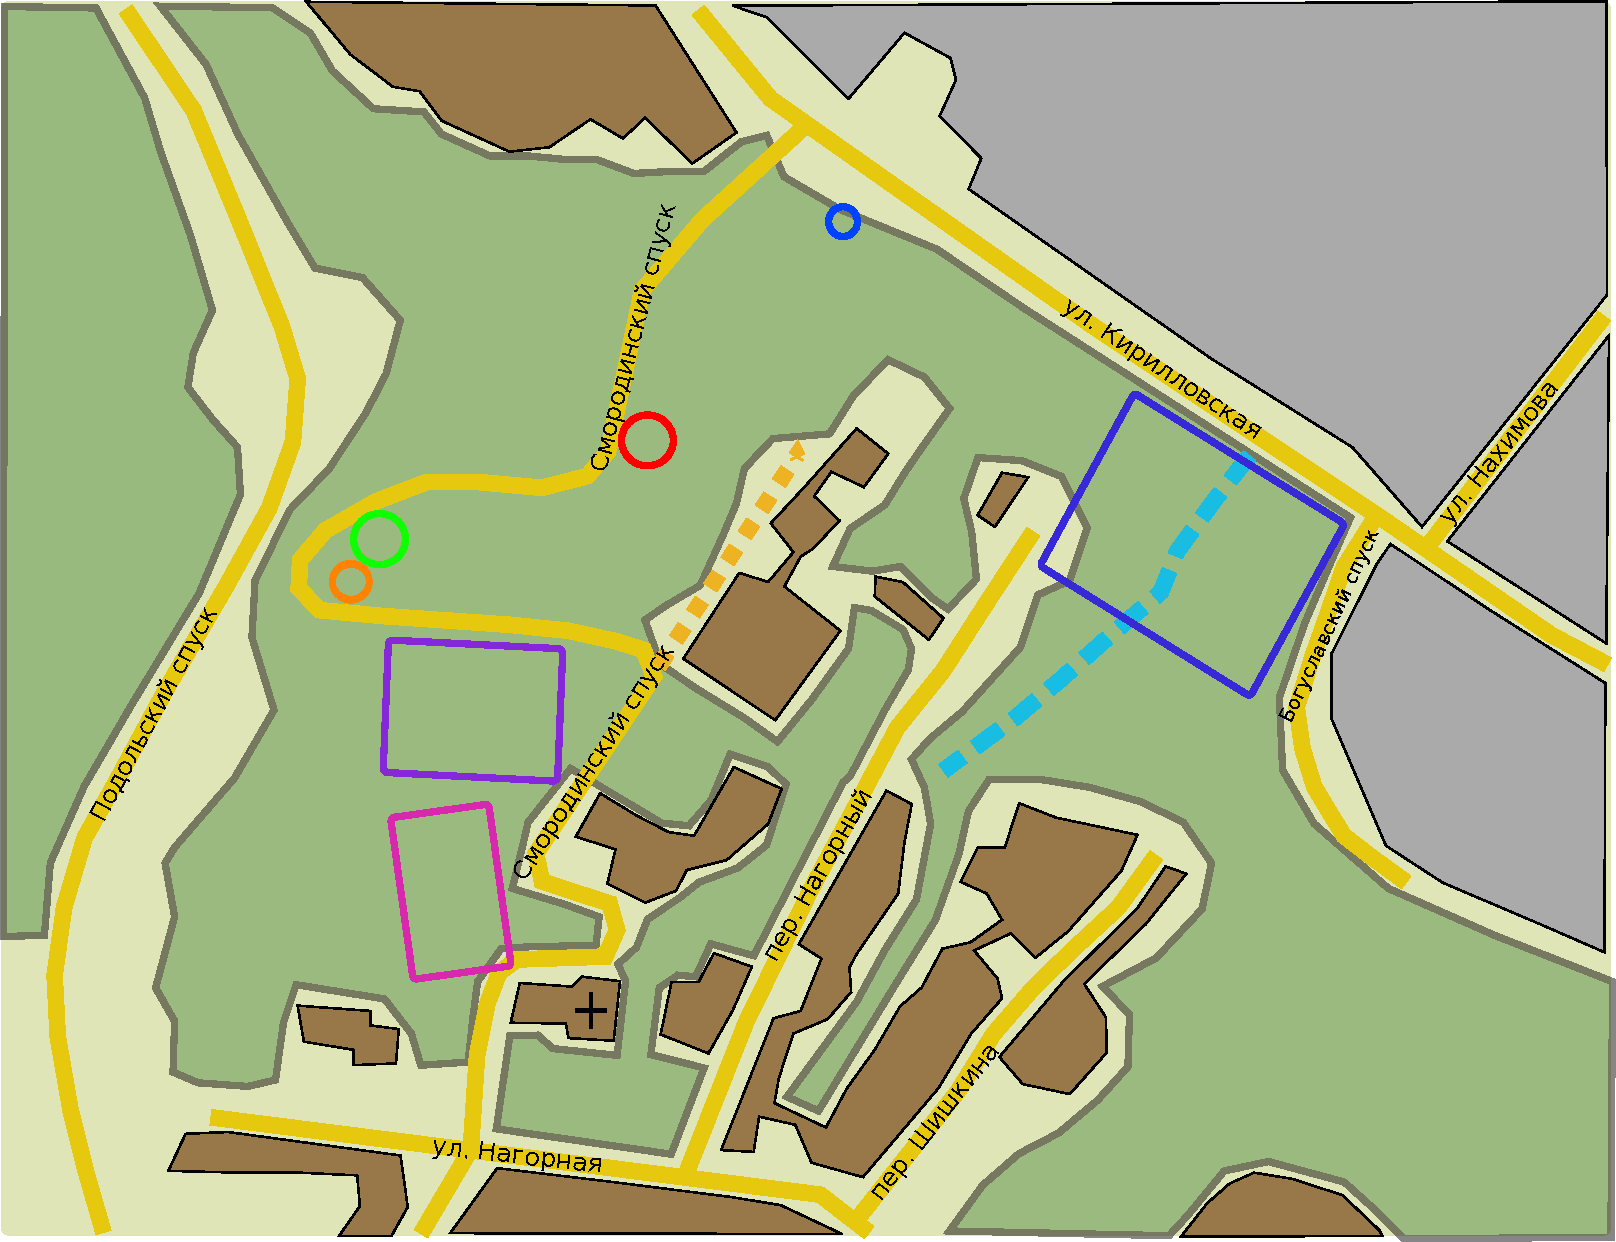
\includegraphics[width=\linewidth]{chast-zmiy/karta-opis/smor-map-2014.pdf}
\end{center}

Эта карта отражает состояние местности на 2014 год.

Легенда карты такова:

Серым цветом отмечена промзона. Промзона к северо-востоку от улицы Кирилловской лежит на низменной Оболони. В отдалении около – в разные века по-разному, но примем два километра – параллельно улице, протекала Почайна. К востоку от Богуславского спуска промзона расположена на равнине и несколько заползая на склон.

Коричневым цветом обозначена жилая застройка.

Светло-зеленым цветом отмечена местность, так или иначе заросшая лиственным лесом. Почти вся она находится на возвышенности Кирилловских высот.

Синий прямоугольник показывает примерно окрестности бывшей усадьбы Светославского. Я не знаю ее границ.

Голубая пунктирная линия – ручей в овраге близ усадьбы Светославского.

Крест – церковь Николая Чудотворца «Памяти жертв Чернобыля».

Малиновый прямоугольник – мемориал жертвам Чернобыльской катастрофы, с современным курганом.

Фиолетовый прямоугольник – бугристая местность, покрытая рощей. 

Желтоватый пунктир – грунтовка вдоль возводящихся коттеджей, она же – остаток прежней ветви Смородинского спуска.

Оранжевый кружочек – раскопанный суглинный склон, в том месте немного возвышающийся над дорогой.

Синий кружочек – совсем маленькая пещерка на обрывистом склоне.

Зеленый кружок – две пещеры в уже довольно крутом и высоком склоне над дорогой. Называю их Левой и Правой Малыми пещерами. Примерные координаты – 50°28'39.19"N 30°28'38.92"E.

Красный кружок – Кирилловская пещера, Логово Змия. Склон в том месте сильно возвышается над дорогой, пещера – ближе к его верху, вход в нескольких метрах от поверхности плато. Координаты приблизительно 50°28'41.03"N 30°28'46.32"E. 

Чтобы лучше понять настоящее, надо основательно изучить прошлое. И рассмотреть местность в связи с окрестностями, не попавшими на карту или затронутыми частично.

Итак, нарисованный «зеленый» массив более или менее отражает очертания средней части Кирилловских высот, поднимающихся над плоской Оболонью. Раньше, идя от них прочь на восток, мы бы вышли по лугам к Почайне.

Сейчас все отроги Кирилловских высот покрыты лиственным лесом. А в 1940-х, например, отрог Смородинского спуска был голым, только трава росла.

На западе крупной дорогой нисходит к Кирилловской выложенный темной брусчаткой Подольский спуск, в одном месте приблизившись к Смородинскому на 30 метров. Кирилловская и смежная с нею пещеры находятся на другом отроге, нежели Подольский спуск. Оба спуска, Подольский и Смородинский, разделены оврагом, начинающемся на уровне западной стороны того резкого колена, которое Смородинский выкидывает в месте приближения к Подольскому.

Подольского спуска раньше не было. Его проложили в середине 1950-х. При этом изменения в местности произошли следующие. 

Уничтожили верхнюю часть Смородинского спуска. Перед курганом мемориала жертв Чернобыля, на запад шла улица, отрезок Смородинского спуска – исчезла. В западной части прервали улицу Нагорную, что прежде продолжалась и соединялась с Пугачева, откуда свернувший с Овручской по Нагорной трамвайный маршрут нырял в нынешний Врубелевский спуск – улочку в Репяховом яру, что отделяет мыс Подольского спуска от горы с Кирилловской церковью.

На Куренёвку, к стадиону «Спартак» (под горой с Кирилловской церковью), спуститься можно было тремя способами. По Репяховому яру на трамвае. Узенькой Макаровской улицей, вдоль Репяхового яра гребнем холма. Смородинским спуском.

Во время прокладки Подольский спуск захватил низовья Макаровской и Репяхового яра, ручей в котором взяли в коллектор, а мостик над ручьем уничтожили. 

Главное колено Смородинского спуска начиналось южнее нынешнего –  от кургана (коего тогда не было), в целом же спуск повторял современные очертания, но с поправкой. В юго-восточном углу прежних очертаний колена, на северо-восток отделялась грунтовка. Сейчас по ее месту два отрезка. Один мощенный брусчаткой, от церкви и вниз до первого поворота. А дальше теперь вдоль особняков идет грунтовка. Справа дом\'а, слева – склон с пещерами. Грунтовка еще в пятидесятых доходила к северному склону, над улицей Кирилловской, и резко сворачивала там на запад к основной дороге Смородинского спуска. Поворот сохранился поныне, примыкая к нижней части спуска.

Прежнее колено было гораздо больше нынешнего и западной частью лежало на современном восточном склоне горы вдоль Подольского спуска. Этот спуск насквозь пробил Нагорную и Смородинский спуск, первую обрубив рукотворным оврагом, а у второго сократив петлю колена там, где теперь Смородинский и Подольский спуски сближаются. Раньше, петля Смородинского соседствовала через пустырь с Макаровской улицей.

Поглядим на аэрофотоснимок 1943 года.

\begin{center}
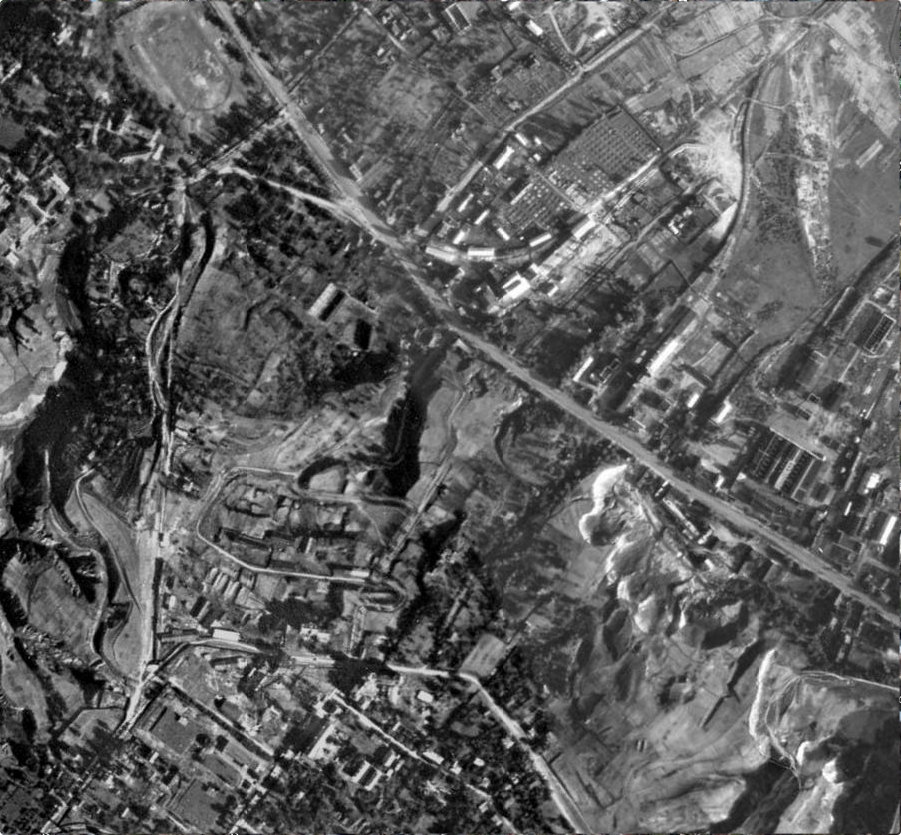
\includegraphics[width=0.80\linewidth]{chast-zmiy/karta-opis/obsh-map.jpg}
\end{center}

Главный ориентир – стадион «Спартак» в верхнем левом углу иллюстрации, и длинная прямая улица в левой части – это Макаровская. Наискосок всего кадра проходит улица Кирилловская. В нижнем правом углу виден мыс Кирилловской стоянки. Точно в середине изображения – мыс с Кирилловской пещерой, его западная граница темнеет эдаким треугольником.

На советской топографической карте тоже нет еще Подольского спуска и хорошо расписаны высоты.

\begin{center}
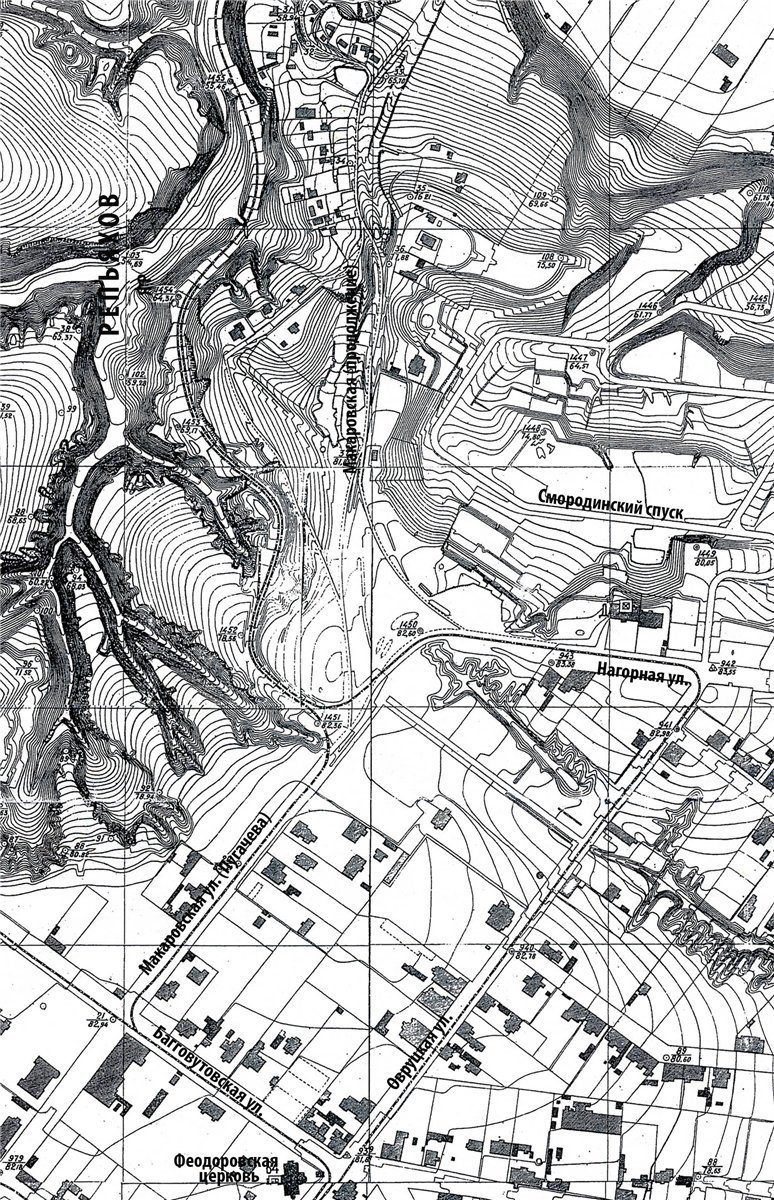
\includegraphics[width=0.80\linewidth]{chast-zmiy/karta-opis/sov-map.jpg}
\end{center}

 По всем закоулкам мы еще пройдем, в свое время, пока же сосредоточимся на Смородинском спуске.

Когда он возник как поименованный? Понятное дело, что овраг существовал и раньше, а вот название должен был получить, когда им стали пользоваться. Для спуска ли по нему, или житья в окрестностях. Рогович в 1876 году называл тамошний яр оврагом Балашова, а всю местность Загоровщиной. На 1870 год на карте обозначена «земля дочери майора Елизаветы Балаш». В то же время лежащий через водораздел Репяхов яр отмечен, под именем Кирилловского оврага, как владение Багговута.

Разберем старые карты. В первой половине 19 века на месте Смородинского спуска – дикая гора с узнаваемым яром. Чтобы добраться на Куренёвку, варианта два – по дороге от Подола вдоль Кирилловских высот (прообраз улицы Кирилловской), а если сверху от Лукьяновки – то через овраги около Иорданской церкви, либо по современной Макаровской. Тогда это была просто грунтовая дорога. Однако жилые домики уже стояли и у нижней части будущего Смородинского спуска.

В конце 19 века Смородинского спуска еще нет. Местность его и окрестностей на картах того времени подписана как «Дачи». Внизу, к северо-западу от начала будущего спуска, на месте нынешнего сквера около домов на Кирилловской 99/1К3, 99/1К2, 99/1К1, короче говоря напротив стадиона через Подольский спуск, возникла Кирилловская площадь с базаром (не путать с Куренёвской площадью и ее толкучкой, Птичьим рынком). Дом Викентия Хвойки (у него было жилье также на Игоревской 9/1) в 1911 году имел адрес Троицко-Кирилл\-овская площадь, 4 (прежнюю Троицкую площадь переименовали в Куренёвскую). Поблизости жил еще Езерский, и когда рядом под прямым углом к Кирилловской проложили новую улицу, поначалу она носила название Езерской, а потом ее переименовали в Викентия Хвойки. На площади был и разворот 18-го трамвая из Репяхового яра.

За сквером\footnote{В 1978 году при археологических раскопках примерно на этом месте, около Кирилловской, 90, нашли два культурных слоя «древнерусского времени» – как считают, 12-13 веков. Один, метровый слой, залегал на глубине 1,5 метра, затем шел песок, и на глубине 5 метров – еще полуметровый культурный слой. В первом были железные гвозди, лезвие ножа, светло-зеленые поливные плитки пола, битый кирпич, прясла, черепки. Обнаружили остатки глинобитной, толстостенной печи с полом, обложенным черепками и кусками кирпича. В печи лежали куски железного шлака или крицы, шлак валялся и рядом. Значит, тут производили из руды железо, а местность была если не частью давнего Киева, то его присёлком.} – несколько жилых домов, закрытая (в 2013 году) школа, еще некое аварийное здание – кажется, в квартале идет сплошной ремонт. Этот уголок, центром которого была Кирилловская площадь, слывет Липлиновкой, по фамилии бывшего землевладельца (психиатр Константин Михайлович Леплинский, его клиника была по адресу Кирилловская, 99). В середине 1930-х на месте площади, хат с палисадниками, огородами и пустырей создали парк с танцплощадкой и стадионом «Спартак». От большого парка теперь остался только сквер (на месте Кирилловской площади) да стадион. 

\begin{center}
\includegraphics[width=\linewidth]{chast-zmiy/karta-opis/\myimgprefix ex-kyr-plosh-2013.jpg}

\textit{2013 год, сквер на месте Кирилловской площади.}
\end{center}

На стадионе поначалу не было трибун – просто поле, пара деревянных домиков и раздевалка. Директором работал одноглазый Слуцкий, выдававший спортсменам инвентарь и форму. После войны наконец построили трибуны, тир, площадки для волейбола, тенниса, баскетбола, памятник Сталину у входа, и четыре гипсовые скульптуры атлетов. Когда именно – не знаю, на снимке 1955 года трибун еще не видно.

До 1950-х, до прорытия Подольского спуска, около стадиона был перекинут мостик через ручей, вытекавший из Репяхового яра. Леонид Коныхов в «Киевских рассказах» пишет:

\begin{quotation}
Сейчас того мостика нет. Будете искать – не найдете. Он исчез вместе с инвалидом, который продавал там самодельные конфеты в деревянном ящике со стеклянной крышкой. Мостик убрали, когда строили дорогу Подольского спуска, правую границу Липлиновки. Это еще хорошо, что Витька Шило перелетел через перила и упал с мостика в ручей, где мягкий песочек под мелкой водой.
\end{quotation}

Когда едешь с Лукьяновки выложенным трясучей, черной брусчаткой Подольским спуском, примерно на половине пути видишь справа, вровень с собой верхушки деревьев и домов – это и есть, под крутым склоном, большая часть Липлиновки. В приближении к перекрестку у стадиона, ниже, по левую руку за зеленью тоже скрывается глубина, там же – Репяхов яр, однако не зная этого, люди мельком примечают только зелень, такую же, как по горе выше, где над спуском громоздится холм со стриженым травянистым боком и рощицей наверху, граничащей с частным сектором по Макаровской.

Напротив юго-восточных зданий Липлиновки, по другую сторону улицы Кирилловской, заканчивается жилой массив и начинается промзона. К востоку от нее раньше, в виду Кирилловских высот, через поле, протекала в давнее время Почайна. Относительное расположение Почайны, цепи холмов и луговой части очень важно, о чем мы поговорим в свое время.

Карта 1911 года на месте Смородинского спуска изображает целый букет улиц! Это Димовский спуск, улица Иполитова и между ними смычка – Мишин переулок.

Снизу, к перекрестку Нагорной и Димовского спуска, присоединяется Овручская улица, как и теперь. Карты 1912-13 годов вместо букета являют пустоту. На карте 1914 года нарисована, без подписи, продолжением Овручской некая дорога с «коленом» в пределах Смородинского спуска, однако слишком прямоугольная, чтобы быть правдой.

\begin{center}
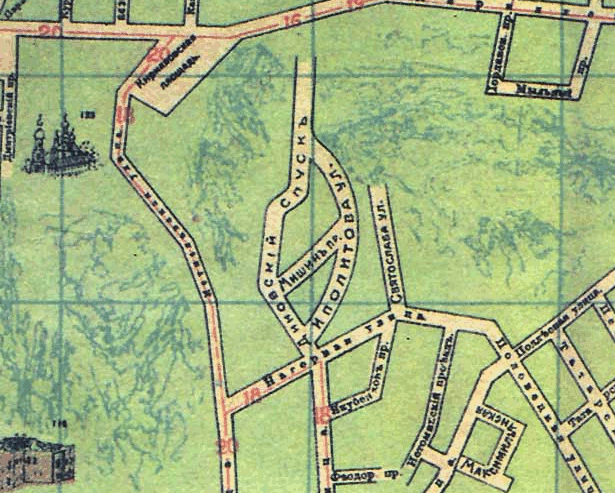
\includegraphics[width=\linewidth]{chast-zmiy/karta-opis/1911-smor-map-pal.png}

\textit{Фрагмент карты 1911 года.}
\end{center}

Затем снова картографическое забвение до 1918 года, где на немецком плане снова букет – Димовский (Диновский, Димновский?) спуск, улица Иполитова да Мишин переулок. По немецкой-то карте становятся ясными составные части будущего Смородинского спуска в виде, каким он был до прорытия Подольского спуска. Давайте поглядим вместе.

\begin{center}
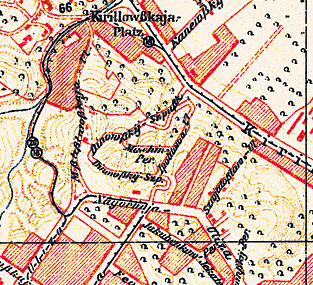
\includegraphics[width=\linewidth]{chast-zmiy/karta-opis/1918-smor-map.png}

\textit{Фрагмент карты 1918 года.}
\end{center}

Димовский спуск начинался перед местом, где ныне курган, непосредственно к югу от него. Оттуда дорога шла на запад (через разбитый в конце 2016 года сквер) в сторону Макаровской улицы. Затем видим возврат колена на восток и примерное повторение линии современного Смородинского спуска от пересечения с Мишиным переулком и ниже. 

Мишин переулок – это отрезок современного Смородинского спуска между Подольским спуском и восточным поворотом основного колена\footnote{50°28'37.5"N 30°28'46.87"E}. Наконец, улица Иполитова – то, что я именую «грунтовкой» применительно к части старого Смородинского спуска.

\begin{center}
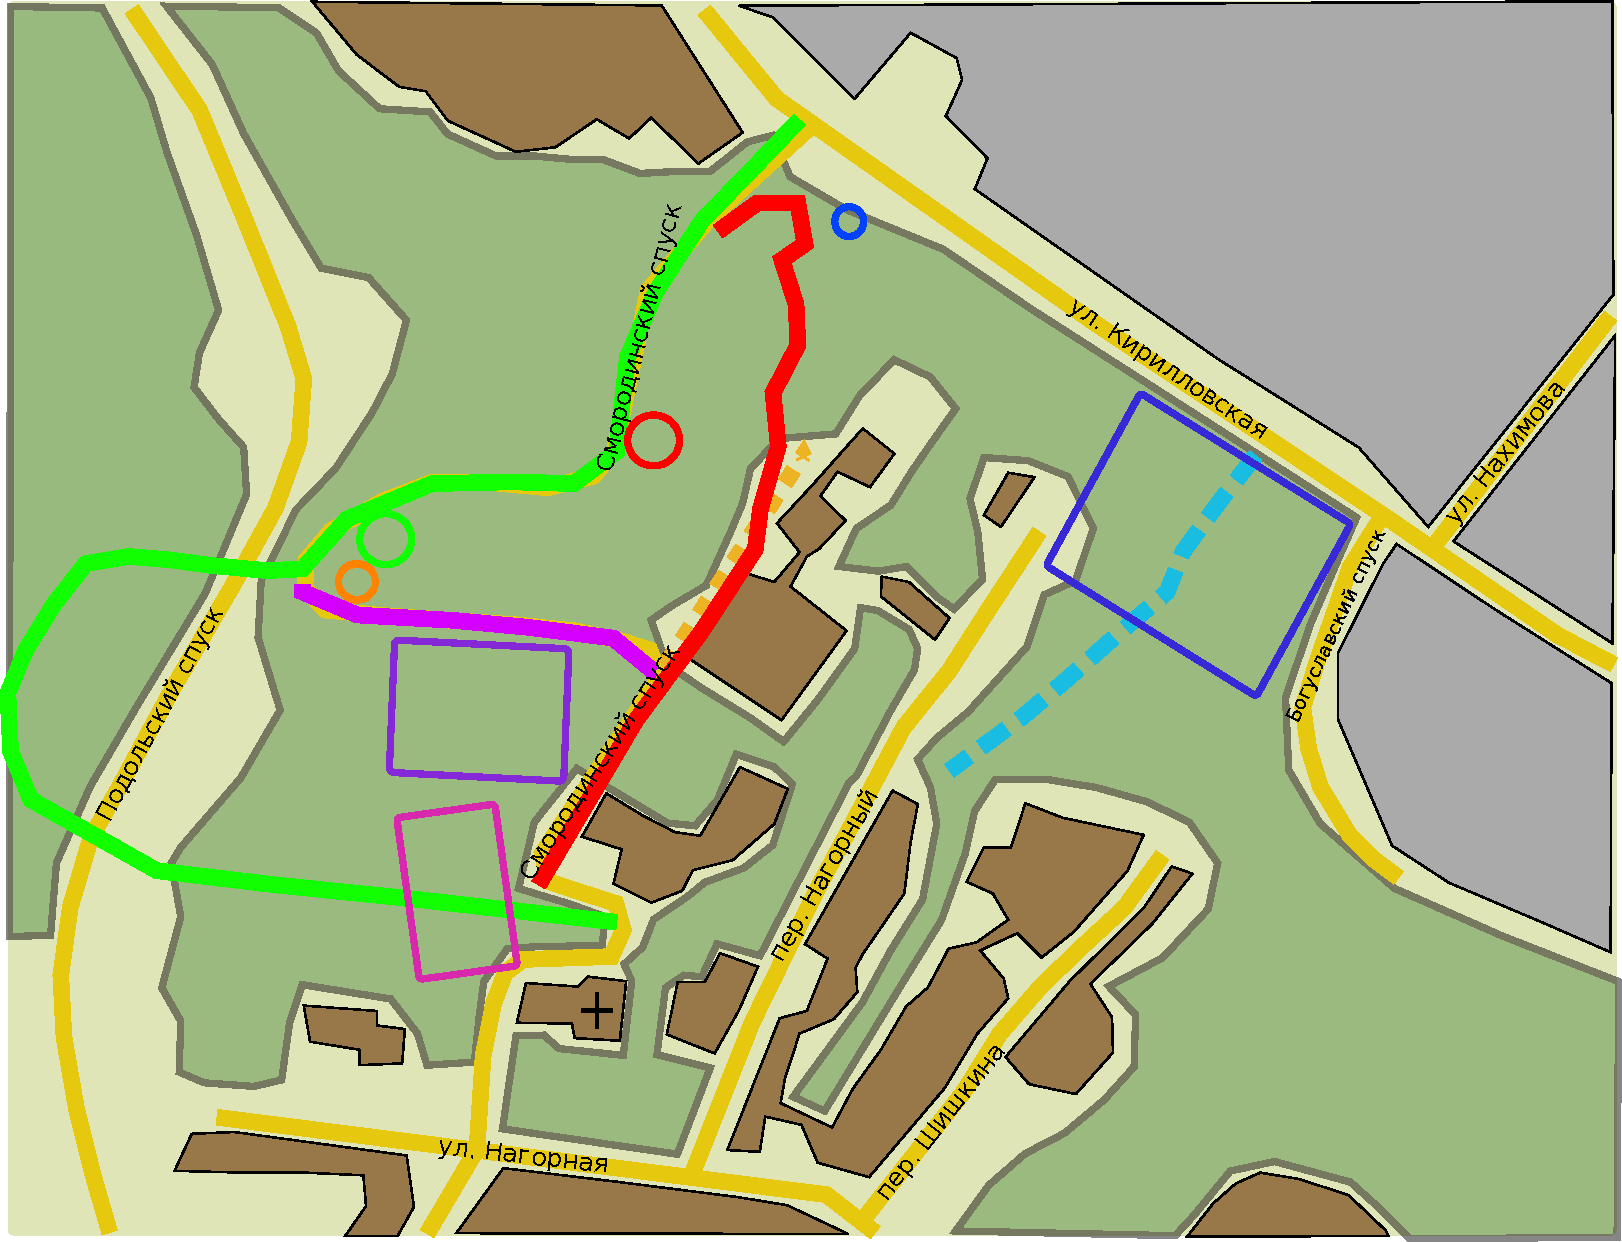
\includegraphics[width=\linewidth]{chast-zmiy/karta-opis/smor-map-1918.pdf}
\end{center}

Отмечу на основной карте линиями:

Зеленая линия – Димовский спуск.

Фиолетовая линия – Мишин переулок.

Красная линия – улица Иполитова.

На картах 1920-х годов эти улицы подписаны частично, на карте 1930-го вместо Димовского спуска явлен миру Дюковский, Мишин переулок переделывается в Мышин, а улица Иполитова теряет название, хотя обозначена. Спустя год Иполитова появляется то ли как спуск, то ли как переулок – «Іпполітівський». 

Уже в 1932 году на схеме «маршрутов и проездов» вместо этих улочек и спусков обозначен, по контуру Смородинского спуска 2014 года, но с прежним большим «коленом», «Смородиновий узвіз», выходя внизу точнехонько на Асбесто-шиферный завод. В справочниках любят писать, что спуск назвали так по старинной фамилии купцов Смородиновых. Как мы видим, переименование произошло в тридцатые годы, когда про купцов вряд ли вспомнили бы – скорее, это могла быть фамилия местного или отдаленного партийного деятеля. Также не выдерживают проверки сведения о речке Смородине.

Карта 1935 года, теперь это «Смородинський узвіз», но сохраняются переулок «Мышив» и переулок Иполитовский. На немецкой карте 1941 года есть Смородинский спуск да Иполитовский переулок. Судя по уже советской карте 1943 года, на южной части «колена», по обе стороны (то есть на отрезке, что шел мимо нынешнего кургана) было несколько зданий – два по северной стороне, три по южной. Остальная часть спуска и Мишин переулок – пусты. Здания виднеются только внизу, в районе Липлиновки вдоль улицы Кирилловской. Немцы не унимались и в 1943 году составили свою карту. Там показан Смородинский спуск – по бывшему Димовскому и по Иполитовской улице. Отмечен еще «Мышин» переулок. Такая разметка, но без Мышина, принята на отечественной карте за 1947-й. Позже от Смородинского остается только «основная» ветка, что была Димовским спуском, без отрезка от кургана до нынешнего Подольского спуска. На многих советских картах Смородинского спуска вообще нет.

Так сохранялся уголок древности, пока в 21 веке к нему не добрались вездесущие строители. Как долго продержится Смородинский спуск – неведомо. Уже трещит по швам. Поэтому важно сохранить память о нем хотя бы в книге.

Совершим прогулку, не заходя пока в пещеры. Туда мы полезем позже. Просто запечатлеем местность, как она есть в году 2014. Теперь, когда мы знаем составляющие Смородинского спуска – Димовский спуск (в варианте с урезанным коленом), Мишин переулок, Иполитовскую улицу – будет проще давать ориентиры, описывать, как к чему пройти. Вместо нелепых указаний свернуть на таком-то повороте, я просто скажу – от Мишиного переулка туда-то. 

Пещеры можно посетить, двигаясь снизу или сверху спуска. Путешествие снизу позволяет лучше погрузиться в древнее, мрачное и сказочное настроение Смородинского, зато по верху легче и быстрее! Я опишу оба пути, что позволит осмотреть верхнюю и нижнюю половины спуска.

Начнем сверху. Сюда мы доберемся от станции метро Лукьяновская пешком – полчаса ходьбы. Улицей Мельникова, затем свернем и по Герцена, вдоль парка Котляревского на улицу Овручскую. 

%Тут кстати уцелел старинный одноэтажный дом под номером 5, а в его переулке – замечательные граффити, сюжетно связанные с мультфильмом «За 80 дней вокруг света». Надпись на стене дома гласит: «Используй всё что под рукою, и не ищи себе другое».

А на другой стороне, за оградой бывшей, как в народе говорят, дачи Хрущева, в темном яру сочится из склона один из двух истоков Глубочицы – и через каскад замусоренных прудов исчезает в коллекторе. Это место – маленький тенистый парк на территории Института педиатрии, акушерства и гинекологии, мы показали в фильме «Киевская сюита». 

%\newpage

%\begin{center}
%\includegraphics[width=\linewidth]{zmiy/IMG_20130604_152101.jpg}
%\end{center}

%\begin{center}
%\includegraphics[width=\linewidth]{zmiy/IMG_20130604_151818.jpg}
%\end{center}

%\newpage

По Овручской нам идти к Нагорной, однако путь  пересекает Багговутовская. Слева, в бывшем сквере, обнесенные забором раскопки и попытки возродить церковь святого Феодора, возведенную стараниями Багговута. Здесь же был разворот трамвайного маршрута, что следовал дальше по Овручской к Нагорной, а оттуда пересекая Макаровскую в Репяхов яр и по нему до Кирилловской площади. Чуть далее от Багговутовской Овручская, застроенная там вековой давности зданиями в пару этажей, следует наверх и прямо, а Подольский спуск отделяется влево. 

\begin{center}
\includegraphics[width=0.90\linewidth]{chast-zmiy/karta-opis/\myimgprefix IMG_20130623_155220.jpg}

\textit{2013 год, вид Овручской улицы от Подольского спуска в сторону Багговутовской.}
\end{center}

По Овручской выходим на перекресток с Нагорной, даже эдакую площадь. Тишина, сонное состояние, торговый киоск родом из девяностых. Нависает здоровенная, 1940 года угловая сталинка по адресу Нагорная, 8/32 – так называемый Красный дом.

\begin{center}
\includegraphics[width=\linewidth]{chast-zmiy/karta-opis/\myimgprefix IMG_20130623_154741.jpg}

\textit{Снимок 2013 года.}
\end{center}

С другой стороны площади, над террасе над другой террасой, вплотную друг к другу стоят два старых дома, трехэтажный, 1912 года постройки, номер 5 (бывший доходный дом межевого инженера Владимира Львова, затем коммуналка Кабельного завода) и двухэтажный 7-й, построенный межевым инженером Горбуновым, а затем тоже ставший коммуналкой Кабельного. Второй этаж – деревянный. Если проведать мощеный булыжником закоулок Нагорной в сторону Подольского спуска, на самом краю горки встретим ветхий, низенький домик номер 2. Нагорная длилась и дальше, а теперь обрублена Подольским спуском. Там, где нынче рукотворный овраг, была земля, и по Нагорной к Макаровской шел трамвай в Репяхов яр.

Смородинский спуск, тоже крытый булыжником, начинает сбегать вниз от площади. Здесь он еще в хорошем состоянии. Оно ухудшается после участка стройки коллектора – асфальт сошел кусками, а булыжник сильно раздолбан, местами вывален благодаря воздействию тяжелой строительной техники. Некоторые водители рискуют машинами и пользуются этой дорогой, чтобы объехать Подольский спуск. Сокращение весьма сомнительное. На велосипеде спуск преодолеть трудно, невозможно. Сверху вниз мешает булыжник, а наоборот – крутизна.

У площади, в самом верху спуска, зеленеет скверик, выходящий к церкви Николая Чудотворца «Памяти жертв Чернобыля». По другую сторону от нее – «мемориал жертвам Чернобыльской катастрофы». Это небольшой, но узкий овраг с подвешенным колоколом. Оттуда дорожка к могучему кургану с крестом. Берега оврага, на коих любят отдыхать забредшие сюда люди, тоже напоминают курганы.

\begin{center}
\includegraphics[width=\linewidth]{chast-zmiy/karta-opis/\myimgprefix IMG_20140609_145409.jpg}
\end{center}

Что же тут было раньше? По аэрофотоснимку 1943 года здесь, на террасе с курганом – участок Смородинского спуска, видны некие огражденные участки, пять домов. Потом была ровная площадка, где росли черешни. На месте уже пустыря, между курганом и Подольским спуском, осенью 2016-го проложили дорожки сквера. А ниже к бывшему Мишину переулку, ныне виднеются земляные бугры, подозрительно похожие на остатки настоящих курганов.

%Не будем забывать, что всего в полукилометре на юго-восток отсюда Хвойка таки обозначил на своей карте курганы, примерно на той же высоте, что Мишин переулок. Да и упоминал о курганах в усадьбе Зарембских. Предположение имеет уже несколько оснований – внешний вид местности, и близость к курганам Хвойки. Да и «три могилы» с плана 1752 года припомним. Но именно «мемориальный» курган насыпан уже в наше время – это я узнал от старожила. Прежде там была полянка.

Мемориал служит началом трассы велосипедистов-да\-ун\-хильщиков. Она, через рощу за курганом срезая поворот спуска, выходит в дикую местность и проходит точно над Змиевой, Кирилловской пещерой – а поскольку там устроен трамплин, велосипедисты, не ведая, что творят, каждым веселым своим катаньем обрушивают в пещере потолок и стены.

\vspace*{\fill}

\begin{center}
\includegraphics[width=\linewidth]{chast-zmiy/karta-opis/\myimgprefix IMG_20160330_140002.jpg}

\textit{Вид от кургана в сторону Подольского спуска. Вперед – исчезнувший отрезок Димовского спуска. Справа вниз, вне кадра – Мишин переулок. Слева наверх, через несколько террас – дома 5 и 7.}
\end{center}

\vspace*{\fill}


\newpage
\begin{center}
\includegraphics[width=\linewidth]{chast-zmiy/karta-opis/\myimgprefix IMG_20160330_140047.jpg}
\textit{Вид на западный берег оврага.}
\end{center}

\begin{center}
\includegraphics[width=\linewidth]{chast-zmiy/karta-opis/\myimgprefix IMG_20160330_140050.jpg}
\textit{На восточный берег оврага.}
\end{center}
\newpage

\begin{center}
\includegraphics[width=0.97\linewidth]{chast-zmiy/karta-opis/\myimgprefix IMG_20160330_140327.jpg}

\textit{Вид с Мишина переулка наверх, на юг, к «исчезнувшему отрезку».}
\end{center}

\begin{center}
\includegraphics[width=0.97\linewidth]{chast-zmiy/karta-opis/\myimgprefix IMG_20160330_140350.jpg}

\textit{То же самое.}
\end{center}
\newpage

\begin{center}
\includegraphics[width=0.96\linewidth]{chast-zmiy/karta-opis/\myimgprefix IMG_20160330_140418.jpg}

\textit{Там же, видна терраса. На карте 1937-го, домик, некое строение было выше террасы.}
\end{center}


\begin{center}
\includegraphics[width=0.96\linewidth]{chast-zmiy/karta-opis/\myimgprefix IMG_20160330_140438.jpg}

\textit{Вид с восточного конца Мишиного переулка на северо-запад, заметен Подольский спуск.}
\end{center}

\newpage
\begin{center}
\includegraphics[width=0.99\linewidth]{chast-zmiy/karta-opis/\myimgprefix IMG_20160330_140510.jpg}

\textit{Вид с той же точки на юг.}
\end{center}

\begin{center}
\includegraphics[width=0.99\linewidth]{chast-zmiy/karta-opis/\myimgprefix IMG_20160330_140546.jpg}

\textit{Вид от колена Смородинского спуска (конец Мишиного переулка) вблизи Подольского спуска, на юг.}
\end{center}

\newpage

Вижу необходимость описывать и показывать всё подробно, ибо не знаю, что уцелеет через несколько лет. В 2016 году в окрестностях Смородинского спуска то началась очередная стройка, то сами окрестности вознамерились превратить в ландшафтный парк для народного удовольствия. Поэтому упорно держусь года 2014 (хотя предыдущая череда снимков относится к весне 2016) и продолжаю повествование.

В этих-то коричневых, поросших деревьями пустырях над Мишиным переулком мне и видятся следы давних курганов, какие-то ровные проходы в земле, не говоря уже о четко сохранившихся террасах.

Ниже церкви, Смородинский спуск, понижаясь, описывает полукруг, включающий в себя Мишин переулок. Поначалу справа возникаю особняки за кирпичными оградами, а напротив них, к западу от кургана темнеет чаща – здесь вглубь некогда уходило начало большого «колена» Димовского спуска. Но мы следуем прямо (на северо-восток), по началу прежней Иполитовской улицы, между продолжением коттеджей и рощей.

Там, где начало (восточное) Мишиного переулка, Смородинский спуск поворачивает к западу. Прямо же, на северо-восток, идет грунтовка (бывшее продолжение Иполитовской), мимо строительства новых коттеджей. Не редкость подогнанный в заповедное место подъемный кран.

Чуть левее грунтовки – чаща у обрывистого склона. Туда нам и нужно. От вытоптанной техникой глинистой площадки пучком отходит пара тропок, одна служит продолжением трассы велосипедистов, что далее раздваивается. Другая, поуже, стремится к самому краю обрыва. Нам подойдут обе, но лучше идти левой, так вы сможете осмотреть склон и не пропустить Логово Змиево. Направляемся на север. 

Долго ли, коротко. Под кромкой обрыва то и дело видны засыпанные входы. Так археологи «консервируют» то, что им больше не нужно, и не желая, чтобы туда лез кто-нибудь кроме них. От первого такого входа строго на восток, через рощу к зданиям, отходит невысокий земляной вал. 

Наконец, когда внизу сквозь деревья виднеется стройка коллектора, и Смородинский спуск делает там очередной поворот, под тропкой выглядывает небольшая утоптанная площадка. Нам туда, ко входу в Кирилловскую пещеру – но остановимся и – в пещеру, во все здешние пещеры мы полезем позже, через несколько глав.

Сейчас завершим описание местности, пройдя по Смородинскому спуску уже с его нижнего конца. От улицы Кирилловской, Смородинский отделяется на краю Липлиновки, чуть южнее улицы Хвойки. Неприметный поворот за высоким зданием под номером 85, и – мы поднимаемся по дороге с вывороченным булыжником и слезшим асфальтом.

Слева, на востоке, сразу высится и тянется дальше гора, именно там надо высматривать пещеры. Обзор зависит от времени года. Летом в зелени черт поймешь, но вот осенью или ранней весной – хорошо. А сторона, обращенная к Липлиновке и Подольскому спуску, более пологая, хотя в местами поднимается вровень с левым берегом.

\begin{center}
\includegraphics[width=\linewidth]{chast-zmiy/karta-opis/\myimgprefix IMG_2688.jpg}
\end{center}

Через решетки у обочины слышно журчание воды – она бежит постоянно, значит, даже если это ливнесток, то в него выведены грунтовые воды.

Стройкой коллектора занято удолье между берегами оврага, поэтому правый его берег толком исследовать не могу. А вот на другом, слева от дороги, и находится Змиева, Кирилловская пещера. 

\begin{center}
\includegraphics[width=\linewidth]{chast-zmiy/karta-opis/\myimgprefix IMG_2689.JPG}
\end{center}

Снизу ее не заметишь, если не знаешь, что этот обвал на склоне продолжается до самой площадки у входа в пещеру.

До строительства сверху на горе и внизу под нею не было особых размывов склона, оползней и прочего. Суглиновые, местами замшелые залысины на склоне просматривались ближе к плато, сам же склон покрывала сухая листва. Сейчас ее меньше, а следов сползания грунта и обвалов всё больше.

От стройки Смородинский спуск сворачивает в сторону Подольского, в каком-то месте они едва не сходятся, разделенные узким перешейком и подпорной стенкой. Немного не доходя, слева мы видим входы в две, как я их называю, Малые пещеры:

\begin{center}
\includegraphics[width=\linewidth]{chast-zmiy/karta-opis/\myimgprefix malaya-peshera-01.jpg}
\end{center}

И туда мы полезем позже.

От точки, где оба спуска почти соединяются, на восток идет отрезок пути, бывший Мишиным переулком. По правую руку – пологий склон в буграх. Ну а если пойти налево, выберемся ко краю плато, и тропка вдоль обрыва выведет всё к той же Кирилловской пещере.

В дореволюционной книжке на польском языке «Kijow i jego pamiatky» я нашел любопытную иллюстрацию: 

\begin{center}
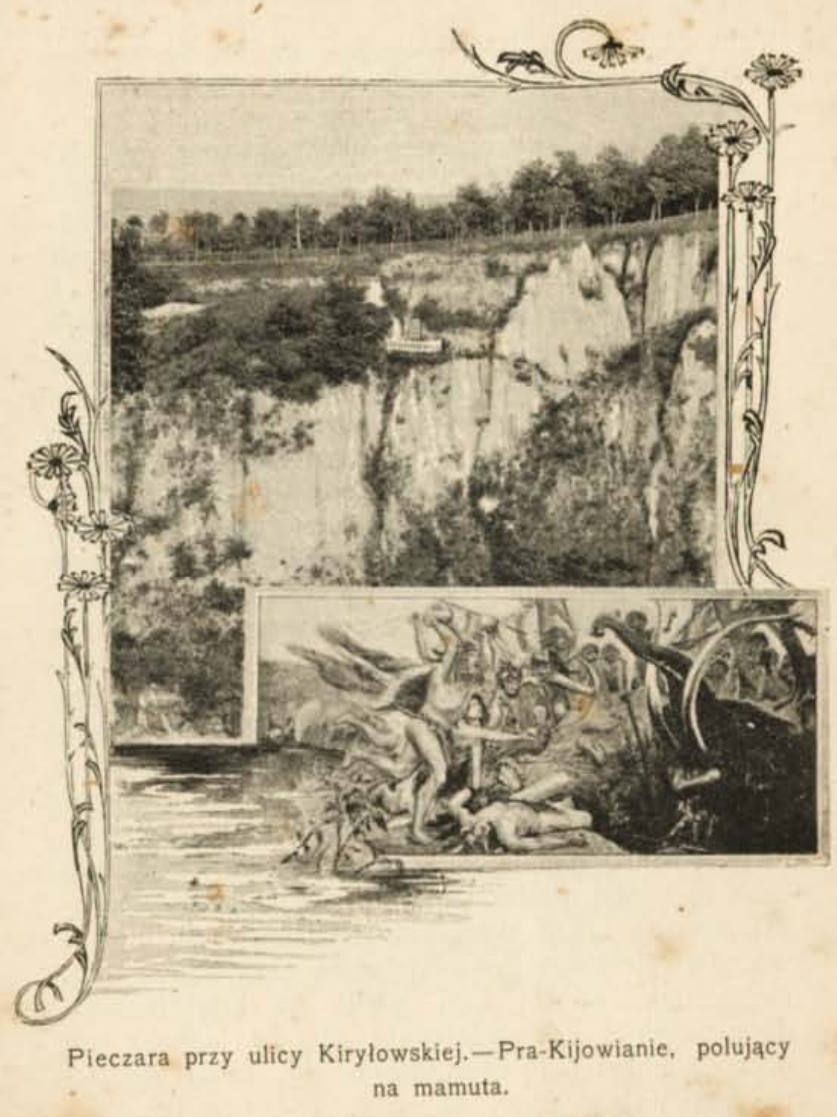
\includegraphics[width=\linewidth]{chast-zmiy/karta-opis/polska.jpg}
\end{center}

Подпись в переводе гласит: «Пещера возле улицы Кирилловской. Пра-киевляне, охота на мамонта».

Выдумку художника оставим в стороне, мне любопытна фотография. В тексте книги ей предшествует рассказ о раскопках Хвойкой Кирилловской стоянки, а также поверхностно повествуется об исследованиях здесь же Антоновича, поэтому неясно, к чему относится снимок – то ли в самом деле это старейший известный снимок окрестностей Смородинского спуска и где-то там можно усмотреть вход в Змиеву пещеру, то ли это склон у глинища Зайцева, возле Кирилловской стоянки. По фотографии трудно судить о высоте и невозможно определить изображенное место.

Итак, мы прошлись по Смородинскому спуску сверху вниз, потом снизу вверх, но в последнем случае больше держались дороги. Остается уделить внимание плато, лежащему на восток от последнего отрезку Смородинского спуска – между ним, бывшей улицей Ипполитовской, да Кирилловской. Поверхность того самого отрога, где в западном склоне находится вход в Змиеву пещеру.

Этот обрывистый склон имеет почти ровное направление с юга на север. Между коттеджами вдоль «грунтовки» и Смородинским спуском, или, если угодно – от коттеджей до обрыва – осталась роща шириной 60-100 метров, покрывающая наклонное в сторону Кирилловской улицы плато.  Роща изуродована мусором и двумя велотрассами, где оборудованы трамплины и разные витиеватые заезды.

Смежная, северная сторона отрога, хотя и лежит много ниже верховьев Смородинского спуска, всё равно внушительной кручей нависает над Кирилловской улицей. Попав туда, замечаешь, что местность неестественно изрыта – это, полагаю, следы деятельности Багговутов.

«Грунтовка», теряющаяся ныне в роще, имеет продолжение, съезд в виде изгиба давней дороги – он прорезает отрог, и одновременно огибает его с севера, выходя к Смородинскому спуску. На дне изгиба в точке, где он уже взобрался на плато – остатки мостовой из мелкого темного камня.

Не знаю, сколь справедлива догадка, но это место, по сам\'ой закругленности дороги, зажатой в ущелье, кажется мне раскопанной спиралевидной (как Змиева) пещерой, каких по словам профессора Роговича тут было несколько. Багговуты могли разрыть ее, а затем на основе раскопа возникла дорога.

Поглядим на картинки за август 2016 года. 

%Я  временно изменю своему правилу описывать местность 2013 года.

\begin{center}
\includegraphics[width=0.89\linewidth]{chast-zmiy/karta-opis/\myimgprefix IMG_20160813_152546.jpg}

\textit{Роща на плато, тропка вдоль кромки обрыва.}
\end{center}

\begin{center}
\includegraphics[width=0.89\linewidth]{chast-zmiy/karta-opis/\myimgprefix IMG_20160813_152652.jpg}

\textit{Трамплин над Змиевой пещерой.}
\end{center}

\newpage

\begin{center}
\includegraphics[width=0.73\linewidth]{chast-zmiy/karta-opis/\myimgprefix IMG_20160813_153030.jpg}

\textit{Вид от того или другого трамплина на север.}
\end{center}

\begin{center}
\includegraphics[width=0.73\linewidth]{chast-zmiy/karta-opis/\myimgprefix IMG_20160813_153330.jpg}

\textit{Раскопанный северный склон.}
\end{center}

\newpage

\begin{center}
\includegraphics[width=0.73\linewidth]{chast-zmiy/karta-opis/\myimgprefix IMG_20160813_153931.jpg}

\textit{Нижняя часть дороги в «загогулине».}
\end{center}

\begin{center}
\includegraphics[width=0.73\linewidth]{chast-zmiy/karta-opis/\myimgprefix IMG_20160813_153748.jpg}

\textit{Часть несколько выше.}
\end{center}

\newpage

Когда идешь от Змиевой пещеры дальше вдоль кромки склона на север, приближаясь к «загогулине» и чудовищно изрытой северной стороне горы, замечаешь несколько вещей. 

Кромка обрыва очень ровная. То и дело около нее какие-то раскопы – ямы. Одна из них довольно большая, глубиной по шею, и превращена в свалку. Летом 2013 года она была примечательна странностью, позже исчезнувшей. В третью редакцию книги эти сведения не вошли – я не желал нарушить покой крыс. Ныне они сгинули, я волен рассказать. 

Ну ничего удивительного в мусоре, вероятно стащенном сюда строителями. Кострище с обугленными бутылками, ведра от краски, испорченные стройматериалы, прочий мелкий хлам, недостойный описания, разве что – съестного нет. Это важно, ибо яма кишела крысами. Значит, их привлекало туда нечто иное, не еда.

В стенах ямы были прокопаны галереи, укрепленные досками и колышками. Местами коридоры были открытыми, как бы подземный ход в разрезе. Кое-где в суглинок просто уходили норы. Крысы бегали в этих галереях, показывались из нор, исчезали в них.

Со дна ямы торчало сооружение, сложно поддающееся описанию. Упрощенно – сухой ствол дерева да шест, между ними перекладина. Шест  вставлен в полый остаток какого-то другого дерева, причем туда же помещены вертикально пять или шесть коротких палок. На верху шеста, из колышков, сделано подобие уключины, куда вставлен один конец перекладины, другой же покоится на второй уключине (уже без верхней палочки) – на дереве.

Вокруг с тихим шорохом сновали крысы, и казалось, что всё это какой-то крысиный городок, чья-то непонятная забава. Нечто, имеющее назначение, которое не вычисляется случайным прохожим, ибо подобия этому в обыденности не существует, а осмыслить эти галереи и деревянное сооружение логическими рассуждениями не получается. 

Допустим, крысы могли сделать норы, однако не укрепленные коридоры и сооружение из дерева. В чем же дело? Сумасшедший строитель мастерил тут после смены? Или велосипедисты проводили свой досуг? Они устраивают на велотрассах разные мостики, трамплины, однако то распознаётся однозначно.

Из подобного мне память подсовывает только странные горбы с норами около Кирилловской стоянки, хотя я не видел там ни галерей, ни крыс, ни деревянных сооружений.

Далее снимки 2013 года. 

\begin{center}
\includegraphics[width=0.90\linewidth]{chast-zmiy/karta-opis/\myimgprefix IMG_20130728_145852.jpg}

\textit{Яма и сооружение, вид в сторону обрыва.}
\end{center}


\newpage
\vspace*{\fill}
\begin{center}
\includegraphics[width=\linewidth]{chast-zmiy/karta-opis/\myimgprefix IMG_20130728_145959.jpg}

\textit{Яма и сооружение, вид в сторону обрыва, на запад.}
\end{center}
\vspace*{\fill}


\newpage

\vspace*{\fill}
\begin{center}
\includegraphics[width=\linewidth]{chast-zmiy/karta-opis/\myimgprefix IMG_20130728_150110.jpg}

\textit{Сооружение, вид на восток.}
\end{center}
\vspace*{\fill}

\newpage

\begin{center}
\includegraphics[width=\linewidth]{chast-zmiy/karta-opis/\myimgprefix IMG_20130728_145949.jpg}

\textit{Общий вид ямы.}
\end{center}

\begin{center}
\includegraphics[width=\linewidth]{chast-zmiy/karta-opis/\myimgprefix IMG_20130728_145940.jpg}

\textit{Общий вид ямы.}
\end{center}

\newpage

\begin{center}
\includegraphics[width=\linewidth]{chast-zmiy/karta-opis/\myimgprefix IMG_20130728_150023.jpg}

\textit{Общий вид ямы.}
\end{center}

\begin{center}
\includegraphics[width=\linewidth]{chast-zmiy/karta-opis/\myimgprefix IMG_20130728_150052.jpg}

\textit{Укрепленный «бортик» ямы.}
\end{center}

\newpage
\vspace*{\fill}

\begin{center}
\includegraphics[width=\linewidth]{chast-zmiy/karta-opis/\myimgprefix IMG_20130728_150117.jpg}

\textit{Участок галерей.}
\end{center}
\vspace*{\fill}
\newpage

\vspace*{\fill}
\begin{center}
\includegraphics[width=\linewidth]{chast-zmiy/karta-opis/\myimgprefix IMG_20130728_150123.jpg}

\textit{Сооружение. Ствол, куда вставлен и закреплен шест с «уключиной» наверху. Обратите внимание на вертикальные палки в нижней пустоте ствола.}
\end{center}
\vspace*{\fill}
\newpage

В 2020 году яма есть, свалка есть, да от прочего не осталось почти и следа.

Мне не терпится приступить к самому интересному – Змиевой пещере – я намеренно откладываю это, чтобы материал получился наиболее полным. И мало мы еще рассмотрели окрестности Смородинского спуска – надобно посетить еще смежную с ним местность, а это гора с Кирилловской церковью и яры по обе ее стороны – Репяхов да Бабий.

\chapter{Святой Кюрила}

Как его только не называли в летописях, монастырь сей. И святой Кюрила, Курило, и Кирилловский – суть не меняется. Познакомимся с монастырем и церковью, давшими имя высотам, а заодно со зловещими ярами по обеим сторонам горы, на которой стоит эта церковь.

От Смородинского спуска недалече. Я придерживаюсь положения, что упомянутые в сказаниях несколько пещер, где обитал Змей – это пещеры именно на Смородинском спуске. И что тамошняя спиралевидная пещера, описанная Антоновичем, она же главная героиня фильма «Логово Змия» – и есть упоминаемая в источниках Кирилловская или Змиева пещера.

Однако не всё так четко и ясно.

На привязку Змея к Смородинским пещерам указывает неясная штука – людская молва, изустное предание. Некие люди живут, помнят что-то, передают словами другим людям, а те далее, с течением времени. Так в народе сохраняется память. Быть может, несколько веков назад ребенок спросил у деда – а что это за пещера? Тот вспомнил – здесь жил Змей. Ребенок вырос, состарился, сам стал дедом, и уже в ответ своему внуку поведал ту же историю. Но если внук задал вопрос о другой пещере, близлежащей, а дед решил, что речь идет об известной ему, деду, пещере? Так молва способна перенести название с одной пещеры на другую, исказить предание.

И не грех обозреть окрестности, чтобы выяснить, какие еще тут существуют пещеры и подходят ли они под название Кирилловской. Именно Кирилловской, остальное нас не касается, потому что Кирилловская пещера однозначно связана с легендами со Змеем. Кирилловская пещера точно является Змиевой пещерой. Но является ли спиралевидная пещера на Смородинском спуске – Кирилловской пещерой? На этот вопрос нельзя ответить положительно с полной уверенностью, хотя по совокупности доводов можно так считать.

Рассмотрим вначале упрощенную карту, которая поможет в дальнейшем рассказе.

\begin{center}
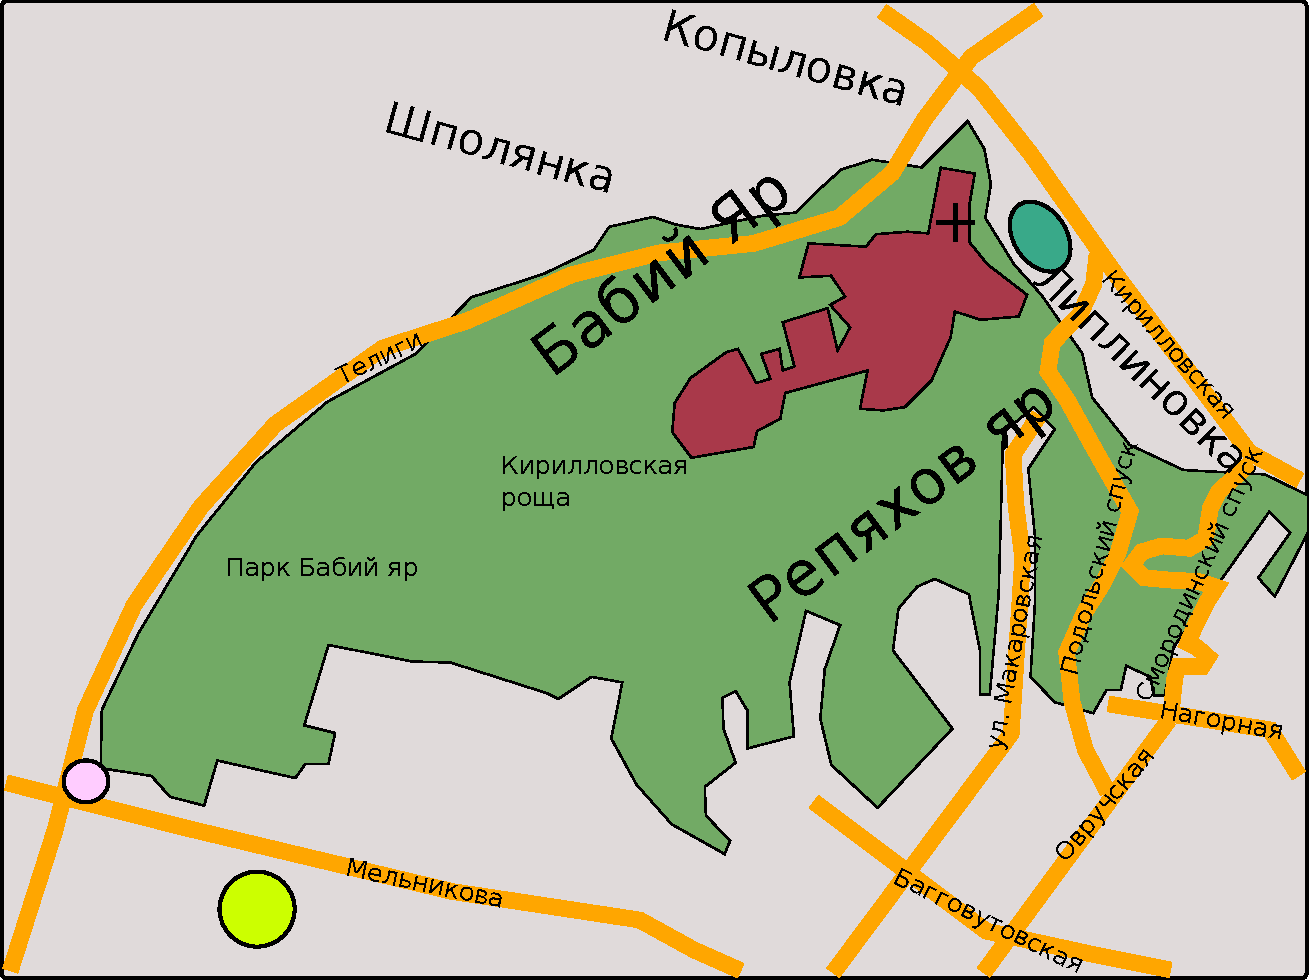
\includegraphics[width=\linewidth]{chast-zmiy/kurilo/kyr-okr.pdf}
\end{center}

Многие улицы я выпустил, лень было рисовать. Мне важно просто отметить взаимное расположение урочищ.

Крестом обозначена Кирилловская церковь. 

Зеленая область – парки, рощи, просто заросли.

Вишневого цвета область – территория психбольницы имени Павлова, бывший Кирилловский монастырь.

Улица Макаровская вообще-то делится на Пугачева и Макаровскую. Раньше границы Макаровской ездили туда-сюда, а северный отрезок нынешней Макаровской назывался улицей Мстиславской, которая иногда заменяла всю Макаровскую. Всё это неважно для предмета нашего разговора.

Салатовый кружок – телебашня.

Розовый кружок – станция метро «Дорогожичи».

Овал цвета морской волны – стадион «Спартак».

Теперь начнем повсюду бродить.

Под горой с церковью сейчас находится стадион «Спа\-ртак». У него старая еще, середины прошлого века, кованая, будто из скрепленных копий, ограда с буквами «С».

\begin{center}
\includegraphics[width=\linewidth]{chast-zmiy/kurilo/\myimgprefix IMG_2674.JPG}

\textit{Снимок 2013 года.}
\end{center}

13 марта 1961 года она была залита по самые наконечники пульпой. Годами, Петровские кирпичные заводы на Сырце\footnote{Сохранившийся от них карьер, ставший озером, находится по координатам 50°29'10.85"N 30°26'48.17"E. Это в двухста с лишком метров к югу от восьмидесятых номеров по улице Сырецкой.} гнали по трубам непригодную к производству породу, смешанную с водой, в Бабий яр, находящийся к северу за горой. Дамбу яра прорвало и отходы хлынули вниз. Грязь обрушилась на Куренёвку и погребла под собой сотни, если не тысячи людей. Об этом написано несколько книг и множество статей, это отдельный разговор, как и сам Бабий яр.

Гору с Кирилловской церковью издревле сторожили два длинных и глубоких яра – Бабий с севера и Репяхов с юга. Бабий яр известен в истории по учиненным гитлеровцами расстрелам в 1941 году и по Куренёвской трагедии 61-го. Пожалуй, трудно сыскать в мире место с более мрачной историей.

Сейчас некоторые пишут – мол, никаких расстрелов в Бабьем яру не было. Может и войны не было?

Осенью 1941 года в яру начались расстрелы – и первыми были убиты 752 пациента Павловки, психиатрической больницы на территории бывшего Кирилловского монастыря. Спустя два дня, 27 сентября, немцы «пригласили» в Бабий Яр евреев.

С ним связана беда и моих предков по материнской линии, хотя и не евреев.

Прадед и прабабушка, Федор Максимович и Марфа Семеновна Бородины в 1930-х перебрались в Киев из села Непхаево, что в Белгородской области. 

Сорваться с родных мест, где дети боярские (было такое сословие, оно же однодворцы) Бородины и Черняевы жили по крайней мере с 17 века, вынудили обстоятельства. Федор Максимович был среди братьев старшим, служил в колхозе конюхом. А брат его Охрим работал начальником железнодорожной станции в Самаре. И прислал большаку письмо – мол, растратил казенные деньги, что делать?

Федор Максимович продал дом, корову Зорьку, лошадь, и поехал со всей семьей – женой и дочкой Таней (моей бабушкой) в Самару. Там, отдав Охриму большую часть денег, Бородины купили себе домик «в центре города», однако не смогли там жить, потому что местные говорили на непонятном языке, были чужими.

Бородины вернулись в Непхаево, где над ними смеялись – дескать, ездили в погоне за длинным рублем! Бородины ведь скрыли охримову растрату. 
 
Федор Максимович подался на заработки (он был еще и столяром) в Харьков, а накопив денег и получив какой-то посул работы в Киеве, отправился с семьей сюда, где поселился в коммунальной квартире в подвальном помещении флигеля усадьбы Беляшевских, на Чкалова 43\footnote{В адресных книгах 1882 года по адресу Мало-Владимирская, 41 живет «священник Беляшевский», в 1899 году дом имеет номер 43, а живет там Стемпниовский А. М., и по крайней мере в 1906-1914 годах – «Стемпниовская Ольга Як.».}, квартира 28. Сейчас этот дом носит адрес Гончара, 43-В.

Федор Максимович устроился работать продавцом в продуктовом магазине «на Золотоворотской улице», а потом столяром в «военную часть» неподалеку. Марфа же работала уборщицей у военных в доме около Золотых ворот, а потом уборщицей в НКВД и рассказывала, как нквдшники рассовывали себе по карманам лежащие на столах конфискованные украшения, а она подбирала упавшие и клала обратно на стол.

От военной части Бородины получили комнату в коммунальной квартире в семиэтажке напротив пожарного депо на Короленко (Владимирской), 13. Позже, после взрыва здания немцами, переселились на второй этаж самого депо.

Тут я несколько путаюсь, потому что бабушка говорила и про частичный взрыв дома на Чкалова, и что потом его восстанавливали после войны. И в какой военной части работал прадед, тоже непонятно – возможно на улице Ярославов вал.

На пригорке над домом на Чкалова\footnote{Улица перпендикулярна к Ярославову валу, спускается от него вниз.} в самом деле была «военная часть», и от нее сохранился довоенный еще бункер, ниже дома Сикорских (Ярославов вал, 15-Б). Вообще этот бункер во время войны относился к штабу и командному пункту Киевского корпуса ПВО (7-й корпус ПВО). До войны, командный пункт в бункере (Ярославов вал, 15-А) был в распоряжении 3-й дивизии ПВО, по крайней мере с 1938 года.

Над бункером, выше по горе – уцелевший дом Сикорских. Он стоит во дворе выходящего на Ярославов вал пятиэтажного серого здания под номером 15, известного как бывшая военная гостиница «Красная звезда». Она построена на месте одноэтажного другого дома Сикорских. В обоих и старых зданиях, и позже в нововыстроенном размещался штаб ПВО. Командный пункт около бункера был в ведении ПВО до 1968 года.

На горке между трехэтажным домом Сикорских и флигелем Беляшевских еще в советское время построили также белопанельный дом для высшего командного состава, но там жили и партийцы да ученые, в том числе академик Глушков. Бункер же в 70-е переоборудовали под убежище гражданской обороны.

По словам бабушки Тани, немцы при отступлении «за Днепр» выгоняли всех из близлежащих домов, и дом где Бородины жили частично взорвали. О каком доме идет речь – на Чкалова или Короленко – я не понимаю. Изгнанная из дому, прабабушка Марфа с маленьким сыном Сашей перебралась в деревню Кожанку Киевской области, под Фастовом. 

Этому предшествовала гибель Федора, после которой Марфа и Саша пряталась сначала в лесах под Киевом, комнату же занял дворник. Здесь я свожу воедино данные из рассказов бабушки разных лет, поэтому очень сложно. Бабушку в описываемое время, еще до смерти ее отца, угнали в Германию. А прабабушка после освобождения Киева, вернулась в город и жила где-то на Большой Житомирской.

Где бы ни жили Бородины во время войны – на Короленко ли, на Чкалова ли, у них были соседи – еврейская семья, супруги, с дочкой примерно пяти лет, по имени Майя. Отец Майи еще до войны был военным и с нападением фашистов ушел на фронт, а жена его с дочерью остались в Киеве.

Мать Майи отправилась в Бабий яр, а Майю Бородины спрятали сначала у себя, а потом Федор Максимович куда-то ее переправил в безопасное место, к родственникам девочки или к знакомым, непонятно.

После этого другие соседи «заложили» Бородиных (за такую услугу немцы платили), в подвал пришли полицаи и отвели Федора Максимовича в гестапо, где фрицы его избили, и как бабушке потом рассказывали – ее отец умер от побоев уже в Октябрьской, ныне Александровской больнице и похоронен там в братской могиле, которую я не могу найти.

В конце семидесятых, при строительстве на территории больницы, во время земляных работ находили черепа.

Несколько раньше Бородиным удалось спасти военного врача, Николая Филипповича (Пилиповича) Шило из села Александровки Бобровицкого района, Черниговской области. При отступлении советских войск судьба забросила его в Киев к двоюродному брату, того не оказалось дома, но приютили Бородины, лечили и кормили, пока в городе не стало совсем опасно. 

Николай начал пешком пробиваться домой, вместе с моей бабушкой Таней, которую родители хотели отправить подальше от города. Три дня пешком до станции Кобыжчи. Позже, как только бабушка вернулась в Киев – потянуло проведать – её угнали на работы в Германию. И Шило, узнав об этом, рвал на себе волосы и говорил: «Зачем я ее отпустил в Киев?».

А попасть в Германию было очень просто – идешь себе к Сенному рынку, вдруг облава, оцепление, тащат в немецкую комендатуру на Артёма, 24. И наутро, как есть, без вещей, везут на вокзал и грузят в полувагоны для скота, без крыши и дверей. Пересадка в Дрездене. Потом – «биржа труда», являются местные бюргеры на велосипедах, выбирают себе в рабы славян.

В Бабьем яру расстреливали не только евреев – жертвами пали военнопленные, цыгане, коммунисты, подпольщики. В 1943 году, когда наши освободили Киев, побывал там и корреспондент «Правды» Борис Полевой. Потом он вспоминал:

\begin{quotation}
Мы вошли в Киев с первыми советскими частями.  Город еще пылал. Но всем нам корреспондентам, не терпелось побывать в Бабьем Яру. О нем мы слыхали в эти годы предостаточно, но нужно было увидеть все самим. Сейчас уже не помню фамилию той женщины, которая взялась нас туда проводить. Помню только, кажется, что она была учительницей и пережила оккупацию. Мы приехали на Бабий Яр и обмерли. Громадные глубоченные рвы. Накануне бомбили город, и одна из бомб попала в откос яра. Взрывом откололо внизу кусок склона. И мы увидели непостижимое: как геологическое залегание смерти – между слоями земли спрессованный монолит человеческих останков. Даже в самом страшном сне такое не привидится... Не верилось, что все это может быть. Страшно... Очень страшно даже вспоминать об этом... Более страшного я не видел за всю войну. Потом были Освенцим, Дахау, Бухенвальд, десятки других мест массового уничтожения людей. Но самое страшное, уму непостижимое было там, в Бабьем Яру.
\end{quotation}

На снимках Johannes Hahle, фотографа 637-го немецкого отряда пропаганды 6-й армии Вермахта –  Бабий яр в 1941 году. Пленные советские граждане закапывают тела и вещи убитых.

\begin{center}
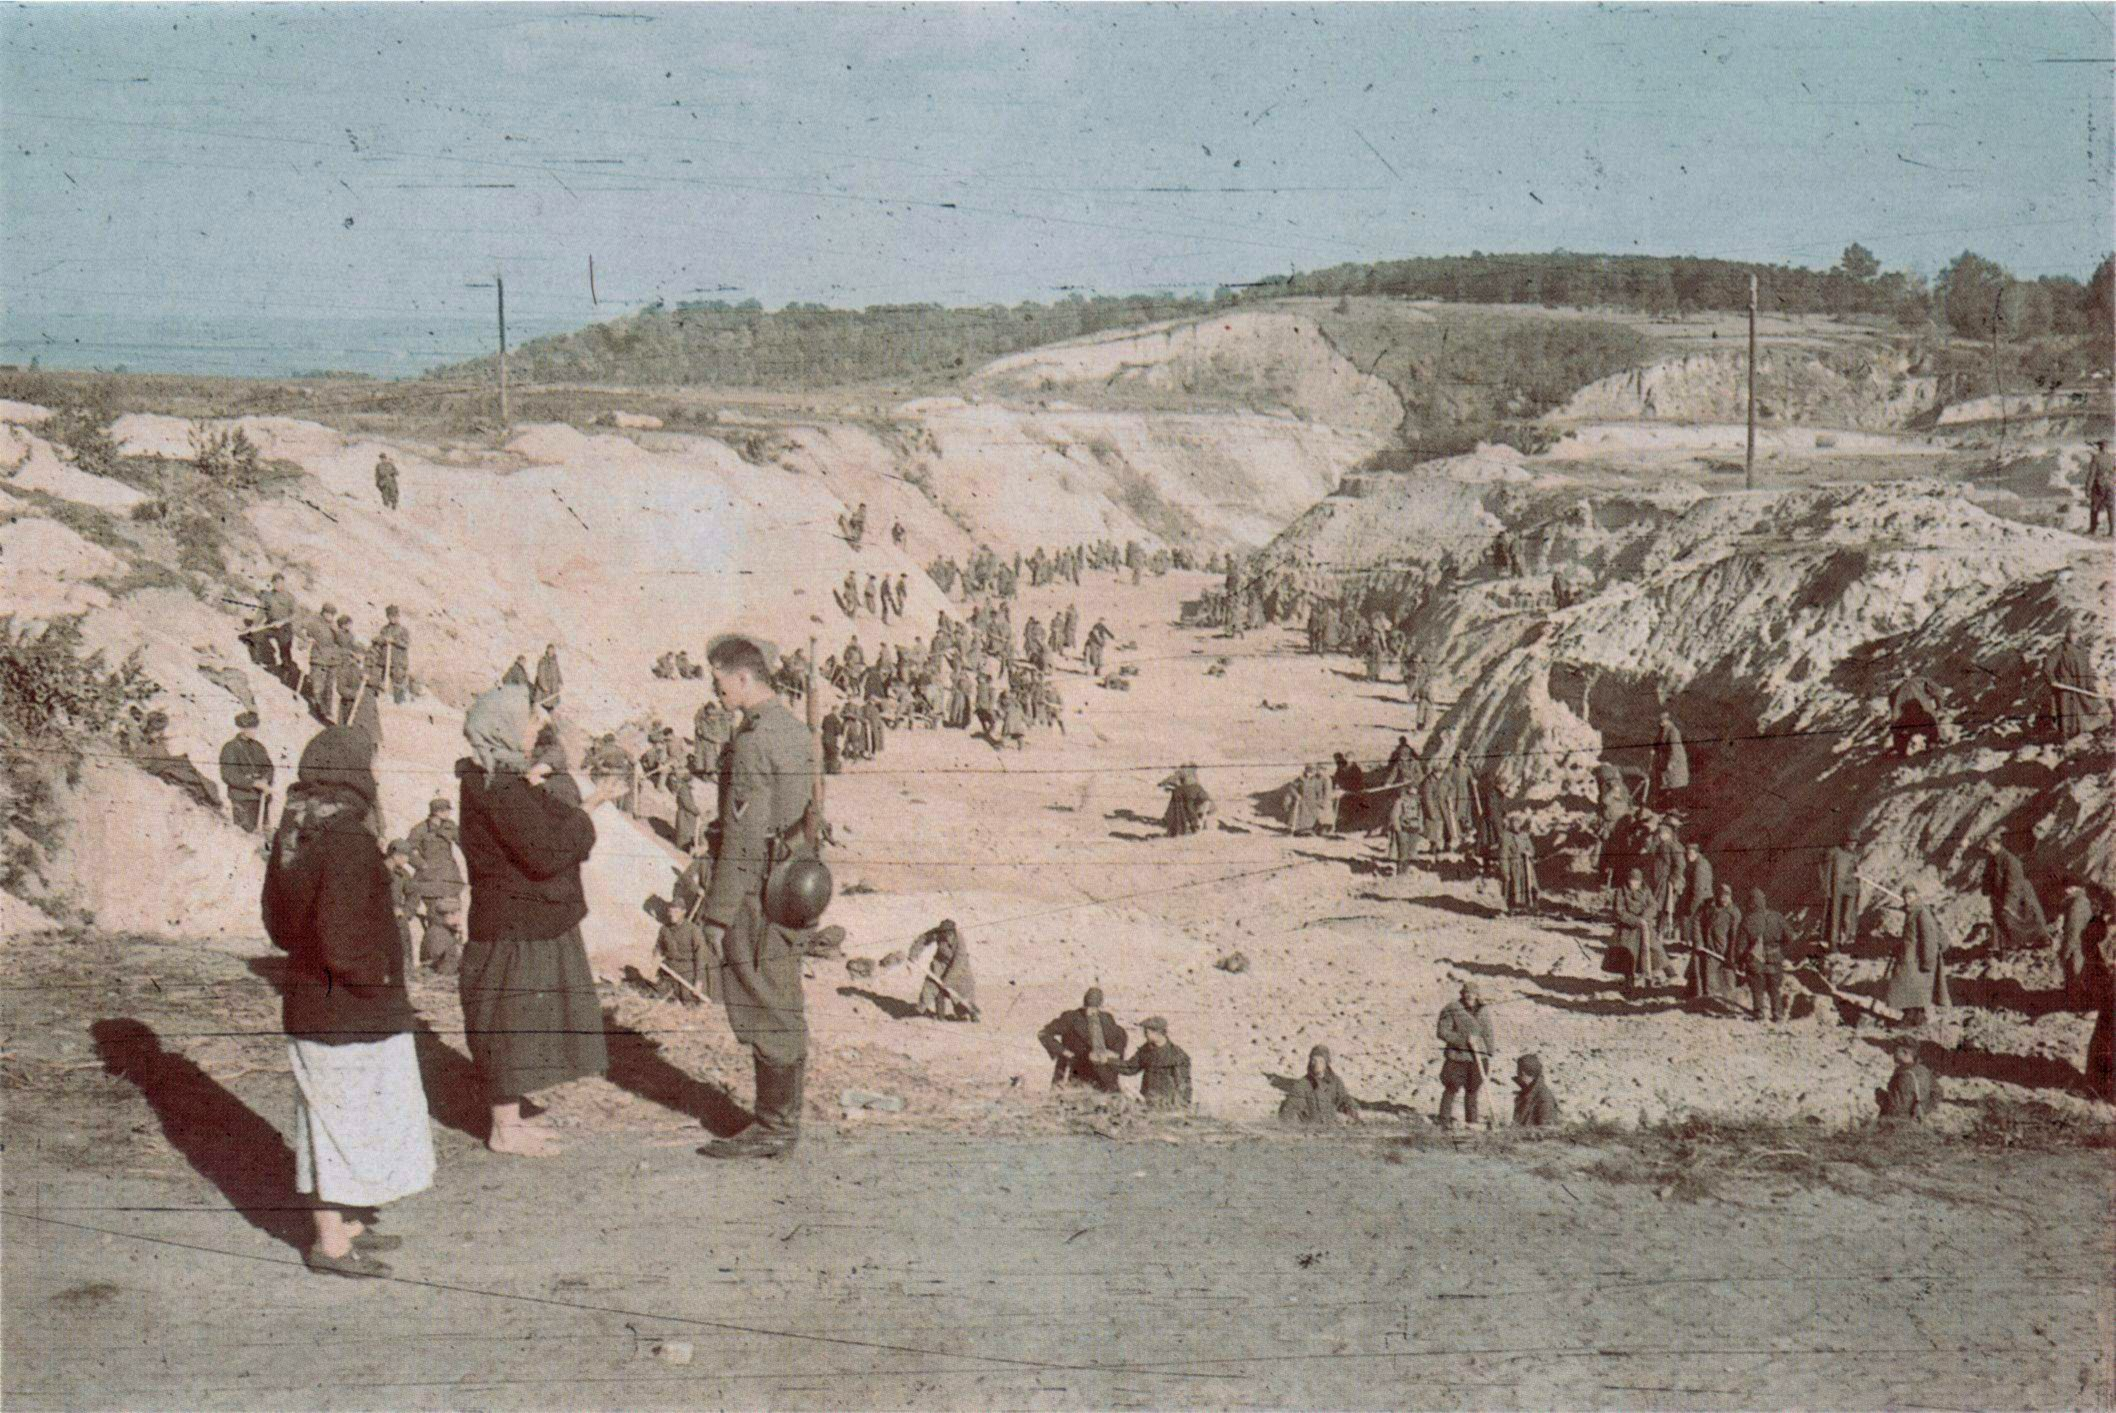
\includegraphics[width=\linewidth]{chast-zmiy/kurilo/byar-01.jpg}
\end{center}

\begin{center}
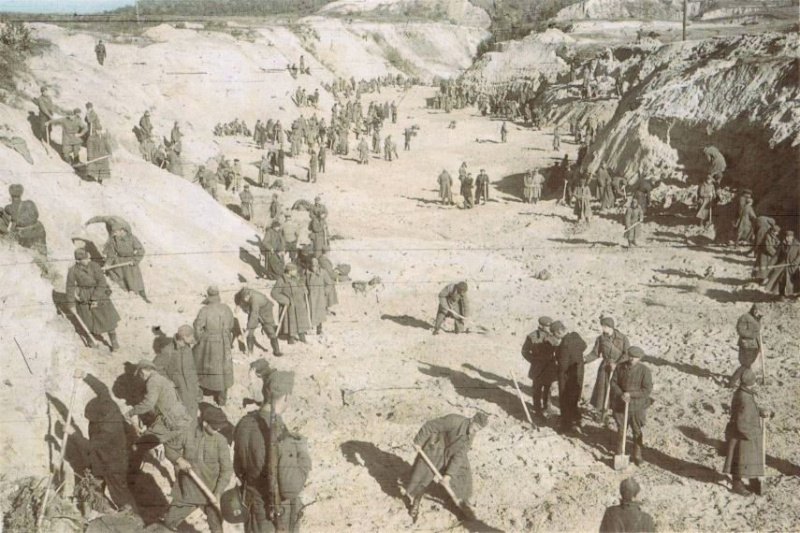
\includegraphics[width=\linewidth]{chast-zmiy/kurilo/byar-02.jpg}
\end{center}

До войны Бабий яр считался одним из наибольших киевских оврагов. Глубина его достигала 50 метров, а длина приближалась к трем километрам. По дну протекал Кирилловский ручей, ныне перехваченный бетонными желобами, уходящими в коллектор.

О каких-либо поселениях на берегах яра мне неизвестно, хотя соседний Репяхов яр был относительно обжит на стыке 19-20 веков. Происхождение названия Бабий яр неясно. В жалованных грамотах начала 15 века\cite{sofiasobor01} доминиканскому монастырю упомянуто на Нижнем Сырце урочище Хлопач или Пашня, прежде принадлежащее некой женщине Бисовой Бабе.

Причем в ранних грамотах описание, как мне кажется, размыто – его можно трактовать и вышеприведенным, и несколько иначе, что речь шла о двух урочищах – Хлопаче (принадлежавшем просто некой женщине) и Бисовой Бабе. В грамотах после 1411 года введено уточнение, задающее однозначную трактовку. А вот в «Записках о Киевском доминиканском монастыре» за 1634-1664 годы, генеральный проповедник в киевском доминиканском конвенте Петр Развидовский, описывая монастырские владения, упоминает отдельное урочище «Бесова баба»\cite{sbornikmat}:

%В грамоте князя Олелька Владимировича доминиканскому монастырю, 1411 года, говорится о правах на пошлины и перечисляются монастырские владения, жалованные Владимиром Ольгердовичем и Витовтом:

%\begin{quotation}
%Nos autem, his visis seu consideratis, dictam donationem vel eleemosynam patris Nostri iam dicti duximus confirmandam, praesentibusque confirmamus: velut theloneum, vulgo Poklodne, ut ex antiquo tenuerunt et recipiebant, villamque in ulteriori Syrecz sita, et allodium, dictum Chlopacz vel Paschnia, quae bona fuerunt cuiusdam foeminae, dictae Biesowa baba, cum omni jure, dominio omnibusque proventibus, quicunque in dictis bonis fuerunt vel fieri possint [...]
%\end{quotation}

%Строка «et allodium, dictum Chlopacz vel Paschnia, quae bona fuerunt cuiusdam foeminae, dictae Biesowa baba, cum omni jure» насколько я разбираю латынь, трактуется двояко. Первое – «Хлопач или Пашня, принадлежавшая некоторой женщине, называемой Бисова Баба, со всеми правами». Второе – «Хлопач или Пашня, принадлежавшая некоторой женщине, Бисова Баба, со всеми правами».

%Речь идет либо о Хлопаче (Пашне), что некогда была собственностью Бисовой Бабы, либо о двух отдельных урочищах – Хлопаче и Бисовой бабе.

%Praeterea villam na Zadnim Siercu cum praedio in terra dicta Chlopacz, quae bona quondam fuerunt cuispiam mulieris, dictae Bieszows Baba.

%, как пишут справочники без ссылки на источник, получило свое название от стоящего тут трактира, принадлежащего некой «бабе-шинкарке». И мол, она отдала свой земельный участок Доминиканскому монастырю, в 1401 году.

%Эти сведения сомнительны по самой уже дате. Если же их сместить на пару веков вперед, тоже не катит. В земельных польско-литовских документах не писали «баба-шинкарка», а указывали конкретные имена, к тому же неясно, зачем держать шинок в яру, где нет дороги и никто не живет.

\begin{quotation}
Там же на Сырце конвентских подданых десять.

Далее следуют грунты, названные Попковцы, где издавна некогда бывала деревушка до самой нивы, названная Плоцкая. [...]

Далее едучи от сей нивы в левой стороне грунты архимандричьи (печерские), а в правой наши, деревня Берковец; половина деревни Клашторной по самую часовню, которую мы построили, а другая половина – архимандричья. Их грунты идут на две мили к Белогородку, даже до Бесовой бабы, а наши грунты идут даже до Хлопача ко Гостомлю над Ирпенем.
\end{quotation}

Что, если в ранних грамотах напутано, и Бесова баба – таки урочище? Тогда, тождественны ли Бабий Яр и Бесова баба? Если да, то поразмыслим. Бабами издавна называли идолов – каменные бабы. А тут еще дополнительное указание – «Бесовая баба». Бесами после принятия христианства именовали поганских богов. Вдобавок, многие крупные монастыри Киева возникли на священных для язычников местах. Предположим, в Бабьем яру, точнее над ним, стоял некогда идол, баба. Не на месте ли Кирилловской церкви?

Александра Шандаренко в документальной книге про немецкую оккупацию Киева «Регистраторша ЗАГСа. Из дневника киевлянки», пишет: «Бабий Яр. Длинные, глубокие, извилистые яры, где когда-то на Ивана Купалу и на зеленый праздник Троицы женщины жали серпами высокую траву». Значит, в сороковых годах века двадцатого было еще памятно это поганское действо.

В 1944-м один из участков Бабьего яра передали во временное пользование карьероуправлению Горкомхоза для добычи глины. По пятилетнему плану 1946–1950 годов, в окрестностях Бабьего яра собирались сделать парк – что осуществили много позже. 

Трагически известная заливка отрогов яра пульпой с Петровских кирпичных заводов (по трубам от Сырецкой улицы) – итог сразу двух начинаний.

Заводам надо было сбрасывать куда-то пульпу\footnote{Пульпа вскрышных пород – при разработки глиняных карьеров в пойме Сырца производилась «вскрыша» – съем больших слоев грунта над полезной глиной. Съем выполнялся способом гидромеханизации – растворении в воде и отсоса земнасосом либо земснарядом. Жижа из воды и частиц грунта и называется пульпой.}, да и  в пятидесятых возникла необходимость проложить дорогу для соединения Куренёвки с верхним плато и замыкания кольца основных магистралей, и решили, что хорошо бы Бабий яр засыпать.

%Решение об этом приняли еще в 1950-м. За подписью начальника отдела планировки и застройки Киева М. Козлова вышло решение:

%\begin{quotation}
%Отдел планировки и застройки города не возражает против замыва отрогов Большого Яра, подходящих к территории вскрыши Сырецких заводов, на полную глубину. При проектировании учесть, что вдоль низа яра, находящегося на ул. Фрунзе, должен быть обеспечен в будущем выезд, с уклоном не более 4\%. В отношении возможности засыпки верховьев Бабьего Яра будет сообщено дополнительно.
%\end{quotation}

%В дальнейшем обсуждении проекта речь пошла о заливке всех трех крупных отрогов Бабьего яра. 

В 1961 году такое надругательство над природой и памятью дало о себе знать Куренёвской трагедией. А по засыпанным участкам яра стали проводить Новоокружную магистраль. Сейчас это улица Телиги от метро «Дорогожичи» и до Кирилловской. 

Вообще некоторые считают, что весь Бабий яр засыпан и от него почти ничего не осталось. Это не так. Основная его часть сохранилась в той или иной мере. Проще всего в этом убедиться на местности, шагая улицей Телиги вдоль холма с больницей Павлова и Кирилловской церковью.

Неподалеку остановки «Музей Кирилловская церковь» окажется, что по обеим сторонам улицы – заметные горбы. Это и есть берега низовий Бабьего яра, ранее бывшего здесь много глубже. Северный склон и ныне местами достаточно крут. Он прячется за чащей, куда бомжи нанесли толстый слой мусора. Гора обросла деревьями и уменьшились оползни.

Наибольшая область основного отрога яра уцелела и находится в современном парке Бабий яр, примерно напротив Февральского переулка и остановки «Больница имени Павлова». У остановки, направо от асфальтовой дороги, что идет к больнице, сворачивает тропинка. Она поднимается на громадную, с бетонным основанием плотину поперек яра. Она сравнительно новая, не та, которую прорвало.

Спускаемся по плитам. Ими же уложена дорога по дну яра. Громадные деревья подпирают левый, южный берег, неловко пытаясь скрыть могучую, древнюю его высоту. На гребень можно выбраться обходом, и встать вровень с кронами. Страшно!

Идем дальше. Постепенно начинает повышаться дно яра – не знаю, так ли было раньше. Всё здесь пронизано системой водоотвода. Она собирает ливневые потоки да многочисленные ручьи от родников. По бетонным желобам вода следует в общий коллектор. Ручьи на любой вкус и цвет – прозрачные, красно-бурые, обильные, полувысохшие. Вода движется, желоба соединяются. Остались и естественные русла.

Кое-где можно подобраться ко склону, есть лёссовые обрывы того масштаба, каков виден на фотографии Кирилловской стоянки, снятой Хвойкой. У подножия одной такой суглинной стены – болотце и ручей, вид совершенно первобытный.

Если пройти в направлении психиатрической больницы, будет длиться желоб с водой, и по правую руку склон, да еще один родник, сокровенный. В нем, студеном и чистом, плавает червь.

\begin{center}
\includegraphics[width=\linewidth]{chast-zmiy/kurilo/\myimgprefix byar-IMG_20140712_143446.jpg}

\textit{Улица Телиги, справа – остатки северного склона яра. 2014 год.}
\end{center}


\begin{center}
\includegraphics[width=0.96\linewidth]{chast-zmiy/kurilo/\myimgprefix byar-IMG_20140712_143940.jpg}

\textit{Вид с плотины. 2014 год.}
\end{center}

\begin{center}
\includegraphics[width=0.96\linewidth]{chast-zmiy/kurilo/\myimgprefix byar-IMG_20140712_144120.jpg}

\textit{Дорожка по яру. 2014 год.}
\end{center}

\begin{center}
\includegraphics[width=\linewidth]{chast-zmiy/kurilo/\myimgprefix byar-IMG_20140712_144453.jpg}

\textit{Часть системы водоотвода. 2014 год.}
\end{center}


\begin{center}
\includegraphics[width=\linewidth]{chast-zmiy/kurilo/\myimgprefix byar-IMG_20140712_144504.jpg}

\textit{Сплошной многометровый лёсс. 2014 год.}
\end{center}

\begin{center}
\includegraphics[width=0.95\linewidth]{chast-zmiy/kurilo/\myimgprefix byar-IMG_20140712_144545.jpg}

\textit{Источник под склоном. 2014 год.}
\end{center}

В 1960-х, в окрестностях, на улице Мельникова (бывшей Дорогожицкой) уничтожили кладбища – на месте Караимского и Старо-еврейского выстроили телецентр и спорткомплекс ДСО «Авангард», а на старой части Братского кладбища поставили телебашню. С краю отрога Репяхового яра остался кусочек Еврейского кладбища, и много надгробий сброшены в овраг под ним. Не знаю уж когда исчезло кладбище, которое было через яр напротив Кирилловской церкви, в прямоугольнике между улицами Захаровской, Петропавловской (бывший Петровский переулок) и Телиги.

В начале семидесятых на остатках верховий и середины Бабьего яра разбили парк, куда теперь обычно добираются через станцию метро «Дорогожичи». Двигаясь оттуда на северо-восток, мы попадаем в Кирилловскую рощу, предшествующую территории бывшего Кирилловского монастыря, а ныне психиатрической больницы имени Павлова, или Павловки. В этой роще, ранее – Кирилловском кладбище – встречаются могильные камни, здесь же у дороги стоит изуродованный склеп братьев Качковских, один из которых был известным в городе врачом. Тут покоились «доктор медицины Петр Эразмович Качковский и студент юрист Антон Эразмович Качковский». Покоились в прошлом, ибо тела давно исчезли, а подземные камеры наполнены мусором.

Добротно мощеная камнем дорога через чащу приводит нас к первым корпусам больницы. Южнее – недостроенное здание Института социальной и судебной психиатрии и наркологии, в народе Дурка. Тут всегда можно встретить неформалов, скалолазов и просто подозрительных типов. А севернее этой заброшки – огражденный не хуже концлагеря Городской центр судебно-психиатри\-ческой экспертизы. Его ворота имеют особенность, под ними огромный зазор.

Далее на восток, уже корпуса самой больницы и хозяйственные постройки – пищеблок, поликлиника, зал для проведения разных мероприятий. Многие стены разрисованы замечательными граффити. Домик с солнечной батареей, и рядом, на постаменте – покрытый серебрянкой бюст усатобородатого вивисектора академика Павлова. 

%Общество считает нормой одно, а ненормальным – другое, и носителей «ненормальности» стремится вернуть в лоно общепринятого движения мыслей, вроде – а давайте потратим столько-то миллиардов на вооружение, ведь убивать это самый простой и быстрый способ решения спора. Это норма. Чудака же, беседующего на улице с самим собой, называют безумцем, ставят ему диагноз и выписывают порошки. На-тко, лечись! Считай атомную бомбу нормой.

От былого монастыря, упраздненного задолго еще до революции 1917 года, осталось не так уж много – по большому счету сама Кирилловская церковь, да остатки стены середины 18 века, с башней-куполом. Стена принадлежит времени, когда архитектор Григорович-Барский выстроил тут несколько зданий. К более поздней, но все же дореволюционной старине относятся некоторые действующие корпуса больницы и одноэтажная бывшая прачечная, 1823 года, оформленная под дома бюргеров в баварских городках – ныне это корпус 10, морг, «Патанатомия». Она стоит неподалеку от церкви на север, рядом с лестницей, что спускается к улице Телиги. Прежний же старинный морг с часовней, постройки 1902 года, вероятно сооруженный на месте давней трапезной, ныне стал трапезным храмом Святителя Василия Великого.


Кирилловской церкви коснусь подробнее. Не будем забывать, что Хвойка обозначил на своей карте (смотрите главу про Кирилловскую стоянку) две пещеры – одну возле северо-западного угла церкви, другую – неподалеку, на склоне в сторону Кирилловской улицы.


\begin{center}
\includegraphics[width=\linewidth]{chast-zmiy/kurilo/Solncev_Kirilovskii_monastir_vozle_sela_Kyrenevka.jpg}

\textit{Федор Солнцев. Кирилловский монастырь возле села Куреневка. Акварель. 1843.}
\end{center}

\begin{center}
\includegraphics[width=0.60\linewidth]{chast-zmiy/kurilo/\myimgprefix kyr-cerk-IMG_20140712_142911.jpg}

\textit{Вход на территорию церкви платный. Плата не идет на пользу состоянию здания. 2014 год.}
\end{center}

\newpage
\vspace*{\fill}
\begin{center}
\includegraphics[width=\linewidth]{chast-zmiy/kurilo/kyr-kolo.jpg}

\textit{Колокольня архитектора Григоровича-Барского, простоявшая по 1937 год.}
\end{center}
\vspace*{\fill}
\newpage

Что тут было до монастыря? 

В книге Брайчевского «Когда и как возник Киев» 1964 года приводятся, со ссылкой на В. Д. Дяденко, следующие краткие сведения:

\begin{quotation}
Остатки городища чернолесской эпохи открыты на территории больницы им. Павлова [...]. Оказывается, древнерусское городище (к которому относится и сохранившаяся до наших дней Кирилловская церковь) возникло на месте более древнего городища начала раннежелезного века. В 1959 г. здесь при земляных работах были обнаружены следы жилищ полуземляночного типа; найдены обломки характерной керамики чернолесского типа, а также – фрагменты каменных зернотерок. Культурный слой, в частности, был обнаружен и под фундаментами Кирилловской церкви.
\end{quotation}

Кто возвел церковь?

В давнее время, церковь эта существовала не сама по себе, а в составе одноименного монастыря. Максимович посвятил ей статью «О создании киевской церкви св. Кирилла», где собрал доступные сведения и пришел к выводу, что церковь построена была княгиней «Марией Мстиславной, женой Всеволода Ольговича, дочерью Мстислава великого, внука Владимира Мономаха», что согласуется с летописью.

Закревский тоже приводит цитаты, и по ним получается, что монастырь основал Всеволод, отец Святослава.

Максим Берлинский, зная об упоминаниях монастыря в летописи, вразрез с нею предположил, что монастырь так назван по имени некоего Кирила, который способствовал восстановлению монастыря после «неистовства Батыева». При этом, полагал Берлинский, Кирил победил в окрестном лесу шайку разбойников, что и стало основанием легенды о Кириле Кожемяке и змие, «коего пещеры и теперь в лесу видны». Тоже подкованный в летописях, Закревский в дополнение кратко приводит содержание легенды, где Кирило Кожемяка сражается со змеем, побеждает его и в память о победе своей строит монастырь, «названный по его имени Кирилловским». Закревский также сообщает о множестве «Кирилловских пещер» и соотносит легенду о Змие с одной из них. Оставим же вопрос возникновения монастыря и церкви открытым.

%Вообще первое упоминание о Кирилловском монастыре в летописи таково, за год 1171:

%\begin{quotation}
%Сняшася братья Вышогороде и пришедше сташа на Дорогожичи под святым Кюрилом.
%\end{quotation}

%Теперь про Дорогожичи. Есть в Лаврентьевском да Ипатьевском списках за, по принятой датировке, 980 (6488) год:

%\begin{quotation}
%Стояше Володимер обрывся\footnote{Выкопал там защитный ров.} на Дорогожичи, межю Дорогожичем и Капичем, и есть ров и до сего дне.\end{quotation}

%Обратим внимание на уточнение – между Дорогожичем и Капичем. Капич – то же, что капище. Несколько позже, за 1146, читаем в Ипатьевской летописи:

%\begin{quotation}
%ту побеже Игорь и Святослав в слудовы Дорогожьчьския [...] и вбеже Игорь во болото Дорогожичьское и угрязе под ним конь
%\end{quotation}

%И за 1161 год такое описание:

%\begin{quotation}
%Перебредше Днепр, у боженки, и пойде полки к Киеву, и пришеди ста на Болоньи в лозах, противу Дорогожичу, иде к Подолью, а Ростислав стояше подле столпье (бревенчатой ограды); загорожено бо бяше тогда столпием от Горы, олы и до Днепра.
%\end{quotation}

%«У боженки» что значит? Боженка – божница, капище. А на каком берегу, левом или правом? Не сказано. Днепр перебрели у боженки. Брод там был. Брод, бродить, брести, перебрести – один корень. И перейдя через брод можно было, двинувшись в сторону Киева, добраться до Болонья-Оболони, и стать напротив Дорогожичей. Сие дает основание полагать, что тогда в пределы Дорогожичей люди включали и холм, на котором стоял Кирилловский монастырь.

%А боженка и Капич – одно ли урочище? Одно, если боженка – на правом берегу. Капич – точно на правом. Раз Капич и Дорогожичи – смежные, а боженка и Дорогожичи тоже смежные, значит боженка равняется Капичу. Ежели это справедливо, то Капичем, боженкой, некое место у Днепра близ переправы слыло по меньшей мере 1161 летописный год.

%Если же Боженка – на левом берегу, получается, что Капич – отдельное урочище близ Дорогожичей, и Боженка к Капичу не относится. В таком случае Капичем мог называться Бабий яр, где, как я предполагаю, на холме стоял идол, «баба».

Долгое время монастырь занимал всю местность, где теперь корпуса психиатрической больницы и церковь. В конце 18 века у монастыря отобрали земли, а затем и сам монастырь был упразднен, осталась только церковь, трапезная да колокольня (снесли в 1936 – помешала!), а в остальных зданиях поместились Кирилловские богоугодные заведения, где еще тогда, кроме прочего, устроили больницу «для умалишенных». Из нее и выросла, в 1920-30 годах, пресловутая психушка Павловка. 

Что же было на месте холма, когда там не стоял «святой Кюрила»? Помимо краткого сообщения Брайчевского про «остатки городища чернолесской эпохи», от которых ни холодно, ни жарко, сведений мало.

Там где на холме, будто крепкий гриб, растет сама церковь, была одна или несколько пещер, а скорее – целая сеть подземных ходов, пронизывающих гору.

Сементовский в 1864 году полагал, что у истоков Кирилловского монастыря стояли отшельники, обитавшие в пещерах. Дескать, в конце 11 или начале 12 века инок Кирилл вырыл там «пещерную келию». Закревский считал это выдумкой Сементовского.

%В конце 1880-х где-то около храма провалилась земля и открылся подземный ход. Туда проник служитель церкви Кулиш и увидел гробы в нишах, перпендикулярных коридору. Позже лаз в пещеру был засыпан.

Газета «Киевлянин» в нумере 238, 1909 года, напечатала статью Л. Зимина «Кирилловская обитель», откуда выпишу всё важное, опуская общеизвестные сведения про историю церкви и тому подобное.

По ходу будем разбирать прочитанное.

\begin{quotation}
В субботу, 15 августа, архитектор Д. В. Милеев, под наблюдением которого проводятся археологические раскопки в усадьбе Десятинной церкви, супруга его, большая любительница археологии, прив. доц. В. Г. Ляскоронский, подполковники Б. С. Стеллецкий и М. К. Дитрихс и автор настоящей заметки совершили поездку для исследования обнаруженной возле Кирилловской церкви пещеры с погребениями да кстати лишний раз осмотреть и самую церковь.

Кирилловские богоугодные заведения находятся на краю города на отдельном холме, который одним оврагом\footnote{Репяхов яр.} отделяется от Киева, другим\footnote{Бабий яр.} от Копылова.

Лукьяновско-Кирилловская линия трамвая чуть ли не самая интересная в Киеве. С нагорной ее части открываются широкие и живописные виды, особенно на долину Днепра; большая же часть линии пролегает по склону большого оврага\footnote{Репяхов яр.}, так что с одной стороны вы видите крутой откос горы с жалкими хатами наверху, а другой обрывистый склон оврага, сильно разветвляющегося и далеко вдающегося в гору; по дну оврага, по зеленому бархатному ковру течет довольно большой ручей, к которому в разных местах присоединяются меньшие.

В одном месте трамвай проходит через небо\-льшое ущелье.

В горах кое-где чернеют пещеры; одна из них очень просторная, эти пещеры мы пока еще не осматривали.
\end{quotation} 

Пещеры! Где же именно они были, как и когда сгинули? «Кое-где» мало что проясняет.

Зимин описывает поездку на трамвае, и это дает зацепку, что речь может идти только о той части Репяхова яра, по которой проходил маршрут – склон южного отрога и лежащий к северу от него отрезок яра, где оба отрога, составляющие этот громадный овраг, уже соединились у развилки при остром клинообразном мысе.

Серпантин дороги вдоль берега яра, трамвай да ручей – известный вид на дореволюционных открытках. Современные краеведы окрестили это место «Киевской Швейцарией», а книги и статьи переполнены ошибочными сведениями о том, что трамвай шел по улице Макаровской.

На деле же трамваи маршрутов 18 и 20 ходили непосредственно в яру (нисходя в него), под Макаровской, что на западном гребне отрога Репяхова яра. Маршрут 18-го трамвая, в некотором переложении на современность, был таким: нынешний сквер с фундаментом церкви св. Федора (на пересечении Овручской с Багговутовской) – Овручская – Нагорная (Подольского спуска не было), затем по Врубелевскому (тогда Макаровскому) спуску в Репяхов Яр до Кирилловской площади, и назад по яру же и через Пугачева да Багговутовскую обратно к церкви св. Федора. С течением времени маршрут несколько менялся, но первоначальный был именно таков.

Ручей в яру сохранялся до 1950-х, в нем даже водилась мелкая рыба. На одном из склонов местные жители помнят несколько пещер, а про семидесятые годы рассказывают, что в конце Ново-Макаровской улицы, на пригорке обитал отшельник, старик. Он выстроил себе приземистую хижину из бревен и разводил пчел.


%А в 1913 году существовал еще длиннющий маршрут 20, от Думской площади («Майдан»), по Большой Житомирской, Дорогожицкой, Овручской, затем повторявший часть 18-го и следующий еще далее Куренёвкой по улице Кирилловской.

%r03.jpg
%r04.jpg

%r01.jpg

%r07.jpg
%r08.jpg

\vspace*{\fill}

\begin{center}
\includegraphics[width=0.90\textwidth]{chast-zmiy/kurilo/s-r09.jpg}

\textit{Вид снизу вверх, Кирилловская церковь позади фотографа справа.}
\end{center}

\vspace*{\fill}


\begin{center}
\includegraphics[width=\linewidth]{chast-zmiy/kurilo/s-r02.jpg}

\textit{Вид сверху вниз, в сторону Кирилловской церкви с колокольней. Дореволюционная открытка.}
\end{center}

\vspace*{\fill}

\begin{center}
\includegraphics[width=\linewidth]{chast-zmiy/kurilo/s-r05.jpg}

\textit{Старинный снимок сделан в самом яру.}
\end{center}

\vspace*{\fill}


%\begin{center}
%\includegraphics[width=\linewidth]{chast-zmiy/kurilo/s-r06.jpg}

%\textit{И сей тоже.}
%\end{center}
%\vspace*{\fill}

\begin{center}
\includegraphics[width=\linewidth]{chast-zmiy/kurilo/rep-14.jpg}

\textit{Дореволюционный снимок. Трамвай еще не ходит.}
\end{center}

Всё то, что показано на открытках и фотографиях, нынче выглядит совсем иначе. Часть Репяхового яра занимают бесконечные гаражные кооперативы, их остатки да подобные проявления человеческой цивилизации. С ними можно познакомиться, спускаясь по выморочной Макаровской улице и левее, левее. Отовсюду торчат бетонные, кирпичные фундаменты, ржавая арматура, в земле зияют провалы, и всё это буйно заросло деревьями, бурьяном и щедро украшено россыпями битого стекла – ах, как блестит оно на солнце!

Вдоль Макаровской в сторону Репяхового яра отделяется дорога с красивым названием – Врубелевский спуск. Между гаражей и замусоренных склонов, дальше уводит он в места, где и днем всюду чудятся разбойники. Это здесь были проложены трамвайные пути. На некоторых отрезках спуск совсем непроходим – надо лезть в обход или перебираться по краешку обвала.

Вдоль южного отрога Репяхового яра, Врубелевский спуск нисходит по зарослям репейника ко дну самого яра чуть восточнее места соединения двух главных, громадных оврагов, составляющих Репяхов яр в виде упавшей на левый бок, искореженной буквы «Y».

\begin{center}
\includegraphics[width=\linewidth]{chast-zmiy/kurilo/\myimgprefix IMG_20130915_143657.jpg}

\textit{2013. Начало Врубелевского спуска, наверху.}
\end{center}

По каждому из них протекает ручей. Как и овраги, оба ручья сходятся и далее текут уже вместе. Так было прежде, до вмешательства человека. Ныне часть вод загнана в пахнущий химией коллектор, а часть протекает поверхностью – у обочины и просто дор\'огой, вымощенной бетонными плитами от стройки, что ведется в дальней части одного из приярков. На плиты ручьем намыло богатую железными частицами, буроватую глину, в которой завелись микроскопические водоросли. Дорога пахнет морской капустой или речными водорослями, которые вытащены на сушу и сохнут в песке.

%На этой фотографии запечатлено место, откуда трамвай по террасе спускался в яр:

%\begin{center}
%\includegraphics[width=\linewidth]{chast-zmiy/kurilo/\myimgprefix IMG_20130915_144450.jpg}
%\end{center}

%\newpage

%И пара снимков 2013 года, уже на дне яра:

%\begin{center}
%\includegraphics[width=0.95\linewidth]{chast-zmiy/kurilo/\myimgprefix rep-05.jpg}
%\end{center}

%\begin{center}
%\includegraphics[width=0.95\linewidth]{chast-zmiy/kurilo/\myimgprefix rep-08.jpg}
%\end{center}

%\newpage


\begin{center}
\includegraphics[width=\linewidth]{chast-zmiy/kurilo/\myimgprefix IMG_20130915_144633.jpg}

\textit{2013. Дорога на дне яра.}
\end{center}

Со склонов сочатся ручейки и бегут между зарослей репейника. У обочины встречаются наполненные водой ямы, где видно относительно крупные водоросли, похожие на хвойные ветки. По склонам яра стоят, подпирая небо, громадные деревья – ивы с толстенными стволами, серебристые тополя. Некоторые деревья увиты лианами.

Сами склоны рассмотреть зачастую трудно из-за зелени, мокроты и нагромождений живых и сломанных деревьев. От голых склонов с фотографий 19 века не осталось и следа.

Такова местность, описанная Зиминым, сейчас. Продолжим читать его статью.

\begin{quotation}
В церковь мы прибыли в одиннадцатом часу утра; несмотря на большой праздник, молящихся было очень немного, да и те, судя по одежде, из больницы и богадельни. Находясь в мало населенной местности и не имея прихода, Кирилловская церковь является как бы домовой церковью при Кирилловских богоугодных заведениях и вместе с ними состоят в ведении Киевского губернского земства.
%\end{quotation}

%\begin{center}
%\includegraphics[width=\linewidth]{chast-zmiy/kurilo/\myimgprefix vidkyr.jpg}

%\textit{Дореволюционный снимок. Вид на Кирилловскую церковь со стороны низовья Бабьего яра, там где перекресток Кирилловской и Телиги.}
%\end{center}

%\begin{quotation}
Настоятель церкви был занят, единственный из служащих, видевших пещеру и погребения, некий Кулиш, ушел на курёневскую ярмарку, а смотритель зданий мог только приблизительно указать то место на склоне горы, где должен быть вход в пещеру.

Подполковник Дитрихс и я спустились и тщательно осмотрели весь склон у подошвы горы; нашли множество нор, из которых две своими размерами особенно привлекли наше внимание; пещеры же не нашли.

Смотритель послал разыскать Кулиша; мы же, ожидая его возвращения и окончания службы, расположились на травке под стеною храма, беседуя как о самом Кирилловском храме, так и о других памятниках старины. [...]

Последний раз Кирилловская церковь упоминается в летописи под 1231 годом, а затем до 1555 г. о ней нет никаких сведений. [...]

%Батый, разгромив Киев, почему-то не тронул Кирилловской церкви.

В 1555 году Сигизмунд II отдал Кирилловскую церковь со всеми имуществами, которые ей принадлежат, некоему Шавуле, предоставив ему те же права по отношению к церкви, какими пользовались его предки; в 1565 году имущества упраздненной Кирилловской церкви приписаны к Никольской церкви, которая находилась в киевском замке. [...]

И только в 1605 году известный ревнитель православия князь Острожский поручил игумену Острожского монастыря св. Креста Василию Красовскому восстановить Кирилловский монастырь и возвратить все имущества [...]

Кулиш с ярмарки не возвращался; терпение наше истощалось, и мы уже все компанией принялись за новые поиски\footnote{Давно пора, чем Кулиша ждать.}. Вышеупомянутые норы оказались ниже того уровня, где возможно было бы существование пещер; но там, где это возможно, ни нор, ни каких-либо иных признаков существования пещер не оказалось.

Нашли несколько кирпичей XVII века, вероятно обломки стены, часть которой сохранилась до сих пор, а часть, шедшая по краю горы, разрушена; фундамент ея в некоторых местах выступает наружу.

Мы еще не закончили своих поисков, как нас пригласили к священнику. Он указал нам на краю горы, шагах в 45 к северу от храма место, где стояла часовня; возле нея, ближе к храму, находился морг, т.е. ледник для хранения мертвецов, а возле него образовался какой-то провал, в котором и обнаружена была пещера.

Кулиш проник в эту пещеру и по сторонам видел гробы в нишах, лежащие не вдоль пещерного хода, как в лавре, а перпендикулярно к нему. Кулиш прошел несколько сажен по направлению, как он думает, к северному входу в храм и, увидав толстые скрещенные балки, дальше идти не решился.

Было это лет двадцать тому назад, но до сих пор никто не счел нужным исследовать эту пещеру, и только теперь Б. С. Стеллецкий, прослышав о ней, организовал компанию для археологической разведки.

От часовни не осталось и следа, морг и провал засыпаны; все место сравнено с остальной площадью, на которой стоит храм; кроме того тут идет систематическая свалка для дальнейшего расширения площади.

Для того, чтобы на склоне горы открыть вход в пещеру, пришлось бы снять большой пласт и на довольно большом пространстве, так как точно место входа осталось неизвестным.

Поэтому решили сделать траншейку на пути от бывшего провала к северному входу в храм; траншейка, конечно, должна пересечь пещерный ход. Поручив это дело опытному рабочему, которого захватил с собой Д. В. Милеев\footnote{Рыть сообща было бы скорей, белоручки.}, мы тем временем решили осмотреть храм.

Пока ходили за ключами, священник указал нам место, где находилась трапезная церковь во имя св. Василия – это шагах в 40 к западу от храма; там сейчас клумба цветов. Священник говорит, что пол бывшего алтаря остался нетронутым; возможно что под престолом, как это обыкновенно делается, заложена ценная святыня.

Вокруг Кирилловской церкви было когда-то кладбище; один из надгробных камней еще и теперь лежит сверху; остальные, по словам священника, зарыты вдоль северной стены храма.

Проходя по этому месту, мы невольно обратили внимание на двери северного входа; в них щели пальца в два шириной, нижняя доска совсем вывалилась; в таком же состоянии оказались южныя двери; [...] 

Тем временем во дворе уже вырыта была траншейка, и некоторое время думали даже, что попали как раз на погребение; однако это не подтвердилось, и прощупывание почвы длинным железным стержнем тоже не давало никаких результатов.

Наконец, явился Кулиш и, по его рассказу оказалось, что траншею следовало рыть немного левее\footnote{Следовало дождаться Кулиша и тогда уже рыть траншею.}. Начинать новую траншею было уже поздно; пришлось поиски пещеры отложить до другого раза [...]
\end{quotation}

Компания посетила трехярусную колокольню 1748 года строения, третий этаж которой был поначалу деревянным, но сгорел в 1849 году, и его возобновили каменным.

\begin{quotation}
По обе стороны главного корпуса колокольни имеются пристройки; в одной из них находится лестница; сначала она широкая, заполняет всю пристройку, а выше заменяется двумя; одна ведет во второй ярус, где теперь помещается аптека Кирилловской больницы; другая тоже во второй ярус, в верхнюю часть его – на потолок больницы\footnote{Далее в статье речь идет о потолке аптеки, таким образом второй ярус был разделен на два этажа, один с аптекой, другой – помещение над нею.}. Над входом в помещение аптеки имеется чугунная доска с надписью, свидетельствующая о том, что в 1760 году игуменом Феофаном Желтовским здесь была устроена церковь во имя Благовещенья. [...]

На третий ярус ведет узкая каменная лестница, заключающаяся внутри стены. Пол третьего яруса страшно ветхий, в одном месте и притом как раз около колоколов большая дыра; говорят, что зимой здесь бывает по колено снегу, который, конечно, забивается под пол на свод второго яруса, где потом тает, проводя сырость [...]

Есть еще деревянная лестница на самый верх колокольни, но смотритель не советовал взбираться туда, вследствие ветхости и лестницы, и помоста. 

Колоколов немного и самый большой из них очень невелик; видно, что колокольня рассчитана на гораздо большую тяжесть.
\end{quotation}

Затем любители старины отправились исследовать некую пещеру неподалеку:

\begin{quotation}
Осмотрев колокольню, пошли к пещере, находящейся, за кладбищем версты за полторы от церкви\footnote{Около 1,6 км.}.

На вершине высокого мыса, называемого местными жителями Курганом, находится довольно большая яма, а в ней нора, сразу уходящая вниз на неизвестную глубину; 

в нескольких шагах от нея на склоне горы другая таких же размеров, но уходящая в гору горизонтально; с другой стороны Кургана еще одна, широкая, просторная.

Так как забираться в пещеры без огня не было никакого смысла, то послали в лагери\footnote{Вероятно, военные лагеря, между речкой Сырец и верховьем Бабьего яра. Окрестности улицы Вавилона и примыкающего к ней отрезка Щусева. Туда можно добраться как от Репяхового, так и Бабьего яров. Думаю, от Кургана до лагерей было ближе, чем к Кирилловской церкви, раз послали за свечами в лагеря.} за свечами, а тем временем Д. В. Милеев, подполковник Дитрихс и я, в сопровождении сторожа, спустились на дно оврага, где протекает довольно большой ручей; почти на каждом шагу встречаются родники; один из них, появившийся только в этом году, довольно большой; вода этого родника чистая, холодная, с сильными минеральными примесями.

Ручей, размывая почву, обнажил толстый пласт дерева; в некоторых местах сохранилось слоистое строение, и там, где пласт особенно подвержен влиянию воды, слои легко отделяются друг от друга; в иных же местах попадаются уже не слоистые, а однообразные строения куска (угля) с ясными, однако, следами сучьев.

Мы захватили образцы для того, чтобы показать специалистам по ботанике и геологии, не имеем ли мы дело с остатками первобытных лесов.

Когда мы поднялись из оврага, были принесены уже и свеча, и лампа.

Большая пещера особого интереса не представила; будучи освещена внутри, она вся видна от входа; никаких ходов в стороны нет; свод в ней сырой; очевидно над ней находится водоносный слой.

Другая пещера оказалась интереснее. Пробраться в нее можно только ползком, но в неско\-льких шагах от входа она уже так высока, что рукой нельзя достать ея свода.

Кроме того, подполковник Дитрихс прошел по ней прямо тридцать шагов, повернул налево, прошел еще 19 шагов. Дальше пещера поднимается, но сама становится ниже; по-видимому, она имеет другой выход, как так ощущается небольшой сквозняк, но вместе с тем лампа сильно портит воздух; 

опасаясь возможности взрыва, подполковник Дитрихс вернулся назад, решив в один из ближайших праздничных дней исследовать пещеру до конца с электрическом фонарем.

Пещера, по-видимому, посещается, так как стены ея исписаны, но подписей подполковник Дитрихс не разобрал. Говорят, что здесь искали клад. [...]

Третью нору не исследовали, так как стало темнеть. Следующая разведка должна дать более интересные результаты, так как займемся исключительно пещерами и исследуем их до конца.
\end{quotation}

В номере 248 за 1909 год «Киевлянин» напечатал еще одну заметку про Кирилловскую церковь и находящиеся рядом пещеры. Почитаем.

\begin{quotation}
Внимание комиссии\footnote{Ее состав: Б. С. Стеллецкий, Дитрихс, Ляскоронский, Д. В. Милеев.} обратила на себя находящаяся у северной стены древней церкви пещера, о которой раньше археологи не знали. 

Было известно о существовании пещеры на южной стороне холма, на котором расположена церковь. Лет 30 тому назад на этом месте образовался провал и один смельчак задумал спуститься в пещеру, в которой предполагались сокровища. Смельчак, спустившийся по веревке, за которую держались несколько человек, своего предприятия не довел до конца в виду огромной глубины. Исследованием новооткрытой пещеры и думает заняться комиссия\footnote{Идет ссылка на Киевские Вести 19 августа, номер 220 и Спб. Ведомости 23 августа, номер 188.}.
\end{quotation}

Очень неоднозначно написано. По смыслу вроде бы можно сопоставить «смельчака» со служителем церкви Кулишом из предыдущей статьи. Однако в ней не было подробностей про спуск на веревке, и Кулиш лазал в пещеру, ход куда открылся «шагах в 45 к северу» от храма, а тут речь идет про «южную сторону холма».

Прикидывая на местности, 45 шагов на север – там действительно крутой северный склон горы, с каменной лестницей за зданием бывшей прачечной, ныне морга. А южная сторона горы – метрах в двухста от церкви, склон уже Репяхового яра.

Поэтому я не понимаю, то ли написано о двух разных пещерах – северной и южной, то ли спутаны стороны света и вместо «южная сторона холма» следует читать «северная», тогда всё становится более ладным. Дескать, лет тридцать назад открылась пещера на северном склоне, на неё-то сейчас и обратили внимание археологи. 

Иначе придется предположить, что была еще какая-то пещера на южном склоне, куда 30 лет назад спускался на веревке не Кулиш, а какой-то другой смельчак.

Но на карте Хвойки, которую я приводил в главе «Кирилловская стоянка», создатель ея обозначил таки две пещеры возле церкви. Одну пещеру у северной стороны церкви, другую подле, примерно, восточного угла горы, направленного к стадиону. О последней пещере все источники молчат.

Еще более примечательно, что карта Хвойки опубликована в 1899 году, а мы разбираем статьи 1909-го. И вот Зимин, Дитрихс, Стеллецкий, Ляскоронский, Милеев в первой статье разводили руками и заставляли рабочего копать в ошибочном месте, и ждали Кулиша, а у Хвойки уже за десять лет до того там указаны целых две пещеры – одна из которых, судя по всему, и есть та самая «северная».

\begin{quotation}
6 сентября члены киевского отдела Императорского военно-историческаго общества Б. С. Стеллецкий, М. К. Дитрихс, проф. В. В. Завитневич и некоторые другие лица вновь совершили поездку для исследования кирилловских пещер. Пещеру, находящуюся возле самой церкви, вследствие отсутствия архитектора Д. В. Милеева и В. В. Хвойка, не раскапывали;
\end{quotation}

«Возле самой церкви» – вероятно, речь идет о той самой «северной» пещере, куда лазал Кулик. Отметим еще, что Хвойка и Милеев не явились. Так и неясно, проводилось ли исследование пещеры в 1909 году. 

\begin{quotation}
ограничились лишь пещерой, находящейся в так называемом Кургане за Кирилловским кладбищем. Пока рабочий под наблюдением Б. С. Стеллецкого расчищал вход в пещеру, остальные члены компании спустились на дно оврага, чтобы показать проф. В. З. Завитневичу те пласты дерева и угля, о которых я недавно сообщил в «Киевлянине». Проф. Завитневич очень заинтересовался как этими пластами, так и вообще слоями почвы, которые здесь выделяются очень отчетливо, и захватил образцы для более детального исследования.

Когда вход в пещеру достаточно расчистили, М. К. Дитрихс и я, в сопровождении одного рабочего, вооружившись лопатами и электрическими фонарями, проникли в пещеру; вскоре присоединился к нам и проф. В. З. Завитневич.

Сначала идет коридор, немного лишь заворачивающийся вправо, длиною 20 3/4 арш.\footnote{14,76 метра.}; по сторонам его попадаются ниши; некоторые из них настолько велики, что в них свободно может спрятаться человек. На 20-м аршине отходит ветвь влево, тоже немного заворачивающаяся в правую сторону, а в общем составляя с первым коленом угол в 50 градусов. Все протяжение второго колена около 9 аршин\footnote{6,4 метра.}.

На шестом аршине опять влево почти под прямым углом идет новый, короткий, всего около двух аршин, ход, который приводит в небольшую овальную пещеру; из нее во второе колено коридора пробито окно, вершков 5\footnote{22 сантиметра.} в диаметре.

Коридоры настолько узки, что оба плеча трутся об их стены; высота же их крайне различная. В некоторых местах насилу достаешь потолок рукой, в иных и особенно в конце можно пробраться только ползком; не только разминуться с кем нибудь, но и самому повернуться невозможно.

Объясняется это тем, что пол пещеры – наносный или позднейшие раскапыватели, ленясь удалять землю наружу, нагребли бугры по дороге, или вода их намыла, а может быть, действовали обе причины.

Раскапывая пол пещеры, находили твердый грунт лишь на глубине аршина и более. Когда ударяли о пол в конце второго коридора, то слышался гул, указывающий на пустоту под полом. Пол в самой пещере очень мягкий и при раскапывании обнаружен, как будто, ход вниз и обратно, в роде как бы второй или, вернее, подвальный этаж коридора; гул этот можно было объяснить еще и иначе: верхний слой пола утоптан, а ниже он сравнительно, рыхлый, следовательно более пустой.

Против вышеупомянутого окна, в правой стене коридора имеется низкая, но широкая ниша, а в ней уходящий вглубь рукав, в который можно только просунуть руку; дальше он заворачивает влево; такой же рукав есть рядом с нишей и в некоторых других местах.

Когда немного раскопали нишу, то в ней оказался еще один такой рукав. Задняя стена и потолок ниши были обмазаны известью, а на дне ея глина носит следы угля; очевидно, это был очаг, а рукава служили дымовыми трубами и вообще предназначены для вентиляции. Вероятно они и сейчас имеют выход наружу, так как воздух в пещере, несмотря на продолжительное пребывание в ней трех и четырех человек, оставался свежим. Вероятно, отверстия этих отдушин засорились, так что глаз не замечает их.

Мы нашли одно отверстие, но по-видимому, отдушина засорена где-нибудь внутри, потому что ни звук, ни свет внутрь пещеры не проходят. Присутствующие наверху кургана отчетливо слышали, как копались внутри пещеры. 

На дне только что упомянутой ниши оказалось еще углубление яйцевидной формы, тоже вымазанное довольно толстым слоем извести; кроме того, тут же попадаются комочки извести, напоминающие фигурки различных животных; некоторые из них, будучи ветвисты, все же плотно приходятся друг к другу.

Пещера находится в лесе; стены, свод, а также и пол ея, где нет наносной земли, настолько прочны, что весьма нелегко поддаются саперной лопате и весьма острому железному щупу. Если удалить наносную землю, то пещера, т.е. свободное пространство в конце коридоров, окажется довольно просторной, но удалять землю надо от самого входа, что потребует много времени.

Поэтому, осмотрев по верху в соответствующем направлении коридоры и видя, что яма с новой в вершине кургана приходится над пещерой, решили проникнуть в пещеру с этой стороны, надеясь, что это будет скорее, чем прочищать все коридоры. Однако, здесь нора сразу идет вниз и, по-видимому, на большую глубину, так что потрудившись до самого вечера, мы все-таки не достигли пещеры. 

Хотя, таким образом, окончательно расследовать пещеру не удалось, но открытая ниша, вымазанная известью, с явными признаками очага, с углублением, имевшим, очевидно, какое-то специальное назначение, а также несколько запутанные ходы, окно из пещеры в коридор, – все это показывает, что пещера выкопана не простыми кладоискателями; они могли только испортить ее последующими раскопками. (Наибольшее подозрение со стороны проф. В. З. Завитневича падает на известного генерала Багговута и жену его).

План пещеры очень близко подходит к плану леваго края Дальних пещер в Лавре, если смотреть от входа в пещеры. Надписи на стенах пещеры не дают никаких сведений, которые свидетельствовали бы о времени открытия ея; впрочем, разбирать все из требует слишком много терпения и хорошего освещения\footnote{Нигде более сведений о надписях, да и о самом Кургане, я не нашел.}.

Хорошо утоптанный насыпной пол показывает, что пещера посещается давно; в одной нише найдена визитная карточка некоего Ренского. На этот раз пещера заинтересовала нас еще более, чем в предыдущий, и мы, конечно, еще вернемся к ней\footnote{Заманчиво полагать, что в «Киевлянине» есть продолжение, однако я не знаю, в каком номере его искать.}. 
\end{quotation}

Поначалу я был знаком только с последней статьей, и не знал, что в первой указано расстояние до Кургана – полторы версты. Меня начало мурыжить, как же найти этот Курган. Я стал прикидывать.

Имелись ориентиры – Кирилловское кладбище да упомянут овраг: «Пока рабочий [...] расчищал вход в пещеру, остальные члены компании спустились на дно оврага». Значит, Курган с пещерой был около края оврага, причем в таком месте, где участники экспедиции, не скалолазы, могли слезть на дно.

Вдобавок меня сбило с толку сообщение о пещере в «южной стороне холма». Не ведая о первой статье, я как один из вариантов рассматривал, что пещера, куда лазал «смельчак» – та же, которая «в Кургане», и если это так, то Курган следовало искать в Репяховом яру. Ведь Кирилловское кладбище занимало поверхность горы на запад за Кирилловским монастырем, северной стороной выходя на Бабий, а южной – Репяхов яр. 

Прежде поисков Кургана, мы просто искали пещеры в Репяховом яру. В ходе съемок «Киевской амплитуды» и мной отдельно был исследован западный склон к западу от Макаровской улицы по дорогу на дне яра, и бегло осмотрена часть противоположного склона общего отрога. Пещер мы не нашли. Сложность местности, а заодно вмешательство  человека, существенно затрудняют дело.

Краеведческая вылазка вдоль южной части холма, на котором стоит Кирилловская церковь и больница, в июле 2014 года, когда мы пытались найти «местность Курган», принесла некоторые плоды.

Пробиваясь по краю яра вдоль забора, не доходя до свалки рядом с психбольницей, эдак по координатам 50°28'48.33"N 30°28'15.68"E, мы нашли вертикальный ход в земле, метра два глубиной, уходящий потом в сторону. Спускаться без каких-либо приспособлений туда не рискнули. Я порывался, но меня отговорили, мол, можно провалиться. Земля, а точнее глина внизу была рыхлой, лежал какой-то большой кирпич или камень. Хотелось думать, что это вход в пещеру, найденный «смельчаком» (мы еще не знали о первой статье Зимина), но про ту пещеру сказано, что «открылся провал», а здесь мы столкнулись с тщательно выкопанной шахточкой, причем в месте, куда очень трудно добраться с любой стороны.

\begin{center}
\includegraphics[width=\linewidth]{chast-zmiy/kurilo/\myimgprefix rep-IMG_3887.JPG}
\end{center}

Вниз по отвесному почти склону тянулась великанская борода мусора, двигаться назад в сторону Кирилловской улицы – сложно и долгонько, путь к окраине Павловки преграждают непреодолимые кусты и забор, а если продираться дальше с большой осторожностью, попадаем на свалку.

Ход был вырыт чем-то небольшим вроде саперной лопатки, потому что большой лопатой там не размахнешься. Следов выброшенного грунта снаружи не замечено, возраст раскопа определить трудно. Если там и лежали прошлогодние листья, то их присыпало землей. Форма хода – квадрат со сглаженными углами, если я спущусь, то подняв руки, достану до краев ямы, но широко расставить руки в стороны не смогу – узко.

Неясно, как далеко идет от дна горизонтальный ход. По виду, я бы мог засунуться туда ползком на спине, ногами вперед, никак иначе.

Продвигаясь от свалки\footnote{Кстати, в конце 1930-х свалка была и где-то на улице Макаровской, а это значит, что часть склона Репяхового яра, где могли быть пещеры, оказалась засыпана еще тогда.} (где я удачно наступил на шприц и пробил через кроссовок ногу) в неопределенном направлении, мы вышли к полукруглому тупику оврага близ недостроенного здания Института социальной и судебной психиатрии и наркологии.

Там, в тупике, странное место – непонятные деревянные сооружения, на суку дерева висел череп коровы, а склоне слева темнело несколько полузасыпанных пещерок. Конец просматривался во всех, кроме одной, где жили маленькие ёжики. Может раньше туда мог залезть человек, но теперь она слишком тесная. Мы скоро ушли, чтобы не беспокоить ежей – это их дом.

Выбравшись к заброшке института, мы продолжили исследовать тот же изъеденный оврагами южный склон горы, вдоль северного отрога Репяхового яра, на запад. По ходу однажды показалось, что там могла быть большая подземная полость с переходами, затем обвалившаяся. Так это или нет, проверить нельзя.

С тех пор прошло несколько лет. Поныне – пишу это в марте 2021 года – исследование Репяхового яра нами не завершено. В декабре 2019 года я нашел, вероятно, засыпанную пещеру на склоне над Репяховым яром, около заброшки Дурки, примерно по координатам 50°28'41.3"N 30°28'04.3"E. 

Непонятно, где – и в каком из яров – искать Курган, если следовать указанию, что он находился в полутора верстах от церкви.

Считайте, 1,6 километра. Если провести от церкви прямую линию на такое расстояние, то линия выйдет за пределы Репяхового яра аж до улицы Мельникова, и почти доберется до станции метро Дорогожицкой, если направить линию ближе к Бабьему яру. В окрестностях метро было верховье Бабьего яра, ныне засыпанное и плоское. А верховье состояло из мысов и приярков между ними. Вот координаты трех таких прежних мысов: 50°28'30.2"N 30°27'17.4"E, 50°28'30.6"N 30°27'10.1"E и 50°28'37.4"N 30°27'21.5"E, возможно один из них и есть бывший Курган, что-то подсказывает мне что последний, как самый высокий мыс. Если в статье нет ошибки с расстоянием.

Соберем сведения из обеих статей. Полторы версты от церкви. «За Кирилловским кладбищем» – а оно достигало нынешнего памятника Меноры, примерно возле которой отделялось от иудейского кладбища оградой. Высокий мыс, называемый «местными жителями Курганом». На дне оврага под мысом «протекает довольно большой ручей; почти на каждом шагу встречаются родники». Да, под всеми указанными мною выше мысами протекал ручей, но я не знаю, сколь обильным он был.

Под описание подходят, но если не брать в расчет полторы версты как точные данные, и Бабий, и Репяхов яры в тогдашнем их состоянии. Предположение, что в пещерах рылись Багговуты, дает небольшую зацепку, что местность ближе всё-таки к Лукьяновке, где у Багговутов была земля. Значит, кладём один довод на чашу весов в пользу Репяхового яра. 

Однако почему Зимин тогда не написал просто – по ходу трамвайной линии в яру?Возможно, Курган находился в стороне от этой линии, на запад. Возможно, с Курганом можно сопоставить мыс с Дуркой – от церкви до Дурки полверсты, а не полторы. Повторюсь – если принять за истину данное в заметке расстояние, то Курган был около метро Дорогожичи, иначе же где-то ближе к Кирилловской церкви.

А как насчет пещеры под церковью? Неясно, изучили ее в 1909 году или нет. В доступных мне источниках пещера проявляется только спустя полвека.

В 1950-е храм дал трещину. И не одну. Ученые забеспокоились и выяснили, что причиной трещин служат пустоты в церковном холме. Скрытое под церковью подземелье в те годы изучал Илья Самойловский и, возможно, Николай Холостенко. 

Обнаружили двухъярусный лабиринт с помещениями для жилья и захоронений. Вход туда залегал на глубине 2,2 метра от поверхности, а сами коридоры глубже, на 8-10 метрах. Высота их была 1,8-2 метра, ширина 50-80 сантиметров. Ничего более этого я не знаю, кроме того, что пещеры... Сразу заложили камнями и залили цементом.

%По другим, пещеру еще до войны исследовал некий Зимин. Надзиратель Кирилловской церкви привел Зимина к пещере, с северной стороны храма. Зимин скупо пишет:

%\begin{quotation}
%Мы зашли в пещеры, там стояли гробы, как и в лавре, однако они стояли не вдоль прохода, а поперек; мы прошли метров 20, дальше стояли скрещенные балки, поддерживавшие потолок, и еще дальше идти не решились.
%\end{quotation}


%В первом томе «Свода памятников истории и Культуры Украины» есть статья, опрометчиво названная «Кирилловские пещеры». Правильнее было бы – пещера под Кирилловской церковью. Ибо Кирилловской пещерой называли другую пещеру. Статья говорит, что пещеру около и под церковью исследовал в 1949-59 годах Илья Самойловский, который обнаружил целый двухъярусный лабиринт с помещениями для жилья и захоронений. Частично он заложен камнем, частично пребывает в аварийном состоянии.

Можно подойти к северному входу в церковь и поглядеть. Пол между стенами и сквериком напротив вымощен плоским камнем. Обратите внимание на неоднородность покрытия левее двери, около ливнестоков. Следы починки. Ведь там сокрыт подземный ход, один из коридоров пещеры.

Не всё закрыто, как пещера. К счастью, открытыми остаются хотя бы вопросы. Где находился Курган с пещерами? Где вторая пещера, обозначенная на карте Хвойки близ Кирилловской церкви, на склоне в сторону Кирилловской улицы?

И зададим еще один вопрос.

\chapter{Копырев конец}

Эту главу сложно было втулить. С одной стороны, по местности она подходит сюда идеально, с другой не в тему Логова Змиева, да что поделать?

Через дорогу от холма с Кирилловской церковью лежит урочище Копыловка. Можно сказать что его основа – от перекрестка улиц Телиги и Кирилловской, между Кирилловской и улицей Копыловской, там на углу квартальчик из старых, по четыре-пять этажей, домов. Копыловская 2 построен в 1932, 2-А – 1940, Копыловская 2-Б – 1938, Кирилловская 109/2 – 1927, Кирилловская 109-А – тоже 27-й, дальше на северо-запад идут уже здания построенные позже. А те, что в квартальчике, будто вросли в землю, у некоторых первые этажи подвальные, а к парадным перекинуты мостки. Это потому, что во время Куренёвской трагедии 1961 года уровень грунта поднялся из-за хлынувшей пульпы, нанесло. 

Копыловкой раньше считалась и нынешняя Шполянка, бывшие дачи Шполянского, что теперь лежит по другую сторону от улицы Копыловской. 

Копыловка как бы старое ядро Куренёвки. Старенькая часть района, судя по всему, не застраивалась до упомянутого времени, а на юг от него, вдоль низовья Бабьего яра, по той же стороне, лежало кладбище – на его месте сейчас вход в подземный переход\footnote{50°29'04.9"N 30°28'15.1"E} и на 2023 год сохраняется зеленый пригорок\footnote{50°29'03.6"N 30°28'10.5"E} с подпорной стеной, выше коего стоит дом по адресу Захарьевская, 1. Не знаю, когда эта улица стала Захаровской, но в подлиннике было Захарьевская, еще на плане середины 19 века ее под таким названием видно.

Это кладбище значилось на карте как Общественное, а напротив, на другом берегу Бабьего яра, носившего также имя Вовчего, в роще было кладбище Кирилловских богоугодных заведений.

Я уже кратенько перебрасывал логические мосты от Карпиловки со старых карт и земельных документов к Копыловке. Полагаю сей вопрос решенным, а вот какое название было исконно, Карпиловка ли превратилась в Копыловку, или же Карпиловка слыла одновременно с Копыловкой либо пыталась вытеснить ее, непонятно. 

\begin{center}
\includegraphics[width=\linewidth]{chast-zmiy/kopyl/mid.jpg}

Стык 19-20 веков, вид через Копыловку (угол справа) на Кирилловскую церковь.
\end{center}

Справедливости ради отмечу, что где-то на Приорке, на 1782 год известен хутор войскового товарища и киевского городового магистрата городского головы Василия Копыстенского, с рощей, прудом и мельницей, но где он находился – я не знаю, да и Карпиловка возникает в документах прежде Копыстенского, посему заключаем, что Копыловка имеет с Карпиловкой общего больше, чем с Копыстенским.

\begin{center}
\includegraphics[width=\linewidth]{chast-zmiy/kopyl/1963.jpg}

Вид на угол квартальчика.
\end{center}


Какие же мысли побудили меня отождествить окрестности Копыловки или Карпиловки еще и с летописным Копыревым концом?

Официальная наука полагает оный на горе Воловне, Воловьей, там где Вознесенский спуск. Впрочем, само историческое название – гора Воловня – науке неведомо. Рассуждения о местоположении Копырева конца археологов да историков не лишены логики, впервые их выразил, кажется, еще Петр Лашкарев в работе 1879 года «Развалины церкви св. Симеона и Копырев конец древняго Киева». Рассуждения на то время дельные, но за прошедшее время наука не пыталась их пересмотреть или увязать с б\'ольшим количеством источников.

Что же говорят летописи?

Самое раннее дошедшее до нас, за 1121 год, свидетельство гласит, строками Ипатьевского списка: 

\begin{quotation}
Того же лета заложи святаго Ивана в Копыреве конци.
\end{quotation}

Княжил тогда Владимир Мономах, может он-то и заложил церковь святого Иоанна в Копыреве конци, а может и не он. Позже не сказано, что «свершена бысть», то есть постройка завершена. Просто заложил. А когда свершена, непонятно. Какие урочища рядом – тоже непонятно, связать не с чем. 

Но времена были опасные, а стройматериалы дорогие. Никто построит церковь вне города, условно говоря, в чистом поле. Ее надо возводить внутри пределов крепостной стены, иначе церковь разорят враги. И кто будет ходить в церковь на отшибе? Однако по соображениям официальной науки получается, что вне крепостной стены града Киева, в отдалении, словно сторожевые башни, стояли церкви...

Ипатьевская летопись за 1140 год:

\begin{quotation}
Поиде Всеволод Олгович из Вышегорода к Кыеву, изрядив полкы, и пришед ста у города в Копыреве конци, и начал зажигать дворы, иже суть пред городом в Копыревом конци.\end{quotation}

Делаем вывод, что на пути из Вышегорода, перед городом был некий Копырев конец, а в нем дворы, и вот остановившийся там Всеволод Олгович со своими полками начал эти дворы зажигать.

Получается, между Вышегородом на пути к Киеву ничего стоящего упоминания нет, а перед городом – Копырев конец, и там Всеволод устраивает пожар. Копырев конец представляется мне по этой записи посадом перед городом Киевом, крепостью Киевом.

Ипатьевская, 1147 год, Игорь Олгович убит и свезен на «Подолье на торговище». Прибывает тысяцкий и помещает тело Игоря на ночь в церковь святого Михаила, а потом приезжает игумен, видит нагое тело Игоря, одевает его и 

\begin{quotation}
везе на конец града в манастырь святому 
Семену . бе бо манастырь отца его и деда его Святослава и тамо положиша
\end{quotation}

Отец Игоря – Олег Святославович. Всё верно. Черным по-белому написано также «конец града». Монастырь святого Семена находится на конце града Киева, огороженной части Киева. Отрешитесь от представлений официальной науки, что «град» это пятачок от фуникулера до Софии!

Итак, из написанного делаем вывод, что монастырь святого Семена заложен Святославом Ярославичем (1027-1076), князем черниговским, а с 1073 года киевским. Это был сын Ярослава Мудрого и Ингигерды Шведской. Святослав умер не своей смертью, однако от операции «резания желве», и «положен бысть у Спаса».

Напрямую в летописи не сказано, что Святослав Ярославич заложил во время своей жизни какой-либо монастырь в Киеве, а особено в Копыреве конце. Однако мы знаем, что в 1121 был заложен монастырь святого Ивана в Копыреве конце, и это уже после смерти Святослава Ярославича. Если доверять сведениям летописца, то в Копыреве конце некогда, до 1076 года, Святослав Ярославич заложил святого Семена, а затем некто в 1121 заложил святого Ивана.

Ипатьевская, 1150 год:

\begin{quotation}
В то-же время Святослав Олгович перенесе мощи брата своего Игоря от святаго Семена, ис Копырева конца, в Чернигов 
\end{quotation}

Отсюда мы узнаём, что церковь святого Семена, где лежали мощи Игоря, находится в Копыревом конце. Опять же, монастырь и церковь, служащую княжеской усыпальницей, не будут строить вне города. Мы помним из предыдущей записи, что святого Семена – в конце града, и конец этот, как теперь уточнилось, именуется Копырев.

К тому времени, на 1150 год, историки невесть почему считают, уже построена Кирилловская церковь. Про нее точно известно, что она-то и была была семейной усыпальницей черниговских князей Олговичей. Но если Святослав Олгович переносит мощи брата своего Игоря «от святаго Семена, ис Копырева конца», что нам думать?

Святой Кюрила впервые возникает в Ипатьевской летописи за 1171 год, но об этом позже.

А вот запись, по которой официальная наука и привязала Копырев конец к горе Воловне, памятуя, что святого Ивана заложена в Копыреве конци. Ипатьевский список, 1151:

\begin{quotation}
Вячьслав-же Изяслав и Ростислав повелеша Володимиру пойти с Берендеи и с вежами и с стады их пойти ко Олгове . и сташа мьжи дьбрями от Олговы оли и в огород святаго Іоана а семо оли до Щковицы
\end{quotation}

Дано три ориентира – Олгова, Щековица и огород святого Иоана. Сейчас, как мы знаем, Олегова могила и Щекавица совместились, и как отделить их до исконных значений, неясно. И вот Володимир и Берендеи с вежами и стадами встали меж дебрями от Олговы в огород (огороженное владение) церкви или монастыря святого Иоанна а оттуда до Щековицы.

Если мы нарисуем треугольник между допустим двумя точками на современной Щекавице и одной около Кирилловской церкви, получится, что «огород святого Иоана» это Кирилловские высоты и Татарка. А если повернуть треугольник в другую сторону, на юг, то – ну да, упремся примерно в Кудрявец и Воловню. Исходя из этой последней точки зрения, дебри были в низовьях улицы Глубочицкой, у ее перекрестка с Нижним и Верхним валами, с Вознесенским спуском, Гончарами и Кожемяками. Отличная мишень для стрел с Замковой горы, ну да ладно.

Продолжаем листать летопись далее. Вот любопытное, где нет впрочем прямого упоминания Копырева конца. 

Ипатьеская, за 1161 год гласит, что Изяслав собрался с братьями и послал за Половцами, те пришли к нему. Изяслав с Всеволодичем, Олгом и Половцами поиде за Вышегород к «божници», пробыл там столько-то дней и стал двигаться к Киеву, но как!

Во-первых:

\begin{quotation}
ту же перешедше Днепр у боженки и поиде полки к Киеву и пришедши сташа на болоньи  в лозах противу Дорогожичю
\end{quotation}
  
Не совсем понятно, почему, если Вышегород и Киев на одном берегу, а боженка «за Вышегородом», переходят Днепр у боженки. Боженка была на левом берегу Днепра? 

Далее войско двигается к Киеву и останавливается на болоньи в лозах напротив Дорогожича. Это февраль. Где же болонье? На ум приходит, конечно, если мы спустимся от метро «Дорогожичи» по Бабьему яру, то окажемся как раз в Копыловке. 

Правда, в 18-м веке было известно урочище Поганые Лозы, по карте где-то выше Лукьяновки, может и на Дорогожичах, но у нас есть «болонье», а болонье больше подходит к традиционной Оболони, а значит к низовьям Бабьего Яра. К тому же:

\begin{quotation}
нача Изяслав полкы рядити с братьею и доспев иде к Подолью
\end{quotation}

От Дорогожичей к Подолью как-то неудобно добираться, значит речь идет таки о низменности. Любопытно, почему нападение на Киев готовилось именно от Подола? Так было проще? 

А далее любопытное:

\begin{quotation}
а Ростислав стояше с Андреевичем
подле столпье загорожено бо бяше тогда  столпием от горы оли и до Днепра.\end{quotation}

Ростислав стоял с Андреевичем подле столпья. Столпье загораживало собой тогда (а при летописце уже нет?) от горы и до Днепра. Получается, бревенчатая крепостная ограда. Но от какой горы? Горы в понимании той, что над Подолом – Замковая, а может Щекавица, либо иная возвышенность?

Но столпье... Стоящие бревна, наверное. А слово «копыл» или «копыль», от коего можно вывести Копыловку, означает, по Далю, «стояк,  стоень,  надолба, торцом  вставленная во что деревяшка». Листаем дальше.

Ипатьевская, 1162 год:

\begin{quotation}
Торци же постигоша возы их на Желяни полкы же их постигоша . от Буличь и ту начаша сечи я . а инех руками имати . яша же тогда . и Шварана  и Милятича оба . Степена . и Якуна . и Нажира Переяславича . Изяслава же постигоша к озерам въездяча в борок и постиже и Воибор Генечевичь и сече по главе саблею а другыи  боде и в стегно въдым ѣ . и ту
лете с коня . и взем ѣ Мьстислав ле жива посла в манастырь к святого Семену еже есть  в Копыреве конци
\end{quotation}

Всё что удается отсюда вытянуть про Копырев конец, что в нем был уже монастырь святого Семена, и Мстислав отправил туда еле живого Изяслава, который впрочем скоро умер. Упоминание озер и борка, около которых настигли Изяслава, неясно как относится к расположению святого Семена, но вероятно это был ближайший оттуда монастырь.

Десятилетие спустя в летописях появляется святой Кюрила:

Ипатьевская, 1171:

\begin{quotation}
сняшася братья Вышегороде и пришедше сташа на Дорогожичи . под святым Курилом Феодоровы недели . и второе недели . оступиша вьс град Киев
\end{quotation}

Сравним в тем, как в 1161 году князья останавливались в лозах против Дорогожичей. А сейчас сказано – сташа на Дорогожичи под святым Курилом. Но каждый раз из Вышегорода, там один был путь, по нынешней улице Вышгородской, переходящей в Кирилловскую, примерно.

Судя по всему это было наиболее удобное место для атаки, по крайней мере с севера. Ибо в 980 году князь Владимир, еще не захвативший Киев, а бывший новгородским князем, проделывает то же самое:

Ипатьевский список:

\begin{quotation}
И приде Володимир, к Киеву с вои многыми, и не може Ярополк стати против Володимиру, и затворися Ярополк в Киев с людьми своими и с воеводою Блудом; и стояше Володимир, обрывся на Дорогожичи, межи Дорогожичем и
Капичем, и есть ров и до сего дне.
\end{quotation}

\begin{center}
\includegraphics[width=\linewidth]{chast-zmiy/kopyl/kapich.png}
\end{center}

Более чем вероятно, речь идет о той же местности, что потом стала Карпиловкой, Копыловкой, и является, как понимаю, Копыревым концом. Здесь же, за 980 год, Нестор из своего уже времени, спустя несколько веков, называет урочище Капич. Капич, Копырев, Карпиловка, Копыловка, всюду это Кап-Коп-Карп. Нестор жил в 11-12 веках, про Капич он откуда-то переписал, но откуда? И верно ли переписал? А может писец после Нестора?

Капич... Что означает? Капище? Или смысл другой? Капич исказился потом на Копырев?. Ведь кроме версии о сходстве столпья и копыла можно подумать, что Капич – от слова копать. Есть слово «копырсаться» – тоже копать. Копырев не отсюда ли? Вот же,

\begin{quotation}
и стояше Володимир, обрывся на Дорогожичи, межи Дорогожичем и Капичем, и есть ров и до сего дне
\end{quotation}

Володимир там окопался, до времени Нестора сохранился ров. Где же? Название Капич – современное Нестору или же он приводит давний для него топоним? Слишком зыбкая почва для однозначного решения задачи.

Однако мы помним, что Нестор не видел столпие, но писал о нем в прошедшем времени, что тогда-то оно существовало. А ведь где столпие, там должен быть и ров, логично? Быть может, ров не от того, что Володимир обрывся, а потому что ров был при столпие? 

Но вернемся к святому Кюрилу. Ипатьевская летопись, 1178 год:

\begin{quotation}
Того же лета преставися княгини Всеволожая приемьши на ся чернечкоую скимоу положена бысть в Києве у святаго Кюрила юже бе сама создала
\end{quotation}

Лаврентьевский список, за 1202, про князя Романа:

\begin{quotation}
и отвориша ему Кыяне ворота Подольская в Копъıреве конци . и въеха в Подолье . и посла на Гору к Рюрикови . и ко Олговичем . и води Рюрика к кресту
\end{quotation}

Из сего заключаем, что в Копыревом конце были Подольские ворота. Запись купно с показанной мною за 1151 год и есть основания официальной науки считать Копырев конец окрестностями горы Воловни. Но ведь ворота часто именовались по направлению, куда они ведут. Ворота Ерданские с плана Ушакова не окол Иорданского монастыря, но от них начинается дорогоа в его сторону. Ворота Крещатицкие, сходным образом, на пути к урочищу Крещатик. 

Зацепок, что Копырев конец это Капич, Карпиловка и Копыловка гораздо больше. И разнобой в именовании тамошней церкви меня не смущает, а напротив убеждает в верности своего вывода, ибо Олговичи хоронили своих в «отней» церкви, а таковой считают Кирилловскую, но вот Игоря Олговича положили сначала в святого Семена! Да поясняется:

\begin{quotation}
бе бо манастырь отца его и деда его Святослава и тамо положиша
\end{quotation}

Тоже монастырь отень! Не это ли указание на одно и то же место, но под разными именами?

Если мы составим список по годам, то получаются следующие упоминания церквей-монастырей, как предполагаю, на одном месте:

\medskip

1121 – Ивана

1150 – Семена

1151 – Иоана

1162 – Семена

1171 – Курила

1178 – Кюрила

\medskip

Семен, или, как его сейчас называют, Симеон... Адриан Прахов в небольшой статье «Открытие фресок Кирилловского монастыря под Киевом» 1883 года сообщает, кроме прочего:

\begin{quotation}
Интересная находка ждала нас на столпах царской арки, закрытых иконостасом. По снятии иконостаса и по очистке эти столпы оказались сверху и до низ покрытыми фресками. На северном их них изображена Богоматерь с Предвечным младенцем на руках, за нею слева пр. Иосиф с парою голубков. На соответствующих местах южного столпа изображены св. Богоприимец Симеон и св. Пророчица Анна.
\end{quotation}

Впрочем, главной находкой были 12 бытовых картин из жития Кирилла Александрийского, святого Кюрилы. Несомненно, что и в древности эта церковь была посвящена ему, однако не могла ли она прежде создания фресок быть посвящена другому святому, или же рядом находился какой-то другой храм, а хоть бы деревянный, или же деревянный был на месте Кюрилы? Над той пещерой, о которой я рассказывал. Или в ней самой. Пещерный храм.

Что, ежели не случайно более популярный Симеон – Столпник, и в летописи упомянуто «столпие»?

Известна икона в разных вариантах, где изображены сразу трое – Симеон Столпник, Иоанн Богослов и апостол Филип. Одной из традиций изображения Иоанна Богослова было рисовать его на фоне пещеры, ибо Иоанн перед тем, как диктовать священный текст своему ученику Прохору, на 10 дней затворился в пещере. Что же, пещера есть, точно под церковью святого Кюрилы.

Попытаюсь восстановить хронику и развеять путаницу.

Дано – горка с нынешней Кирилловской церковью.

Князь Святослав Ярославич (1027-1076), сын Ярослава Мудрого, в крещении Николай, заложил монастырь Семена, опёка коего продолжилась сыном его Олегом. Про обоих сказано, применительно к Игорю Олговичу:

\begin{quotation}
везе на конець града в манастырь святому 
Семену . бе бо манастырь отца его и деда его Святослава и тамо положиша
\end{quotation}

Затем, в 1178 году умирает княгиня Всеволожая: 

\begin{quotation}
Того же лета преставися княгини Всеволожая приемьши на ся чернечкоую скимоу положена бысть в Киеве у святаго Кюрила юже бе сама создала
\end{quotation}

Юже бе сама создала – то есть монастырь именно Кюрила создала княгиня Всеволожая, а не Всеволод, как часто пишут историки. Полагаю, создала на месте прежнего Семенова монастыря. По хронике мы видим, что как только исчезает упоминание Семенова, появляется Кюрила. И оба несут функцию родовых монастырей и усыпальниц Олговичей. Очевидно, монастырь Семена продолжился Кюрилом.

А что за княгиня Всеволожая? Поскольку умерла она в 1178, а до этого святой Курило упомянут в 1171 году, именно эта Всеволожая княгиня построила святого Курилу по крайней мере к 1171 году, а в 1178 умерла.

В том же 1178 году Всеволод Святославич по прозвищу Чермный женился на жене «из Ляхов», дочери Казимира, во Филипово говенье. Согласно общепринятому мнению, это была дочь по имени Мария. Но ведь не она та «княгиня Всеволожая», что прежде, к 1171 построила святого Курила.

Всеволожей летописец мог назвать, например, жену Всеволода Олговича (сына Олга Святославича), который родился вероятно в 1094 и умер 1 августа 1146. Эта княгиня Всеволожая (имя в Повести временных лет не указано) была, по сопоставлениям сведений из летописи, дочерью Киевского князя Мстислава Владимировича и шведской принцессы Христины, родилась в 1110 или 1113 году. Возможно именно она была погребена в святом Куриле.

Почему же Курило? У Всеволода Олговича либо христианское имя было Кирилл, во всяком случае, таково общепринятое мнение, и существуют свинцовые вислые печати, связываемые со Всеволодом Олговичем, и на них написано «господи помози рабу своему курилу».

А как же быть со святым Иоаном? Предположу, что Иван и был начальным посвящением монастыря на том же месте. «Ивана», как мы помним, в 1121 году заложили при княженьи Владимире Мономаха.

Хорошо, есть ли какие-то более поздние данные насчет Копырева конца или чего-либо Копырева вообще? Как ни странно, есть – уже и много позже Карпиловки. Но, чем считалась Карпиловка?

Напомню разграничение земель на 1701 год:

\begin{quotation}
Аби люде, на подворках Карпиловкою прозываемых, близко места Киева, от монастыра паненского Иорданского и от монастыра Кирилского мешкаючи, по самый поток, межи горами Шкавицей и Лисою будучи, належали непременно до монастыра Кирилскаго
\end{quotation}

То бишь Карпиловка это пространство между Кирилловским монастырем и потоком, что протекал по нынешней улице Нижнеюрковской. Одним словом, местность, слывущая Кирилловскими высотами.

А поглядим на кусок карты 1860 года, где изображены этим самые высоты.

\begin{center}
\includegraphics[width=\linewidth]{chast-zmiy/kopyl/1860.png}
\end{center}

Я кадрировал карту таким образом, чтобы важная для нас надпись была примерно посередине. Как это читать? «Копиревъ рогъ»? 

\begin{quotation}
Поиде Всеволод Олгович из Вышегорода к Кыеву, изрядив полкы, и пришед ста у города в Копыревом конци, и начал зажигать дворы, иже суть пред городом в Копыревом конци.\end{quotation}

Если двигаться по улице Вышгородской к Кирилловской, мы прибудем точно в урочище Копылово.... 

Однако нам тут делать больше нечего, отправимся южнее, вернемся на Смородинский спуск, но сначала разберем еще один вопрос.
\chapter{Кого называли змеями?}

Слово «змий» в старину имело много значений.

Одно из них – бес, черт.

А как называли языческих богов после принятия на Руси христианства? Бесами, чертями. 

Умолчание имен языческих богов, да и вообще дохристианских представлений бытовало не токмо устно, но и в литературных памятниках. Летописцы то и дело обрывают себя на слове, поясняя: «не льзе казати срама ради».

Дело усложняется еще и многослойностью верований Славян, у которых, прежде подчинения их варягам-Руси, был культ покойников, предков. Поклонялись ли Перуну и Волосу в землях, отличных от исконной родины Рюрика, до пришествия туда соотечественников оного, неведомо. После пришествия – судя по народному календарю – да.

У греков сохранилась древняя литература – все эти мифы о богах и героях. Зевс, Гера, Геракл и прочие знакомы нам не по фольклорным записям, а по литературным произведениям, и бог весть, сколько там чего от народных представлений. Храмы, где поклонялись Зевсу, много веков лежат в развалинах! Греки давно христиане. Греческие пастухи не рассказывают былички про Зевса. Но, глядя на давние статуи, мы соотносим их с мифами и понимаем – это Афродита, это Гермес. Вот как их представляли себе греки того времени.

А как Славяне воображали себе Перуна в то время, когда ему поклонялась а хоть бы дружина Вещего Олега?

%В былинах и преданиях, когда говорится о змеях, речь идет вовсе не об драконах-ящерах, ужах, полозах и прочих рептилиях. Их на Руси обозначали ёмким словом «гады». Сказители, не называя точно поганских богов по именам, заменяют их на общее «змей», «змий», подразумевая – «бес». 


%Былинные богатыри – ребята сами по себе не всегда положительные, противопоставляются обычно "злу" – змеям. Нет героя-змея, он всегда посрамляется богатырем

%Наукой считается, будто нет мифов о «славянских богах» – Перуне и других. У прочих народов есть. Греческие боги Олимпа и мирские их отношения со смертными, египетский пантеон и так далее. Правда, подробные истории про Зевса и его родственников нам известны из давних, но всё же литературных источников, а не из фольклорных, но это разговор особый.


%Былины, сказания, где упомянуты змеи, и есть часть того цикла мифов, где, как и в греческих, боги и люди соседствуют в одном сюжете. Просто вместо, скажем, «бог Перун» говорится – Змей. И в подготовленном художниками воображении современного читателя возникает образ эдакого динозавра.

Нынче идола Перуна обычно представляют как украшенный резьбой деревянный столб с лицом. 

Открываем Радзивилловский список. Его датируют 15 веком, но полагают, что иллюстрации сделаны с подлинника а хоть бы и 11 века. Значит, есть вероятность, что мы увидим, как художник 11 века полагал себе персонажей, обстановку и – кумиров, то бишь статуи богов. Учтем конечно, что 11 век уже христианство, и божницы могли не сохраниться, но это всё же ближе к событиям, нежели наше время.

«Мужи Олега» приносят клятву Перуну, заключая договор с греками:

\begin{quotation}
Цесарь же Леон с Александром мир створиста с Ольгом, имешеся по дань, и роте заходивше межи собою, целовавше сами крест, а Ольга водиша и мужий его на роту по рускому закону: кляшася оружьем своим, и Перуном, богом своим, и Волосом, скотьим богом, и утвердиша мир.
\end{quotation}


\begin{center}
\includegraphics[width=\linewidth]{chast-zmiy/ktotakiezmei/rad-perun-01.jpg}
\end{center}

Вот как древний художник, хотя и не очевидец описываемых событий, изобразил кумира Перуна. Это, на постаменте-колонне, статуя человекоподобного существа. В одной его руке щит, в другой копье или посох. О размере статуи судить невозможно. Художники того времени любили уменьшать предметы, дабы они помещались на рисунке целиком. Мы видим либо такое уменьшенное стилистически изображение, или же статуя в самом деле была небольшого роста.

Крайний человек справа, рядом с Перуном – Вещий Олег, он же Ольг, Ольга (таким показан он и на предшествующей миниатюре, где берет дань, восседая на троне с подставкой для ног). Почему на постаменте стоит именно Перун, а не Волос? Следующая миниатюра подтвердит сопоставление, а покамест обратите еще внимание на змею под ногами второго справа человека.

Может это просто часть сцены, не имеющая значения. А возможно, намек художника на то, что человек – язычник. Однако, на других миниатюрах, при изображении поган, змеи уже не ползают, кроме изображения, на котором Олега кусает змея из конского черепа.

Следующая картинка показывает, что Игорь идет с послами на холмы, где стоит Перун:


\begin{center}
\includegraphics[width=\linewidth]{chast-zmiy/ktotakiezmei/rad-perun-02.jpg}
\end{center}

\begin{quotation}
И наутрея призва Игорь сли, и приде на холъмы, кде стояше Перун, и покладоша оружья своя, и щиты и золото, и ходи Игорь роте и мужи его, и елико поганыя руси, а хрестьяную русь водиша в церковь святаго Ильи, яже есть над Ручьем, конець Пасыньце беседы, и козаре: се бо бе сборная церкви, мнози бо беша варязи хрестьяни.
\end{quotation}


Игорь и его люди «ходи роте» – приносит клятву перед богами. С поганской частью Руси (дружины из числа народа варягов Руси) Игорь клянется перед Перуном, а с христианской частью этой Руси – в церкви Ильи. 

Наконец, третья картинка иллюстрирует летописный рассказ о том, как Владимир поставил кумиров на холме: «постави кумиры на холму вне двора теремнаго: Перуна древяна, а главу его сребрену, а ус злат, и Хрса, Дажьбога, и Стрибога, Симаргла, и Мокошь».

\begin{center}
\includegraphics[width=\linewidth]{chast-zmiy/ktotakiezmei/rad-perun-03.jpg}
\end{center}

Здесь, как и ранее, идол Перуна не соответствует описанию из летописи. Он стоит на холме среди других кумиров. Отметим их крылья. Далее в той же Радзивилловской летописи, когда по сюжету уже принято христианство, сходным образом изображенные крылатые существа называются «бесами».

Начиная с двадцатого века, наукой упорно навязывалось мнение, что те идолы-колоды, которых находили археологи, и есть идолы Перуна. Будто на них это написано. В летописи описание кумиров другое? Ученых не волнует. На миниатюрах изображено другое? Ученых не волнует. Уже всё решили! А кумира из Радзивилловской летописи они называют «голым мальчиком» – при том, что пол, вообще говоря, по картинкам этим непонятен. А ведь художник не стеснялся в других случаях. Но идол Перуна нарисован без половых признаков, хотя, кажется, грудь его имеет скорее мужской вид. Вопрос, почему художник изображал кумира именно так, остается открытым.

Есть ли прямые подтверждения связи, что поганских богов именовали «змеями» в значении «бесы», а слово «змей» ставилось рядом с Перуном? Конечно.

В 1859 году Павел Якушкин записал\cite[стр. 118]{yakushin01} около новгородского Перынского скита историю о змияке-Перуне:

\begin{quotation}
 – Какой это столб стоит?  – спросил я старика, указывая на столб, очень похожий на верстовый, хотя большой дороги и не было. Мы в это время были под самым скитом Юрьевским, известным в народе под именем Перюньского. (это не совсем Перюньский и не совсем Перунский, а звук какой-то средний между у, ю и ы. В книгах монастырь называется Перынь)

 – А вот видишь ты, какое дело было,  – начал рассказчик,  – был зверь-змияка, этот зверь-змияка жил на этом самом месте, вот где теперь скит святой стоит, Перюньской. Кажинную ночь этот зверь-змияка ходил спать в Ильмень озеро с Волховскою коровницею. Перешел змияка жить в самый Новгород; а на ту пору и народился Володимер –  князь в Киеве; тот самый Володимер князь, что привел Руссею в веру крещеную. Сказал Володимер князь: «Всей земле русской – креститься». Ну и Новгороду тожь. Новгород окрестился. Чорту с Богом не жить: Новый Город схватил змияку-Перюна да и бросил в Волхов. Чорт силен: поплыл не вниз по реке, а в гору – к Ильмень-озеру; подплыл к старому своему жилью – да и на берег! Володимер князь велел на том месте церковь рубить, а дьявола опять в воду. Срубили церковь: Перюну и ходу нет! От того эта церковь назвалась Перюньскою; да и скит тоже Перюньской.

 – А столб-то какой?

 – Да на то и поставлен: место где, значит, Перюнь из Волхова выскочил. В Нове-городе, я помню, ставили столобочек, ставили с царем, так там солдаты в барабаны били, в музыку играли, честь отдавали, попы молебен пели. А здесь принесли солдатики столбушек, вкопали, да ушли. Да только не сказали народушку: какой такой с чего зародился той столобик. А ехали-то из Грузина: от Новагорода до Грузина считается 90 верст, 90 верст ехали со столобом и поставили столоб.

После я узнал, что этот «столобочек-памят\-ник» ни что иное как верстовой столб, поставленный водяною коммуникациею.
\end{quotation}

Про Перынь много чего уже написано, тьма домыслов, спорить с которыми не хочу. Но дабы не упрекнули в подтасовке изложения материала в пользу одного только, приведу историю из «Сказания о Словене и Русе», приложенном к Холмогорской летописи (Полное собрание русских летописей, том 33, Москва, 1977):

\begin{quotation}
Больший же сын оного князя Словена Волхв бесоугодник и чародей и лют в людех тогда бысть, и бесовскими ухищреньми мечты творя многи и преобразуяся во образ лютаго зверя коркодила, и залегаше в той реце Волхове путь водный, и непоклоняющих же ся ему овых пожираше, овых же изверзая и утопляя. 

Сего же ради людие, тогда невегласи, сущим богом окаяннаго того нарицая и Грома его, или Перуна, рекоша, руским бо языком гром перун именуется. 

Постави же он, окаянный чародей, нощных ради мечтаний и собирания бесовскаго градок мал на месте некоем, зовомо Перыня, иде же и кумир Перунов стояше. 

И баснословят о сем волхве невегласи, глаголющее, в боги сел\footnote{«сего»? – непонятно.} окаяннаго претворяюще. Наше же християнское истинное слово с неложным испытанием многоиспытане извести о сем окаяннем чародеи и волхове, яко зле разбиен бысть и удавлен от бесов в реце Волхове и мечтаньми бесовскими окаянное тело несено бысть вверх по оной реце Волхову и извержено на брег противу волховнаго его градка, иде же ныне зовется Перыня. 

И со многим плачем тут от неверных погребен бысть окаянный с великою тризною поганскою, и могилу ссыпаша над ним велми высоку, яко же обычай есть поганым. 

И по трех убо днех окаяннаго того тризнища проседеся земля и пожре мерзкое тело коркодилово и могила его просыпася с ним купно во дно адово, иже и доныне, яко ж поведают, знак ямы тоя не наполнися.
\end{quotation}
 
Толковать «Слово о Словене и Русе» трудно, как источник поздний и сборный, вероятно сильно правленный для ладности изложения. Старший сын Словена – Волхв – был бесоугодник и чародей. Он «бесовскими ухищреньми мечты творя многи». Слово «мечты» употреблялось встарь в значении призраков, видений наяву, чудес.

Также Волхв преобразовывался в «коркодила», залегал в реке и кто ему не поклонялся, того чародей пожирал или топил. Возможно, у Волхва было нечто вроде скафандра. Сказитель не знал, как его описать, и употребил «коркодил», как наиболее близкое известное ему по виду. Или речь шла в самом деле о каком-то ящере.

Народ подивился этим чудесам и поэтому решил, что Волхв – бог Перун, что значит «Гром». Сказитель, поздний по отношению к описываемому, вынужден пояснять, переводить сие слово. В месте Перыне, где стоял идол Перуна, Волхв построил себе «градок мал». Вероятно, решил оправдать народную молву о себе. Но попутно нарушил покой священного места.

Бесы удавили Волхва в реке Волхове и «мечтаньми бесовскими» перенесли его тело по течению вверх, выбросив на берег против волховного городка в Перыни. Погане похоронили чародея в кургане, три дня справляли тризну. После трех дней земля просела и тело «коркодилово» провалилось «во дно адово», и поныне (во времена рассказчика) был виден след от той ямы.

Сию историю часто хотят привязать ко крещению Новгорода, но про крещение есть три совершенно другие истории, без участия Волхва. В Новгородской первой летописи младшего извода, в Софийском временнике, да в Иоакимовской летописи, известной по выдержкам у Татищева. Я долго думал, цитировать или нет. Поскольку в главе и так много на первый взгляд лишнего, но любопытного материала, то думаю вреда не будет – тем более, что проявляется «технологичность» свергаемого идола Перуна, который говорил вполне осмысленные предложения.

Из Новгородской первой летописи младшего извода:

\begin{quotation}  
В лето 6497. Крестися Володимир и вся земля Руская; и поставиша в Киеве митрополита, а Новуграду архиепископа, а по иным градом епископы и попы и диаконы; и бысть радость всюду. 

И прииде к Новуграду архиепископ Аким Корсунянин, и требища разруши, и Перуна посече, и повеле влещи его в Волхово; и поверзъше уже, влечаху его по калу, биюще жезлеем; и заповеда никому же нигде же не прияти. 

И иде пидьблянин рано на реку, хотя горънци вести в город; сице Перун приплы к берви, и отрину и шистом: «ты, рече, Перунище, досыти пил и ял, а ныне поплови прочь»; и плы со света окошьное.
\end{quotation}

Из Софийского временника:

\begin{quotation}  
В лето 6497. Крестився Владимер и взя у Фотия патриарха царягородского единаго митрополита Киеву Леона, Новугороду архиепископа Акыма Корсунанина, а по иным градом епископы и попы и диаконы, иже крестиша всю землю Рускую; и бысть радость всюду.

И прииде Новугороду архиепископ Аким, и требища разори, и Перуна посече, и повеле влещи в Волхов; и поверзавше уже, влечахуть и по калу, биюще жезлием и пихающе. 

И в то время въшел бяше в Перуна бес: «О горе! Ох мне! Достахся немилостивым сим рукам». И вринуша его в Волхов. 

Он же пловя сквозе великы мост, (верже и палицу свою и рече: «На сем мя поминают новогородскыя дети»). Ею же и ныне безумнии, убивающеся утеху творять бесом. И заповеди никому же нигде не переяти его. 

И иде пидьблянин рано на реку, хотя горнеци вести в град; оли Перун приплы к берви, и отрину и шистом: «ты, рече, Перушице, до сыти еси пил и ял, а нынеча поплови прочь»; и плы света окошьное.
\end{quotation}  

Из Третьей Новгородской летописи – а тут уточняется, что свергаемый кумир стоял на Перыни:

\begin{quotation}
В лето 6496. Крестися великий князь Владимир Святославович, и взя у Фотия патриарха перваго митрополита Киеву Леона, а Новуграду епископа Иоакима Корсунскаго, а по иным градем епископы и попы и диаконы, иже крестиша всю землю Росийскую и бысть радость повсюду.

И прииде епископ Иоаким, и требища разори и Перуна посече, что в Великом Новеграде стоял на Перыни, и повеле повлещи в Волхов; и повязавше ужи, влечаху и по калу, биюще жезлием и пхающе, и в то время бяше вшел бес в перуна и нача кричати: о горе мне! ох! достахся немилостивым судиям (вариант: рукам) сим – и вринуша его в Волхов. 

Он же пловяше сквозь великий мост, верже палицу свою на мост, ею же безумнии убивающеся (вариант: упиющиеся либо убиющиеся) утеху творят бесом. И заповеда никому же нигде не переняти его.

И иде Пидблянин\footnote{Питьба, Пидьба – река в Новгородской области, приток Волхова. Любопытно, что Питьба течет параллельно Волхову, но в обратном ему направлении. Впадает в Волхов в пределах современного Новгорода, и вероятно «пидблянин» это житель местности возле устья, в описываемое время бывшего вне города.} рано на реку, хотя горницы везти в город, и перун приплыл к берегу, к бервы, и отрину его шестом, и рече ему: перунище! досыти еси ел и пил, а ныне прочь плыви – и плы из света некощное (варианты: 1. и плы света окошное; 2. преисподнее окно), сиречь во тму кромешную. 
\end {quotation}

Еще подробности. Добрыня, посланный Владимиром, поехал крестить Новгород – на это указывает Сокращенный летописный свод 1495 года, где после крещения Владимиром Киева говорится: «а Добрыню посла в Новъгород», Хронограф же 1512 года дополняет: «и тамо повеле крестити всех».

Это тот самый Добрыня, родич Владимира, который ранее сам же Перунов культ насаждал в Новгороде: «И пришед Добрыня к Новугороду, постави Перуна кумир над рекою Волховом и жряху ему людие новгородстеи аки богу».

%В отрывках (к коим я отношусь с сомнением) Иоакимовской летописи, публикуемой Татищевым, история крещения Новгорода Добрыней и Иоакимом, рассказанная от лица последнего, противоположна описанию, где «бысть радость повсюду»:

%\begin{quotation}  
%В Новеграде людие, уведавше еже Добрыня идет крестити я, учиниша вече и закляшася вси не пустити во град и не дати идолы опровергнути. И егда приидохом, они, разметавше мост великий, изыдоша со оружием, и асче Добрыня пресчением и лагодными словы увесчевая их, обаче они ни слышати хотяху и вывесше 2 самострела великие со множеством камения, поставиша на мосту, яко на сусчия враги своя. Мы же стояхом на торговой стране, ходихом по торжисчам и улицам, учахом люди, елико можахом. Но гиблюсчим в нечестии слово крестное, яко апостол рек, явися безумием и обманом. И тако пребыхом два дни, неколико сот крестя.

%Тогда тысяцкий новгородский Угоняй, ездя повсюду, вопил: «Лучше нам помрети, неже боги наша дати на поругание». Народ же оноя страны, разсвирипев, дом Добрынин разориша, имение разграбиша, жену и неких от сродник его избиша. Тысецкий же Владимиров Путята, яко муж смысленный и храбрый, уготовав лодиа, избрав от Ростовцев 300 муж, носчию перевезеся выше града на ону страну и вшед во град, никому же пострегшу, вси бо чаяху своих воев быти. 

%Он же дошед до двора Угоняева, онаго и других предних мужей ят и абие посла к Добрыне за реку. Людие же страны оные, услышавшее сие, собрашася до 5000, оступиша Путяту, и бысть междо ими сеча зла. Некия шедше церковь Преображения Господня разметаша и домы христиан грабляху. Даже на разсвитании Добрыня со всеми сусчими при нем приспе (и повеле у брега некие домы зажесчи, чим люди паче устрашении бывшее, бежаху огнь тушити; и абие) преста сечь, тогда преднии мужи просиша мира.

%Добрыня же, собра вои, запрети грабление и абие идолы сокруши, древянии сожгоша, а каменнии, изломав, в реку вергоша; и бысть нечестивым печаль велика. 

%Мужи и жены, видевшее тое, с воплем великим и слезами просясче за ня, яко за сусчие их боги. Добрыня же, насмеяхаяся, им весча: «Что, безумнии, сожалеете о тех, которые себя оборонить не могут, кую помосчь вы от них чаять можете». И посла всюду, объявляя, чтоб шли ко кресчению. Воробей же посадник, сын Стоянов, иже при Владимире воспитан и бе вельми сладкоречив, сей идее на торжисче и паче всех увесча. Идоша мнози, а не хотясчих креститися воини влачаху и кресчаху, мужи выше моста, а жены ниже моста. Тогда мнозии некресчении поведаху о себе кресчеными быти; того ради повелехом всем кресченым кресты деревянни, ово медяны и каперовы на выю возлагати, а иже того не имут, не верити и крестити; и абие разметанную церковь паки сооружихом. И тако крестя, Путята иде ко Киеву. Сего для людие поносят новгородцев: Путята крести мечом, а Добрыня огнем.
%\end{quotation}  

Петрей де Ерзелунда в книге 17 века «История о великом княжестве Московском» пишет о Новгороде:

\begin{quotation}
Встарину поклонялись там идолу Перуну, на том месте, где стоит теперь Перунский монастырь (Perun\-ski monasteium). Этот идол изображался в виде человека, держащего в руке камень, из которого всегда во время грозы вылетал огонь. В честь идола жители разводили на дубовых дровах огонь и зажигали перед ним освещение, горевшее днем и ночью. При этом жрецы должны были смотреть, чтобы огонь горел и не потухал, если они, только для того и приставленные, не хотели подвергнуться смертной казни.

Когда же Новогородцы приняли Греческую веру, они взяли да и бросили в реку своего идола, который тотчас же поплыл против течения и, немного не доплыв до моста, поднял ужасный вой и стон и выкинул на мост большое бревно, сказав неслыханным и страшным голосом: «Возьмите это бревно в памяти обо мне!». От того Новогородцы и говорят, что этот идол, Перун, каждый год в известное время кричит несколько часов.

Услыхав этот крик, горожане и простой народ сбегаются со всех концов города, бьются друг с другом кнутьями и палками, перебраниваются и поднимают такой шум и гам, что Наместнику стоит больших трудов разнимать и разводить их.
\end{quotation}

Чрезвычайно громкие звуки, издаваемые идолами, их членораздельная речь или действия – в старинных источниках не редкость. От Поморья до Казани идолы вопят, беседуют, а в некоторые в случае необходимости улетают в клубах дыма, оставляя за собой огненный хвост.

Во главе про Боричев увоз мы уже касались темы низвержения Перуна князем Владимиром Красным Солнышком в Киеве, напомню уже без подробного разбора киевской части этого низвержения. Согласно Повести временных лет, князь приходит в город:

\begin{quotation}
Яко приде, повеле кумиры испроврещи, овы исещи, а другия огневи предати: Перуна же повеле привязати коневи к хвосту и влещи с горы по Боричеву на Ручай, 12 мужа пристави тети жезльем. Се же не яко древу чюющю, но на поруганье бесу, иже прелщаше сим образом человекы, да взмездье приимет от человека. 

Влекому же ему по Ручаю к Днепру, плакахуся его неверные людье, еще бо не бяху прияли святаго крещенья; и привлекше, вринуша и в Днепр. И пристави Володимер, рек: «аще кде пристанет, вы отревайте его от берега, дондеже порогы проидеть; тогда охабитеся его». Они же повеленая створиша. Яко пустиша и, проиде сквозь порогы, изверже и ветрь на рень (рынь), и оттоле прослу Перуня Рень (рынь), якоже и до сего дня словеть.
\end{quotation}

Концовка такова – идол Перуна, пройдя через Днепровские пороги, был извержен – выброшен – на отмель, и стала она с тех пор зваться Перуня Рень («рень» значит «отмель»). Так сказано в Повести временных лет. И предание сие не только сохранялось веками, но имело продолжение.

Однако вот еще соображение – до порогов плыть около 450 километров. Чтобы «отревать» идола от берега на этом расстоянии, Владимиру надо было пустить за ним по меньшей мере лодью с вооруженной командой и продовольствием на всё время путешествия. Похоже на перенесение святилища и сопровождение туда идола.

К слову напомню, что вопреки мнению историков и краеведов, идол Перуна не «выдыбал», не выплыл на Выдубичах в Киеве. Там выдыбнул, и думаю это происходило из года в год согласно обряду, некий другой истукан, чье имя Софонович в «Кройнике»\cite{sofonovich01} не сохранил. Истоки-то мнения – у Софоновича, остальное всё домыслили, приплели Перуна, не имея оснований. А в летописях Перуна несет по Днепру, на пороги.

Легенды о «змее» – Перуне, сброшенном идоле, который приплыв к острову, поселяется на нем в пещере, бытовали в окрестностях днепровских порогов еще во второй половине 19 века. Там насчитывалось по крайней мере три «змиевы» пещеры. Среди них и на летописной Перуня рени.

Ныне, в 30 километрах выше Запорожья, на Днепре есть заповедный остров Таволжан, или Таволжаный. Напротив него – село Перун.

К востоку от Таволжаного, между ним и левым берегом Днепра, раньше был другой остров, назывался как и село – Перун, а еще Змеев. С пещерой, полной человеческих костей. После строительства Днепрогэс он оказался под водой. Координаты острова: 48°4'30"N 35°6'3"E.

По замерам ныряльщиков, это полностью затопленная гранитная скала около 200 метров длиной, с крутыми берегами. Основание острова лежит на глубине примерно 49 метров, вершина – полутора. Расстояние от левого берега примерно 600-700 метров. Про сей остров существует скудный, но обстоятельный набор источников, с которыми мы сейчас познакомимся. А после, уже в следующих главах, сравним их с преданиями о Змиевой пещере в Киеве на Смородинском спуске. 

Не зря мы всё никак туда не лезем. Лезть надо осведомленными. Для досужего прохожего Кирилловская пещера – просто «копанка», для археолога – памятник древности, а для по возможности широко осведомленного человека картина складывается более сложная.

Ведь какое удивительное дело! Имеем две пещеры с почти одинаковым хвостом преданий – Змиеву на Перуновом острове и Змиеву на Смородинском спуске. Первую явно связывали с Перуном, вторую – не задумывались, всё считали, что змей – это мультяшный дракон.

Соседнему, Таволжаному острову относительно повезло – он не ушел весь под воду, но сохранил над нею прежнюю, плоскую верхушку около километра длиной из прежних трех. %Официально это объект природно-заповедного фонда – ботанический заказник «Остров Таволжанский», что не останавливает шашлычников и рыбаков. Пристают к берегу, жгут костры, ловят в заповеднике рыбу. Временами от этих любителей отдыха на природе остров вспыхивает пожаром, и горит всё живое на нем. 

Заповедный современный Таволжан выглядит плоским островком вроде тех, что есть на Днепре в районе Киева. А вот Таволжан до затопления, вид с севера (эти и далее снимки – из книги Яворницкого «Днепровское пороги»).

\newpage

\vspace*{\fill}
\begin{center}
\includegraphics[width=0.85\linewidth]{chast-zmiy/ktotakiezmei/tav01.jpg}
\end{center}
\vspace*{\fill}

\newpage
\vspace*{\fill}
\begin{center}
\includegraphics[width=\linewidth]{chast-zmiy/ktotakiezmei/tav03.jpg}

\textit{Таволжаный остров с востока, со стороны острова Перуна.}
\end{center}
\vspace*{\fill}
\newpage
\vspace*{\fill}
\begin{center}
\includegraphics[width=\linewidth]{chast-zmiy/ktotakiezmei/tav02.jpg}

\textit{Таволжаный остров, Орлиная скала. Тут найдена была мастерская бронзового века.}
\end{center}


\begin{center}
\includegraphics[width=\linewidth]{chast-zmiy/ktotakiezmei/per01.jpg}

\textit{Остров Перун до затопления.}
\end{center}
\vspace*{\fill}
\newpage
\vspace*{\fill}
\begin{center}
\includegraphics[width=\linewidth]{chast-zmiy/ktotakiezmei/per02.jpg}

\textit{Высшая скала Перуна.}
\end{center}
\vspace*{\fill}
\newpage

%Остров Перун до затопления:

%\begin{center}
%\includegraphics[width=\linewidth]{chast-zmiy/ktotakiezmei/o-perun-01.jpg}
%\end{center}

%\begin{center}
%\includegraphics[width=\linewidth]{chast-zmiy/ktotakiezmei/o-perun-02.jpg}
%\end{center}

%\newpage

%Тоже остров Перун:

%\begin{center}
%\includegraphics[width=\linewidth]{chast-zmiy/ktotakiezmei/o-perun-03.jpg}
%\end{center}

%\newpage

Приступим к изучению источников. Для удобства упорядочу их по времени публикации, что позволит сделать любопытные замечания. Боплан с его рассказом о Таволжаном острове будет процитирован к месту.

У Афанасьева-Чужбинского в «Поездке в Южную Россию. Очерки Днепра» (1861), составленной на материале его статей, напечатанных несколькими годами ранее в «Морском сборнике», я отыскал легенду о Змеиной скеле\cite[том VII, стр. 116]{afanchujb}, как еще называли остров Перун. Приведу что пишет Чужбинский:

\begin{quotation}
Пройдя Языкову, барка принимается за весла и огибает большой  остров Таволжаный (названный у Боплана Таволжаном), покрытый хорошею растительностью. Прошлый год мне рассказывали, что на этом острове есть глубокое озеро, и в нынешнюю поездку я отправился на Таволжаный. Действительно озеро существует в обрывистых берегах, и, как говорят, рыбное. В Языковой мне рассказывали, впрочем, что не далее как прежний владелец напускал туда рыбы и таким образом развел её. 

Огибая Таволжаный остров, барка делает усилие держаться ближе к его берегу, чтобы не зацепиться за Змеиную скелю. Это отдельный утес, брошенный в Днепр у самого левого берега и придающий местности какой-то дикий колорит. Название Змеиной скели всегда возбуждало мое любопытство, и прошлый год, плывя первый раз через пороги, я останавливался возле нее и лазил в пещеру, вход в которую в летнее время не залит водою. По рассказам лоцманов в этой скале жил когда-то змей, именно в описанной пещере, которая, будто бы, после разных изгибов выходит на верх утеса. В настоящее время она небольшая и весьма низкая.

Меня однако же не удовлетворило это весьма краткое и голое предание.

Прошлою осенью и нынешней весною, проживая на порогах, я продолжал мои расспросы как у лоцманов, так и у береговых жителей, и хотя собранные мною сведения тоже довольно бедны, однако все же дают некоторое понятие о том, что в прежние времена баснословные предания об этой скале имели размеры гораздо обширнее. 

Когда-то в ней жил змей-царь, у которого была дочь красавица. Змей о трех головах берег свою дочку, чтобы она не полюбила какого-нибудь русского царевича, и однако же не уберег, потому что красавица уплыла с каким-то витязем вниз по Днепру, в Черное море. С тех пор змей сделался свирепее и каждый день вылетал куда-нибудь в окрестность за новою жертвою.

Это предание древнее, а новейшие говорят, что на скале множество змей, длиннее обыкновенных, очень свирепых, и, будто бы, лет тридцать назад небезопасно было входить в пещеру, а тем более взбираться наверх.

Любопытство туриста заставило меня вскарабкаться на Змеиную скелю. Это было очень недавно, следовательно змеи могли бы разгуляться по своему владению, однако в течении получаса мы не встретили там ни одного пресмыкающегося.

Искал я и выхода знаменитой пещеры, но и того не оказалось. 

Есть два углубления, похожие на следы человеческого жилища, но это будет без всякого сомнения землянки каких-нибудь лугарей.
\end{quotation}
 
В 9 томе (за 1857 год) «Морского сборника» Чужбинский со страницы 19 (неофициальной части) пишет о другой Змиевой пещере, около села Волошского (жили там и Волохи, и Украинцы).

\begin{quotation}
Положение села чрезвычайно живописно, в особенности нижняя часть его часть, окружающая огромную отдельную скалу, упирающуюся с Севера в Лоханский порог и одетую с этой стороны больших размеров глыбами гранита. На самом верху тоже разбросаны громадные камни, и оттуда превосходный вид на оба порога и окрестности. Мне кажется, если бы красота видов села Волошского была известна, многие проезжающие сворачивали бы сюда из Екатеринослава нарочно для того, чтобы полюбоваться интересной местностью.

Кое-где по скале разбросаны небольшие курганчики, изрытые искателями кладов.

Южный бок этой скалы огибает овраг, на противоположной стороне которого высится такой же вышины гора, одетая гранитом. В последней, под одним камнем есть пещера, по словам местных жителей, проникающая в глубину саженей на десять. Говорят, что там ничего нет, но что очень сыро и холодно.

Бывая в Волошском, я хотел осмотреть эту пещеру, но проникнуть мог лишь аршина на два, а дальнейший вход засорен так, что требовалось бы много хлопот. В другое время эти хлопоты меня не испугали бы, он имея в виду совершенно другие занятие и тем более живя на порогах, я употреблял все свое время на плавание между камнями, в обществе рыбаков – местных лоцманов, что было мне необходимо для основательного изучения местности.

Об этой пещере рассказывают, что в ней жил когда-то змей, пожиравший людей – сказка, повторяющаяся во многих местах и, к сожалению, лишенная всяких подробностей.
\end{quotation}

Но вернемся к Перунову острову. Развею неточность. В сети можно прочитать, что «исследователи Одесского общества истории и древностей» в 1863 году нашли в Змиевой пещере на Перуне человеческие кости, и дается ссылка на 5-й том «Записок Одесского общества истории и древностей» (Одесса, 1863). На деле эти «исследователи» – перевод Д. Ч. Шершеневича с польского отрывка статьи Подберезского (корреспондента Общества), и напечатан оный в шестом томе, в 1867 году, под названием «Геркулесовы столбы на Днепре». 

Переводной Подберзский весьма много пересказывает работы Чужбинского, причем очень близко к подлинникам на русском. А толкование географии по Геродоту взято из статьи Н. Надеждина «Геродотова Скифия, объясненная чрез сличение с местностями» из первого тома Записок Одесского Общества Истории и Древностей (1844 год).

Подберзский пишет сразу про две змиевы пещеры:

\begin{quotation}
У третьего, по порядку, Лоханского порога, на правом берегу, расположена в долине деревня Волошская, известная красотою своего местоположения. Южною оконечностью своею она примыкает к огромной скале, входящей в порог и установленный, со стороны деревни, огромными торчащими обломками гранита. С ея вершины, также покрытой обломками камней, открывается прекрасный вид на соседний Сурский порог и на шумящий у подошвы ея Лоханский порог.

Южную сторону этой скалы опоясывает глубокий овраг, за которым поднимается другая скалистая гора. Там, под одним из камней находится пещера, идущая, как говорят, сажень на десять в глубину; но вход в нее завален камнями и никто не мог исследовать настоящей ея глубины.

По преданию, в этой пещере обитал змей, пожиравший людей. Вообще, если бы эта местность была тщательнее исследована, то может быть, нашлись бы какие нибудь древности, потому что это место, кажется, имело значение в древние времена, как свидетельствует об этом несколько курганов, стоящих на первой горе, и неизвестно кем разрытых. [...]\footnote{Следует исчисление и описание Порогов (подробности в третьем томе «Записок» на странице 581) – пропускаю.}

Держась постоянно левого берега, мы миновали большой остров Таволшан, простирающийся на три версты в длину, и известный у Боплана под тем же именем. В конце острова, вдается в Днепр нависшая скала, называемая Змеиною. В этой скале, под уровнем воды, видно узкое отверстие, вход в змеиную нору, засыпанный отчасти песком. Это отверстие внутри расширяется в обширную пещеру, в которой множество человеческих костей; из нее поднимается как бы крутой выход на вершину скалы, но он не был ни кем окончательно исследован.

Г. Чужбинский собрал рассеянные в народе остатки древнего предания (Морской Сборник за 1857-58 годы), из которого видно, будто бы в этой пещере обитал некогда Царь-Змей, у которого была красавица дочь. Змей этот был чудовище о трех головах; он стерег свою дочь, чтобы она не полюбила какого-нибудь Русского царевича; но это не помогло, потому что красавица полюбила чужеземного героя и бежала с ним тайно, по Днепру, к Черному морю. С этого времени жестокость змея усилилась, и он ежедневно выходил из пещеры искать между людьми новых жертв для своей мести. 
\end{quotation}

Остров Перун как название, не Змиева скеля, а именно Перун, после летописи появляется только в легендарной книге зачарованного казачеством ученого-этнографа Дмитрия Эварницкого (Яворницкого, 1855-1940) «Запорожье в остатках старины», вышедшей двумя томами в 1888 году. Яворницкий облазал и обплавал тот край вдоль и поперек, собирал предания, кроме прочего посещал и многочисленные пещеры.

Кстати именно с него Репин срисовал образ писаря для своего полотна «Запорожцы» (пишут письмо турецком султану). Лицо, руки – всё от Яворницкого. На второй, незавершенной, затрапезной версии «Запорожцев», которая хранится в Харьковском художественном музее, писарь еще более похож на своего живого подлинника. Как отличать варианты картины навскидку? На «харьковской» писарь в очках и смеется. Яворницкий снабжал Репина и запорожскими вещами – предметами одежды, курительными трубками и тому подобным.

\begin{center}
\includegraphics[width=\linewidth]{chast-zmiy/ktotakiezmei/yavornyckiy01.jpg}

\textit{Дмитрий Яворницкий.}
\end{center}

Плодом деятельности ученого стала написанная с вдохновением книга. В первом томе не обойдены вниманием острова Таволжан и Перун. Поскольку речь идет о вещах исчезнувших, а книга редкая и мало у кого дойдут до нее руки, помещаю важный текст Яворницкого почти целиком, выпуская лишь песню, имеющую отношение к растению таволге.

\begin{quotation}
Ниже Будиловского порога впадают в Днепр балки Трутова или Рединова с правой стороны, Будилка – с левой, на две версты ниже порога: за ними следуют камни Сазоновы, Колесники, балки Рябого, Канцеская, с правой стороны, камень Червоный, острова Червоный и Осокороватый, иначе Склуб или Рыбачий, против деревни Федоровки (Языковой) на правом берегу, камни Службы, балки Квитяна, Щербина, балка Куценька, у правого берега, выше деревни Августиновки (Сольщи), балки Калинова, Глодовы (две), камни Черево, Черевиня, забора Таволжанская, у Лерберга\footnote{Имеется в виду работа «Исследования, служащие к объяснению древней Русской истории» Лерберга, 1819 года. Лерберг в разделе о порогах пишет об острове Таволшанском: «между им и правым берегом, русло реки наполнено скалами; по левой стороне обтекает его Днепр, все еще имеющий большую ширину, а против южного конца его, там, где между им и левым берегом лежит узкий остров Пернов, находится десятый, но неважный порог, который по главному острову называется Таволшанским».} порог Таволжанский и наконец остров Таволжанский. В этом месте, по словам Эриха Ласоты, у татар была главная переправа через Днепр.

Остров Таволжанский, иначе Таволжанка, по местному произношению Тивильжан, известен был с этим же названием еще Эриху Ласоте, а вслед за ним и Гильому де-Боплану. 

«Второй остров\footnote {Это выдержка из «Описания Украины» Боплана, Спб., 1832, стр. 23. Боплан в публикации 1660 года насчитал всего два острова на порогах, не заливаемые весенней водой – первый это Стрельчий, и второй – Таволжаный.} (Таволжанский) гораздо более длиною около 2000, шириною около 150 шагов: он весь составлен из скалы, но не имеет столько утесов, как первый. Место это крепко от природы и хорошо для житья. Здесь растет много таволы: это – красное дерево, твердое как бук и имеющее силу гнать из лошадей урину. Из него выделывают краску для волос».

В настоящее время остров Таволжанский имеет в длину две версты, в ширину от десяти сажен до одной версты, по краям окаймлен лесом, а по середине представляет из себя прекрасную ровную площадь, по которой кое-где разбросаны огромные гранитные скалы, из коих самая высокая носит название Голубиной скели; с этой Голубиной скели открывается прекрасный и далекий вид на д. Августиновку (Смольщу), находящуюся у правого берега Днепра, против правого берега острова Таволжанки, и на самый Днепр, вдоль по направлению от юга к северу.

Видимо, название свое остров Таволжанка получил от растения «таволги», в большом обилии произрастающего на нем даже и в настоящее время. Таволгою (spirea) местные жители называют особый род красной, очень тонкой лозы, производящей жуткую боль, когда ею ударить себя. [...]

Ниже острова Таволжанского, у северного конца его\footnote{Как же ниже, если выше это на север?}, стоит остров Орлов\footnote{Сохранилось село Орловское (48°5'18"N 35°5'5"E), Волнянского района, почти примыкая к селу Перуну на запад. По переписи населения 2001, население Орловского 45 жителей, население Перуна – 32 человека.}, длины полтораста сажень, против него впадает в Днепр балка Орлова и за балкой Орловой балки Большая Бицулина, Малая Бицулина, Зализна, Гелеверина, потом следуют камень Тарань, балка Безкровная, с правой стороны, балка Таволжанка, с левой стороны, и против нее небольшой, но громкий остров Перун.

Перун, или, как называют его местные жители, П\'ерун или даже П\'ерен, расположен параллельно острову Таволжанскому, только у самого берега Днепра и как раз против балки Таволжанки, идущей к левому берегу Днепра и разделяющей самый остров на две половины; это разделение острова дает повод думать, что некогда он составлял одно целое с левым берегом реки и что на нем оканчивалось устье балки.

Остров протянулся вдоль левого берега Днепра, от севера к югу, причем в северной половине он далеко выше, чем в южной. Длина – сто пятьдесят сажен, ширина в северной окраине – семьдесят пять, в южной – тридцать сажен; высота, при среднем уровне воды в Днепре, в северной окраине – пятьдесят сажен, в южной – тридцать\footnote{Длина 320 метров, ширина в северной окраине 160 метров, в южной – 64 метра, высота, при среднем уровне воды, в северной окраине 106 метров, в южной 64 метра.}.

В общем о. Перун похож на огромное чудовище, протянувшееся по Днепру головой на север, хвостом на юг и посередине имеющее как бы перехват. По высоте – это единственный остров на всем Днепре.

На откосе западного берега Перуна есть пещера, носящая название Змиевой, похожая, впрочем, скорее на нору, естественную, чем на то, что мы называем пещерою, и имеющую длины восемь аршин, ширины, при входе в нее, полтора аршина и высоты, также при входе, до двух аршин\footnote{Длины 5,7 метра, ширины, при входе в нее, 1 метра и высоты, также при входе, до 1,4 метра.}.

Кроме пещеры, на острове, в лощине, разделяющей его на две половины, есть еще погреб, стены которого выложены гранитным камнем; длина его – пять сажен, ширина – три сажени\footnote{10,6 на 6,4 метра.}. Кто сделал этот погреб и для какой цели, указаний на это мы не имеем. Может быть, можно было бы сказать что-нибудь положительное на этот счет после раскопки погреба. Но, к сожалению, едва ли это можно сделать, так как он уже раскопан какими-то искателями клада.

Остров принадлежит двум владельцам: Н.\- П. Петренку, владельцу села Петровского, и С. П. Иваненковой, владелице села Андреевки. На вопрос, отчего остров Перун получил свое название, отвечают преданием, весьма сходным с тем, которое занесено на страницы нашей русской летописи о низвержении св. Владимиром идола бога Перуна, брошенного, по повелению князя, в Днепр.

«Как поплыл тот Перун по Днепру, так достиг до самого острова Тивильжана, тут же остановился и перекинулся в небольшой остров. Оттого там, где он лег головой, там самая большая высота на острове, а там, где он протянулся ногами, там самая меньшая высота на нем».

 – А почему вот та пещера, что в Перуне, называется Змиевой?

«А потому, что в ней жил змий, страшенный змий, – такой змий, что пожирал людей. Ухватит бывало какую-нибудь людину, притащит в пещеру да там и сожрет. От этого-то змия и пещера стала называться Змиевой. Это давно было, очень давно, еще не за нашу память, да и не за память, вероятно, наших дедов и прадедов».

Расположение двух островов параллельно один другому, в виде естественных плотин, было причиной того, что этом месте уже в очень давнее время существовала переправа через Днепр, как об этом свидетельствует Эрих Ласота.

«В настоящее время тут главная переправа даже за остров Таволжанский (Tawol-Zani), так как Днепр в этом месте не разветвляется и не очень широк»\cite[стр. 29]{lasota}.

[...]

Ниже Таволжанского острова идут: камень Ревун, против о. Перуна.
\end{quotation}

Из статьи Владимира Данилова «Отзвук былины о змееборстве Добрыни Никитича в украинским фольклоре» (Киевская старина, том XC, 1905 год) я узнал про несколько преданий, помещенных археологом и этнографом Яковом Павловичем Новицким (1847-1925) в статье «С берегов Днепра», напечатанной в изданном к XIII археологическому съезду в Екатеринославе «Сборнике статей Екатеринославского Научного Общества по изучению края». 

Тщетно пытался я разыскать сей сборник. Но к счастью, уже в нашем веке стараниями многочисленных институтов, товариществ и академий был выпущен пятитомник работ Новицкого\cite{novickiy01}, где во втором томе собраны почти все фольклорные прозаические записи ученого, относящиеся к Запорожью. Записи подверглись некоторой правке. Ведь Новицкий записывал украинскую речь, пользуясь русским алфавитом. При издании, тексты «перевели» снова на украинский. Сравнивая их с цитатами в статье Данилова отмечу, что искажений вроде нет.

Поэтому здесь и далее буду пользоваться вторым томом Новицкого как обильным источником легенд и бывальщин. 

\begin{center}
\includegraphics[width=\linewidth]{chast-zmiy/ktotakiezmei/Evarnickij_D_I_Zaporozhje.jpg}

\textit{«Камень Перун» – иллюстрация из книги Эварницкого «Запорожье...» 1888 г.}
\end{center}

Давайте почитаем сохраненные Новицким предания. Обратите внимание на постоянное использование слова «змий» применительно к идолу Перуну.

\begin{quotation}
Колись, кажуть, змій був на небі і літав по всьому світу; його всі боялись, а інчі і кланялись йому. Як узнав Бог, шо йому поклоняются, взяв і пооднімав крильця. Він упав з неба в Дніпро і поплів. Ідолопоклонці бігли берегом і кричали: «Перуне, Перуне, пріплеви до берега»! Преплів він до острова, і показалась йому глибока нора; він туди і пропав. Від того часу прозвано і острів Перуновим.

Дед Тимош Драган, 93 года, село Аврамовка Екатеринославского уезда, 11 апреля 1890 года.
\end{quotation}

\begin{center}
***\end{center}

\begin{quotation}
Кажуть, шо Перунового острівка тут не було, а преплив на йому змій відкільсь згори\footnote{То бишь откуда-то выше по течению.}. Як плів він, тоді б то, кажуть, однім боком бігли ідолопоклонці і виклікали на берег, а другім вийшли назустрічь православни і почали молебствовать і заклинать. Де стояли наші с корогвами, туда він підплів і став. – Змієва нора збоку – от Дніпра; вона, кажуть, була дуже глибока, та після того, як змій згінув – скеля зійшлася щільно, і нори нема. Буть то так було, а чи правда цьому, не знаю.

Дед Олексей Курта, 76 лет, село Смольща
Екатеринославського уезда, 12 апреля 1890 года.
\end{quotation}

\begin{center}
***\end{center}

\begin{quotation}
Нізче трохі Орлового, – острівок Перун. Про цей острів ось що чув я від старих людей. Якийсь то, кажуть, бог Перун плів Дніпром, і його хвилею викинуло на острів; тут його заховано, а потім откопано. На йому, кажуть, було золота 3 пуда, а сам зробленний з дерева. Від того і острів став Перун. На Перуні, від Дніпра, єсть нора: колись, кажуть, жів там змій, і йому носили людей. Нору звалі Змієвою.

Дед Михайло Кнырик, 96 лет, село Языково Екатеринославского уезда, 3 июня 1886 года.
\end{quotation}

\begin{center}
***\end{center}

\begin{quotation}
Стіко впамьятку – острів зветься Перуном. На йому висока скала, а в ній від Дніпрового ходу, – скота\footnote{«Скота» значит «пещера».}. До Христового рожденія, кажуть, жив там змій; він гарбав під себе жінок і дівок, а мужей пожирав. Як Христос народився – змія прокляв, а потім звоював його якийсь богатирь. У змія було, кажуть, три голови і крила. Він як летить – освіщає весь світ, а огонь так і палає.

На Перуні єсть клад. Як був я ще парубком, у нас в слободі жив такий старий дід, шо аж мохом поріс; йому було більше ста год, а звали Степаном Лисим. Це чоловік був ще запорожського званія. Він все, було, розсказує про клад на Перуні, тіко, казав, його страшно брать – заклятий. Про преміту казав так: від голови єсть лощина, а в лощині кущ жостіру, отступи від того куща три ступні на полудень і копай: там запорожці сховали каюк грошей і прикрили шкурою. Каюк, казав, такий, шо чоловік десять переїде через Дніпро.

Дед Лукиян Сотченко, 88 лет, село Петровское Свистуново, 13 января 1885 года.
\end{quotation}

В преддверии запуска Днепрогэса, а это 1927-1932 годы, когда многие земли Запорожья обречены были навсегда скрыться под водой, Дмитрий Яворницкий возглавил археологическую экспедицию, чтобы спасти для истории различные предметы старины. 

Были сделаны также фотографии и зарисовки мест – всё это лежит где-то в закромах, лишь время от времени извлекаясь для выставок. 

По итогам исследований, а также снимкам, сделанным ранее на субботних прогулках Яворницкого и его компании, в 1928 году вышел альбом фотографий с географическим очерком «Днепровские пороги» – его переиздали в 2002-м – оба издания редко где сыщешь, в электронном виде есть лишь текст и с дюжину сканов иллюстраций. У букинистов книга 1928 года стоит баснословные деньги.

В «Порогах» дано обстоятельное описание острова Перуна. На первый взгляд цельное, при внимательном прочтении оно распадается на составляющие. 

Так, начало похоже на переработанный текст из «Запорожья в остатках старины». Предания об острове и змее-Перуне, начиная со второго по счету, взяты у Новицкого, причем в той же последовательности, а первое предание у Яворницкого – из записей Афанасьева-Чужбинского. При этом Яворницкий, стремясь сгладить шероховатость народной речи, искажает смысл. Так, у Новицкого «якийсь бог Перун», то есть рассказчик не знает толком, что за бог такой, а в пересказе Яворницкого бог Перун вполне привычен, «якийсь» же стало «якось» применительно ко времени действия.

Сравнивая описание острова в «Запорожье» и «Порогах», видно, что в новой книге сочинитель увеличил количество используемых источников, свел их в ладное повествование и вложил записанные Чужбинским и Новицким предания в уста столетних дедов-старожилов. Поскольку мы уже знакомы с этими историями в исходниках, при цитировании их опускаю. И да простит меня Яворницкий за разрушение красивой целостности!

\begin{quotation}
Нижче Орлового острова підходять до Дніпра з лівого боку одна за одною балки: Велика Бицулина, Мала Бицулина і Таволжанка, і тут же впадає в очі невеликий, але дуже високий, скелястий, славний своєю назвою острів Перун, за місцевою вимовою Перун, навіть Перен. [...]\footnote{Пропускаю пересказ летописи и переделанный текст из «Запорожья» о том, что остров похож на чудовище.}

Можна думати, що в давню давнину цього острова зовсім не було, а була висока прибережна скеля, яка дуже висовувалась у лівий берег Дніпра. В одну велику весняну повідь дужий навал води, дійшовши до високої кам'яної прибережної скелі і не мігши зрушити її з місця, з страшною силою одкинувсь од неї ліворуч, розмив поза скелею землю й зробив острів Перун, так само, як це зробила велика вода й нижче, де з'явився острів Велика Хортиця.

Всієї площі землі острова Перуна 7 дес. Ост\-рів має 296 саж. довжини, 80 саж. ширини, 50–60 ф. у середній частині своїй і 98 ф. у вищій частині «голови» височини, при повному спаді води в Дніпрі\footnote{Яворницкий в обмере смешивает футы и сажени, перевожу на метры. Длина 631 метров, ширина 170 метров, высота 15-18 метров в средней части, 29 в наивысшей части «головы». То есть длина почти как в Киеве мост метро от ст.м. «Днепр» до берега Гидропарка.}. Перун вище Стрільчої скелі, що коло Лоханського порога, яка має 30 ф., але нижче сусіднього острова Таволжаного (150–200 ф.) і острова Великої Хортиці (300 ф.)\footnote{Лоханский: 9 метров, Таволжаный: 46-61 метр, Большая Хортица: 91 метр.}.

З західньої сторони острів Перун має печеру, яка зветься Змієва і в яку можна влізти тільки в липні місяці або в серпні, як вода в Дніпрі стоїть низько. Вона має в середині 7,5 арш. завдовжки, 1–1,5 арш. завширшки і 1,5 арш. заввишки;\footnote{Длина: 5,3 метра, и метр на метр в ширину и высоту.} кінчається вузькою ущелиною, яка піднімається вгору; з весни й до середини літа печеру заливає вода.

Року 1867 про цю печеру писав польський археолог Підберезький так: «У цій скелі (тобто Перуні) під рівнем води видно вузьку щілину, вхід в зміїну нору, почасти засипану піском. Ця щілина в середині розширяється у велику печеру, в якій дуже багато людських кісток; з неї начебто піднімається крутий вихід на верховину скелі, але його ніхто не досліджував».

Через ту Змієву печеру на деяких планах порожистої частини Дніпра та в деяких дослідувачів острів Перун неправильно називають «Змеиною скалою». У лоцманів і місцевих селян – це острів Перун.

Цей острів добре й гаразд знають старі лоцмани, які доводять, що колись на ньому був чудовий, розкішний, великий, густий ліс: росли вікові дуби, татарські кленки, гнучкі високі лози, густий глід; водились могутні орли, страшні окаті пугачі, дикі кабани, дикі кози, а між ними велика сила гадюк. Од дубів тепер лишились тільки пеньки, а од великих гадюк в розколинах скель дрібна гадючня.

На острові Перуні жили й запорожці, які добували тут так звану слюду (лисняк), що заміняла їм скло. Од запорожців, кажуть, тут лишився й льох, викопаний якраз посередині острова в так званій перепоясці. Кажуть, що в тому льосі запорожці закопали цілий каюк грошей; такий каюк, що в ньому десять чоловіка перепливуть через Дніпро. Щороку в тому льосі кладомани шукають гроші, але й досі не чути, щоб хто находив їх там. Учені люди находили тільки черепки од посуду неолітичного періоду кам'яного віку, та й то поки що не так багато. Про те, чому печера й самий острів Перун прозвали Змієвими, є декілька народних легенд. [...]\footnote{Мы уже ознакомились с ними по другим источникам.}

Супроти середини Перуна, на 16 саж. од правого берега острова, лежить у воді камінь Ревун, на «Атласе части реки Днепра 1863 года» – Реут, на «Карте Генерального Штаба» 1875 року – Ревун.

Коли виміряли зимою 1890 року 3 грудня цей камінь Ревун, то верховина його мала 5 ф., довжина – 6 саж. 2 арш., ширина – 5 саж., навкруги – 18 саж. В тиху літню ніч перед зміною години, кажуть, шум Ревуна переходить у глухий стогін, іноді в оглушливий рев, у шум з дзвоном, і тоді його чути далеко-далеко. Коли влітку поглянути на його білі вічноклекочучі хвилі, то здається, начебто стадо баранців скаче або руна шерсти, які підкидають угору. «Ревун кипить, наче в сукновальні сукно перевертається». Через те місцеві селяни на своїй мові звуть камінь Ревун Сукновальнею.
\end{quotation}

В «Порогах» Яворницкого и про остров Таволжаный рассказано куда более, чем в «Запорожье» – сообщается об остатках землянок на нем, двух курганах (один обложен вокруг гранитом) и находках кремневых ножей, черепков с орнаментом, форм для бронзового литья.

О пещере около села Волошского Яворницкий в «Порогах» пишет, попутно сообщая еще о нескольких близлежащих пещерах:

\begin{quotation}
Південна частина села Волоського кінчається високою кам'яною грядою. Там є дві високі гори; одна з тих гір зветься просто Скелею, а друга – Бичковою скелею. Вулиці й хати кінця села містяться в цьому межигір'ї. На підгір'ї Бичкової скелі, на землі колишнього селянина Якова Заскоки, єсть так звана Змієва печера. Печера та з дуже вузьким входом і, щоб пролізти в її середину, треба спершу проповзти два сажні животом по вогкій землі, витягнувши вперед себе руки, а потім того вже можна стати і йти ногами.

Скільки та печера має довжини, напевне невідомо: одні кажуть – не більше як 25 саж., а інші кажуть, буцімто вона тягнеться більше ніж на верству, і де саме її кінець, ніхто того не знає, бо ніхто не доходив до її краю. В одному місці печери, кажуть, є така глибока ямина, що коли туди кинути камінь, то не чутно, як він і на дно падає. На жаль, усього цього перевірити не можна, бо в селі, якраз коло печери, лупили камінь і завалили вхід у печеру камінням, груддям та землею.

На другому боці межигір'я, на так званій Коршуновій леваді, на крутому схилі скелі є ще декілька печер. У деяких вхід теж такий же вузький, що пролізти в них ніяк не можна, хоча й видко, що далі вхід ширшає. У дворі селянина Борща є печера, яка має 10-12 саж. завдовжки.
\end{quotation}

В другом месте книги Яворницкий упоминает еще один остров с пещерой – «убежищем змея»:

\begin{quotation}
Проти забори Явленої стоять серед Дніпра Пурисові острови. Пурисових островів звичайно чотири, малої води – вісім і більш: «їх-тут багато: один поверх одного». На «Плане части реки Днепра» 1780 року найбільший з цих островів зветься Куряків, а найменші – Мадишевськими островами. Віце-адмірал Пущін на «Атласе Днепра» 1784 року, академик Лерберг та дослідувач Бухтієв найбільший з островів називають Малим Дубовим. На «Топографической Карте Генерального Штаба» цей острів поставлений не на своєму місці й зазначений дуже малим. Прибережні люди звуть цей острів Прусовим, Явленим (од забори Явленої), Німецьким; меноніти колонії Кронсвайд називають його Дубовим або просто «островом»; у лоцманів він зветься Пурисів, як і всі менші теж Пурисові.

На першому од порога з цих островів є печера в скелі – «притулище змія».
\end{quotation}

На этих же Пурисовых островах найдено множество человеческих костей и оружия, как огнестрельного, так и сабель. Яворницкий цитирует Новицкого за 1905 год:

\begin{quotation}
Вступивши на найближчу до порога частину острова, ми зразу натрапили на розмитий весняною повіддю яр, на саженній глибині якого між камінням розкидані людські кості та зрідка черепки товстого глиняного посуду. Яр той тягнувся приблизно на 40-50 саж. Далі, оглядаючи піскові кручі яру, ми побачили цілу силу кісток: тут з-під піску обголились ребра, хребтові кістки, черепи й таке інше. Далі в однім місці, над кручею, натрапили на кущ шелюга, між корінням якого ховався цілий ворох кісток. Ми зробили розкопи в деяких місцях і знайшли в однім місці самі кістяки без голів, в другому – самі черепи з нижніми щелепами без шийних кісток, в третьому – окремі частини кістяків. Все це наводить на думку про колишнє страшне в цьому місці побоїще. Через те острів Пурисів дуже інтересний для наукових дослідів історика, археолога, антрополога. Про цю страшну людську могилу народ багато говорить, отже, і наука повинна сказати своє слово. Що це? 
\end{quotation}

Про Пурисовы острова, тамошнего змея, равно как и других змеев в том краю, Новицкий записал несколько преданий. Помимо прежних исследований своих, в 1904-1908 годах он провел раскопки на Хортице и её окрестностях на правом берегу Днепра, да издал книгу «Остров Хортица на Днепре, его природа, история и древности», где привел отрывками свои полевые записи.

О Змиевой пещере острова Хортицы есть такое: 

\begin{quotation}
В народной памяти много местных преданий, много легенд отмечено об острове Хортице и его урочищах, о Змеевой пещере. По сказаниям деда Фоки Горянца, после Христова Рождения, в пещере этой жил трехголовый Царь Змей, совершавший налеты на чужие страны и вступавший в битву с богатырями велитнями (великанами). 

По сказаниям деда Степана Штепы, здесь, как и во всем Поднепровье, жили великаны, жили богатыри, жили, наконец, трехголовые Змеи... Брошенные у берегов и среди Днепра Скалы – это дело богатырской потехи; сохранившиеся в скалах пещеры – это логовище чудовищных Змеев...

По рассказам 84 летнего рыбака Осипа Шутя, скоротавшего остаток лет на Хортице, остров этот знают старые люди всюду. В молодые годы бывал он в Донщине, за Кубанью, в Черноморье, на рыбных косах Азовского моря, и куда его не бросала судьба, везде находил старых земляков, везде спрашивали его, что сталось с Хортицей, с порогами Днепра; живут ли там потомки запорожцев...

В Черноморье седой старик спросил его: «Живет ли и поныне на Хортице Змей с тремя головами?». И когда он ответил «нет», старик, покачав головою, заметил: «Правду кажеш, козаче: помандрував він слідком за запорожцями в Туреччину, звалував за ними і звір всякий»... Дед Осип, передавая рассказы о Змеях богатырях, поясняет, что «во всем Запорожье жило три змея, из них один на острове Хортице, другой на острове Пурисовом, ниже порога Гадючего, где есть пещера, а третий, самый чудовищный и лютый Царь Змей, – Змей – над Змеями, – на острове Перун. Последний, говорят, имел два логовища: на Перуне и Стрельчьей скале, что близ порога Лохана. Все эти три Змея, летая по ночам, искрами крыльев освещали пороги и ночной путь запорожцев... Змеи жили как богатыри и вступали в битву только с богатырями. Они охотились на людей, одних только запорожцев не трогали, так как и между ними были богатыри и характерники»...
\end{quotation}

И всё равно Змей с острова Перуна – самый главный! Отметим сходное поведение всех троих – летают по ночам, искрами крыльев освещают пороги. «Жили как богатыри и вступали в битву только с богатырями» – точно как в былинах, которые мы скоро подробно разберем.

А вот чему очевидцем был в 16 веке неведомый создатель «Казанского летописца» – возможно, священник Иоанн Глазатый, проведший 20 лет в плену у татар. Он пишет\cite[стр. 67]{kazanletop}:

\begin{quotation}
О бесе, о творящем мечты пред человеки, живуще во градце.

К сему же третие знамение при мне же бысть, еще бо ми тогда в Казани живуща. Бе не в коем улусе Казанском мал градец пуст, на брезе высоце Камы реки стоя, его же Русь имянует бесовское градищо, в нем же живяще бес, мечты творя от много лет.

И то бе еще старых Болгар молбище жертвенное. И зхожахуся ту людие мнози со всея земли Казанския, варвры и Чемериса, мужи и жены, жрюще бесу и о полезне себе вопрошаху от ту сущих волхвов\footnote{Итак, в заброшенном городке жили бес и волхвы, и туда сходились язычники для принесения жертв.}. 

Бес же аки овех от недуг исцеляше, овех, с нерадением минующих его, уморяше, не пометнуших ему ничто же и плавающих рекою опроверзаше лади, потопляше в реце\footnote{Одних бес исцелял, а кто ему не молился, уморял, и перекидывал ладьи тех, что не жертвовали ему, проплывая мимо рекою.}, – чюдо же, от христьян неких погубляше.

Тем никто же не смея проехати его не поверхши мало что от рухла своего, и к вопрошающим ответ невидимо отдаяше жерцы своими, комуждо их долголествие сказываше, смерть и здравъе, и помощь, убытцы и на землю их пленение и пагубу, и всяку скорбь\footnote{Поэтому никто не смел проехать, ничего бесу не пожертвовав, а тот невидимо давал ответ, прочество.}.

И на воину пошедше жряху ему совопрошающися с волхвы, аще з добытком или с четою возвратятся; бес же проявляше им впред и сим прелщаше, овогда же и яша\footnote{Шедшие на войну тоже жертвовали и через волхвов получали ответ, вернутся ли с добычей.}.

И посла тогда царь самого Сеита Казанского вопрошати, аще одолеет Казань Московский царь, князь великий или Казанцы ему одолеют, и до 10 дней павше кляцаху на землю молящеся ерея бесовския, не востающи от места и мало ядуще, да не умрут з гладу\footnote{Казанский царь послал Сеита вопросить волхвов, иереев бесовских, и те 10 дней камлали, валяясь на земле и почти не кушая.}.

Минув 10 днеи, в полудни отозвался глас от беса в мечте, глаголюще, всем людям слышащим: «что стужасте о мне? Уже бо вам отныне несть на мя надежи, ни помощи ни мало от мене, отхожю бо от вас в пустыя места, непроходная, прогнан Христовою силою; приходит бо сюда со славою своею, хощет воцаритися в земли сеи и просветити святым крещением»\footnote{Прошло 10 дней, в полдень в мечети отозвался бес, так, что все слышали. Говорит – чего зовете? Не будет от меня больше помощи, ухожу, прогнан Христовою силою.}.

И по мале часе явися дым черн, велик, изнутри градца, из мечети, на воздух идя, смрад зол, из дыма же излете змий велик, огнен, и на запад полете, всем нам зрящим и чудящимся, и невидим бысть изо очию нашею. И разумеше вси бывшее ту, яко исчезе живот их.
\end{quotation}

Эта впечатляющая концовка со стартом беса из мечети и последующим его полетом, не только описывает проявление некой технологии полёта, летательного аппарата, но сильно напоминает полеты запорожских змиев. Будучи свидетелем явления, летописец точно передал его словами. 

Из дыма при запуске – змий огнен. И дальше на запад.

Кстати сама Казань, по преданию, стоит на месте змиева логова, там жил змей, у которого одна голова была воловья – ею он пожирал людей, а другая – змеиная, она питалась травой.
   
Змеи о нескольких головах, как мы помним, жили и на днепровских порогах. Снова нам пригодятся этнографические записи Якова Новицкого.

\begin{quotation}
В старі годи, по бальці Гадючій, був густий дубовий ліс і скрізь понад балкою росли груші і кислиці. В бальці стіко водилось гаду, шо страшно було і ходить. Восени, тоді саме, як гад поховається в нори, ходемо, було, по груші і кислиці. Отсе, було, як прогорнеш листя під деревом, то так і нагребеш мішок груш. Та ще й груші не які небудь: мнякі та добрі.

Ще, кажуть, в Гадючій бальці водились полози, а низче порога Гадючого, на острівку, була, та і теперь єсть – скота, де жив Змій с трьома головами; його всі боялись... Оце як летить, то так весь світ і засяє! Це було давно.

Зміїв, кажуть, водилось тут три: один на Перуні, другий на Гадючому порозі, третій – на острові Хортиці. 

На Хортиці, якраз в Висчій Голові, єсть і тепер глибока скота; ми її так Змієвою і звемо. Супротів остріва Пурисового, шо низче порога Гадючого, покопані городки\footnote{Редуты.}, де, кажуть, война була, а ще низче, де Старий Кронцвей, скрізь по піску багато невеличкіх могилок; вони всі мов обкладені камінням. Як був я малим і пас німецьку череду, то було часто находю мідні стрілочки: після великого вітру або після дощу, так і лежать, було, поверх піску.

Дед Фока Горянець, 71 год, село Вознесенка Александровского уезда Екатеринославськой губернии. 10 августа 1886 года.
\end{quotation}

Значит, змий с островка ниже Гадючей балки был трехголовым, обитал в пещере, и когда летел, то весь мир аж сиял.

А вот об одной из Змиевых пещер – Новицкий не указывает, какой именно:

\begin{quotation}
 – А отчего, диду, пещера названа Змиевою?

 – Колись тут жив змій.

 – Что же это такое за змей был?

 – Страшенний!.. Було у його три голови і один хвіст... Він літав і пожірав людей.

 – А давно його не стало?

 – Цього гаразд не докажу... Мабудь, ще тоді, як запорожці воювали нагайву та татарву. Це була земля турецька.

 – Откуда же пришли эти запорожцы воевать татарву?

 – І цього не докажу. Розсказують тіко, шо народ був отчаяний, здоровий.
\end{quotation}

Этот змей тоже летает и жрет людей. Змеи всё время летают. А для полетов, как известно, нужен керосин. И это есть.

Новицкий записал любопытный вариант известной легенды про Козьму, Демьяна и змия:

\begin{quotation}
Колись на землі жив змій. Багато він пожрав людей, – бо дужчого його на світі не було. В те времья жили Кузьма і Демьян, – божі ковалі.

От задумали вони того змія з світа згубить. Змій сунувся до їх, а вони – в кузню і заперли залізні двері. Змій і каже:

   – Кузьма Демьян, божі ковалі, відчиніть, а то ковтну вас с кузнею...

Ті і одвічають:

   – Коли ти силу маєш, пролижі двері: сядемо на їзик і ковтай.

Змій лиже, та й лиже, а святі гріють та й гріють залізо та кують клещі.

Пролизав змій двері, всунув язик. Кузьма та Демьян клещами за той язик і почали гатить молотами... Уморили змія, запрягли в плуг, шо на дванадцять пар волів, і давай орать. Орали степ вздовш, орали впоперек, і стілко змій не просив – не давали йому ні пити, ні їсти.

   – Буде с тебе, – кажуть, – і того жиру, шо откохався на людях...

   – Ну, – каже змій, – коли так, то перед Страшним Судом освітю я своїм жиром весь світ...

Чи довго ще орали, чи ні, – дійшли до моря. Змій – в море і давай згарячу пить... Пив, пив, випив все море і лопнув... Кузьма Демьян взяли і закопали того змія під горою. Бог його зна, коли це в світі було, а ось
небагато годів, як полився гас\footnote{«Гасом» называли керосин.} с тієї гори. Це б то і кінець світа близько...

В слободах і тепер не всякий світе гасом, бо він нечистий. Так от, коли хочете знать, відкіля взялися по степах річки і балки! Кузьма та Демьян поки не заморили змія, – орали глибоко – і потекли річки, а як заморили, орали мілко – і стали балки.

Дед Григорий Омельченко, 80 лет, полтавец, село Крестовка Мариупольського уезда Екатеринославськой губернии, 16 мая 1905 года.
\end{quotation}

Из той горы, где закопали змея, стал сочиться керосин. Наш современник может подумать, что у змия пробиты топливные баки.

В другой быличке речь идет о мирном, но тоже летучем и освещающем окрестности змие из Змиевой пещеры в Верхней голове – это северная часть Хортицы:

\begin{quotation}
Були жовтобрюхи, полози, а в пещері, шо в Вищій Голові острова Хортиці, кажуть, жив Змій. Він нікого не займав і козаки його не боялись.

Було, кажуть, вночі змій як засяє, як засяє – так і освіте Дніпро. 

Він, кажуть, не щоночі і показувався, а так в місяць або неділі в три раз і все біля пещери, шо і тепер звемо Змієвою. 

Як подались відціль запорожці під турка, пішла за ними риба і птиця, звалував і звірь всякий... Після того, кажуть, як зійшли запорожці, тут, по скелях, щось ходило і тужило... Було вночі як заголосе, так аж тіло холоне... А потім с Кічкасского боку як почне кидать каміння на Хортицю, як почне, то так те каміння і прикіпа на Чорній скелі... Сумно і страшно було тоді...

Дед Йосип Шуть, баштан на острове Хортице, 16 августа 1887 года.
\end{quotation}

Возможно, «змеи» имели небольшие летательные аппараты, различные части которых и принимались за несколько голов, хвосты, хоботы и тому подобное. С точки зрения современных знаний, предполагаю, что это было нечто вроде заплечных реактивных ранцев с крыльями.

С древних времен в городищах и курганах сохранились металлические и костяные фигурки человекоподобных существ в заплечных летательных аппаратах. Хорошо известны такие находки в Сибири, на Урале. Коренные жители считали, что это фигурки богов, а создателями фигурок называли предшествующее население, давний «волшебный» народ – чудь белоглазую. В преданиях, чудь по признакам сходна с эльфами – обладая умениями, превосходящими человеческие, они вроде ушли то ли внутрь холмов, то ли в другой мир. Этот переход мне неясен. Ведь говорят о нём люди, и – путано.

Есть хорошая подборка иллюстраций в книге «К истории искусств и верований у приуральской чуди, чудския изображения летящих птиц и мифических существ» Анучина\cite{anuchin01}. Там приведены и другие фигурки – гуманоиды верхом на огромных ящерах, свидетельство былой действительности. Покажу их также. Всё называю своими именами, как я трактую, без лишних осторожностей – мол, а вот удивительно похоже на! Не удивительно похоже, а так и есть!

\begin{center}
\includegraphics[width=0.60\linewidth]{chast-zmiy/ktotakiezmei/ural-bogi-10.jpg}
\end{center}

Фигура в заплечном летательном аппарате. На голове шлем. Руками пилот держится изнутри за крылья, нижний полукруг служит частью каркаса. Крылья состоят из пластин, которые подобно вееру складываются друг в друга в сторону верхней части, при необходимости сдвигаясь вниз, раскладываясь в полукруглой раме и создавая крыло с нужной площадью поверхности. Выступ над головой пилота встречается на множестве других подобных устройств. Это бак с топливом или турбина авиационного двигателя. 

А вот отдельная голова, тоже в шлеме, причем напоминающем велосипедный. Такой шлем очень легкий, для облегчения верх делают не сплошным, а в виде рамы. Вес наверняка имел значение и для летательных аппаратов «змеев». 

\begin{center}
\includegraphics[width=0.80\linewidth]{chast-zmiy/ktotakiezmei/ural-bogi-18.jpg}
\end{center}

Отдельный выступ, составляющий единое целое со шлемом, защищает нос, чем-то закрыт и подбородок. Кожа над верхней губой пилота гладко выбрита. Может это и не пилот, не знаю, с чего я так решил, но в любом случае голова примечательная!

А вот точно пилоты в летательных аппаратах. Модели уже несколько другие:

\begin{center}
\includegraphics[width=0.85\linewidth]{chast-zmiy/ktotakiezmei/ural-bogi-08.jpg}
\end{center}

\begin{center}
\includegraphics[width=0.85\linewidth]{chast-zmiy/ktotakiezmei/ural-bogi-09.jpg}
\end{center}

У нижней заметно, что правое (на картинке) крыло находится в фазе выдвижения, и тоже состоит из входящих одна в другую пластин. Видно, как пилот держится руками за скобы или рычаги. На аппарате картинки сверху, четко обозначена рама, по которой раскладываются пластины крыльев.

Теперь поглядим на летательные аппараты, давшие повод говорить о множестве голов у змеев.

\begin{center}
\includegraphics[width=0.70\linewidth]{chast-zmiy/ktotakiezmei/ural-bogi-21.jpg}

\textit{Змей о двух головах.}
\end{center}

\begin{center}
\includegraphics[width=0.70\linewidth]{chast-zmiy/ktotakiezmei/ural-bogi-11.jpg}

\textit{Змей о трех головах.}
\end{center}

Три головы – три турбины, или топливных бака, возможно параллельно им внизу расположены сопла. Обратите внимание, что в середине каждого аппарата – пилоты.

Некоторые бескрылые варианты целиком зависят от двигателей. У фигуры ниже каждая «рука» – сопло, из которого вырывается пламя. Классический реактивный ранец с ракетными двигателями. Дополнительные сопла – снизу, их можно принять за ноги. Без них, фигура имеет очертания современного реактивного ранца.
\vspace*{\fill}
\begin{center}
\includegraphics[width=\linewidth]{chast-zmiy/ktotakiezmei/ural-bogi-01.jpg}
\end{center}
\vspace*{\fill}
\newpage

В ходу были и прямоугольные очертания. Сначала покажу рисунок с сосуда, найденного далеко от Урала, в Аризоне:
\vspace*{\fill}
\begin{center}
\includegraphics[width=0.65\linewidth]{chast-zmiy/ktotakiezmei/ural-bogi-19.jpg}
\end{center}

И медная бляха из-под Тобольска!

\begin{center}
\includegraphics[width=0.65\linewidth]{chast-zmiy/ktotakiezmei/ural-bogi-07.jpg}
\end{center}
\vspace*{\fill}
\newpage

Далее – замечательное двустороннее изображение из меди. Найдено, опять же, в Приуралье.

\begin{center}
\includegraphics[width=\linewidth]{chast-zmiy/ktotakiezmei/ural-bogi-12.png}
\end{center}

Верхняя часть – лицевая сторона, нижняя – три фигурки с обратной, причем во второй точно показан ихтиозавр!

Ну а сверху – два чудика, один меньший, другой больший, едут верхом на ящере. Головы у чудиков нечеловеческие, либо это шлемы.

Мне сложно представить, что умельцы древности, кем бы они ни были, на всех континентах, сидели и выдумывали фантастических существ, дабы одинаково изображать их в фигурках из бронзы, меди, на глине. Невозможно представить, чтобы они дружно договорились о технологических особенностях летательных аппаратов (рамы с пластинчатыми крыльями, «баллоны»). А может они по косточкам собирали скелеты ихтиозавров и как бы между прочим, легко, воссоздавали их внешний вид на задней стороне медной бляхи?

Нет. Мастера прошлого изображали, отливали из металла то, что видели. Делали это как могли, исходя из своих знаний и художественных традиций. Например, лики на иконах – не реалистичны. Лицо на иконе не передает лицо точно, но изображает его в принятой на то время традиции либо отражает умение художника. Но можно принять за истину, что изображенное в любом случае узнаваемо для современников изображения, а значит, в достаточной мере соответствует подлиннику.

Спросите – а где же наши отечественные фигурки, неужто таких не было? Может и были. Археология нынче такая наука, что на свет вытаскиваются лишь предметы, призванные подкрепить гипотезу автора. Ежели предметы ей противоречат или не нужны, они тысячами лежат в фондах разных институтов, музеев, а то и просто на полках в квартирах. Поэтому черт знает, что нашли, а чего не нашли. Я могу показать только картинки приуральских фигурок, что и делаю.

На летательные аппараты мы поглядели, теперь давайте я вам взлетную площадку покажу.

\begin{center}
\includegraphics[width=\linewidth]{chast-zmiy/ktotakiezmei/hvoyka-kapishe-01.png}

\textit{Раскопки 1908 г. Рисунок В. Хвойки.}
\end{center}

Да, это знаменитое «капище», отрытое Хвойкой в 1908 году на Старокиевской горе, реконструкцию коего можно сейчас видеть около Исторического музея. Хвойка описывает находку так\cite{hvoyka02}:

\begin{quotation}
Среди остатков различных сооружений, по-видимому, самыми древними являются остатки каменного фундамента какого-то загадочного сооружения. Фундамент этот состоял из различных по величине камней серого песчаника, принимавших иногда причудливые очертания, а иногда имевших сквозные отверстия. Камни эти были сложены на глине, образуя эллиптическую фигуру (4,2 м. в длину и 3,5 м. в ширину), имевшую с четырех сторон по одному четырехугольному выступу (0,7-0,8 м. в длину), которые были обращены по странам света. Вокруг сооружения находился местами хорошо уцелевший пол, вылепленный из толстого слоя беловатой глины с тщательно сглаженной поверхностью. С западной стороны этого фундамента был обнаружен массивный столб, в котором слои сильно обожженной глины чередовались с прослойками золы и угля; вокруг него находилось большое количество костей и черепов животных, главным образом домашних.

Весьма вероятно, что остатки эти принадлежат славянскому языческому капищу, а столб представляет жертвенник, на котором в течение продолжительного времени совершались жертвоприношения, на что указывают многочисленные кости животных и слои глины, чередующиеся с прослойками золы и угля. 
\end{quotation}

Весьма вероятно, это было обычной взлетно-посадоч\-ной площадкой для пилотов, оснащенных небольшими заплечными летательными аппаратами. Если на четырех выступах «капища» поставить какие-нибудь огоньки, получится замечательный ориентир для посадки в темноте. Да и днем хорошо – не скопление же народу дюзами жечь, а на священном месте никто зря топтаться не будет, свободно! Место сие могло одновременно служить и капищем, поскольку сюда приземлялось и отсюда отлетало обожествленное существо.

А тому, пышущему из сопел жаром, просто необходим был этот каменный пятачок – с него удобно взлетать и на него удобно совершать посадку. Каменисто, приподнято, грязи в дождь не будет. Постоянная взлетно-посадочная площадка. Наверное, были и другие, тоже в пригодных местах, на плоских верхушках горных отрогов. Даже без каменного пола. Выйдут волхвы в условленный час, разложат в нужном порядке сигнальные огни – и обожествленный «змей» видит, куда приземляться и где его ждут с дарами-жертвами.

Продолжим про змеев вообще, дабы окончательно разрушить о них представление как о рептилиях, навязываемое учеными, журналистами, писателями, художниками.

Вот Змей Горыныч. Воображение сразу рисует трехголового дракона. Правильно, потому что привыкли, этот образ вдолблен в сознание тысячами иллюстраций и фильмов. А ведь Горыныч, или Горынчич – это от «гора», а не «гореть». Змей из горы. Горный змей. Житель Вятки – он вятич. А обитатель горы – горыныч.

В давнем стихе «Егорий, царевна и змей» бог гневается на три царства – Содом, Гомор и «царство Рахлинское». И вот:

\settowidth{\versewidth}{Напущал Господь Бог на них змея лютого.} 
\begin{verse}[\versewidth]
А на этое третье царство, на Рахлинское,\\
Напущал Господь Бог на них змея лютого.\\
Давали они со города скотиною\\
Ко лютому змею на съедение\\
И ко пещерскому на прожрение.\\
Во граде скота у них мало осталося:\\
Давали они со града по головы,\\
По головы человеческой\\
Ко лютому змею на съедение,\\
Ко пещерскому на прожрение.
\end{verse}

Обратите внимание – змей пещерский. 

Нигде драконоподобие «змеев» не указано, кроме фантазий позднейших авторов. Напротив. Богатыри вскакивают змеям на «белы груди» и грозят зарезать. Змеи разговаривают на русском языке. Во всяком случае, не рычат. Их понимают. Змеи сожительствуют с человеческими женщинами.

В былинах о Вольге (Волхе), змей является отцом этого богатыря-оборотня. В народном стихе «Три года Добрынюшка стольничал» Змей Горыныч (Горынчич) выступает любовником колдуньи Марины Игнатьевны.

Змей, бес, черт, Перун. Не все «змеи» и «бесы» – Перун, но те, кто проявляет себя полетами, громом, молниями, огневой канонадой – определенно. 

Белемниты. Тяжелые, полые, конические штуки с толстыми стенками. Окаменевшие внутренние раковины древних головоногих моллюсков, современников последних динозавров. Похожи на пули или наконечники копий. Какая связь? В народе их называли «перунами» и «чертовыми пальцами», «перуновыми стрелами». Если не знать, что это бывший моллюск, белемнит можно принять за пули и снаряды.

В Древнем Египте их называли «громовыми стрелами» – как это близко к громовержцу Перуну, да и громовержцу Зевсу, тоже метавшему некие стрелы. Еще одна связь с низкорослыми (подобно кумиру Перуна) существами – в странах Скандинавии белемниты слыли «свечами гномов» (vatteljus). В Польше белемниты носят название перуновых камней – kamie piorunowe.

\begin{center}
\includegraphics[width=\linewidth]{chast-zmiy/ktotakiezmei/s-IMG_4455.JPG}

\textit{Белемнит с берега Каневского водохранилища близ Трахтемирова (Терех-Темирова). Спасибо Насте!}
\end{center}

Глядя на этот снимок, на ум приходят боеприпасы, пули. И слова «гром», «молния», связанные с Перуном невольно сопоставляются с огнестрельным оружием. Если Перун поражал цель какой-нибудь керамической пулей, отличить её в те годы от белемнита не было возможным. Вот и называли пули и белемниты одинаково – перуновыми стрелами.

Впрочем, есть и такое объяснение – от попадания молнии в песок иногда образуется пальцеобразный предмет, \textit{фульгурит}. Обычно они шершавые и похожи на обломки коралла, но с очень большой натяжкой их можно уподобить белемнитам, и дескать, в народном представлении природа их была едина, от грома!

%Кроме былин и сказок, существует еще вид народного творчества – былички. Прозаические истории недавних времен о необычном. Среди них весьма много рассказов об огненных змеях. Змеев там именуют еще чертями. Часто «змей» не снабжается приставкой «огненный», но просто – змей. Другие названия: летающий змей, летун. 

В народной среде ходило весьма много быличек об огненных змеях. Таких змеев именовали еще чертями. Часто «змей» не снабжается приставкой «огненный», но просто – змей. Другие названия: летающий змей, летун. 

От былинной старины прозаические былички отделены веками. Если былинные змеи – это пожиратели и похитители людей, извечные противники богатырей, то огненные змеи быличек, сохраняя технологичность, меняют свое поведение. Технология же, кажется, становится не такой громоздкой, менее боевой. Бывает, упомянуты даже съемные «крылья».

Змеи деятельно летали над селами и выполняли некие задачи.

Выглядели огненные змеи по-разному. То коромыслом, то как «сноп соломы». Иногда сыпали вокруг искры. Похожие на людей, со съемными крыльями. Приземлившись, змеи обретали человеческий облик. С женщинами, помимо связи половой, вступали в странную – сосали у них кровь из левой груди, за что одаривали деньгами. 

От змеев, по некоторым преданиям, беременели. Такая беременность могла проходить несколько лет. Иногда рождался карлик, уже способный к осмысленной речи, а роженица вскоре умирала. Другие подобные дети просто исчезали невесть куда. А прежде, в сказках и былинах, эти полукровки вырастали героями, обладающими чудесными способностями.

Ходила молва, что некоторым мужчинам змеи носят деньги. Причем змеи, как заправские черти – еще одно подтверждение равенства понятий – заставляли кровью подписывать – нет, не грамоту о продаже души, а договор о получении денег.

Для этого змей надрезал человеку палец. Очень похоже на взятие анализа крови. С той разницей, что у нас в поликлинике за это денег не дают. Змеи меняли деньги на кровавые расписки годами – у человека палец толком не заживал. Будто кровь изучалась на определенном промежутке времени.
 
Что до женщин, жертв внеполового и обычного обольщения огненных змеев, то это были не токмо одинокие вдовы, но и вполне семейные женщины. Они становились бледными, желтыми, худыми, едва передвигали ноги, всё сидели и ждали дорогого гостя. В народе этих змиевых невест кликали солнцевыми девами. Иван Петрович Сахаров «Сказаниях русского народа»\cite{saharov} пишет следующее:

\begin{quotation}
Чародейская песня солнцевых дев, по сказанию чародеев, поется при брачной жизни огненного змея с девушкою. Смешение русских слов со звуками совершенно неизвестными заставляет думать, что она переделана русскими на свой лад\footnote{Мне больше напоминает текст с построчным переводом, а точнее, частичным переводом, где некоторые слова оставлены как были – по неясности или отложенные на потом.}.

«Во всем доме – гилло магал – сидела солнева дева. Не терем златой – шингафа – искала дева; не богатырь могуч из Ноугорода подлетал; подлетал огненный змей. – Лиф лиф зауцапа калапуда. – А броня не медяна, не злата: а ширинки на нем не жемчужены; а шлем на нем не из красного уклада; а калена стрела не из дедовского ларца – Пицапо фукадилимо короиталима канафо. – Полкан, Полкан! разбей ты огненного змея; ты соблюди девичью красу солнечной девы – Вихадима гилло могал дираф. – Из-за Хвалынского моря летел огненный змей по синему небу, во дальнюю деревушку, во терем к деве. Могуч богатырь – Шиялла шибулда кочилла барайчихо дойцофо кирайха дина. – Во малиновом саду камка волжская, а на камке дева мертвая, со живой водой, со лютой свекровью, со злым свекром. Убит огненный змей, рассыпаны перья по Хвалынскому морю, по сырому бору Муромскому, по медяной росе, по утренней заре. – Яниха шойдега бираха вилдо. – А наехал злой татарин и узял во полон солнцеву деву, во золоту орду, к любому Мамаю, ко нехристу бусурманскому, ко проклятому бархадею. – Уахама широфо».
\end{quotation}

Во втором номере «Этнографического обозрения» за 1892 год приведена быличка про змея, который, прибыв к жертве, снимает крылья и втыкает их в крышу – стриху:

\begin{quotation}
Змий – це нечиста сила. Як жинка дуже затоскуе по чоловикови, або шо, от вин до неи и пидкынется, гляды, дукачем, або чим другым. Абы вона тилько ёго у рукы узяла, а то вже вин и почне литаты. Вин у неи з грудей кров ссе... Прылетить, крыла познима, у стриху постромля, та й до неи. Одважиты ёго можна так: як ждешь ёго, сядь на порози, тай розчисуй волосся, наче воши вычисуешь, та для выду покажи, наче б то ты ти воши йисы. Так вин тилько добре шпуртоне тебе, тай подасться геть. Не любе вин того.

(Новомосковский уезд, Екатеринославской губернии). Сообщ. И. Манжура
\end{quotation}

Давайте почитаем и другие, за 19 век, фольклорные записи о змеях. Много их помещено в дореволюционном сборнике «Из уст народа» Гринченко\cite{grinchenko01}.

Кстати, в те годы среди ученой среды, этнографов, принято было считать огненных змеев метеорами. Вопреки описанию свидетелей, произвольным траекториям змеев и так далее. Метеоры!

Объяснили, и спокойно стало на душе. Как с НЛО. Кто хотя бы раз видел НЛО, не станет, подобно сомневающимся, «пояснять» это метеором, северным сиянием, ракетой, особым образом подсвеченными тучами. Но такой человек обычно находит другое толкование, простейшее – инопланетяне. Ни доказать, ни опровергнуть, вопрос веры. 

Одни верят в богов, другие в инопланетян, третьи в природные явления. Но чувство внутреннего уюта заслоняет ощущения внешние. Так мы закрываем ладонями уши, услыхав громкий, раздражающий звук. Звук не исчезает из действительности, но пропадает для нас и более не мешает.

Не знаю, кого или что называли селяне огненными змеями - пилотируемые аппараты «былинного типа», дроны, каких-то существ в костюмах для полетов, или существ или аппараты из неведомых видов материи, либо не материи вовсе.

\begin{quotation}
Я уже не докажу, куды той змий летив и кому вин нис гроши, – кажуть люде, що вин носыть тому шевцю, що на краю села\footnote{Еще бы – на окраину летать удобнее, не столь заметно, как посреди селения.} – а що свойимы очыма бачыла, як вин летив. Я йшла додому, колы летыть – довгый, довгый, икраз як коромысел; стала я к плетню и нагнулась, бо вин так нызенько летив, та усе и хыляеться, та блестыть же так! Чуть-чуть не зачепыв мене и пролетив удовж села.

М. С. Чудновская от крестьянки г. Березного Черниговского уезда, 1898
\end{quotation}

\begin{center}
***\end{center}

\begin{quotation}
Багато нас, хлопцив, йихало на ночлиг и бачылы, шо змий, увесь красный та блыскучый, то подыметься вгору, то знов опустывся и так до трох раз, а у трейте пиднявся и полетив. Мы бачылы, як вин пролетив скризь церкву и повернувся до П-ча. Кажуть, що сьому чоловику змий носыть гроши.

М. С. Чудновская в с. Выблях, Черниговского уезда, от Демьяна Конопки в 1890 году.
\end{quotation}

\begin{center}
***\end{center}

\begin{quotation}
Одын чоловик ишов селом и бачыв, як над його головою пролетив змий – икраз як куль соломы, а з того куля так и сыплються искры, и вин так увесь и сяе. Чоловик дуже злякався, та все такы хотив подывыться, кому се змий несе гроши. Аж вин так и полетив на куток, и як долетив до Б. хаты, то де й дився, тилькы дым пиднявся вгору.

М. С. Чудновская, в с. Выблях, от Захария Леуса, в 1898.
\end{quotation}

\begin{center}
***\end{center}

\begin{quotation}
Мий батько був раз обходчыком. Иде вин с другым и бачыть, що на стреси у однийи бабы щось блыщыть, наче жару насыпано. Пидийшлы воны блыжей, щоб розглядить, що воно таке, аж из хаты выйшла хазайка, щось промовыла, и тее блыскучее загуло так страшенно и провалылося\footnote{Некое взаимодействие хозяйки хаты и змея!}. Кажуть, що се змий носыть гроши сий баби, а баба та – видьма: вона и змия прыймае до себе, и з нечыстою сылою знаеться.

М. С. Чудновская в с. Выблях, от Петра Муцкого, 1898.
\end{quotation}

\begin{center}
***\end{center}

\begin{quotation}
У одний хати зависылась молодыця, и став туды що ночи литаты змий. Прилетыть було, покладе коло хаты крыла\footnote{Опять эти съемные крылья.}, а сам зробыться чоловиком и йде у хату.

Постериг раз челяднык, як змий скынув крыла, и зробыв так, як раелы люде: перехрестыв йих. Выйшов чоловик той з хаты, да не может узять крыл, а давай вин кланяться та просыть наймыта подать йому крыла.

 – Насып, – каже наймыт, мени повну шапку грошей, тоди подам.

Став змий сыпать у шапку гроши, а шапка да була з диркою. Насыпав уже стилько, що аж пид самый бовдур.

 – Ну, – каже тоди наймыт, – на твои крыла, та бильш до нас не литай, бо останешся без крыл.

М. С. Чудновская, в с. Выблях, от Владимира Ковпыты, в 1898 г.
\end{quotation}

\begin{center}
***\end{center}

\begin{quotation}
Ученые не вирять, що сатана может зробыться чым завгодно и йиздыть, чы там летать до того, кого все уподобае, адже ж сьому правда.

Мени самий хоть и не траплялось бачыть, а багато людей росказують, як у опивнич велычезный, як коромысел, та блыскучый, мов золотый, змий летав до Б., того чоловика, що живе на конци села\footnote{И снова – змей летает в окраинное жилище.}. Не скажу все, як воны потоварышылы, и змий помився сьому чоловику наносыть мирку грошей. Б. забажалось грошей ще бильш вид миркы; выкопав вин у хливи глыбоку яму и всунув туды бездонну зелизну мирку. Став змий що ночы летать до того чоловика и насыпать ту мирку грошыма; тилькы як вин не стараеться насыпать повну, – нияк та й годи!

А дали змий якось то уже прыдывывся, що мужык його одурыв и що грошей там уже багато, не миркою пахне.

Росердывся тоди змий, звелив мужыку уризать палца и кровью роспысаться, що гроши вин получыв; а тоди спалыв у того мужыка раз, спалыв удруге, и давай його що гору палыть\footnote{То есть, змей устраивал пожары.}.

Люде и прымитылы, що як уже усе кончыться, позалывають, бере тоди сей чоловик заступ, выкопае гроши и клунками тоди уже з сынами й носыть и друге мисто. Опротывело чоловикови горить та таскаться з тымы грошыма, и давай вин хвалыться людем, що «так и так, каже, наносыв мени змий грошей, а теперь палыть, – що його в свити диять?».

Ну, звисно, у кажному сели е таки люди, шо вид усього знають, и пораялы воны йому кажень рик робыть яку небудь новую прыстройку, чы там хлив якый, чы повитку, чы покривлю перекрыть, абы то що небудь нове.

И с тых пор перестав той чоловик горить. Вин и теперь жив, палець у його и доси не зрисся и робыть вин так, як йому раялы люде; тилькы, звисно, уже збиднив, бо килькы раз горив, подилывся з сынами, к тому ж и дорогу до шынку добре знае, та такы, правду кажучи, де то все дыявольськымы грошыма й забагатиеш?

М. С. Чудновская от Хведоры в с. Выблях, Черниговский уезд.
\end{quotation}

Немало подобных народных рассказов приводит В. П. Милорадович в «Заметках о малорусской демонологии» (Киевская старина, 1899, тома 8, 9):

\begin{quotation}
Я ще дивкою бачыла змия. Идем з подругами з улыци додому, то вин летыть з-за Сулы, такый, мов жменя конопель. (Литвяки)
\end{quotation}

\begin{center}
***\end{center}

\begin{quotation}
Летив вин, як вязка соломы, я упала ныць. (Пески)
\end{quotation}

\begin{center}
***\end{center}

\begin{quotation}
Я на вику чотыры раза бачыв змия: первый раз стояло нас на юлыци шисть парубкив. Колы, де й вин узявсь, летив клубком и обсыпав нас искрамы. Полетив на провалля. 

Другый раз ишов я сам на юлыци, спиваю. Вин мов з Чумакова двора на Марьин сад полетив. Летив нызько, такый, як мих ковальский\footnote{Форма капли, положенной на бок.}. 

Третий раз нас двое и дви дивчат гулялы. Летив вин нызько з Якымовои левады. Род дныща, роспарусывсь\footnote{Парусами называли также крылья ветряных мельниц и плавники.}, и искры мали. 

Четвертый раз я волы пас. Летив вин тоди найвыще з Снитина на Стинку. Мов угору на вныз, як горобець. (Снетин)
\end{quotation}

\begin{center}
***\end{center}

\begin{quotation}
Бачыв змия; як сорока, и стать, як сорока. Нос довгый. Искрыть дуже наперед и назад. Зайшов за хмару. (Лазирки)
\end{quotation}

\begin{center}
***\end{center}

\begin{quotation}
Двичи бачыла змия: голова – клубок, а дали мотовыло. Згынается, як гадына. Нызько летив, искрыв. (Пятигорцы)
\end{quotation}

\begin{center}
***\end{center}

\begin{quotation}
Летило таке, як заступ. Упало, мов дижа. (Войниха)
\end{quotation}

\begin{center}
***\end{center}

\begin{quotation}
Сыдила я на поли, и поз мене загуло, неначе човен, так як сонце зийшло. Вин не вглядив. (Пески)
\end{quotation}

\begin{center}
***\end{center}

\begin{quotation}
Дивкою двичи бачила змия. Голова велыка, як дижа. Довге, страшне, сидало на выгони. (Литвяки)
\end{quotation}

\begin{center}
***\end{center}

\begin{quotation}
Змий летив такый, як коромысло, и вгору и вныз огонь розсыпа, сажня чотыри вышыны, и полетив вдовш села. Пид животом мав червоне, крыламы маше, огонь сыпле. (Хитцы)
\end{quotation}

\begin{center}
***\end{center}

\begin{quotation}
Летыть, так и ося оселю. Довгый, так я чоловик, роспарусыться, так з ёго огонь и креше. (Литвяки)
\end{quotation}

\begin{center}
***\end{center}

\begin{quotation}
Посидалы мы на юлыци, колы змий летыть та аж прызырается. Бильш аршына удовш. Парусы таки, мов у коня хвист. (Снетин)
\end{quotation}

\begin{center}
***\end{center}

\begin{quotation}
Йихав я у Снитин на Мызиновку. Змий сив на ярмо. Голова и все у ёго аж осияло, булы миста по ёму и чорни. Быкы жахнулысь, бигты, я вдержав их, перехрестывсь, а вин знявся и полетив. (Литвяки)
\end{quotation}

\begin{center}
***\end{center}

\begin{quotation}
Заспивав вечирашний пивень, а дивци здалось, що вже досвичаный. Схопылась вона, убралась: «Пиду вже я, мамо». Маты спыня: «Не иды, по ще рано». «Проведить мене хоть тришечкы: я пиду у строк». Маты ии вывела з улечки: «Иды, дочко, не бийся, тилькы хрестысь».

Вона соби иде, иде, увийшла так як верст дви, колы це перед нею як и посыплются зори, так ии стане аж у вичи жовто, не выдко куды йты. Вона злякалась; пидийшла так из гоны, колы лежыть плитка серебряна, побильше ложкы. Стане дивка переходыть колию, то й плитка перескочыть и впаде. То дивка та перейде впять у ту колию, и плитка впять перескоче и ляпне.

А дивка вже и излякалась, сама соби каже: «Господы мылостывый! Мени маты казала – хрестысь, а я й забулась». Стала хрестыться. Так вин тоди огнем як заискрывсь. Як заступ зробывсь из тии плиткы, рванув бурею, каже: «Догадлыва!». А вона впала и лежала досвита; прыйшла утром, уже робочи снидалы. Лежала тыждень, схвачувалась. Вылывалы переполох: вылывалась так рыба из парусами, як вин пидкыдавсь та искрыв перед нею.

с. Литвяки, казачка Д. Бугаева.
\end{quotation}
 
Сравнение змея с коромыслом встречается в быличках неоднократно. Для городского жителя коромысло представляет довольно отрешенное понятие, такое же как скажем «гумно». Ну коромысло так коромысло, все знают, как оно выглядит. Дуга такая, на ней ведра носят.

А если это подробно вообразить?
\begin{center}
\includegraphics[width=0.50\linewidth]{chast-zmiy/ktotakiezmei/koromyslo_malyavin.jpg}

\textit{Женщина с коромыслом. Ф. Малявин.}
\end{center}
\newpage

\begin{center}
\includegraphics[width=\linewidth]{chast-zmiy/ktotakiezmei/koromyslo_kulikov.jpg}

\textit{За водой. 1904, Куликов И.}
\end{center}

\begin{center}
\includegraphics[width=\linewidth]{chast-zmiy/ktotakiezmei/jetlev_jetpack.jpg}

\textit{Ракетный ранец Jetlev, 2012, фото Seg9585.}
\end{center}

\newpage

Сравним образ девушки с коромыслом да современные и не очень, ракетные ранцы. 

\begin{center}
\includegraphics[width=0.86\linewidth]{chast-zmiy/ktotakiezmei/rocketpack_general_view.jpg}

\textit{Американский реактивный ранец 1960-х годов Bell Rocket Belt Уэнделла Мура, вид сзади.}
\end{center}

К сожалению, по причине пресловутых авторских прав я не могу использовать здесь фотографии, которые подошли бы для иллюстраций лучше. Что нашел в открытом доступе, то и пускаю в ход. На других снимках, которые не попали в книгу, есть такие, где контуры пилота с ранцем совершенно повторяют женщину с коромыслом! Вёдра это турбореактивные двигатели, коромысло – их крепление, за спиной – баллоны. Я не утверждаю, что «змеи» использовали именно такую технологию, но внешне сходную.

\newpage

В былинах часто говорится о неких «хоботах» у змеев. На следующей иллюстрации – не это ли обозначали сказители метким словом?

\begin{center}
\includegraphics[width=0.40\linewidth]{chast-zmiy/ktotakiezmei/rocbelt-3.jpg}

\textit{Американский реактивный ранец 1960-х годов, вид сзади.}
\end{center}

\begin{center}
\includegraphics[width=\linewidth]{chast-zmiy/ktotakiezmei/1962Eaglebookofhowitworks03.jpg}

\textit{Тестирование ранца Bell Rocket Belt, 60-е.}
\end{center}

Существуют ранцы, которые выглядят и коромыслом именно с ведрами, желающие могут легко убедиться в этом посредством Сети. С крыльями и без, на основе различных двигателей, современные «летучие ранцы» всё еще хреново летают, стоят дорого и относятся более к экспериментальным причудам, нежели к технологии, пригодной для повседневного использования хотя бы спасательными службами.

Александр Федорович Андреев придумал подобный ранец, на бумаге, в 1919 году – сохранились документы. Гитлеровцы вроде хотели поставить свои ранцы на конвейер – не вышло, потом эстафету перехватили американцы, но толку по сей день мало – небольшое время полета для быстрых моделей, опасность перегрева для пилота, либо, напротив, медлительность, как в случае «водного» ранца Jetlev-Flyer. От Jetlev в воду тянется тоже хобот – шланг, присоединенный к плывущему за аппаратом скутеру, подающему по шлангу воду под давлением. Jetlev-Flyer это гибридная технология для развлечения, не «чистый» реактивный ранец.

Итак, аттракцион и экспериментальные модели.

Но задолго до того, как человечество узнало о реактивных ранцах, те, кого в народе называли змеями, кажется использовали подобные аппараты на всю катушку!

Не зря, думаю, забавные воздушные змеи, запускаемые детьми и взрослыми на бечевках с земли, именуются именно змеями. Не бумажными птицами, а именно змеями.

Узкие полосы, из которых составлялись крылья летательных аппаратов на «чудских» фигурках навели меня на мысль о происхождении слова «Перун» – оно производно от «перо». 

Без досужего языковедения, когда на всякий лад доискиваются до смысла корня «пр» или «пер», я предлагаю толковать буквально. Ведь «перо» не связано непременно с птицей. Зеленое перо торчит из луковицы. Пером называли плавники у рыбы. Перо еще также – нож. Стало быть, «пером» обозначали нечто удлиненное и плоское. Под это описание подходят и выдвижные пластины из крыльев летательных аппаратов змеев.

Наблюдаемые людьми перемещения «змеев» совершались с целями – беспрепятственно посетить нужного человека, выполнить по отношению к нему некое действие, иногда отдать взамен подарки либо деньги, и улететь.

Порой, огненный змей проникал к жертве через предмет, ею подобранный – например, это мог быть перстень или ожерелье. Принесенный домой, такой предмет превращался затем в «паныча» (то есть  выглядел господином), либо служил маяком, по которому на место является змей. После, уже традиционный огненный змей начинал еженощно посещать дом или сарай, смотря где женщина спит, обращался в «пана» и сосал из груди кровь, а жертва чахла. 

Превращение предмета в паныча происходило неявно. Положит, скажем, девушка найденное колечко в сундук, потом открывает – а там уже паныч! Возможно, предмет просто нужен для пеленга.

В быличках России вместо «паныча» змей обращается «добрым молодцем». Иногда это безымянный змей, иногда сам Змей Горыныч: «прилетает к реке Змей Горыныч; ударился о сыру землю и сделался таким молодцом, удалым красавцем». Прилет и посадка змея сопровождается воздействием на окружающую среду: «вдруг деревья в лесу зашумели, крыша на избе пошатнулася».

Само превращение змея в паныча заключалось в скидывании крыльев. Совершив без крыльев задуманное, паныч снова оборачивался в змея, надевая крылья. Именно крылья связаны с «огнем», а их использование для отлета описывается словами «здвынувся», «бурею пишов» и тому подобными.

Некоторых змеев вроде бы легко обмануть – в быличках встречаем, что змей не распознает притворство, как больших кукол принимает за живых людей, если ему сказать, будто это гости на свадьбе, и так далее.

Листая и сборники сказок, иногда сталкиваешься с обыденностью в описании «змеев» – примерно то же ощущение испытываешь, читая ирландские предания, где просто, без желания удивить рассказывают о персонажах из волшебного народа. 

В сказке «Змиева дочка»[вып. 1]\cite{grinetnochern} из сборников Гринченко один богач отправляется в другую страну, где мало воды, и просит там у царя воды. Взамен царь обманом выдуривает у богача сына. Потом этот сын отправляется к царю, и оказывается, что «цар той був сам змій и знав багато чарів, а найменша дочка була ще більша чарівниця од батька». В итоге царю-змию рубят голову над колодцем, а сын богача женится на змиевой дочке. 

Рудченко приводит\cite{rudskazki} несколько сказок под заглавием «Змий», обе – распространенная быличка про летучего змея, соблазнителя, и в первой змий прямо отождествляется с чертом. Еще одно именование огненного змея – огненный бес.

Про змеев-любовников знали не только в 19 веке, когда этнографы стали записывать былички, но гораздо раньше. Существует русский литературный памятник «Повесть о Петре и Февронии», написанный Ермолаем Прегрешным (в иночестве Еразмом) в 1540-х годах.

В основе лежит народное предание, церковью и учеными привязанное к историческому лицу, князю Давиду Юрьевичу Муромскому (1203/1205-1228).  Кроме предания есть источник, предшествующий написанному Еразмом житию – 15 века служба святым Петру и Февронии, созданная Пахомием Сербом. В тексте службы упомянута победа над змеем. Подробный разбор вопроса тождественности Давыда и Петра читайте в работе М. Скрипиля «Повесть о Петре и Февронии в ее отношении к русской сказке»\cite[том VII]{trudy-aknauk-otdel-drevsuslit} – там же и полезный свод источников.

Классический вариант повести от Еразма\cite[стр. 454-463]{izbornik01} начинается так:

\begin{quotation}
Се убо в Русиистеи земли град, нарицаемыи Муром. В нем же бе самодержавствуяи благоверныи князь, яко поведаху, именем Павел. Искони же ненавидяи добра роду человеческому, диявол всели неприязненаго летящаго змия к жене князя того на блуд. И являшеся еи яков же бе естеством, приходящим же людем являшеся своими мечты, яко же князь сам седяше з женою своею. Теми же мечты многа времена преидоша, жена же сего не таяше, но поведаше князю мужеви своему вся ключшаяся еи, змии же неприязнивыи осиле над нею.
\end{quotation}

К жене князя Павла летал змей, принимал образ самого князя и занимался с нею блудом. Супруга князя ничего от мужа не утаила, и тот стал думать, как дальше быть. Сообразил. Говорит жене – подластись к змею и спроси, мол, как его убить можно. Княгиня поступает согласно совету. Змей однако доверчив.

\begin{quotation}
Он же неприязнивыи прелестник прельщен добрым прелщением от верныя жены, яко непщева таину к неи изрещи, глаголя: «Смерть моя есть от Петрова плеча, от Агрикова же меча!»
\end{quotation}

Княгиня передала слова змиевы князю. А у того был богомольный брат Петр. Князь поведал ему про змея, и Петр принял это на свой счёт. Стал мыслить, как же ему змия убить. Что за Агриков меч такой?

Петр имел обыкновение в одиночестве ходить по церквям. Повесть говорит, что: 

\begin{quotation}
Бе же вне града церковь в женьстем монастыри Воздвижение честнаго и животворящаго креста. И прииде к ней един помолитися. Яви же ся ему отроча, глаголя: «Княже! Хощешили да покажу ти Агриков мечь?»

Он же хотя желание свое исполнити рече: «Да вижу, где есть!» Рече же отроча: «Иди вслед мене». И показа ему во олтарней стене межи камения скважню, в ней же лежаще мечь. Благоверный же князь Петр взем мечь той и прииде и повода брату своему. И от того дни искаше подобна времени да убьет змия.
\end{quotation}

Явления чудесных отроков (отроками считались дети до 14 лет, возможно, в описании «чудесных отроков» речь идет скорее о росте, чем о возрасте), передающих послания\footnote{Словом «аггел» (ангел), кстати, Греки переводили тоже «посланника», из подлинника Библии.}, в русской религиозной литературе, во многом по сути документальной – не редкость.

Что же, Петр берет из тайника меч и через некоторое время отправляется к брату и снохе. Повидался сначала с братом, князем. Сразу от него идет к снохе – а там снова сидит брат. Понятное дело, то змей в образе князя, но Петр не понял и оставил покои княгини. На обратном пути встретил человека, сказавшего ему, что князь никуда из своей храмины не выходил, княгиню не посещал. Петр вернулся к настоящему князю, удостоверился – брат на месте, попросил его уж точно никуда не двигаться, и – 

\begin{quotation}
И взем мечь, нарицаемый Агриков, и прииде в храмину к сносе своей, и видев змия зраком аки брата си, и твердо уверися, яко несть брат его, но прелестный змий, и удари его мечем. Змий же явися яков же бяше естеством и нача трепетатися и бысть мертв и окропи блаженнаго князя Петра кровию своею. Он же от неприязнивыя тоя крови острупе, и язвы быша, и прииде на нь болезнь тяжка зело. И искаше во своем одержании от мног врачев исцеления, и ни от единого получи.
\end{quotation}

После смертельного ранения змей преображается из князя в свой истинный облик – повесть умалчивает его. Умирая, змей своей кровью окропил Петра. Тот покрывается струпьями, язвами, и тяжело болеет. Описание похоже на лучевую болезнь.

Петр ищет лекарей, наконец ему в веси Ласковой, что в пределах земли Рязанской, отыскали странную девицу Февронию, дочь древолазца (отец с братом ея лазали в лесу на деревья за медом), что говорила загадками, а вокруг нее по дому скакал заяц. Народный рассказ, записанный под Смоленском, именует Февронию «богатыркой».

Феврония вызвалась врачевать князя Петра, если он возьмет ее в жены. Петру жениться на «дщи древолазца» не улыбалось, однако на словах согласился. Феврония снабдила его сосудцем некой кисляжди и приказала идти в баню и намазать там струпья и язвы, ничего не пропустив.

\begin{quotation}
Наутрие же узре все тело здраво и гладко, разве единого струпа, иже бе не помазан по повелению девици. И дивляшеся скорому исцелению. Но не восхоте пояти женою себе отечества ея ради и посла к ней дары. Она же не прият.

Князь же Петр поеха во отчину свою, град Муром, здравствуяи. На нем же бе един струп, еже бе не помазан повелением девичим. И от того струпа начаша мнози струпы расходитися на теле его от перьваго же дни, в онь же поехал во отчину свою. И бысть оструплен многими язвами, яко же бе и первие.
\end{quotation}

Тогда князь Петр вынужден был воротиться к Февронии, согласился на женитьбу и получил то же снадобье, что и в первый раз. Условием Февронии являлась именно женитьба. Полагаю, девица хотела быть княгиней, взамен снабжая князя своим лекарством, которое действовало лишь некоторое время, а не потому, что «един струп» был пропущен. Налицо соглашение – статус княгини в обмен на постоянное лечение.

Новоиспеченные супруги едут на отчизну Петра, в Муром. Вскоре князь Павел умирает, и Петр становится единым в Муроме самодержцем. Повесть продолжается, но в ней более нет о змеях, поэтому я, как Шахерезада, прекращаю дозволенные речи!

В этой огромной главе я хотел приготовить вас к восприятию былин, отличному от привычного – мол, богатыри сражаются с драконами. Нет драконов! В слово «змей» вкладывается ровно тот смысл, как мы прочитали в быличках, преданиях. Предания эти были сходны по всей Руси, отличаясь более по времени, нежели по местности. Былинные змеи – больше «боевые», а змеи быличек – собиратели крови и прелюбодеи, либо просто летуны.

Например, былички, собранные во второй половине 20 века Зиновьевым в Сибири\cite{zinoviev01} ничем, кроме языка, не отличаются от украинских, 19 века быличек про змеев. Приведу и несколько устных рассказов из книжки «Предания и легенды Урала» (1991), составленном В. П. Кругляшевой. Они носят уральский отпечаток, но по сути одинаковые с быличками о змеях из любой другой местности:

\begin{quotation}
[...] Был у меня один хороший знакомый. Раньше он золото добывал, а года три назад умер. Так он видел такого змея. Шел как-то пьяненький из кабака, идет, песни поет. Глядь, а по нему летит змей огненный. Страшный такой, искры летят во все стороны. Небо светлое от огня его сделалось. Все смотрят, крестятся. Упал он где-то в лесу, а через два года нашли в том лесу клад очень богатый. [...]

Зап. в д. Полдневой от И. И. Иванихиной, 1904 г. р.
\end{quotation}

\begin{center}
***\end{center}

\begin{quotation}
Ехал как-то мой отец, тогда еще мальчонка, с дедом по лесу. Вдруг глядят, а за ними шар огненный летит, весь так и пылает, и сзади его хвост горящий мечется. А дед-то умел нечистую силу заговаривать.

Поговорил он каких-то слов непонятных, шар-то и остановился, присел к ним на сани на самый зад, сидит тихонечко. Дед спрашивает: «Куда летишь?». Нечистый и отвечает: «Есть тут вдовушка одна, все тоскует, все плачет, меня зовет. Я и лечу ее утешить». А дед ему: «Чтоб ты не смел, нечистый дух, больше и появляться, не то я тебя поражу». То ли вправду дед власть над ним имел, то ли еще что, но только сполз этот шар с саней да и тут же растаял, словно его и не было, и больше уж в дедовой деревне не появлялся. [...]

Зап. в г. Кушве от П. М. Авдониной, 1903 г. р.
\end{quotation}

Любопытно, что в Новгородщине с огненными змеями отождествлялось слово, близкое к Перуну – пар\'а. В первом томе «Живой старины» за 1896 год  есть заметка «Летучий огненный змей», М. А. Синозерского, где впрочем явление огненных змеев приписывается сочинителем заметки к неким «падающим болидам». Однако приведу выдержку:

\begin{quotation}
15 марта, 1895 года, в 9 часов вечера, над ст. Померанье, Новгородского уезда, пролетел по направлению от юго-востока к северо-западу необыкновенной величины болид, оставивший на пути полета продолговатую светящуюся беловато-фиолетового цвета полосу. Свет происходящий от трения болида об воздух, был настолько силен, что затмил свет лампы и свечей в домах.

Перепуганные жители села выскочили на улицу, но увидели только одну световую полосу на небе. В народе поднялись толки о только-что бывшем явлении. Между прочим одна баба уверяла другую, что видела, как огненный змей с большим хвостом пролетел по воздуху.

Заинтересованный этим объяснением небесного явления, я, прийдя с улицы домой, спросил свою квартирную хозяйку-крестьянку: «что это за змей, который летел сегодня по воздуху?».

Она ответила, что это «пар\'а летит».

 – Что такое «пара»?

 – «Пара?! – Это нечистый дух».

 – Куда же он летел?

 – «А кому-нибудь деньги понес».

   Расспросив ее обстоятельнее, я узнал, что «пара» по народному поверью, летает по ночам в виде огненного змея к тем людям, которые с ним знакомы, и носит им золото, от чего они богатеют. Так что, если какой-либо человек неожиданно разбогател, то народ говорит, что ему «пара» денег наносил.

На вопрос мой, видала ли она «пара», хозяйка отвечала, что видала раз, возвращаясь с гумна, как сзади что-то осияло. «Тут все» (идущие с ней) «сказали, што это »пара« полетел».
\end{quotation}
 
В «пар\'а летит» мне явственно слышится искаженное «Перун летит».
 
Перейдем к более давним временам, о коих повествуют былины и предания. Былины о Киеве, так называемый «киевский цикл», записаны не в Киеве, а в местах от него отдаленных – Север России, Сибирь. Куда девались былины на землях Украины, вопрос отдельный.

\chapter{Былина о Добрыне и Змее}

Целых два киевских предания связаны со «змиями» с Кирилловских высот, с легендарной пещерой. Обычно вспоминают легенду о Никите Кожемяке или Кирилле Кожемяке – как его звали на самом деле, неведомо.

Но мы начнем с другой истории, с былин о Добрыне Никитиче и Змие. Былины – для рассуждений зыбкая почва. Существует множество вариантов описания одного и того же события. Что в них общее, то основа. А разница – то или выдумка сказителя, или правдивое уточнение, и черт разберет, как понимать. 

Рассказчики былин сокращали и добавляли. Например, трехпудовый шлем Добрыни, коим богатырь дерется со змеем, менее правдоподобен, чем тот же шлем, однако наполненный тремя пудами песка, а это около пятидесяти кило.

Общее же у былин – место действия, и зря многие исследователи распределяют окрестности Киева, упомянутые в былинах «киевского цикла», по другим местам, перенося одно на Урал, другое еще куда. В былинах, киевские местности приведены в правильном взаимном географическом отношении. Это важно.

Конечно, без изменений сказание, передаваемое былиной, из прошлого в настоящее дойти не могло. Личность сказителя – откуда он родом, цепкость памяти, склонность к сочинительству – накладывала на былину отпечаток, искажая её.

Некоторые составители сборников былин занимались правкой, устраняя так называемые «анахронизмы» – например, выкидывали из текстов упоминания про огнестрельное оружие, подзорные трубы (после такой дурной правки богатыри смотрят в кулаки), а также дополняли по своему усмотрению, играясь в поэтов. 

Этим сильно грешат сборники Авенариуса. Мало того, что Авенариус произвольно правил былины, но еще вклинивал туда сюжетную линию, в коей «загусельник» Добрыня время от времени поет перед другими богатырями короткие былины. 

Поэтому если изучать былины, то за предмет изучения следует брать те исходники, которые были предоставлены собирателями вроде Гильфердинга.

Знание истории помогает понять тексты былин. Например, урочище «Леванидов чудный крест» – это крест, взятый князем Владимиром из Корсуня (Херсонеса), где Владимира крестили. Леванидовый – от епископа Левонтия. После, крест поставили в Киеве, «на лугах», которые и получили название лугов Леванидовых. А вот где они находились – загадка.

Добрыня по сведениям летописи был вуем, дядей князя Владимира («И бе Добрыня уй Володимерю, мать его бе сестра Добрынина»). Некоторые сказители былин называли Добрыню племянником Владимира. По былинам же, Добрыня не княжеского роду, но боярского, что служило препятствием к его женитьбе на племяннице Владимира, Забаве Путятичне. Добрыня-сподвижник Владимира из летописи, и Добрыня из былин – один человек или разные?

Разные, у них отчество разное. Былинный – Никитич, а летописный – сын Малка Любечанина.

Существует много вариантов былины о Добрыне и змее. Ниже попытаюсь свести их воедино и кратко изложить.

В Киеве или около, с матушкой своей, в палатах белокаменных, жил Добрыня Никитич. Жарким днем он надумал поехать через чисто поле (чем не Оболонь?) купаться на Пучай-реку, Пучайку. Конечно же, это Почайна! Пучай-река около Киева упомянута и в былине о Дюке Степановиче, где богатыри соревнуются, прыгая через Пучай на своих богатырских конях с «подкрылышками подкожными», причем чем больше этих подкрылышков имел конь, тем дальше мог прыгнуть – через половину реки, через всю реку и так далее.

Возле реки была некая «гора Сорочинская». Это один из холмов Кирилловских высот, либо они все. Сорочинская то же, что Сарацинская, а на Кирилловских высотах найдены были клады арабских монет, да и наличие района Татарки в верховьях высот нельзя оставить без внимания. 

Проверим, насколько справедливо мое сопоставление «Сорочинцев» с Востоком. Далеко ходить не надо. Поселок Большие Сорочинцы под Полтавой. В двадцати с копейками километрах от него есть деревня Дамаска. Близко и село Абаз, а ведь это слово обозначает старинную сирийскую монету. Восточное, мусульманское – что еще рядом с Большими Сорочинцами? Ордановка, Тахтаулово. В Орде «тахтаул» – воинский чин, близкий к престолу, а также татарское имя. Вместе с тем названия других деревень тоже указывают на народы, их основавшие – например Бессарабы, Волошковое. Население сердца Европы – земель нынешней Украины, где пересеклись все мыслимые торговые пути, было разнородно.

В местности с Пучай-рекой, полем, горой – обитала змея и змееныши\footnote{В статье Н. В. Шарлеманя 1965 года, «К вопросу о топонимике р. Почайны и попытка реалистического толкования былины «Добрыня и змей»» есть любопытные сведения о Почайне: «В наше время еще можно видеть речку Почайну и ее вершину, у которой и в древности, вероятно, был брод, где левый берег и ныне у местного населения называется Змієвате». Однако я не знаю, что подразумевал Шарлемань под вершиной Почайны.}. Змея брала в плен людей. В некоторых вариантах былины уточнение – «змея Горынчище». Стало быть, змея из горы. А живет она там в «пещерушках».

Зная опасность задуманного сыном, матушка отговаривает Добрыню, однако тот не слушается и отправляется к Пучай-реке, взяв с собой слугу-«паробка».

Разделся, стал купаться, говорит вслух – мол, река вовсе не бурная, а спокойная как лужа болотная. Далее случилось вот что:

\settowidth{\versewidth}{А и дождя то нет, да только гром гремит,} 
\begin{verse}[\versewidth]
Не успел Добрыня словца смолвити – \\
Ветра нет, да тучу нанесло,\\
Тучи нет, да будто дождь дождит,\\
А и дождя то нет, да только гром гремит,\\
Гром гремит да свищет молния\\
А как летит Змеище Горынище\\
О тыех двенадцати о хоботах.\\
А Добрыня той Змеи не приужахнется.\\
\end{verse}

Прервемся. Удивительно, как же проявления «змея» подобны проявлениям Перуна, бога грома и молнии! Без самоцензуры сказителей, вместо «змея» вполне может быть Перун.

И снова – Змеище Горынище. Змей из горы.
   
В варианте, опубликованном Миллером в «Былинах новой и недавней записи из разных местностей России» 1908 года, полет змея описан так:

\settowidth{\versewidth}{Вылетал-то тут змеинище-Горынище.} 
\begin{verse}[\versewidth]
Вылетал-то тут змеинище-Горынище.\\
Веют крылья его гумажныя,\\
Звенят его хоботы железные...\\
\end{verse}

Стало быть, крылья были сделаны из чего-то подобного бумаге, по крайней мере с виду. А хоботы значит железные и звенят. А нам твердят – дракон, дракон. Да летательный аппарат, а не рептилия. 

Один вариант былины прямо указывает, откуда прибывает змея – с западной стороны. То есть от Кирилловских высот, которые лежат к западу от Почайны.

\settowidth{\versewidth}{Похотелось тут молодому Добрынюшки} 
\begin{verse}[\versewidth]
Похотелось тут молодому Добрынюшки\\
Покупаться во Пучай реки, поныркати.\\
Там на тую пору, на то времецко\\
Да из далеча далече из чиста поля,\\
Из под западнёй да с под сторонушки, \\
\end{verse}

И далее, по прежнему варианту:

\settowidth{\versewidth}{Захочу тебя, Добрыня, теперь съем сожру,} 
\begin{verse}[\versewidth]
Говорит Змея ему проклятая:\\
Ты теперича, Добрыня, во моих руках!\\
Захочу тебя, Добрыня, теперь потоплю,\\
Захочу тебя, Добрыня, теперь съем сожру,\\
Захочу тебя, Добрыня, в хобота возьму,\\
В хобота возьму, Добрыня, во нору снесу!\\
\end{verse}

Хобота – что за хобота такие? Всегда прибегаем к тому, как разумели это слово в старину. Хоботом называли хвост. А такоже – рукав (насоса), нечто длинное для всасывания, и даже рычаг. А может, у змеи были подобные хоботам манипуляторы для подъема грузов. Но хобота еще и звенели. Может, словом «хобот» в различных былинах обозначали разные вещи.

Слуга Добрыни убегает, унося не токмо коня, но и оружие. Добрыня ныряет и выплывает у другого берега. Глядит на противоположный – пусто. Обороняться нечем. Думает – вот и всё. А «змея» начинает летать и жечь богатыря искрами.

Тут Добрыня замечает на бережке свой «колпак земли греческой». А это шлем вот такой формы:

\begin{center}
\includegraphics[width=0.60\linewidth]{chast-zmiy/dobrynya/kolpak-big.jpg}
\end{center}

В некоторых вариантах былины колпак весил три пуда, то есть 50 килограммов. В более полном варианте, шлем сей – обыкновенный, просто Добрыня набирает в него песок (те же три пуда), и этим утяжеленным шлемом отшибает змее не то три хобота, не то все. Змей падает на землю.

«Колпак» между прочим послужил ученым основой множеству споров, а в примечаниях к былине усердно пишут сноску, трактуя колпак то как «шапка паломника», то как «монашеский клобук». Я понимаю, если бы герои Печерского Патерика воевали клобуками, но светскому Добрыне более присущ именно шлем. Сказано было о нем – живет с матерью в палатах белокаменных, на гуслях играет, одевается витязем.

Даль поясняет, что в старину означало слово колпак: «шелом островерхий, с яблоком, репьем; шеломом звали  круглый  сверху, а шишаком высокий, с шишом (трубкою) и еловцем». Но часто упоминаемый в этой книге академик Рыбаков лихо рубит с плеча: «Эта шапка – монаший клобук, воплощающий веру в Христа». Да с чего вдруг?!

\begin{center}
\includegraphics[width=\linewidth]{chast-zmiy/dobrynya/tri-bog-02.jpg}
\end{center}

Кстати, на картине Васнецова «Богатыри», над которой художник работал тридцать лет, Добрыня изображен именно в «колпаке земли греческой». Вот он, Добрыня, слева стоит.

Вернусь к изложению былины, в которой, полагаю, если отбросить узорчатые словесы, много и правды. Побежденная змея заключает с Добрыней договор – Никитич не суется в её владения, а она больше не летает на святую Русь и не похищает людей:

\settowidth{\versewidth}{Не купаться ти, Добрыне, во Пучай-реке.} 
\begin{verse}[\versewidth]
«Ах ты, ай, Добрыня сын Никитинец!\\
Мы положим с тобой заповедь великую:\\
Тебе не ездити далече во чисто поле,\\
На тую на гору сорочинскую,\\
Не топтать больше младыих змеенышей,\\
А не выручать полонов да русскиих,\\
Не купаться ти, Добрыне, во Пучай-реке.\\
И мне не летать да на святую Русь,\\
Не носить людей мне больше русскиих ,\\
Не копить мне полонов да русскиих».\\
\end{verse}

И Добрыня отпускает змею:

\settowidth{\versewidth}{Он повыпустил Змею как с под колен своих -} 
\begin{verse}[\versewidth]
Он повыпустил Змею как с под колен своих -\\
Поднялась Змея да вверх под облако.\\
\end{verse}

Долго ли, коротко, змея принимается за старое – на сей раз похищает человека, которого не следовало трогать – дочь князя Владимира. Когда простых людей уволакивала, это ей сходило с рук. А тут осечка.

Но Владимир не знает, что делать. Кого из придворных богатырей послать на выручку племяннице? Алёша Попович, недруг Добрыни, вечно его хочет куда-то сплавить, советует князю – вот мол, лучше Добрыни для этого не найти, у него и договоренность со змеей есть, так что вернет Забаву без кровопролития. Добрыня однако же сражается со змеем, побеждает его, и вызволяет из пещер томящихся там людей, а купно с ними и Забаву Путятичну, распятую гвоздями.

В некоторых вариантах былины названия мест разнятся. Так, в сборнике Кирши Данилова вместо Сорочинской горы – «Туги-гора».

«Туги» – не созвучно ли с «Тугариным»? В другом варианте Добрыня едет купаться на Сафат-реку вместо Пучай-реки. С этой Сафат-рекой тоже связан некий «Змеёвич». В былине про Алёшу Поповича (по отчеству Леонтьевич), на пути к Киеву, Алёша и Еким Иванович:

\settowidth{\versewidth}{Не доехавши до славной до Сафат-реки,} 
\begin{verse}[\versewidth]
Не доехавши до славной до Сафат-реки,\\
Становились на лугах зеленых,\\
Покормить своих добрых коней,\\
Разставляли два белых шатра.\\
\end{verse}

Что такое «Сафат», и не второе ли это название Почайны? В Кувейте есть древняя торговая площадь Сахат аль Сафат, причем слово «сахат» это «площадь», а вот значение «Сафата» я не нашел. Сафат-река удачно подходит к горам Сорочинским.

Переночевали, Еким Иванович сводил коней «попоить их на Сафат-реку», и потом, оседлав лошадей, спутники «снаряжалисся ко городу ко Киеву». Тут им навстречу – калика перехожая, паломник. Есть греческое слово «калига», означающее обувь, которую паломники надевали в дорогу. А паломники это, в свою очередь, искаженное пальмовники, ибо они возвращались из Иерусалима с пальмовыми ветками. 

Калика рассказывает:

\settowidth{\versewidth}{Конь крылатый под Тугарином как лютый зверь,} 
\begin{verse}[\versewidth]
«Видел я за славной Сафат-рекой\\
Молода Тугарина Змеёвича:\\
В вышину-то он, Тугарин, трех сажень,\\ 
Промеж плеч-то у него коса сажень,\\
Промеж глаз-то калена стрела,\\
Конь крылатый под Тугарином как лютый зверь,\\
Из хайлища-то огонь пышет,\\
Из ушей-то дым столбом валит».\\
\end{verse}

Итак, Тугарин, как видим, вовсе не огнедышащий дракон, а шестиметровый всадник на «крылатом коне». Так он и нарисован в издании 1902 года, правда без поправки на великанский рост Тугарина. Кстати, у литовского Перкуна был крылатый конь, оставляющий за собой огненный след. А конь это вообще животное конь ли? Может, это вообще жаргонное обозначение некоего технического средства передвижения.

Далее в былине Алёша в самом деле встречает за Сават-рекой сего «Тугарина сына Змеёвича». Детьми в старину иногда называли воинское сословие на службе у того-то. Были «дети боярские». Не был ли Тугарин воином, служащим некоему «змею», бесу?

Еще любопытности из той же былины – когда крылатый конь Тугарина попадает в дождик, змей совершает вынужденную посадку (мол, крылья коню подмочило\footnote{Еще одно указание на материал крыльев. У змея-то они «гумажные», а у «коня» крылья таковы, что их можно подмочить и конь перестает летать.}) – тут-то на него нападает Алёша и убивает. Хочет отвезти Владимиру голову Тугарина, но голова столь тяжелая, что Алёша просит товарищей помочь ему голову врага на плечо взвалить. У «главищи» были желтые волосы, коими Алёша привязал голову к стременам. И повёз в Киев.

Но вернемся к Добрыне. Прочие разночтения былины о нем и змее. У Гильдерфинга есть вариант, где речка прямо названа – Пучайна. Там же опять – Туги-горы, уже во множественном числе, с ударением на «и»:

\settowidth{\versewidth}{Из нас некому ехать в Туги-горы,} 
\begin{verse}[\versewidth]
Из нас некому ехать в Туги-горы,\\
А во тыи пещеры змеиныи\\
\end{verse}

В сборнике былин и песен Алтая\cite{gulyaev01} из собрания С. И. Гуляева помещена былина «Добрыня Никитич и отец его Никита Романович». Из нее мы узнаем, во-первых, об отце Добрыни. В Рязани, когда та слыла едва не селом, жил «богатый гость» Никита Романович. Он до 90 лет не старился. Вдруг засобирался в дорогу, в Киев, ко Владимиру ко солнышку Сеславьеву. Там крестится, постригается в монахи – спасает душу. Вскоре помирает, и остается у него в Киеве молода жена Амельфа Тимофеевна да семилетний Добрыня. 

Далее идет уже известный сюжет былины, однако тоже с отличиями. Змей именуется так – Змеишшо-Горыни\-шшо. И Добрыню, и Змеишшу сказитель именует «молодцами». Эти молодцы братаются, причем Змеишшо – «менший брат», а Добрыня – «больший».  

Змеишшо-Горынишшо похищает не Забаву Путятишну, а княгиню Апраксию. Крылья у него бумажные – искусственные значит, рукотворные, не из плеч растущие! И матушка советует Добрыне помолиться о дожде, чтобы у змея крылья размокли и он пал на сыру землю. Тогда, лишенный преимущества, Змеишшо станет драться, как и Добрыня, палицей и саблей. Богатырь побеждает, затем находит в пещере княгиню, а у той на каждой руке по малому змеенышу. Добрыня убивает их, а княгиню возвращает в Киев.

Очевидно, что и былинные змеи – вполне подобны человеку, но обладают средствами перемещения по воздуху. Названы крылья, как в быличках про огненных змеев. И кажется, для змеев перелет – предпочтительный способ движения, так их трудно достать и победить.

Какие еще упоминания о «змеях» находим в былинах? Всегда ли змеи связаны с пещерами и горами над Почайной?

В «киевской» былине про богатыря Михайла Потыка, Михайло, запасшись пищей, днюет и ночует в могиле («зарыли-то их желты пески»), в нарочно сколоченном огромном гробе своей жены, держа при себе веревочку, привязанную к колоколу соборному. В полночь является некая подземельная змея и ломает гроб. А там и Михайло, и труп жены его. Змея радуется, что сожрет обоих. Михайло сражается с ней и заключает договор – змея должна принести живой воды, сама же оставляет в залог змеенышей. 

При помощи воды богатырь оживляет жену (подобное есть в греческих мифах, но вместо воды – особая трава). Впрочем, когда сам он помер по истечении лет, попы соборные похоронили и его жену с ним, еще живой (был у супругов такой зарок). Но оживления богатыря не последовало. 

Классическая былина о сражении Добрыни и Змее существует в варианте, где Добрыня едет на горы высокие и встречает там белый шатер. Оттуда выходит могуч богатырь – баба Горынинка. Они дерутся палицами, потом врукопашную. Победить ее помогает Илья Муромец.

Добрыня убивает змея не только в хрестоматийной былине про вызволение княжеской племянницы от змея, но еще в былине, также имеющей несколько вариантов, о Добрыне и колдунье «еретнице, злой безбожнице» Марине Игнатьевне. 

Эта Марина, которую матушка Добрыни называет сукой, принимает у себя полюбовничка, Тугарина Змеевича. Имена разнятся – это еще Туг Змиевич, Тугарин Загорский, Змей притугальник, Идолище некрещеное, просто Змей. Добрыня вроде бы хочет подстрелить голубей на тереме волшебницы, однако ненароком попадает в Змея, у Марины гостящего.

А Добрыня он мерзавец. Мало того, что нарушил свидание Змея с Мариной, так потом еще и жестоко казнил последнюю – за Змея и «дела еретические». Но Змей из этой былины – другой, не тот, что родственницу Владимира похитил. А про того-то змея есть еще предание.

\chapter{Кожемяка и Змей}

Самое время поговорить о Кириле (Никите) Кожемяке. С одной стороны, предание это весьма похоже на вторую половину былины о Добрыне, там, где богатырь спасает княжну. Разница в происхождении героя – Добрыня-то боярин, а Кожемяка – ремесленник, мнет по двенадцать кож за раз.

В предании, Змей не похищает дочку князя, но получает ее в жертву, как ежегодную дань, по установленному обычаю. Раньше жертвовали кем-то из простолюдинов, а тут по некой умолчанной причине пришел черед княжеской дочери.

Странно, что местное сказание это вообще сохранилось и разошлось по землям русским, ведь в прошлом Киева какая-то бездна, поглотившая почитай все народные предания.

Попробуем найти письменные истоки предания про Кожемяку. Ведь разные его варианты, кочующие из одного сборника в другой, из статьи в статью, могут быть выдумкой более-менее современных сказочников, написанной на основе всамделишной истории. Раньше всех, за 1820 год, печатно упоминает про Змея и Кирилла, без прозвища, Берлинский\cite{berl01}, когда рассказывает историю монастыря: 

\begin{quotation}
Название Кириловского произошло от некоего, споспешествовшего к восстановлению сего монастыря, по имени Кирила. При том случае успел он разорить гнездившуюся там в лесу издавна шайку разбойников, от чего и вышла баснь о Кириловском змее, коего пещеры и теперь в лесу видны.
\end{quotation}

Про разбойников я нигде более не читал. Возможно, у Берлинского был свой источник, но я, в дошедших до нас вариантах сказания, никаких супостатов кроме Змея не встречал. Змей, Кожемяка и родственница князя Владимира – персонажи постоянные. Кожемяка это прозвище по занятию его, а вот имя меняется: Кирилл, Кирил, Кирило, Никита.

Полагаю, предание отражает случай, произошедший некогда в действительности. Но имена в версиях предания разнятся. Как же понять, какой вариант стоит ближе к подлинно произошедшему? Ведь если, допустим, положительного героя звали Кириллом, то образуется связь между ним и Кирилловским монастырем. А ежели звали Никитой, то никакой во всяком случае по имени связи не было, нечего об этом и рассуждать! 

В 1847 году в изданном Фундуклеем «Обозрении Киева» кажется впервые печатно приведен «баснословный рассказ», в статье про Кирилловскую пещеру. Заодно описано её местоположение:

\begin{quotation}
Она находится в лесу, на правой или киевской стороне оврага, лежащего по сю сторону бывшаго Кириловского монастыря, что ныне городские богоугодные заведения. Происхождение Кириловской пещеры очень давнее. В простонародьи она служит и по ныне предметом баснословного рассказа о змее и о могучем киевском богатыре Кириле-кожемяке. 

Лютый змей, поселившийся в этой пещере, требовал от киевлян в дань людей, и никто не мог противиться чудовищу, кроме Кирила кожемяки т.е. кожевника. Проведав об том киевляне обратились к нему с мольбою; и как стукнули дверью, то Кирило, вздрогнув от того, разорвал пополам 12 кож, которые вместе он мял в руках. Рассердясь за то, он долго не соглашался; но наконец решился идти на змея. Борьба была продолжительна и страшна; но Кирило одолел, и после победы заснул богатырским сном в своей клети, попросив наперед свою мать, чтоб она не мешала ему спать 12 суток. Мать ждала 11 суток, но на 12-я не утерпела и стала будить. Кирило проснулся; но попрекнул мать за нетерпенье, и тот час же умер. 

Эта сказка, в разных видах, повторяется в Украине с давних времен.
\end{quotation}

В том же 1847 году Пантелеймон Кулиш издал книгу «Украинские народные предания», где поместил предание «Кырыло Кожемяка», с примечанием «доставил В. М. Белозерский, а он записал возле Борзны, Чернигов. губ». То же предание, слово в слово, Кулиш приводит во втором томе своих «Записок о Южной России» (1856-57), в разделе «Сказки и сказочники», как записанное художником Л. М. Жемчужниковым в некоем селе Пырятинского уезда, где художник отдыхал.

Цитирую по последнему изданию:

\begin{quotation}
Колись був у Києві якийся князь, лицар, і був коло Києва змій, і кожного году посилали йому дань: давали або молодого парубка, або дівчину. Ото пришла черга вже і до дочки самого князя. Нічого робить, коли давали горожане, треба й йому давать. Послав княвь свою дочку в дань змійові. А дочка була така хороша, що й сказати не можна. То змій її й полюбив. От вона до його прилестилась та й питаєтця раз у нього: «- Чи єсть», каже, «на світі такий чоловік, щоб тебе подужав?»

«Єсть», каже, «такий у Києві над Дніпром. Як затопить хату, то дим аж під небесами стелецця; а як вийде на Дніпр мочити кожи (бо він кожемяка), то не одну несе, а дванадцять разом, і як набрякнуть вони водою в Дніпрі, то я візьму та й учеплюсь за іх, чи витягне-то він іх? А йому й байдуже: як поцупить, то й мене з ними трохи на берег не витягне. Оттого чоловіка тілько мені й страшно».

Князівна і взяла собі те на думку й думає: як би їй вісточку додому подати і на волю до отця достатись? А при ій не було ні душі, – тілько один голубок. Вона згодавала його за щасливої години, ще як у Києві була. Думала-думала, а далі храп, і написала до панотця:

«Оттак і так», каже, «у вас», каже, «паноче, єсть в Києві чоловік, на ймення Кирило, на прізвище Кожемяка. Благайте ви його через старих людей\footnote{Обратите внимание на отношения между князем и ремесленником. Князь не приказывает ему прямо, а сам просит, скажем так, у совета старейшин, дабы те, в свою очередь, умоляли кожемяку помочь. Подобная «слабость» князя – а допустим, что под князем подразумевается Владимир – очевидна и в скандинавских сагах, где Владимир вынужден подчиняться действующим законам, а при нарушении оных рискует крепко получить на орехи от горожан, несмотря на то, что князь.}, чи не захоче він із змієм побитьця, чи не визволить мене бідну з неволі! Благайте його, панотченьку, й словами, й подарунками, щоб не обідивсь він за яке незвичайне слово! Я за його і за вас буду довіку Богу молитьця».

Написала так, привязала під крильцем голубові та й випустила в вікно. Голубок звився під небо та й прилетів додому, на подвір'є до князя. А діти саме бігали по надвір'ю та й побачили голубка. «Татусю, татусю!», кажуть, «чи бачиш – голубок од сестриці прилетів»?

Князь перше зрадів, а далі подумав-подумав та й засумовав: «Се ж уже проклятий Ірод згубив, видно, мою дитину!»

А далі приманив до себе голубка, глядь, аж під крильцем карточка. Він за карточку. Читає, аж дочка пише: так і так. Ото зараз покликав до себе всю старшину: «Чи є такий чоловік, що прозиваєтця Кирилом Кожемякою?»

«Єсть, князю. Живе над Дніпром.»

«Як же б до його приступитись, щоб не обідився та послухав?»

Ото сяк-так порадились та й послали до його самих старих людей. Приходять вони до його хати, одчинили помалу двері, зо страхом, да й злякались. Дивлятця, аж сидить сам кожемяка долі, до іх спиною, і мне руками дванадцять кож; тілько видно, як коливає оттакою білою бородою! От один з тих посланців: «Кахи»!

Кожемяка жахнувся, а дванадцять кож тільки трісь! трісь! Обернувся до іх, а вони йому в пояс: «Оттак і так: прислав до тебе князь із прозьбою...»

А він і не дивитця, і не слухає: розсердився, що через іх та дванадцять кож порвав.

Вони знов давай його просить, давай його благать. Стали на коліна... Шкода! Просили-просили та й пішли, понуривши голови.

Що тут робитимеш? Сумує князь, сумує і вся старшина.

«Чи не послать нам іще молодших?»

Послали молодших – нічого не вдіють і тіі. Мовчить та сопе, наче не йому й кажуть. Так розобрало його за тіі кожи.

Далі схаменувся князь і послав до його малих дітей. Тіі як прийшли, як почали просить, як стали навколішки та як заплакали, то й сам Кожемяка не витерпів, заплакав та й каже: «Ну, се ж уже для вас я роблю». 

Пішов до князя. «Давайте ж»,  каже,  «мині дванадцять бочок смоли і дванадцять возів конопель».

Обмотавсь коноплями, обсмолився смолою добре, взяв булаву таку, що, може, в ій пудов десять, да й пішов до змія.

А змій йому й каже: «А що, Кирило? Прийшов битьця чи миритьця?»

«Де вже миритьця? Битьця з тобою, з іродом проклятим!»

От і почали вони битьця – аж земля гуде. Що розбіжитьця змій да вхопить зубами Кирила, то так кусок смоли й вирве; що розбіжиться да вхопить, то так жмуток конопель і вирве. А він його здоровенною булавою як улупить, то так і вжене в землю. А змій, як огонь, горить, –  так йому жарко; і поки збігає до Дніпра, щоб напитьця, да вскочить у воду, щоб прохолодитьця трохи, то Кожемяка вже й обмотавсь коноплями і смолою обсмоливсь. Отто вискакує з води проклятий ірод, і що рожженеться проти Кожемяки, то він його булавою тілько луп! що рожженеться, то він знай його булавою тілько луп та луп! аж луна йде. Бились-бились, – аж курить, аж іскри скачуть. Розогрів Кирило змія ще лучче, як коваль леміш у горні: аж пирхає, аж захлипаєтьця проклятий, а під ним земля тілько стогне.

А тут у дзвони дзвонять, молебні правлять, а по горах народ, стоїть як неживий, зціпивши руки; жде, що то буде! Коли ж зміюка бубух! Аж земля затряслась. Народ, стоячи на горах, так і сплеснув руками: «Слава тобі, Господи!»

От Кирило, вбивши змія, визволив князівну і оддав князю. Князь уже не знав, як йому й дякувать, чим його й награждать. Та вже з того-то часу і почало зваться те урочище, де він жив, Кожемяками.

От же Кирило зробив трохи й нерозумно: взяв його, спалив да й пустив по вітру попель; то з того попелу завелась вся тая погань – мошки, комарі, мухи. А як-би він узяв да закопав той попел у землю, то нічого б сього не було на світі.
\end{quotation}

Во втором томе «Трудов этнографическо-статистичес\-кой экспедиции в Западно-русский край, снаряженной Императорским Русским Географическим обществом. Юго-Западный отдел. Материалы и исследования, собранные П. П. Чубинским» (1878) приведен сокращенный вариант этого предания, записанный в Белоруси, в местечке Дрогочин. Вместо князя там господин помельче – «пан». У Шейна Павла Васильевича в «Материалах для изучения быта и языка русского населения Северо-Западного края. Том ІІ» (1893) тоже есть белорусская версия, очень близкая к опубликованной Кулишом.

Выпишу еще хрестоматийный вариант из «Народных русских сказок» (1861 год, выпуск 5-й) Афанасьева:

\begin{quotation}
№ 148 (300) Записана в г. Козлове Тамбовской губ. П. И. Якушкиным\footnote{Тем самым Павлом Ивановичем Якушкиным, что записал предание о змияке-Перуне.}\\

НИКИТА КОЖЕМЯКА\\

Около Киева проявился змей, брал он с народа поборы немалые: с каждого двора по красной девке; возьмет девку да и съест ее. Пришел черед идти к тому змею царской дочери. Схватил змей царевну и потащил ее к себе в берлогу, а есть ее не стал: красавица собой была, так за жену себе взял. Полетит змей на свои промыслы, а царевну завалит бревнами, чтоб не ушла. У той царевны была собачка, увязалась с нею из дому. Напишет, бывало, царевна записочку к батюшке с матушкой, навяжет собачке на шею; а та побежит, куда надо, да и ответ еще принесет. Вот раз царь с царицею и пишут к царевне: узнай, кто сильнее змея? Царевна стала приветливей к своему змею, стала у него допытываться, кто его сильнее. Тот долго не говорил, да раз и проболтался, что живет в городе Киеве Кожемяка – тот и его сильнее. Услыхала про то царевна, написала к батюшке: сыщите в городе Киеве Никиту Кожемяку да пошлите его меня из неволи выручать.

Царь, получивши такую весть, сыскал Никиту Кожемяку да сам пошел просить его, чтобы освободил его землю от лютого змея и выручил царевну. В ту пору Никита кожи мял, держал он в руках двенадцать кож; как увидал он, что к нему пришел сам царь, задрожал со страху, руки у него затряслись – и разорвал он те двенадцать кож. Да сколько ни упрашивал царь с царицею Кожемяку, тот не пошел супротив змея. Вот и придумали собрать пять тысяч детей малолетних, да и заставили их просить Кожемяку: авось на их слезы сжалобится! Пришли к Никите малолетние, стали со слезами просить, чтоб шел он супротив змея. Прослезился и сам Никита Кожемяка, на их слезы глядя. Взял триста пуд пеньки\footnote{Волокно из конопли. Пенька шла на веревки, канаты, парусину.}, насмолил смолою и весь-таки обмотался, чтобы змей не съел, да и пошел на него.

Подходит Никита к берлоге змеиной, а змей заперся и не выходит к нему. «Выходи лучше в чистое поле, а то и берлогу размечу!» – сказал Кожемяка и стал уже двери ломать. Змей, видя беду неминучую, вышел к нему в чистое поле. Долго ли, коротко ли бился с змеем Никита Кожемяка, только повалил змея. Тут змей стал молить Никиту: «Не бей меня до смерти, Никита Кожемяка! Сильней нас с тобой в свете нет; разделим всю землю, весь свет поровну: ты будешь жить в одной половине, а я в другой». – «Хорошо, – сказал Кожемяка, – надо межу проложить». Сделал Никита соху в триста пуд, запряг в нее змея, да и стал от Киева межу пропахивать; Никита провел борозду от Киева до моря Кавстрийского. «Ну, – говорит змей, – теперь мы всю землю разделили!» – «Землю разделили, – проговорил Никита, – давай море делить, а то ты скажешь, что твою воду берут». Взъехал змей на середину моря, Никита Кожемяка убил и утопил его в море. Эта борозда и теперь видна; вышиною та борозда двух сажен. Кругом ее пашут, а борозды не трогают, а кто не знает, от чего эта борозда, – называет ее валом\footnote{Это лишь одно из преданий о Змиевых валах, но все давние сказания говорят о возникновении этих валов в связи со «змиями».}. Никита Кожемяка, сделавши святое дело, не взял за работу ничего, пошел опять кожи мять. 
\end{quotation}

Предания, как видим, повторяют былины лишь частично. Общее между ними – вызволение пленницы (причем не бедной) из Змиева логова. Зато главные герои разные – пожилой бедняк Кожемяка и молодой да богатый Добрыня.

В былинах мы можем заметить б\'ольшую привязку к названиям местности – той же Почайне. Кстати, какие еще реки протекали на Оболони, кроме упомянутых во главе про Почайну?

Вроде бы Сетомль, хотя неясно, река это или озеро. След её теряется в истории. В летописях о ней осталась странная запись. По Ипатьевскому списку:

\begin{quotation}
В лето 6573 [...]

В та же времена бысть знамение на западе: звезда превелика, луче имуще аки кроваве, всходящи с вечера по заходе солнечнемь, и бысть за 7 дний; се же проявляющи не на добро. Посемь же быша усобице многы и нашествие поганых на Русьскую землю, си бо звезда акы кровава, проявляющи крови пролитье.

В та же времена бысть детище вьвержено в Сетомле; сего же детища выволокоша рыболове в неводе, егоже позоровахом\footnote{«Позоровахом» можно перевести как баловались, забавлялись с детищем.} и до вечера, и пакы вывергоша и в воду\footnote{И бросили его обратно в воду.}; бяше бо на лице сице срамнии удове, а иного нельзе казати срама ради\footnote{Был же таков: на лице половые члены, иного нельзя сказать стыда ради.}.

Пред симже временем солнце пременися, не бысть светло, но акы месяць бысть, егоже невегласии глаголють снедаему сущю.
\end{quotation}

И другой список прибавляет:

\begin{quotation}
В си же времена приде вълхв, прельщен бесъмь; пришьд бо Кыеву...
\end{quotation}

Итак, помимо знамений – рыбаки вытащили из Сетомли «детище», описать которое подробно летописец увы постеснялся, упомянув лишь о половых членах на лице (или за них приняли нечто другое, например дыхательную трубку акваланга). Детище – некто маленький.

За эту запись ухватились уфологи – мол, выловили энлонавта! И никто не обращает внимание на окончание истории – пришел волхв, «прельщен бесъмь». Этим бесом, вероятно, и было «детище». Маленький, не человек. Это мог быть один из «змеев», бесов, живших возле Оболони, на Кирилловских высотах в пещерах.

Вот теперь отправимся на Кирилловские высоты! Но где именно искать пещерушки змеиные? Где именно то самое Логово Змиево, о котором так много говорили?

\chapter{Логово Змия}

Хвойка шутил, что своими лёгкими он высушил весь музей – Киевский городской музей древностей, сейчас там Национальный художественный музей Украины. Шутил так потому, что стоял у истоков его создания, провел там много времени и оттого, мол, заболел туберкулезом.

Но дом Хвойки на Кирилловской площади, с которой виднелся Смородинский спуск, наводит на другую мысль. Может быть много, ой много времени провел Хвойка в сырых пещерах Кирилловских высот, где в самой глубине воздух плотный от осыпающейся суглинной пыли. Она покрывает тебя всего тонким шероховатым налетом и заставляет кашлять.

Хвойка скрупулезно отметил на карте все здешние пещеры? Где же описание их исследований? А помните, как члены киевского отдела Императорского военно-исторического общества Стеллецкий, Дитрихс, профессор Завитневич хотели раскапывать пещеру к северной стены Кирилловской церкви, да Хвойка не явился, и без него не стали? Обошел подробное описание пещер Смородинского спуска и Антонович, сделав упор, как увидим далее, на куче доисторического мусора у входа в главную из них.

По былинам и сказаниям, мы приблизительно вычислили место обитания «змеев» – Кирилловские высоты, цепь холмов над улицей Кирилловской. Но здесь было много пещер, не только на Смородинском спуске. Нет однозначного ответа, какая пещера является «той самой», логовом Змия, или Кирилловской пещерой. По былинам, змей обитал во множестве пещер. В наше время логовом Змия считают одну пещеру на Смородинском спуске. По непрерывному изустному преданию ли, между людьми передающемуся? Или некий краевед, отыскав подземелье сие, соотнес его с логовом? Неведомо.

А какие «более 20 пещер», как пишут в книжках по археологии, исследовал профессор Антонович? На Смородинском спуске ли? Да, на это Антонович указывает в работе «Киев в дохристианское время»\cite{antpublect01}:

\begin{quotation}
Так как группа этих пещер прилегает к месту, обследованному г. Хвойко, и так как предметы, находимые в обоих случаях, тождественны, то это заставляет предполагать, что стоянки служили, быть может, летними жилищами, обитатели которых на зиму перебирались в пещеры.
\end{quotation}

Хвойка исследовал окрестности Кирилловской стоянки, включая усадьбу Светославского, а последняя близка к Смородинскому спуску. Описанная Антоновичем уцелевшая на Смородинском спуске пещера имеет вид спирали, как и Логово Змиево. Поскольку остальные пещеры были где-то рядом, значит, все они находились на Смородинском спуске. К сожалению, Антонович нигде не называет исследованную им пещеру Кирилловской, а это упростило бы дело, ибо в источниках пещера Антоновича не привязана к Кирилловской.

Но раз знаменитая пещера на всю округу только одна, можно с большой вероятностью предположить, что Кирилловская и Антоновича тождественны.

Кроме статей Антоновича, существует еще одна, малоизвестная, доктора естественных наук, ботаника, геолога, палеонтолога и минеролога Афанасия Семеновича Роговича (1812-1878), «Об экскурсии, произведенной в 1875 г. по предложению Киевского общества естествоиспытателей», напечатанная в «Записках киевского общества естествоиспытателей» (1876, том IV, выпуск 3). Статья описывает местность шире, посему начнем с нее. 

Пещерам уделена только часть статьи. Разберем ее подробно. Незначительное буду выпускать.

\begin{quotation}
Об относительной древности пещер близ Кириловского монастыря\\

Искусственные пещеры в здешнем крае и в западной Европе остаются до сих пор мало исследованными. [...] Об некоторых из них существуют легенды: так например о змеиной пещере близ Кирилловского монастыря и пещере Лысой горы.
\end{quotation}

Судя по сказанному несколько далее, под Лысой горой имеется в виду Лысая гора на Кирилловских высотах. Предание про нее Рогович умалчивает, и нигде более о ней я не читал.

\begin{quotation}
Пещеры в здешнем крае встречаются или отдельными, как например межигорская пещера, китаевская пещера, пещера на Лысой горе, чигиринская пещера, полтавская, гадячская черниговская, или группами, состоящими из нескольких пещер, как пещеры близ Кириловского монастыря и в Гадючьем яру, недалеко от Киева.

Большею частью пещеры расположены в лесистых оврагах, вблизи источников ключевой воды и имеют вид длинных, простых или ветвистых коридоров, выкопанных в горах, покатых с двух сторон, для вырытия в них двух выходов с одной и другой стороны, что необходимо для вентиляции и защиты или имеют винтообразную форму в два оборота, составляющих верхний и нижний этажи с одним верхним входом.
\end{quotation}

Винтообразные пещеры не правило, а скорее особенность Змиевой пещеры на Смородинском спуске. Судя по статье Роговича, не одна эта пещера здесь имела подобное строение, а несколько.

\begin{quotation}
В прошедшем 1875 г. мне удалось только некоторые из них исследовать на Загоровщине в овраге Балашова, близ Кириловского монастыря и по найденным в них остаткам и изделиям человека определить относительную древность. 
\end{quotation}

Отсюда мы можем сделать несколько выводов. Загоровщиной слыла не только местность с пещерами из дела Бейлиса, но и Смородинский спуск. Овраг последнего назывался оврагом Балашова. Майор по фамилии Балаш прежде владел здесь участком земли. Владелица на 1875 год – дочь майора, Елизавета Балаш. Земля граничила с участком Баггавутов, что лежал ближе к Репяхову яру, условно говоря по Врубелевский спуск.

\begin{quotation}
При этом своим долгом считают выразить мою живейшую благодарность их превосходительствам Александру Федоровичу и Елизавете Дмитриевне Багговутам, занимающимся раскопками этих пещер в продолжении нескольких лет, за содействие в моих исследованиях и доставление кремневого серпа и нескольких других предметов, в них найденных.
\end{quotation}

Получается, что хотя нынешним Смородинским спуском владели Балаши, семья Багговутов вовсю занималась там раскопками.

\begin{quotation}
В начале упомянутого оврага находится глубокая вертикальная четыреугольная яма, открытая с восточной стороны, с этой же стороны несколько уступов для входа внутрь ея; стены ея тщательно выровнены и отшлифованы.
\end{quotation}

Невозможно сопоставить эту яму с современной местностью, и неясно, как понимать «начало оврага» – самый верх его или самый низ.

\begin{quotation}
Вблизи этой ямы отрыт скелет человека, большого роста; из него доставлена мне была А. Ф. Багговутом голова монгольского племени пробитая щупом насквозь, что имеет вид раны, сделанной огнестрельным оружием. Голова эта отличается значительною величиною, плоским лбом, выпуклыми надбровными дугами, очень развитыми темяными широкими скуловыми костями; в верхней и нижней челюстях с каждой стороны находятся по четыре коренных зуба, что означает молодой возраст, окрашенных черным цветом, заметно сохранившихся.
\end{quotation}

Большой череп и выпуклые надбровные дуги подходят скорее неандертальцу, нежели монголоиду. Однако, у неандертальцев лоб – покатый и с эдакой горкой.

Сомневаюсь, что голову можно пробить насквозь щупом и допускаю, что в самом деле, в древности, произошло убийство из огнестрельного оружия.

\begin{quotation}
При спуске с горы отрыты две круглые вертикальные ямы, имеющие вид глубоких колодцев, с остатками очень длинных лестниц. Эти ямы на половине их глубины соединяются горизонтальною пещерою, вышиною в рост человека.
\end{quotation}

«При спуске с горы» – сходя с нее вниз, или же у подножия, либо около некой дороги, буквально при спуске с горы? А из чего сделаны лестницы? 

\begin{quotation}
Как на дне ям, так и около их отверстия найдены слои ракушек Unio pictorum и Anadonta anatica, называемых скойками и употребляемых до сих пор в некоторых деревнях Херсонской губернии в пищу. Эти ракушки были перемешаны с рыбными костями и черепками глиняной посуды черного цвета, грубо сделанных без гончарного станка и содержащими крупные зерна кварца.

Слои ракушек без всякого сомнения составляют кухонные остатки первобытного человека; такие же остатки находятся недалеко от этих пещер, на так называемом езуитском погребку и на Лысой горе, где они имеют вид отдельных сорных куч.
\end{quotation}

Здесь отмечается близость к оврагу Балашова Лысой горы и некоего езуитского погребка. Значит, Лысая гора со своей пещерой – та, что слывет ныне Юрковицей. Про езуитский погребок ничего не ведаю.

\begin{quotation}
По спуску к Кириловской улице находится целый ряд пещер, идущих почти параллельно от севера на юг.
\end{quotation}

Речь однозначно идет о пещерах на западном склоне оврага Балашова, Смородинского спуска. Он имеет явно выраженное направление с севера на юг. В 21 веке на этом склоне доступен вход лишь в одну давнюю пещеру – Змиева, да в две «малые».

\begin{quotation}
Вход в эти пещеры состоит из уступов, в некоторых из них на расстоянии от входа при стенке сложены булыжники, часто пережженные и смешанные с черепками глиняной посуды грубой работы, кусками прокаленной глины, углями, золою и ракушками.
\end{quotation}

Итак, Рогович как и Бобровский говорит об уступах при входах в пещеры.

\begin{quotation}
В одной из пещер против сложенных булыжников находится отверстие для прохода дыма и закоптевшая стена. 

Эти места без сомнения служили очагами для пещерных обителей. Там же нередко встречаются разбитые бычачьи и лошадиные кости.

В одной из винтообразных пещер, длиною в двадцать пять саженей, по обоим сторонам главного коридора  находится по две небольшие камеры, имеющие вид конур; вход в них круглый, чрез который может пролезть один человек.
\end{quotation}

Из последнего могу предположить, что кроме Змиевой, тут были и другие пещеры в виде винта.

\begin{quotation}
Кроме того в них найдены: обточенный в виде конуса кусок красного песчаника, который, вероятно, употреблялся для раскалывания и раздробления костей, белый шарик, сделанный из мелкого известкового камня, составлявший голову шпильки и конечный обломок кремневого орудия, имеющего вид серпа, с выпуклой стороны острого и на вогнутой стороне правильно зазубренного.

Пещера, в которой найдены означенные пре\-дметы, недалеко от входа в верхний этаж имела очаг, сложенный из булыжников, смешанных с черепками грубой глиняной посуды, костями быка и двустворчатыми пресноводными ракушками, какие и в настоящее время  водятся в Днепре, отверстие для выхода дыма и закопченную стену;
\end{quotation}

Припомним это, когда станем разбирать статью Антоновича – кажется, речь идет об одной и той же пещере, Змиевой. Удивительно, что оба ученых молчат о внутреннем содержимом пещер, о граффити на стенах – вообще о том, что могло отличать в описании одну пещеру от другой. 

\begin{quotation}
в нижнем конце пещеры слышен постоянный гул подобный тому, который слышен в винтообразной одностворчатой раковине который зависит от вентиляции.
\end{quotation}

Когда я долез до последней комнатки Змиевой пещеры, за узким коридором-шкурником, то не слышал в нем ничего подобного.

\begin{quotation}
Подобные пещеры в большом количестве находятся на трех возвышенных местах, разделенных оврагами. 
\end{quotation}

Это общее утверждение, сходное с «двадцатью пещерами» найденными тут Антоновичем, даже еще более общее. Ибо если принять на веру «подобие» пещер, то следует принять, что от Смородинского спуска до автобазы, до «пещер из дела Бейлиса» (а именно так можно толковать «три возвышенных места, разделенных оврагами»), было именно множество удивительных, тысячелетних винтообразных больших протяженностью пещер с низенькими потолками. Так это или нет, все ли здешние пещеры были подобны Змиевой по размеру и строению, уцелела и доступна к посещению только одна – Змиева, она же Кирилловская.

\begin{quotation}
Судя по найденным в них означенным предметам можно предположить, что они составляли жилища первой половины каменного периода первобытного человека, раньше свайных построек.
\end{quotation}

Однако речь и у Роговича, и у Антоновича идет про обжитость предбанников в пещеры, обжитость древними людьми. Ничего не говорится про глубины пещер.

\begin{quotation}
А. Ф. Багговут сообщил мне также, что в пещерах найдены были две человеческие головы обыкновенной величины, сделанные грубо из красного камня и доска из красного шифера, но к сожалению эти предметы, имеющие важный научный интерес, мне до сих пор еще не доставлены.
\end{quotation}

Я не слышал о подобных археологических находках где-либо еще и конечно понимаю сожаление Роговича. Любопытно, что еще отыскали супруги Багговуты и не поделились этим с общественностью? Никто не раскапывал здешнюю местность более, чем они.

\begin{quotation}
На поляне вблизи Кириловской улицы найдено двенадцать обезглавленных скелетов, расположенных в круге, головы от них погребены были в другом месте, в кургане. Об этих скелетах в народе существует темное предание.
\end{quotation}

Где именно была эта поляна, что за предание? В явно обрядовом положении скелетов угадывается солнце, на обрядовость указывает и число – дюжина. 

\begin{quotation}
Грунт земли Кириловской улицы и вообще Подола нанеcен с гор и течением Днепра после вырытия пещер, что видно из слоев земли, обнажаемых при копании рвов под постройки, останкам животных и изделиям человека.

В том месте где находятся древние остатки монастыря Иоанна Богослова, недалеко Иорданской церкви в усадьбе Марра, при копании рва, на глубине более двух саженей в желтой глине обнажился слой раковин, тех же самых видов, которые и в настоящее время водятся в Днепре;
\end{quotation}

Здесь мы начинаем знакомиться с новыми подробностями раскопок в усадьбе Марр. Про раскопки мы уже читали в статье Антоновича 1877 года «О древнем кладбище у Иорданской церкви в Киеве». Но вот что сообщает Рогович: 

\begin{quotation}
в верхнем черноземном слое толщиною до полутора сажени, в нижней его части найдена печь для сожигания покойников, горшки с посмертным пеплом и уцелевшими полуобгоревшими костями человеческими, серьги из серебряной проволоки с надетыми на нее одною или тремя разноцветными бусами, одна сережка из золотой проволоки, серебряная куфическая монета с приделанным ушком для ношения на шее; 

над языческим кладбищем, на незначительной глубине находятся остатки татарского побоища: множество черепов татарских и славянских перемешаны между собою и похоронены без всякого порядка\footnote{Не об этом ли месте говорил Антонович касательно останков 4000 человек?}; 

в одной из могил найдено три скелета человеческих вместе с скелетом лошади, седло с стременами. Голова всадника и лошади раздроблены кистенем, круглым булыжником, зашитым в кожу, найденным вблизи скелетов; в той же яме найдены большой железный меч, копье, верхняя часть железного шлема, имеющая вид чашки, два тонких серебряных креста, сумка с железными стрелами, небольшой брусок, вероятно, употреблявшийся для точения стрел, часть пояса и две больших вызолоченных медных пряжки с выпуклыми украшениями, из которых наибольшее имеет вид великокняжеской шапки, игла из красной меди и железный бердыш.
\end{quotation}

У Антоновича мы не узнали про печи для сожжения останков, и про следы явно ритуального убийства всадника с лошадью тут же вероятно над могилой. Но про Смородинский спуск у Роговича более ничего нет.

Обратимся к другой статье, тоже Антоновича. Судя по датам, он исследовал окрестности и пещеру годом позже Роговича (и сообща с ним), в 1876-м. Оба были знакомы, ведь Рогович был профессором в том же университете святого Владимира, где преподавал и Антонович, правда в указанное время Рогович, с 1868 года, находился в отставке, а в 1878 году умер.

Открываем сборник «Чтения в историческом обществе Нестора летописца. Книга 1. 1873-1877»\cite{chtenianestora01} и читаем статью со страницы 244, «Археологические находки и раскопки в Киеве и в Киевской губернии в течении 1876 года». Именно эта статья Антоновича является основным источником письменных сведений о пещере и неоднократно пересказана позднейшими учеными:

\begin{quotation}
самая многочисленная группа известных мне пещер находится у Кирилловского монастыря. Возвышенность, на которой расположен монастырь, отделяется от другой возвышенности, прилегающей к ней с южной стороны, глубоким ветвистым оврагом, на склонах которого, на различной высоте, расположены пещеры.

Многие из них были расчищены от наноса в последнее время, благодаря случайному обстоятельству: у окрестных жителей существует неясное предание о том, что в данной местности будто спрятан был в землю гетманом Мазепою большой клад; увлекаясь этим преданием и замечая на обрывистых берегах оврага отверстия пещер, кладоискатели сочли их коридорами, ведущими к погребам Мазепы, и, не жалея трудов и издержек, принялись расчищать пещерные ходы от наполнявшего их землистого наноса\footnote{Не супруги Багговуты ли эти местные жители, о коих пишет Антонович?}. 

Конечно, ни погреба, ни клада в конце каждого пещерного хода не оказалось, но, при расчистке, вместе с наносом, рабочие выбросили из пещер и те драгоценные в научном отношении, но не представлявшие для них интереса, бытовые остатки, которые свидетельствовали об условиях жизни древних пещерных обитателей
\end{quotation}

Прервем чтение – продолжим его позже. Антонович в «Киев в дохристианское время» сообщает подробности – а речь идет именно о заинтересовавшей его группе пещер, примыкающей к местам, что исследовал Хвойка: 

\begin{quotation}
так, многие пещеры из группы, расположенной у Кирилловского заведения, были совершенно испорчены для науки вследствие недоразумения; именно одна из владелиц усадьбы, увлекшись слухами о кладах, спрятанных будто бы Мазепой в подвалах этой местности, стала расчищать лессовые пещеры до дна, причем все остатки каменного века были выброшены; только одну из них удалось исследовать раньше этой расчистки, и она оказалась, несомненно, жилищем людей каменного века.
\end{quotation}

Итак, эти пещеры Антонович относит к «группе, расположенной у Кирилловского заведения». Стало быть, речь не идет о пещерах, затерянных в Репяховом яру. Владимир Бонифатьевич определенно подразумевает пещеры Смородинского спуска. На это уже можно положиться в рассуждениях.

Ведь например неясно, что имеет в виду Сементовский в своей книге\cite{sement01}, помещая короткий раздел «Кирилловская пещера»:

\begin{quotation}
Находится на оной стороне холма, покрытого деревьями. Пещера эта устройством подобна лаврским пещерам. Предание говорит, что в ней жил Кирилл, о котором существует в народе много легенд.
\end{quotation}

«Оная сторона» – «та сторона». Какая та? Если было бы «на этой», то написал бы – «на сей». А оная – значит, другая. В какую сторону? Если на юго-восток, то пещера может быть как на крутом склоне Репяхового яра, так и на более отдаленном от него нынешнем Смородинском спуске. В короткой книжке Горчаковой 1886 года «Киев» это же повторено почти дословно с прибавлением, что пещера: «теперь почти совершенно обрушилась».

В более ранней, 1847 года книге «Обозрение Киева», изданной Фундуклеем, положение Кирилловской пещеры описано так:

\begin{quotation}
Она находится в лесу, на правой или киевской стороне оврага, лежащего по сю сторону бывшаго Кириловского монастыря, что ныне городские богоугодные заведения.
\end{quotation}

Киевская сторона – которая ближе к Подолу и к Старому городу. Но овраг снова не именован.

Меня зацепили слова Антоновича «одна из владелиц усадьбы, увлекшись слухами о кладах». Еще не зная о статье Роговича, но памятуя сетования Хвойки на Багговута и его супругу, которые тоже в поисках кладов с ожесточенным рвением раскапывали всю округу, я догадывался догадка, что этой «одной из владелиц» и считалась Елизавета Дмитриевна Багговут (Ермолаева), рожденная 1811 году, вторая жена генерала, вышедшая за него замуж в 1839-м. 

Когда в 1871 году Багговуту, по выходе в отставку, присвоили звание генерала от кавалерии, он с женой уже оседло жил в Киеве, причем три гектара земли были куплены в 1864 году именно на имя Елизаветы Дмитриевны, а позже супруги докупили еще.

После смерти генерала в 1883-м, вдова подала ходатайство, чтобы часть Юрковской улицы переименовали в Багговутовскую, год спустя городская дума отклонила ходатайство, но Елизавета Багговут обратилась с другим прошением о присвоении имени уже новой улицы, что и было утверждено в 1885-м Александром Третьим.

Из сведений Антоновича, часть которых мы уже прочли, а с остальными познакомимся позже, напрашивается вывод, что в семидесятых годах 19 века, в местности будущего Смородинского целой осталась лишь одна, наибольшая из пещер. Остальные для Антоновича как археолога ценности не представили, будучи варварски раскопаны ранее. 

Эта «главная» пещера находится на «киевской» стороне оврага, как и Кирилловская пещера в описании из книги Фундуклея. Сей шаткий мостик, переброшенный между двумя свидетельствами, дает нам некоторые основания для принятия обоих пещер за одну и ту же.

Исходя из рассуждений, что десятилетиями, с 1870-х, сохранялась и была проходима только «главная» пещера на Смородинском спуске, а бытующее поныне смутное предание указывает на эту пещеру как на Змиеву, остается ее принять, за неимением других подходящих пещер, за Кирилловскую. Засим логические упражнения завершаю, оставляя повод сомневаться, ведь при Фундуклее могла быть и другая большая пещера, в Репяховом яру или на Смородинском спуске, и ее потом засыпали, а предание сместилось на «главную» пещеру Антоновича.

Из второстепенных пещер теперь осталось несколько – одна совсем махонькая на склоне в сторону улицы Кирилловской, две другие отмечены мною, как и Змиева, на карте в главе «Карта и описание местности». Неясно, современны ли эти два хода, или кто-то пытался раскопать древние.

Смородинский спуск в приближении к Подольскому. Вымощенная камнем дорога резко огибает холмовой мыс. Тут – обнаженный участок склона, и в нем две пещеры (назовем их условно Малая Левая и Малая Правая). Получается, что северный и северо-западный склоны выдающегося на запад отрога изрыты пещерами. Если глядеть на местность с высоты, то холм это лицо, голова, а мыс – здоровенный нос, повернутый влево. И на его переносице и кончике – входы пещеры. Последние, Малые, заметны даже с Подольского спуска, если идти по стороне, обращенной к Днепру.
 
Подняться к правой пещере – плёвое дело, туда и ступеньки прорублены. Внутри неглубоко, всё обозреете, едва всунувшись на четвереньках. На полу лежит большая плоская доска, за ней ход берет чуть налево и завершается.

В стороне и чуть выше от правой пещеры – Малая Левая пещера. Находится на высоте 7,5 метра от основания мыса у дороги, угол наклона склона примерно с половины высоты идет 73 градуса. К ней добраться труднее – склон отвесней, осыпается под ногами. 

Я лез снизу, хватаясь за молодые клены и длинные корни, а затем, уже от пещеры – наверх на край обрыва, подтянувшись за ствол деревца. Спускаться от пещеры тяжелей, чем просто долезть выше, посему лучше подтянуться к верху горы, нежели возвращаться прежним путем. Кстати, выбравшись оттуда наверх и двинувшись вдоль кромки налево, доберетесь до Змиевой пещеры.

К Левой малой не стоит соваться, коли боитесь высоты. По снимку не видно, она там приличная, всё-таки почти как трехэтажный дом. Иногда можно упасть на ровном месте и с более серьезными последствиями, но случайно, а тут добровольная авантюра. К 2015-му до этой пещеры, впрочем, по склону для вспоможения вытесали карниз. Но я лазал в две Малые пещеры в 2013-м, с трудом, и все замеры далее – за указанный год.

Вход в пещеру 1,1 метра высотой и 70 сантиметров шириной, перед ним наклонный скат горы. Поэтому надо сразу залезать внутрь. Сядем и оглядимся.

Вглубь уходит коридор, где можно ползти или с трудом передвигаться на четвереньках. Так и сделаем. Пол устлан осенними листьями клена. Очень быстро достигаем темного поворота, где роятся тучей комары. Ход идет вперед, потом налево, и скоро заканчивается тупиком, а в его глухой стене – нора окружностью с кулак. В нору я не заглядывал, потому что комарье забивалось в нос и не давало дышать, вынудив вернуться к выходу.

О предназначении и времени возникновения этой пещеры судить не могу. Быть может, она старше Правой малой. Никаких надписей внутри и следов копоти я не заметил. Сухая листва, пустая смятая бутылка из пластика – вот и все сокровища.

Снимки оттуда, 2013 года – ближе ко входу и чуть глубже:

\vspace*{\fill}
\begin{center}
\includegraphics[width=\linewidth]{chast-zmiy/cyr-pesh/\myimgprefix malaya-peshera-04.jpg}
\end{center}
\vspace*{\fill}
\newpage

\begin{center}
\includegraphics[width=\linewidth]{chast-zmiy/cyr-pesh/\myimgprefix malaya-peshera-05.jpg}
\end{center}

А теперь я подошел наконец к описанию главной пещеры, Змиевой, Кирилловской!

Добраться туда можно тремя способами. По кромке от малых пещерок. По тропке на север от перекрестка бывшей улицы Иполитова с Мишиным переулком. Наконец, снизу вверх вдоль улицы Иполитова, след которой сохранился поныне. Удобнее всего второй способ. Он цивилизованный. Вы сохраните силы, поскольку до пещеры не придется никуда карабкаться или подниматься крутой дорогой.

Пойдем по тропке над обрывом (слева), в сторону Днепра. Глядим вниз. Будет место укрепленного бревнами обрыва, вероятно засыпанный вход в другую пещеру. А может и не один. Я не знаю, сколько там, на пути к Логову Змиеву, было пещер, но отечественные археологи в конце первого десятилетия 21 века, проведя свои раскопки, «законсервировали» исследованные ими Смородинские пещеры – засыпали туда входы.

Снимками весны 2016 года покажу склон, который мы проходим по пути от восточного конца Мишиного переулка к пещере. Зелени нет еще и всё хорошо видно.

\newpage

\begin{center}
\includegraphics[width=0.92\linewidth]{chast-zmiy/cyr-pesh/\myimgprefix IMG_20160330_141239.jpg}

\textit{Вид на северо-восток. Пологое плато над пещерами, крутой склон. Заповедное место. Наверху уже маячат, подбиравшись, дома.}
\end{center}

\begin{center}
\includegraphics[width=0.92\linewidth]{chast-zmiy/cyr-pesh/\myimgprefix IMG_20160330_141322.jpg}

\textit{А это строители домов облили склон. Внизу же – строительство коллектора.}
\end{center}

\begin{center}
\includegraphics[width=0.95\linewidth]{chast-zmiy/cyr-pesh/\myimgprefix IMG_20160330_141349.jpg}

\textit{Вид оттуда на запад, где склон более пологий.}
\end{center}

%\begin{center}
%\includegraphics[width=\linewidth]{/chast-zmiy/cyr-pesh/\myimgprefix IMG_20160330_141410.jpg}

%\textit{Вечная стройка коллектора – как на ладони.}
%\end{center}

\begin{center}
\includegraphics[width=0.95\linewidth]{chast-zmiy/cyr-pesh/\myimgprefix IMG_20160330_141711.jpg}

\textit{От восточного конца Мишина переулка начинаем идти по тропке вдоль склона, с юга на север. Поначалу на склоне – такие тропы или дорожки.}
\end{center}

\newpage
\vspace*{\fill}
\begin{center}
\includegraphics[width=\linewidth]{chast-zmiy/cyr-pesh/\myimgprefix IMG_20160330_141734.jpg}

\textit{Кое-где участки склона обвалились, возможно просев в полость некой пещеры.}
\end{center}
\vspace*{\fill}
\newpage

%\begin{center}
%\includegraphics[width=\linewidth]{/chast-zmiy/cyr-pesh/\myimgprefix IMG_20160330_141759.jpg}
%\end{center}


%\begin{center}

%\includegraphics[width=\linewidth]{/chast-zmiy/cyr-pesh/\myimgprefix IMG_20160330_141808.jpg}


%\textit{За край плато изо всех сил держатся корнями деревья.}
%\end{center}

\vspace*{\fill}
\begin{center}
\includegraphics[width=\linewidth]{chast-zmiy/cyr-pesh/\myimgprefix IMG_20160330_141811.jpg}

\textit{За край плато изо всех сил держатся корнями деревья.}
\end{center}
\vspace*{\fill}
\newpage


\begin{center}
\includegraphics[width=0.93\linewidth]{chast-zmiy/cyr-pesh/\myimgprefix IMG_20160330_141906.jpg}

\textit{То ли этими досками предохраняют склон от оползня, то ли это попытки сохранить остатки «ступеней», если они были здесь.}
\end{center}


\begin{center}
\includegraphics[width=0.93\linewidth]{chast-zmiy/cyr-pesh/\myimgprefix IMG_20160330_141926.jpg}

\textit{Вид на это же место сбоку, примерно на юг, в сторону Мишина переулка.}
\end{center}

\newpage

\vspace*{\fill}
\begin{center}
\includegraphics[width=\linewidth]{chast-zmiy/cyr-pesh/\myimgprefix IMG_20160330_142003.jpg}

\textit{Вид от площадки перед Змиевой пещерой вниз.}
\end{center}
\vspace*{\fill}
\newpage

\begin{center}
\includegraphics[width=\linewidth]{chast-zmiy/cyr-pesh/\myimgprefix IMG_20160330_142514.jpg}

\textit{Вид на это место с севера.}
\end{center}


%\begin{center}
%\includegraphics[width=\linewidth]{/chast-zmiy/cyr-pesh/\myimgprefix IMG_20160330_142014.jpg}

%\textit{Вид от площадки перед Змиевой пещерой вниз, на запад.}
%\end{center}


\begin{center}
\includegraphics[width=\linewidth]{chast-zmiy/cyr-pesh/\myimgprefix IMG_20160330_142407.jpg}

\textit{Вид от площадки перед Змиевой пещерой на север.}
\end{center}


\newpage

\begin{center}
\includegraphics[width=\linewidth]{chast-zmiy/cyr-pesh/\myimgprefix IMG_20160330_142504.jpg}

\textit{Вид с севера на площадку со входом в Змиеву пещеру.}
\end{center}


\begin{center}
\includegraphics[width=\linewidth]{chast-zmiy/cyr-pesh/\myimgprefix IMG_20160330_142620.jpg}

\textit{Вид от площадки на север.}
\end{center}

\newpage

Укрепленный бревнами козырек, спуск к небольшой площадке перед входом в Кирилловскую пещеру. Встанем и оглядимся. Даю описание и фотографии на 2013 год. 

\begin{center}
\includegraphics[width=\linewidth]{chast-zmiy/cyr-pesh/\myimgprefix cyr-vhod.jpg}
\end{center}

\textit{Площадка перед входом в пещеру. А позади меня – пропасть.}

А как и что изменится в будущем, покажет время. Стройка исчезнет, или появится новая, деревья вырубят, свалятся со склона в яр, или вырастут еще выше – не важно. Картина справедлива для оговоренного времени!

Внизу, под обрывом, видна дорога и стройка. Летняя зелень многое заслоняет. Но поворот дороги просматривается хорошо. Сверху обзор замечательный, сразу будет заметно, если кто идет. Снизу же – не разберете.

Крутизна склона такая, что забраться по нему просто и быстро невозможно. Я не пыталась так лезть. Думаю, при определенной сноровке это долго, но осуществимо. Если сверху будут бросать камни или катить бревна, подъем обернется смертью. А ост\'упитесь, то загремите так, что не соберете костей.

Теперь представим, что в старину внизу идет грунтовка или тропа. Или просто дикое дно оврага. Из пещеры сверху можно нападать на прохожих (используя для спуска какие-нибудь веревки) и скрываться обратно, а может и затаскивать к себе жертву. Пещера – практически неуязвимое снизу место.

Вот снимок, где я стою у входа.

\begin{center}
\includegraphics[width=\linewidth]{chast-zmiy/cyr-pesh/\myimgprefix cyr-vhod-02.jpg}
\end{center}

Снято сверху и я получился странно укороченным и перепуганным, но фотография дает представление о размере входа\footnote{К 2015 году вход, саму «нору» существенно расширили, что привело к нарушению микроклимата в пещере и более свободному попаданию туда осадков. Удобства захотели!} и пространстве около него. 

Перед спуском в пещеру передохнем и снова почитаем статью Антоновича. Описание спиралевидной направленности основного хода пещеры убеждает, что мы находимся у той самой пещеры:

\begin{quotation}
В марте 1876 года, я осматривал овраг у Кирилловского монастыря вместе с проф. А. С. Роговичем\footnote{Как мы помним, Рогович самостоятельно изучал пещеры в 1875, и общался с Багговутами про их раскопки. Антонович продолжает исследование пещер вместе с Роговичем, фамилии Багговутов избегает. На два года исследований – две небольшие статьи. Маловато}: мы нашли около 15 пещер расчищенных таким образом, и видели несколько других, еще не тронутых кладоискателями и только что обнаружившихся, в следствие свежего обвала краев оврага. Расчищенные пещеры представляли длинные сводообразные коридоры, до 2,5 аршин высотою и 1,5 аршина шириною\footnote{То есть до 177,8 см. высотой и 106,68 см. шириной.}, углубляющиеся в почву в различных направлениях. Одна из них, длиною около 100 шагов\footnote{71 метр. По моим прикидкам, говорится про Змиеву пещеру. Указанием длины, Антонович признается в исследовании пещеры внутри, однако далее в статье ни словом не обмолвился, что же он там видел.}, углубляясь спиралью в слой лёса, представляла как бы один оборот громадного винта; отверстие этой пещеры открывалось на небольшую площадку, несколько расширенную рабочими, производившими расчистку и срезавшими верхнюю часть холма, нависавшую над входом, и вместе с тем часть самой пещеры в несколько шагов от входа.
\end{quotation}

А часть холма нависала над входом не просто из блажи. Умные строители пещеры желали защитить ее от дождя. По моим соображениям, позже подтвержденным старожилом, по 1970-е вход был не под наклоном сверху вниз, как сейчас, а наоборот – снизу вверх. Только так, и при наличии козырька, в пещеру не заливалась бы вода. 

\begin{center}
\includegraphics[width=\linewidth]{chast-zmiy/cyr-pesh/\myimgprefix cyr-vhod-03.jpg}

\textit{Вот как всё выглядело в 2013 году.}
\end{center}

Рабочие Антоновича вырыли над передней частью пещеры, над её предбанником, дыру – то бишь  в крыше этого предбанника. После 1970-х, самое начало предбанника (обращенное к склону) было срыто, а вполовину укороченный таким образом предбанник оснастили карнизом из бревен (взамен части суглинного потолка).

BigFire505 в комментарии к видео о поиске пещеры из дела Бейлиса написал мне об одном из тамошних провалов в земле, что «провал выглядит примерно так же как в 70-х выглядела воронка Змиевой пещеры на Смородинке. Только там воронка была шире и уже расчищена кем-то. От нее один ход вел к склону, а второй - в саму пещеру».  

Итак, раньше крыша из лёсса и земли продолжалась дальше, где сейчас площадка перед козырьком. А козырек сделали короче, он заканчивается точно над горбом, который служит границей между двумя скатами – к современному входу, и в противоположную сторону, по внешнему склону, над дорогой.

Часть этого внешнего ската, во избежание попадания воды, первоначально имела потолок. Вход в пещеру был наклонным вниз лазом или щелью, по которой поднимались. Затем, где сейчас перекат у линии козырька, лаз переходил в предбанник, который Антонович назвал «передней пещерой» и где нашел кучу древнего мусора. Пол передней пещеры после переката спускался к тому, что ныне является входом в пещеру, узким проходом.

Пространство под козырьком и площадка перед ним – это бывшая «передняя пещера», которая вся имела суглинную крышу. Ее срыли, а позже восстановили лишь частично, укрепив бревнами. Вопрос, как же попадали в пещеру в доисторические времена, когда вход был над обрывом, да еще направленный вниз, отложим. Памятуя мои рассуждения о летательных аппаратах в прошлых главах, вы догадываетесь, что я отвечу.

Антонович продолжает описывать площадку и котловину перед современным входом в пещеру:

\begin{quotation}
Благодаря этому обстоятельству, дно передней пещеры, осталось не расчищенным и на нем сохранились некоторые бытовые древние останки. На той части пещеры, которая составляла некогда часть дна самой пещеры, у его входа, находилась сорная куча, представляющая настоящие кухонные остатки. Куча эта в 1,5 аршина в диаметре и около 1,5 аршина толщиной\footnote{1,07 метра в диаметре и около 1,07 толщиной.}, состояла по преимуществу из раковин моллюсков: Anadonta Cygnaea и Unio Pictorum, но среди раковин оказались и другие пищевые остатки: кости млекопитающих и рыб. Кости животных (лошади, свиньи и быка) представляли обломки конечностей костей, осколки костей черепа и отдельные зубы: все найденные экземпляры не подвергались действию огня и не представляли следов режущих орудий; изломы их неправильны и произошли вероятно от раздробления костей ударами больших камней.

Из рыбьих костей в куче уцелели только позвонки мелких пресноводных рыб. Кроме этих пищевых остатков в куче оказались и произведения человеческого искусства: осколки глиняных сосудов и каменных орудий. Глиняная посуда была слеплены без помощи гончарного колеса из бурой или красноватой глины, не очищенной и содержащей в значительном количества зерна кварца – выжжена она была очень плохо: только наружные поверхности стенок сосудов представляют выжженные, более плотные пластинки, между тем как вся толщина стенок состоит из бурой, землистой, губчатой массы. На стенках сосудов не замечено вовсе признаков орнаментов. Среди кучи раковин найдены были: кремневый nucleus неправильной формы и довольно большой кусок красного железняка, округленный с одной стороны и с другой стороны представляющий  трехгранное пирамидальное острие.

Затем, несколько в сторонке от сорной кучи, у бывшей стены пещеры, вблизи от ея входа, найдена была куча небольших круглых валунов; все экземпляры их представляли ту особенность, что они были сильно пережжены и от продолжительного действия огня до того размягчились, что представляли рыхлую массу, которую можно было свободно ломать руками. Наконец, несколько дальше от входа, на дне пещеры, найдены был отломок кремневой пилы, с мелкими зубцами на вогнутом крае орудия, весьма тщательно отделанными посредством ряда мелких ударов. [...]
\end{quotation}
  
Вход в пещеру выглядит как большая нора и находится в 2,70 метрах от верха холма. Поскольку нора углубляется с ощутимым наклоном, то удобнее лезть туда ногами вперед, съезжая на заднице. Недавний дождь может прибавить спуску прелести, увлажнив и охладив смешанную с глиной опавшую листву и тополиный пух, усыпавшие проход. А внутри появится гнойного цвета подтёк от воды.

\begin{center}
\includegraphics[width=\linewidth]{chast-zmiy/cyr-pesh/\myimgprefix pesh-01.jpg}
\end{center}

С потолка в первые несколько метров хода опускается множество мелких корешков, на которых повисли капли воды. Чем дальше, тем корешков меньше, затем они еще встречаются, но сухие. Потолок закопчен – во времена, когда не было фонариков. Хотя в пещере до сих пор жгут свечи перед непонятной надписью.

Пещера эта не примитивна, как две Малые, и выкопать её составило большого труда. Сразу приходят на ум соображения:

1. Каждый участок пещеры имеет свое назначение.

2. Размеры соотносятся с тем, что пещерой  пользовались карлики, не «полноразмерные» люди. Человек среднего роста способен передвигаться в пещере, в разных её частях: сильно пригнувшись, на корточках, либо вообще ползти в самом дальнем отрезке. Вылезаешь наружу измочаленный, всё болит! Миниатюрность касается и лавок вдоль стен. Обычный человек там ни сесть, ни лечь нормально не сможет, однако это явно лавки для отдыха. На ум приходит фантастический, но логически подходящий образ хозяев пещеры. Те, кому поклонялись еще во времена князя Владимира, небольшого роста существа, чьи идолы стояли на холме рядом с нынешним фуникулером. «Змеи», «бесы» – называть можно как угодно, ясности не прибавится.

3. Учитывая протяженность пещеры, затруднительно извлекать выкапываемый грунт наружу – тем не менее, это каким-то способом сделали. Куда девался грунт? Был выброшен вниз под обрыв, а затем постепенно размыт дождями?

В свете фонарика видна мельчайшая пыль, насыщающая воздух при каждом движении. Это суглинок осыпается со стен и потолка. Оседает на технике, в частности фотоаппаратах, и может послужить причиной их поломки. Вынимайте фотык из чехла или кулечка, лишь когда необходимо делать снимки.

Сейчас я покажу весьма топорно составленный мною план пещеры, условно разделенный на два уровня, поскольку трехмерный план я нарисовать не могу. Плохо соблюдены пропорции, но лучше у меня не получилось. Делал на глазок, по воспоминаниям, фотографиям и видеозаписям. Точных обмеров с местности преступно мало – я то забывал доставать рулетку, то сил хватало лишь на съемку. Возня вприсядку очень утомляет, это сейчас, спокойно сидя в кресле, думаешь – того не успел, то не сделал. 

План я разделил на два уровня – второй расположен под первым. Переход между ними это постоянно закругляющийся внутрь коридор, именно «оборот винта», о котором писал Антонович. Словом «камера» я обозначил комнатки. Одни маленькие, другие больше и с разными выступами.

Посмотрим на первый уровень.

\vspace*{\fill}
\begin{center}
\includegraphics[width=\linewidth]{chast-zmiy/cyr-pesh/kirill-peshera-plan-level-01.pdf}
\end{center}

\vspace*{\fill}
\newpage
Камера номер 1 – проходная комната с лавками по сторонами. Высота потолка там 1,20 метра, ширина 1,40 метра. Лавки такого размера, который подошел бы карликам. 

\begin{center}
\includegraphics[width=0.96\linewidth]{chast-zmiy/cyr-pesh/\myimgprefix pesh-02.jpg}
\end{center}

\begin{center}
\includegraphics[width=0.96\linewidth]{chast-zmiy/cyr-pesh/\myimgprefix pesh-03.jpg}
\end{center}

\newpage

На плоском полу лежат бутылка и тряпка, бурый потёк – следствие недавнего дождя и нарушения былой защиты от воды. 

\vspace*{\fill}
\begin{center}
\includegraphics[width=\linewidth]{chast-zmiy/cyr-pesh/\myimgprefix pesh-05.jpg}
\end{center}
\vspace*{\fill}

\newpage

Из камеры 1 идет коридор высотой 1 метр и шириной 60 сантиметров.

\vspace*{\fill}
\begin{center}
\includegraphics[width=\linewidth]{chast-zmiy/cyr-pesh/\myimgprefix pesh-06.jpg}
\end{center}
\vspace*{\fill}

\newpage

Доходим до перекрестка около камеры 2 (она меньше «проходной комнаты» и ниже потолок).

\begin{center}
\includegraphics[width=0.92\linewidth]{chast-zmiy/cyr-pesh/\myimgprefix pesh-07.jpg}
\end{center}

Камера 2 вблизи, объектив глядит на нее и на предыдущем снимке:

\begin{center}
\includegraphics[width=0.92\linewidth]{chast-zmiy/cyr-pesh/\myimgprefix pesh-08.jpg}
\end{center}

\newpage

Замеры коридора, идущего в направлении отметки «к уровню 2». Высота 1,40 метр, ширина 75 сантиметров.

Переходим на уровень 2. Вот его план:

\begin{center}
\includegraphics[width=\linewidth]{chast-zmiy/cyr-pesh/kirill-peshera-plan-level-02.pdf}
\end{center}

Когда я пишу «Уровень 2», это не значит, что вот шел себе коридор и вдруг в нем открывается яма со спуском на уровень ниже. Нет. Коридор описывает полукруг, постоянно понижаясь. В итоге вы оказываетесь в ходах, лежащих ниже, чем те, по которым пришли сюда. Прав был Антонович, говоря, что пещера формой напоминает виток спирали.

По фотографиям на следующей странице нельзя наглядно оценить высоту коридора, а число 1,40 метра звучит слишком сухо. Получится идти сильно согнувшись либо на корточках, последнее даже легче. Снова обращаю ваше внимание на ровную поверхность пола, потолка и некоторых стен.

\newpage

Это коридор, соединяющий уровень 1 и уровень 2:

\begin{center}
\includegraphics[width=\linewidth]{chast-zmiy/cyr-pesh/\myimgprefix pesh-09.jpg}
\end{center}

\begin{center}
\includegraphics[width=\linewidth]{chast-zmiy/cyr-pesh/\myimgprefix pesh-10.jpg}
\end{center}

\newpage

Затем потолок понижается, надо передвигаться только вприсядку. Не доходя до перекрестка у камеры 3, я нашел цветы – такие же, насколько знаю, есть в катакомбах Одессы и некоторых других пещерах:

\begin{center}
\includegraphics[width=0.95\linewidth]{chast-zmiy/cyr-pesh/\myimgprefix flower-01.jpg}
\end{center}

\begin{center}
\includegraphics[width=0.95\linewidth]{chast-zmiy/cyr-pesh/\myimgprefix flower-03.jpg}
\end{center}
   
\newpage

Вот впереди, внизу виден перекресток около камеры 3:

\begin{center}
\includegraphics[width=0.92\linewidth]{chast-zmiy/cyr-pesh/\myimgprefix pesh-13.jpg}
\end{center}

Камера номер 3:

\begin{center}
\includegraphics[width=0.92\linewidth]{chast-zmiy/cyr-pesh/\myimgprefix pesh-14.jpg}
\end{center}

\newpage

Перекресток около камеры 3 имеет нишу (с несколькими маленькими, пустыми подсвечниками) под стеной с надписью:

\begin{center}
\includegraphics[width=0.94\linewidth]{chast-zmiy/cyr-pesh/\myimgprefix altar-01.jpg}
\end{center}

\begin{center}
\includegraphics[width=0.94\linewidth]{chast-zmiy/cyr-pesh/\myimgprefix altar-04.jpg}
\end{center}

%\begin{center}
%\includegraphics[width=\textwidth]{/chast-zmiy/cyr-pesh/altar-06.jpg}
%\end{center}

\newpage

Также любопытен коридор к камере 4. На отрезке, примыкающем к ней, он представляет собой шкурник – лаз настолько сплюснутый, плоский, что едва можно протиснуться, между тем как ширина относительно достаточная. Вот поворот к этому шкурнику:

\begin{center}
\includegraphics[width=\textwidth]{chast-zmiy/cyr-pesh/\myimgprefix pesh-15.jpg}
\end{center}

Ширина шкурника – примерно 60 сантиметров, высота 40. Длину я не мерил, ибо полз, одновременно снимая это на видео. Там нужно именно ползти, причем подтягиваясь на руках, потому что ногами в такой тесноте особо не пошевелишь. Всё время кажется, что толща горы над тобой сейчас опустится и раздавит, хотя вот уже сколько тысяч лет прошло, а пещера жива. Впрочем, эти тысячи лет никто велосипедные трамплины над нею не устраивал и особняки рядом не строил.

%За шкурником – последняя, большая камера, я обозначил ее на карте номером 4. Она имеет длину 3,5 метра, ширину 76 сантиметров, высота – можно стоять, сгорбившись. Спустя несколько минут, проведенных здесь, дышать уже трудно от осыпающихся частиц лёсса. Пробивает на кашель.

За шкурником – последняя, большая камера, я обозначил ее на карте номером 4. Она имеет длину 3,5 метра, высота – можно стоять, сгорбившись. Спустя несколько минут, проведенных здесь, дышать уже трудно от осыпающихся частиц лёсса. Пробивает на кашель.


Кроме нескольких ниш, в этой камере находится еще одна, меньшая камера, чей пол приподнят относительно большей. Длиной она около метра, а высота такая, что я мог встать на четвереньки. На полу ее постлана ткань столь древняя, что от прикосновения обращается в прах. Кажется, что меньшая ниша представляет собой род лежанки, где поместилось бы небольшое существо размером с ребенка.

Научное исследование ткани каким-нибудь методом вроде радиоуглеродного наверняка дало бы доказательства невероятной ее древности, но это никому не надо, археологи лучше будут изучать что-то далеко от Киева, на берегу моря, там тепло и водичка рядом плещется.

Моих знаний недостаточно, чтобы по внешнему виду прийти хотя бы к поверхностным выводом, кроме того, что я столкнулся с настоящей древностью. Далее покажу фотографии. В камере за шкурником я всё снимал на видеокамеру и фотоаппарат, осознавая важность этой работы, ибо всё может быть разрушено, обвалено, разорено.

Возясь в узком пространстве, ничего толком не рассмотрел – и лишь потом, уже дома, на фотографиях заметил вещи, которых не видел на местности. Оказывается, на ткани и рядом с нею лежали два предмета, похожие на темные, красноватые свечи или охотничьи колбаски.

«Ткань» была, скорее, предметом одежды, нежели просто куском холста. Но я даже не могу судить, каким способом произведена эта ткань. Местами притрушенная сухой глиной, частью она распалась в темные волокнистые ошметки. Но сделаем важный вывод! Сначала – повторюсь, малейшее касание обращает эту ткань в прах. А это значит, ткань не трогали долгие годы! Никто не лежал в этой нише может быть целые века! Странно, ведь остальная часть пещеры достаточно истоптана любителями.

Да, в последней камере валяется пакет невесть с чем твердым, да в углу торчит вкопанная пластиковая бутылка, но нишу с лежанкой щадили, по время моего посещения пещеры осенью 2013 года.
 
Вообще камера номер 4 – самое безопасное место в пещере, поскольку для обороны надо будет держать только сплюснутый шкурник. Всякого, кто через него полезет, остановить весьма просто – а вот тот, кто продвигается по шкурнику, лишен возможности как-либо нападать.

Приступим же к осмотру последней камеры. На первом снимке лежанки не видно, это другие ниши. 

\begin{center}
\includegraphics[width=\linewidth]{chast-zmiy/cyr-pesh/\myimgprefix IMG_2814.JPG}
\end{center}

\newpage

Здесь я повернул объектив фотоаппарата чуть левее, а нахожусь спиной к лежанке. На полу – моя MiniDV-видеокамера:
\vspace*{\fill}
\begin{center}
\includegraphics[width=\linewidth]{chast-zmiy/cyr-pesh/\myimgprefix IMG_2815.JPG}
\end{center}
\vspace*{\fill}
\newpage

Стены, потолок:

\begin{center}
\includegraphics[width=\linewidth]{chast-zmiy/cyr-pesh/\myimgprefix IMG_2816.JPG}
\end{center}

\begin{center}
\includegraphics[width=\linewidth]{chast-zmiy/cyr-pesh/\myimgprefix IMG_2813.JPG}
\end{center}

\newpage

Вид на нишу с лежанкой:

\begin{center}
\includegraphics[width=\linewidth]{chast-zmiy/cyr-pesh/\myimgprefix IMG_2832.JPG}
\end{center}

\begin{center}
\includegraphics[width=\linewidth]{chast-zmiy/cyr-pesh/\myimgprefix IMG_2812.JPG}
\end{center}

\newpage

В тупике ниши с лежанкой – еще одна нишка в стене:

\begin{center}
\includegraphics[width=0.98\linewidth]{chast-zmiy/cyr-pesh/\myimgprefix IMG_2817.JPG}
\end{center}

Стена над лежанкой:

\begin{center}
\includegraphics[width=0.98\linewidth]{chast-zmiy/cyr-pesh/\myimgprefix IMG_2818.JPG}
\end{center}

\newpage

Ткань в нише-лежанке:

\begin{center}
\includegraphics[width=\linewidth]{chast-zmiy/cyr-pesh/IMG_2820.JPG}
\end{center}

\begin{center}
\includegraphics[width=\linewidth]{chast-zmiy/cyr-pesh/IMG_2819.JPG}
\end{center}

\newpage

Надписи над лежанкой:

\begin{center}
\includegraphics[width=0.98\linewidth]{chast-zmiy/cyr-pesh/\myimgprefix IMG_2829.JPG}
\end{center}

Потолок:

\begin{center}
\includegraphics[width=0.98\linewidth]{chast-zmiy/cyr-pesh/\myimgprefix IMG_2811.JPG}
\end{center}

\newpage

Вид на шкурник со стороны камеры 4:

\begin{center}
\includegraphics[width=\linewidth]{chast-zmiy/cyr-pesh/\myimgprefix IMG_2833.JPG}
\end{center}

\begin{center}
\includegraphics[width=\linewidth]{chast-zmiy/cyr-pesh/\myimgprefix IMG_2834.JPG}
\end{center}

\newpage

Стены пещеры покрыты надписями, черточками, символами. Если не указан год, сложно отличить современное от старого или даже древнего. Различимы несколько надписей за тридцатые-сороковые годы 20 века. В одном месте, в нише над лавкой, написаны три строки, верхняя из которых плохо читается и содержит имя «АЛЁША», ниже идет «1945», еще ниже: «умер», и под этим цифры, будто «1 5 4». К сожалению, я не помню, в каких именно частях пещеры какие снимки с надписями сделаны, кроме упомянутых ранее, поэтому приведу их в случайном порядке.

Эти стенные надписи должны цениться на вес золота и быть исследованы и расшифрованы. Среди новейших наносов обнаружится первобытное, а пещера раскроет часть своих тайн и задаст новые загадки.

Надо много сил и свободного времени, чтобы, поскольку никто не делает из пещеры настоящий заповедник, тщательно сфотографировать все граффити и потом основательно их изучить. 

\vspace*{\fill}
\begin{center}
\includegraphics[width=\linewidth]{chast-zmiy/cyr-pesh/\myimgprefix nadpis-01.jpg}
\end{center}
\vspace*{\fill}

\newpage

\vspace*{\fill}
\begin{center}
\includegraphics[width=\linewidth]{chast-zmiy/cyr-pesh/\myimgprefix nadpis-03.jpg}
\end{center}

\begin{center}
\includegraphics[width=\textwidth]{chast-zmiy/cyr-pesh/\myimgprefix nadpis-04.jpg}
\end{center}
\vspace*{\fill}

\newpage

\vspace*{\fill}
\begin{center}
\includegraphics[width=\textwidth]{chast-zmiy/cyr-pesh/\myimgprefix nadpis-05.jpg}
\end{center}

\begin{center}
\includegraphics[width=\textwidth]{chast-zmiy/cyr-pesh/\myimgprefix IMG_2805.JPG}
\end{center}
\vspace*{\fill}

\newpage

\vspace*{\fill}
\begin{center}
\includegraphics[width=\textwidth]{chast-zmiy/cyr-pesh/\myimgprefix nadpis-02.jpg}
\end{center}

\begin{center}
\includegraphics[width=\textwidth]{chast-zmiy/cyr-pesh/\myimgprefix nadpis-06.jpg}
\end{center}
\vspace*{\fill}

\newpage
\vspace*{\fill}
\begin{center}
\includegraphics[width=\textwidth]{chast-zmiy/cyr-pesh/\myimgprefix nadpis-07.jpg}
\end{center}

\begin{center}
\includegraphics[width=\textwidth]{chast-zmiy/cyr-pesh/\myimgprefix IMG_20130714_172356.jpg}
\end{center}
\vspace*{\fill}

\newpage


\vspace*{\fill}
\begin{center}
\includegraphics[width=\textwidth]{chast-zmiy/cyr-pesh/\myimgprefix IMG_20130714_172436.jpg}
\end{center}

\begin{center}
\includegraphics[width=\textwidth]{chast-zmiy/cyr-pesh/\myimgprefix IMG_20130714_172530.jpg}
\end{center}
\vspace*{\fill}

\newpage

Еще снимки.

В некоторых местах потолок пещеры покрыт копотью:
\vspace*{\fill}

\begin{center}
\includegraphics[width=\textwidth]{chast-zmiy/cyr-pesh/\myimgprefix IMG_2708.JPG}
\end{center}
\vspace*{\fill}

\newpage

Обвалившиеся глыбы лёсса на переднем плане и справа красноречиво говорят о том, что трамплин над пещерой разрушает её.
\vspace*{\fill}

\begin{center}
\includegraphics[width=\textwidth]{chast-zmiy/cyr-pesh/\myimgprefix IMG_2798.JPG}
\end{center}
\vspace*{\fill}

\newpage

Один из коридоров. Четко видно его закругление.
\vspace*{\fill}

\begin{center}
\includegraphics[width=\textwidth]{chast-zmiy/cyr-pesh/\myimgprefix IMG_2799.JPG}
\end{center}
\vspace*{\fill}

\newpage

Перекресток около камеры 2:
\vspace*{\fill}

\begin{center}
\includegraphics[width=\textwidth]{chast-zmiy/cyr-pesh/\myimgprefix IMG_2800.JPG}
\end{center}
\vspace*{\fill}

\newpage

Снова коридор. На полу – потёк от ливня, прошедшего на поверхности. Без первоначального, опущенного козырька над входом, в пещеру далеко попадает вода.
\vspace*{\fill}

\begin{center}
\includegraphics[width=\textwidth]{chast-zmiy/cyr-pesh/\myimgprefix IMG_2801.JPG}
\end{center}
\vspace*{\fill}

\newpage

Неясно, когда в стене была сделана эта ниша, однако надписи в копоти вполне современные:
\vspace*{\fill}

\begin{center}
\includegraphics[width=\textwidth]{chast-zmiy/cyr-pesh/\myimgprefix IMG_2802.JPG}
\end{center}
\vspace*{\fill}

\newpage

Еще одна ниша с углублениями непонятного назначения:

\begin{center}
\includegraphics[width=\textwidth]{chast-zmiy/cyr-pesh/\myimgprefix nadpis-08.jpg}
\end{center}

Таково Логово Змиево, пещера, которой пользуются уже несколько тысяч лет. Цивилизация подобралась сюда вплотную и ничего хорошего от этого ждать не следует.

Время течет в ней, кажется, иначе, чем снаружи – однако ничем это доказать я не могу. Когда был внутри, снимая камеру за шкурником, то полагал, что пробыл под землей около получаса максимум, а выбравшись наружу, узнал от ожидавшего там Коли, что прошло пятьдесят минут.

Вылезаешь – болят под коленями мышцы, ведь в пещере надо передвигаться на карачках либо сильно пригнувшись. В местах с особо низким потолком вполне можно ободрать об него спину. Звуки слышатся глухо, скрадываются. Отойдешь метров пятнадцать от входа, и уже не слышно, что тебе кричат оттуда, с бела света. Мобильная связь, конечно же, не работает.

В пещере удивляют многие вещи. О миниатюрных размерах я уже говорил. Христианские монахи рыли себе пещеры просторнее. И у них другая структура пещер, а тут всё подчинено неуловимой для меня функциональности. Как отсеки на подводной лодке. Естественная вентиляция, четкие очертания стен, плоские пол и потолок – проведена огромная работа! Ходы этой пещеры не рылись по случайному вдохновению. Пещера слишком продумана. Вначале был проект. Потом – его воплощение.

Теперь задумаемся. Антонович писал, что обнаружил в «передней пещере» стоянку людей каменного века. 

Передняя пещера – это теперь открытая площадка перед входом. Антонович говорит, что первобытные люди, оставившие на память кучу мусора, лепили без помощи гончарного круга нехитрую посуду, пользовались кремневыми орудиями. Кроме того, в статье ученый упоминает «очаг, нарочито сложенный из глыб валуна». Антонович нашел в мусоре также, в малом количестве, остатки костей диких быка, свиньи, лошади.

Это первобытные охотники и собиратели ракушек выкопали такое сложное архитектурное сооружение? 

Нет. Они просто посещали его предбанник. Можно возразить, что вначале был «предбанник», а в позднейшее время его продолжили. Но предбанник сам по себе был частью большого плана. Я уже говорил об устройстве «передней пещеры» Антоновича – она двускатная.

Раньше я не знал о сообщениях Роговича и Бобровского о лестничных уступах на склоне. И поныне не знаю, к чему они вели – к Змиевой пещере или к другому месту? 

Если к Змиевой, то вопрос попадания туда снизу вверх пожалуй отбросим, иначе же остается предположить, что к пещере подлетали либо карабкались по каким-то веревочным лестницам или канатам. Повторюсь – при исследовании местности я не заметил около пещеры явных, упомянутых уступов. Возможно, они были раньше. Либо находятся в стороне и от них остались те укрепленные участки горы, про которые я писал.

Но если ступеней всё же не было под пещерой, то что нужно дикому человеку сделать, дабы вырыть хотя бы вход в пещеру? 

Надо каким-то макаром закрепиться на почти отвесном склоне, на большой высоте, и при помощи какой-нибудь твердой палки рыть нору под углом вверх и вглубь, держась в лучшем случае за торчащие из склона корешки.

При этом дикий человек, в любом случае, заранее должен держать в уме проект двускатного подземного хода, иначе зачем ему невероятно усложнять себе жизнь и копать снизу вверх, когда проще сверху вниз? Итак, даже предбанник – плод раздумий, затем воплощения.

Был ли способен на такое первобытный человек, чей «мусор» нашел Антонович? Был ли это вообще человек, а не другое существо, более развитое, но с – по какой-то причине – примитивным набором орудий? Как выброшенные после кораблекрушения сбивают палками кокосы, а вместо веревок используют лианы.

%Вопрос. А как же залезать в пещеру, если вход расположен снизу вверх, да еще на большой высоте? Ответ, если не выдумывать канатных лестниц или веревок, очевиден – только подлететь.

%Теперь отложим в сторону задачу о том, что было раньше – только предбанник, или предбанник вместе с пещерой, и как туда добирались в былое время. 

Тимур Бобровский в газетном интервью сообщил, что нашел «сразу при входе» (значит, близко и к находке Антоновича) сосуд трипольской культуры, эпохи энеолита – это четвертое-третье тысячелетие до нашей эры. А свои находки керамики Антонович описывал, как «плохо вылепленные и едва обожженные». 

Полагаю, что между качественной трипольской керамикой, хоть тоже не знавшей гончарного круга, и плохонькими горшками Антоновича прошло немало времени. Сколько? Несколько сотен или тысяч лет?

Но выходит, на протяжении всего этого времени около входа в пещеру бывали разумные существа, пользующиеся предметами. По крайней мере делаем вывод, что передняя часть пещеры использовалась непрерывно на протяжении периода времени, превышающего срок жизни человека. Должно было смениться много поколений людей!

А после «трипольцев»? Я видел на стенах пещеры надписи, однозначно относящиеся к сороковым годам 20 века. И по сей день. Это значит, что с сороковых годов уже саму пещеру посещают непрерывно. Бобровский писал о граффити 1743 года, не приведя однако его содержание.

Во временном промежутке от «трипольцев» до 1940-х – кто точно был в пещере? Антонович был. Переднюю площадку он описал, а вот что внутри пещеры – нет. Почему? Был в пещере, подсчитал длину, узнал, что спиралью идет, так хоть пару слов черкни, что видел. Полное молчание. Состояние коридоров, может какие-то предметы... Нет, куча «мусора» перед входом, и ни слова о том, что за входом.

Даже без мысли о том, что это – Логово Змия, Кирилловская пещера – явление странное. Сложное, огромное подземное сооружение, не относящееся к христианству.

А как насчет летописного выражения о поганском населении местности, где братья заложили город Киев – «бяху же погани, жряху идолом в колодезем». То есть приносили жертвы идолам в колодезях. А если колодези здесь не водные криницы, а пещеры, ходы под землю? У Даля читаем одно из значений слова «колодезь»: «узкая и глубокая яма; рудная дудка, спуск в землю». 

%Буквально летопись говорит, что язычники приносили жертвы существам, обитавшим в пещерах! 

Вспомним и предание, что Змей обложил Киев живой данью. В былинах же, когда Владимир, позже по времени, крестил Русь, выплата дани вероятно прекратилась, поэтому Змеи начали совершать на Киев налёты. Мол, не хотите давать – сами возьмем.

Что, если именно такой Змей, небольшого роста, оснащенный устройством для полета, и возможно пулевым оружием и огнеметом («громом и молнией») – назывался Перуном, а в былинах христианского времени – Змеем, Змеем Горынычем?

Богатыри же одни имели возможности, быть может технические, со Змеями сражаться. Хотя языковеды говорят нам о сходстве слов богатырь и «батыр», я предположу, что «богатырь» это существительное от глагола «богати», означающего служение христианскому богу. Что указывало на религиозную принадлежность таких воинов.

Пещеры Смородинского спуска каким-то образом использовались Змеями.

Позже, вероятно, пещеры эти, по крайней мере Змиева, веками слыли священными, на что указывают следы древнего «мусора» в предбаннике пещеры, а не внутри.

Принятое Антоновичем за стоянку, было, полагаю, местом жертвоприношений – люди приносили туда что имели или что требовалось – однако не жили ни в предбаннике, ни внутри, иначе бы с чего им ограничивать себя только предбанником? А раз ограничивали, значит, внутрь пещеры их не впускал страх перед священным либо жрец. Допускаю, что само существо, одно из тех, кому поклонялись, лежало на описанном мною лежаке с тканью. Идол в колодезе, змий. И камера за шкурником была его усыпальницей.

%Сведения удалось собрать лишь о Кирилловской. 

%Если пройти от нее дальше по краю склона, в сторону улицы Фрунзе, будет несколько загадочных провалов в земле, возможно это следы былых подземелий. Теперь они превращены в свалки.

%А ведь такой древности, как эта пещера, даже без Змеев, нет больше ни в одном городе. В Киеве есть, однако никому не нужная. Гадят у входа, рисуют на стенах поверх старинных граффити, прыгают над пещерой с трамплина, строят неподалеку терема! Ничего не нужно, ни прошлого, ни будущего, только бы овладеть настоящим.

\chapter{Взгляд из 2015}

И вот 6 июня 2015 года, день жаркий. Мы – это я, Зоя, Коля и Яна – идем от Лукьяши по Овручской к Смородинскому спуску и пещере. Я не был внутри два года, столько же не присматривался особо к окрестностям, хотя посещал их.

На Овручской у подъема к Нагорной спилены пополам тополя. Торчат обрубки в синее небо. Переваливаем через вершину. К кургану, снова на брусчатку, поворот, знакомая тропка вдоль обрывистого склона.

Иду, заглядываю вниз. Заповедный склон превращен в свалку. Выемка площадки у пещеры. Входное отверстие раскопано, стало выше.

Вооружаемся фонариками, лезем. Сразу ощущаю – звуки не те, запах – не тот. Увеличение входа нарушило микроклимат пещеры. Лёсс стал больше осыпаться, граффити теряют четкость. В передней комнатке, с «лежаком» у стены – следы еще большего обвала. Это стараются наверху велосипедисты!

Дальше по ходу натыкаюсь на какой-то новый раскоп в полу. Кто, зачем?

Цветы здесь больше не растут. Добираемся до шкурника. Он тоже раскопан, теперь ползти удобнее. Погубили пещеру!

Последняя камера, лежачок, где веками покоилась древняя ткань. От нее остался лишь темный след в слое сырой суглинистой кашицы, что обрушилась с потолка.
 
Больше здесь делать нечего.

Снаружи, внизу под склоном, напротив пещеры. Всё та же стройка коллектора, только вагончики строителей пусты, а сквозь щели в заборе просматривается бетонированное жерло шахты. Хорошо пещерный заповедник сохранили!

К левой малой пещере прорыт карниз. Зачем, кому она нужна? Разве чтобы лазать туда, когда Змиеву пещеру угробят окончательно?

Водоносный горизонт нарушен стройкой, грунтовые воды поднялись и, вымывая рыжий глинистый язык, из-под люка течет по булыжникам вперемежку с пятнами асфальта холодная вода. Молча стоят и смотрят на нас высокие тополя.

\vspace*{\fill}
\begin{center}
\includegraphics[width=\linewidth]{chast-zmiy/post/\myimgprefix IMG_20150606_160105.jpg}
\end{center}
\vspace*{\fill}

\part{Вольга}

\chapter{Аскольдова могила}

Прежде писали – «на живописных склонах Днепра», ныне это звучит натянуто. Тогда просто. Есть на склонах Днепра урочище Аскольдова могила. Под нею обычно понимают храм с ротондой:

\begin{center}
\includegraphics[width=\linewidth]{chast-volga/oskoldidir/ascoldova_mogila_1837.jpg}

\textit{Штернберг Василий Иванович, Аскольдова могила, 1837.}
\end{center}

Раньше на месте этой кладбищенской церкви стояла другая, деревянная. В 1810 году её заменили новой, каменной, но тоже святого Николая, как повелось издавна от бытовавшего тут одноименного монастыря. Круглая, с колоннами, по проекту архитектора Меленского она была возведена средствами воронежского городского главы Самуила Никитича Мещерякова в память своей усопшей о 1808 году в Киеве жены Александры, которая была тут же, на Аскольдовой могиле, погребена. Кладбище упразднили в 1840 году, впрочем без разрушения, да и хоронить продолжали понемногу.

\begin{center}
\includegraphics[width=\linewidth]{chast-volga/oskoldidir/shevchenko_am.jpg}

\textit{Тарас Шевченко, Аскольдова могила, 1846, сепия, акварель.}
\end{center}

В новой церкви было два яруса – наземный и подземный, что служил для захоронений, в частности людей, чьими денежными стараниями церковь возводили и обустраивали. В 1840-х храму грозила гибель, место его вовсе хотели срыть – приближался прокладываемый Николаевский спуск. Уже тогда для устранения неугодных строений использовали предлог – объект в аварийном состоянии, ценности не представляет – и церковь собирались снести именно под таким соусом. Но царь Николай I, заботящийся более о довольной жизни зданий, нежели поэтов, предотвратил разрушение фразой, написанной на бронзовой доске внутри церкви: «Ничуть падением не грозит – немного нужно поправки и церковь должна стоять». Это был ответ инженерам, которые из-за трещины на стенах предлагали разобрать всё.

В 19 веке над западными дверьми была надпись: «На сем месте тайно церковь существовала устроенная христианами от Андрея Первозваннаго апостола просвещенными». Что послужило основанием к надписи и стоит ли доверять ей, неведомо.

\begin{center}
\includegraphics[width=\linewidth]{chast-volga/oskoldidir/amog.jpg}

\textit{Дореволюционная открытка.}
\end{center}

В 1935 году кладбище, насчитывающее около двух тысяч могил, уничтожили. Часть известных захоронений перенесли на другие кладбища. Например, прах летчиков-асов Нестерова и Крутня теперь покоится на Лукьяновском. А вот куда девали кости Меринга, Соловцова и тысяч других? Подозреваю, их оставили в земле, снеся надгробия. Вокруг церкви обустроили парк. Живые люди отличаются от покойников проявлением деятельности в нашем мире. Деятельность имеет два противоположных направления – создание и разрушение.

Особо старался в разорении киевских кладбищ Владимир Затонский, работая в 1922-1924 и 1933-1938 годах народным комиссаром просвещения УССР. Щекавицкое, часть Байкового, кладбище на Замковой, Кирилловское и так далее. Вот распоряжение Затонского председателю Киевского горсовета Александру Гинзбургу:

\begin{quotation}
По моему поручению комиссия археологов и художников осмотрела Аскольдову могилу. Как мы с вами условились, Аскольдову могилу как кладбище нужно ликвидировать, церковь – закрыть. Надгробные памятники использовать как материал для строительства и оформления парков и т.д. Одно лишь замечание – желательно, чтобы мрамор в больших кусках был использован как материал для скульптуры, а то, к примеру, не могли до последнего времени найти куска белого мрамора, чтоб заказать бюсты вождей революции. 3.ХI.1934. Подпись.
\end{quotation}

И мрамор таки передали – студентам Художественного института, а металлические ограды отправили в металлолом.

Буйноволосый сын волостного писаря из села Лысец, Подольской губернии, лучше бы Затонский оставался преподавателем физической химии в Политехе, или, как в юношестве, прыгал с места на стол, нежели войдя во власть подписывал смертные приговоры древним кладбищам и соборам. Но и ему, верному ленинцу, был вынесен приговор в 1938-м. А всего четыре года до того, на Затонского обрушилась лавина писем по поводу предстоящего сноса Михайловского собора. Ведь в Киеве, в рамках сооружения правительственного центра, после проведения конкурса, задумали вот что – два одинаковых здания со стометровым памятником Ленину точно над Боричевым увозом.

%\begin{center}
%\includegraphics[width=\linewidth]{chast-volga/oskoldidir/mihayl.jpg}

%\textit{Проект Иосифа Лангбарда.}

%\end{center}


\begin{center}
\includegraphics[width=\linewidth]{chast-volga/oskoldidir/langbard1.jpg}

\textit{Проект Иосифа Лангбарда – вид со стороны Михайловской площади.}
\end{center}

\begin{center}
\includegraphics[width=\linewidth]{chast-volga/oskoldidir/langbard2.jpg}

\textit{Проект Иосифа Лангбарда – вид со стороны Днепра.}
\end{center}

Из задуманного построили лишь здание ЦК КП(б)У слева (теперь там МИД), однако под проект снесли и Михайловский собор, где хотели возвести здание Совнаркома.

И вот 1934 год, еще не приступали. Академик Затонский пишет 11 июня Письменному, члену созданной для сноса комиссии\cite{mikorsky01}:

\begin{quotation}
Т. Письменный! ІІо поводу Михайловского собора любители старья подымают шум, будто там на стенках (частью на виду, частью в замазанном виде под слоем штукатурки) имеются картины (мозаика, фрески). Я направил в Киев нашего заведывающего Музейным отделом т. Макаревича с тем, чтобы он без шуму организовал обследование, поковырял где надо стенки и т.п. Это придется делать с привлечением кое-кого из спецов. Заодно они должны прикинуть, каким образом производить съемку стенной живописи, которая действительно представляет художественно-историческую ценность. 

Музейщики\footnote{Переправлено со «всякие музейные старьевщики».} будут, разумеется, тянуть волынку. В этом деле в дальнейшем нам придется разбираться вместе с Всеволодом Аполлоновичем\footnote{Балицким, комиссаром госбезопасности.}. Сейчас Вы примите участие в том, что поручено предварительно подработать т. Макаревичу.

В частности, т. Чердак может быть полезен по части подбора и характеристики подходящих ученых спецов.

Привет. В. Затонский.
\end{quotation}
 
«Любители старья» – ученые, да и просто неравнодушные люди из Москвы и Ленинграда, возмутившиеся грядущим сносом собора. Феликс Кон, заведующий музейным отделом Наркомпроса РСФСР, вступил с Затонским в переписку и предлагал сохранить храм. Затонский же соглашался только на снятие фресок, и очень с этим спешил. Строительство тормозят!

13 июня Затонский написал в Москву, Бродскому – президенту Академии Художеств. Просил выслать специалистов для снятия фресок. И в тот же день, Затонский в письме к Кону сетовал, что московские специалисты – не помогают. Они еще не прибыли, Бродский еще не читал письмо киевского академика, но зловредные москвичи уже не помогают!

\begin{quotation}
Имею из Киева сведения, что уважаемые специалисты из Художественной Академии не помогают в организации снятия фресок и мозаик с Киевского Михаиловского собора, а наоборот затягивают дело...

Тем временем ученые любители старья всячески добиваются, как это Вы знаете из писем, которые Вы же мне переслали, сохранения собора в целости. Поскольку Вы этим делом интересуетесь, сообщаю, что вопрос о сносе собора решен. Может идти лишь речь о снятии мозаик и фресок. Чем дольше будут канителить, тем меньше останется времени для этой сложной операции. Может кончится тем, что придется ограничиться лишь фотосъемками. Виноваты будут сами старьевщики. Ежели этим по-прежнему интересуетесь, нажмите на Академию Художеств, разъяснив им положение дела.
\end{quotation}

«Любители старья», «старьевщики». Как горько повезло Киеву.

Трехсвятительскую церковь, что стояла неподалеку на месте Перунова кумира и прочих идолов, Затонский снес, по его выражению, «без канители». При нем же, один за другим, уничтожили другие древности – давнюю колокольню Кирилловской церкви, церковь Петра и Павла (бывшая доминиканская катедра), мощнейший Николаевский Слупский монастырь (окрестности Дома пионеров, рядом с площадью Славы), Братский монастырь, Успенский собор на Подоле (его потом возродили и утверждают, что это «Пирогоща»), Рождественскую церковь на Почтовой площади, Николы Доброго.
 
Затонского увековечивали еще прижизненно в названиях улиц, потом, как водится, их переименовывали, но посмертная реабилитация и восстановление в партии, при Хрущеве, дали имени новую жизнь – улицы имени, учреждения имени... В Киеве до 1991 года была улица Затонского (теперь Михаила Донца), висят мемориальные доски на главном корпусе Политеха и на стене Гуманитарного корпуса универа Шевченко. Забыли на здании Верховного совета соорудить – там стоял особняк, где жил Постышев, а во дворе флигель занимал Затонский. Не так уж далеко от Николаевского монастыря и Аскольдовой могилы.

Советские граждане помнят там колоннаду на крыше церкви, как бы второй наземный этаж – её надстроили в том же 1935 году и в здании разместился ресторан, а потом оно использовалось как парковый павильон, например для проведения выставок.

Бывший член академии наук УССР, Микорский в эмиграции выпустил работу «Разрушение культурно-исторических памятников в Киеве в 1934-1936 годах»\cite{mikorsky01}, где писал:

\begin{quotation}
[...] приходилось слышать, что на Аскольдовой могиле под ротондальной часовней был обнаружен склеп. Свод был пробит, и в склепе была якобы найдена каменная гробница со скелетом. Трудно сказать, была ли это та гробница, которая приписывалась князю Аскольду, или какая-либо иная.
\end{quotation}

Но мы знаем, что подземный этаж в 19 веке служил для погребения людей, пожертвовавших церкви немалые деньги. Идет ли речь об одном и том же помещении?

Во время Великой Отечественной войны местность снова стала кладбищем. До сорок четвертого года немцы хоронили там своих, а затем наши – солдат Красной армии, погибших при освобождении Киева. В 1957 году эти, отечественные захоронения были перенесены в Парк Вечной Славы, туда, где мемориал с Вечным огнем. В 1992-м церковь отдали Украинской Греко-Католи\-ческой Церкви, а в 1997 или 98 году верхнюю колоннаду сняли. Относительно недавно около церкви приладили табличку, мол, тут – памятник археологии «Культурный слой села Угорское», датированный 10-13 веками. Но летописи молчат о таком селе. А еще в статьях любят писать, что-де около Аскольдовой могилы, в 1853 году в «во время археологических раскопок» нашли религиозную пещеру с фресками, и что это там постриглась в монахини мать Феодосия Печерского. Ошибка на ошибке.

\newpage
\vspace*{\fill}
\begin{center}
\includegraphics[width=\linewidth]{chast-volga/oskoldidir/\myimgprefix a01.jpg}
\end{center}

\begin{center}
\includegraphics[width=\linewidth]{chast-volga/oskoldidir/\myimgprefix a04.jpg}
\end{center}
\vspace*{\fill}
\newpage
\vspace*{\fill}
\begin{center}
\includegraphics[width=\linewidth]{chast-volga/oskoldidir/\myimgprefix a03.jpg}
\end{center}

\begin{center}
\includegraphics[width=\linewidth]{chast-volga/oskoldidir/\myimgprefix a05.jpg}
\end{center}
\vspace*{\fill}
\newpage

\begin{center}
\includegraphics[width=\linewidth]{chast-volga/oskoldidir/\myimgprefix a06.jpg}
\end{center}

Пещеру отрыли, в самом деле, 25 мая 1853 года, когда прокладывали дорогу к Цепному мосту – но гораздо южнее Аскольдовой могилы. Под Берестовым начали срывать отвесный холм, мешавший дороге (известной теперь как Днепровский спуск) – и при разрушении склона нашли пещеру. Более чем подробно её положение дает Каманин в книге «Зверинецкие пещеры». %Некоторые исследователи считают пещеру возле спуска той самой варяжской пещерой, которую «обрёл» Антоний, придя на Берестове.

Каманин называл открытую пещеру Никольской (отмечая её сходство со Зверинецкими пещерами в устройстве), Закревский – «Ивановой пещерой и Цепного моста», Срезневский – «пещерой Ивана-Грешника и Феофила», Антонович – «пещерой у Цепного моста». В 1840-х её, во время ремонта крепости, тоже откапывали, а потом засыпали. В 1853 году пещеру осмотрела ученая комиссия, зарисовали надписи на стенах: «Ивано, грешный, седе жил есть», «Иванов гроб печерника», «Господи, помози рабу своему Феодосеви и Феофилови. Аминь», «Многа лета». 

Найдены изображения крестов, лика некоего святого – решили, что это Николай-чудотворец. Деревянная доска, возможно от гроба «Ивано», ибо на ней была надпись: «Ивано» и шестиконечный крест. Каманин предположил, что именно в эту пещеру удалялся Феодосий Печерский по время Великого поста.

В печать попало несколько статей, и – всё, след теряется. Пещеру засыпали в том же году.

Учитывая близость описываемой местности к Лавре и тамошним пещерам, можно предположить связь с последними.

Вернемся к Аскольдовой могиле. В тех краях, под землей находится обширный комплекс дренажно-штольных систем для отвода грунтовых вод, известный среди диггеров как «Аскольдовка». Холм изрыт изрядно – интересно, проводились ли при этом археологические исследования?
 
%\begin{center}
%\includegraphics[width=\linewidth]{chast-volga/oskoldidir/ijakevich-oscold.jpg}

%\textit{Иван Ижакевич, Аскольдова могила, первая половина 20 века}
%\end{center}

Считается, что на месте Аскольдовой могилы похоронен Оскольд, он же Аскольд. Его с соратником Диром часто величают князьями, хотя оба деятеля были убиты именно по обвинению, что не княжеского роду, а в Киеве княжат! Многие списки упорно отрицают их княжеское происхождение.

В большинстве известных источников, Оскольд всегда соседствует с Диром. Оба одновременно правили Киевом. С давних времен могила Оскольда якобы известна, а могила Дира затерялась. Пишу «якобы» вот почему. Языческая могила Оскольда – это курган. А покажите мне там, на склонах Днепра под дворцом пионеров, хоть один уцелевший курган! В обозримом по источникам прошлом есть только церковь в урочище Аскольдова могила, и церковь эта по летописному преданию стоит на месте кургана или поблизости.

Кто такие Оскольд и Дир? У Нестора хрестоматийного про них сказано – были «мужами знаменитыми» при Рюрике, а согласно некоторым спискам – мужами у Вещего Олега, или вообще сами по себе. Варяги. Или не Варяги, а племянники Кия. Хотя в одном списке Оскольд и Дир убивают Кия, Хорива и Щека. Сплошные противоречия! Гиляров выписывает\cite[стр. 114]{gilyarov01}:

\begin{quotation}
посадниками Новагорода страна та управлялась, дондеже во Кривичах и Древлянах по некоем их князе, имянем Кия, от него же и град создан бысть Киев, обладаху племянники его Осколд и Дир и насиловаху Словяном, иже в Великом Новограде.
\end{quotation}

По более известным спискам, Оскольд и Дир отпросились у Рюрика, «с родом своим» идти к Цареграду, от Смоленска вдоль течения Днепра. Добрались до Киева, спрашивают у населения: «Чей есть град сей»? В ответ местные, будто справочное бюро: «Были три брата, Кий, Щек и Хорив, которые построили град сей и померли давно, ныне владеют нами Казары, им дань платим».

Каким образом Оскольд и Дир вывели Киев из подданства Козарам, летопись умалчивает. Будто не было ни дани Козарам, ни местной власти.

Оскольд и Дир спокойно оседают в Киеве, «умножают Варягов» и правят окрестными землями, воюя с Древлянами и Угличами. Болгары (балканские или волжские?) убивают сына Оскольда.

Сейчас мы вступим в мутные воды датировок, где дно, основа, сокрыта от глаз, и приходится шарить ногой, натыкаясь на подводные ямы.

Если вы легкомысленно читаете эту книгу случайным образом, вернитесь почти в самое начало, к главе «Летописание и летосчисление», где я подробно объясняю, почему не доверяю летописным датам, как устроен счет годам в летописях и как этот счет отличается от списка к списку.

Общепринятая датировка – средство для убаюкивания совести науки. Далее я буду, однако, использовать «научные» даты, чтобы проявить возникающие при этом нелепости. Да и чертовски привычно видеть исторические сведения с четкой привязкой к годичной шкале.

В 866 (6374) году, по летописям, Оскольд и Дир скопив силы идут войной на Греков, на Царьград. Плывут морем. Дошедшая до нас Повесть временных лет именует Оскольда и Дира, и войско их – Русью, подчеркивая родство с народом Рюрика и Вещего Олега. Между тем Кий, Хорив и Щек, по Нестору – Поляне, не Русь. Но кое-какие списки говорят про поход Оскольда на Царьград: «Оскольд с Поляне».

Заметим также, что если Кия в Царьграде принимали с великой честью и кажется мирно, то Оскольд с Диром не поддерживают с Византией дружеских отношений, идут войною.

Правитель Царьграда, Михаил – или, как его величает история, император византийский Михаил III (842–867) – прославился устроением на пирах соревнований пердунов. Но во время нападения Русов сражался с Сарацинами, был вне своих владений. И покуда спешно возвращался, Оскольд и Дир устроили бойню около Царьграда, порешили множество Греков-христиан, и затем осадили город двумя сотнями лодей.

Михаил с трудом пробился в город, и купно с патриархом Фотием исправил положение – пошел в церковь святой Богородицы во Лахернах, молился ночь напролет, потом взял ризу Богородицы и отнес в пролив, где оную ризу омочил в воду. Поднялась буря, разбившая многие русские корабли. Таким образом плавучее войско Русов было повержено.
 
В отличие от Нестора, сам Фотий рассказывает об этом с меньшей склонностью к чудесам. Сохранились тексты его гомилий (проповедей), писанных для жителей Константинополя во время осады и чуть погодя. Точной датировки нет\footnote{В Брюссельской хронике (Anecdota bruxellensia) есть дата нападения 200 кораблей Руси на Константинополь, в пятый год царствования Михаила III, 18 июня в 8 индикт 6368 года от сотворения мира, что наука переводит в 860-й год.}. Ученые относят эти проповеди ко времени первого патриаршества Фотия (858-867 годы). Вот что Фотий говорит во второй гомилии и немало удивляется, почему осаждавшие вдруг отказались от попыток взять город\cite[часть 2, стр. 430–443]{fotiy01}:

\begin{quotation}
Ибо как только облачение Девы обошло стены, варвары, отказавшись от осады, снялись с лагеря, и мы были искуплены от предстоящего плена и удостоились нежданного спасения... Неожиданным оказалось нашествие врагов – нечаянным явилось и отступление их...
\end{quotation}

и

\begin{quotation}
О, как же все тогда расстроилось, и город едва так сказать, не был поднят на копье! Когда легко было взять его, а жителям невозможно защищаться, то очевидно, от воли неприятеля зависело – пострадать ему или не пострадать... Спасение города находилось в руках врагов и сохранение его зависело от их великодушия... город не взят по их милости и присоединенное к страданию бесславие от этого великодушия усиливает болезненное чувство пленения.
\end{quotation}

Впрочем, в тексте Фотий не называет имен военачальников нападавших, ни даже самого народа. Кем они были – Русами ли? Он пишет просто о северных варварах. Правда, обе гомилии имеют одинаковое название «На нашествие Рос», однако неизвестно, когда эти названия появились и кем были добавлены.

Русы же появляются в «Окружном послании» патриарха Фотия восточным патриаршим престолам, посвященному созыву Собора в Константинополе 867 года:

\begin{quotation}
Ибо не только этот народ переменил прежнее нечестие на веру во Христа, но и даже для многих многократно знаменитый и всех оставляющий позади в свирепости и кровопролитии, тот самый так называемый народ Рос – те, кто, поработив живших окрест них и оттого чрезмерно возгордившись, подняли руки на саму Ромейскую державу!\footnote{Самоназвание Византии.} Но ныне, однако, и они переменили языческую и безбожную веру, в которой пребывали прежде, на чистую и неподдельную религию христиан, сами себя с любовью! поставив в положение подданных и гостеприимцев вместо недавнего против нас грабежа и великого дерзновения. И при этом столь воспламенило их страстное стремление и рвение к вере (вновь восклицает Павел: Благословен Бог во веки! (ср. 2 Кор 1:3; 11:31; Еф 1:3)), что приняли они у себя епископа и пастыря и с великим усердием и старанием встречают христианские обряды.
\end{quotation}

Основываясь на этой записи, некоторые историки утверждают, что Аскольд, Дир, их бояре и дружинники были крещены. Однако, Фотий не называет имен.

Василий Татищев, приводя выдержки, по его словам, из летописи первого новгородского епископа Иоакима – а кроме слов Татищева ничего о ней неведомо – из утерянных в оной листов делает вывод, что Оскольд был крещен\cite{tatishev01}:

\begin{quotation}
Славяне, живущие по Днепру, зовомии Поляне и Горяне, утесняемы бывше от Козар, иже град их Киев и прочии обладаша, емлюще дани тяжки и поделиями изнуряюще, тии прислаша к Рюрику преднии мужи просити, да послет к ним сына или ина Князя княжити. Он же вдаде им Осколда, и вои с ним отпусти. Оскольд же шед облада Киевом, и собрав вои, повоева первее Козар, потом иде в ладиах ко Царю граду, но буря разби на море корабли его. И возвратяся, посла в Царьград ко Царю. (Здесь на стране подписано: «утрачены в летописце 2 листа», а зачато: «Михаил же возблагодари бога, иде в Болгары». По сему дознаюсь, что о кресчении Оскольда утрачено и Михаил сей кир Михаил митрополит, показавшей чудо незгоревшим Евангелием, гл. 3, н. 10 – прим. Татищева)

G. Рюрик по отпуске Оскольда бе вельми боля и начать изнемогати; видев же сына Ингоря вельми юна, предаде княжениее и сына своего шурину своему Олгу, Варягу сущу Князю Урманскому.

Оле бе муж мудрый и воин храбрый, слыша от Киевлян жалобы на Осколда, и позавидовав области его, взем Ингоря, иде с войски ко Киеву. Блаженный же Осколд предан Киевляны, и убиен бысть, и погребен на горе, идеже стояла церковь святаго Николая; но Святослав разруши ю яко речется.
\end{quotation}

Здесь Оскольд без Дира. 

Татищев писал, что неоднократно встречал в источниках отождествление Славян с Сарматами, а летописец Иоаким разделял это мнение. Однако Василий Никитич считал его ошибочным, и сочинил себе сарматский «лексикон» из «вокабул Финских и Эстландских». Оттуда он взял слово «тирарь», означавшее «пасынок», и решил, что Оскольд был родным сыном Рюрика, а для тогдашней жены его являлся пасынком. Посему, утверждал Татищев, несведущий в «сарматском» языке Нестор переложил «Оскольд Тирарь» в двух личностей – «Оскольд и Дир».

В давнем славянском переводе «Хроники Краткой» (Χρονικ\-ὸν σύντομον) Георгия Амартола (Многогрешного), которую считают одним из источников Нестора, находим такое описание\cite[стр. 511]{amartol01}:

\begin{quotation} 
2 10\footnote{Церковнославянские цифры.}. Царь\footnote{Михаил.} же на Агаряны изыде воевати, Оорифаита в Костантине граде оставив. дошедоу емоу Чръныа Рекы глемы, и се абие весть ему епарха посла, яко Роусь на Костантин гра идоу, Асколд и Дир. и тем црь прочь не иде. Роусь же, вноутрь Соуда вшедше, много оубийство хртианом створиша. и пришли бо бяхоу в двоюстоу лодей, Костянтин гра остоупиша. црь же доше едва в гра вниде и с патриархом Фотием к соущий цркви стыа бца Влахерне, и абие пакы всюнощноую молбоу створиш. и имя же се приать место то, некоторомоу кнзю Скифяниноу родом, Влахерноу нарицаемоу, тоу емоу оубиеноу бывшоу. таче бжтвноую стыа бца ризоу с песньми ищнесше, в мори скоуть омочивше. тишине же соущи и морю оукротившоуся, абие боуря с  ветром въста, и влъна велием въздвигшимся за собь, безбожны Роуси лодиа въмате, и к брегоу привержени избиени [...]
\end{quotation}

Георгий был монахом в Царьграде, при Михаиле III и по времени мог наблюдать описываемые события. Однако полагают, что сам Георгий составил хронику только до 842 года, а позднейшее дописали уже другие.

Даты у Георгия нет. Георгий написал просто – при царе таком-то. Я решил выяснить, как в греческом подлиннике указаны имена Оскольда и Дира. Нужный кусок хроники находится в томе 4\cite{amartol02}:

\begin{otherlanguage}{greek}
\begin{quotation}
[00161] Ὁ δὲ βασιλεὺς ἐξεστράτευσε κατὰ τῶν Ἀγαρ\-ηνῶν καταλιπὼν ἐν τῇ πόλει (ταύτην φυ λάττειν) Ὠορ\-ύφαν ὕπαρχον (ὄντα), ὅστις, οὔπω τοῦ βασιλέως
μηδὲν ἐξ ὧν ἐμελέτα καὶ κατὰ νοῦν εἶχεν ἐργασαμένου, τὴν τῶν ἀθέων Ῥὼς ἐμήνυ σεν ἄφιξιν, γεγενημένου ἤδη κατὰ τὸν Μαυροπό ταμον.

[00162] Καὶ ὁ μὲν βασιλεὺς καὶ τῆς ἐχομένης με τεσχέθη ὁδοῦ καὶ δι' ἣν ταύτην ἀφῆκεν, οὐδὲν βασιλικὸν καὶ γενναῖον εἰργάσατο.

[00163] Οἱ δὲ Ῥῶς φθάσαντες ἔνδον τοῦ Ἱεροῦ γενέσ\-θαι, πολὺν εἰρ γάσαντο φόνον Χριστιανῶν καὶ ἀθῶον αἷμα ἐξέχεον

[00164] ὑπῆρχον δὲ πλοῖα ςʹ, ἃ περιεκύκλωσαν τὴν πόλιν (καὶ πολὺν φόβον τοῖς ἔνδοθεν ἐνεποίη\-σαν).

[00165] Ὁ δὲ βασιλεὺς καταλαβὼν μόλις ἴσχυ\-σε διαπερᾶσαι, καὶ δὴ σὺν τῷ πατριάρχῃ Φωτίῳ εἰς τὸν ἐν Βλαχέρναις ναὸν τῆς τοῦ Θεοῦ Μητρὸς
παρεγένοντο, κἀκεῖ τὸ Θεῖον ἐξιλεοῦντο καὶ εὐμε\-νίζο\-ντο

[00166] εἶτα μετ' ὑμνῳδίας τὸ ἅγιον τῆς Θεοτό\-κου ἐξαγαγόντες ὠμοφόριον, τῇ θαλάσσῃ ἄκρως προσέβα\-ψαν, καὶ νηνεμίας οὔσης εὐθὺς ἀνέμων ἐπιφορὰ, καὶ τῆς 

θαλάσσης ἠρεμούσης, κυμάτων ἐπαναστά\-σεις ἀλλε πάλληλοι ἐγένοντο, καὶ τὰ τῶν ἀθέων Ῥὼς πλοῖα κατεάγησαν, ὀλίγων ἐκπεφευγότων τὸν κίνδυνον.
\end{quotation}
\end{otherlanguage}

\selectlanguage{russian}

Итак, Аскольда и Дира в подлиннике нет. Упомянут просто народ Рос (Ῥὼς), Русь.

Вероятно, Аскольда и Дира в старославянский перевод добавил толмач. Ибо странным было бы предположить, что мних Георгий для составления хроники о родной ему Византии использовал русскую летопись как основу, опустив подробность – имена военачальников Росов.

Кто переводил Хронику Георгия и какое он и перевод имеют отношение к летописям – вопрос большой и сторонний для этой главы. Отметим одно, что византийские источники, говоря об этом нападении Руси на Константинополь, имена умалчивают. Впрочем, может в других списках «Хроники» таки приведены имена Оскольда и Дира?

По спискам, спустя год после похода на Царьград, Оскольд, поднакопив сил, нападает на Печенегов и побеждает. Затем громит Кривичей.

Что еще любопытного про Аскольда и Дира предложат редкие списки? В одном имена записаны так: «Асколд и Дирд». Другие делают Оскольда и Дира родичами Кия, что вообще-то согласуется с основными летописями, где Осколд с Диром – не Русы, но примкнувшие к ним:

\begin{quotation}
Рюриковы два мужа оскольд и дир от колена киева отшедше
\end{quotation}

Вот еще:

\begin{quotation}
Беста же у рюрика великого нова града некая нарочита\footnote{Знатные.} мужа; пишет бо о них, яко племянника беяху князем кию и щеку и хореву; имена же им асколд и дир.
\end{quotation}

Следующая запись выстраивает вообще новый порядок княжений:

\begin{quotation}
В лето 6308 первыи князь бысть в киеве кидарь, а другий князь оскольде, а третий князь манамашь.\footnote{Манамаш – похоже на Мономаха.}
\end{quotation}

В псковских вариантах действуют варяги Скальд и Дир:

\begin{quotation}
По сем же приидоша два Варяга, и нарекоста себе князи, и бе едному имя Скальд, а второму Дир.
\end{quotation}

Они же порой – предшественники Рюрика и его братьев:

\begin{quotation}
А князи в та лета быша на рускои земли от варягов 5 князей: 1 князь скальд, 2 дир, по сих третей князь рюрик, 4 князь синеус, 5 князь триволь.
\end{quotation}

Имя «Скальд» воспринимается как скандинавское, но вот есть Осколд и есть река Оскол. Какая же ветвь истории писанной верна? Боюсь, в этом разобраться невозможно.

Общепризнанные летописи продолжают кратко, с перерывом, освещать события Новгорода. Там происходят любопытные дела. В некотором году у Рюрика рождается сын Игорь. Другие дети Рюрика смутно упомянуты в списках. Татищев прибавляет, что в Иоакимовской летописи есть имя жены Рюрика – Ефанда, дочерь князя Урманского.

Напомню, что рюриковы братья, Тривор и Синеус, умерли в один год, конечно же не оставив потомства, и все их владения перешли к Рюрику. И вот в 879-м (6387) умирает сам Рюрик, передав своему родичу Вещему Олегу регенство до возмужания Игоря. Ипатьевская летопись говорит:

\begin{quotation}
Умершю же Рюрикови, предасть княжение свое Олгове, от рода ему суща, ведав ему на руце сына своего Игоря; бяше бо молод вельми.
\end{quotation}

Ей вторит Лаврентьевская:

\begin{quotation}
Умершю Рюрикови, предасть княженье свое Олгови, от рода ему суща, ведав ему сын свой на руце Игоря; бысть по детеск вельми.
\end{quotation}

В списках находим расширенный вариант этого события, причем назван возраст Игоря – 17 лет:

\begin{quotation} 
Ходил князь великий рюрик с племянником своим олгом воевати лопи и корелу\footnote{Лопарей и карелов.}. Воевода же у рюрика валит.\footnote{Что за «валит»? В «Сказании о Словене и Русе» был у Новгородцев предводитель бунтовщиков против Рюрика – князь Словенский Вадим. Не он ли? Рюрик, по сказанию, убил Вадима в 6375-м: «В сии времена Славяне бежали от Рюрика из Новагорода в Киев, зане убил Вадима храбраго, Князя Славенскаго, иже не хотеша яко рабы быти Варягом».} И повоеваста и дань на них возложиша. Лета 6387-го умре рюрик в кореле в воине; тамо и положен бысть в городе кореле, княжил лет 17, у него же остася сын князь игорь млад, 17 лет.
\end{quotation} 

17 лет – значит Игорь родился в 6370 году, к коему летописи приурочивают целое повествование об изгнании одних Варягов, призвании Варягов Руси, воцарении Рюрика в Ладоге, постройке Новгорода, да исходе Аскольда и Дира (не племени его, Рюрика, но болярина) из Новгорода в Киев. Основные летописи год рождения Игоря умалчивают, ограничиваясь сообщением, мол, при смерти Рюрика, в 879-м Игорь еще «детьск». Это дает возможность летописцу сказать, что спустя три года Олег предъявит наследника Игоря буквально вынеся его на руках!

В Радзивилловской летописи есть даже картинка, где рыжий Олег показывает Оскольду и Диру рыжего же младенца Игоря:

\begin{center}
\includegraphics[width=\linewidth]{chast-volga/oskoldidir/radz-oskold.jpg}
\end{center}

Лаврентьевский список в подлиннике излагает это так:

\begin{quotation}
Поиде Олег поим вои свои многи варяги чюдь словени мерю вьсе кривичи и приде к смоленьску с кривичи и прия град и посади мужь свои отуда и поиде инизом взя Любец, и посади мужь свои 

придоста ко горам ко киевьскимь и оувиде Олег яко Осколдъ и Диръ княжита похорони вои в лодьях а другия назади остави а сам приде нося Игоря детьска

и приплу под Оугорьское похоронив вои свои и присла ко Асколду и Диру глаголя, яко «Гость есмь идем в Грекы от Олга и от Игоря княжича. Да придета к нам к родом своим». Асколд же и Дир придоста и выскакав же вси прочии из лодей, и рече Олег Асколду и Дирови: «Вы неста князя, ни роду княжа, но аз есмь роду княжа», и вынесоша Игоря: «а се сын Рюриков». 

И оубиша Асколда и Дира несоша на гору и погребоша и на горе, еже ся ныне зоветь Оугорьское, кде ныне Ольмин двор на той могиле поставил церковь святаго Николу а Дирова могила за святою Ориною. 

Седе Олег княжа в Киеве и рече Олег: «Се буди мти городом русским». Беша у него Словени и Варязи и прочи прозвашася Русью.

Се же Олег нача городы ставити, и устави дани Словеном, и Кривичем и Мерям, и устави Варягом дань даяти от Новагорода 300 гривен на лето, мира деля, еже до смерти Ярославле даяше Варягом.
\end{quotation}


По Ипатьевской летописи: 

\begin{quotation}
Поиде Олг поем вои свои многы Варягы Чюдь Словены Мерю Весь Кривичи и прия город и посади в нем мужь свои оттуда поиде вниз и пришед взя Любечь и посади мужь свои и прдоста к горам Киевьскым 

и оувиде Олг яко Осколд и Дир кнжита и похорони вои в лодьях а другыя назади остави а сам принося Игоря молоде и приступль под Оугорьское похоронив вои свои и посла к Асколду и Дирду гла яко гостье есмы идем к Грекы от Олга и от Игор княжича да приидта к роду своему к нам 

Аскольд же и Дирд придста и выскакаша вси из лодеи и ре Олг к Асколодови и Дирови в неста князя ни роду княжа но аз есмь роду кжа и вынесоша Игоря с сн Рюриков

и оубиша Аскольда и Дирда и несоша и на гору еже ныне зоветь Оугорьскои Олмин Двор на тои могиле поставил божницю стого Николы а Дирова могила за стою Ориною и седе Олег княжа в Кыеве и ре Олег се буди мт городо Рускым 

и беша оу него Словени и Врящи и прочии прозвашася Русью се же Олег начал городы стави и оустави Словен и Кривичем и Мерям и оустави Варяго дань даяти от Новагорода
\end{quotation}

Главные отличия – в Ипатьевской летопсии Игорь назван «молод» вместо «детеськ». Вся гора, где хоронят Аксольда, упомянута как «Оугорьскь Олмин Двор», что можно толковать как Угорский Олмин Двор, то бишь Олмин Двор именно в урочище Угорском, Угорский Олмин Двор, в отличие еще от некоего иного двора Олмы. Возможная разгадка пресловутого «Олмина» двора будет ниже, предвкушайте!

Также, на могиле Аскольда ставят не церковь, но божницу – что более логично, если могила язычника Аскольда это курган. Как на кургане поставить церковь? А вот маленькую божницу можно.

Теперь вспомним, что мы имеем дело с рукописями. Рукописи лежали в давних библиотеках не просто годами, десятилетиями, а веками. Их переписывали. Их правили и поверх текста, разные люди, в разное время, а затем эти правки переходили в другие списки, уже истолкованные переписчиками.

В подлиннике Ипатьевской летописи написано:

\begin{center}
\includegraphics[width=\linewidth]{chast-volga/oskoldidir/MTI.png}
\end{center}

\begin{quotation}
и несоша на гору еже ныне зовется угорьскои олмин двор на той могиле поставил божницю святого николы [...]
\end{quotation}

«Божницу» перечеркнуто, и над «бо» стоит «олма». А далее над зачеркнутым «жницю» надписано «церковь». Смотрите сами:

Олма, Олма... Что если «м» то искаженная греческая буква «гамма»? таким образом получаем таки «Олга».

Возможно, некий писец употребил в написании имени «Олга», вместо славянской «г» греческую букву «гамма» – γ, которая кстати в заглавном виде имеет вид славянской «Г». 

Однако плоское, развесистое написание этой гаммы в виде эдаких бараньих рогов привело к ее трактовке как славянской «м». И возник загадочный Олма. Допустим, у исходного писца была такая особенность письма, причуда – кстати мы не знаем образца почерка Нестора. Далее я выпускаю из рассуждений Олму как отдельную личность и принимаю, что это иное написание Олга. Отмечу, что в некоторых списках вместо «Олма» или «Ольма» стоит таки «Олга». Однако есть чревоточина в моих рассуждениях про букву гамму, ее я представлю вам через несколько глав, и может статься, что Ольма или Олма тоже верное написание имени Олга и никакой гаммы тут нет.

...В иных списках Игорь не так беспомощен, и кроме прочего кланяется, бьет челом Олегу:

\begin{quotation}
И Ольг князь обманом призва к себе мужей тех Осколда и Дира. Они же, видевше со князем Ольгом мало людей, и изыдоша к нему на брег с великою частию и наченьше веселитися. И в то время внезапу прииде к ним немедленно Игорь княжичь со множеством без числа вои, челом ударя Олгу князю.
\end{quotation}

Игорь во главе части воинства – в списках не редкость:

\begin{quotation}
и возярися князь Олег и нача мыслити, коею бы виною мог уловити Асколда и и Дира.\footnote{Именно с двумя «и».} И собра воинство много в лодьях и на конех, а сам князь Олег поиде в лодиях в мале дружине, а Игоря княжича отпусти на конех со многим воинством.
\end{quotation}

Кстати, куда именно пристал Олег? В ряде списков, вместо привычного «под Оугорьское» – «под Киевец». О Киевце по спискам же известно, что «Кий з дружиною своею сотвори себе градец мал Киевец». Селение Киевец также было построено Кием где-то на Дунае, да местные его оттуда прогнали.

%Этот Киевец отделяется летописцем от Киевицы, горы, где поселился Кий. Есть Киевица гора, а где-то еще был построен Киевец. 

Киевец киевский упоминается обычно в списках новгородского толка, где Кий с братьями – разбойники из Новгорода, и вот они сподобились только на градец-Киевец, зато Олег «заложи град Киев великий» – заложил большую крепость Киев, б\'ольше прежнего града (крепости) Киева. Снова не указывается впрочем, где именно.

Таким образом по новгородским спискам история Киевщины приземляется и укорачивается. Вместо князей, на равных общавшихся с царьградским василевсом – бандиты, свившее себе на холмах гнездо Киевец. Где он был, неясно. На Угорьском?

Обычно таких вопросов не задают, полагая, что Олег пристал к берегу горы под будущей Аскольдовой могилой. Как-то само собой разумеется! Сказано ведь в более известных списках не про Киевец, но – «и приплыл под Оугорьское». Угорьское же относят к горе около Аскольдовой могилы. Исходя из соображений, которые я изложу позже, там же и был, при Аскольде с Диром и по крайней мере по Мономаха, княжий двор. Где же еще сидеть Аскольду с Диром, они ведь правители! Но...

%Что же получается? По малоизвестным спискам Олег приплыл под Киевец. По более известным – под Угорьское. В иных место умалчивается, либо так – Олег представляется как «гость есмь Подугорский, и иду в Греки от Олга князя и от Игоря княжича». А если тут зацепка? Олег не причалил к Угорьскому, но назвался гостем «подугорским»? Уграми именовали Венгров, Мадьяр – может, Олег имеет это в виду, либо нечто другое, я не знаю.

Под нынешнюю Аскольдову могилу, с которой соотносят «Угорьское», Олег не мог добраться незамеченным и осуществить свою хитрую задумку! %Важная оговорка – это ежели населенный тогда Киев располагался в привычном нам «старом городе».

Откуда пришел Олег к Киеву? От Любеча. Любеч находится на левом берегу Днепра, в 137 километрах выше Киева. При движении оттуда на юг, к «горам Киевским», да еще с конницей, Олегу надо было, во-первых, переправиться на правый берег. Во-вторых, дабы пристать к местности, что потом прослыла Аскольдовой могилой, Олегу требовалось незаметно провести лодьи и конницу мимо трех «княжеских» гор – Хоривицы, Щекавицы и Киевицы. Ведь Аскольдова могила их южнее.

Как же так? Может, Олег с войском сделал большой крюк, добирался под будущую Аскольдовку некими протоками, а ранее у Вышгорода переправил конницу на правый берег, незаметно\footnote{Сдавленный кашель.} провел к городу и вокруг него... Но была ли конница? Какому списку верить?

Конница делает место действия – Угорьское (современная Аскольдова могила) невозможным. Либо место действия делает невозможной, выдуманной конницу.

А допустим, Олег пристал не под место, слывущее ныне Аскольдовой могилой. Но куда?

Вспомним, где на миниатюре Радзивилловской летописи показан «град Киев» при Кие, Хориве и Щеке. В районе Кирилловских высот, на тамошней Лысой горе, слывущей ныне Юрковицей. В этом случае Олег просто подошел бы туда с севера, а лодьи можно было пустить Почайной.

В рукописи поручика Василия Ивановича Новгородцева «Географическое описание Киева», 1784 года\cite{sbornikmat}, вдруг находим среди описания отделений города (Андреевского, Печерского, Софийского, Михайловского, Печерского) такое:

\begin{quotation}
1-е. Андреевское отделение можно полагать за начало и распространение Киева [...] думать надобно, что гора Зборичев есть та самая, где апостол Андрей крест поставил; почему ныне и называется Андреевское отделение, а укреплено оное земляным валом.

Дира могила насыпанная бугром и поныне находится в разстоянии от Стараго Киева в 3-х верстах недалеко от Кириловского монастыря. На оном месте была церковь деревянная Воздвижения креста Господня которая около 1725 комендантом Поросуковым сломана, а в 1744 году на оном месте заложена  каменная церковь во имя апостола Андрея Первозваннаго.
\end{quotation}

Первое предположение противоречит второму. Мол, могила Дира была недалеко от Кирилловского монастыря. А далее Новгородцев дополняет – на оном месте была церковь деревянная и так далее, говоря об Андреевской горке!

В 1701 старец Леонтий, посетивший Киев, записал, что на холме, где по преданию апостол Андрей водрузил (в 40 году нашей эры) крест, стоит деревянная и ветхая церковь во имя святого апостола Андрея Первозванного. 

До знаменитой Андреевской церкви архитектора Растрелли была там одноименная деревянная. Еще ранее, в 1212 году, где-то в том же месте, Мстислав Романович поставил Крестовоздвиженскую церковь – о ней Новгородцев и пишет: «Воздвижения креста Господня». Однако ее, по словам Закревского и Похилевича, разрушили в 1240 году, при взятии Киева ханом Батыем. И никто толком не ведает, где именно она была, только Похилевич со знанием дела пишет – в нескольких десятках саженях от Андреевской. Какую же церковь сломал комендант Поросуков?

Но оставим Крестовоздвижескую. Внимательно посмотрим на текст Новгородцева. Кажется, что слова про Дирову могилу в нем лишние, вставленные по ошибке. И «на оном месте» следует считать относящимся к горе, где апостол Андрей крест поставил, а не трактовать, что на месте Дировой могилы был крест и потом две церкви.

Предложение «Дира могила насыпанная бугром и поныне находится в разстоянии от Стараго Киева в 3-х верстах недалеко от Кириловского монастыря» здесь чуждое. Но его надобно рассматривать отдельно, как утверждение, что могила Дирова расположена поблизости Кирилловского монастыря.

В предыдущей части книги много сказано о курганах Кирилловских высот – курганы там были, а вероятно некоторые еще целы. Сведения о Дировой могиле именно в районе Кирилловских высот – весомый довод в пользу предположения, куда пристал Олег и где находился град Киев. Не местность ли под названием Курган, с пещерой внутри (подробности в части про Логово Змиево), слыла могилой Дира?

Вступает ли это в противоречие с расположением Аскольдовой могилы? Нет. Убили в одном месте, похоронили в другом. Противоречие будет в случае, если Олег прибыл под Угорьское, к Аскольдовке и Берестовому. Но добраться туда с севера, проплыв мимо холмов Кия, Хорива и Щека, да еще протащив тайно конницу Игоря, Олег не мог физически.

Возможны следующие варианты решения задачи, с той или иной натяжкой.

Первый – в основных списках ошибка, Олег пристал не под Угорьское, но много севернее. Конницу обычно подводили со стороны Лыбеди либо Дорогожичей. Последние соседствуют с Кирилловскими высотами.

Второй – Олег пристал таки под Угорьское, потому что эта местность и была местом обитания князей, «столом».

Княжеский престол в окрестностях Угорьского и Берестова – данность, отраженная в летописях, на первых порах Киевской Руси. Сие мы обсудим позже.

Но применительно ко времени Аскольда и Дира это должно означать, что местность выше по течению – а именно Кирилловские высоты и Киевица (Старокиевская гора), по какой-то причине пустовали, во всяком случае княжий двор находился не там.

Нестор пишет, что убили Аскольда и Дира, и «несоша на гору» – обоих ли, одного ли? Далее изложение в основных летописях различно. По Лаврентьевской, «и погребоша и на горе» – то есть погребли его на горе, «Оугорьско Олмин Двор», «и на той могиле поставил церковь святаго Николу, а Дирова могила за святою Ириною».

«Несоша на гору» – не обязательно на место захоронения. Просто – куда-то наверх. Ведь убили – внизу, у берега. И на горе, которая при Несторе именуется Угорьский Олгин двор, или просто Угорьское, погребли Аскольда. А могила Дира – за святой Ириной.

А в Ипатьевской летописи рассказано без погребения: «и несоша на гору, еже ся ныне зовет Угорьскои Олмин двор». Читаешь и невольно думаешь – значит, там и похоронили, хотя летопись об этом молчит.

На могиле Аскольда, «Олма» ставит церковь святого Николая.
 
Угорьское – это урочище, гора, один из склонов Днепра, имя получивший вот почему, согласно Ипатьевскому списку:

\begin{quotation}
Идоша Угре мимо Киева горою, еже ся зовет ныне Угорьское, и, пришедше к Днепру сташа вежами.
\end{quotation}

Также могу предположить, что «Угорьское» означает просто «у горы». По летописным сведениям, Угорськое было смежным с Днепром и такими местностями, как Берестово и Клов, там же стояли некие Угорьские ворота. Возле Угорьского было достаточно места для народных собраний. Согласно Закревскому, даже в 19 веке киевляне называли урочище близ Аскольдовой могилы «Угорським». 

%В Ипатьевской летописи, о годе 1151-м, упомянуты также «Угорския ворота» и «княжий двор» относительно этой местности. 

% В Ипатьевской летописи за 1146 (6654) год сказано про Игоря Ольговича\footnote{Вскоре Игоря заточат в поруб, а спустя год те же Кияне потащат избитого князя голым на веревке через Бабин Торжок на княжий двор, где прикончат его.}: 

%\begin{quotation}
%и пояша (Кияне) Игоря в Киев, иде с ними под Угорьский, и съзва Кияне вси; они же вси целоваше к нему крест, рекуче: «ты нам князь».
%\end{quotation}

Сейчас однозначно решить задачу про Угорьское и его отношение к убийству Олегом киевских князей нельзя. Учитывая, что ранее, при покорении Смоленска, Олег – по некоторым спискам – встал у города выше по течению и тоже предъявил горожанам Игоря, можно полагать, что в Киеве он, хотя и подло, проделал то же самое – и убийство с предъявлением «настоящего князя» состоялось у Кирилловских высот либо чуть севернее. И Дира похоронили там же, а Аскольда – южнее, на Угорьском.

Еще вариант летописный, поздний, судя по языку изложения:

\begin{quotation}
Олег показал им Игоря Руриковича, глаголя: яко сей есть Наследник всех Княжений Российских сын Руриков; и абие повеле Осколда и Дира пред собою побити; и погребоша Осколда на горе, на нейже потом Великая Княгина Ольга окрестившая первую церковь святаго Николы в Киеве постави, а Дирова могила за церквою святыя Ирины.
\end{quotation}

Берлинский сообщает – без ссылки на источник, что:

\begin{quotation}
В 969 году по преставлении своем Блаженная Княгиня Ольга, была погребена в сей Ольмовой церкви, откуда потом внук ея велю Князь святой Владимир перенес ея в новосозданную Десятинную церковь.
\end{quotation}

Место захоронения княгини Ольги – вопрос, которого мы еще коснемся. А вот Максимович склонялся к мысли, что церковь святого Николая была построена таки княгиней Ольгой, в пользу чего приводил размышление – мол, при церкви был именно женский монастырь. Монастырь этот существовал уже при Несторе, в 10 веке, а в 12 стал мужским.

Олг, Ольга, Олм, Олма и так далее. Путаница! Возникает из рукописной природы летописей и традиционной трактовки истории. Как толковать иначе, и проще, и понятнее, и удивительнее, вы узнаете в следующих главах. 

Пока задаток. Противоречия устранятся, как только мы примем Вещего Олега и княгиню Ольгу за одно лицо!

Вещий Олег (Олг, Ольг, Олга), он же в будущем княгиня Ольга (Олга), устроил около Берестове свой княжий двор. Потому при Несторе там же «Олгин двор».

%Вещий Олег носил в народе усредненное, бесполое имя Вольга, что произносилось скорее как Волха, Вольха.

Но ключ к пониманию летописных выражений лежит в окончаниях имен при родительном падеже. Мужское имя Олг склоняется так – Олгов двор. Женское Олга склоняется – Олгин двор. «Ольмин двор» из Лаврентьевской летописи указывает на женский род имени. Почему вместо Ольга некоторые списки пишут Ольма, я расскажу через три главы. Это равнозначные имена, и Нестор по сути говорит, что в его время гора Угорьское носит второе название – Ольгин двор.

В той же летописи, именно Олег хоронит там Аскольда и, язычник, воздвигает христианскую церковь. Полагаю, источник, коим пользовался Нестор, не путал Олега с Ольгой, приписывая то ему, то ей заложение церкви Николая. Запутали позже – сам Нестор либо позднейшие переписчики, сделав из одной личности две.

Но где возвели храм? В те времена их не строили на отшибе – опасно! Значит, в черте города либо в пределах защищенного монастыря. Поскольку гора прослыла Олгиным или Олминым двором, предположу, что этот «двор» и служил укреплением, под защиту которого попадала церковь, если только вся местность не входила в городскую черту, за крепостной стеной.

Угорьское по летописям вовсе не выглядит окраиной. А с ним совмещается или соседствует знаменитое Берестове, которое считают загородным имением князей. 

Верно ли такое мнение?

\chapter{Стол на Угорьском}

Я должен отвлечься и порассуждать об этом, прежде чем продолжить про Аскольда и Дира. Заодно дополню сказанное в прошлой главе. Постоянно забываю, что описываемая местность знакома киевлянам, однако жители других городов могут плохо себе представлять, о чем идет речь.

Когда едешь на метро с левого берега на правый, от Гидропарка до станции «Днепр», то видишь как приближается могучий зеленый холм, вид коего испорчен уже высотными зданиями. Подножия этих круч над рекой изъедены кирпичными заводами, работавшими тут в тридцатых годах 19 столетия при строительстве Киевской крепости, окружившей Лавру звездообразным укреплением, совершенно бесполезным при обстреле артиллерией с высот Батыевой горы. Ведь достаточно подвести туда пушки, и ляжет всё в пределах досягаемости.

Наверху – Лавра, Парк Вечной славы и местность Аскольдова могила, под которой почему-то подразумевают обычно находящуюся там церквушку. А северная граница Лавры, у церкви Спаса на Берестовом\footnote{Археологи раскопали возле церкви остатки древнего поселения, датируют его 4 веком до нашей эры.} – судя по названию, накладывается на летописное урочище Берестовое (Берестово), где были известны сельцо Берестовое и княжий двор. Сохранившаяся по наши дни церковь Спаса, судя по плану в Тератургиме, восстановлена из древней при Петре Могиле.

Берестовое граничило с Варяжскими пещерами, при коих возник пещерный, Печерский монастырь, позже ставший наземной Лаврой. Пещеры Лавры делятся на Ближние и Дальние, Дальние смежны с Варяжскими – историки обходят вопрос использования Варяжских пещер монахами.

Варяжскими пещерами слывут закрытые (обоснование сотрудников Лавры – там опасно, всё может обвалиться) пещеры под нынешним Ландшафтным парком, в районе Певческого поля. Через вход, находящийся в самой Лавре, в западной части подземной Благовещенской церкви на Дальних пещерах, можно попасть в коридор длиной более ста метров, с пятью – а по другим данным, девятью – боковыми коридорами, кельей и нишами. Коридоры имеют два метра в высоту (кельи ниже, там только согнувшись можно) и довольно широки – «два человека могут разойтись».
% Связаны ли они с пещерой «у Цепного моста», я не знаю.

В урочище Берестовое можно включить, наверное, и парк Вечной славы. А северной стороной он выходит к Аскольдовой могиле. Гора же с нею в летописях называется Угорьским. По холму спускается Днепровский спуск, бывший Никольский (он начинался от Дворца Пионеров, где прежде стоял Никольский военный собор).

Таковы самые краткие сведения о местности, многократно искаженной фортификационными работами да в трактовках событий истории.

Представления эти грубо рублены топором. Вот, под Угорьским в давнее время останавливались шедшие военным походом Угры, потому так названо урочище. На Берестовом пресвитер Иларион ископал пещерку малую, и где-то около нее в пещере поселился затем святой Антоний, положивший начало пещерному монастырю. 

С Антонием вообще любопытно. Нам обычно говорят, что он – основатель древнейшего на Руси монастыря, Лавры. Верно, что основатель. Но древнейшего ли? 

Открываем летопись, начинаем читать.

Антоний, родился в Любече. Отправился в Царьград, на Афоне стал монахом. Был послан оттуда в Киев нести слово веры. И что же он делает, прибыв в Киев? Ходит по монастырям!

Ипатьевский список:

\begin{quotation}
Антоний же приде к Кыеву, и мышляше кде жити, и походи по манастырем, и не возлюби, Богу не хотящу, и поча ходити по дебрем и по горам, ища, кде бы ему Бог показал, и приде на холм, идеже бе Ларион печеру ископал, и взьлюби мьстьце се, и вселися в онь [...]
\end{quotation}

Значит, тут уже были монастыри, и Лавра вовсе не древнейший. Но Антонию не понравился ни один из монастырей. Поэтому Антоний удалился в пещеру, выкопанную Ларионом, и начинает ее копать дальше. За благословением приходили к нему люди, а после смерти Ярослава, в правление сына его Изяслава, постриг от Антония приняли 12 человек. Так, согласно Повести временных лет, было положено начало Печерскому монастырю, будущей Лавре.

В Патерике Печерском (а оттуда – в Житии Антония из Четий-Миней Димитрия Ростовского) история эта углублена в прошлое и расширена – Антоний пришел из Афона в Киев еще при Владимире, посещал тут монастыри, потом на Берестовом «обрете пещеру, юже некогда ископаша Варяги» и поселился в ней, затем при сыне Владимира, Святополке, снова отправился на Афон, а при Ярославе вернулся в Киев, и тогда уже обосновался в пещере Лариона\footnote{Тот же Патерик, в рассказе о святых преподобных отцах Феодоре и Василии (слово 33-е) сообщает, что монах Феодор долгие годы жил в Варяжской пещере, и во сне ему в виде ангела явился бес и указал место, где копать сокровище. Феодор взялся за дело и нашел сокровища – злато и сребро, сосуды многоценные. Незадолго до этого и после, к Феодору под видом другого монаха, Василия, тоже являлся бес и распалял в пещернике дух стяжательства и сребролюбия. 

И вот Феодор, собирался было уже, нагрузив добром ящики и возы, покинуть пещеру и монастырь, как пришел настоящий Василий и сказал, что впервые слышит, будто дух сребролюбия распалял и подзуживал уйти из монастыря.

Тогда Феодор куда-то закопал сокровища, а во всяком входящем к нему в пещеру подозревал двойника-беса, и заставлял на проверку молиться.

Однако бес, приняв привычный облик Василия, отправился к знакомому Василия, боярину, и поведал о сокровище Феодора. Боярин свёл Василия с князем Мстиславом Святополчичем.

Почуяв сребро, Мстислав с отрядом воинов отправился в монастырь и привез Феодора к себе в дом. Поначалу просто беседовал. Было ли сокровище? Коли было, давай поделимся. Феодор отвечал учёно, со ссылкой на житие святого Антония:

\begin{quotation}
В житии святого отца нашего Антония поведаеться Варяжьскыи поклажа есть, понеже съсуды Латиньскии суть; сего ради Варяжьская печера зоветься и доныне. Злата же и сребра бещисла много.
\end{quotation}

На вопрос же, где оно всё, сказал так:

\begin{quotation}
И ныне Господь взя память от мене сребролюбия и не вем, где скрых.
\end{quotation}

Пытки не вернули ему память. Князь послал за Василием, а тот стал говорить, что прежде с князем общался не он, Василий, а бес. 

Утром пытки обоих монахов должны были продолжиться, но Феодор и Василий ночью скончались в застенках. Пришли иноки и взяли тела их, и погребли в пещере Варяжской, одетыми в кровавых смертельных своих одеждах.}.

На Берестовом, как считают ученые, у князя Владимира было нечто вроде загородного дома. Княжий двор, но загородный. %А под церковью «Аскольдовой могилой», мол, был похоронен князь Аскольд, вероломно убитый Олегом.

Возникает много вопросов. Например, если около Берестового уже существовали Варяжские пещеры, зачем монахи копали новые? А насколько безопасно было там селиться? На последнее – безопасно, если местность не стояла на отшибе, а входила в городскую черту.

%На первый вопрос предположу, что Варяжские пещеры поначалу кем-то использовались и монахов туда эти «кто-то» не пускали, либо монахи сами боялись туда лезть.

Про княжий двор. С ним неразрывно связано понятие «стола» – престола, трона. Так же, как слово «трон», «стол» употребляется в прямом и переносном смысле.

Очевидно, что там, где княжий двор, там и престол. Но было бы странным, если таковой находился где-то на отшибе, вне городских стен, подставляясь под удар не то что любой армии, но даже разбойникам. 
 
Ученые говорят нам, что княжий двор Владимира был в сердце нынешнего Киева – пресловутом пятачке наверху около фуникулера, Михайловской площади, улицы Большой Житомирской. Они называют это «городом Владимира». Туда же помещают все княжеские дворы – Ольги, потом Владимира, и так до Ярослава – тот мол, построил «город Ярослава», расширив киевскую крепость, и правил уже изнутри этого «города».

А двору Владимира на Берестовом наука отводит роль загородного гарема – и там в самом деле таковой был. Однако на основе каких источников ученые полагают, будто существовал какой-то другой, «основной» двор Владимира в центре современного Киева? Что вообще говорят источники?

Давайте изучим их, памятуя, что Берестовое можно расценивать как местность наверху Угорьского, либо смежную с Угорьським местность, в непосредственной близости на юг и восток от Угорьского.

Ипатьевская летопись, за 6406 (898 – как толкует официальная хронология) год:

\begin{quotation}
Идоша Угре мимо Киев горою, еже ся зовет ныне Угорьское, и пришедше к Днепру, сташа вежами; беша бо ходяще яко и Половци.

И пришедше от въстока и устремишася черес горы великыя, иже прозвашася горы Угорьскыя, и почаша воевати на живущая ту. 

Седяху бо ту преже Словене, и Волохове переяша землю Словенскую; посем же Угре\footnote{Угре Белии – уточняется на другой странице летописи.} прогнаша Волохы, и наследиша землю ту, и седоша со Словеньми, покоривше я под ся, и оттоль прозвася земля Угорьска.

И начаша воевати Угоре на Грекы, и пополониша землю Фрачьскую и Македоньску доже и до Селуня, и начаша воевати на Мораву и на Чехы: бе бо един язык Словенеск. Словене же седяху по Дунаю, их же прияша Угре, и Морава, и Чеси, и Ляхове, и Поляне, яже ныне зовемая Русь.
\end{quotation}

Обсудим.

Угры шли мимо Киева горой. В Хлебниковском списке нет «горой», там просто – мимо Киева.

И добравшись к Днепру, стали, подобно Половцам, «вежами». В украинском языке «вежа» означает «башня», но в старину у этого слова были и другие значения. Откроем словарь Даля:

\begin{quotation}
ВЕЖА, вежа ж. стар. намет, шатер, палатка; кочевой шалаш, юрта, кибитка; | башня, батура, каланча; это значение осталось в зап. губ. | арх. шалаш, будка, сторожка, балаган, лопарский шалаш, сахарной головою, сложенный остроконечно из жердей и покрытый хворостом, мохом и дерном, чем и отличается от крытых шкурами или берестою чума и юрты; он одевается пластами дерна; юрта, кибитка, переносное, кочевое жилье. Татарские племена, а за ними и русские зовут кошемную кибитку свою так, как и не напишешь: ближе всего будет эй, или немецк. oei, дом. Иде в вежю и сварши зелие... стар. клеть? кухня? | Кур. вежка, полевой шалаш, балаган, сторожка. | Новг. межа, грань, рубеж?
\end{quotation} 

Тут кстати узнаем и любопытное – «Татарские племена, а за ними и русские зовут кошемную кибитку свою так, как и не напишешь: ближе всего будет эй». Наверняка речь идет об известном слове из трех букв! 

Не отнесемся к этому легкомысленно и запомним на будущее – пригодится. 

Итак, Угры разбили лагерь у Днепра, и – как понимаю я летописца, около горы, что потом назвалась Угорьским.

Но откуда пришли эти Угры, с какой стороны света?

\begin{quotation}
И пришедше от въстока
\end{quotation}

Ага, с востока. Это с левой стороны Днепра. А гора на правой.

Странно. Перебравшись где-то с левого берега на правый через Днепр, со своими лошадьми, может и верблюдами, а также походными кибитками, Угры, идя по правому берегу мимо Киева горой или не горой, спустились к Днепру и стали вежами. Как перебрались, вопрос интересный. Может была зима и по льду перешли, а может лето и через брод какой. Или на плотах. Либо мост навели. Я не знаю как в то время пересекали большую воду.

%Зачем? Переправиться снова на левый берег, под Угорьским, там был брод? Я не знаю. В части про Городки будет – предположение, что именно в том месте раньше находилось устье Десны, а возможно таки и брод.

А для чего разбивать лагерь под горой? Это невыгодно с военной точки зрения. А глядя на современный рельеф, не совсем ясно, где разместить там армию, разве что у правого берега около нынешнего моста Метро, на восток от крутой горы лежала суша, подобная Подолу. Там-то и могли расположиться Угры своими вежами.

Еще вопрос, зачем Уграм становиться вежами под какой-то горой, если там только березовая роща? А не княжий ли там двор, который надо взять осадой? И не двор ли это в пределах города?

Шествие Угров из Скифии описано в давнем латинском сочинении Анонима «Gesta Hungarorum»\footnote{Деяния Хунгаров, книга датируется 12-13 веками.}, отрывок из которого даю в вольном переводе. Угры в сочинении этом – Хунгары, как именовали их иноземцы, а самоназвание было Магары\footnote{Посему население нынешней Венгрии говорит о себе – Мадьяры, а на украинском Венгрия – Угорщина.}.

В 884 (D. CCCC. V. XXX. IIII.) году от рождества Христова семеро скифских вождей, называемые Хэтумогэр (Hetumoger), собрались переселиться со своими людьми из Скифии на запад. Среди вождей был князь Алмос (может быть просто «Алм», если имя было латинизировано), сын Угека, из рода короля Магога, вместе с женой и сыном Арпадом, и двумя сыновьями своего дяди Хулэка – Зуардом и Кадусой, и с великим множеством народу.

Они шли пустынными местами, переправились через Итиль (Волгу) на кожаных мешках (tulbou), и двигались тех пор, пока не достигли Русциама (Rusciam) который именовался Сусудалом (Susudal).

Страна, куда они прибыли, называется Анонимом Рутэнией (Rutenia). По Рутэнии Угры, не встречая сопротивления, добрались до Киэва (Kyeu, Kieu). Преодолели Дэнэпэр (Deneper) и прошли через Киэв, властвовавший над Рутэнами (в Рутэнах легко угадываются «русены»). Это место в повествовании неясно, поскольку, как вы прочтете далее, оказывается, что местные защитники Киева отступают внутрь его, под защиту стен.

Князья Рутэнов, узнав о вторжении, испугались, зная, что князь Алмос, сын Вгэка, был из роду короля Аттилы, которому их праотцы платили ежегодную дань.

Князь Хуэва (dux de hyeu) и все предводители собрались на совет и решили, что должны дать бой князю Алмосу, и лучше умереть в бою, чем покориться Алмосу. Князь Киева послал гонцов и попросил о помощи семь князей Куманов, своих самых преданных друзей.

Эти семь князей, имена их – Эд, Эдум, Эту, Бунгэр, Оусад, отец Урсуура, Бойта, и Кэтэл, отец Олуптулма (Ed, Edum, Etu, Bunger, Ousad, pater ursuur, Boyta, Ketel pater oluptulma) – вместе с конницей вскоре прибыли на подмогу и присоединились к войску киевского князя.

Князь Алмос произнес перед своим войском воодушевляющую речь, в которой назвал Рутэнов и Куманов «нашими псами», да привел исторические примеры, в которых Скифы побеждают короля Персов Дария, короля Персов Кира, и способны были драться даже с Александром Македонским.

Начинался бой между Скифами-Уграми с одной стороны, и Рутэнами и Куманами – с другой. Последние стали проигрывать и укрылись за стенами Киева. Воины Алмоса преследовали их до города, разбивая бритые налысо головы Куманов как свежие тыквы. Защитники города, запершись в нем, затихли.

Неделю Скифы Алмоса грабили окрестности, на вторую же неделю стали искать подступы к Киеву. Начали подводить к стене лестницы (et dum scalas ad murum). Это обеспокоило киевлян. Поняв, что не смогут сопротивляться, князья Рутэнов и Куманов отправили послов ко князю Алмосу и его старшинам заключить мир и просить не высылать князей киевских из мест своего обитания. 

Посовещавшись, Алмос дал ответ – чтобы киевские князья и их глава предоставили своих сыновей в заложники, а также платили ежегодную дань в 10000 марок (decem milia marcarum), а еще пищу, одежду и другие предметы дани.

Князья Рутэнов с неохотой согласились на эти условия, но сказали князю Алмоса, дабы тот, покинув землю Галиции (terra galicie), спускался дальше на запад через лес Хоуос (Houos)\footnote{Созвучно с Киевом и вариантом его названия на букву «х».} в землю Паннонии, которая раньше была землей короля Аттилы, и советовали ему эту землю как изобильную чрезмерно. Там протекают Данубий и Тисция (danubius et tyscia) и другие большие реки, полные хорошей рыбы. В тех краях живут Склавии, Булгарии и Блахии (sclauij, Bulgarij et Blachij) и пастухи Романов (pastores Romanorum). После смерти короля Аттилы, Романы (Римляне) заявили, что земли Паннонии были их пастбищами, потому что там паслись их (Романов) стада. Ну а теперь пусть на владениях Романов попасутся Хунгары. 

Князь Алмос и его старшины держали совет,  согласились с предложением киевских князей идти в Паннонию и заключили с ними мир.

Затем князья Рутэнов, а именно Киева и Суздали (er se consilio pete Kyeu, et Sudal), дабы не быть изгнанными, послали своих сыновей к Алмосу в заложники, а с ними 10000 марок в придачу и тысячу лошадей с седлами и уздечками, украшенными по-рутенски, сто мальчиков Куманов и 40 верблюдов для поклажи, а также бесчисленное количество шкур и прочего добра.

Затем князья Куманов присягнули на верность князю Алмосу и собираются следовать с ним. Перечислены такие предводители Куманов: Эд, Эдумен, Эту, Бунгэр отец Борсу, Оусад отец Врсууру, Бойта, который из рода потомства Бруксы, и Кэтэл отец Олуптулма (Ed, Edumen, Etu, Bunger, pater Borsu, Ousad pater Vrsuuru, Boyta, a quo genus Brucsa descendit, Ketel, pater Oluptulma).

Далее Куманы, а заодно часть Рутэнов отправились с Алмосом в Паннонию, и поныне (при жизни Анонима) в Венгрии живут их потомки. Алмоса проводили туда киевские Рутены. Алмос пришел в город Лодомер (в котором угадывается имя «Володимер»), и так 
далее – но сие уже Киева не касается. 

Возможно именно эти события отражены в киевской летописи как «идоша Угре мимо Киев горою». Сочинение Gesta Hungarorum, насколько мне известно, в качестве источника для истории Киевской Руси не привлекалось, хотя в нем затрагиваются те самые времена, по рубеж которых русские летописи как бы обрезаны и крайне противоречивы.

Но и здесь, в Gesta Hungarorum, множество странных пробелов. Подробно перечислены имена Куманов, а правитель Киева остается безымянным, равно как остальные князья Рутенов. Может мы бы узнали в первом, допустим, Вещего Олега, либо услыхали про вообще доселе неведомых князей.

Рассмотрим теперь летописные сообщения, связанные с местностями Угорьское и Берестовое.

Об Угорьском, Олеге, Оскольде с Диром мы уже говорили. Олег почему-то приплывает именно под Угорьское, на Угорьском хоронят Аскольда, и там же, при Несторе, оказывается двор Олма, Ольга, Ольги. Ежели двор князя Олега или княгини Ольги, то значит, княжий двор был на Угорьском. А на Угорьском или рядом с ним – Берестовое.

Листаем страницы летописи дальше. Нестор, рассказывая о мести княгини Ольги Древлянам за смерть ее мужа, князя Игоря, дает подробное описание старинного уже для него, Нестора, Киева – и летописец толкует современникам, где, в понятных им ориентирах, находился княжий двор (князя Игоря, надо полагать), отдельный двор княгини Ольги, и так далее.

Ипатьевский список, 6453 (945):

\begin{quotation}
И послаша Деревляне лучьшии мужи свои числом 20, в лодьи к Ользе, и приста под Боричевом в лодьи. бе бо тогда вода текущи возле горы Кьевьскыя и на Подоле не седяхуть людье, но на горе;

город же бяше Киев, идеже есть ныне двор Гордятин и Никифоров, а двор кьняж бяше в городе идеже есть ныне двор Воротиславль и Чюдин, а перевесище бе вне града двор теремный и другый идеже есть двор демьсников за святою Богородицею над горою, бе бо ту терем камен.

[...]

Ольга же повеле ископати яму велику и глубоку, на дворе теремьском, вне города. И заутра Ольга, седящи в тереме, посла по гости [...]
\end{quotation}

Классическая научная трактовка этого крутится возле будущего «града Владимира» на известном пятачке близ фуникулера и Михайловской площади. Все описанные объекты ученые помещают рядышком. С чем? А с Десятинной церковью. Она же посвящена Богородице, вот и полагают, что раз в летописи сказано «за святою Богородицею», то значит за Десятинной. А Десятинную полагают около Исторического музея, хотя разве в летописи сказано, где была построена эта церковь? Не сказано.

Теперь отложим научную трактовку в сторону и порассуждаем сами.

Из сказанного выходит, что князь Игорь жил отдельно от Ольги, у нее был свой двор и терем каменный. Но мы знаем, со слов Нестора же (по ряду списков), что Ольгин двор находился в Угорьском, у Аскольдовой могилы.

Ученые этого не замечают и помещают «двор Ольги» на всё тот же пресловутый пятачок в «историческом центре Киева».

Церковь святой Богородицы. Но и в Лавре с ней связаны два храма. Рождества Пресвятой Богородицы, выстроенный в 17 веке на месте деревянного. И знаменитый, разрушенный и воссозданный Успенский собор Киево-Печерской Лавры, полное название коего – Собор Успения Пресвятой Богородицы.

Нестор монашествовал именно в Лавре. Кто, как не он, знал окрестности и потому уточнил «идеже есть двор демьстиков за святою Богородицею» – а деместик это церковный главный певчий.

Нестор в своем «Житии Феодосия Печерского» описывает, как взамен Феодосия выбирают нового игумена, деместика Стефана: «То же слышавше, братия в велику печаль и плачь впадоша, и по сих излезше вън и сами в себе совет сотвориша, и якоже с совета вьсех Стефана игумена в себе нарекоша быти, деместика суща цьрковьнаго». Возможно, о дворе нового, последующего деместика и шла речь в уточнении положения «двора теремного и другого» – ведь Нестор прибыл в Лавру уже при игуменстве Стефана.

Теперь про несторовы «вне града» и «в городе». Я совершенно не понимаю, к какому времени относятся эти слова – ко времени Нестора или к описываемому им времени, княгини Ольги? Двор «теремный и другый» вне града – вне града Киева при Ольге, или при Несторе? Другый двор – это двор теремный или отдельный двор?

Двор теремный, где Ольга сидит, подчеркивается – каменный. А княж двор, игорев – деревянный?

Об этом дворе теремном Лаврентьевская летопись за 6488 (980) год пишет, что Владимир 

\begin{quotation}
въшед в двор теремный отень, о нем же преже сказахом, седе ту с дружиною своею
\end{quotation}

Отень – отцовский, Святослава – сына Ольги с Игорем. Ранее по летописи двор теремный закреплен за Ольгой.

И далее:

\begin{quotation}
И нача княжити Володимер в Киеве един, и постави кумиры на холму вне двора теремнаго: Перуна древяна, а главу его серебрену, а ус злат, и Хърса, и Дажьбога, и Стрибога, и Симаргла, и Мокошь. И жряху им, наричуще я богы [...]

На том холме ныне церкы стоить, святаго Василья есть
\end{quotation}

Холм – по летописям, у Боричева спуска. Вне двора теремного. Разве сказано, что возле двора теремного? Просто – вне его. А где двор теремный, здесь не сказано.

%Еще летопись говорит, что на холме том, где был Перун, построили затем церковь святого Василия. Но этому противоречит Синопсис:

%Повеле же Владимир поставити каменную Церковь в Киеве Святаго Спаса великую, и на том месте, идеже кумир Перун бяше, церковь

Про Владимира, что у него много наложниц, Ипатьевский список говорит за 6488 (980) год:

\begin{quotation}
и наложьниц у него 300 в Вышегороде, 300 в Белегороде, а 200 на Берестовем в сельци, еже зовуть и ныне Берестовое.
\end{quotation}

А при княжем дворе сколько? Поскольку более не перечислено, остается предположить, что в одном из указанных мест и находился княжий двор. Вышегород и Белегород (современная Белгородка под Киевом) – далековато. А вот на Берестовом – в самый раз.

Откуда Владимир правил, там и умер. Ипатьевский список, 6523 (1015):

\begin{quotation}
Умре же Володимир, князь великый, на Берестовем
\end{quotation}

При жизни же, как повествует Синопсис,

\begin{quotation}
Повеле же Владимир поставити каменную Церковь в Киеве Святаго Спаса великую
\end{quotation}

А где еще ставить, как не на Берестовом? Известна поныне церковь Спаса на Берестовом! Наука же считает, что последнюю возвели при другом Владимире, Мономахе. 

Рассказывая о создании Печерского монастыря, Нес\-тор обращается к самому началу его, при Ярославе Мудром. Ипатьевская летопись, 6559 (1051):

\begin{quotation}
боголюбивому князю Ярославу любяще Берестове, и церковь сущую святых апостол, и попы многи набдящу, и в них же бе прозувитер, именем Ларион, мужь благ и книжен и постник, и хожаше с Берестового на Дьнепр на холм, кгде ныне ветхий монастырь Печерьскый, и ту молитвы творяше; бе бо лес ту велик. Ископа ту печерку малу, 2 саженю, и приходя с Берестового, отпеваше часы и моляшся ту Богу втайне.
\end{quotation}

Прозувитер – пресвитер, по-гречески πρεσβύτερος – значит старец, старейшина. Это чин после диакона, но перед епископом. Иные названия пресвитера: иерей, священник. У князя Ярослава был приближенный пресвитер, начальник над попами (которые Ярослав «многи набдящу»).

После строительства Софии Киевской, сего Лариона назначили туда «митрополитом Руси». А прежде времени всего этого большого строительства в нынешнем центре города (когда возвели и новые крепостные укрепления вместе с Золотыми воротами, и монастыри святого Георгия да «святая Ирины»), оказывается, что Ярослав любит Берестовое, а при князе есть Ларион. И Ларион ходит с Берестового на лесистый холм у Днепра.

Где же обитает Ярослав в то время? Выходит, что на Берестовом. Как и отец его Владимир.

Читаем Ипатьевский список далее:

\begin{quotation}
В лето 6581 (1073). Взжвиже дьявол котору в братьи сей Ярославичих. И бывши распре межи ими, быста сь себе Святослав со Всеволодом на Изяслава; и изииде Изяслав ис Кыева, Святослав же и Всеволод внидоста в Кыев, месяца марта в 22, и седоста на столе на Берестовом, преступивша заповедь отню. [...]

Того же лета основана быть церковь Печерьская Святославом князем, сыном Ярославлим, игуменом Федосьем, епископом Михаилом, митрополиту Георгиеви тогда сущю в Грецех, а Святославу в Кыеве седящю.
\end{quotation}

Между сыновьями Ярослава Мудрого – распря. Некогда, еще в 6562 (1054) году Ярослав, умирая, завещал сыновьям княжить в определенных городах – Изяславу в Киеве, Святославу в Чернигове, Вячеславу в Смоленске, Всеволоду в Переяславле. 

И вот Изяслава прогоняют из Киева, а «Святослав же и Всеволод внидоста в Кыев, месяца марта в 22, и седоста на столе на Берестовом, преступивша заповедь отню». Нарушив заповедь отца, Святослав и Всеволод входят в Киев и – седоста на столе на Берестовом.

Стол на Берестовом. Прямо сказано.

Уже давно построен любимый наукой в качестве пристанища княжьего двора «город Ярослава», однако по летописям стол всё еще – на Берестовом!

Сын Всеволода, Владимир Мономах (1053-1125), сам будучи уже киевским князем, вносит изменения в свод законов «Роуськую правду». В ее уставе номер 48 сохранилась такая запись:

\begin{quotation}
Оустав Володимира Всеволодича (Мономаха)

48. Володимир Всеволодичь, по Святополце, созва дружину свою на Берестовем: Ратибора Киевьского тысячьского, Прокопью Белогородьского тысячьского, Станислава Переяславьского тысячьского, Нажира, Мирослава, Иванка Чюдиновича Олгова мужа, и оустави до третьяго реза, оже емлеть в треть куны; аже кто возьметь два реза, то то ему исто; паки ли возьметь три резы, то иста ему не взяти.
\end{quotation}

Мономах утверждает этот закон на Берестовом, при перечисленных свидетелях.

%Как же так? Наука утверждает, что тогда князья свои государственные дела вершили из нынешнего центра города, разве что на фуникулере не катались. А летописи упорно твердят про Берестове. Досадная неувязка.

Но вот княжему двору на Берестовом приходится туго. Ипатьевский список, за 6696 (1096) год:

\begin{quotation}
В се же время прииде Боняк с Половьце к Кыеву, у неделю, от вечера, и повоевоша окол Кыева, и пожьже на Берестовом двор княжь.

Того же месяца [...] (Святополк убивает Половца Тугоркана, своего тестя, под Переяславлем)

и взя и Святополк цьстя своего и аки врага, и привезше Киеву и погребоша и на Берестовом на могыле, межи путем грядущим на Берестовое, а другым идущим в монастырь
\end{quotation}.

Отсюда узнаём, что Боняк с Половцами пожог княжий двор на Берестовом. В какой степени «пожьже», неясно. 

В том же месяце Святополк, убив Тугорхана, привез его тело в Киев и похоронил на Берестовом на кургане, между дорогами на Берестовое и в монастырь (Печерский, Лавру). Может речь идет о распутье, перекрестке. Однако и Аскольда похоронили в кургане где-то в окрестностях!

А что известно про курганы в тех краях? Нетрудно ответить.

Археологам известен курган во дворе за Введенским монастырем (стык Панаса Мирного и Московской улиц), около дома на Московской улице, 8/10. Но более любопытно поле, где с 1915–1916 по 1950-е находился Печерский Ипподром\footnote{50°26'10"N 30°32'56"E, за Лейпцигской, 1.}, что был между улицами Цитадельной, Суворова и Январского восстания (Лаврской). Ныне под главным полем ипподрома – хранилище пресной воды Киевводоканала.

К сожалению, я не помню, откуда выписал эти сведения, а именно – там были найдены каменные бабы, и могилы, как полагают, 11-13 веков. Каменные бабы соседствовали обычно с курганами. На начало 20 века они, по словами Шероцкого, были помещены в ботсад (что на нынешнем бульваре Шевченко),

А место бывшего Иппордрома – всего в двухста с копейками метрах от лаврской стены и лежит на одной широте с церковью Спаса на Берестовом. Быть может, именно на будущем ипподроме и был погребен Тугорхан – если хоронить, то где, как не на тогдашнем кладбище, уходящем корнями в языческие времена?

Однако продолжим чтение летописи. После упоминания о сожжении княжего двора на Берестовом, он более не появляется на страницах летописи, но остается Угорьское.

Ипатьевский список за 6654 (1146) год:

\begin{quotation}
Всеволод же пришед в Киев разболися, и посла по брата своего по Игоря и по Святослава, и бысть велми болен, и ста под Вышегородом в острове;

и Всеволод же призва к собе Кияне и нача молвити: «аз есмь велми болен, а се вы брат мой Игорь, иметесь по нь». Они же рекоша: «княже! ради, ся имемь».

И пояша Игоря в Киеве, иде с ними под Угорьский, и съхав Кияне вси; они же вси целоваше к нему крест, рекуче: «ты нам князь», и яшася по нь лестью;

заутрии же день еха Игорь Вышегороду, и целоваше к нему хрест Вышегородце.

%[после смерти Всеволода]

%Игорь же еха Киеву, и созва Кияне вси на гору на Ярославль двор, и целовавше к нему хрест; и пакы скупишася вси Кияне у Туровы божьницы, и послаша по Игоря, рекуче: «княже, поеди к нам».

%Игорь же, поем брата своего Святослава, и еха к ним, и ста с дружиною своею, а брата своего Святослава посла к ним у вече.
%И почаша Кияне складывати вину на тиуна на Всеволожа, на Ратьшу, и на другаго тивуна Вышегородьского, на Тудора [...] «а ныне, княже Святославе, целуй нам хрест, и з братом своим».
\end{quotation}

Всеволод, возвращаясь в Киев, заболел и послал по братьев своих Игоря и Святослава, сам же остановился на острове под Вышгородом. Позвал также к себе Киян – Киевлян, мол, берите себе князем Игоря.

Под Угорьское все Кияне съезжаются с Игорем и целуют ему крест, признавая за князя – «ты нам князь». Следовательно, Угорьское, близкое к Берестовому, еще имело какое-то значение в качестве престола.

Целование креста повторяется в Вышегороде. И далее, уже после смерти Всеволода, 

\begin{quotation}
Игорь же еха Киеву, и созва Кияне вси на гору на Ярославль двор, и целовавше к нему хрест; и пакы скупишася вси Кияне у Туровы божьницы, и послаша по Игоря, рекуче: «княже, поеди к нам».
\end{quotation}

Игорь едет в Киев, уже на гору, на Ярославль двор, и часть Киян там целовали ему крест, а часть собралась у Туровой божницы и послала за Игорем, дабы он приехал к ним. Новый князь выбрал себе новый двор-престол на Ярославле дворе? 

%Но не так всё просто. До того, смертельно больной Всеволод, представлял наследника следующим образом:

%\begin{quotation}
%пояша Игоря в Киеве . иде с ними
%под Оугорьскии и съзва Киянѣ
%\end{quotation} 


Ипатьевский список, 6659 (1151) год:

\begin{quotation}
а Коуеве и Торчи и Печенези туда сташа от Золотых ворот до Лядьских ворот, а оттоле оли и до Клова и до Берестового и до Угорьских ворот и до Днепра [...]

Изяслав же с Вячеславом седе в Киеве; Вячеслав же на Велицем Дворе, а Изяслав под Угорьским, а сына Мьстислава посади Переяславли.
\end{quotation}

Тут два важных дела. 

Первое – среди прочих ворот Киева упомянуты Угорьские. Следовательно, крепостная стена Киева простиралась и по эти Угорьские ворота! Ведь не будут же они стоять сами по себе, отдельно от стены.

Так ли мал и убог был верхний Киев того времени, как говорит наука? По одному упоминанию Угорьских ворот его границы существенно расширяются по Аскольдову могилу и Берестовое!

И далее, Изяслав со стрыем – братом своего отца, Вячеславом, «садится» в Киеве княжить, причем Вячеслав поместился на Велицем (большом) дворе, а Изяслав где-то под Угорьским – вероятно, на месте Берестового. При этом Изяслав далее по летописи играет роль более весомую, нежели Вячеслав, который как бы страховал в Киеве тыл племянника во время его военных походов.

Последнее упоминание Угорьского находим в Ипатьевском списке, за 6669 (1161) год. 

Изяслав с Половцами нападает на Киев (где княжит Ростислав) с севера – мы уже рассматривали сообщение про «загорожено бо бяше столпием от горы оли и до Днепра». Далее происходит вот что:

\begin{quotation}
И начала одолевати Изяслав: уже бо Половци въездяху в город, просекаюче столпие, и зажгоша двор Лихачев попов, и Радьславль, и побегоша Берендиче к Угорьскому, а друзии к Золотым воротам.
\end{quotation}

Берендичи, одни из защитников Киева, бросив Ростислава, побежали к Угорьскому – возможно к тамошним воротам, ибо некие «друзии» (другие) дали стрекача к Золотым воротам.

После в дошедших до нас летописях ни Берестовое, ни Угорьское не упоминаются, не встречал я этих названий и в давних земельных грамотах времен Великого Княжества Литовского и позднее.

Память о Берестовом осталась, привязавшись к названию церкви Спаса, причем Лавра, разрастаясь, дошла пределами своими до этой, некогда стоящей отдельно, церкви. Да она и сейчас находится в самом северном углу лаврского заповедника, в переулке Лаврском.

Угорьское же удается соотнести с Аскольдовой могилой только по летописным сведениям, а в свою очередь Аскольдова могила привязана к местности испокон веков в народной молве, как Олеговой горкой называют Щекавицу или часть ее. 

%Летописи и «правда Роуська» красноречиво освещают рассвет и закат княжего двора на Берестовем. Почему наука в упор этого не видит – вопрос к науке, мы же двинемся дальше.

\chapter{Могила Дирова}

%Почему же загородное? Там и был настоящий княжий двор, даже Владимир умер на Берестовом. Понятие «стола» – престола, связанное с Берестовым, находим в той же Ипатьевской летописи за 1073 (6581) год:

%\begin{quotation}
%Вздвиже дьявол котору в братьи сей Ярославличах. И бывши распре межи ими, быста с себе Стослав со Всеволодом на Изяслава; и изииде Изяслав ис Кыева, Стослав же и Всеволод внидоста в Кыев, месяца марта в 22, и седоста на столе на Берестовом, преступивша заповедь отню.
%\end{quotation}

%Престол на Берестове занимали Владимир, Ярослав Мудрый, затем и сыновья его. Так почему ученые пишут про «загородный княжий двор»? Вот же и ворота Угорьские неподалеку. Ворота куда ведут? В город Киев. Но ученые твердят, что городом тогда был маленький пятачок в районе Софиевской да Михайловской площадей, поэтому ученые не могут через себя переступить и сделать логический вывод – раз были городские ворота Угорьские, то Киев простирался до Угорьского, и раз престол княжеский был на Берестовом и там со времени Вещего Олега сидели князья, то Берестове входило в состав города, ведь иначе княжий двор трудно оборонять. Всё равно что в чистом поле князь табуретку поставит, усядется и довольно будет оттуда править.

Обратимся теперь к Диру. Князь этот вообще получается каким-то второстепенным, пришитым к Аскольду. По тексту Дир всегда второй, всегда «и Дир». Где могила его? В Повести временных лет сведения отличаются от Новгородцева – «а Дирова могила за церквою святыя Ирины» или, за «святой Ориной». Где же эта церковь? 

Про «Ирину» по летописям известно лишь, что ее в 1037 году заложил Ярослав Мудрый, купно c Софией, Золотыми воротами, церковью на Золотых воротах и монастырем святого Георгия. 

Допустим, у Ярослава нашлись средства на столь масштабное строительство. Нашлось и довольно архитекторов, рабочих, материалов. Хозяйственная основа этого дела не беспокоит ученых. Но почему они полагают, что церковь Ирины (Орины) лежала в пределах «города Ярослава», на участке горы в нынешнем центре города?

Церковь Ирины тонет в летописном мраке и не прослеживается в позднейших источниках вроде земельных грамот\footnote{Разве что Лысая гора за Зверинцем именуется там «Девичь-гора Ориновская», и хотя монахи Михайловского монастыря утверждали, будто эта земля подарена им некой княгиней Ириной, возможно, гора принадлежала некогда монастырю святой Орины, Ирины.}. Но поскольку ученые уверены, что Ярослав построил ее где-то рядом с Софией, то любые найденные там развалины объявляются остатками Ирининской церкви. Просто, как дважды два.

Это нехитрое умозаключение стало основой общепринятого мнения еще в 19 веке. В первой книге «Киевлянина» Максимовича, за 1849 год, на странице 21 сказано:

\begin{quotation}
На том месте, где теперь Софийский Собор и его окружающие здания, во время Владимирово и даже Ярославово до 1037 года, было загородное поле, на котором была только могила Дирова – вторая могила Рускаго Князя-Христианина.
\end{quotation}

На странице 46 тема продолжается:

\begin{quotation}
Остатки древняго Ирининского монастыря еще в 17-м веке засыпаны были землею в излучие верхняго Старокиевского вала, проходящего вдоль ограды Софийскаго собора. Юго-восточная половина развалин Ирининской церкви раскрыта в 1833 году; остальная же их часть находится еще в неразрытом конце сего вала, под садом Воронцова. При раскрытии земли над алтарным местом, найдено много медных копеечек, битых в Пскове 1659 года. Из этого видно, что сей вал проведен был над развалинами Ирининской церкви уже после Куракина, вероятно при князе Черкаском (1679 г.).
\end{quotation}

Однако на основании чего решили, что развалины принадлежали именно Ирининской церкви? А так утверждал исследователь развалин, Кондратий Лохвицкий, да его предшественники. Ведь некие руины церкви и светских зданий там обнаружились еще в 1731 году.

Вероятно о них говорит Эрих Ляссота (Erich Lassota von Steblan) в дневнике своем за 1594 год и называя церковь святой Екатериной:

\begin{quotation}
Не далеко от церкви св. Софии была церковь св. Екатерины, ныне она совершенно разрушена, остался только кусок стены.
\end{quotation}

 
%, хотя о монастыре летопись молчит. Но раз отыскали светские здания, смекнули – а это жилые и хозяйственные постройки монастыря! Придумался монастырь.

\newpage
\vspace*{\fill}
\begin{center}
\includegraphics[width=\linewidth]{chast-volga/dir/irinsaj.jpg}

\textit{Развалины, рисунок М. Сажина, 1840-е.}
\end{center}


\begin{center}
\includegraphics[width=\linewidth]{chast-volga/dir/irininsky_pamyatnik.jpg}

\textit{Дореволюционный памятник св. Ирины.}
\end{center}
\vspace*{\fill}
\newpage

В середине 19 века развалины «церкви святой Ирины» частью разобрали, частью засыпали, прокладывая Владимирскую улицу, а один столб от давнего здания оставили и, обложив кирпичом и увенчав крышей, превратили в памятник на углу Владимирской и Ирининской. Потому последняя и носит такое имя. Памятник снесли ночью с 26 на 27 марта 1932 года.

Лаврский архимандрит 17 века Иннокентий Гизель тоже считал, что церковь святой Ирины была «недалече от Святыя Софии». А Максим Берлинский думал, будто при Несторе существовала еще другая церковь Ирины, в ином месте, ибо нелогично хоронить Аскольда в одном месте, а Дира – много дальше.

Но современные историки приняли положение, что церковь святой Ирины находилась близ Софии, однако не определились, какие именно остались от нее развалины. То ли изученные Лохвицким в 19 веке, то ли Тимуром Бобровским в 21-м, в усадьбе заповедника Софии (эти же развалины в 1909 раскапывал Дмитрий Милеев)\footnote{Кстати, о ближайшей местности. П. Полевой во втором томе «Очерки русской истории в памятниках быта» пишет\cite[стр. 6]{polevoy01}:

\begin{quotation}
При земляных работах, предпринятых в 1874 году для расчистки места между улицами Прорезною и Фундуклиевскою, случайно наткнулись на обширное и весьма древнее кладбище. Судя по чрезвычайному множеству скелетов, которые уже и до этой находки в различное время были находимы около памятника, поставленнаго на месте бывшей церкви св. Ирины, а также близ Миниховского вала и на Елисаветинской улице – следует заметить, что кладбище это занимало весьма обширное пространство и много веков кряду служило местом погребения обширному и древнему поселению, находившемуся на месте нынешнего Киева.

Скелеты попадались большею частью на глубине 2 1/5 аршин, лежали, в большей части случаев, по направлению от севера к югу. При некоторых найдены были только кругловатые, просверленные посередине, камни, величиною в кулак; при многих – бусы из краснаго шифера, которыя, как мы уже знаем, в обилии производились в местности Овручского уезда, Волынской губернии, близ села Каменьшины. 

Среди могил попадались и такия, которыя вырыты были в роде небольших пещерок, и в них под низким сводом поставлены горшки с пеплом и обожженными костями. Свод и боковыя стенки таких могил были начисто вымазаны глиною, и глина эта обожжена. Кроме этого могил, среди того же кладбища попадались круглыя, глубокия ямы (12 фут. в поперечнике и 4 арш. глубины) с остатками очагов, сложенных из песчаника и других камней; они носили на себе явныя следы огня. 

Среди наполняющего эти ямы чернозема находили множество обугленных и раздробленных костей домашних животных (лошадей, рогатаго скота и свиней). Ясно, что эти очаги были также, вместе с кладбищем, остатками какого-то весьма древнего поселения, бывшаго на месте Киева в такую отдаленную эпоху, когда местное население еще не успело завести торговыя отношения с цивилизованными народами.
\end{quotation}}.

Где во времена Нестора была церковь святой Ирины, мне неясно, да и указание «за святой Ориной» мало что говорит. Сколь далеко «за»?

Как бы ни было, Олег с Игорем, убив Оскольда и Дира, похоронил их в курганах, память о которых сохранялась столетиями. Кем же были они, Оскольд и Дир – залётными властителями Киева, или законными правителями, намеренно, в летописи, лишенными принадлежности ко княжескому роду?

Здесь важно понятие родства и знатности. Рюрик и его братья – князья по происхождению, но мы помним, сколь много сомнений возникает при попытке углубить их родословную до Пруса. Вне этой, по сути, ныне голословной попытки, Рюрик возникает в истории из ниоткуда, из неведомых нам глубин истории. Это ниоткуда, возможно, появилось по злоумышлению противников рода Рюрика. Либо сами Рюриковичи решили нечто скрыть. Не разобрать.

Вещий Олег тоже приходит из пустоты, которую мы впрочем немного развеем далее. А по летописям у него в прошлом такая же тьма, как у Рюрика. Олег то племянник рюриков, то другой родственник – причем «рода княжего», то просто воевода.

С Аскольдом и Диром не легче. Один источник утверждает про Рюрика:

\begin{quotation}
Имея же у себе два воеводы асколд и дир, не его племени суща, ни княжеска, ни болярска.
\end{quotation}

Не племени Рюрика – значит, не родственники. И не княжеского рода, и не бояре. Так, военачальники. Хотя по известным спискам иначе: «не племени его, но боярина». Бояре, но всё равно чернь против знатного Игоря и Олега, который хоть и не наследник Рюрика, однако, по собственным олеговым словам, княжеского рода.

Основные летописи считают Аскольда и Дира таки Русами. О Русах пишет и Фотий. И если на Царьград при нем нападали именно Аскольд и Дир, то проступает многоуровневый план захвата Киева Олегом.

По совокупности противоречивых данных, закрывая глаза на одни и принимая за истину другие, полагаю следующее.

Олег обдуманно, пошагово строил новое государство, которое мы зовем Киевской Русью. Он стоял не просто рядом с Рюриком, Синеусом и Трувором, но «за» ними. Эти три брата – «призванные на княженье» знатные Варяги из народа Русь. В самом ли деле их призвали княжить народы Словен, Чуди, Мери, Кривичи и Весь, либо Олег руками Рюрика и братьев его взял власть силой – дело стороннее. В истории Рюрик и братья – законные князья государственного образования, названного по имени народа, пришедшего с Рюриком – Руси. Руси, что расширяла свои границы согласно новым завоеваниям.

И князья по двое, затем в одиночку сходят в могилу, владения их соединяются. По смерти Рюрика они достались бы наследнику – Игорю, но тот оказывается детеськ, и править всем приходится регенту Олегу. Пройдет много лет, Игорь станет здоровым дядькой, а Олег всё будет регенствовать.

Но вот Рюрик умер, и Олегу с Русами не сидится в стольном Новгороде. Надо расширять владения на полянские земли, брать Киев. А в Киеве пока свои, полянские правители. Олег не хочет от имени князя Игоря свергать другую законную власть, да еще портить отношения с Козарами (Хазарами), которым киевляне платят дань. Он посылает с этой целью Аскольда и Дира. Подстава!

Простаки, имея некоторое количество войска и ценные дары для Царьграда, метко «берут» Киев, да еще злят набегом Царьград.

Кто теперь Аскольд и Дир? Для новгородских Русов они – воры, присвоили дары, которые предназначались Царьграду. Для Полян-киевлян Аскольд и Дир – захватчики, сместившие местную власть. Для Византии – те же воры, да еще опасные соседи.

Пора действовать Вещему Олегу со знатным князем Игорем. Они приходят и уничтожают выскочек Аскольда и Дира.

Итоги блестящего выхода на сцену. Русы довольны – воры покараны. Киевляне освобождены от выскочек, да еще обретают знатного князя. Византия видит это и чувствует себя спокойно – злодеи повержены, а Киевом владеет отпрыск княжеского роду, архонт.

А если Аскольд с Диром еще и вывели Полян из-под дани Козарам, то пусть Козаре спросят с покойников, а не Игоря Рюриковича.

После захвата власти в Киеве, Олег строит в нем б\'ольший город, то бишь крепость, начинает тут княжить (а в Новгороде садит наместника), переносит столицу – стол, престол – в Киев.


% и говорит исторические слова: «се буди мти градом рускими». В иных списках это звучит так: «се буди мати всем градом Руским». Ученые трактуют слово «мати» как «мать» и начинают рассуждать, мол, город-то мужского рода, а почему же мать, а вот у скандинавов город рода женского, и потому...


%\begin{center}
%\includegraphics[width=\linewidth]{volga/IPAT-MTI.png}
%\end{center}


%\begin{center}
%\includegraphics[width=\linewidth]{volga/MTI-LAVR-STROKA.png}
%\end{center}


%А «мти» это вообще глагол. Если подразумевалось «мати»\footnote{В украинском языке сохранилось «мати» («маты») – «иметь».}, Олег употребил его в значении «иметь». Киев будет иметь все города Руские, то есть будет ими владеть, получать с них дань. Вот и всё.

%Киев-то теперь новая столица, не Новгород. Значит Киев, как стольный град Олега, будет теперь «мати», иметь остальные грады.

%Либо «мти» – слово того же корня, что «мыто». Значение особо не меняется. Киев будет мти, мытить, собирать мыто со всех городов русских, подвластных Руси. Это и есть назначение столицы, собирать налоги с других городов страны.

%Таково значение слов Олега.

\chapter{Вещий Олег и княгиня Ольга}

Как вы отнесетесь к мысли, что Вещий Олег и княгиня Ольга – одна личность?

Эта часть книги не зря названа «Вольга». Точное именование личности, что сначала выступила на исторической сцене Вещим Олегом, а затем  княгиней Ольгой. Вольг\'а – ударение ставится на последней букве. Как у дерева «ольха». По сути, это одно слово, ведь имя было прозвищем.

В летописях и былинах разнобой: Олег, Ольг, Олг, Ольга, Вольга. Княгиню Ольгу часто называли Вольга. Но Вольга – былинный богатырь, оборотень, сын «змея». Букву «г» в старину вероятно произносили мягко – как мы говорим теперь «мяхко» вместо «мягко». Вольга и Ольга летописная звучали как «Вольха» и «Ольха». Поставьте ударение как в дереве и будет счастье.

А на арабском дерево ольха звучит как «яр альм\'а». Это совпадает с летописной «Олмой» или «Альмой», которая поставила на Аскольдовой могиле церковь!

Кстати ольха относится к березовым. Некоторые виды ольхи похожи на обычную белую березу, в связи с этим название Берестове, возможно происходит от Ольхи. Слишком много совпадений, и легко отождествить место теремного двора Ольги, Ольмина двора и княжего двора на Берестовом.

%Предположение выглядит поначалу фантастической чепухой, но если рассмотреть множество источников, приобретает странную связность. Да и 

Однако я предлагаю отождествление и более странное. Князь Олег и княгиня Ольга. При беглом знакомстве даже с историей в традиционном изложении выстраивается любопытная цепочка.

Судите сами.

Вот Олег княжит при малолетнем Игоре. Олег ведет более чем успешные войны, устанавливает дани подчиненным землям. Игорь взрослеет. Олег находит ему жену Ольгу. Игорь женится, затем умирает Олег. Вот тут происходит летописная заковырка с датами. 

По одним спискам, принятым академической наукой за правильные, разница между женитьбой Игоря и смертью Олега – с десяток лет, то бишь временные отрезки жизней Вещего Олега и княгини Ольги частично накладываются взаимно. По другим спискам, свадьба Игоря и смерть Олега происходят чуть ли не в один год.

Я не верю летописным датам и не рассматриваю их всерьез. Ученые – те верят, ну да каждый верит во что вздумается. Я вот в следующее.

Вещий Олег держал власть крепко. Уже давно Игорь стал совершеннолетним, а регент всё княжит! Доколе? Вероятно, такое положение по каким-то причинам не могло продолжаться. Но Вольга и от власти отступиться не мог. Он (она?) должен был оставаться владетелем. 

И разыгрывается чудное дело. Вольга оставляет свой образ князя Олега и является в образе уже княгини Ольги, жены Игоря. Как член правящей семьи, Вольга в образе Ольги остается при власти, снова рядом с законным князем-наследником, Игорем. Вещий Олег же – за ненадобностью, «умирает». Либо замена Олега на Ольгу произошла чисто на бумаге, одного человека раздвоили при правке очередного списка, ибо деяния Вольги показались слишком дивными и писец решил, что это два разных человека, хотя с одинаковыми именами, но один мужчина, а другой женщина.

«Любопытно, даже логично, но чушь», – возразит любой человек, знакомый с историей по учебнику и книгам, выдержанным в ключе общепринятых представлений.

Хорошо. Двинемся дальше. Вот Игорь воюет, собирает дани, решает с Древлян взять дань повторно, Древляне привязывают его к двум деревьям и разрывают пополам. Известный сюжет.

И тут вдруг. Княгиня Ольга, доселе мышка тихая, жестоко мстит Древлянам, затем возглавляет победоносный военный поход, а после идет с воинством до Новгорода, утверждаясь во власти, восстанавливая структуры управления, созданные Олегом, и заново подчиняя некогда им же подчиненные земли.

Почему княгиня смогла вообще удержать власть? Это первый вопрос. Второй вопрос. Откуда у Ольги появились умения и опыт всё это провернуть?

Таким опытом она могла обладать, лишь будучи той же личностью, что Вещий Олег. Так Ольга-Вольга, после смерти Игоря, с маленьким Святославом на руках (опять выигрышное регенство!), снова производит подчинение соседей Киеву, как он делал это в роли Олега-Вольги с маленьким же Игорем. 

Вольга как Олег и Ольга, под одинаковыми именами, и ведут себя совершенно одинаково – жесткость, жестокость, изобретательность в войне (корабли на колесах у Олега, пожар от птиц в городе древлян – у Ольги), беспроигрышность войн.

Кем был или была Вольга – мужчиной или женщиной? Была ли это женщина, которая поначалу играла мужскую роль, в образе князя Олега? Загадка.

Как сие предположение соотносится с летописями, какими-либо другими источниками? И что насчет дат? Можно ли сопоставить возрасты и так далее?

У нас есть два источника про Вольгу – это летописи и былины. Источники мутные и противоречивые. Но вероятно, мы должны взять уважаемые летописи вроде Ипатьевской и Лаврентьевской, и сделать оттуда выжимку из общепринятых дат и связанных с ними событий. В год такой-то случилось то-то. Сейчас неважно, по какому летосчислению – от рождества Христова, от сотворения мира. Просто чтобы можно было подсчитать – вот начал княжить Олег, вот столько лет прошло, он умер, а на таком-то году впервые упоминается Ольга.

Вроде бы простая задача. Знай себе скрипи пером, стучи по клавиатуре. Берем старейшую из известных летописей – Лаврентьевскую, в издании ПСРЛ, где текст подготовлен учеными для удобного чтения – сплошной массив букв разбит на слова, поставлены знаки препинания, церковнославянские числа переведены в арабские, да еще в «от рождества Христова», и так далее. Душа радуется. Сейчас всё разложим по полочкам.

879 (6387 от «сотворения мира») – по смерти Рюрика, молодой Игорь и княженье переходит на попечение Олега. Сколько же Игорю лет? Летопись умалчивает. В списках находим: 2, 4, 17 лет. Как быть? Допустим, Игорю два, и год его рождения – 877. Здесь и далее берем наименьшие значения возраста – то же относительно Ольги, то есть мы сознательно омолаживаем героев летописи.

882 (6390) – поход Олега на Смоленск, Любеч, Киев, убиение Аскольда и Дира. Игорь, по Ипатьевской и Лаврентьевской летописям, всё еще дитя – Олег носит его на руках. Но как знаем из других списков, Игорь управляет конницей Олега. Кому верить? В этом же году Олег переселяется княжить в Киев, оставив в Новгороде наместника. Сооружает всюду грады, устанавливает налоги.

С 883 (6391) по 885 (9393) годы Олег подчиняет себе окрестные земли, устанавливает дани.

И тут оказывается, что в подлиннике Лаврентьевского списка вынуты страницы! Согласно общепринятой хронологии, с 899 (6407) по 929 (6437) год. От руки стоит, на верху десятого листа, примечание: «много листов нет». Листов нет от рассказа, как Мефодий посадил попа-борзописца помогать в переводе священных книг, по слова «ту бо есть Илюрик», и до «Приде Семевон на Царьград». 

То бишь исчезли страницы, где, по более новым спискам, развиваются едва не сказки о колёсном флоте Олега, пророчестве Олегу о гибели от любимого коня, что позже исполнится, когда из черепа коня выползет ядовитая змея. Там же изложены все походы Олега на Царьград, даны тексты олеговых договоров Руси с Византией, кратенько описано появление Ольги – мол, когда Игорь подрос, Олег привел ему из Пскова жену Олгу. Наконец, после смерти Олега начинает княжить Игорь.

Подготовленный учеными текст Лаврентьевской летописи невозмутимо продолжает повествование, заменяя пропавшие страницы содержимым за указанные годы из списков новейших относительно Лаврентьевского – Радзивилловского и Ипатьевского. Их датировка вопрос спорный, коего я не буду касаться, довольно знать, что Лаврентьевский написан раньше.

Даже если не шатать хронологию вообще, уверовать в «научные» даты и общепринятое изложение истории, что получается? Из древнейшего известного нам списка Повести временных лет изъяты события в пределах тридцати годов.

Почему в Лаврентьевской летописи они изъяты, а в Радзивилловской и Ипатьевской – нет? Насколько содержимое пропавших страниц было сходно с тем, что в тех же временных рамках говорят Радзивилловская и Ипатьевская летописи?

Более прямой вопрос – что такое было сказано в Лаврентьевской, и что переиначили в Радзивилловской да Ипатьевской? Что отличает последние от остатков Лаврентьевской?

Уход Олега, приход Ольги. Я же полагаю, что Олег и Ольга – одно лицо.

Давайте поглядим, что нам предлагают взамен упомянутые новейшие списки.

903 (6411) – женитьба Игоря на Ольге. Сколько ей лет? Не указано. По редким спискам – бывает что 10 лет. Тогда возьмем за основу, что год рождения Ольги – 893. 

907 (6415) – хождение Олега на Греков. Устрашение Царьграда кораблями на колесах. Первый мир с Царьградом, василевсами Леоном и Александром.

911 (6419) – Явися звезда велика на западе копейным (копиным) образом. Вычисляем возраст героев. Ольге 18 лет. Игорю 34.

912 (6420) – второй договор Олега с Царьградом, при царе Леоне и Александре, о мире. 5 лет назад Олегу предрекли смерть от коня. Осуществляется. Летопись насчитывает у Олега 33 года княженья. То есть княжил 912-879=33 года. И снова вычисляем возраст героев: Игорю 35, Ольге 19.

913 (6421) – Поча княжити Игорь по Ользе – начал княжить Игорь после Олега. В се же время поча царьствовати (в Царьграде) Костянтин, сын Леонтов, зять Романов. И Деревляне заратишася от Игоря по Олгове смерти. Игорю 36, Ольге 20. Хорошо Олег регентствовал!

C 929 (6437) года Лаврентьевская летопись возобновляется.

945 (6453) – смерть Игоря. 945–913=32 года княжил. Игорю 68 лет. Ольге 52.

Игорь погибает, оставив на руках Ольги сына маленького, Святослава (в летописях его имя часто писали сокращенно, «Стослав» с чертой, титлом над «С»). Сколько ему лет? А черт знает, но еще ребенок. Ольге 52. Сколько лет в супружестве с Игорем? 42. За 42 года наследников не прижили с Игорем, что ли?

955 (6463) – Ольга идет в Греки, крестится. Сватовство к ней василевса Константина, сына Леонтова, «видев ю добру сущю зело лицем и смыслену». Ольге 62 года.

969 (6477) – смерть Ольги. Ольге 76 лет. 56 лет проходит между смертью Вещего Олега и смертью Ольги.

Таковы принятые наукой числа по – именно «по» – Ипатьевскому и Радзивилловскому спискам. В главе про летосчисление я показывал, чего стоят такие числа. Но от них никуда не денешься. Их дают в учебниках.

Но даже школьнику, которого кормят этими хрестоматийными датами, должно хватить основных знаний математики, на уровне вычитания, чтобы засомневаться в указанных годах. Напомню, что за основу мы брали наименьшие возрасты Игоря и Ольга. Возьми я числа из других списков – Игорь и Ольга, люди с завидными на склоне лет здоровьем и деятельностью, превратились бы вообще в глубоких стариков.

И неслучайно основные списки осторожны с уточнениями, которые можно найти в других списках – опускают подробности. Почему? В противном случае стройный, хотя натужный ряд невесть кем и когда выстроенных дат будет  невозможен.

Ученых устраивает этот ряд, впрочем они порой позволяют себе сомневаться в какой-то одной его составляющей, вроде даты крещения Ольги – чтобы иметь повод написать большую зачетную работу. Но в целом даты принимаются как должное, хотя указывают на нелепицу.

Если же привлекать к делу другие списки и насыщать историю подробностями, то получается, например, такое.

То ли за 5, то ли за 7 лет до смерти Олега, Игорь женится на Ольге – противоречие «хрестоматийной» дате. И на пиру, Олег, будучи навеселе, хвастается боярам: «Новый есмы александр, царь македонский, надеяся обладати светом; да еще хто бы могл угодати, от чево мне будет смерть, то дал бы ему много имения».

Другой вариант: «яко аз новый есмь царь александр макидонский мудростию и храбростию надеяся обладати всем светом; да аще могл кто угонуть, от чего мне будет смерть, тогда бы тому много имения дал». 

Это начало известной, но часто сокращаемой для втискивания в традицию, истории про двух волхвов, которые предрекают Олегу смерть от его любимого коня.

Вставляем этот пир в историю – и разрушается академическая датировка свадьбы Игоря с Ольгой. Поэтому ученые в подробностях не заинтересованы. Меньше знаешь, крепче спишь. И пример с пиром – только один из многих.

Несколько дат хочу еще уточнить. По «радзивиллов\-ско-ипа\-тьевской» основе. 

Сколько времени прошло от начала княжения Олега и до конца княжения Ольги? 90 лет. Сколько лет было Олегу по смерти Рюрика? Неведомо. Вроде был Рюрику племянником. Могло и двадцать. Мог человек физически прожить 110 лет, частью в роли Олега, а потом в роли Ольги? Мог. А какие даты на самом деле, вычислить невозможно. Даже по общепринятым видно, как Игоря и Ольгу настойчиво «омолаживают», чтобы хоть как-то втиснуть в академические датировки событий. 

Потому что если Игорь не будет младенцем, а Ольга ребенком, временной промежуток пришлось бы увеличивать, и тут бы оказалось, что совсем глубокие старцы рожают детей, выбивают налоги, прельщают царьградских правителей и так далее.

Теперь о звезде с запада образом копейным, за 911 год. Морозов в книге «Христос» полагает – а его любят цитировать – что эти сведения выписаны из «Хроники» Георгия Амартола. У Амартола, в царствование Александра, который правил, как считается, с мая 912 по июнь 913, предшествуя Константину Багрянородному, «звезда явися велия с запада, копииника его нарицахоу с си злии. та звезда кровопролитие прознаменует в Костянтине граде, глахоу».

Впрочем к звезде никакое событие, связанное с Вольгой и иже с ним, не привязано. В 912 году, как считают астрономы, с Земли в который раз наблюдалась комета Галлея. Но в летописи указан 911 год, не 912. Может ошибка. Или речь идет о совсем другом явлении, произошедшем именно в 911 году. Я не могу просто взять и принять 911 и 912 за одинаковые числа. Нет на то должных оснований. По некоторым спискам звезда является еще на год раньше, то есть в 910.

Хорошо, а существует ли способ проверить летописные даты и описываемые события? Причем в рамках общепринятой хронологии. Нужен какой-то внешний источник, кроме летописей. Про княгиню Ольгу такой источник есть – византийский, и он больше задает вопросы, чем дает ответы.

Константин VII Багрянородный правил с 913 по 959 годы, порой совместно с регентами. Прозвище Константина – Багрянородный – возникло так. Законнорожденные дети византийских императоров, василевcов, рождались в особом, отделанном пурпурным камнем порфирием, Пурпурном павильоне при дворце. Хотя мать Константина, Зоя, не была замужем за отцом его Леоном, рожала она в этом императорском роддоме. Прозвище Константина как бы подтверждало его законность как правителя.

Он написал для своего сына Романа II (правил после смерти отца, в 959-963 годах) сочинение «О церемониях византийского двора»\footnote{Περί τῆς Βασιλείου Τάξεως, De cerimoniis aulae Byzantinae.}. Сразу отмечу, что сей Роман – не тот, что в летописи за 920 год «поставлен царь Роман в Греках». В 920 году – Роман Первый. А это Второй.

Подлинник «О церемониях» на греческом известен ученому миру по публикациям 18-19 веков единственного уцелевшего списка. В издании 1751 года был дан параллельный перевод на латыни. Кажется, это же издание в репринте известно как «боннское издание» 1820 года, сразу ставшее порицаемым историками за неточности.

Так вот, в книге II «О церемониях», главе 15, есть пример – описание приема Эльги Росены (Ελγας Ρωσενης). Нетрудно догадаться, о ком идет речь.

Датирован прием хитро – «девятого сентября, в четвертый день». После дождичка в четверг! Время написания самой книги ученые основывают на... известном сообщении русских летописей о крещении Ольги. Но в сочинении Константина ничего не сказано о крещении. В отношении вычислений дат, книга «О церемониях» мне не подходит.% Я не ученый, чтобы по щучьему велению, по моему хотению награждать события датами.

Ольгу принимают Константин Багрянородный и сын его Роман II Багрянородный. Присутствуют также «люди Святослава» – сына Игоря и Ольги. %Ольга названа своим же языческим именем, искаженным в Эльга, значит, вероятно, действие происходит до крещения ее, слывшей после крещения Еленой. С другой стороны, Владимира тоже не величали христианским его именем Василий.

Сочинение Константина настолько любопытно, что приведу перевод отрывка об Ольге полностью, дав цитату по работе Геннадия Литаврина «О датировке посольства княгини Ольги в Константинополь» (История СССР, 1981, № 5). Существует несколько переводов, и этот (на основе перевода В. В. Латышева?) точнее, чем из «Истории русской церкви» Голубинского.

У Голубинского перевод более приближен к русскому языку, но искажен. Например, название главы у него – «Второй прием Ольги Русской», между тем как в подлиннике стоит просто «Другой прием. Эльга Росенис». Ибо до сего описан прием сарацинского посла. По Голубинскому же получается, что Константин описал ранее еще какой-то первый прием Ольги, а теперь за второй, тоже Ольги, взялся.

\begin{quotation}
Другой прием – Эльги Росены. Девятого сентября, в четвертый день [недели], состоялся прием... по прибытии Эльги архонтиссы Росии. Сия архонтисса вошла с близкими, архонтисс\-ами-родственницами и наиболее видными из служанок. Она шествовала впереди всех прочих женщин, они же по порядку, одна за другой, следовали за ней. Остановилась она на месте, где логофет обычно задает вопросы. За ней вошли послы и купцы архонтов Росии и остановились позади у занавесей. Все дальнейшее было совершено в соответствии с вышеописанным приемом. Выйдя снова через Анадендрарий и Триклин кандидатов, а также триклин, в котором стоит камелавкий и в котором посвящают в сан магистра, она прошла через Онопод и Золотую руку, т.е. портик Августия, и села там. Когда же василевс обычным порядком вступил во дворец, состоялся другой прием следующим образом.

В Триклине Юстиниана стоял помост, украшенный порфирными дионисийскими тканями, а на нем – большой трон василевса Феофила, сбоку же – золотое царское кресло. За ним, позади двух занавесей, стояли два серебряных органа двух партий, ибо их трубы находились за занавесями. Приглашенная из Августия, архонтисса прошла через Апсиду, ипподром и внутренние переходы самого Августия и, придя, присела в Скилах (строение, примыкающее к Триклину Юстиниана. – прим. Литаврина). Деспина между тем села на упомянутый выше трон, а ее невестка – в кресло. И [тогда] вступил весь кувуклий, и препозитом и остиарием были введены вилы: вила первая – зост, вила вторая – магистриссы, вила третья – патрикиссы, вила четвертая – протоспафариссы-оффикиалы, вила пятая – прочие протоспафариссы, вила шестая – спафарокандида-тиссы, вила седьмая – пафариссы, страториссы и кандидатиссы.

Итак, лишь после этого вошла архонтисса, введенная препозитом и двумя остиариями. Она шла впереди, а родственные ей архонтиссы и наиболее видные из ее прислужниц следовали за ней, как и прежде было упомянуто. Препозит задал ей вопрос как бы от лица августы, и, выйдя, она [снова] присела в Скилах.

Деспина же, встав с трона, прошла через Лавсиак и Трипетон, и вошла в Кенургий, а через него в свой собственный китон (покои императрицы). Затем тем же самым путем архонтисса вместе с ее родственницами и прислужницами вступила через [Триклин] Юстиниана, Лавсиак и Трипетон в Кенургий и [здесь] отдохнула.

Далее, когда василевс с августой и его багрянородными детьми уселись, из Триклина Кенургия была позвана архонтисса. Сев по повелению василевса, она беседовала с ним, сколько пожелала.

В тот же самый день состоялся клиторий в том же Триклине Юстиниана. На упомянутой выше трон сели деспина и невестка. Архонтисса же стояла сбоку. Когда трапезит по обычному чину ввел архонтисс и они совершили проскинесис, архонтисса, наклонив немного голову, села к апокопту на том же месте, где стояла, вместе с зостами, по уставу. Знай, что певчие, апостолиты и агиософиты присутствовали на этом клиторий, распевая василикии. Разыгрывались также и всякие театральные игрища.

А в Хрисотриклине [в то же время] происходил другой клиторий, где пировали все послы архонтов Росии, люди и родичи архонтиссы и купцы. [После обеда] получили: анепсий ее – 30 милиарисиев, 8 ее людей – по 20 милиарисиев, 20 послов – по 12 милиарисиев, 43 купца – по 12 милиарисиев, священник Григорий (папас Грегориус) – 8 милиарисиев, 2 переводчика – по 12 милиарисиев, люди Святослава (Сфендослава, Σφενδοσλαβου) – по 5 милиарисиев, 6 людей посла – по 3, переводчик архонтиссы – 15 милиарисиев.

После того как василевс встал от обеда, состоялся десерт в Аристирии, где стоял малый золотой стол, установленный в Пентапиргии. На этом столе и был сервирован десерт в украшенных жемчугами и драгоценными камнями чашах.

Сидели [здесь] василевс\footnote{Сам Константин.}, Роман – багрянородный василевс\footnote{Роман – сын Константина.}, багрянородные их дети, невестка и архонтисса. Было вручено: архонтиссе в золотой, украшенной драгоценными камнями чаше – 500 милиарисиев, 6 ее женщинам – по 20 милиарисиев и 18 ее прислужницам – по 8 милиарисиев.

Восемнадцатого сентября, в воскресенье, состоялся клиторий в Хрисотриклине. Василевс сидел [здесь] с росами. И другой клиторий происходил в Пентакувуклии св. Павла, где сидели деспина с багрянородными ее детьми, с невесткой и архонтиссой. И было выдано: архонтиссе – 200 милиарисиев, ее анепсию – 20 милиарисиев, священнику Григорию – 8 милиарисиев, 16 ее женщинам\footnote{Подругам? Приживалкам?} – по 12 милиарисиев, 18 ее рабыням – по 6 милиарисиев, 22 послам – по 12 милиарисиев, 44 купцам – по 6 милиарисиев, двум переводчикам – по 12 милиарисиев.
\end{quotation}

Вот так без даты описывается посещение Эльгой царей Константина и Романа. Кстати, куда подевали князя Игоря? Вот же – есть Ольга, есть некие люди Святослава, а Игорь побоку!

Многие слова не переведены, а даны в греческом виде. Так лучше, ибо значение их туманно. Толкование некоторых да рассеет мглу.

Текст насыщен византийскими титулами, смысл которых не всегда ясен – за подробностями отсылаю вас к статье Ф. И. Успенского «Византийская табель о рангах», опубликованной в «Известиях Русского археологического института в Константинополе» (том III, стр. 98). В Византии существовали табели о рангах – тактиконы. Пускаться в их разбор, тем более что дело даже для знатоков в этом вопросе остается изученным мало, я не хочу. Одних только высших чинов (руководителей ведомств) в Византии было более 60! Посему вместо расшифровки чинов и титулов я обращу внимание на некоторые другие слова. 

Начнем со слова архонтисса, «αρχοντισσα» – знатная особа, правительница. Архонт – правитель.

Логофет – министр. Логофет секретов – глава правительства, логофет геникона – министр казны, логофет идика – министр императорских поместий, и так далее. О каком логофете тут идет речь, неясно.

500 милиарисиев – много или мало? Я решил плотно заняться этим вопросом и потратил немало времени, чтобы мало выяснить. Милиарисием называли серебряную монету в Римской империи, ну и в искусственно отделенной от нее учеными Византийской. Весила одна такая монета от 2,5 до 3, а позже и около 5 граммов, вроде немного была в ходу и на Руси. По ценности составляла 1/1000 литра, то бишь фунта (по весу) золота. «Miliarensis» в переводе с латыни значит «тысячный». 500 милиарисиев – сумма приличная. Не помню уж кому, сумму налога снизили с двух милиарисиев до одного – и была великая радость. Кажется, за 500 милиарисиев выкупали некоего важного христианского деятеля. Я рад бы сообщить вам, сколько булок можно было купить в Царьграде за 500 милиарисиев во время пребывания там Ольги, но для этого надо знать цену одной булки и перевести её из более мелкой монеты в милиарисии. Первое для меня загадка, поэтому второе отпадает само собой.

Анепсий (ανεψιος) – племянник, родственник. С Эльгой был некий загадочный анепсий. Кир Булычев предположил, что анепсий это сын Ольги, Святослав, и княгиня приехала сватать его за дочь василевса. В известном латинском переводе 1751 года «анепсий» переведено как «дядя», думаю ошибочно. Для проверки – английское nephew, близкое по произношению к анепсию, тоже значит «племянник».

«Люди Святослава». Что за люди, какую роль они играли – неведомо. Его представители, словом.

И вот этот отрывок из «Церемоний» многие историки и следующие им люди относят ко крещению Ольги. Мол, греческие источники свидетельствуют – и ссылка на «Церемонии». А я в этом разобраться не могу за скудостью данных. 

Но всё же! В тексте присутствует деспина – императрица, жена Константина? Да. А при крещении Ольги, сватался ли император к Ольге? Сватался, потому что, как говорит летопись, «бе вдов». Однако в «Церемониях» еще не вдов. Значит, времена разные, василевс не мог тогда крестить Ольгу. Ученые путают!

Но довольно о «Церемониях» – как источник об Ольге они исчерпаны. Тайное не стало явным, загадок прибавилось.

Попробуем по другим источникам выяснить, что вообще известно о князе Олеге и княгине Ольге.

\chapter{Олег}

Когда и где родился Олег, прозванный не то Греками, не то киевлянами, Вещим? Летописи молчат.

Он возникает на страницах летописей совместно с Рюриком, Синеусом и Трувором. Об Олеге сказано: «племянник Рюрика», «сродник Рюрика», «племянник воевода Рюрика Олег». В Иоакимовской летописи Олег – шурин Рюрика, князь Урманский. Татищев упоминает также о раскольничьей рукописи, где Олег – вуй Ингоря, то есть брат его матери. Но Татищев приводит выдержку из другого источника, где Олег уже дядя Ингоря, брат отца. Ах, если бы видеть те источники, на которые ссылался Татищев!

У Гилярова\cite[стр. 212]{gilyarov01} есть очень любопытный в смысле именований текст, хотя эдак века 16-го или позже:

\begin{quotation}
Игорь же или георг петинадесят лет остав по отце единовладетеле, тщанием олехны, князя олехнанского, дяди своего, его же потом воеводу себе постави, черкасы, крымляны, печенеги, нагайцы, донцы и своевольные запорожаны (идеже ныне казаки), се есть малую тартарию, покоря и самаго царя константинополскаго дань даяти принуди; потом толико щасливыи победитель в седние века мальдитом князем, данником, наследником дыровым, древлянским государем, убиен бысть.
\end{quotation}

Князь Олехна. Мальдит вместо привычного «Мала», да еще наследник Дира – Дыра. Олехна назван дядей Игоря. Но в других списках Олег – племянник Рюрика. Раз племянник, то Игорю он – двоюродный брат. Если по смерти Рюрика Игорю было не пару лет, а пятнадцать, то разница возрастов между Олегом и Игорем не так уж велика.

%или В\'олха

О молодом Олеге находим много любопытного в былинах. По ним, отцом Вольг\'и был змей, изнасиловавший будущую мать богатыря. Змей это не рептилия, а бес, черт, один из тех, кого погане почитали за богов, и кого после принятия христианства начали именовать бесами и змеями. В некоторых былинах змей, отец Вольги, именован змеем Горынычем. Вольга – полукровка, человек лишь наполовину.

Он развивается быстрее, чем другие дети – умственно и физически\cite[стр. 1]{rybnikov01}:

\settowidth{\versewidth}{Пошел Вольга сударь Буслаевичь по сырой земли:} 
\begin{verse}[\versewidth]
Рос Вольга Буслаевичь до пяти годков,\\
Пошел Вольга сударь Буслаевичь по сырой земли:\\
Мать сыра земля сколыбалася,\\
И звери в лесах разбежалися,\\
И птицы по подоблачью разлеталися,\\
И рыбы по синю морю разметалися.\\
И пошел Вольга сударь Буслаевичь\\
Обучаться всяких хитростей, мудростей,\\
И всяких языков разныих;\\
Задался Вольга сударь Буслаевич на семь год,\\
А прожил двенадцать лет;
\end{verse}

Числа в былинах разнятся – то Вольга в пять лет постигает все мудрости, то в семь. В семь лет он уже как двенадцатилетний. А к семнадцати годам уже собирает дружину, сам величается атаманом.

Мне вспоминается «Мабиногион», сборник уэльских легенд 11-12 веков. Одна из них называется «Пуйшт, король Дэведа» (Pwyll prince of Dyved) – имена на русском пишу так, как они произносятся на среднеуэлльском. У Пуйшта была жена, Рхианнон – из народа фэйри (fairy). Фэйри, более привычные нашему читателю как «феи» – они ведь без крылышек были. Фэйри, эльфы, альвы были для христиан тем же, что языческие божества на христианской Руси – демонами.

У Пуйшта и Рианнон родился сын Гури Вашт Эйрин (Gwri Wallt Euryn, Gwri Золотоволосый), полу-фэйри. Его похищают, он попадает к приемным родителям\cite{mabinogion}:

\begin{quotation}
[...] и они окрестили мальчика, и обряд был проведен там; и имя которое они ему дали было Гури Вашт Эйрин, потому что волосы на его голове были желты как золото. И они растили мальчика во Дворе, пока ему не исполнился год. И до того, как год закончился, он мог уверенно ходить. И он был больше, чем мальчик трех лет отроду, даже самый крупный и сильный. И мальчик воспитывался второй год, он был большой, как шестилетний. И до того, как завершился шестой год, он подкупал конюхов, чтобы те позволяли ему водить лошадей на водопой.
\end{quotation}

Ничего не напоминает?

Нет, я не отождествляю Вольгу с Гури Ваштом Эйрином. Но я вижу чрезвычайное сходство развития двух полукровок, детей человеческих и \textit{других}, к тому же вероятно как-то связанных с иным течением времени.

Подобное раннее развитие имеет и ирландский «народный герой» Кухулин, тоже полукровка, сын обычной женщины и Луга (рожденного от принцессы-фомойри и мужчины из числа Туаха Дэ Дананн). Грубо говоря, Кухулин был полуэльфом.

Тут нам снова придется немного коснуться ирландских легенд. Точнее, того глубинного слоя ирландской истории, который принимается наукой за сказочный и отбрасывается. 

Если не отбрасывать, то летописание Ирландии выглядит так. Вначале людей обычных там вообще нет. Ирландию делят народы Фир Болг, Фомойри, и Туаха Дэ Дананн. Фир Болг – обитатели пещер. Фомойри выглядели по-разному. Одни были вполне как люди, причем невиданной красоты. Другие – козлоголовые. Третьи – с одним глазом, одной рукой и ногой\footnote{Подобных встречаем в преданиях якутов.}. Туаха Дэ Дананн прибыли в Ирландию и сожгли за собой корабли. Явились в черных тучах и высадились в горах Conmaicne Rein в Connacht. Три дня не было видно солнца.

Туаха Дэ Дананн сосуществовали и воевали с Фир Болг, Фомойри, позже были вытеснены людьми из клана Мила Испанского и постепенно ушли в эдакое подполье, сделав словно невидимыми себя и свои жилища. Туаха Дэ Дананн стали теми, кого называют «фэйри», «эльфы» или «хулдуфолк» (у исландцев). Некоторые поздние предания смешивают Туаха Дэ Дананн и Фомойри – а впрочем они сами смешивались, и рождались у них дети.

Незримые жилища поначалу Фомойри, а затем и Туаха Дэ Дананн называли «ши» (пишется Sidhe – что значит «крепость фэйри»), а жителей их именуют áes sídhe, то есть «народ ши», либо сокращенно «ши»\footnote{Отсюда например известное слово «банши» – bean sidhe.}. В русских переводах зачастую вместо «ши» встречается слово «сид».

Местности ши, насколько я понимаю, находятся в некоем «другом мире», но в координатной системе привычного нам мира. Например, там где для людей – какие-то развалины, для фэйри – дворец. Такими ши считаются и некоторые холмы\footnote{Подобным образом в преданиях Урала, Сибири уходит подобная эльфам Чудь белоглазая – внутрь гор ли, под землю или в другой мир – осмысление перехода, или исхода, ускользает от человеческих повествователей.}. Иногда фэйри покидают другой мир (или режим бытия) и живут среди людей. Время в мире эльфов течет медленней, чем в нашем. Попав туда на пару дней и вернувшись сюда, человек обнаруживает, что прошло много лет. Это неким образом связано с ускоренным развитием здесь, в нашем мире, детей, в ком течет «тамошняя» кровь.

Так вот, в повествовании «Битва при Маг Тьюирэд» (Cath Maige Tuired) есть герой, король Ирландии по имени Брес (Bres)\footnote{Сходство с «берестой», конечно же случайно.}. Он – сын златовласого Фомойри, принца  Элаты (Elatha), и Эри (Eri), что из Туаха Дэ Дананн. Во «Второй битве при Маг Тьюирэд» описано рождение Брэса\cite{cathmaigetuired}:

\begin{quotation}
Затем она родила мальчика и назвала его Eochu Bres, как хотел Элата. Через неделю после рождения он вырос как за две; и продолжал быстро расти семь лет, пока не стал ростом как 14-летний.
\end{quotation}

По преданию, Брэс был очень красивым, и в народе даже говорили «красив как Брэс». Но вернемся к Вольге!

Мать Вольги, согласно былинам – княжна Марфа Всеславьевна, проживающая в Киеве. Имена богатырских матерей в былинах подбирались, кажется, по красивости звучания.

Вольга былинный – оборотень, оборачивается в щуку чтобы плавать, в сокола – для полетов под облаками и достижения недоступных мест (например, чтобы подслушать разговор), волком – дабы рыскать во чистых полях. Этим способностям он стал учиться с десяти лет. И стал:

\settowidth{\versewidth}{Овернулся Вольга да малой птичиной,} 
\begin{verse}[\versewidth]
Птицей он летать да под оболоку\\
Рыбою ходить да в глубоки стана,\\
Зверями ходить да во темны леса.\\
Овернулся Вольга да малой птичиной,\\
Улетел-то Вольга да он под оболоку,\\
А й птицу всю да он порозгонял.
\end{verse}

И так далее. Сие воспринимается как сказка, ведь оборотничество в представлении современного читателя выглядит, наверное, как в кино, где герой, недоуменно уставившись на свои пальцы, рычит и обрастает шерстью. 

А давайте откроем теперь «Круг земной»\cite{snorry01} Снорри Стурлусона, где собраны различные предания исландцев. У скандинавов есть бог Один. Это бог смертный, точнее, обожествленный посмертно. Вот что говорится о нем, когда Один был живым:

\begin{quotation}
Один мог менять свое обличье. Тогда его тело лежало, как будто он спал или умер, а в это время он был птицей или зверем, рыбой или змеей и в одно мгновение переносился в далекие страны по своим делам или по делам других людей.
\end{quotation}

Пожалуй, нетрудно перебросить мосток к оборотничеству Вольги от этого описания трансового состояния с подключением сознания к чужому телу и управления оным.

Вероятно, состояние мнимой смерти и привело к поверью о живых мертвецах, ведь таковыми считались исключительно умершие ведьмы и упыри (ведьмачи). Глубокий транс, неотличимый от смерти, не мог быть распознан не то что селянами, но и опытными врачами – вспомним, как заживо похоронили Гоголя, хотя он завещал, чтобы тело предали земле только при появлении явных признаков разложения\footnote{Примечательно, что известный на землях Украины, можно сказать исторический упырь – Антоний Танский, являлся родичем Гоголя. У Антония Михайловича Танского был младший брат Василий, тоже полковник, а к тому же писатель. Этот Василий Танский приходится прапрадедом Гоголю. А еще, у Антония Танского родился сын Йосиф (1706-1768), который тоже пошел по военной линии, а потом купил имения у своего дяди Василия. Жил Иосиф в Киеве. Так вот Иосиф женился на Анне Дуниной-Борковской, дочери Андрея Васильевича Дунина-Борковського, а это сын еще одного знаменитого упыря, Василия Борковского. Получается, если верить преданиям, сын одного упыря женился на внучке другого упыря.}. Раскопанные могилы упырей являли народу нетленных людей с отросшими ногтями и волосами.

На ум сразу приходят легендарные индийские йоги, в таком же обросшем виде и оцепенении подолгу живущие в гималайских пещерах без воды и пищи. Я где-то читал, как одного йога в гробу закопали в землю, и он пребыл там много дней, после чего его вытащили наверх в добром здравии.

В Индии, когда йог находится в трансе, окружающие относятся к нему с почтением. Наши же крестьяне, раскопав могилу такого «упыря», пробивали ему грудь осиновым колом, а голову отрезали и прикладывали к пяткам, чтобы среди живых не ходил. Конечно, после этого не будет.

Ведовство Вольги сошло ему с рук, ибо проявлялось в дохристианское время. Помимо известия, что отцом его был змий, от былины к былине меняется отчество героя – то он Всеславович, то Святославович, то Буслаевич. Может это присказка, или так змия звали? Вольга – один из немногих богатырей, которые не сражаются со змеями.

Есть несколько различных по сюжету былин про Вольгу, и варианты оных. Сюжет первый – об удалом змеёвиче Вольге, его оборотничестве и чародействе, войне с заморскими царями. Добрался до дворца царя Индейского, двери железные ногой вышиб, взял царя Салтыка Ставрульевича за белы руки да и молвил: «А и вас-то царей не бьют, не казнят», после чего 

\settowidth{\versewidth}{Ухватя его ударил о кирпищатой пол,} 
\begin{verse}[\versewidth]
Ухватя его ударил о кирпищатой пол,\\
Разшиб его в крохи
\end{verse}

В ином сюжете, о Вольге и Микуле Селяниновиче, «змеёвная» родословная Вольги не указана, оборотничество упомянуто кратко и для присказки, молодость туманна, зато в родню Вольге приписан князь Владимир Красно Солнышко, названный дядей Вольги и даже с уточнением, что Владимир жаловал его тремя городами со крестьянами – Гурчевцом, Ореховцем и Крестьяновцем. По другому варианту, Владимир – крестовый батюшко молодого Вольги,  дарит ему города Курцовец и Ореховец. Бывает, что Владимир одновременно и дядя, и отец крестный. Попадается также город Туринец вместо Ореховца. 

Есть совершенно сходные сюжетом былины про Микулу и Ивана Годиновича, тоже племянника Владимира. Кажется, что именно эти былины исходны, а имя Вольги туда подставили и получили рассказы про Микулу с Вольгой.

В таких былинах Вольга едет в жалованные ему города, чтобы вступить в права, и по пути встречает богатыря Микулу. Вольга поручает ему: «оставайся здесь да ведь наместником, получай-ко ты дань да ведь грошовую».

Кстати у Микулы Селяниновича были три дочери-поляницы\footnote{Как же еще именовать воинственных Аланок-Полянок, как не Поляницами?}, велимудрые богатырши, и одну звали Василиса Микулична. Это она в былине про Ставра одевается царевичем и отправляется к Владимиру вызволять плененного своего мужа, говоря, что явилась свататься к Забаве Путятичне. Забава видит обман, но Василиса обводит Владимира вокруг пальца. 

В сборнике Гильдерфинга «Онежские былины»\cite{gilder01} содержится вариант про Вольгу и Микулу, с участием Сатко (Садко).

Работник богатого новгородского купца, Сатко, возвращается с купцами по морю в Новгород. Водяной царь требует с артели жертву – человека. Сатко отправляется к Водяному царю с условием, что купцы по возвращении озолотят, и поступает к нему на службу. 

Некая «черная девушка цыганочка» дарит Сатку перстень, надев который герой переносится на берег реки Волхов в самом Новгороде. Купцы расплачиваются, Сатко сам записывается в купечество и более того обогащается волшебным образом – скидывает в амбар песок и грязь, а те превращаются в золото и серебро (как один монах из Киево-Печерского Патерика обратил золу в соль). 

За чудесно обретенные деньги Сатко, на спор, скупает у новгородских купцов весь хлеб и красный товар. Новгородцы – к купцам заморским, греческим – пособите товаром! И у Сатка хватило денег только на треть. Спор проигран, купцы хотят лишить Сатка головы.

Тут Сатко обращается за помощью к Вольге. Вольга помогает, чем может – одевает латы богатырские, берет орудию богатырскую, выходит на широкий мост через Волхово и

\settowidth{\versewidth}{Казнил он народ безщадно безпошлинно,} 
\begin{verse}[\versewidth]
Казнил он народ безщадно безпошлинно,\\
Рыл народ во матушку во Волхово\\
И всих купцёв новгородскиих;
\end{verse}

Трое уцелевших купцов бегут ко крестному отцу Вольги Всеславьева, и просят унять сына. Крестный отец водружает себе на голову колокол медный о сорока пудов и отправляется на мост, где просит не трогать новгородцев. Сатко в ответ ударил крестного своем копьем «бурзаметцкиим», пробил тому колокол, а заодно и голову.

Ужаснувшись содеянному, покинул мост, но когда вернулся в родной дом, стал хвастать матушке:

\settowidth{\versewidth}{Я сделал теперь незаконный суд,} 
\begin{verse}[\versewidth]
Ай родитель моя матушка!\\
Я сделал теперь незаконный суд,\\
Убил своего отца было крестнаго.
\end{verse}

Матушка журит его, говорит, что отец небесный не потерпит ныне его за смерть ту напрасную. Вольга отправляется к своей дружине хороброй и набирает из нее сорок стрельцов, а может и сорок борцов, или они сочетают в себе оба качества. И с дружиной этой Вольга идет в «дальнюю страну», где и происходит встреча с Викулой Селягиным сыном – и далее известная история про городки Курчевец и Ореховец.

Но у истории любопытный конец, отличный от других былин про Вольгу – его смерть, причем смысл от меня ускользает:

\settowidth{\versewidth}{Дружинушки его в поперёш каменя.} 
\begin{verse}[\versewidth]
Не доехали до Орехова,\\
Попадает им камень огромный,\\
На камешки подпись великая:\\
«Скакать через этот же камешок\\
Тому же богатырю\\
Тому Вольги Всеславьеву,\\
Дружинушки его в поперёш каменя.\\
Ему Вольги вдоль камешка, – \\
Не скочит Вольга Всеславьевич,\\
Тут будет Вольги скора смерть».
\end{verse}

Скачут, дружина поперек, а Вольга вдоль, но конь его задевает камешек подковами.

\settowidth{\versewidth}{Скончался на той пути дороженке} 
\begin{verse}[\versewidth]
Застрадал Вольга Всеславьевич,\\
Не доехал Вольга до Ореховца,\\
Скончался на той пути дороженке\\
И тот же Вольга Всеславьевич.\\
Доставала дружина хоробрая\\
Доставала Вольгу Вслеславьева\\
В свое же место великое.\\
Ту же Вольга приставился.
\end{verse}

Гилдерфинг спрашивал певца, не помнит ли тот место, где в былине похоронили Вольгу, но певец затруднился ответить.

В былине, в той части, где Вольга, накуроселив в Новгороде, скрывается с частью дружины, мне неясно, почему выходит, будто причиной «исхода» его из Новгорода было убийство именно крестного отца, ведь осерчать должны были многие. Любопытна и подробность, что из своей дружины Вольга выбирает сорок человек. Во-первых, это значит, что дружина насчитывала больше. Во-вторых, по какой-то причине взять с собой удалось только сорок.

Больше из былин нечего вытянуть про Вольгу. Вернемся с летописям.

Итак, Олег – родственник и-либо воевода Рюрика, становится регентом при сыне Рюрика, Игоре.

Обстоятельства смерти Рюрика по разным спискам, как обычно, отличны – то «разболеся и умре», то гибнет в походе. Умирающий ли Рюрик передал заботу о сыне Олегу, или всё обстояло более мрачно? Когда в мир иной в один год отошли братья Рюрика, Синеус и Трувор, наследников они почему-то не оставили, были бездетны. Рюрик, сосредоточив в своих руках власть над всеми землями, некогда распределенными между тремя братьями, правит 17 лет и по смерти оставляет Игоря Олегу. В малоизвестных списках встречаются сведения, что у Рюрика было много детей, но в общепринятой истории остался только один – Игорь. 

Регент Олег княжит три десятилетия, переселившись из Новгорода в Киев. Роль Игоря мне непонятна. Это какой-то пришей-пристебай при Олеге. Допустим, по академической истории, сначала он был «младенцем», но ведь за тридцать лет должен был превратиться во вполне законного князя. Но княжить стал только «по смерти» Олега.

Чем занимается Игорь, пока правит, собирая земли, Вещий Олег? Воробьям дули крутит. По некоторым спискам, как увидим в следующей главе, Игорь «сидит» не в Киеве, но далеко в Изборске – во всяком случае, включительно по знаменитый поход Олега на Царьград, когда Русы корабли на колеса ставили. Густынская летопись, датируя женитьбу Игоря 903 (6411) годом, сообщает, что «Игорь Рурикович дошед возраста, даже доселе во всем повинуяся Олгови». Олег же и находит ему невесту, Ольгу. 

Напомню, что сведения о появлении Ольги, женитьбе на ней Игоря, смерти Олега и начала княжения Игоря – отсутствуют в давнейшем известном списке, Лаврентьевском. Всё это мы узнаём из более новых.

Роль Игоря при жизни Ольги мы рассмотрим в следующей главе. А при регенте – вот один раз Олег, отправляясь на Греков, оставляет Игоря в Киеве. Присмотри мол. Однако, согласно вторичным спискам, Игорь в это время продолжает сидеть в Изборске!

880-е годы по общепринятой хронологии. Олег  постепенно прибирает к рукам окрестные Полянам земли, делая своими данниками. Самостоятельных Древлян завоевывает силой. Данников козарских, Северян, Олег также войной принуждает стать его данником, и запрещает платить дань Козарам. С Радимичами договаривается о переподчинении – не платить дань Козарам, платить Олегу. Уличей и Тиверцов обязывает поставлять воинов.

Понравилось ли Козарам такое переподчинение земель? В летописях странным образом ничего не сказано про сражения Олега с Козарами-хазарами. Может на это пролила бы свет Лаврентьевская, но – страницы изъяты ловкой рукой.

Существует мутный, неясного происхождения источник, известный как «Кембриджский документ» или «Отрывок из письма неизвестного хазарского еврея Х века», где упомянуты василевс Роман и царь Руси (RWSY’) HLGW. Источник сей известен на русском языке по двум переводам – Коковцева и Шехтера. У Коковцева имя царя – ХЛГ, у Шехтера – HLGW. Ученые предлагают читать сие как Халго, Хелго, Халги, Хелги и отождествляют ХЛГ с Вещим Олегом. 

Роман нанял ХЛГ с войском для войны против Хазар. ХЛГ захватил Самкерчь (Тмутаракань) хитро, когда тамошнего военного правителя не было в городе. Военный правитель Хазаров, Песах, в ответ захватил часть византийских селений и разгромил Херсон (Крым). Далее он нападал уже на русские земли и прижал ХЛГ, так что тот на переговорах переметнулся на сторону Хазар и был принужден ими пойти войной на Царьград.

4 месяца ХЛГ воевал на море около Царьграда. Греки победили русский флот при помощи греческого огня, и ХЛГ, опозоренный поражением, не желая вернуться в Русь, с остатками войска бежит на юго-восток (в страну FRS или PRS). После этого, по кембриджскому документу, Русы стали подчинены власти Хазар. 

В научной среде ведутся споры о содержании этого документа, его подлинности и так далее. Меня интересует другое. Василевс Роман I правил после смерти Вещего Олега, с 920 по 944 год. А по общепринятой хронологии, Олег будто бы умер в 912 году. При Романе I на Царьград нападал Игорь. После Романа I правил Роман II Багрянородный. Нападала ли при нем Русь на Царьград – неведомо.

Но если не разделять Вещего Олега и Ольгу? Одна личность – Вольга. И она жила при обоих Романах. Могла быть действующим лицом Кембриджского документа. Но что в оном истинно, а что ложно – сказать сложно.

%Вот еще герой исландских саг, вечный перерожденец Хельги просится на страницы этой книги, затем полезут персонажи со сходными именами от других скандинавов, но я не хочу пускаться в эти поиски совпадений с такой-то степенью, в переиначивание букв и привлечение всего мирового фольклора.

Вернусь к чуть более твердой почве. Если это правда. Или – если в этом есть доля правды.

Знаменитый поход Олега на Царьград. Тот самый, где Олег ставит корабли на колеса. Когда Олег брал дань с василевсов Константина и Романа Багрянородных. На то время Олег подчинил себе земли от Новгорода до Киева и ниже. 

Кстати, если провести по карте прямую линию с севера на юг, то по ней с относительно небольшим отклонением окажутся Питер, Новгород, Смоленск, Чернигов, Киев, Одесса, Стамбул, а потом... Пирамиды Хеопса и Гизы. В зависимости от проекции, используемой при построении карты, получаем от почти ровной линии до очень плавной дуги. Это так, наблюдение, про которое мы еще вспомним в главе о преданиях про пещеры от Киева до других городов.

Даты похода Олега в списках различны. То 6414 (906) то 6415 (907) год. А вот сказано, что на 18 год царствования василевса Льва Премудрого. Поскольку считается, что он начал править в 886, то 886+18=904. Как видим, использование датировок «от рождества Христова» или «от сотворения мира» лишено смысла.

У Олега флот в 2000 кораблей, в каждом по 40 человек. В одном списке уточнение: «беху бо строением те корабли яко волсия малые струшки\footnote{Волжские малые стружки.} или лотки». 2000*40=80000. Это ж какую прорву еды надо было с собой везти! Также у Олега была конница. Он «поять за собою многие языки» – привлек к военному походу кого только смог. Думаю, целью было настращать Византию тьмой-тьмущей северных варваров. За Олегом пошли Поляне, Варяги, Словене, Чудь, Кривичи, Меря, Древляне, Радимичи, Северяне, Вятичи, Хорваты, Дулебы, Тиверцы – почитай все, кого Греки именовали Великой Скуфью. С этой-то армией он отправился к Царьграду.

Насчет конницы у меня возникает вопрос, как она добиралась до Царьграда – по берегу Черного моря, отдельно от флота, что ли? Либо флот сопровождал сухопутное войско по берегу Днепра до моря, обеспечивая взаимное благополучное прохождение?

Напомню расположение Царьграда-Константинополя, ныне Стамбула. 

Между Черным и Мраморным морями есть пролив Босфор длиной 27 километров. На юге этого пролива находится Царьград. Он имеет естественную гавань Золотой рог, залив Босфора, длиной 7,6 километров и местами шириной 750 метров. Золотой Рог идет, грубо говоря, с севера на юг. Во времена летописные, нижняя, северная часть царьградской гавани, именуемой Нестором просто – Суд (в списках также – Ссуд, Суды, Сосуды) – при нападении врагов перегораживалась подводной цепью, препятствующей движению кораблей. По берегам же были высокие городские стены с башнями.

И вот «Греци замкоша Суд». Олег, не будучи способным войти в гавань и крепость, высадился на берег и «много убийство сотвори около града», поскольку вне крепости тоже жили люди, стояли церкви, дома. Олег устроил там резню, взял в плен людей и казнил их разными способами.

Затем Олег приказал ставить свои корабли на колеса и распускать паруса. Флот двинулся посуху к стенам града. Этот случай историками, что нашими, что зарубежными, либо умалчивается, либо объявляется сказочным, либо описывается иначе – мол, тащили суда волоком! Но это глупость, тащить суда волоком ко крепостным стенам.

Именно флот на колесах так устрашил осажденных, что те выслали к Олегу переговорщиков: «не погубляй града, имем ся по дань, якоже хощещи».

\begin{center}
\includegraphics[width=\linewidth]{chast-volga/olg/kolesa.jpg}
\end{center}

Во время переговоров Греки поднесли Олегу и дружине его «брашно и вино», но Олег вылил питье на землю, вовремя поняв, что его хотят отравить. И своим людям приказал ничего от даров не есть и не пить. Убояшася Греци и реша: «несть се Олег, но святый Дмитрей, посланный на ны от бога». 

Не знаю, почему именно Дмитрий. Быть может Греки усмотрели сходство с сюжетом из жития Дмитрия Солунского, которого хотели отравить жалом скорпиона. Дмитрий перекрестил скорпиона, плюнул на него, и тот умер.

Зачем Олег привел с собой 2000 кораблей? Он решил наложить на Царьград дань по числу кораблей, 12 гривен на человека, из расчета, что в корабле «40 муж». Греки согласились и предложили заключить мир. Олег отступил от стен и послал в город, к царям Леону и Александру, послов: Карла, Фарлофа, Вельмуда, Рулава и Стемида (Корла, Форлофа, Велемудра). Летописи пересказывают договор, заключенный между Русью и Византией, местами приводя выдержки.

Условия мира таковы – кроме упомянутой дани, также и некие «уклады на Рускыя грады: первое на Киев, таже на Чернигов, на Переславль, на Полтеск, на Ростов, на Любеч и на прочаа городы, по тем бо городом седяху велиции князи, под Олгом суще». Я пытался разобраться в смысле «укладов» – что это, единоразовая ли дань городам, где у Олега наместники сидели, или постоянная, либо подарки – ибо сумма ведь не указана, сколько каждому городу. Историков кажется это не заботит, просто цитируют – да, мол, уклады. Татищев трактует уклады так – дань, платимая каждый год.

Еще о кораблях на колесах. Наука не располагает древнерусскими кораблями. Они все вроде бы сгнили! Где-то на Ладоге и в Новгороде впрочем нашли некие остатки, решив что это от «ладьи викингского типа». Никаких точных сведений о славянских судах того времени у нас нет. Может некоторые суда были изначально приспособлены к установке на колеса? Всё же корабль так удобнее тащить, нежели просто «волоком». 

Если у византийцев был «греческий огонь» – огнеметы, причем некоторые, судя по рисункам, весьма небольшие, размером с автомат Калашникова – то у Русов вполне могли быть колесные корабли. На рисунке в Радзивилловской летописи эти колеса вообще как на советских детских велосипедах – с толстыми спицами и шинами. 

Как вообще «тащили волоком»? С Рёриха повелось изображать это так: валят лес, тешут бревна, подкладывают их под корабль – эх ухнем – волочат по бревнам, потом бревна позади вынимают, впереди ими стелют, и корабль дальше толкают. Хорошо, а если леса нет? Или его не хватает на все корабли? А сколько нужно человекосил, чтобы перемещать корабли по бревнам?

Художник Васнецов нарисовал волок следующим образом – поставил корабль на колеса. Да, судно на колесах, и тащат его лошади. У Васнецова впрочем под судно подводится рама с колесами, и туда кладется судно.

Как выглядели волоки на самом деле, никто не знает. В Ремезовской летописи (17-18 века) есть миниатюра перемещения волоком, где Ермак переправляется через Уральские горы, возле Тагила. Под судном видны бревна, а спереди впряжены люди, и тянут. Играют ли бревна роль колес или перемещение осуществляется «рёриховским» способом – неведомо.

\begin{center}
\includegraphics[width=\linewidth]{chast-volga/olg/volok.jpg}

\textit{А. М. Васнецов – «Волок Ламский».}
\end{center}

К вопросу о древних колёсах мы еще обратимся в этой книге далее, рассуждая о Трое. Вернемся к Олегу. 

Судна на колёсах упомянуты в летописи лишь в связи с Олегом, и вероятно, как нечто из ряда вон выходящее, ведь для осажденных царьградцев сие было устрашающей диковинкой. Напрашивается вывод, что такая технология была использована только Вещим Олегом – хотя, повторюсь, мы ничего не знаем об устройстве тогдашних судов, а из летописи неясно, как относится к наличию колес на кораблях сам летописец. Дивно ли ему?

Не могу удержаться еще от одного предположения – что колесный флот Олега был иллюзией. Ведь в бой эти странные корабли не вступили. На Руси такое называли отводом глаз. Согласно преданиям, сильно преуспел в подобном Яков Вильгельмович Брюс\footnote{Его подмосковная усадьба «Глинки» пронизана подземными ходами, что соединяли все постройки и уходили за пределы усадьбы черт знает куда. Вероятно, подземные ходы были здесь прежде, до водворения Брюса. Брюс занимался тут своими изысканиями.}, соратник Петра I, главный артиллерист России\footnote{Во многом благодаря отлично поставленному Брюсом артиллерийскому делу тогдашняя армия России одерживала победы в важных сражениях.}, знаток множества наук, почитавшийся в народе чародеем. Молва приписывает ему с Петром разговор, где царь предлагал Брюсу применять иллюзии на войне в качестве отвлекающего манёвра, однако Брюс отказался, возразив, что так нечестно. 

Что же дальше? Олег заключает первый по летописному счету мир с Греками. Царьград будет платить дань, а Олег в случае чего пособит военной силой. По некоторым спискам, вместе с Олегом – Игорь. Олег в знак победы прибивает на Галатских воротах города щит, не то Игоря, не то свой (польский историк Стрыйковский говорил, что видел этот щит своими глазами в 1575 году). Затем возвращается в Киев.

Проходит несколько лет, в которые летопись отмечает одно лишь важное события – явление звезды копейного образа, в 911 году.

В 912 году Олег вторично посылает в Царьград послов. Сохранился текст мирного договора, с датой, согласно тексту изданий ПСРЛ – 2 сентября, недели 15, года 6420. Назойливо напомню – всего этого нет в дошедшей до нас Лаврентьевской летописи, изъято, вырвано. Что-то происходящее в эти годы там было изложено, но сколь совпадало оно с содержимым Ипатьевского и Радзивилловского списков?

Договор. В нем обращаются к самодержцам Льву, Александру и Константину. Послов больше, частью это уже знакомые имена: Карлы, Инегелд, Фарлоф, Веремуд, Рулав, Гуды, Руалд, Карн, Фрелав, Руар, Актеву, Труан, Лидул, Фост, Стемид.

Осенью 912 года, по возвращении послов, Олег вспоминает коня своего. По Ипатьевскому списку Повести временных лет этот сюжет передан сокращенно, без свадебного пира по поводу бракосочетания Игоря и Ольги, без обещания Олега вознаградить того, кто предречет ему смерть, без умерщвления волхвов:

\begin{quotation}
И живяше Олег, мир имея к всем странам, княжа в Киеве. И приспе осень, и помяну Олег конь свой, иже бе поставил кормити, не вседати на нь. Бе бо преже въпрошал волъхвов и кудесник: «От чего ми есть умьрети?». 

И рече ему один кудесник: «Княже! Конь, егоже любиши и ездиши на нем, от того ти умрети». Олег же приимъ в уме, си рече: «Николи же всяду на конь, ни вижю его боле того». И повеле кормити й и не водити его к нему, и пребыв неколко лет не дея его, дондеже и на грекы иде. 

И пришедшю ему к Киеву и пребысть 4 лета, на 5 лето помяну конь свой, от негоже бяху рекъли волъсви умрети Ольгови. И призва старейшину конюхом, ркя: «Кде есть конь мой, егоже бехъ поставилъ кормити и блюсти его?». Он же рече: «Умерл есть».

Олег же посмеяся и укори кудесника, ркя: «То ть неправо молвять волъсви, но все то лъжа есть: конь умерл, а я жив». И повеле оседлати конь: «Да ть вижю кости его». И приеха на место, идеже бяху лежаще кости его голы и лоб гол, и слез с коня, посмеяся, ркя: «От сего ли лъба смерть мне взяти?» И въступи ногою на лоб, и выникнучи змея и уклюну и в ногу. И с того разболевся, умьре. И плакашася по нем вси людие плачем великом, и несоша и, и погребоша и на горе, иже глаголеться Щековица; есть же могила его до сего дни, словеть могила Олгова. И бысть всех лет его княжения 33.
\end{quotation}

То бишь при Несторе, по его словам, могила Олгова слыла на Щековице. Что за могила? Вероятно, курган – ведь Олег был язычником. Синопсис подтверждает: «Погребен же бысть на горе Шковице по обычаю поганскому».

В списках находим расширенный вариант предания:

\begin{quotation}
И по сем женися князь Игорь Рюрикович во Плескове, поя за себя княжну, именем Олгу, дщерь князя Тмутаракана Половецкаго.

И нача Олг князь со Игорем веселитися, творяще пирования веселого много, и егда Олг князь на веселие\footnote{На свадьбе.} рече боляром своим о себе, яко аз новый есмь царь александр макидонский мудростию и храбростию надеяся обладати всем светом; да еще могл кто угонуть\footnote{Угадать.}, от чего мне будет смерть, тогда бы тому много имения дал.

И тогда прилучися у Олга князя два мужа кудесника и рекоша к нему: то, господине, мы ведуем гораздо, от чего тебе, княже, хочеть смерть бы: есть, господине, у тебя любимый конь твои, от того тебе будет смерть.

Князь же Олег не полюби тои смерти и возвещая своим боляром на сих кудесниках и рече: послушайте вси, да скажю вам, како сии мужие предрекли мне смерть злую, яко от лучшаго коня мне умрети. 

И по сем вопроси кудесников: и вам от чего будет смерть?

Они же к нему рекоша: тебе, княже, от коня, а нам от тебя смерть будет.

И рече князь Олг: то будет по моей воли, и вас погубить не велю и на коне своем ездили не хощу, да не велю его водить перед себя. Да егда то будет, седмь лет минется\footnote{В этом разговоре Вещего Олега с кудесниками усматриваю соревнование в пророчествах самого волхва-Олега с другими волхвами.}.

На осмое лето на пиру воспомянул Олг князь конь своий любимый и вопроси конюшего своего о коней? «где тот конь мой любимый, от которого мне прорекли кудесники, что умрети мне от него?».

Рече же ко Олгу конюшей его: господине княже, уже три годы минулось, как тот конь твой любимый умре.

Князь же о сем посмеявся не мало и рече кудесником: ту суть неправии ваши речи.

И тако князь Олг повеле их обесити на древе, и сам князь вседе на ин конь и поиде з боляры своими, и ехавше ему путем, и обрете окрест града кость лежащу, главу коневу, и рече конюшей ко олгу князю: вот, господине княже, глава твоего любимаго коня.

И князь нача смеятися и рече: брате мои и друже, и те кудесники осуждены на смерть за то, что мне от него прорекли смерть.

И сам князь Олг сниде с коня своего и ступи ногою на лоб, на сухую главу коневу, и рече глумяся: с от тебе мне прорекли умрети!

И выкинулася змия из главы тоя великая и тако ужали князя Олга за ногу, и от того разболеша и умре.

И тако людие начаша тужити о кудесниках, что их князь осуди без вины на смерть лютую.
\end{quotation}

Этот стройный рассказ в «общепринятых» списках сокращен, а части его переставлены во времени. История с пророчеством всплывает кстати, когда Олег вдруг припоминает любимого коня...

Любопытно – будучи христианским монахом, Нестор ранее дал отрицательную оценку тому, что Олега называли Вещим, то бишь провидцем. Мол, по темноте поганства своего, люди сочли Олега вещим. Здесь же Нестор (ли?), не поморщившись, описывает воплощение пророчества, данного кудесниками, в жизнь. Да еще пускается в рассуждения: «се же дивно есть, яко от волхствования сбывается чародейством» и далее дает примеры успешного исполнения пророчеств, изреченных волхвами.

Для полноты картины снова обратимся к книжке Гилярова, поглядим на варианты этого события в списках.

По одним, Олег повелел коня уморить. По другим – таки кормить, но сам видеть его не хотел, ездить на нем не ездил. Олег также приказал уморить волхва, который предрек ему смерть. Один список уточняет, что Олег приказал отвести коня далеко в поле и отрубить голову. А новгородцы пишут, что Олег после Киева отправился в Новгород, потом в Ладогу, и там-то, когда отправился он за море, его укусила змея, и что могила Олега находится в Ладоге. Теперь это поселок Старая Ладога, Ленинградской области.

В самом деле, там показывают туристам местную Олегову могилу – курган со срезанной верхушкой на берегу реки Волхов, метров десяти высотой и около тридцати в диаметре.

Вспоминается Чингисхан – когда он умер, сыновья возвели восемь могил в разных местах, дабы сбить с толку тех, кто захочет побеспокоить прах. До гибели своей (упал с лошади и занемог) Чингисхан приказал о будущей смерти никому не говорить, не оплакивать его, чтобы враги не проведали. Мертвое тело везли,  нетленности ради, в бочке с медом – к некой горе. До сих пор ищут.

Археологам известны кенотафы – ложные захоронения. Были и пустые древнерусские курганы. Погодите, погодите! Вне ереси о Киеве, по которой Олег не только остался жив, но здравствовал в образе княгини Ольги, у нас есть две могилы Олега. Обе связаны с летописным преданием. Одна могила должна быть пустой. А если обе?

Могила Олгова на Щекавице. А где похоронена княгиня Ольга? Неведомо.

Про курган Олегова могила в Старой Ладоге. Археологи его повредили, раньше он был на четыре метра выше. Олегова могила – лишь один из ряда шестерых курганов вдоль берега реки Волхов. На восточной окраине поселка есть еще один, а эти шесть – в полукилометре на северо-восток.

Название кургана Олеговой могилы в научной литературе – «Полая сопка», «сопка Ходаковского». Еще в 1820 году на ней проводил раскопки Зориан Доленга-Ходаковский, он же Адам Чарноцкий. Исследовав примерно треть кургана, археолог нашел немного – несколько сожженных костей, копейный наконечник 8-9 веков, угли, кусок железа, «похожий на задвижку в замке».

Внутри кургана прорыт подземный ход, ведущий в разветвленные пещеры. В окрестностях Старой Ладоги существует две пещерных системы, или просто пещеры – Староладожская\footnote{Вход находится по координатам 60°0'23"N 32°17'42"E – 64 метра на юго-восток от церкви рождества Иоанна Предтечи, в нижней части Малышевой горы.} и Таничкина (Староладожская-2, Макароны).

Староладожская пещера – со сводами и колоннами, местами разрушена, местами затоплена, загажена надписями. Общая длина её изученной части – 410 метров. Между переходами есть залы высотой три, иногда до четырех метров. В западном углу имеется родник. Будто бы раньше это была естественная пещера, а потом, в конце 19-го и начале 20 веков, здесь добывали кварцевый песок для стекольного завода, что пещеру преобразило. Как именно? Есть мнение, что эти залы и колонны сделали рабочие. Современники тех земляных работ ничего не расскажут. А в 1950 году вход в пещеру завалили, чтобы никто не ходил, ибо там пропало двое людей. Местные тогда считали, что пещерные ходы тянутся на 15 километров.

Таничкина пещера\footnote{60°0'44"N 32°18'46"E} имеет два входа на обрывистом берегу Волхова, примерно в 330 метрах к востоку от самого восточного кургана. Длина Таничкиной пещеры около 7,5 километров. Коридоры – не залы – там низкие. Ученые тоже считают, мол, как и Староладожская, пещера образовалась при отработке пласта белых кварцевых песчаников. 

При этом ученые дают пещерам возраст то 150 лет, то отодвигают в более глубокое прошлое. Я же думаю, что пещеры существовали до того, как местное население стало добывать в них песок. 

Но о курганах! В 19 веке местные предания о том, что в кургане на берегу Волхова похоронен именно Олег, не записаны. Это археологи предположили Олегову могилу сначала в одном кургане, а потом в другом – который с легкой руки Н. Е. Бранденбурга и Г. С. Лебедева и прослыл под таким именем. Местные еще в начале 20 века называли курганы просто – сопки. Ходило также смутное предание, что в них либо в Новгороде погребен Рюрик.

А вот киевская Олегова могила на Щекавице или около – напротив, известна была еще летописцам, и предание непрерывно из века в век сохранялось в народе. Подробно об этом месте я рассказал в главе про Щекавицу. Но как бы ни было, существуют летописные списки, указывающие на гибель Олега в Ладоге.

%Про Олегову могилу на Щекавице не могу понять. Либо считалось, что там похоронен Вещий Олег (ложная смерть, пустой курган), либо Вольга как княгиня Ольга. В летописи сказано – могила Олгова, а это можно трактовать как угодно. Олгова – и Олега, Олгова – и Ольгина.

Со смертью Вещего Олега еще странность. Татищев откуда-то выписал:

\begin{quotation}
[...] разболеся Олег умре, и плакаша по нем людие вси плачем великим. Вынесши же погребоша его на горе, яже глаголется Щековица, где есть могила его, и до сего дни слывет могила Олгова, и бысть в сех лет княжения его 33. Сея же зимы погоре небо, и столбы огненные ходили от Руси ко Греции сражающиеся. Олег же принесе жертвы многи умилостивляя богов своих нечистых.
\end{quotation}

Допустим, у Татищева надежный источник, хотя слог его кажется мне близким к петровской эпохе.

Что за столбы огненные? «Звезда копейного образа» из другого списка, за 911 год? Или другое явление? Описание всё же отличается от копейного образа. Столбы огненные, да еще сражающиеся. Олег на это приносит жертву языческим богам.

Вспомним пророчество кудесников о смерти Вещего Олега. Я не верю в чудеса. Пророчества сбываются, если им помогают воплотиться в жизнь.

Вольга заранее продумал, когда «умрет» в качестве Вещего Олега. Заранее подготовил легенду, пророчество – так, чтобы это стало известно народу. Теперь чтобы исчезнуть, ему оставалось сказать, что уезжает на останки коня любимого поглядеть. «И абие изыде из главы из коневы, из сухия кости змий, и уязви Ольга в ногу по словеси волхвов его, емуже предрекоша умрети от своего любимого коня. И оттоле разболеся и умре».

Если только всё это не басня, выдуманная вместо листов, изъятых из Лаврентьевской летописи.

%Тайной остаются сведения о десятилетней девочке, которую Олег выбрал Игорю в жены и нарёк, по своему имени, Олгой. Управляемый, безвольный ребенок – из простой семьи варягов (по одному из списков) – должен быть повзрослеть точно ко времени «ухода» Вещего Олега. Вольга не собирался не только умирать, но и привыкать к другому имени!

%Что случилось с девочкой потом? Она должна была исчезнуть. А может не было никакой девочки, но тогда Вольге пришлось бы какое-то время изображать двух разных людей. По одним спискам – около 10 лет, по другим – в течении года. Сложно разобраться, как было на самом деле. Судим ведь по летописным сведениям. А вдруг там выдумка? А вдруг «смерть» Олега – понятие образное, как, допустим, уходящий в монастырь человек умирает для «мира»? Смену образа, отказ от себя былого, властитель Вольга мог обставить торжественно.

Вещий Олег уходит со сцены. Накануне своего ухода, зимой, если верить источнику Татищева, Олег приносит «жертвы многи» после странных явлений в небе. Думаю, неспроста именно затем был заключен второй договор с Греками (куда из Руси ходили упомянутые огненные столбы), и Олег, как бы завершив все насущные дела, прекращает быть князем Олегом и принимает образ княгини Ольги.

Если только это разделение одной личности на две не «книжное», не возникшее позже в летописях.
\chapter{Ольга}

Об имени. Любят наши ученые делать Ольгу скандинавкой Хельгой. А известно, что имена давние были прозвищами. Они и теперь такие, на разных языках. Берем русский. Лыбедь это наверное Лебедь или Лебеда. А Ольга – дерево ольха. Учтем, что тогда скорее всего «г» была мягкой, как «х». Ольга и есть Ольха. В старину то, что нынче называют ольхой, произносили как вольха или волха. В украинском поныне это дерево именуют «вільха».

%А еще Вольг\'а, Вольх\'а напоминают «волхв». Тогда приставка Вещий становится просто летописным «переводом», трактовкой имени – мол, не зря Волха так прозвали Волхом, Вещим. Прозвище же княгини Ольги было «премудрая». Одно из значений слова «волхв» – мудрец.

Кстати написание «Ольга» употребляется в летописях реже, чем Олга. Это уже в позднейшие времена в ходу стало привычное современному уху «Ольга». Причем зачастую в одном и том же списке идут и Волга, и Олга. В «Кронике» Стрыйковский пишет – Holha, Olha.

По Иоакимовской летописи в пересказе Татищева, Ольгу, до переименования её князем Олегом, звали Прекрасой.

Летописное происхождение княгини Ольги туманно. Олга, дщерь Торокана, князя половецкого. Олга, внучка Гостомысла, великого князя Новгородского. Правнучка Гостомысла. Олга, дочь самого Олега. Олга, дочь Гостомысла. Либо такое: «от языка Варяжска, от рода же не Княжеска, не Вельможеска, но от простых людей».

А откуда? Из Пскова. Прежнее его название – Плесков. Другие летописи местом рождения Ольги кладут город Изборск, что в 30 верстах к западу от Пскова. Кстати это у Словена был сын Изборск, который погиб от укуса змеи. В Изборске княжил Трувор, брат Рюрика. В 1303 году город возродили на новом месте, в 30 верстах от Пскова. 

Изборск нынче знаменит вот чем. Это Словенские ключи – мощные родники, льющиеся из обвалившегося склона горы. Далее – крепость. Труворово городище. И Труворов крест на сельском кладбище деревни Старый Изборск (Городищенское кладбище) – считается могилой Трувора. На кресте есть полустертые надписи. Ну и – красивейшая природа! 

В житиях святых находим невесть откуда взятые сведения, что Олга родилась в веси Выбутовской, «яже ныне есть близ Пскова, града же онаго тогда не бе». Не бе потому, что создание Пскова-Плескова приписывают самой Ольге. Однако псковский летописец относит существование Плескова по крайней мере ко времени жизни Рюрика.

Гиляров приводит сведения, указывающие, что Олег удалил Игоря из Киева куда подальше, в этот самый Изборск – княжить:

\begin{quotation}
А Рюриков сын Игорь княжаще в Зборьске. Ркп. Ундол. №77. Игорь же князь, сын великого князя Рюрика, княжаще в Плесковской области, во граде Зборские.
\end{quotation}

Кстати отмечу – имя «Игорь» выбрано для употребления историками, как звучащее привычно, согласно ближайшим столетиям. А в списках летописей и иностранных хроник царит разнобой: Ихор, Икор, Иор, Игорь. С течением лет имя могло «осовремениться». А Татищев всюду упорно писал «Ингорь».

Существует такоже предание летописное – яко нецыи поведаша дивно сказание – где юный Игорь, будучи в Псковской области, собрался порыбачить в одном клёвом месте, и не мог туда перебраться через реку. Глядит – ладейца плывет. Подозвал к берегу, пристала. В ладейце – Ольга вельми юна суща, доброзначна же и мужественна. Игорь «разгореся желанием на ню, и нецкие глаголы глумлением претворяше к ней». На что Ольга, «не юношески, но старческим смыслом» читает ему проповедь. Чем немало его озадачивает – пристыженный, он молча удаляется, а после возвращается в Киев. И затем проходят годы, Игорь взрослеет, настает пора ему жениться. Он вспоминает об Ольге и посылает за ней князя Олега. 

Как в прошлой главе и всей этой части книги, я воспользуюсь общепринятой датировкой событий, хотя полагаю ее многократно ошибочной. Однако это поможет выявить некоторые странности и закономерности, воздействие дат на смену имен действующих лиц, а также сделает повествование привычным для тех читателей, которые доверяют сим датам.

Согласно Ипатьевской летописи в «подготовленном» издании ПСРЛ, в 912 (6420) году умирает Олег и спустя год:

\begin{quotation}
поча княжити Игорь по Ользе. В се же время поча царьствовати Константин, сын Леонтов. И Деревляне заратишася от Игоря по Олгове смерти.
\end{quotation}

Прочуяв, что Олег мертв, Древляне выходят из подчинения. Не дают ни дани, ни войска. Получается, что всё держалось на авторитете Олега. Стал княжить Игорь – можно смело посылать. Впрочем уже в 914 году Игорь военной силой заставляет Древлян платить дань еще большую, нежели при Олеге. 

Тогда же на историческую сцену выступает воевода Свентельд (Свенальд, Свенельд, Свенелд, Свинтелд, Свиндел, Свенгельд). Игорь налагает на Угличей и Древлян дань именно в пользу этого воеводы. 

Только один город не поддался Игорю – Пересечень. Где он был – историки ломают голову. Игорь осаждал его три года и таки взял. Древлянская дань Свентельду велика – «по черне куне от дыма», и дружина Игоря возмущается: «се дал еси единому мужу много». Летописец добавляет, что об этом расскажет после – «по сем последи скажем». 

По ряду списков, данниками Свентельда становятся не все Древляне, а токмо городов Углича и Пересечня. Свенальд не раз еще появится на страницах летописи и переживет Игоря и его сына, Святослава, когда тот погибнет в 972 году.

Таким образом Свенальд, как и многие герои летописи, и в глубокой старости – 58 лет воеводческой деятельности по крайней мере при Игоре и после него – сохраняет завидную бодрость и силы. А нам говорят, что раньше жили меньше!

Воевода Свенальд личность загадочная. У него своя дружина, которой достается б\'ольшая добыча, чем дружине Игоря. Это не раз отмечается в летописи, и по основным спискам послужит косвенной причиной смерти самого Игоря. Свенальд постоянно «при дворе» начиная с Игоря, но как давно? Нестор молчит.

В 915 году на земли Руси впервые вторгаются Печенеги, заключают с Игорем мир и следуют к Дунаю. В 920-м «поставлен царь Роман в Грекох. А Игорь воеваше на Печенеги». Про Ольгу доселе, после свадьбы, ничего не слышно, но в том же 920 году кое-где в списках появляется:

\begin{quotation}
Тогож году родился Игорю сын, и нарече его Олга Святослав.
\end{quotation}

Вариант имени – Цветослав, а в старейших списках, Лаврентьевском и Ипатьевском, а также древнейшей редакции Проложного\footnote{Пролог – древнерусская книга-месяцеслов. Жития святых в нем упорядочены по дням поминовения.} жития Ольги – «Стослав» с черточкой («титлом») над «т», что для «сто» означало сокращение от «свято». Произношение этого имени как «Сфендослав» в греческих источниках дает основания думать, что при жизни его называли как-то ближе к «Светослав».

Заметим, что не Игорь дает сыну имя, но Олга. Сколько же лет Олге (если не придерживаться ереси о том, что князь Олег и княгиня Ольга – одна личность), учитывая, что мы её «омолодили» по датировке, то есть за год рождения приняли 893? 27 лет. На 17-м году замужества – ребенок, удостоившийся летописи. 

По Татищеву, у Ольги был еще сын или пасынок Улеб, и сего Улеба Ольга крестила после того, как сама крестилась в 945 году, когда ей исполнилось 52 года. А в «Записках о Московской войне» Рейнгольда Гейденштейна Святослав вообще назван сыном Рюрика и Ольги Плесковинской: «Ruricus ex Olga Plescoviensi Sventoslaum». Игоря у Гейденштейна в помине нет. Но оставим пока Святослава в стороне.

Вот в одном списке, за 921 (6429) год появляется: «Игорь и Олга пристроиста корабля многи и въи бесчислени». В ином, упомянутом в примечании к Софиевскому списку, было «Олег», но зачеркнуто позже киноварью. В прочих списках Олги и Олега нет, только Игорь. Войско было собрано, чтобы идти «на Греки», но летописец сообщает об Игоре – поврежден был. Хотел идти на Греков и был побежден. Кем? Греками? Или не дошел, разгромили в пути? Неясно. И зачем было идти на Греков?

В Ипатьевской летописи за 921 год пусто. Итак, по крайней мере в двух списках, на 921 приходится поход Игоря и Ольги-Олега на Царьград. Олега историки считают уже мёртвым, а зря.

Есть список, в коем Олег с Игорем долбят Царьград три года подряд. В 928 году – идет один Игорь, на 1000 кораблях, терпит поражение. В 929 – накопив силы, уже с Олегом. Наконец в 930 – поход Олега без Игоря. Хотя по общепринятым датировкам Олег уже 18 лет как покойник.

В Лаврентьевской, Ипатьевской и Софиевской летописях следующее сообщение об Игоре – через 20 лет, за 941 (6449) год. По ряду списков – годом раньше. Игорь идет на Греки и отступает, разгромленный! Здравый смысл подсказывает мне, что это событие надо отдалить ровно на 20 лет назад, как в упомянутом выше списке. Не мог Игорь 20 лет ничего не делать!

Но историки считают, что именно в 941 году состоялся первый поход Игоря на Греков. Событие это описывается в основных летописях так.

Игорь выступил на Греков. Болгары предупредили Царьград о 10 тысячах скедий (кораблей) во флоте Русов. Другое число – 30000 воинов. Поначалу Русы сражались в Вифинских странах (северо-западная часть полуострова Малая Азия, ныне часть Турции), окрестных землях, добрались до царьградской гавани – Суда. Попутно всё громили, сжигали церкви и монастыри, распинали, расстреливали людей, вбивали в лоб гвозди.

Однако пришли Греки – 40 тысяч при деместике\footnote{Здесь – воинский чин.} Панфире, да патрекий Фока с Македонянами, стрелат Федор с Фраками. Окружили Русов. Пешее сражение. Русы едва отбились. Прорвались вечером к лодьям, начали отступать. Но тут Феофан встретил их на лодьях греческим огнем. Летопись можно читать двояко, как предыдущее предложение – то ли Феофан был сам на лодьях, то ли с суши встретил Русов, которые плыли в лодьях.

Уцелевшие Русы, вернувшись, рассказывали: «якоже молонья, иже на небесех, Грьцы имуть у собе, и се пущающе жежагаху нас; сего ради не одолехом им». Игорь не сдался и послал за море по Варягов, чтобы договориться с ними о новом походе на Греков.

Некоторые списки утверждают, что именно в 941 году у Игоря родился Святослав. Сколько лет тут Ольге? 941-893=48. Поздний ребенок в Киевской Руси. И это у нас уже вторая дата рождения Святослава. Любимая историками и попавшая во все учебники и прочие книги. Так говорит наука!

Первая дата рождения была 920 год. Снова эта разница почти в 20 лет. Налицо два смежных события – рождение Святослава и сопутствующий поход Игоря на Греков – с повтором через 20 лет.

В каких летописных списках впервые произошла эта накладка? Какой год верный? Случайно или умышленно два события размножились в четыре? Почему 20 лет между ними – темное молчание?

И речь идет не только о каких-то малоизвестных списках. Например в Софиевском, сохранилась запись за 921 (6429) год: «Игорь и Олга пристрои вои многи и корабля безчислены». Это точный кусок из сюжетной пары – рождение Святослава и поход Игоря на Греков. Но в Софиевской летописи перо останавливается, за 921 год больше ничего нет. 

Конечно, это свидетельствует о составной природе списка, куда насовали данные из разных источников, некоторым образом упорядочив по годам. А поскольку именно с годами похода Игоря и рождением Святослава наблюдаются странности, правщик Софиевской летописи решил путем усекновения текста противоречия устранить.

Упомянут ли, с именами (не просто как «Росов») поход Игоря, или два похода, 921 и 941 годов, в каких-нибудь византийских источниках, что позволило бы нам уточнить количество походов и дату либо даты?

О походе, но без даты, а заодно о последующем заключении мирного договора между Царьградом и  Игорем, пишет Лев Диакон в своей «Истории»\cite{diakon01}. Сфендослав (Святослав, сын Игоря), нанятый Греками, не хочет покидать завоеванные для них земли Мисян\footnote{Имеется в виду Мисия на Балканах. Была еще одна, в Малой Азии, ныне Турции.}. Император Иоанн хочет вести с Святославом переговоры.

\begin{quotation}
А с катархонтом войска Росов, Сфендославом, он решил вести переговоры. И вот [Иоанн] отрядил к нему послов с требованием, чтобы он, получив обещанную императором Никифором за набег на мисян награду, удалился в свои области и к Киммерийскому Боспору, покинув Мисию, которая принадлежит Ромеям и издавна считается частью Македонии. Ибо говорят, что Мисяне, отселившись от северных Котрагов, Хазаров и Хунавов, покинули родные места и, бродя по Европе, захватили во времена правившего тогда Ромеями Константина, называемого Погонатом, эту [область] и поселились в ней; по имени своего родоначальника Булгара страну стали именовать Булгарией. [...]

Сфендослав очень гордился своими победами над мисянами; он уже прочно овладел их страной и весь проникся варварской наглостью и спесью. Объятых ужасов испуганных мисян он умерщвлял с врожденной жестокостью: говорят, что, с бою взяв Филиппополь, он со свойственной ему бесчеловечной свирепостью посадил на кол двадцать тысяч оставшихся в городе жителей и тем самым смирил и [обуздал] всякое сопротивление и обеспечил покорность. 

Ромейским послам [Сфендослав] ответил надменно и дерзко: «Я уйду из этой богатой страны не раньше, чем получу большую денежную дань и выкуп за все захваченные мною в ходе войны города и за всех пленных. Если же Ромеи не захотят заплатить то, что я требую, пусть тотчас же покинут Европу, на которую они не имеют права, и пусть убираются в Азию».

Император Иоанн, получив такой ответ от Скифа, снова отправил к нему послов, поручив им передать следующее: «Мы верим в том, что провидение управляет вселенной, и исповедуем все христианские законы; поэтому мы считаем, что не должны сами разрушать доставшийся нам от отцов неоскверненным и благодаря споспешествованию Бога неколебимый мир. Вот почему мы настоятельно убеждаем и советуем вам, как друзьям, тотчас же, без промедления и оговорок, покинуть страну, которая вам отнюдь не принадлежит. Знайте, что если вы не последуете сему доброму совету, то не мы, а вы окажетесь нарушителями заключенного в давние времена мира. Пусть наш ответ не покажется вам дерзким; мы уповаем на бессмертного Бога – Христа: если вы сами не уйдете из страны, то мы изгоним вас из нее против вашей воли. Полагаю, что ты не забыл о поражении отца твоего Ингоря\footnote{Я уже писал об этой особенности некоторых переводчиков переводить его имя со скандинавским уклоном, хотя в равной мере вероятно иное произношение – Иггор.}, который, презрев клятвенный договор, приплыл к столице нашей с огромным войском на 10 тысячах судов, а к Киммерийскому Боспору прибыл едва лишь с десятком лодок, сам став вестником своей беды. Не упоминаю я уж о его [дальнейшей] жалкой судьбе, когда, отправившись в поход на Германцев, он был взят ими в плен, привязан к стволам деревьев и разорван надвое. Я думаю, что и ты не вернешься в свое отечество, если вынудишь ромейскую силу выступить против тебя, – ты найдешь погибель здесь со всем своим войском, и ни один факелоносец не прибудет в Скифию, чтобы возвестить о постигшей вас страшной участи».
\end{quotation}

И еще\cite[стр. 75]{diakon01}:

\begin{quotation}
Тем временем показались плывущие по Истру огненосные триеры и продовольственные суда ромеев. При виде их Ромеи несказанно обрадовались, а Скифов охватил ужас, потому что они боялись, что против них будет обращен жидкий огонь. Ведь они уже слышали от стариков из своего народа, что этим самым «мидийским огнем» ромеи превратили в пепел на Евксинском [море] огромный флот Ингора, отца Сфендослава.
\end{quotation}

Так пишет Лев Диакон. Приводит ли он даты? Нет. Война его со Сфендославом относится к первым годам правления Иоанна I, который начал царевать с декабря 969 года.

В русском Амартоле целая страница посвящена посещению Царьграда Русью и Варягами, когда Феофан пожег их лодьи огнем. Есть дата, но по индикту.

\begin{quotation}
Иоуна же мца 18 днь 14 индикт приплоу Роусь на Константин гра лодиами тысящ 10, иже и скеди глем, с рода Варяжеска соущим.
\end{quotation}

14-й индикт. Можно ли вычислить дату по индикту? Попытаемся, согласно правилам общепринятой хронологии. Мы знаем, что Русь с Игорем приходила на Царьград при василевсе Константине Багрянородном, который правил с 913 по 959 годы. Индикт под номером 14 выпадает в этом промежутке на следующие годы: 926, 941, 956. И если мы хотим что-то проверить по греческим хроникам с индиктами, то в любом случае окажемся в плену 15-летних циклов. 941 год? Хорошо. Почему не 926 или 956?

944 (6452) год по Лаврентьевскому, Ипатьевскому и Софиевскому спискам в издании ПСРЛ. Новый поход Игоря на Греков, с целью отомстить своё поражение. На сей раз с Игорем «вои многи» – Варяги, Русь, а также Поляне, Словени, Кривичи, Тиверцы, наконец конные Печенеги тоже на его стороне. Это уже весомо. Корсуняне стучат императору Роману – идет Русь, а с ними нанятые Печенеги. Болгары сообщают тревожную весть о том же. Роман отправляет к Игорю (тот уже достиг Дуная) послов, чтобы договориться – «не ходи, но взми дань, еже имал Олег, и придам еще к той дани». Отдельно откупается от Печенегов.

Игорь советуется с боярами, как быть. Воевать или принять откупное? Бояры рассудили – ежели драться, то еще неведомо, кто победит. А так, берем и уходим. Игорь согласился на условия Романа, возвратился в Киев, а Печенегам повелел завоевывать Болгарскую землю.

Спустя год, в 945-м, царьградские василевсы Роман, Константин и Стефан направили к Игорю послов с предложением мира. Игорь – ответных послов в Царьград, заключается договор, текст коего приведен в летописях. Я не буду приводить его целиком, а ограничусь началом, где перечислены свидетели подписания со стороны Русов. По Лаврентьевскому списку:

\begin{quotation}
Равно другаго свещанья, бывшаго при цари Рамане, и Костянтине и Стефане, христолюбивых владык. Мы о рода Рускаго сли и гостье, Ивор, сол\footnote{Сол, посол.} Игорев, великаго князя Рускаго, и обчии сли: Вуефаст Святославль, сына Игорева; Искусеви Ольги княгини; Слуды Игорев, нети Игорев; Оулеб Володиславль; Каницар Передславин; Шихберн Сфандр, жены Улебле; Прасьтен Турдуви; Либи Арфастов; Грим Сфирьков; Прастен Акун, нети Игорев; Кары Тудков; Каршев Турдов; Егри Евлисков; Воиков; Истр Амидонов; Прастен Бернов; Явтяг Гунарев; Шибрид Алдан; Кол Клеков; Стегги Етонов; Сфирка ....; Алдав Гудов; Фудри Туадов; Мутур Утин; купец Адун, Адулб, Иггивлад, Олеб, Фрутан, Гомол, Куци, Емиг, Турбид, Фурстен, Бруны, Роалд, Гунастр, Фрастен, Игелд, Турберн, Моны, Руалд, Свен, Стир, Алдан, Тилен, Апубьксарь, Вузлев, Синко, Борич, послании от Игоря, великого князя Рускаго, и от всякоя княжья и от всех людей Русия земля. И от тех заповедано обновити ветхий мир [...]
\end{quotation}

Обновити ветхий мир – обновить старый мирный договор, заключенный, если верить спискам, Олегом.

%Приведу из другого списка, Софиевского:

%\begin{quotation}
%Мы от рода Русьскаго посли, великаго князя Игоря именем Ивор, и гостие и общии посли: Вуефаст Святославль сын Игорев, Искусеви Олгы княгини, Слуды Игорев нетий, Улеб Володиславль, Капицар Передславин, Шихберн, Сфандр жены Улебле, Прастен, Турдуви, Либиар, Фастов, Грим, Сфирков, Прастен, Акун нетий Игорев, Кары, Тудков, Каршев, Трудов, Егриевлисков, Воиствоиков, Истр, Аминдов, Прастен, Бернов, Ятвяг, Гунарев, Шебрид, Олдан, Коклеков, Стеггиетонов, Сфирка, Алвад, Гудов, Фудьри, Тулдов, Мутур, Утин, купец Адун, Адулоб, Иггивлад, Олеб, Фрутан, Гомол, Куци, Емиг, Турдиб, Фурстен, Вруды, Лоард, Гунастр, Вузлеб, Исинко, Борич, послании от Игоря великаго князя Русьскаго, и от всех княжений, и от всех людей земля Русьскыя.
%\end{quotation}

%Наконец вариант, взятый мною в издании 1860 года Chronica Nestoris, где посольство и договор отнесены к 6453 году: «В лето .SYHГ. (6 400 50 3, т.е. 6453) присла Роман и Костянтин и Стефан слы к Игореви построить мира перваго».

%\begin{quotation}
%мы от рода роусьскаго слы и гостие, Иворь, сл Игорев, великаго князя роусьскаго, и обьщии сли: Боуефаст, Святославль, сына Игорева; Искоусев, Ольгы княгыни; Слоуды, Игорев, нетий Игорева; Оулеб, Владиславль; Канимарь, Предславин; Шихберн, Сфанды, жены Оулебли; Прастен, Тоурдов; Либи Прфастов; Грим, Сфирьков; Прастен, Якоун, нетий Игорев; Кары, Стоудков; Каршев, Тоурдов; Егри Евлисков; Воист, Войков; Истр Амоундов; Прастен, Бернов; Шстиг, Гоунарев; Шибрид, Алдан; Кол, Клеков; Стегги Етонов; Сфирька ... ; Алвард, Гоудов; Фроуди, Троуадов; Моутоур, Оутин; коупец Адоун, Адоуоб, Иггивлад, Олеб, Фроутан, Гомол, Коуци, Емиг, Тоурбид, Фоурстен, Броуны, Роалд, Гоунастр, Фрастен, Игелд, Тоурберн, Моны, Руалд, Свен, Стир, Алдан, Тирей, Аспоубран, Воузлеб, Син Корович;
%[...]
%\end{quotation}

Главный сол, посол от Игоря – Ивор. Сол – единственное число, слы – множественное. Вуефаст (Буефаст) – посол от сына Игоря, Святослава. Икусеви (Искоусев) – сол от княгини Олги. Слуды – нетий, племянник Игоря, посол от него же.

Вопрос. Если Святослав родился в 941 или 942 году, как считает наука, мог ли он отправить посла в 945 году? Государственный младенец, как у Салтыкова-Щедрина? Либо существовало положение о представительстве княжеских детей в посольстве?

Если же всё это происходит на 20 лет раньше – и война Игоря с Греками, и рождение Святослава – то и тогда Святославу посол не нужен был. 

Значит, если только князь-ребенок в те времена не должен был иметь посла по протоколу, рождение Святослава и подписание договора с Царьградом надо развести по времени не на промежуток в несколько лет, а гораздо более – несколько десятилетий. Что конечно же спутает историкам все карты.

%Поэтому загадка остается, если принимать за чистую монету общепринятые даты. 

Вернемся к договору. Четко прописывается от кого посол. Например, «Улеб, Володиславль» – Улеб от Володислава. А что за племянники Игоря, нетии?

Существование племянников подразумевает, что у Игоря есть братья или сестры купно с потомством. Это потомство и есть племянники. Некоторые списки обмолвливались про других детей Рюрика, помимо Игоря. 

Но мы мало знаем про тогдашние нравы, общественный статус фавориток и фаворитов. Помните, кем назывался Дантес относительно своего старшего любовника, Геккерна? Племянником, а потом сыном. Возможно ли такая трактовка в договоре? 

И кажется, соблюдается традиция гибели русских князей ровно в год подписания мирного договора с Византией. То Олега змея кусает, то надвое разрывают Игоря.

В том же 6453 году, после заключения мира с Греками, осенью Игорь «нача мыслити на Деревляны», собираясь взять б\'ольшую, чем прежде, дань. Причиной тому были жалобы то ли собственной дружины, то ли бояр, а вероятно бояр представляющих дружину. Ведь Древляне платили дань Свенельду, и судя по всему именно она являлась источником процветания воеводы и его людей. И вот бояре жалуются Игорю: «отроци Свенелжи изоделися суть оружьем и порты, а мы нази; поиди, княже, с нами в дань, да и добудеши и мы».

Древляне исправно платят дань Свенельду, а тут заявляется по дополнительную дань Игорь, ибо его люди «нази», то бишь нагие. Как минимум 68-летний, Игорь отправляется с дружиной выбивать с Древлян дань. Силой достигает своего.

По пути обратно, Игорь поступает совершенно безумно. Только псих может отпустить б\'ольшую часть дружины и вернуться с малой её частью к обозленным Древлянам, чтобы взять дань повторно. Летопись повествует:

\begin{quotation}
Идущу же ему вспять, размыслив рече дружине своей: «идите с данью домови, а я возвращюся, похожю и еще». Пусти дружину свою домови, с малом же дружины возвратися, желая больша именья.

Слышавше же Деревляне, яко опять идет, сдумавше со князем своим Малом: «аще ся ввадить волк в овце, то выносит все стадо, аще не убьють его; тако и се, аще не убьем его, то вся ны погубить»; и послаша к нему, глаголюще: «почто идеши опять? поимал еси всю дань». 

И не послуша их Игорь, и вышедше из града Изкоростеня Деревляне убиша Игоря и дружину его; бе бо их мало. 

И погребен бысть Игорь, есть могила его у Искорстена града в Деревех и до сего дне. Вольга же бяше в Киеве с сыном своим с детьском Святославом, и кормилец его Асмуд, воевода бе Свенельд, тоже отец Мистишин.
\end{quotation}

На что я обратил внимание? Идти с малой дружиной за повторным побором, а по сути даже третьей данью – самоубийство. Игорь и его «малая дружина» должны были понимать, что их просто уничтожат. 

Второе – помните эпизод 914 года с роптанием дружины Игоря на распределение дани в пользу Свенельда? 945-914=31 год. 31 год недовольные, ходили «нази» и наконец вынудили князя заняться грабежом? Нелепо! 

Так и хочется эти два события сдвинуть по времени ближе. Но Игорь, еще живой, подписывает договор с Греками – стало быть, надо к этому подтянуть первое наложение Игорем древлянской дани в пользу Свенельда. 

Зачем летописец, рассказывая о недовольстве Свенельдом в 914 году, добавил – «по сем последи скажем»? Не является ли это указанием, что остальная часть развития этой истории, впритык примыкающая, и есть последний поход Игоря со смертельной развязкой? У меня нет ответа.

Игорь, осведомленный о том, что в народе такое распределение налогов считается несправедливым, не пересматривает его. Ему проще силой взять дань с Древлян, нежели ущемить Свенельда. Сей воевода занимает какое-то особое положение.

Основные летописи обстоятельства гибели Игоря опускают. В некоторых списках однако есть развернутый вариант.

Игорь возвращался с малой дружиной от Древлян с данью, однако не доезжая до «своей земли», остановился зимовать где-то «в горах на Днепре». В войске начался голод, покупали друг у друга конскую голову по четыре гривны. Древляне дознались про бедственное положение противника, собрали войско и, «пришед в пороги, убиша князя Игоря и вои его. И тако лбину князя Игоря окопавше древляне сребром и позлатиша и тако пияху им веселяшеся»\footnote{В книге шведского дипломата 16 века Петрея де Ерлезунды «История о великом княжестве Московском», Игорь двигается с войском на Гераклию и Никомидию, и, будучи разбит, бежит на земли Печенегов (Pitzingerland), где Игоря узнали, и князь Печенегов, Мальдитто отрубил Игорю голову на месте под названием Хоресто (Horesto). Далее по Петрею, противостояние Ольги и Древлян заменено на распри с Печенегами. Это перекликается со списком, где Ольга справляет тризну именно на порогах. Но как быть с Искоростенем?}.

Эта же история, несколько изменённо пересказывается в ряде основных летописей как произошедшая в 972 (6480) году со Святославом, когда он, тоже заключив мир с Греками, плыл с добром своим к днепровским порогам. 

Свенельд советовал ему ехать на конях, ибо в порогах поджидают Печенеги. Святослав не внял и, с малой дружиной и разным богатством, доставшимся от Греков, продолжил двигаться к Киеву по воде. В порогах, в самом деле – Печенеги. Не проплыть. Святослав решил зимовать в Белобрежьи. Голод. Весной Святослав таки попытался перебраться через пороги, но его разбили Печенеги с князем Курей во главе. Из черепа Святослава по истинно скифскому обычаю Печенеги сделали чашу.

Такое вот любопытное повторение сюжета, причем это уже третий случай смерти князя Русов после заключения договора с Греками!

Византийские источники? По Льву Диакону, Святослава убили на пути домой от Греков Пацинаки, кочевой народ, что перемещался в повозках, возил с собой жилища и пожирал вшей. Диакон четко отделяет Святослава от отца его, Игоря, и рассказывает о казни последнего – не Древлянами, но почему-то Германцами (Γερμανοι).  Привязали к двум наклоненным деревьям и отпустили, разорвался надвое.

В русских же летописях – Древляне и князь их Мал, будто бы наследник «Дыров». Мала именует также: Малдит, Нискниний, Малый, Сало, Miskinam. Способ убиения Игоря не упоминается.

И вот после смерти Игоря, расстановка сил по Лаврентьевскому списку.

\begin{quotation}
Вольга же бяше в Киеве с сыном своим детьском Святославом, и кормилец его Асмуд, воевода бе Свенелд, тоже отец Мистишин.
\end{quotation}

Княгиня Вольга, дитя Святослав, кормилец (дядька) Асмуд (Асмунд), Свенельд и ребенок его Мистиша (Мьстиша). В одном списке добавляется: «тоже отец Метишин, и Лютов». Бойкие имена у детей Свенельда! От мести да лютости.

Этот Лют еще появится на страницах летописи в 975 (6483) году, то есть спустя 30 лет, когда будет охотиться под Киевом (где тогда княжил Ярополк, сын Святослава), и ему повстречается другой сын Святослава – Олег, считавший тамошнее место своим охотничьим угодьем. Олег убивает Люта. Это вызывает ненависть Ярополка к Олегу. Свенельд же подговаривает Ярополка: «пойди на брат свой и прими волость его». Ярополк через два года так и поступает. Происходит сражение в древлянском городе Вручие (Овруче). Олег гибнет, сброшенный с моста. Труп находят, кладут на ковре, Ярополк плачет над ним и упрекает Свенелда: «Вижь, сего ты еси хотел?». 

Это тогда же Владимир, будущее Красно Солнышко, испугался, что Ярополк вышибет его из Новгорода и бежал за море, а Ярополк посадил посадника в Новгороде да стал княжить на Руси якобы единолично, но как можно понять из летописей, доселе он слушался Свенелда. Там и теряются в истории следы свенельдовы.

Мы же вернемся к убиению Игоря. Начинаются наиболее жестокие страницы русской летописи.

По летописцу, покончив с Игорем, Древляне решили устроить сватовство Мала к Вольге: «поимем жену его Вольгу за князь свой Мал и Святослава и створим ему яко хощем». 

%Дальнейшее покажет, что Древляне будут, скорее, жалкими просителями, неоднократно отправляя послов, терпя смерть и унижение, лишь бы добиться примирения. Так страшна была им Ольга.

Поначалу посылают Древляне двадцать «лучших мужей», в лодье, по Тетереву да во Днепр. Те пристают под Боричевым.

Ольга узнает об этом и призывает послов к себе:

 – Добре гостье приидоша.

 – Придохом, княгини, – вздыхают слы. 

 – Да глаголете, что ради приидосте семо?

Те излагают:

 – Посла ны Дерьвьска земля, рекущи сице: мужа твоего убихом, бяше бо муж твой аки волк восхищая и грабя, а наши князи добри суть, иже роспасли суть Деревьску землю, да поиди за князь наш за Мал.

Ольга отвечает:

 – Люба ми есть речь ваша, уже мне мужа своего не кресити; но хочу вы почтити наутрия пред людьми своими, а ныне идете в лодью свою, и лязьте в лодьи величающеся, аз утро пошлю по вы, вы же речете: «не едем на конех, ни пеши идем, но понесете ны в лодьи, и възнесуть вы в лодьи», и отпусти я лодью.

По нраву Ольге речи послов деревских, но хочет утром представить их своим людям, а покуда пусть переночуют в лодье. Когда же пошлет за ними, надобно чтобы отвечали – не едем на конях, пешком не ходим, несите нас в лодье!

Послы спустились к реке почивать, Ольга же приказала вырыть во дворе теремном большую и глубокую яму.

%Нестор описывает любопытно, что где было, разделяя двор княжий и второй двор с теремом каменным. Этот второй двор – вне града, над горой, за святой Богородицей, где, на месте того былого двора, при Несторе находился двор деместиков.

%\begin{quotation} 
%град же бе Киев, идеже есть ныне двор Гордятин и Никифоров, а двор княж бяше в городе, идеже есть ныне двор Воротиславль и Чюдин, а перевесище бе вне града, и бе вне града двор другый, идеже есть двор демьстиков за святою Богородицею, над горою двор теремный, бе бо ту терем камен.
%\end{quotation} 

А между тем Древляне засып\'али в лодье, и борта мелко, тихо лизала волнами река. И глядели посланцы в темнеющее небо, а там проступали спокойные звезды, и думалось про завтра, что всё хорошо, сегодня живы остались, княжна не казнила, не кричала, была деловита и хочет оказать почет перед соотечественниками. Утихли люди, переругивались собаки, потом и они заснули, и ночь накрыла всё сверчковой прохладой.

Кукарекууууу!

И вот утром Волга, сидя в тереме, посылает к Древлянам:

 – Зовет вы Ольга на честь велику.

Те отвечают, как учено:

 – Не едем на коних, ни на возех, ни пеши идем, понесите ны в лодьи.

Киевляне на то грустно, опустив глаза:

 – Нам неволя, князь наш убиен, а княгиня наша хочет за ваш князь.

И понесоша послов древлянских в лодье. «Они же седяху в перегребех в великих сустогах гордящеся». И принесли их на двор к Ольге, где бросили вместе с лодьей в яму. Появилась над ямой Ольга:

 – Добра ли вы честь?

 – Пуще ны Игоревы смерти, – говорили послы.

Ольга приказала закопать их живьем. 

%\begin{center}
%\includegraphics[width=\linewidth]{volga/naivnye-posly.jpg}

%\textit{Мщение Ольги против идолов древлянских. Гравюра Ф. А. Бруни, 1839.}
%\end{center}

И шлет весть ко Древлянам, тем, что в Коростене: «да аще мя право просите, то пришлите к мне мужи нарочиты, да в велице чести приду за ваш князь, еда не пустят мене людье Киевьстии».

О чем идет речь? Первые послы древлянские, будучи хоть и знатными, но прибыли прозаично, хотели втихую, мирком-ладком княгиню сосватать. Она же просит у Древлян, будто согласная с предложением, других послов, уже нарочитых, официальных, чтобы с большим почетом пошла Вольга за Мала – а иначе киевляне её не пустят замуж.

Древляне снова собрали «лучших мужей», знатных владетелей древлянской земли и отправили в Киев сватать. Ольга приказывает устроить им «мовь», то бишь истопить баньку.

 – Измывшеся придета ко мне, – говорит.

Моющихся закрыли в бане, обложили хворостом и соломой да подожгли её со стороны двери. «И ту изгореша вси», – заключает летописец. 

Приняв таким образом два посольства, Ольга решает сама отправиться к Древлянам. Ведь её муж похоронен без тризны. Тризна – поминальный пир, наши поминки это то же самое. В украинском языке сохранилось слово «натріскався», в значении «наелся».

Ольга, вдова, ищущая скромного утешения, шлет гонца:

 – Се уже иду к вам, да пристройти меды многы у города, идеже убисте мужа моего, да поплачюся над гробом его, и створю трызну мужю моему.

Древляне рады угодить, лишь бы с княжной помириться. Покуда Ольга налегке, со дружиной малой едет, они свозят мёды многи зело, варят их. Меды значит выпивка.

Ольга прибыла, поплакала у гроба, повелела своим людям насыпать большую могилу. Когда курган был готов, начали тризну. Древляне сели пить, а Ольга приказала своим прислуживать у стола. Несведущие Древляне спрашивают о тех послах, что в бане сгорели:

 – Где суть друзе наши, их же послахом по тя?

 – Идут по мне с дружиною мужа моего.

Сей ложный ответ дает повод думать, что Ольга пришла с личной дружиной, не игоревой. Всё-то у неё своё. И двор вне града, с теремом, и дружина, и, как увидим далее, целый город – Вышгород.

Захмелели Древляне. Удалилась Ольга прочь и повелела дружине своей пьяных рубить. Изрубили пять тысяч человек. Добра тризна!
\footnote{Не могу умолчать о странной версии в одном списке, где Ольга плывет «в лодьях в невелицей силе» по Непру к порогам, назначив Древлянам встречу там – мол, тризну хочет на порогах устроить. А сына своего Святослава Ольга «посла полем на конех с великим войском». На порогах, княгиня опаивает тысячу Древлян, тут подскакивает конница Святослава и рубит «всех лудеи 1000 древлян». Это перекликается с версией об убийстве Игоря где-то на Днепре.}

Как не вспомнить тут об убиении Олегом Аскольда и Дира? Пожалуй, на протяжении всей летописи, Олг-Олга предпочитает одерживать победу самыми подлыми способами.

Вольга на этом не остановилась на кровавой тризне. Ей надо покорить столицу Древлян – Искоростень.

С ним сопоставляют город Коростень, ранее «местечко Искорость», в Житомирской области. Однако в ней же существует красивый, зеленый городок Коростышев. При чем тут он? Некоторые летописи сообщают, что путь послов древлянских в Киев на лодье был по реке Тетерев да в Днепр. Так вот, на Тетереве стоит Коростышев. А Коростень – на речке Уж. Тетерев впадает в Днепр, а Уж, около Чернобыля – в Припять, а та затем в Днепр.

Похилевич в своих «Сказаниях» рассуждает:

\begin{quote}
Корость или короста на славянском языке означает гроб. (Вложиша (тело св. Владимира) в корьсту мороморяну»). Следовательно, Коростышев тоже, что Гробовой. И в самом деле есть местная причина подобного названия. Близ местечка находятся древние долмены или каменные надгробные памятники».
\end{quote}

Я не вникал глубоко в историю относительно Коростеня и Коростышева. Может так – Коростышев это прежний Искорстень, который был осажден Ольгой и сожжен. А нынешний Коростень – город, построенный на новом месте погорельцами из уничтоженного Искоростеня. Однако какая-то жизнь осталась и на руинах, которые затем стали называть Коростышевом. 

За то, что речь в летописи шла о Коростышеве, говорят слова летописца про Тетерев и сведения Похилевича о каменных гробницах – выходит, по ним-то и назвали город. А возле современного Коростеня долменов, насколько я знаю, нет. 

Какой-то смысл вложен также во второе летописное название, град Колец. Возникла мысль... В трех километрах от Коростышева есть селение Осыковый Копец. Колец и Копец – похоже, правда? Раз Осыковый, значит был неподалеку еще какой-то Копец, так всегда бывает, когда село именуется двумя словами – основным и прилагательным. Что если в летописях описка, вместо буквы «п» – «л»? Но это всё предположения. Похилевич тоже осторожно выразил мысль, что именно Коростышев мог быть летописным Коростенем, древлянской столицей. 

Меня греет логичность собственных выкладок, однако по меньшей мере с 18 века под городом, что ныне известен как Коростень, есть курган, слывущий «могилой Игоревой». Будучи на военной службе, Татищев в 1710 году осматривал его и поразился величине. 

Ныне курган близ Коростеня, на околице села Немировки (5 километров к северо-востоку от города), где во время Первой Мировой нашли скелет и меч, и где стоит памятный знак, величиной уже не поражает. Быть может, с 18 века он уменьшился под воздействием погоды и людей с лопатами. Сей курган подписан на подробных картах 19 века как «Мог. Игоря», к северу от Немировки и востоку от Вороново.

Где же был летописный Искоростень, я для себя решить не могу. Предание может быть связано с курганом ошибочно, а если нет? 

Примечательно, что в труде Антоновича «Раскопки в стране Древлян» (1893) об Игоревой могиле – ни слова. Есть про раскопки курганов близ местечка Искорости (так в 19 веке назывался Коростень, а нынешнее село Искоростень основано к югу, в конце 19 века) и про большую группу курганов около Коростышева. 

В 1911 году курганы возле Искорости раскапывал Хвойка. Про могилу Игоря – опять ни слова, хотя казалось бы, легендарное место, да и Хвойке поручили дело не просто так, а чтобы показать раскопки царю, что должен был прибыть туда на маневры.

Царь, по словам главы Императорской Археологической Комиссии, графа Алексея Бобринского, «очень интересуется нашей наукой». Посему Бобринский передал Хвойке список курганов и просил его наиболее впечатляющие раскопать оные до появления Николая, «взять на себя труд этой подготовительной работы, от имени Императорской археологической комиссии и за ее средства. Все умение в данном случае сводится к тому, чтобы долго не задерживать Государя и представить Его Величеству скелеты с вещами in situ, на дне могильных ям». 

По основным летописям взятие Искоростеня описано смачно, в хорошей прозе. Попытаюсь так же ладно пересказать.

В следующем году Вольга выступает с войском на Древлян. Покарать осмелившихся. Те и так проглотили казнь своих послов. Мало ли Вольге той мести? А теперь это уже не месть. Так будет с каждым, кто осмелится. Всем сидеть тихо.

Стоят на поле брани, друг против друга, древляне и воины Ольги. Княгиня там же с ними, да со Святославом, Свенельдом и Асмудом. Юный Святослав на коне, двинул в сторону врагов копьем – то проехало меж ушами лошади и другую в ноги ударило. Свенельд и Асмуд, увидев это, обратились к дружине:

 – Князь уже почал. Потягнем, дружино, по князи.

Самому князю по малости лет сражаться не позволили.

Разгром Древлян. Остатки бегут кто куда, по своим селениям. Вольга же следует к Искоростеню. Жители затворяются, «ведеху бо, яко сами убили князя и на что ся предати».

Вольга осаждает город целый год. Но Вещий Олег предпочитал брать хитростью. Отправили в Искоростень посла, тот передает слова Ольги:

 – Чего хощете доседети? А вси ваши городи предашася мне, и ялися по дань, и делают нивы своя и землю свою; а вы хощете голодом измерети, не имучеся по дань.

Вон оно как просто оказывается! Остальные-то Древляне платят Ольге дань и мирно сеют-пашут. Что ж вы, братцы, высидеть хотите? С голоду помрете, а дань не дадите?

Искоростеняне отвечают:

 – Ради быхом ся яли по дань, но хощеши мьщати мужа своего.

Дали бы, да полагают, она мстить хочет за мужа, потому и в городе сидят. Ольга успокаивает:

 – Яко аз уже мьстила обиду мужа своего, когда придо к Киеву, и второе, и третьее еже когда творяху трызну мужю моему; а уже не хощю отмщения творить, но хощу дань имати по малу, и смирившися с вами поиду опять.

Ребята, я уже отомстила за мужа два раза в Киеве и третий, когда тризну справляла. А сейчас мне только и нужно, что дань малую. Помиримся, и поеду себе назад.
 
Древляне спрашивают:

 – Что хощеши у нас? Ради даем и медом и скорою.

Значит, можем откупиться выпивкой и шкурами. Ольга возражает:

 – Ныне у вас неть меду, ни скоры, но ла (мало) у вас прошю: дайте ми от двора по три голуби и по три воробьи; аз бо не хощю тяжьки дани взложити на вас, якоже муж мой, но сего у прошю у вас прошю мала, изнемогли бо ся есте в осаде, да вдаите ми се малое.

Этот любопытный ответ Ольги дает основание, кстати, предполагать, что голуби и воробьи были в те времена домашней птицей. Ольга согласна на легкую дань, так, для порядка. Впрочем, по одному списку, Древляне недоумевали, подумали, что Ольга  обезумела, или наложила такую дань в шутку, как символическую.

Как бы ни было, Древляне обрадовались такому повороту дела. Собрали со дворов указанное количество птиц и послали Ольге с поклоном. Та принимает мирно:

 – Се уже есте покориле мне и моему детяти, а идете в город, а аз заутра отступлю от города, и поиду в город свои.

Вернулось посольство в Искоростень, поведало жителям о радостном, те воодушевились. А Волга между тем раздала каждому воину своему по голубю или воробью. К птице ниткой привязывали завернутую в маленький платок серу. И когда смерклось, подожгли и пустили птиц на волю. Они полетели в город – голуби в голубятни, воробьи под крыши. И начался в городе пожар неугасимый.

Прочь, за крепостные стены, побежали жители, а Ольга приказала их ловить. Часть искоростенцев убили, часть угнали в рабство, часть оставили тут жить и дань платить. Дань Ольга положила тяжкую, да так, что две трети идут Киеву, а треть Вышгороду к Ольге, «бе бо Вышегород Ольжин город». И снова на страницах летописи проступает обособленная жизнь Ольги – то свой двор и терем каменен во Киеве, то Вышегород её же, и ему отдельная дань.

А с кого теперь дань получает Свенельд? С остальных Древлян, кроме Искоростеня? Или Ольга в корне поменяла распределение даней? Неясно.

Затем Ольга купно со Святославом и дружиной отправилась дальше по древлянской земле, везде насаждая свою власть:

\begin{quotation}
И иде Вольга по Дерьвьстей земле с сыном своим и с дружиною, уставляющи уставы и уроки; суть становища ее и ловища.
\end{quotation}

Уставы – это законы. Уроки – это размежевание земель. Вспомним слово «урочище». Межевиков, землемеров называли урочниками.

Я намеренно смешиваю разные списки, дабы показать разнобой именования. Ольга, Олга, Вольга...

Через год, в 947 (6455), Вольга утверждает свою власть в Новгороде и по пути туда. Надо полагать, пошатнулась эта власть, при Игоре ли, либо после его смерти. Раз пришлось поправлять дела.

\begin{quotation}
иде Вольга Новугороду, и устави по Мьсте [и по Поле] повосты и дани и по Лузе оброки и дани; и ловища ея суть по всей земли, знамянья и места и повосты, и сани ее стоять в Плескове и до сего дне, и по Днепру перевесища и по Десне, и есть село её Ольжичи и доселе. И изрядивши, взратися к сыну своему Киеву, и пребываше с ним в любви.
\end{quotation}

Повост – примерно то же, что волость, то бишь несколько селений под одним общим ведомством. Мста, Луза, Пола – реки. Как в случае с «путем из Варяг в Греки», границы устанавливались по рекам. Говоря современным уродливым языком, Ольга провела территориально-административную реформу, упорядочив селения в повосты, размежевав земли да установив налоги.

Что до села Ольжичи (Олгино), то слывет мнение, будто после там был монастырь Никольская пустынь\footnote{50°35'55"N 30°35'55"E}, или Пустынно-Николаевский Задеснянский, около впадения Десны в Днепр, к востоку от Хотяновки. Рядом сейчас – базы отдыха да на берегу Десны вырос коттеджный поселок «Ольжичи». Про село Ольжичи в списках постоянно говорится, что оно на Десне близ Киева.

В 19 веке, архиепископ Черниговский и Нежинский Филарет (Гумилевский) в своем семитомном труде «Исто\-рико-статистическое описание Черниговской епархии» однако, не приводя доказательств, утверждал иное место Ольжичей (Олжичей) – там, где деревня Староселье\footnote{50°37'23"N 30°30'31"E} на левом берегу Днепра. Теперь она скрыта под водами Киевского моря, напротив Новых Петровцев, севернее Вышгорода, тоже слывшего «вольжиным городом». От упомянутой Хотяновки Староселье было тоже к северу, в нескольких километрах.

Что же, утверждение государственности на землях киевских, древлянских, северских по Десне, и новгородских. Ольге, согласно общепринятым датировкам, на 947 год – 54 года. Святославу, положим наименьшее, 947-941=6. Если не принимать во внимание список, где Ольга празднует кровавую тризну на порогах, то возраст Святослава особых сомнений не вызывает, поскольку при осаде Искоростеня, Святослав «бе детеськ» и едва держал копье. 

А ежели принимать во внимание? Такую ветвь развития событий никто не исследовал. Не делаю этого и я. Мы помним, как Игорь тоже бе детеськ, но по спискам стоял во главе конницы.

Что происходит дальше в координатах традиционной хронологии?

С 947 (6456) по 954 (6462) – подозрительное затишье по всем основным спискам. А по неосновным? Семь лет, как-никак.

Сборник приложений Гилярова нам в помощь! После покорения Древлян, оказывается:

\begin{quotation}
княгиня олга с сыном своим святославом ходиша на печенеги за дон, и много пленив печенегов, и возвратишися здраво
\end{quotation}

Затем, осада Искоростеня и сожжение его при помощи птиц перенесено на Царьград. Об этом чуть позже. Окончательная победа над Древлянами записана и в совсем других вариантах. Вот как погибает князь Мал:

\begin{quotation}
Мальдита лицемерною дружбою посягновения за него замуж прельстив, прежде приятие брака в чертоге убив, жениха от брака, мучителя же монаршества лиши. .... Данником князем и вельможем дань даяти от великия гордости и напыщения повеле, имущи себе дружных варяжских князей.
\end{quotation}

«Мучителя же монаршества лиши» – мучители лишили Мальдита монаршества. По сему списку выходит, что Ольга сваталась к Малу, а не наоборот. Это обернулось смертью древлянского князя – жениха убивают в чертоге, «прежде приятия брака»! И с поддержкой неких дружественных варяжских князей, Ольга проводит жесткое подчинение себе земель. Если этот вариант верен, то глупая смерть Игоря кажется еще более надуманной.

Далее об Искоростене. В летописях, где вместо Искоростень написано «град колец», Ольга просто, после долгой осады, разоряет город, невзирая на попытки Древлян откупиться данью. А хитромудрое сожжение птицами перенесено на Царьград. Причем война длится ровно 7 лет и завершается крещением Ольги.

Так вот куда делись 7 лет, обходимых молчанием в «основных» летописях! Воскликнул я.

Давайте сами прочтем.

\begin{quotation}
И помыслив княгина олга поити воевати ко царю граду и собрав войско много словянскаго и древлян и печенего, и поиде ко царю граду. 

И цари гречистии михайло и константин повеле царь град затворити, и бися о граде крепко до седми лет. 

И на осмое лето начаша цари ко княгине послы своя посылати и олге добивати челом о миру и рекоша ко княгине: возложи, госпожа, на нас дань велику и поиди от града прочь.

И княгиня со цари греческими сотвори мир и возложи на них дань по летом: когда учнут приходити купцы русские во царь град, то имати купцам з грек по семь де (?) корм до коих мест живут купцы во царге граде, имати корму на человека по четыре гривны на месяц; а поидут на русь, и им имати у грек парусы и конаты и якори и всю снасть корабленную, елико им доволно, всякие снасти корабленые имати.

И еще к ним олга рече лестию: да вы ныне скудны, греки, велми от моеи войны, что стою под вашим градом 7 лет в земле вашей своим войском; и яз у вас не хощу дани взяти за три лета со всеи земли вашеи, а слышали есми, что в вашей земли цареградстеи умножилось много голубей и воробьев, а в нашей земле нет тех птиц, и вы дань мне из царя града по три голубя да по три воробья со всякого двора, и из дани с вас за три лета не возму.

Цари же цареградстии, сие слово слышав, и возрадовашеся радостию великою: милостивая княгига олга руская. И много ея похвалиша, что не хощет у них дани взяти за три лета, а просит у них от всякого человека с двора по три голубя да по три воробья. А людие цареградстии в те лета велми любляше голуби и воробьи, а того они не ведают и не разумеют, что лстяше их княгина олга тех хощет взяти мудростию своею царь град.

И в том часу гражане меж собою сотвориша совет и повелеша собрать вскоре по всему граду от всякого двора по 3 голубя да по 3 воробья и выслаша за град ко княгине олге. И княгина олга повеле принимати воиску своему с великою радистию. И егда собра у них голуби и воробьи, и рече ко цареградцом: дайте же мне сроку до вечера, а на вечер оттойду от града со всем войском своим.

И в тот день княгина олга нача мудростию над греки помышляти и повеле горячую серу обвязывать в лапки (платки?) к ногам и хвостам, да егда солнце на закате, в кое время птицы по гнездам своим сядут, и княгина повеле в то время пущати голуби и воробьи, а серу повеле зажигати огнем. Голуби же и воробьи полетеша по граду и нача садитися по граду, под кровью и по хоромам и по затрещинам и по наистопкам и по гнездом своим, где же которои были и водилися; и от тех птиц загореся весь град царь, и несть такова места во всем царе граде, идеже не горит.

И встужився цареградстии цари михайло и костантин и все людие цареграда того и начаша плакати, глаголаше: великой прелестии прелстила нас княгина олга.

И побегоша все людие с женами из града, плачуще и глаголюще сице: помилуй нас, княгина олга, умилосердись до нас до бедных.

Княгина же олга повеле их сещи, а огнь во граде повеле угасити. И потом встречаху княгину олгу гречестии цари михайло и константин с патриархом и со всем вселенским собором и клиросом и несоша в стретение ко княгине олге святыи иконы и живоносные кресты и несоша чудотворную икону образ пречистые богородицы одегитрею, еюже написа лука евангелист; и по сем показаше ею и завесу церьковную, не неиже написаны страсти господни господа бога и спаса нашего исуса христа.

Княгина же олга воздивися, узрев толикое божие милосердие страсти господни. И по сем ведоша ю в церковь господню великую софею премудрость божию и тако совершают в том время в церкви божественную литоргею. 

Княгина же олга в церкви стояше дивляхуся: не вем, стою на земле во святилищи; а не вем, стою на небесех со ангелы божиими, а гласы аки аньгелские ликовствують и благоухание испущають рапския воини на люди ваши (Далее крещение Ольги). Ркп. С.Б. № 964, л. 56 и след.
\end{quotation}

В другом списке, за год 6463 (955 от рождества Христова – год, которому относят крещение Ольги) сказано про второй поход Ольги на Царьград. Следовательно, был и первый поход, вероятно укладывающийся в традиционно умалчиваемые 7 лет. 

Выдержки из списка. Начинается он невесть каким годом, повествуя о разорении Древлян.

\begin{quotation}
И в то время прииде святослав княжич, сын княгини олги\footnote{Игорь снова побоку!}, с силою многою и победи всех мужей древлянских. И тако княгиня ольга нача пленити всю землю древлянскую и пленив прийде под град их колец и с сыном святославом и крепко ста около его. 

Древляне же часто посылающе ко олге о миру добывати челом, дабы у них повелела имать дань по вся лета. И рекоша к ней древляне: великая княгиня олга, возми у нас дань и пойди в киев.

И повеле княгиня олга град колец раззорити до основания, а князя малая\footnote{Мал, теперь Малай – явно прозвище, указывающее на малый рост.} повеле убити. И по повелению ея киевляне град весь разориша, а князя малая убиша. Она же, слышав о побиении, паки возвратися вспять с великою победою. И была радость великая по всей земли.

И по сем княгиня олга с сыном своим ходила на печенеги за дон, и много пленив, возвратися с великою победою в Киев.

О втором походе великия княгини олги ко царю граду и о крещении ея. В лето 6463 великая княгиня киевская и всеа роси олга помысли итти во царь града с великим имением и скоро собирает бесчисленное воинство словян и древлян и печенегов воинство безчисленное, и поиде к царю граду в трех болших кораблех и сына своего сьтослава остави в киеве, а сама пойде с воинством своим пленити землю греческую.

Русстии осадиша царь град. И приде великая княгиня олга под царь град с великим воинством бесчисленным и осадиша его весь кругом. И царие гречестие михаил и костантин повеле град затворити и вся заклепы твердо устроити и бияхуся о граде крепко даже и до семи лет.

И на осмое лето начаша царие благочестии ко олге послы своя посылати и добивати челом о мире и глаголати: возложи на нас, великая княгиня олга, дань, елико хощеши, и поиди от града прочь.
\end{quotation}

Далее идет краткий договор о снабжении купцов русских, установление Ольгой дани, затем посул отмены дани на три года и знаменитая просьба о трех голубях и трех воробьях со двора. Пожар, люди выбегают из Царьграда, воины Ольги их рубят и режут. Русь входит в город. Ольга «повеле огнь погасити, яко да нигде курева никакова не было».

После этого происходит торжественный въезд победительницы на трех больших кораблях. Встреча с почетом. Ольга также подносит василевсам дары. Запомните еще имя патриарха – Полиект.

\begin{quotation}
Вхождение великия княгини олги во царь град. Великая княгиня киевская и всеа россии олга с великим имением в трех болших кораблех поиде ко царю граду...... И по сем втретиша великую княгиню ольгу с великою честию царь михаил и царь константин с патриархом цареградским полиектом и со всем осьщенным собором и причтом церковным и изнесоша к ним честныя кресты и сьтыя иконы, наипаче же изнесоша чюдотворную икону пресвятыя богородицы одигитрия, юже жив святый апостол и евангелист писал.

Княгиня же олга прииде во царь град со многою силою своею и з дарами великими и многоценными и з богатством многим и поднесе дары великия благочестивым царем михаилу и константину. Они же приять благовейно и честь велию воздаваша ей.

(Из двух царей сватается к Ольге Михаил: «занеже царь михаил вдов бяше». Затем следует описание перваго со стороны Ольги отказа). (прим. Гилярова – Семилетов)
  
И по сем царь и патриарх показав ей церковную красоту, на ней же написаны страсти господа нашего иисуса христа. Княгиня же олга, воззрев на церковную красоту, паки зело удивися и почюдися о сем толикому божию милосердию, паче же нача дивитися красоте ея. И по сем поведоша ю в церковь господню софию премудрость божию. И в то время совершив божественную литургию цареградский патриарх полиект со всем осьщенным собором. Цари же, ту предстоящии, и вси людие моление и хвалу богу возсылающе. Олга же о сем удивися о действе божественныя службы и таковому преславному пению и нача плакати от великия радости, паче же душею горя содействием пресвятаго духа, и зело полюбися ей сия истинная вера христианская.

Царь же и патриарх велми ея поучающе божественней вере христианстей; олга же, во церкви стояше, дивляхуся пению церковному и красоте ея и рече: дивлюся аз: не вем, стояю на земли; не вем, на небеси со ангелы божиими, и пение их и гласы аки ангелы ликуют и воспевают и благоухание и ароматы испущают. 
\end{quotation}

В основных летописях крещение Ольги описано другими красками, и с другими действующими лицами. Сватается не Михаил. Михаил кстати какой? Ведь полагают, что Михаил III Пьяница умер в 867 году!

Ипатьевская летопись называет имя того, кто сватался. «Царь Константин, сын Леонтов», то бишь знаменитый Константин VII Багрянородный. Он устраивает ученых.

Но в давнем проложном житии Ольги, а также Лаврентьевском, Софиевском и некоторых других списках, крестившим Ольгу и сватавшимся к ней назван другой, несколько позднейший василевс – Иоанн Цимисхий\footnote{Старейший список «Пролога» говорит о василевсе Цимисхии и патриархе Фотии.}. «Црь иманем Цемьский», он же «Иоан Цимисхиль» и даже «Чемьскый Иван». 

Цимисхий – переложенное на греческий лад армянское слово, означающее «туфелька» – так он был прозван за малый рост. Принято считать, будто Цимисхий правил с 969-го по год своей смерти, 976-й. Если в византийских источниках чехарда с датами подобна нашей летописной, то делать какие-либо временные сопоставления более чем трудно.

Полиект, кстати, был патриархом и при Цимисхии – важно! Цимисхий вытурил Святослава из Болгарии, а того, после, убили Печенеги на порогах Днепра. Есть даже картина Клавдия Лебедева «Святослав Игоревич. Встреча Святослава с византийским императором Цимисхием на берегу Дуная».

Вопрос крещения Ольги занимает историков уже много веков. Я не доверяю датам летописей и хроник, но доверился бы именам, да разнобой ведь! То Константин, то Роман, то Михаил, то Цимисхий! Легко представить, как правщики летописей вольно меняли имена и даты, из разных побуждений. Был допустим сначала Цимисхий, а когда летопись упорядочивали по Годовому слою, то при сравнении вышло, что Цимисхий на эти годы не приходится. Не беда – сменили Цимисхия на Константина! Это я к примеру.

Посему далее, говоря о крещении Ольги, не буду особо заморачиваться с годом этого события и называть имя василевса. Я их не знаю.

Богословы пишут, что Ольга приняла христианство по склонности души. Но ежели слова летописей вроде Лаврентьевской правдивы, то со стороны Ольги крещение – дипломатический ход. Ольга-то как соглашается креститься? С условием.

При встрече василевс видит Ольгу «зело лицем и смыслену, удивися царь разуму ея беседова к ней». Еще бы! И решил на ней жениться, чтобы вместе царствовать. Говорит: 

 – Подобна еси царствовати в граде с нами.

Ольга тут же смекает и отвечает:

 – Аз пагана есмь, да аще мя хощеши крестити, то крести мя сам; аше ли ни, то не крещюся.

Мол, язычница я, но ежели хочешь меня крестить, то сам крести, иначе не крещусь. Василевс с патриархом крестят её. 

По редкому списку, сюжет несколько расширяется. Ольга, услышав предложение василевса, говорит:

 – Аз погана есмь; да аще мя хощещи видети царицею себе, то первее крести мя.

Царь посылает к патриарху, Ольга тем временем идет в церковь. Не видит там царя. Спрашивает:

 – Кому мя крестити?

Патриарх рече:

 – Аз крещу тя.

Ольга же посылает к василевсу:

 – А мя хощеш крестити, то сам мя крести: аще ли не крестиш сам, то не крещуся.

Приходит василевс и вместе с патриархом крестит Ольгу. Она получает христианское имя Олена, или Елена – по имени матери Константина Великого. Глаголит патриарху:

 – Молитвами твоими, владыко, да схранена буду от сети неприязнены.

Вскоре василевс опять сватается:

 – Хощю тя пояти собе жене.

 – Как хочеши мя пояти, – спрашивает Ольга, – крестив мя сам и нарек мя дщерею, а в хрестеянех того несть закона, ты сам веси.

 – Переклюкала мя еси, Ольга, – отвечает василевс. 

Сам дочерью назвал и жениться хочет! Нет у христиан такого закона.

Переклюканный василевс одаривает Ольгу подарками. Это «драги многи, злато и сребро, паволоки и съсуды различныя». Затем Ольга направляется к патриарху, прося благословить в дорогу домой. Христос спасет! – отвечает патриарх. В летописи сказано более развернуто.

Княгиня вернулась в Киев. Долго ли, коротко, являются послы от василевса. Напомнить Ольге, что он-то подарков много ей надарил, а она в ответ многое посулила, да запамятовала. «Яко много дарих тя; ты бо глаголаше ко мне, яко аще возвращюся в Русь, многи дары прислю ти: челядь, воск, скору, и вои в помощь».

На что Ольга через послов\footnote{Редкий список сохранил имя посла – Косомер.} передала василевсу:

 – Аще ты такоже постоиши у мене в Почайне, якоже аз в Суду, то тогда ти дам.

И отпустила послов.

По общепринятой дате, к 955 (6463) году русские летописи относят крещение Ольги, с той разницей, что по одним спискам, семь лет до крещения заполнены войной с Царьградом, а по другим – бысть тишина, а затем внезапно вдруг Ольга срывается с насиженного Киева, отправляется креститься.

Сколько лет Ольге на этом этапе, по датам, которыми пользуется большинство ученых? Напомню, что наука обходит молчанием год рождения Ольги, но в рамках традиционной хронологии это около 893 года. По меньшей мере. Если сделать позже, то Игорь женится вообще на младенце. Итак, нехитрый подсчет, отнимем от года крещения год рождения. 955-893=62 года.

Очень неудобное для историков число. Может поэтому нигде в школьных учебниках не поднимается вопрос о возрасте Ольги во время тех или иных исторических событий? Неудобно. Что-то странное получается с числами. Вообще среди ученых разнобой в дате крещения. Летописи им говорят – 955 год. Некоторые ученые этому не верят и прибавляют два года, а иные отнимают один год.

Положим, 955-й, а Ольге 62 года, она не просто «смыслена вельми», однако еще «зела лицем», и Константин хочет на ней жениться. Почему Константин, а не Цимисхий? Ну по времени подходит, и вот же, Ипатьевская летопись глаголит – Константин, сын Леонтов.

Но бе вдов Михаил, не Константин. Жену Константина Порфирородного звали Елена Лекапене. Отметим, что имя совпадает с христианским именем Ольги. Елена Лекапене была дочерью Романа I, родилась в 910 и умерла в 961 году, как описано в хронике Theophanes Continuatus. 

А бе ли вдов Цимисхий? Если принимать его во внимание, крещение и сватовство переносим, на общепринятой шкале, эдак на 969 год. Сколько лет Ольге в 969? 969-893=76.

Византийские императоры-христиане не были многоженцами. Вывод. Нам нужен вдовствующий император.

Что еще поможет разобраться в вопросе? У нас есть одна зацепка, если только она не вставлена летописцем ошибочно.

Патриарх Полиект (Полиевкт) упомянут как проводивший крещение – по списку, где одновременно правят Михаил и Константин. Вот тут интересно. Полиект был патриархом с 956 по 970 годы – при Константине, Никифоре и Цимисхие. На высокий пост его, простого монаха, вознес сам Константин Багрянородный, на смену брату Елены Лепеканос, Феофилактосу, которого занимали больше лошади, чем религия. Феофилактос погиб в 956 году, упав с коня.

Полиект сразу проявил независимость, подвергнув сомнению законность брака родителей Константина. Никифор прижал церковную власть, подчинив её себе – поэтому, после убийства Никифора, когда потребовалось возложение патриархом царственного венца на Иоанна Цимисхия, Полиект, тогда уже крепкий старик, поставил условия – устранить подчинение церкви василевсу, удалить вдову Никифора (любовницу Цимисхия) и выдать убийцу Никифора (было указано на непосредственного участника расправы, Льва Валанта).

Но вернемся ко крещению Ольги.

Если Цимисхий, то нам нужно вычислить время, когда он вдовствовал. Как вообще быть со сватовством к Ольге? Удалось ли ей в старости сохранить красоту? Если принять ересь о Киеве и полагать Вольгу полукровкой – наполовину человеком, а наполовину, просто говоря, фэйри, эльфом, то долгожительству и вечной внешней юности удивляется не следует. Если же ересь не принимать, то в датах какая-то чудовищная ошибка и Ольга при крещении должна быть много моложе.

И не стоит забывать о странном временном люфте в 20 лет с 921 по 941 годы. Этот промежуток есть в «основных» списках, но отсутствует в кусках других, которые неизвестны общественности целиком, а что в них после, какие идут даты – неведомо. Сокращение истории на эти 20 лет придало бы возрастам некоторых исторических персонажей большее правдоподобие. Но тогда как утрясти «омоложенных» еще на 20 лет князей и княгинь с датами «внешней» истории? Этим же вопросом, скорее всего, озадачились и те, кто правил летописи.

Кажется, нащупать твердую почву в вопросе крещения Ольги можно всё же около Цимисхия.

Существует несколько, впрочем невесть каких лет, источников о крещении Ольги, где в сюжет введены и другие лица, кроме Цимисхия и патриарха Полиекта. 

Упомянут предыдущий василевс, Никифор (Nikephor\-os II Phokas), которого сменил Цимисхий. Жена Никифора, по имени Феофана – она была любовницей Цимисхия, состояла с ним в заговоре против мужа. А ведь некогда Никифор сам отступался от власти в пользу Цимисхия! Гневно порицается василевс, сосватавшись к Ольге, припоминаются его темные дела:

\begin{quotation}
Егдаже по крещению возва ю, и рече к ней: «Ныне времени настоящу и чертогу готову сущу. Се уже посягни за меня, и да будеши ми жена и Царица и всему царству нашему госпожа».

Оле! ненасытства неподобнаго! Оле! Сквернаго рачения. Что глаголеши о Цимисхие! ей же от святыя купели приемник бысть; приемник же тоя, и чертогу не пщуеши быти готову, и не стыдишися, хотя раззорити духовное сочетание. 

Не довлели тебе, о Царю! немилостивое погубление сродника твоего святаго Царя Никифора, сообещницу погубления его, имея блудорачительную его Царицу суровейшую Феофану, ей же законопреступно примесился еси, не усрамився ни помилова, ни снабде, иже по плоти сродства, иже о Никифоре Царе; ныне же и по духу сродствия, иже ко блаженней Ольге снабдевати не рачищи.
\end{quotation}

О женитьбе Иоанна Цимисхия на Феодоре Порфирородной. Историки относят брак к 971 году, основываясь на Льве Диаконе. Тот сообщает не год прямо, но «второй год правления Иоанна».

Сделаем некоторые вычисления на основе общепринятых дат. Патриаршество Полиекта: с 956 по 970 год. Правление Цимисхия: 969–976 годы. Временной отрезок, на который приходится правление Цимисхия при патриаршестве Полиекта: 969–970. Именно в эти два года могла креститься Ольга, если сведения о том, что её крестили Цимисхий и Полиект, верны. В это время, Цимисхий еще холост, а его любовница – жена Никифора – отправлена в ссылку. Место императрицы свободно.

\textbf{Итак, 969–970 годы, если, повторюсь, принять указанные выше условия, и есть время крещения Ольги}. Ольге при этом 76 или 77 лет, из расчета, что она вышла замуж за Игоря будучи 10 лет отроду.

Любая другая дата не вычисляется логическим путем – то женат Константин, то еще что.

\textbf{969 год, однако, официальной историей считается годом смерти Ольги} (даже число называют – 11 июля). Это не может быть совпадением. 969 год всплывает, получается, дважды, в связи с двумя событиями – смертью Ольги и её крещением! И тот же 969 год – начало правления Цимисхия.

Вот такая петрушка получается в рамках общепринятой хронологии. Если вы привыкли к таковой и доверяете ей, попробуем продолжить в том же духе и разобраться, чьи датировки заслуживают доверия – из русских летописей или греческих, византийских источников. Как это сделать? И насколько стройна византийская хронология?

Например, Лев Диакон пишет, что Константин Багрянородный умер в ноябре, 3 индикта 6467 (959) года. Ту же дату упоминает историк 11 века Скилица. Кроме того, Лев Диакон сообщает, что перед рождением и смертью Багрянородного являлась в небе комета. Возьмем годы рождения и смерти Константина: 905, 959. Вычислим разницу: 959-905=54.

Если мы найдем даты появления комет и они будут примерно равны датам рождения и смерти Константина Багрянородного, сие позволит нам подтвердить эти даты, и от них плясать дальше, соотнося остальные события с точно установленными датами. У нас будет парное наблюдение комет, эдакая метка, с которой мы можем сравнить другое парное, с разницей 54 года между временными границами, наблюдением комет.

Отыскав в русских летописях такую же пару наблюдений комет, расстояние между коими будет 54 года, мы сопоставим «русскую» пару с «византийской» по временной шкале и вероятно, получим представление о смещении нашего летописания относительно византийского. С теми или иными подробностями.

Исходные данные – даты рождения и смерти Константина, у нас есть и нуждаются в проверке. Без проверки они лишены значения для последующих вычислений. Также нам понадобятся общепринятые даты из русских летописей. Выпишем оттуда сведения о разных небесных знамениях. Конечно, не за всё время.

Звезда копейного образа является, по толкованию летописей официальной наукой, в 911 году. За 912 год (год смерти Олега) говорится о столбах огненных: «Сея же зимы погоре небо, и столбы огненные ходили от Руси ко Греции сражающиеся». Разницу в один год можем отнести к ошибке науки хронологии, или это разные «знамения»?

У Амартола, в царствование Александра, который правил, по официальной датировке, с мая 912 по июнь 913, предшествуя Константину Багрянородному, «звезда явися велия с запада, копииника его нарицахоу с си злии. та звезда кровопролитие прознаменует в Костянтине граде, глахоу».

Есть ли у астрономов сведения о кометах за 905, 959 годы, а также что-либо про 911 и 912 годы?

В журнале The Observatory, за 1880 год в статье Д. Кирквуда «On the great southern comet of 1880» (О великой южной комете)\cite{obs1880v3} я отыскал, если правильно понял, про наблюдение этой кометы предположительно около 959 года, с 17 октября по 1 ноября. Также Кирквуд пишет о появлении какой-то кометы осенью 981 года.

Итак, на год смерти Константина комета вроде была. Допустим, год 959 подтвержден.

Обратимся к году рождения Константина, 905. Англосаксонская Хроника, Уорчестерский список, запись за 905 год гласит, в переводе на современный английский: «In that year a comet appeared on the thirteenth night before the Kalend of November». В подлиннике: «HER COMETA AETEOWDE XIII K NOUEMBRIS». В том же списке упомянута летняя комета за 975 год.

В статье «Astronomical references in the Anglo-Saxon Chron\-icles»\cite{saxon01} автор ея, Darren Beard, использовал три списка этой хроники и новейшие переводы, и подвергнул ряд датировок исправлению, поскольку, по его мнению, в Хронику вкрались ошибки, которые он подробно разбирает. Комету 905 года Бэрд относит к 20 октября 903 года, а комету 975 оставляет в 975-м.

Амартол, в русском древнем переводе, пишет:

\begin{quotation}
Роди же Леон сна Костантина именем, и Зоа, четвертыа его жены. семоу на ржтво явися звезда велиа, лоуча на всток испущаа, 7 дний и нощи являя.
\end{quotation}

Парное наблюдение комет, за 905 (903) и 959 годы – а значит и годы рождения и смерти Константина, будем считать верными. Возможность ошибки? Конечно существует. Всегда и везде. Пока же условимся, что даты точны. Удастся ли найти такое парное наблюдение, с таким промежутком между датами, в русских летописях?

Первым делом обратимся к небесным явлениями за 911 и 912 годы. Нельзя однозначно сказать, что тут нет ошибки датировки и оба явления не есть одно. Описания их разнятся – звезда копейного образа и огненные столпы, зимой ходящие от Руси к Царьграду.

Комета Галлея, которая, как полагают ученые, появилась на нашем небосводе в мае-июле 912 года, не может быть этими «столпами» по причине разных времен года и внешнего вида. Вот звезда копейного образа – может. Другое её описание, снова за 6419 (911) год кстати таково: «Явися звезда великая на западе, яко куст».

Будем считать, что на эти годы выпало два «знамения», одним из которых была летняя комета Галлея, а другим – зимние движущиеся огненные столпы. О природе последних я судить не берусь.

Про комету «911 года» в сборнике Гилярова сказано еще такое:

\begin{quotation}
В лето 6419 (911). Явися комета, си есть, звезда копейным образом на западе. (Далее смерть Льва, царя греческого)
\end{quotation}

Лев VI умер в 912 году. После него 1 год правил Александр, а потом, с 913-го – Константин Багрянородный. Не могла ли комета, датированная 905 годом, быть кометой 911-912 года, но ошибочно приписанной к 905 году, учитывая шаткость хронологии? Просто предположение.

И всё. В ближайшие «нужные» нам годы, никаких комет в русских летописях нет. Зря все эти рассуждения выше? А быть может, кому-то пригодятся для дальнейших размышлений. 

Возвращаюсь ко крещению Ольги. Как же разрулить совпадение вычисленной в системе традиционной хронологии дату ея крещения (969-970) и летописную дату смерти? Не знаю.

Чем больше я погружался в эту тему, тем больше уставал от нее, ибо летописные списки подсовывали всё новые и новые данные. То Ольгу крестил Михаил (правил с 842 по 867), появлялся также патриарх Фотий (патриаршил в годы 858-867) – что получается до вычисляемого по летописям года рождения Ольги. То после крещения в 6463 году, на следующий Ольга отправляется устанавливать погосты и дань к Новгороду. В других списках пишется, что Ольга крестилась при «цари романе греческом», и это ему она говорила знаменитое, мол, крести меня сам.

Кое-где читаем любопытное – после крещения Цимисхием, Ольга возвращается в Киев, «тайно храняще веру христову». Но по иному списку, вернувшись, она ставит у себя на дворе «церковь малу во имя пречистыя богородицы». 

Еще вариант, что Ольга первым делом поставила «церковь святаго Николая на Оскольдовой могиле». Более того, в Степенной книге сказано, сравнивая Ольгу с матерью Константина Царя, Еленой: «Тако и сия блаженная Ольга, новая Елена, обходяще грады и все во всей Рустей земли, всем людем благочестие проповедая, и учаше их вере христовой, яко истинная ученица Христова, единоревнительница Апостолом, дани и оброки легки уставляющи, и кумиры сокрушающи, и на кумирских местах кресты Христовы поставляющи, и от тех крестов многа знамения и чудеса содевахуся и до сего дня». Эти слова – обобщение из списков проложного жития Ольги.

Кстати, сообщают ли Греки о долговременной осаде Константинополя русскими, перед 969 годом? Я такого не читал. Однако Греки и о крещении Ольги не пишут. Может и писали, но вестимо дело – крестоносцы, когда в 13 веке жгли Константинополь, не пожалели огня на знаменитую библиотеку, а спустя два века дело закончили Турки.

После крещения, Ольга продолжает жить в Киеве, пытается привести в свою веру Святослава, но тот и слышать об этом не желает. Если же хотят креститься другие, Ольга «не браняху, но ругахуся тому» – то бишь, не возбороняет, но ругает, порицает.

В религиозной литературе встречается пояснение причины, почему канонизировали Ольгу – способствовала распространению христианства на Руси. Летописи свидетельствуют против такого утверждения. Запрещать креститься не запрещала, но ругала. А неодобрение такой личностью, как княгиня, много значило. Летописец впрочем трактует отношение Ольги ко крещению соотечественников так, будто Ольга не хотела, дабы принятие веры было внешним, без искреннего чувства – «неверным бо вера хрестьяньская уродство есть».

Поганин же Святослав отказывается принять христианство: «како аз хочу ин закон прияти един? а дружина моа сему смеятися начнуть». Ольга же отвечает: «аще ты крестишися, вси имуть тоже створити». Далее, по летописи, Ольга оставляет попытки обратить сына в свою веру, денно и нощно молится за него и людей, и воспитывает Святослава до его совершеннолетия. 

По Ипатьевскому списку это продолжается 9 лет, с 955 по 964. Проверяем, сколько лет Ольге? 964-893=71. А Святославу? Если считать его год рождения за 941, то 964-941=23. Вполне совершеннолетний. 

Всё хорошо, коль не вспоминать про странный временной люфт в летописях с 921 по 941 годы. Если упёрто думать, что в эти годы ничего не происходило, то конечно, можно признать возраст 23 правильным. А коль предположить, что таки происходило, то Святославу здесь уже 43. Несколько похоже на вечного «детища» Игоря, при котором Олег был вечным же регентом.

Можно ли вне русских летописей проверить, чем занимался Святослав и в какое время? 

О Святославе времени правления Цимисхия много повествует Лев Диакон. Сразу прикинем, сколько лет Святославу было во время венчания Цимисхия на престол. Цимисхий начал править в 969. Примем, что Святослав таки молод и 20 лет летописного небытия не существует. 969-941=28. 28 лет Святославу при воцарении Иоанна Цимисхия. Мы обратимся к этому по мере течения времени, плывя дальше по датам Ипатьевской летописи.

По ней, в 964 (6472) году, Святослав (Стослав) подрос, возмужал и 

\begin{quotation}
нача воя совокупляти многи и храбры, бе бо и сам хоробр и легок, ходя аки пардус, войны многи творяше. Возь бо по себе не возяше, ни котла, ни мяс варя, но потонку изрезав конину или зверину или говядину на углех испек ядяше; ни шатра имяше, но подклад постилаше, а седло в головах; тако же и прочии вои его вси бяху.

И посылаше к странам глаголя: «хочю на вы ити». И иде на Оку реку и на Волгу, и налезе Вятичи, и рече им: «кому дань даете?» Они же рекоша: «Козаром по шьлягу от рала даем».
\end{quotation}

В то же время, в списках, Ольга «отделяет» сына:

\begin{quotation}
Тогдаже отрети Олга Княжее, а уложила брать от жениха по черне куне как Князю, так Боярину, от его подданого.
\end{quotation}

Спустя год Святослав идет на Козар и побеждает, и берет град их Белую Вежу. Также побеждает Ясов и Касогов.

Хазарский город Белая Вежа, или Шаркил (Саркел) был построен, как полагают, примерно между 834-837 годами при участии византийских инженеров. После взятия Святославом, Белая Вежа перешла к Руси, сохраняя и тюркское население. В 1117 году город разорили Половцы и затем – годы забвения. Никто не знал, где искать летописную Белую Вежу. При СССР, в 1934-1936 годы по итогам раскопок с Шаркилом связали большое Цымлянское городище на левом берегу Дона. Раскопки продолжались до 1952 года, когда местность затопили при сооружении Цимлянского водохранилища. Однако у археологов продолжаются споры. Есть еще два городища, в которых предполагают Белую Вежу.

В 966 (6474) Святослав побеждает Вятичей и накладывает на них дань.

За 967 (6465) год Ипатьевский список сообщает:

\begin{quotation}
Иде Святослав на Дунай на Болгары. И бившемся, одоле Святослав Болгаром, и взя городов 80 по Дунаю, и седе княжа ту в Переяславци, емля дань на Грецех.
\end{quotation}

Лев Диакон в своей «Истории» много говорит о Святославе, именуя его Сфендославом. Он появляется у Диакона в пятой главе, еще при василевсе Никифоре. 

Будто бы существует точная астрономическая привязка, предшествующая этому – полное солнечное затмение 22 декабря 968 (6466) года. Тогда Никифор воевал в Сирии. В то же время патрикий Калокир был послан Никифором в Русь (к Тавроскифам), чтобы убедить Сфендослава с войском выступить против Мисян (в будущей Болгарии) и удерживать захваченную землю. Калокир также посулил помощь в борьбе за престол Византии. Было ли это частью некоего хитрого замысла василевса Никифора, или самодеятельностью Калокира, не знаю.

Один русский список, вероятно знакомый с сочинением Диакона, за 967 (6465) год сообщает:

\begin{quotation}
Святослав, елико по призыву Никифора Царя Греческаго на Болгар, толико по своей обиде, что Болгары помогали Козарам, пошел паки к Дунаю
\end{quotation}

Далее рассказывается о походе Святослава на Болгар и Козар и взятие 80-ти их городов. Сам же остался жить в Переяславце, «куда ему Греки уложенную погодную дань безспорно присылали», сообщает Татищев. Это и есть емля дань на Грецех. Впрочем, также он емля дань на Болгарех. 

Войско у Святослава было нехилое – 60 тысяч. Мисяне смогли выставить против этого фалангу в 30 тысяч, были поражены и отступили в Дористоль, а у предводителя Мисян, Петра, от неудачи совершился эпилептический припадок. Вскоре Петр умер.

Святослав под влиянием византийского уже ренегата Калокира смешал планы василевса Никифора, и последний заранее, еще до похода Святослава, решил отдельно заручиться с Мисянами дружбой, отправив к ним посольство. Таким образом Никифор хотел переиграть свой же план установления влияния над Мисянами – в новом развитии событий византийцы выступили бы освободителями Мисян от Руси, а не захватчиками. А может, это было заложено в план Никифора изначально – дождаться истощения армии Святослава в сражениях, нанести по нему удар и в любом случае подчинить разбитых Святославом Мисян.

Как бы всё случилось, неведомо, ибо супруга Никифора, Феофано, убедила мужа вызвать из деревни в столицу Иоанна Цимисхия, да женить его. Ведь, по словам Феофано, Иоанн был вдов – жена его, Мария, умерла от болезни, «разлагающей члены».

Цимисхий вернулся и стал вхож во дворец василевса. Через тайный ход проникал он в покои Феофано. Плодом этой связи был заговор против Никифора. 10 декабря Никифора мучительно убили. Прожил он 57 лет, а царствовал 6. Цимисхий же захватил власть.

Лев Диакон пишет, что на рассвете 11 декабря, 6478\footnote{В существующей рукописи (но ведь не подлиннике самого Диакона) на греческом, год от сотворения мира написан словами.} (вычисляют как 969-й нашей эры) года по городу уже скакал отряд воинов, провозглашая Иоанна Цимисхия новым василевсом. Он начал со смены ключевых фигур в государстве, поставив на высокие посты своих людей, а прежних, никифоровых, удалил по сёлам. Затем сменил топархов областей – можно сказать, губернаторов. По Диакону, во время вступления на престол, Цимисхию было 45 лет.

Именно в это время он, при Полиекте и будучи вдовым, мог свататься к Ольге. Сказано ли у Льва Диакона об этом сватовстве и крещении Ольги? Нет.

Но я забежал вперед. В русских летописях, в 968 (6476) году, или годом раньше, а то и вообще на три позже, в 972-м, Ольга снова – после крещения и попыток убедить Святослава принять христианство – возвращается на страницы истории. Печенеги вторгаются на Русь, избрав подходящее время, ибо Святослав находится в Переславце\footnote{Историки до сих пор спорят, где же был сей Переславец или Переслав. Однако на Дунае. Даже без летописных указаний на реку, наш Переславль на Днепре не подходит за близостью к Киеву – Святослав мог легко оттуда прийти на помощь Ольге.}.

Печенеги осаждают Киев, где затворилась Вольга с внуками своими: Ярополком, Ольгом и Владимиром, возможно тем самым будущим Красным Солнышком, хотя по источникам эта связь не прослеживается. Вдруг был и другой Владимир, внук Ольги?

Обратите внимание – в летописи нет имен жены либо жен Святослава. И детей этих опекают не матери, но бабушка – Олга-Вольга. Сколько тут лет внукам, неясно. Историки придумали себе дату рождения Владимира – 960 год. Мол, раз в 968 году Владимир еще мал, внук, то значит ему лет 8.

Но я отвлекся. Киев осажден. В городе начался голод, не хватало воды. На левом берегу нерешительно стояло некоторое местное войско с воеводой Претичем (Притичем, Притицем)\footnote{В некоторых списках – из Чернигова.}, из Киева были видны его лодьи. Киевляне послали туда ловкого отрока, знавшего язык Печенегов. Чтобы добраться до воды, отрок, покинув окруженный град, ходил среди врагов с уздечкой и спрашивал, не видел ли кто его коня? Так он потихоньку достигнул реки и, «сверг порты», бросился вплавь. Печенеги стреляли тщетно вслед.

С левого берега отправилась лодья, подобрала отрока и отвезла к Претичу. Гонец передал тому слова вероятно Ольги – если завтра не подступитесь к городу, Киевляне сдадутся Печенегам. Претич задумал наутро подплыть и попытаться увезти княгиню и княжичей на левую сторону, иначе Святослав вернется и убьет Претича с дружиной его.

Спозаранку воины Претича выступили в лодьях, «вострубиша вельми» и с боевыми криками. Печенеги решили, что это возвращается Святослав и отступили от града. Ольга с внуками и своими людьми смогла безопасно спуститься к лодьям. Это увидел печенежский князь и один вернулся к Претичу. Спросил его:

 – Кто се приде?

 – Людье оноя страны.

 – А ты князь ли еси?

 – Аз есмь муж его, и пришел есмь в сторожех, по мне идет полк со князем, бес числа множьство.

 – Буде ми друг.

 – Тако створю.

Обменялись подарками – печенежский князь дал Претичу коня, саблю и стрелы, а Претич – броню, щит и меч. Затем Печенеги отступили от Киева к Лыбеди:

\begin{quotation}
и не бяше льзе коня напоити: на Лыбеди Печенези.
\end{quotation}

Воспользовавшись передышкой, Киевляне посылают к Святославу:

\begin{quotation}
ты, княже, чюжея земли ищеши и блюдеши, а своея ся охабив, малы бо нас не взяша Печенези, и матерь твою и дети твои; аще не поидеши, не обраниши нас, да пакы ны возмуть, аще ти не жаль отчины своея, ни матере, стары суща, и детий своих.
\end{quotation}

Святослав возвращается с дружиной и прогоняет Печенегов «в поле», и «бысть мир».

Далее по летописи, в 969 (6477) году, на который или на следующий я вычислил крещение Ольги Цимисхием и Полиектом, Святослав еще сидит в Киеве и жалуется матери и боярам:

 – Не любо ми есть в Киеве быти, хочю жити в Переяславци на Дунаи, яко то есть середа земли моей, яко ту вся благая сходятся: от Грек злато, паволоки, вина и овощеве разноличныя, из Чех же, из Угорь сребро и комони, из Руси же скора и воск, мед и челядь.

Волга отвечает:

 – Видиши мя болну сущю; камо хощеши от мене ти? Погреб мя иди аможе хочещи.

Мол, как можешь меня больную оставить? Дождись уж моей смерти, похорони и тогда иди куда хочешь.

Через три дня Ольга умирает, и возможно, прожила бы дольше, отпустив сына без условия.

\begin{quotation} 
и плакася по ней сын ея, и внуци ея и люде вси плачем великом, и несоша и погребоша ю на месте; и бе заповедала Олга не творити трызны над собою, бе бо имущи презвутер, тъ похорони блажену Олгу.
\end{quotation} 

Софиевская летопись добавляет, что пресвитера Ольга имела втайне. Таки скрывала, что была христианкой? Загадка. Но ведь церкви-то построила, одну или две...

%Пресвитер, по-гречески πρεσβύτερος – значит старец, старейшина. Это чин после диакона, но перед епископом. Иные названия пресвитера: иерей, священник. 

И выходит, что Ольга только одному пресвитеру доверила себя похоронить, в маленьком каменном гробу. Согласно одному списку – тайно.

Тайна действительно есть, ибо летописи загадочно молчат о месте захоронения\footnote{Вне летописей, Петрей де Ерлезунда отчего-то говорит, что Ольга была погребена Святославом не в Киеве, а в Переславе.}. «Идеже бе заповеда Олга», и всё тут. Татищев впрочем, не ссылаясь на источник, пишет: «и погребли ея у церкви со Христианы, яко заповеда сама». Татищев может передавать прочитанное верно либо искаженно – так, у него детеск Игорь копьем пробивает коня насквозь, вместо ранения в ногу по причине неспособности мальчика орудовать копьем.

Пресвитера и крест (который вроде бы стоял потом в Софиевском соборе в алтаре на «десней стране») Ольга получила при крещении в Константинополе. На кресте будто была надпись: «обновися руськая земля святым крьстмь, его же приять Ольга. благоверная княгыни».

Разные списки дают несколько различные даты смерти и возраст Ольги, но обычно это 969 (6477) год и 11 июля, «на память святыя Великомученица Евфимиа». Густынская летопись относит это событие к 973 году (6482). Мы же примем пока 969. Сколько Ольге было лет, всяк летописец толкует по своему разумению, вплоть до 88. Мы же подсчитаем, как прежде считали, взяв за основу, что Ольге было 10 лет при вступлении в брак. 969-893=76 лет.

По Степенной Книге выходит такая математика:

\begin{quotation}
Преставися же в лето 6477. месяца июля в 11 день, живщи в супружестве лет 42 от девства своего; по смерти же мужа своего в 10 лето сподобися возприяти благодать святаго Крещения. Пребысть же во святом Крещении благочестно и богоугодно до старости маститы лет 15, всех же лет живота ея бяше близ осмидесяти лет.
\end{quotation}

Неизвестный возраст до замужества положим равным 10. 10+42+10+15=77. В самом дело, около 80 лет.

Насколько я понимаю, былинный Вольга обладал способностью входить в транс, сознание его при этом блуждало по иным местам, в иных телах. Народные предания сохранили истории о таких людях, перешедших в иной режим жизни, о том, как нетленными они оказывались по вскрытии гроба, ибо пребывали в этом странном для внешнего наблюдателя состоянии.

Спустя несколько десятилетий после смерти Ольги, приурочив к возведению Десятинной церкви Пресвятой Богородицы, князь Владимир открыл её гроб. Тело оставалось нетленным и светилось. По летописи выходит так – в 989 году Владимир задумал создать церковь, и началось строительство, которое длилось до 996 года.

Открытие мощей Владимир совершил прилюдно и торжественно. Это было на десятое лето крещения самого Владимира, при постройке Десятинной церкви. Церкви потребовались мощи. Вот зачем Владимир решил раскопать могилу своей бабушки. Она была канонизирована, как полагают, при царьградском патриархе Сергие II (патриаршил с 1001 по 1019).

Князь купно с первосвятителем Леонтием и другими церковными деятелями, взяв иконы, кресты, свечи, с песнопениями шли к тому умалчиваемому во всех источниках месту погребения Ольги. Степенная книга гласит:

\begin{quotation}
и дошедше велеша окопати землю, и обретоша Святую имущу уды по образу лежаща, и ничтоже от первого образа изменися, и ничем не неврежено, и бяше цело и со одежею.
\end{quotation}

Из этого мы можем заключить, что Ольга была похоронена в земле. «Уды по образу лежаща» – уды суть члены тела, то бишь руки и ноги. Теперь становится ясным значение слова «удовольствие» – расслабление членов.

Тело положили в церкви, в малом каменном гробу. Непонятно, тот ли это гроб, который выкопали, или другой. Гроб, в коем тело пребывало в Десятинной, был странным. Я бы сказал, технологическим. «Похвала равноапостольному князю Владимиру» повторяет здесь редакции проложного жития Ольги\footnote{Впрочем, один из древнейших вариантов оного гласит, что Владимир взял тело бабы своей нетленное: «и вложи в раку древяну и постави ю в церкви святые богородица».}:

\begin{quotation}
и на верху гроба оконце сътворено, и туда видети тело блаженыя Олгы, лежаще цело, да иже с верою придеть, отворится оконце, и видеть честное тело лежаще цело, и дивися чюду таковому, толико лет в гробе лежащу телу неразрушимуся\footnote{«Преставление и похвала княгини Ольги» из «Памяти» мниха Иакова сообщает: «Бяше над гробом ея оконце на стене церковней и всем приходящем ко святым ея мощем с верою само оконце отверзашеся, и явно зряху целы и нетленные лежаща святыя мощи блаженной Ольги, и светяхуся яко солнце, и яцем кто недугом одержим бываху, и ту исцеления получаху... А иже кто с маловерием приходяй, и тем не отверзашеся само оконце то... и ничтоже не увидит святых ея мощей, точию гроб един.».}. И человеци же вернии, видевше чудо толико, славять Бога, дивящеся милости Божией, юже имать на святых своих. О дивное и страшное чюдо, братие, и преславно! Достойно и похвалы всякоя тело то честное: в гробе цело, акы спя, почивает! Поистине дивен Бог во святых своих, Бог Израилев. То ведяще, вернии человеце прославить Бога, прославляющаго рабы своя. А другым, иже не с верою приходять, не отворится оконце гробное, и не видять тела того честнаго, но токмо гроб.
\end{quotation}

Значит, гроб с окошком в области головы, и для одних окошко открывалось, для иных – нет. А в гробу тело «цело, аки спя, почивает».

В фантастических фильмах подобные штуки называют камерами для анабиоза. Лежит там человек, подходит техник и смотрит в окошко на состояние спящего.

Мне пришла в голову мысль, что «тайный священник» Ольги подготовил её к долговременному пребыванию в капсуле и закопал в землю. Знал ли об этом Владимир? А быть может, выставленный им в церкви «гроб» вовсе не содержал тела, и окошко было экраном, который при определенных условиях включался и показывал картинку? Что в таком случае случилось с Вольгой?

Судьба удивительного гроба по историческим источникам не прослеживается – обрывается на рассказе о «страшном чюде». Стоял ли гроб в Десятинной церкви до разрушения ее Батыем, или был куда-то перемещен? Существует странное сообщение Эриха Ляссоты, в конце 16 века посетившего Киев. Он побывал в Софии и видел там гробницу «княгини Юльцы, матери Владимира».

Десятинная церковь рухнула при штурме Киева Батыем в 1240 году. Спустя четыре столетия, в 19 веке Петр Могила принимается за раскопку неких загадочных развалин возле нынешнего Исторического музея, и объявляет их остатками Десятинной церкви.

\begin{center}
\includegraphics[width=0.82\linewidth]{chast-volga/olga/pannemoker-1826.jpg}

\textit{Вот они. Паннемокер, гравюра 1884 г. с литографии из «Галереи киевских достопамятных видов и древностей» 1864 г., а литография сделана с неизвестного рисунка.}
\end{center}

Вся последующая привязка названия «Десятинная церковь» и этого места основана только на утверждении Могилы. На остатках стен были надписи, до нас дошла перерисовка лишь одной, на непонятном языке, частью греческими и латинскими буквами, и неясно, так ли было или художник неверно передал.

\begin{center}
\includegraphics[width=\linewidth]{chast-volga/olga/caption.png}

\textit{Перерисовка надписи со стены этих развалин. Из «Описания Киева» Берлинского.}
\end{center}

Ни при Могиле, ни после, никакого гроба-саркофага с окошком и женскими останками там не обнаружили. В разное время, с 19 века, при раскопках на месте голословной «Десятинной» и около, находили разные каменные гробы-саркофаги, похожие больше на старинные вещевые лари, нежели на те египетские штуки, что возникают в воображении у читателя при слове «саркофаг». Некоторые из этих саркофагов ученые пытались называть гробом Ольги. Из книги в книгу кочует снимок одного такого, за подписью, что это предположительно саркофаг Ольги – а иногда без этой оговорки, утвердительно.

Сей огромный – не «гроб мал» – шиферный саркофаг, без каких-либо признаков окошка, украшенный по бокам крестами вперемежку с листьями папоротника, а на крышке узорами, ныне стоит в трапезной Софии. Подробности его обнаружения в 1909 году освещала газета «Киевлянин».

Будто бы саркофаг сей находили и прежде, о чем писал в своей книге Закревский, сообщавший, что кроме скелета, при раскопках под руководством митрополита Евгения Болховитинова и архитектора Ефимова, в 1826 году, там была обнаружена «истлевшая женская одежда, парчовое покрывало и башмаки». 

Тогда же содержимое саркофага ограбили, сняв драгоценности и сдвинув кости. Вероятно, одежду тоже выкинули, иначе бы в 1909 году не вспоминали написанное Закревским. В статье 1909 года умалчивают, что саркофаг этот нашли вне границ древней якобы «Десятинной» церкви, хотя конечно для версии о том, что это «княгиня Ольга», чей гроб покоился внутри церкви, опущение такой подробности просто необходимо. По одежде тогда определили и пол умершего. 

А вот в 1909 году пол останков вызывал споры. Одни врачи и археологи говорили, в гробнице – скелет женщины преклонных лет. Однако некий доктор Жук утверждал обратное – скелет мужской.

Тогда во время раскопок с гробницей поступили довольно странно. Отыскав оную, оттуда без разбора вынули все кости. Ученые (а где они раньше были?) спохватились позже. В статье А. Савенко (Киевлянин, 24 августа 1909 г., №234), которой считает, что речь идет о саркофаге княгини Ольги, писано: 

\begin{quotation}
Я знаю одного ученого архитектора, который плакал, увидав, что сделали с гробницей. На днях я пошел еще раз посмотреть гробницу и мне стало невыносимо больно: гробница по углам обломана, крышка переломана, а внутри гробницы сидел рабочий и своими толстыми сапожищами топтал место вечного упокоения величайшей русской женщины...
\end{quotation}

Кости вынули вечером, при свечах, и разложили на бумаге. Потом из них составили целый скелет и показывали его в «Десятинной» же церкви. Дальнейшие его перемещения в истории я не смог проследить. Учитывая, что духовенство в 1909 году никак не сообщило об «открытии мощей Ольги», надо думать, что это событие если и не прошло мимо него стороной, то по крайней мере скелет не был признан им, духовенством, за скелет княгини Ольги.

Итак, вне остатков именованной Могилой «Десятинной» церкви, был найден гроб, вовсе не похожий по описанию на тот, в котором лежало тело Ольги. Значит, не там и не такой. В обнаруженном разоренном гробу находился скелет человека невесть какого пола, а также кусочки материи и кожи от обуви. Всё. 

На основании этого сложно делать какие-либо четкие выводы. Трудности определения пола частично льют воду на мельницу моей ереси, что Вещий Олег и Ольга – одна личность. Но, повторюсь – данные слишком скудны, чтобы использовать их в рассуждениях.


О Десятинной церкви. Летописи говорят, что Владимир построил ея на месте дома принесенных их в жертву Варягов-христиан, отца с сыном. Раскопки, однако, показали, что церковь возле Исторического музея была построена на кладбище с многочисленными именно христианскими погребениями, помимо языческих.

Причем христианские захоронения датируются временем начиная примерно за сто лет до княжения Владимира. Хоронили там и после разрушения церкви, а последние могилы относятся к 17 веку. При древнейших покойниках найдены монеты  разных василевсов, например Михаила III (842-867 годы), Василия Македонянина (867-886), однако не позже последнего. Выходит, не только до Владимира, но и до Ольги здесь было кладбище, а окрестности продолжали служить той же цели и после возведения церкви. Саркофаги могли принадлежать кому угодно. 

Учитывая, что при Петре Могиле оставались только развалины здания, кладбище и руины в течении многих лет грабили все, кому ни лень. Могила взял из выкопанного саркофага (где лежали два тела – в отличие от расхожей версии, что нашли два саркофага, Владимира и его жены) голову покойника и руку, и назвал их мощами Владимира. А на саркофаге будто было написано, что тут покоятся Владимир (Василий) и его жена Анна.

По данным же Хроники Титмара Мерзебургского, два саркофага, Владимира и Анны, пребывали в Киеве посередине церкви «мученика Христова папы Климента».

%При Могиле на развалинах стояла деревянная церковь Николы Десятинного. Могила снес ея, возвел новую – Рождества Пресвятой Богородицы, с каменной башней и деревянным притвором. 

На месте раскопанных развалин, Петр Могила возвел церковь Рождества Пресвятой Богородицы, с каменной башней и деревянным притвором. В 19 веке её убрали и поставили ту похожую на дородную купчиху церковь, которую в 1936-м разобрали на кирпичи. 

При устройстве калориферного отопления той последней «Десятинной церкви», в 1905 году, рабочие прокладывали трубы и нашли пустоту, оказавшейся нишей в древней части фундамента. А там – гробница из красного шифера, с грудой костей, где чего только не было, кроме черепа и правой руки. Решили, что это и есть тело, от коего Могила отделил голову. Сей саркофаг стоял в «Десятинной», под спудом, до 1936-го, а что случилось с ним после, я не знаю. След же головы тоже теряется с конца 1930-х.

Но про Ольгу. Казалось бы, говорить уже нечего – умерла, могила ее потеряна, чего же боле?

\chapter{Аллогия}

После летописной смерти своей, Вольга снова возвращается на страницы истории как Ольга, княгиня, жена Владимира Красна-Солнышка. Но ведь она, по нашим летописям, его покойная бабушка!

Однако существует исландская сага об Олафе Трюггвасоне (Olafs saga Tryggvasonar)\cite{jackson01}, ее хорошо знают ученые, которые рассматривают сагу по кусочкам в силу своих научных интересов, принимая одни кусочки за истинные, другие за ложные, ибо неудобны они, не вписываются в общепринятое.

%\begin{center}
%\includegraphics[width=\linewidth]{volga/olav_tryggvasson_mynt.jpg}

%textit{Монета с изображением Олава.}
%\end{center}

Есть несколько вариантов этой саги, наиболее известный сложен монахом бенедиктинского Тингейрарского монастыря Оддом Сноррасоном, умершем в 1200 году. Латинский подлинник, из коего до нас дошло лишь несколько слов, написан примерно в 1190 году. Чуть позже появился исландский перевод, сохранившийся в трех списках.

Сага рассказывает об Олаве, сыне конунга Трюггви, Волей судьбы Олав попадает в Гардарики или Гарды (Русь), в Хольмгард к конунгу Вальдамару Старому (Владимир Красно Солнышко) и Аллогии. Наши историки имя сие не любят и предпочитают писать туманно «княгиня». В подлиннике так – Allogia.

С Хольмгардом современные ученые связывает Новгород. Прежде чем перейти к изложению частей саги, относящихся к Аллогии, я хочу разобраться, в какое время происходит её действие и в самом ли деле Хольмгард, в рамках именно этой саги – Новгород, а не Киев.

Известно, что Владимир поначалу княжил в Новгороде. Обратимся к любимой наукой общепринятой хронологии!

Согласно ей, по летописям, в 970 (6478) году Святослав «садит» сыновей – Ярополка в Киеве, а Ольга (Олега) «в Деревех», в Овруче. В то же время являются люди новгородские и просят себе князя, иначе выберут оного со стороны. Святослав спрашивает своих детей, но Ярополк и Олег в Новгород не хотят. Тут Добрыня предлагает:

\begin{quotation}
«просите Володимера». Володимер бо бе от Малуши, ключницы Ользины; сестра же бе Добрыни, отец же бе има Малк Любечанин, и бе Добрыня уй\footnote{Уй или вуй значит – дядя.} Володимеру.
\end{quotation}

Это по Лаврентьевской летописи. А вот Ипатьевская:

\begin{quotation}
«просите Володимира». Володимир бо бе от Малуши милоситьнице Ольжины. сестра же бе Добрыня. отец же бе има Малко Любчанин. и бе Добрыня оуи Володимиру.
\end{quotation}

То есть дядя Владимира, Добрыня, советует на княженье в Новгороде своего племянника Володимира, мать которого – Малуша, ключница либо «милоситьница» Ольги. Отец Добрыни и Малуши – Малко Любечанин.

А что такое «милоситьница»? Одни полагают, что нечто вроде приятельницы, приживалки. Другие – мол, так называли приближенных к князю или княгине бояр. Третьи – что было такое сословие.

Стрыйковский в «Кронике польской, литовской» предлагает следующий вариант родственных отношений упомянутых имен:

\begin{otherlanguage}{polish}
\begin{quotation}
A Swentoslaw po smierci matki swojej Holhy albo Heleny rozdzielit xiestwa Ruskie trzem synom swoim, Jaropolkowi dal Kijow; Oldze albo Olhowi Drewlany z zamkiem Choroscienem i z Pereslaw\-em; Vlodimirzowi Nowogrod Wielki, bo Nowogrod\-zanie z namowy niktorej niewiasty Dobrynie, Wlodi\-mirza za xiaze sobie uprosili, bowiem byl w Nowog\-ridzie Wielkim mieszczanin jeden Kalufcza albo Kaluscza Malec przezwiskiem; ten mial dwie corce, Dobryne i Maluske; Maluska u xiezny Holhy byla w fraucim\-erze klucznicza, s ktora mial Swantoslaw Wlodimi\-ra.
\end{quotation}
\end{otherlanguage}

Мой перевод:

\begin{quotation}
А Свентослав по смерти матери своей Олхи или Елены разделил княжества русские трем сынам своим, Ярополку дал Киев; Олдже или Олхови Древлян с замком Коростенем и с Переславем; Влодимиру Новгород Великий, ибо новогородцы, подговоренные некоторой женщиной Добрыни, Влодимира за князя себе упросили, потому что был в Новгороде Великом один мещанин Kalufcza или Kaluscza по прозвищу Малец, он имел двух дочерей, Добрыню и Малушку; Малушка у княгини Олхи была в ключницах, от которой Святослав имел Влодимира.
\end{quotation}

«Fraucimerze klucznicza» – два слова, второе ясно – ключница, а первое я в польском словаре не нашел, его вариант есть в чешском, «fraucimerka», заимствованное из немецкого. Оно значит – камеристка, горничная, служанка, но и нечто вроде «приживалки». Одним словом, Малуша была доверенной компаньонкой-служанкой, заведовавшей ключами.

Новгородцы принимают предложение, чтобы Владимиру быть князем. Тот с Добрыней отправляется в Новгород, а Святослав – в свой Переславец, это ныне, как некоторые считают, село Преслава на берегу Георгиевского Дуная.

Итак, в 970 году Владимир начинает княжить в Новгороде. Историки любят писать, что Красну Солнышку было тогда 10 лет. Ладно, допустим, всем управлял более взрослый Добрыня, как регент.

По редкой «Летописи Панцерного и Аверки», в ее части, выписанной Стефаном Гавриловичем Аверкой из книжки Михала Панцерного, мещанина витебского 13 мая 1768 года, в 974 году Ольга основывает Витебск\footnote{Подлинник:
\begin{otherlanguage}{polish}
Dziele miasta Witebska, ktore sie działy na swiecie dawnych czasow. Wypisane tu z xiengi pisaney renku i [ego] m [ości] pana Michała Pancernego, mieszczanina witebskiego słowo w słowo przez Stefana Hawriłowicza Awierke, mieszczanina
wittebskiego w roku 1768, miesionca mli, 13 dnia.

Zaczynaion sie tak pisane w xiendze Pancernego:

Roku 974. Zbiwszy Olha iaćwingow i piczyngow y, przeprawiwszy sie przez rzeke Dzwina zanocowawszy z woyskiem, y upodobawszy gure założyła zamek drewniany, nazwała od rżieki Widiby Wittebskiem, wmurowała cerkicu w Wysznim zamku swienteho Michała, a w Niżnim Zwiastowanie. Dwa roki zmieszkawszy odiechała do Kiowa.\end{otherlanguage}}:  

\begin{quotation}
Победив языгов и печенегов (iaćwingow i piczyngow), и переправившись с войском через реку Двину, Ольга на понравившейся горе 
заложила деревянный замок, назвала его от реки Видибы Виттебским, и построила в Вышнем замке  каменную церковь святого Михаила, а в Нижнем – Благовещения. Два года прожив тут, отбыла в Киев.\end{quotation}

Не буду заниматься толкованием этого известия и давать ему оценку, привел как есть. 

Вернемся к русским летописям. Уже после гибели Святослава, Владимир упомянут за 977 (6485) год в связи с бегством из Новгорода, когда Владимир проведал, что брат его, Ярополк, убил брата Олга. Ярополк не преминул воспользоваться бегством Владимира и назначил посадника своего в Новгороде, таким образом подчинив себе управление всем княжеством.

Владимир, проживший в Новгороде семь лет, удрал за море, где три года отсиживался и, надо полагать, договаривался с Варягами. Кстати, что им мог посулить беглец?

И вот в 980 году (6488) Владимир, уже с Варягами возвращается в Новгород и отсылает к Ярополку его посадников, вызывая брата сражаться. Сам же княжит в Новгороде и задумывает жениться. На примете Рогнеда (Рохмида), дочь Рогволда Полоцкого. Тот спрашивает у дочери – хочешь ли за Владимира. Она отвечает: «не хочу розути робичича, но Ярополка хочю».

Ученые говорят – был такой обряд при свадьбе, как разувание мужа. Робичич – обычно переводят как «сын рабыни», но можно и как – «сын служанки». Полагаю, Рогнеда не подразумевала Малушу рабой, а отозвалась пренебрежительно к более низкому, чем Рогнеды, происхождению Владимира. Дескать, не хочу с сына служанки сапоги стаскивать\footnote{Я надумал еще одну трактовку. Если вдруг этот сюжет был взят из греческого источника, то в подлиннике «робичич» могло быть записано как нечто вроде «ο γιος ενός σκλάβου», то есть «сын склава», а последним словом Греки обозначали как Славян, так и рабов. И переводчик вместо «сын славянина, славянки» переложил – «сын раба, рабыни», «робичич».}!

Далее Красно Солнышко, добрый князь, берет штурмом Полоцк, насилует Рогнеду на глазах её родных\footnote{У Владимира это не единственное деяние такого рода.}, затем убивает последних, Рогнеду нарекает Гореславой, и отправляется брать Киев, вышибать оттуда брата Ярополка. Получается хитростью, при помощи предательства Блуда – ярополкова воеводы – выманить того из города. Ярополк драпает в город Родню, в устье Роси.

Владимир же захватывает Киев, а заодно берет жену Ярополка. Последнего же убивают, не без помощи дружеского совета Блуда. Судя по всему, Ярополк легко попадал под влияние. То Свенельд им крутил, то Блуд.

Теперь пора Владимиру расплачиваться с нанятыми Варягами. Они глаголют: «се град наш; мы прияхом и, да хочем иметь окуп на них, по 2 гривне от человека». Владимир просит обождать месяц, пока налоги соберет, и ничего не дает. По какой-то причине Варяги не бунтят против Владимира и просят показать им путь в Греки. Владимир наделяет Варягов другими городами и пропускает к Царьграду, но отправляет туда гонцов предупредить.

Так что с 980 года Владимир княжит в Киеве, покидая оный для военных походов. Эта дата нужна, чтобы судить о времени действия саги об Олафе Трюггвасоне.

Мы выяснили, что 7 юношеских лет Владимир княжил в Новгороде с 970 по 977 годы, а потом с 980 – княжил в Киеве (кстати, в древнем житии Владимира указан 978 год).

Это значит, что временной отрезок, где Олав живет вместе с Владимиром и Ольгой, лежит в пределах с 970 по 977 год, если принять, что место действие Хольмгард – это Новгород. Если же в саге под Хольмгардом подразумевается не Новгород, а Киев, то действие происходит начиная с 978 или 980 года.

Но Олав жил при Владимире и Ольге 9 лет, а Владимир княжил в Новгороде 7 лет. Можно сделать один из выводов:

1. Под Хольмгардом в саге подразумевают Киев, а не Новгород.

2. В саге ошибка в количестве лет.

3. В саге речь не о том, что все 9 лет Олав был в Хольмгарде-Новгороде, а подразумевается, что Олав перемещался вместе с Владимиром и Ольгой в Киев.

Сейчас «общепринято», что Хольмгард (Hólmgarðr) – это Новгород. Раньше считалось, что не Новгород, а Холмгоры, древнее селение в низовьях Северной Двины. В некоторых сагах говорится об островах и мысах у Хольмгарда. Какие острова и мысы возле Новгорода? А какие зимовки флота Олава Святого могут быть в Новгороде, если на реке Волхов – пороги, непроходимые для морских судов, и грузы с них перекладывали на речные корабли с небольшой осадкой? 

Скажу то, что академическая наука не хочет рассматривать. Под Хольмгардом в разных сагах назывались разные города. Вот и всё. И я не буду описывать различные трактовки, что означает слово Хольмгард – историки тут ломают копья. В этой книге мне важно, что по совокупности данных из саги и русских летописей – как мы увидим чуть ниже – вычисляется место действия Киев, а не Новгород.

Я выпишу из саги куски, касающиеся большей частью непосредственно Аллогии (Ольги) и Вальдамара (Владимира). Сама же сага повествует об Олаве, отцом которого был конунг Трюггви (его убили), а матерью Астрид (Астрида), чей брат Сигурд служил у Владимира. 

Астрид с трехлетним Олавом спасается от врагов. Она бежит на трех кораблях на шотландские острова Оркни. В «Истории Норвегии» изложено несколько иначе – беременная Астрид скрывается на Оркни, и там рожает.

Но и на островах она ощущает опасность. Поручает Торольву Вшивобородому перевезти сына в Хольмгард. Однако по пути нападают викинги и мальчик становится рабом в Эйстланде, нынешней Эстонии. Владимир поручает Сигурду собрать дань в Эйстланде, тот встречает племянника, вызволяет его и привозит в Хольмгард. И так далее.

Сага существует в нескольких вариантах. Наиболее полная их подборка в подлиннике и переводе дана в книге Татьяны Джаксон «Исландские королевские саги о Восточной Европе»\cite{jackson01} – по этому изданию я и буду цитировать переводы. Сага включена также в «Круг земной» Снорри Стурлусона. В ходу как короткие версии, так и «Большая сага об Олаве Трюггвасоне», составленная из нескольких источников в 13-14 веках.

По исландским анналам, или хроникам (записывались с конца 13 века) даты из жизни Олава выглядят примерно так:

968 или 969 год – рождения Олава.

971 – пленение Олава в Эйстланде.

978 или 979 – Олав в Гардарики (жизнь при Владимире и Ольге).

986 или 987 – Олав покидает Гардарики.

993 – крещение Олава на островах Сюллингах (около Ирландии).

995 – начало правления Олава в Норвегии.

999-1000 – смерть Олава.

Как сие перекликается с нашими летописями?

Даже быстрый взгляд на цифры дает понять, что пребывание Олава в Гардарике, с 978 либо 979 года близко к началу княжения Владимира в Киеве с 978-980 года. А может всё напутано и речь идет о другом князе Владимире? Нет, указано же – Вальдамар Старый, отец Ярицлейва (Ярослава).

Другие сравнения. В 989-м, по летописям, Владимир «замыслил» церковь Богородицы (Десятинную), в 996 году по завершении строительства выкопал гроб с Ольгой. Значит, согласно общепринятым датам и сюжету, до 996 года Ольга лежит в гробу, не потревоженная внуком своим Владимиром.

Как мы узнаем из саги, Олав способствует крещению и Владимира, и Ольги. Но знаменитое летописное крещение Руси историки относят к 988 году. Иногда отодвигают к первым годам девятого десятилетия. Теоретически, мог ли Олав «крестить» (приводит епископа) Ольгу? Если принять во внимание те летописные источники, где говорится, что Ольга была тайной христианкой, то наверное да.

Вспоминается и список, где Ольга, а не Владимир, строит церковь Богородицы, Десятинную – сообщение казалось мутным и ошибочным, если не рассматривать его в рамках саги об Олаве. Потом, традиционно князей хоронили в церквях, ими возведенных. Ольга могла начать строительство, умереть до его окончания, но затем быть таки помещенной в Десятинную.

Самого Олава, по одним сагам крестили несколько позже, нежели Владимира и Аллогию, а по другим – до князя и княгини.

Ниже я начинаю приводить свод кусков из вариантов саги, взяв за основу «Большую сагу» и дополняя теми, где сюжет имеет расширенное описание. По ходу буду делать примечания и рассуждать.

\begin{quotation}
В то время, когда сыновья Гуннхильд пришли к власти в Нореге, правил в Гардарики тот конунг, которого звали Вальдамар. Жена его звалась Аллогия. Она была умной и доброжелательной, хотя и была в то время язычницей.
\end{quotation}

«Норег» значит «Норвегия». Отметим – написано, что Вальдамар правит во всей Гардарики, не в одном Новгороде. Значит, он уже захватил власть над всей Русью, это уже классический князь Владимир Красно Солнышко времени своего сидения в Киеве. Аллогия названа язычницей. Это возможно и в случае, если Ольга скрыла своё крещение в Царьграде.

Далее идет пророчество от матери Вальдамара. Мать – в наших летописях Малуша, по имени здесь не названа. Она пророчица, и возможно это причина «подбора кадров», когда Вольга взяла Малушу к себе. Я бы еще предположил, что сама Вольга иногда играла роль дряхлой матери-вещуньи, но это будет слишком.

\begin{quotation}
У конунга Вальдамара была мать, очень старая и дряхлая, так что она лежала в постели. И все же обладала она даром провидения от духа фитона, как многие те язычники, о которых говорили, что они предсказывают еще не наступившие и сомнительные события.

И таков был там постоянно обычай, что в первый вечер йоля, когда люди сядут по местам в палате конунга, приносили старую мать конунга к его высокому сиденью. Говорила она тогда, не предстояло ли какого опасного немирья конунгу или его государству и о другом подобном, о чем ее спрашивали. 
\end{quotation}

Йоль – праздник зимнего солнцеворота у скандинавов и германских народов, 19-20 декабря. Слово «йоль», так похожее на «ёлку», обозначает полено, которое медленно сжигали 12 дней, а уголь собирали для ритуалов.

На Руси празднику Йоля по времени соответствует Коляда (с 24 на 25 декабря по старому стилю), с которой совместилось Рождество. В украинском названии Рождества – «Різдво» сохранилось буквальное обозначение действия – забой скота. «Різдво» – от «різати», а «Коляда» – от «колоть». Известно, что в селах под Коляду, под Рождество колят или колют, её не спросив, свинью к праздничному столу. Отсюда и слово «колдовство» – это искаженное «колядовство», ибо колдовство подразумевало и жертвоприношение, убиение жертвы, закалывание оной.

Но вернемся к саге:

\begin{quotation}
Так случилось одной зимой, что, по обычаю, старая женщина была принесена в палату. Тогда спросил конунг, не видит ли она какого иностранного конунга или воина, который бы претендовал на его государство.

Она отвечает: «Не знаю я, сын мой, ни о какой губительной войне, которая угрожала бы тебе или твоему государству. Однако вижу я видение большое и очень хорошее. На севере в Нореге родился некоторое время назад сын конунга, который будет воспитываться здесь в Гардарики, пока он не сделается знаменитым хёвдингом\footnote{Тут слово «хёвдинг» можно трактовать как «полководец».}. Он не нанесет никакого урона твоему государству. Напротив, он и мир сохранит, и всячески увеличит твою честь. Наконец, он вернется в свое отечество, когда он будет в расцвете лет, и завладеет тем государством, на которое он имеет право по рождению. Он будет сиять ярким светом и достоинством, и многим народам станет он спасителем в северной части мира. Но короткое время продержится его власть над Норегом. Отнесите меня теперь прочь, – говорит она, – поскольку слишком много и хорошо рассказала я об этом человеке». 

Унесли ее тогда прочь.
\end{quotation}

На сцену выходит дядя Олава – Сигурд:

\begin{quotation}
Многие молодые люди и сыновья могущественных людей бежали из Норега из-за тирании сыновей Гуннхильд. Некоторые искали себе почета у иностранных хёвдингов, как Харальд Гренландец, о котором говорится раньше, что он был в Свитьод у Скёглар-Тости. Сигурдом звали сына Эйрика в Опростадире, брата Астрид. Он был на востоке в Гардарики у конунга Вальдамара и имел от него большой почет и власть. 
\end{quotation}

В иных вариантах саги дополняется, что Сигурд получил от Вальдамара «большие владения и большой лен», «его повеления должны были иметь силу во всем государстве конунга», и должен был «вести дела конунга и собирать дань конунга по всем областям». Сигурду также поручалось ведение суда конунга и выбор величины дани. Что тут правда, неясно, но Сигурд – важная птица! А в русских летописях о нем ни слова.

\begin{quotation}
Захотела тогда Астрида, его сестра, поехать туда к нему. К тому времени она пробыла в Свиавельди у Хакона Старого два года. Олаву, сыну ее и конунга Трюггви, было тогда три года. Хакон Старый отправил ее в сопровождении неких купцов и дал ей и ее людям в изобилии все, что им требовалось иметь. И когда они поплыли на восток в море, на них напали викинги. Это были эйсты. Захватили викинги в качестве добычи и добро, и тех людей; некоторых [они] убили, а некоторых поделили между собой в качестве рабов.

Там разлучился Олав со своей матерью. Олава и его воспитателя Торольва и Торгильса, сына Торольва, взял тогда себе тот человек, которого звали Клеркон.
\end{quotation}

Клеркон убивает Торольва, а Олава и Торгильса продает в рабство. Оба мальчика проходят через цепь перепродаж и наконец оказываются в Эйстланде, у Реаса, где оседают на шесть лет, причем с Олавом Реас обращается как с сыном, а Торгильса заставляет работать наряду с прочими рабами. Эйстланд – Эстония (не путать с нынешним Эстландом – юго-восточной Норвегией). 

\begin{quotation}
Тогда приехал в Эйстланд Сигурд Эйрикссон, брат матери Олава. Он был послан Вальдамаром, конунгом Хольмгарда,чтобы собрать там в стране подати для конунга; ехал Сигурд с большой пышностью, у него было с собой очень много людей.

Однажды Сигурд въехал со своими спутниками в усадьбу Реаса, когда мальчик Олав играл с другими молодыми людьми. 

[Сигурд узнаёт в Олаве племянника и выкупает его и Торгильса] 

Тогда купил Сигурд Торгильса за марку золота, а Олава за 9 марок золота. Привез Сигурд обоих мальчиков с собой в Хольмгард и никому из людей не открыл происхождения Олава, и обращался с ним хорошо во всех отношениях. Тогда было Олаву 9 лет.
\end{quotation}

9 марок золота – большие деньги. В другом варианте саги вместо Реаса – Эрес. Олав был младше Торгильса, и хозяин вообще не хотел его продавать, поэтому заломил цену заведомо большую, но Сигурд все же уплатил.

Далее рассказывается, как Олав на торгу встречает убийцу Торольва. В саге используется слово torg, и ученые чего-то полагают, что это новгородский торг. Будто в Киеве не было торга!

\begin{quotation}
Случилось однажды, что Олав Трюггвасон был на торгу. Там было очень много народа. Там он узнал Клеркона, который убил его воспитателя Торольва Вшивобородого. У Олава был в руке маленький топор, он подошел к Клеркону и ударил его топором по голове так, что разрубил ему мозг.
\end{quotation}

В иной версии Олав, узнав Клеркона, вернулся к Сигурду и рассказал об этом. Просил дядю помочь наказать врага. С отрядом воинов идут на торг, хватают там Клеркона и уводят за город. Дают Олаву в руки большой топор. Олав бьет им Клеркона по шее и отрубает голову. В этой версии саги нет последующей просьбы Сигурда к Ольге уберечь Олава от кары за преступление, а Ольга берет Олава под своё крыло посредством загадочных массовых смотрин, определяя человека, про которого пророчествовала мать Владимира.

Но вернемся к «Большой саге»:

\begin{quotation}
тотчас же побежал Олав домой и сказал Сигурду, своему родичу. А Сигурд сразу же отвел его в покои княгини Аллогии и рассказал ей новости, и попросил ее помочь мальчику. 

Она поглядела на мальчика и сказала: «Не следует убивать такого красивого мальчика». Велела она тогда всем своим людям прийти туда в полном вооружении. В Хольмгарде была такая великая неприкосновенность мира, что следовало убить всякого, кто убьет неосужденного человека. 

Вот бросился весь народ, по обычаю своему и законам, бежать за Олавом, куда он скрылся. Хотели они лишить его жизни, как требовал закон. Говорили, что он во дворе княгини и что там собрался отряд людей в полном вооружении, чтобы охранять его.
\end{quotation}

Обычно ученые, комментируя эту сагу, не верят, что у Аллогии была своя дружина и отдельный двор. Твердят – быть такого не может, чтобы княгиня имела столь странную обособленность и независимость. Но как мы помним из русских летописей, именно такой независимостью обладала княгиня Ольга. 

Ранее сага называет Сигурда человеком Владимира. А теперь, когда надо укрыть племянника, Сигурд почему-то прибегает к помощи Ольги. Ольга жестко попирает закон – обеспечивает охрану для Олава, пока Владимир не прибывает со своей дружиной и разруливает положение. У Ольги была некая веская причина, чтобы спасти Олава.

\begin{quotation}
Затем это дошло до конунга. Пошел он тогда быстро со своей дружиной и не хотел, чтобы они бились. Устроил он тогда мир, а затем и соглашение. Назначил конунг выкуп за убийство, а княгиня заплатила.

С тех пор был Олав у княгини, он был очень любим ею, и весь народ был к нему очень привязан. В Гардарики были законы, что там не могли находиться люди королевского рода, кроме как с разрешения конунга.

Тогда сказал Сигурд княгине, какого рода был Олав, и о том, по какой причине он туда приехал, что он не мог жить в своей стране из-за немирья и вражды своих недругов; просил Сигурд ее поговорить об этом с конунгом. Она сделала так и попросила конунга помочь этому сыну конунга, с которым так сурово поступили; привели к тому ее уговоры, что конунг обещал ей то, о чем она просила; взял он тогда Олава под свое покровительство и обращался с ним прекрасно, как и положено было обращаться с сыном конунга.
\end{quotation}

Именно Ольга, а не Сигурд, уплачивает выкуп за убийство. Ольга заручается поддержкой Владимира, чтобы Олава никто не трогал длительное время. Что это со стороны Ольги? Небывалая благотворительность? Свои четкие планы на Олава – например, захват власти в Норвегии, свой человек в Норвегии? Нечто иное? Несколько позже я сделаю предположение, которое объяснит многие странности и нестыковки.

Кстати, на протяжении всей саги Владимир поступает лишь так, как хочет Ольга. Но двинемся дальше.

\begin{quotation}
Пробыл Олав там девять лет в Гардарики у конунга Вальдамара. Он был всех людей красивее, выше и сильнее и превосходил в искусствах всех северных людей, о которых рассказывается.
\end{quotation}

Сцена «массовых смотрин», где Ольга ищет человека из пророчества, в «большой саге» опущена, вместо нее стоит урезанный текст, к тому же иначе, чем ранее, объясняющий благосклонность Аллогии к Олаву. Прежде причиной тому была открытая Сигурдом родословная Олава, а теперь – принятие Олава за человека из пророчества, но не матери Владимира, а просто неких многих безымянных вещунов:

\begin{quotation}
В то время, когда Олав приехал в Гардарики, было в Хольмгарде много тех людей, которые предсказывали многие будущие события. Они все говорили в своей мудрости одно, что духи-хранители одного чужестранца, молодого по возрасту, пришли в эту страну, обещающие такое счастье, что ни у одного человека не видели они духов более прекрасных. Но не знали они, где или кто был тот человек, и все же они многими словами, доказывали что тот ясный свет, который сиял над ним, рассеивался по всему Гардарики и повсюду в восточной части мира. 

А поскольку княгиня Аллогия была умнейшей из всех женщин, то поняла она тотчас по внешнему виду Олава, как только она взглянула на него в первый раз, что этот мальчик должен был обладать тем большим счастьем, на которое перед этим указывали прорицания, что он завоюет большую честь Гардарики. Поэтому пользовался он наибольшим благорасположением конунга и княгини и большим поклонением людей мудрых и благородных. 

Вырос Олав там в Гардарики и скорее развивался по уму и силе и зрелости, нежели по годам. Конунг Вальдамар любил Олава так, словно он был его собственным сыном, и приказал обучить его хорошему владению оружием и рыцарскому делу, и всякого рода искусствам, и всему, необходимому для хёвдинга. Он скорее приобретал физическое и духовное совершенство, чем многие другие люди.
\end{quotation}

Ускоренное развитие Олава сходно с подобным у самой Вольги. Ольга, возможно, чувствует близкого по крови (12 лет отроду, Олав уже просит Владимира выделить ему воинов и корабли для военного похода).

В другом варианте саги этот эпизод описан подробнее – впрочем, здесь опущена сцена, где Сигурд прибегает к помощи Ольги для спасения Олава (убившего Клеркона). Ольга желает найти человека из пророчества, и устраивает большие смотрины: 

\begin{quotation}
В это время было в Гардарики много прорицателей, тех, которые знали о многом. Они говорили в своих пророчествах, что в эту страну пришли духи-хранители какого-то благородного человека, хотя и молодого. И никогда раньше они не видели ни у одного человека духов более светлых либо более прекрасных, и доказывали они это многими словами, но не могли узнать они, где он был. И таким, говорили они, замечательным был его дух, что тот свет, который сиял над ним, рассеивался по всему Гардарики и повсюду в восточной части мира. 

А потому что, как ранее было сказано, княгиня Аллогия была умнейшей из всех женщин, то посчитала она все это очень важным. Вот она конунга в красивых просит словах, чтобы он велел созвать тинг\footnote{Вроде нашего вече, собрание народа.}, чтобы люди пришли туда из всех близлежащих местностей; она говорит, что она придет туда и распорядится «так, как мне хочется». 
\end{quotation}

Конунг откликается согласием на все затеи Аллогии. А затевается ведь странное. Аллогия по некоему своему соображению намерена выбрать человека из толпы.

\begin{quotation}
Вот делает конунг так; приходит туда огромное множество людей. Вот приказывает княгиня, чтобы образовали круг из людей, из всей толпы, «и должен каждый стоять рядом с другим, так чтобы я могла видеть внешность каждого человека и выражение, и особенно глаза, и я надеюсь, что я смогу почувствовать, кто владеет этим духом, если я увижу зрачки его глаз, и никто тогда не сможет скрыть,если такова его природа». 
\end{quotation}

По зрачкам глаз. Вот признак, по коему Аллогия определит нужного человека. Как не вспомнить тут ирландские да осетинские сказания с их героями, у которых было по нескольку зрачков в глазу? А седых с рождения людей из скифских народов, также с несколькими зрачками и с завораживающим взглядом, про коих писал Исигон Никейский?

\begin{quotation}
Послушался тогда конунг ее речей. И длится этот многолюдный тинг два дня. А княгиня подходит к каждому человеку и осматривает внешность каждого человека, и не находит никого, кто показался бы ей похожим на человека, которому выпал такой великий жребий. И когда тинг продолжался два дня и настал третий день, то увеличился тинг.

Шли тогда туда все по его приказу, а иначе их сочли бы виновными. 
\end{quotation}

Не просто так собрание. Из-под палки, многолюдно. Два дня Аллогия кого-то упорно высматривает среди становящихся в круг людей. Значит, ей очень нужно.

\begin{quotation}
Вот образовал весь народ круг, а эта славная женщина и знаменитая княгиня осмотрела внешний вид и выражение каждого человека.

Подходит она через некоторое время туда, где перед ней стоял юный мальчик в плохой одежде; он был в широком плаще, и капюшон был откинут на плечи. Она посмотрела в его глаза, и поняла она тотчас, что это у него было такое большое счастье, и ведет она его к конунгу, и стало тогда ясно всем, что нашелся на этот раз тот человек, которого она долго искала.

Вот взял конунг этого мальчика под свою власть. Открыл он тогда конунгу и княгине род свой и достоинство, что он не был рабом, но открылось теперь, что он был украшен королевским происхождением. 

С тех пор стали конунг и княгиня воспитывать Олава любовно, с большой лаской. Одарили они его многими дорогими вещами, как своего собственного сына. Этот мальчик вырос в Гардах, рано достиг совершенства по силе и уму и развивался не по годам, так что через немного лет был он далеко впереди своих сверстников во всем том, что может украсить хорошего вождя.

И как только он начал проявлять себя и свое физическое и духовное совершенство, то выглядело это очень хорошо со многих сторон, и через короткое время научился он всему рыцарскому обычаю и военной мудрости, как те люди, которые были самыми искусными и доблестными в той области.
\end{quotation}

Понятно, почему «смотрин» нет в «большой саге» – ибо противоречат сцене, где Сигурд прячет Олава у Аллогии. Подробная сцена смотрин и сцена «Сигурд – Олав – Аллогия» содержат взаимоисключающие описания приближения Олава к Аллогии и Вальдамару.

Но я догадываюсь, как увязать в один сюжет обе сцены. Полагаю, что они были перепутаны местами. Вначале были «смотрины». Ольга выбирает Олава среди множества кандидатов на человека из пророчества. Приближает его к себе. Затем, спустя какое-то время, Олав на торгу встречает злодея Клеркона и убивает его. У кого искать защиту? Конечно у покровительницы. Вот почему Сигурд сопровождает Олава во двор Ольги и та устанавливает охрану до прибытия Владимира.

Только так логично раскладываются обе сцены, и попутно проясняется, почему Сигурд укрывает Олава у Аллогии и она платит выкуп. 

Вернемся к «большой саге». Об Олаве говорится, что даже будучи юным, не одобрял он исполняемые Владимиром ритуалы:

\begin{quotation}
Но одно было, что не любил конунг в нем, что он никогда не хотел восхвалять языческих идолов и противился всяческому жертвоприношению.

Постоянно ходил он с конунгом к храму, но никогда не входил внутрь, стоял он снаружи у дверей храма, в то время как конунг приносил жертвы богам. Конунг говорил часто о том, что ему не следует так поступать, что он вызовет гнев богов и погубит этим цвет своей молодости. «И о том прошу я тебя, – говорит конунг, – чтобы ты славил богов и относился к ним со смирением, поскольку в противном случае я боюсь, что они обрушат на тебя некий ужас своего бурного гнева и зла, такого большого, какому ты себя подвергаешь». 

Олав отвечает: «Никогда не испугаюсь я богов, которым ты поклоняешься, потому что у них нет ни речи, ни зрения, ни слуха, и у них нет никакого разума. И потому, думается мне, я скорее всего могу различить, какова, вероятно, их природа, что мне всегда представляется твое конунгское достоинство, воспитатель мой, и твое лицо с милым и ясным выражением, кроме как когда ты ходишь в храм и приносишь жертвы богам. Тогда видишься ты мне с темным лицом и в то же время несчастным. И после этого знаю я, что эти боги, которым ты служишь, должно быть, правят мраком. И потому я никогда не буду им поклоняться. Но я не буду бесчестить их, так как я не хочу оскорбить тебя».
\end{quotation}

Не приемля богов, правящих мраком, Олав вовсе не миролюбив.

\begin{quotation}
Так говорится, что, когда Олаву Трюггвасону было 12 лет, попросил он своего воспитателя дать ему боевые корабли и войско. Конунг тотчас выполнил его просьбу. 
\end{quotation}

Не навеяна ли эта поспешность княгиней Ольгой? Всё-то ладно получается. Захотелось боевые корабли и войско пацану – пожалуйста! Причем Олав отправился не просто убивать и грабить, но восстанавливая государственность.

\begin{quotation}
Снарядил он тогда свои корабли и войско. И прежде чем он отправился прочь, спросил он у конунга, нет ли там каких-нибудь городов или округов, которые прежде были под властью конунга Гардов, а теперь бы ушли из-под его власти. 

Конунг сказал, что были большие и сильные государства, которые долго находились под властью Хольмгарда, а теперь другие хёвдинги и воины покорили их силой и войной. Как только конунг разъяснил Олаву это дело, Олав впервые вывел свои боевые корабли из Гардов. У него было прекрасное войско, но небольшое. Таков был обычай у викингов, что если сыновья конунга предводительствовали войском, то их называли конунгами, хотя они и не управляли землями. Поэтому воины дали Олаву имя конунга.
\end{quotation}

Тут неясно. То ли Олав открыто всем рассказывал, что является сыном норвежского конунга, то ли его принимали за сына Владимира. 

\begin{quotation}
Обнаружилось тогда вскоре, как хорошо он умел управлять войском, хотя и был юным по возрасту, поскольку он убил некоторых хёвдингов, а некоторых изгнал прочь, из тех, что несправедливостью и пиратством утвердились в землях, обязанных данью конунгу Вальдамару. Имел он с ними большие битвы и во всех одержал победу.

И вернул назад в первое лето все те государства и земли, обязанные данью, которые раньше принадлежали конунгу Вальдамару. Вернулся он назад в Хольмгард осенью, и были у него многие и редкие сокровища, которые он привез конунгу и княгине, из золота и драгоценных камней, и великолепные одежды. Приняли его конунг и княгиня и весь народ с радостью и весельем. Так длилось некоторое время, что Олав по летам был в военном походе и охранял Гардарики смело и стойко от викингов, на него нападали, и подчинил которые он конунгу Вальдамару многие города и округа в Аустрвеге. 
\end{quotation}

Аустрвег – в переводе значит «восточный путь». Считается, что это другое название Руси, наряду с Гардарики, более раннее – и по смысловому употреблению так и получается. Однако зачем тогда в сагах употребляют рядом и Гардарики, и Аустрвег?

В поздних сагах, название Аустревег «смещено» на юго-восток Балтики – Эйстланд, Винладн, Финнланд, Курланд и так далее.

\begin{quotation}
Он часто бывал по зимам в Хольмгарде и имел достойный прием от конунга и любовь княгини. Имел он тогда собственный большой отряд воинов на свои средства, те, что давал ему конунг. Олав был щедр на имущество со своими людьми, поэтому был он любим.
\end{quotation}

Владимир дает Олаву достаточно денег – тот может содержать за них небольшую дружину.

\begin{quotation}
И тогда случилось так, как часто может произойти, если чужеземцы достигают большого могущества или большей славы, чем люди в этой стране, что многие стали завидовать тому, как Олав был любим конунгом и не меньше княгиней. Говорили эти люди конунгу, что он должен остерегаться слишком возвышать Олава, «ибо, – говорили они, – такой человек для тебя всего опаснее, если он захочет посвятить тебя тому, чтобы нанести вред тебе или твоему государству, особенно поскольку он лучше других людей владеет искусствами, любим, обладает физическими и духовными совершенствами. И мы не знаем, о чем они с княгиней постоянно разговаривают». 
\end{quotation}

Не только известность и возвышение Олава вызывают у людей недовольство и подозрение. Спевка Олава с Аллогией. О чем они постоянно разговаривают?

А далее мы увидим странное государственное устройство на Руси при Владимире и Ольге. Хотя составитель саги упоминает «обычай», этот обычай более никогда в исторических источниках не возникает. Вероятно, описанное ниже положение дел показалось странным и составителю саги, а он решил пояснить сие обычаем. Во всей летописной истории Руси, из княгинь только Ольга обладала подобной независимостью и силой.

\begin{quotation}
Таков был обычай могущественнейших конунгов, что княгиня должна была владеть половиной дружины и содержать ее на собственные средства и для этого собирать требуемые дань и налоги. Вот так было и у конунга Вальдамара, что княгиня владела не меньшей дружиной, чем конунг, и они постоянно соперничали из-за родовитых людей. Каждый хотел заполучить их себе. Вот случилось так, что конунг поверил советам этих людей, которые оклеветали Олава. 
\end{quotation}

В чем же его оклеветали? Сага умалчивает.

\begin{quotation}
Сделался конунг несколько раздражительным и сдержанным по отношению к нему. А когда Олав это заметил, сказал он княгине среди прочего и о том, что он хочет отправиться в Нордрлонд\footnote{Норвегия.}, сказал, что его родичи владели там государством. 
\end{quotation}

Запахло жареным, и Олав вдруг вспоминает о Нордрлонде. Струхнул именно Олав, не Аллогия.

\begin{quotation}
«Мне кажется, – раньше говорит он, – что там я всего больше преуспею». Княгиня пожелала ему счастливого пути. Она сказала, что он везде будет считаться благородным, где бы он ни находился. [...]

Вскоре снарядил Олав свои корабли и войско и держал путь из Гардов в Эйстрасальт\footnote{Эйстрасальт, Eystrasalkt – «Восточное море» – сопоставляют с Балтийским морем.}. Корабли те были защищены щитами с обоих бортов, быстроходные и хорошо слушающиеся ветра. И когда конунг Олав плыл с востока, подошел он к Боргундархольму\footnote{Остров Борнхольм в Дании.}, высадился там на берег и грабил. А жители острова подошли к побережью и дали ему битву. Олав одержал победу и захватил много добра.

[Олав плывет на юг, к берегам Винланда. Женитьба Олава на Гейре. Три года в Винланде. Смерть Гейры от болезни.]
\end{quotation}

Виндланд (страна Вендов) – север Германии и Польша. Был населен Вендами (Вандалами) и другими Славянами, которые потом местами были вытеснены, смешались с германскими народами либо онемечились.

\begin{quotation}
Отправился он тогда на корабли и поплыл сначала в Данмарк, а оттуда собирался он на восток в Гарды. Вполне можно думать, что с его горем мог он сперва повернуть туда, где он раньше долго был и образом жизни своим был более всего доволен. [...]

После того события направил Олав свои корабли на восток в Гарды. Был он там неплохо принят конунгом Вальдамаром и княгиней Аллогией. Провел он зиму в Хольмгарде со своими людьми.
\end{quotation}

Какой это примерно год в общепринятой хронологии? Как видим, Аллогия вполне жива еще. Гардарику Олав покинул в 986 или 987 году, три года в Виндланде, туда-сюда пара лет. Ну, скажем, самое начало 990-х. 

Далее, по саге, Олав во сне зрит каменный столб со ступенями. Поднимается на небо, а там красота райская да благоухание, и люди светлые в белых одеждах. Люди эти радостны. Олав слышит над собой голос, одобряющий неприятие Олавом поклонение идолам. Голос вещает – мол, ты хочешь стать «божьим человеком», но еще не вполне готов и не крещен. Отправляйся-ка в Грикланд\footnote{Грикланд – Византия. Примечательно, что наши летописцы называли Византию похоже – «Греки».} и просветись насчет истинной веры. Олав глядит со столба вниз – там разворачивается страшная картина ада, где мучаются язычники, в том числе Вальдамар и Аллогия. Олав плачет и просыпается. Впечатлённый, отправляется на кораблях в Грикланд, где  

\begin{quotation}
отыскал он многих превосходных проповедников, тех, что открыли ему имя господа Иисуса Христа, и говорят, что тогда Олаву было дано prima signatio. 
\end{quotation}

Prima signatio («первая отметка крестом») было ритуалом, при котором христианский священник, под молитву об изгнании злых духов дышал на посвящаемого, а затем рисовал на его лбу крест. Этот ритуал предшествовал крещению, не подменяя его.

Потом сага рассказывает, как Олав способствовал крещению Руси, а поначалу Ольги и Владимира. Привожу почти без примечаний, ибо вопрос крещения Руси выходит за рамки моей книги. Но любопытно, что миссионерская деятельность Олава примерно, плюс-минус половина десятилетия, совпадает с летописным временем крещения Руси при Владимире.

\begin{quotation}
Затем просил он епископа, того, что звали Палл\footnote{В подлиннике – Pall.}, чтобы он поехал в Гардарики и провозгласил там божественное крещение языческим народам. Епископ Палл был великий друг Божий. Он сказал, что он поедет в Гардарики, если Олав поедет вперед и разъяснит его дело, чтобы хёвдинги не противились тому, что он будет насаждать там Божественное крещение. [...]

Отправился тогда конунг Олав назад в Гарды и проповедовал там святую веру, сначала тайно конунгу и княгине. Конунг сначала сильно противился, а княгиня была менее непреклонной. Но все же случилось так со временем, что по побуждению княгини конунг велел созвать многолюдный тинг.

И когда там собралось много знатных людей и множество народа, и был начат тинг, встал Олав и сказал так: 

[Олав рассказывает о преимуществах христианства перед язычеством.]

Конунг Вальдамар ответил на его речь и сказал так:

«Из тех малых лучей, которые сияют моему разуму из твоих прекрасных увещеваний, я думаю, что мораль христиан лучше нашей. Но долговременная привычка к прежней вере удерживает меня, так что я плохо понимаю, что более достойно. И кроме того, мой разум говорит, что было бы безрассудством покинуть ту веру, которую мои родичи и предки сохраняли всегда во всю свою жизнь, один после другого. Поэтому я хочу об этом трудном деле послушать мнение сначала княгини, которая гораздо умнее меня, потом всех других хёвдингов и наших советников».
\end{quotation}

Конечно, Владимир поступит только как скажет Ольга. Видно, кто принимает самые важные решения. Ей слово! 

\begin{quotation}
Была тогда большая овация после речи конунга. И когда наступила тишина, княгиня начала свою речь так: 

«Этот муж Олав пришел к тебе, конунг, тогда, когда он был ребенком по возрасту, когда он только что вернулся из изгнания и большой неволи; принял ты его, чужеземного и незнакомого, в твою милость, так что ты взрастил и воспитал его с такой любовью, как своего собственного сына. Он так сумел употребить это в свою пользу, что укрепил и увеличил твое государство со всем благорасположением, как только смог что-то предпринять по своему возрасту и силам; поэтому он был любим всеми добрыми людьми. Теперь он отсутствовал некоторое время и сделался другом и добрым советником тем хёвдингам, которым он не так должен был отплатить добром, как тебе. Кажется также, что он с великим и большой усердием серьезностью предлагает то приличествующее дело, о котором он печется и которое всякому разумному человеку покажется спасительным. Поэтому моя совесть дает мне понять, что твоя мать, конунг, предвидела некогда этого самого мужа и что многие другие предсказатели и мудрые люди этого государства предсказали, что один чужестранный человек будет здесь воспитан, тот, что не только украсит это государство ярким светом своей мудрости и знания, но чья благость прекрасно расцветет повсюду в других местах. Я видела это прежде на его лице и полюбила его тотчас и навсегда с тех пор более, нежели других юношей. Теперь это справедливее, чем то, что люди пытаются подозревать, будто нечто порочное может скрываться под нашей любовью».
\end{quotation}

Насколько эта речь принадлежит княгине, а насколько – монаху, составителю саги – сказать трудно. Кажется, Аллогия открывает здесь тайну своих тесных отношений с Олавом – мол, мы сошлись на религиозной почве, а люди подозревали нечто порочное.

\begin{quotation}
Княгиня кончила свою речь так, что все похвалили ее и красноречие мудрость. Тем закончился тинг, что все Божьей помощью и убеждением княгини обещали принять истинную веру. В это время прибыл из Грикланда епископ Палл по просьбе конунга Олава, и крестил конунга Вальдамара и княгиню Аллогию, и весь народ их, и утвердил их в святой вере.
\end{quotation}

Тинг завершается обещанием «всех» принять истинную веру. Вчитаемся в текст. Божьей помощью и убеждением княгини. Ни Владимир, ни Олав не оказали влияния на тинг. Убеждение княгини! И более о ней в саге – ни слова!

\begin{quotation}
То, что было сейчас рассказано о христианской проповеди Олава Трюггвасона в Гардарики\footnote{Без помощи Аллогии слова Олава прозвучали бы вхолостую.}, не является невероятным, потому что превосходная и достойная веры книга, которая зовется Imago mundi, говорит ясно, что те народы, которые зовутся руссы, полавы, унгарии, крестились во дни Оттона, того, который был третьим императором с этим именем. Некоторые книги говорят, что император Оттон ходил со своим войском в Аустрвег и повсюду там привел народ к христианству, а с ним Олав Трюггвасон.

Вслед за тем снарядил конунг Олав свои корабли и войско с востока из Гардарики. Он поплыл сначала в Данмарк, а оттуда на запад за море. Так говорит Халлар-Стейн: 

«Все корабли князя, весьма многочисленные, полностью нагруженные вооружением, после этого сразу отправились с щедрым князем из Гардов. Олав, прекрасный наследник, Трюггви, напал на Вестрлонд\footnote{Британские острова.} со своими кораблями и порубил людей своими мечами».
\end{quotation}

Олав воюет в Энгланд и Вестлонд, затем посещает прорицателя на Сюллингах. Скрывает своё имя, называясь Оли из Гардов. Собирается вернуться в Норвегию, но у него мало войска, а в Норвегии – друзей. Несколько ранее Лодин выкупает из рабства в Эйстланде мать Олава, Астрид, и женится на ней. Ярл Хакон подозревает, что тот, кого называют Оли – сын Трюггви. Наводит справки. Поручает своим хёвдингам разобраться с Олавом – пленить и привезти в Норвегию или немножко убить. Торир, человек Хакона, находит Олава Гардского в Дублине у конунга Олава Кварана. Гибель Хакона. Тинг – Олава хотят избрать конунгом.

Речь Олава на тинге – про Аллогию умалчивает, упоминая только доброту «хорошего хёвдинга». Важно с точки зрения чисел:

\begin{quotation}
«Затем, когда мне было три года, отправились мы с моей матерью из Свитьод на корабле и направлялись на восток в Гардарики к Сигурду, ее брату. Тогда встретили мы викингов и были взяты в плен, и проданы в рабство, а некоторые из спутников были убиты; расстались мы тогда с моей матерью, так что я ее никогда с тех пор не видел. Я был тогда продан за ту же цену, что и другие люди. Я провел 6 лет в этом рабстве в Эйстланде, до того времени, пока Сигурд, брат моей матери, не выкупил меня оттуда, и не привез меня оттуда с собой на восток в Гардарики. Тогда было мне 9 лет. Другие 9 лет был я в Гардах, еще в изгнании, хотя, благодаря доброте хорошего хёвдинга, обо мне там прекрасно заботились. Затем я провел 3 года в Виндланде и 4 года за Вестанхав в военном походе».
\end{quotation}

В другом месте саги, рассказ Олава Сигмунду Брестисону о себе – снова умалчивая Аллогию:

\begin{quotation}
«Вскоре были мы оба схвачены викингами. И расстался я тогда со своей матерью, так что я ее никогда с тех пор не видел. Был я тогда трижды продан в рабство, пробыл я, никому неизвестный, в Эйстланде, пока мне не исполнилось 9 лет. Тогда приехал туда один мой родственник, который узнал, какого я рода, выкупил он меня из рабства и взял меня с собой на восток в Гарды. Там я провел другие 9 лет, еще в  изгнании, хотя меня и называли тогда свободным человеком. Там я возмужал и получил много больше чести и достойного отношения от конунга Вальдамара, чем можно было бы представить по отношению к чужестранцу».
\end{quotation}

Сага про Олава – большая, я привел, за редким исключением, лишь куски, касающиеся Аллогии. 

Что про Аллогию говорят ученые? Не верят. Мол, скандинавы напутали, надо было вместо «Аллогия» всюду писать «Рогнеда» – им же, историкам нынешним, из наших веков видней! Другие возражают, что скандинавы ничего не напутали, а намеренно придумали. Горазды на выдумки! Те ученые, что поосторожнее, вообще имени Аллогии не употребляют письменно или всуе, заменяя сухим «княгиня».

Никто не размышляет над тем, что Аллогия предстает в саге точно такой, как летописная княгиня Ольга – говорю в первую очередь об её редком положении, заключающемся в независимости и равноправном участии во власти, а по сути обладании большей власти, чем у князя. Говорю также про ум, перед которым преклоняется что составитель саги, постоянно подчеркивая «умнейшая из женщин», так и наши летописцы. Когда личность описана одинаково – и притом личность яркая, не спутаешь с другой – и личность носит в одном случае имя Ольга, а в другом Аллогия, только очень упорный человек будет отрицать, что речь идет о разных личностях.

Ученые закрывают глаза на то, что в саге Аллогия играет более важную роль, чем Владимир. Владимир, словно Игорь при Ольге – официальное представительное лицо, князь, но решения принимаются Аллогией, а выполняются Владимиром.

Увязывать сагу с русскими летописями я не берусь – слишком много разночтений, нет четкой опоры. То, что я посчитал важным, отметил ранее. Думаю, что Вольга успешно дожила до «эпохи» Владимира, тем или иным образом – я не буду предполагать, как это соотносится с лежанием нетленной в гробу, и как соотносится с саркофагом, где было некое чудесное окошко.

%Любопытное дело получается еще с монетами. Считается, что в Киевской Руси первым начал чеканить монеты Владимир Красно Солнышко, золотые и серебряные. Первые назывались «золотниками» – один золотник был того же веса, что византийский солид, и даже названия их похожи, даже и корень «золото» – «жолото» – хорошо обозначает желтый цвет употребляемого металла.

%Так вот, на русских монетах изображались правители, современные выпуску монет. На монетах времен Владимира, наряду с характерным тризубцем, самим Владимиром и Иисусом Христом, встречаются монеты, где на одной стороне – тот же тризубец, на другой – княгиня Ольга! Даже подписано – «Олга».

%И Владимир, и Ольга изображены с нимбами, как византийские императоры – указание на высокий сан. Ведь святыми Владимир и Ольга стали почитаться позже, по крайней мере не при жизни самого Владимира.

Иногда вместо Аллогии жену Владимира источники, так или иначе связанные с Олавом, называют Арлогией. Есть историческая книга на латыни «Scripta historica Islandorum de rebus gestis veterum Borealium, latine reddita et apparatu critico instructa, curante Societ\-te regia antiquariorum septentrionalium» – свод пересказов на латынь исторических саг, изданный в 1842 году. В первом томе речь идет и про Олава, а также Валдамара и жену его Аллогию. Дается примечание с вариантами имени Allogia – по крайней мере два источника передают это имя как Arlogia.

В книге на латинском «Historia rerum Norvegicarum in qua primordia gentis, instituta, mores, incrementa, successi\-ones, genealogia, chronologia, etc., exponuntur». 1711 года, об истории Норвегии, в известном сюжете об Олаве тоже упомянута Арлогия. В издании «Саги о конунге Олаве Трюггвасоне» 1825 года дается вариант Арлогия в придачу к основному Аллогия.

У иностранцев издавна страсть к изучению своих корней, происхождения. По тем же сагам и различным хроникам составлены огромные, ветвистые деревья – кто и когда кого породил, и где сочетались браком, и где умерли. И что вы думаете?

В шотландских генеалогических работах мелькает уже дочь Владимира Красно Солнышко, с легко узнаваемым именем – Арлогия, но теперь это графиня Оркни (Arlogia Vladimirovna, Arlogia Orkney, Arlogia Brusesson, Countess Arlogia (Ardogia) of Russia).

Острова Оркни (Orkney). Ныне принадлежат Шотландии. В «Истории Норвегии» говорится, что прежде они были заселены Пиктами, ростом чуть выше пигмеев, искусными в строительстве городов. Днем они скрывались в подземных жилищах, ибо в это время теряли силы. Ранее острова назывались Пиктланд, а затем – Оркни по имени правителя Оркана. Вместе с Пиктами жили Папары, носившие шапочки «как у священников». Средневековые хронисты, видевшие рукописи этих Папаров, думали, что те были Африканцами и исповедовали иудаизм. Папаров уничтожили пришлые на острова викинги во время норвежского короля Харалда Прекрасноволосого (Haraldr Harfagri). Северные конунги совершили немало набегов на острова Ирландии и Шотландии, а Оркни вообще стали одним из оплотов северян. На Как мы помним, на Оркни бежала мать Олава, Астрид.

На главном острове Оркни существует округ St Ola, то бишь «Святая Ола». Про Ольгу ученые конечно же не задумываются, и выводят Олу от Святого Олава – дескать, стояла в его имя церковь, построенная в 1035 году. Ну может и так. 

Аллогия и Арлогия. Кроме сходства имен, связь с Оркнейскими островами через Олава, вероятно рожденного там.

Что же можно узнать про эту, «дочернюю» Арлогию? 

Ничего кроме дат, а также имен родителей, мужа и детей. Даты вычислены невесть каким образом, невесть когда и кем. Но добро бы, путаница была только на уровне дат. Путаница на уровне даже родителей Арлогии.

Кто отец? По большинству источников – наш Владимир. По меньшинству – Валдемар де Оркни (Waldemar de Orkney, умер в 1015). Наш Владимир, Красно Солнышко, тоже умер в 1015. Полагаю, речь идет таки об одном человеке.

Кто же мать? А на выбор – Анна Лекапене Порфирородная (жена Владимира из Византии), Рогнеда Полоцкая, Ингебёрг Арнесон (Ingebiorge Arneson, родилась в 1032 году в Osteraat, Yrje, Норвегия, умерла возможно 1069 в Шотландии). Эта Ингебёрг Арнесон присутствует только в связке с супругом Waldemar de Orkney.

Год рождения Арлогии – тоже на выбор: 980, 1005, 1011, 1013, 1015, 1025. Место рождения – Русь (Киев) или Шотландия (Оркни). Год смерти – 1046 (10 декабря) либо 1062, 1100, или неизвестно. Похоронена – если – в Северном Оркни (Norse Orkney).

С 1029 или 1034 или 1040 года была женой ярла Оркни, Рагнвалда II Брусессона (Ragnvald II Brusesson, Earl of Orkney, убит вроде бы в декабре 1046, в Papa Stronsay, Оркни). Ярл происходил из того же рода Брюс, что Снорри Стурлуссон и упомянутый уже Яков Вильгельмович Брюс, ученый, ближайший сподвижник Петра I, прослывший чародеем. Отметим еще сходство звучания Брус и Прус\footnote{Брус также имя одного из сыновей готского короля Сенубалда из Книги Готской (Славянского королевства) попа Дуклянина. У короля было три сына – Брус, Тотила, Остроил. Имена их потомков славянские: Сенудслав, Силимир, Ратомир, Бладин, Сарамир, Светоплек (последний относится ко времени Кирилла и Мефодия). Готы прибыли «с севера» в земли Балкан.}.

У Арлогии и Рагнвалда родились дети Robert de Brusse, Earl of Annandale (1030-1080/1098), Waldemar de Orkney (1035), Hamiliana de Orkney (1037), Tora Ragnvaldsdottir (1045-1048), Arlogia de Orkney (1038). 

То бишь, по генеалогическим изысканиям, у дочери Владимира, Арлогии, в 1038 году появилась дочь, тоже Арлогия. Годы смерти всех детей, кроме Роберта и Торы, неизвестны. Один из сыновей Арлогии, Волдемар де Оркни – муж Ингебёрг Арнесон, и было бы логично думать, что сын Арлогии Волдемар женился на Ингебёрг, если бы Арлогия Оркни не была записана дочерью Ингебёрг.  

Что мы имеем для рассуждений? В Шотландии, Оркни, появляется некая дочь киевского князя Владимира, Арлогия. Кто ее мать, точно сказать нельзя. Когда родилась – сказать нельзя. Когда умерла – тоже сказать нельзя. Да и приходится ли она Владимиру дочерью? По нашим летописям та же Ольга – бабушка Владимира, а по сагам – супруга.

Но что наши летописи? Говорят ли о дочерях Владимира? Упоминают Предславу. А о жене Владимира – Анне? Ведь Анну прочат в одну из матерей Арлогии.

Анна Порфирородная (Anna Lekapene, Anna Porphyro\-genita) была, как считается, дочерью Романа II и Феофано (той самой любовницы Цимисхия). Братьями Анны были Василий II и Константин VIII. 

Согласно Ипатьевской летописи, когда Владимир в 988 году взял Корсунь (сейчас – Севастополь) в осаду, некий корсунянин послал стрелу, на которой было написано, где расположен водопровод, по коему в город поступает вода. Владимир раскопал трубу, перекрыл, и в Корсуне наступила жажда\footnote{По более подробному житию Владимира, стрелу с запиской пускает корсуньский Варяг Жберн (Ижберн, Ждьберн), сообщая о подземном ходе для доставки припасов. Воеводой же Владимира при осаде Корсуня назван князь Олг (Ольг). Взяв Корсунь, Владимир свергает местного князя и княгиню – насилует на глазах у них дочь, а князя и княгиню убивает, поруганную дочку же ихнюю выдает замуж за Жберна. Это перекликается с тем, как Владимир поступил относительно Рогнеды.}. Пришлось Владимира впустить. 

Из Корсуня он послал Василию и Константину в Царьград угрозу – выдайте за меня замуж сестру свою, иначе и столицу вашу возьму, как Корсунь. Царственные братья выдвинули ответное условие – крестись, тогда выдадим. И посылают сестру со священниками.

Корсуняне принимают гостью, вводят ее во град и «посадиша ю в полате». Имя сестры василевсов – Анна – появляется дважды, далее всюду только «царица», причем не «княгиня».
 
И вот что любопытно – Владимир-то, по летописи, уже выбрал веру, и до нападения на Корсунь стремился креститься, а взяв Корсунь, требует не крещения, но жены василевского роду. В Корсуне есть представители духовенства, казалось бы – крестись, никто не мешает. Не крестится. Царица же сидит в полате.

И тут Владимир неожиданно слепнет. 

\begin{quotation}
Не видяше ничтоже, и тужаше велми, и не домышляше, что сотворити; посла к нему цариця, рекуще: «аще хочеши болезни сия избыти, то вьскоре крестися; аще ли ни, то не имаеши избыти сего». 
\end{quotation}

Владимир соглашается: «аще се истина будет, по истине велик Бог крестьянеск».

Крестят Владимира епископ корсуньский (вероятно Настас, как везде далее) и «попы царицыны». По возложении руки епископа Владимир прозревает. Увидев сие чудо, принимают крещение и многие из дружины Владимира\footnote{В некоторых списках жития Владимира, он не слепнет, но покрывается струпьями. Струпья отпадают при крещении.}.

Затем, по летописи, Владимир собирает царицу, Настаса, попов корсуньских, берет мощи святого Климента и ученика его Фива, сосуды церковные да иконы «на благословенье себе», насыпает посреди города холм и ставит на нем церковь Иоанна Предтечи. После, присваивает два медных «капища» и четырех медных коней, «иже и ныне стоять за святой Богородицею; яко иже не ведуще мняться мраморны суща». И вот Владимир:

\begin{quotation}
Вдасть же вено Корсунь Греком царице деля, а сам прииде Кыеву. И яко приде, повеле кумиры испроврещи, овыи сещи, а другыя огньви предати; Перуна же повеле привязяти к коневи хвосту и вещи с горы по Боричеву на ручай, и 12 мужа пристави бити жезлием. [...]

Велий еси, Господи, чюдная дела твоя! вчера честим от человек, а днесь поругаем.
\end{quotation}

Что же значит «Вдасть же вено Корсунь Греком царице деля, а сам прииде Кыеву»? Вено (похоже на латинское venum – «продажа») – приданое со стороны жениха. Владимир отдает взамен невесты Корсунь. «Царице деля» значит «царицы ради», «царицы для». Можно трактовать – отдает Корсунь Грекам за царицу. Так вот зачем он город брал. Чтобы не своё потом отдать.

А ежели трактовать иначе – отдает Корсунь для царицы? В ее владение?

Крестить Киев Владимир прибывает с попами царицыными и корсуньскими, они в летописи разделяются. Анна возникает в летописи снова лишь в 1011 (6519) году по поводу своей смерти:

\begin{quotation}
Преставися царици Володимиря Анна.
\end{quotation}

Насчет Анны сведения имеются путаные. Согласно устоявшимся в науке представлениям, годы ее жизни – с 962-963 по 1011. Но в разных генеалогических списках есть и другие: 954-982, 955-990, 976-1056. Допустим, ошибаются списки.

Но вот например по датам из летописей можно предположить, что Ярослав Мудрый – сын Владимира и Анны, а не Рогнеды (последнее прямо утверждается в летописи). 

Вычисляется, что родился Ярослав в 978 году – умер в 1054 году в возрасте 76 лет. Отнимем и получим 978. Но историки смотрят на летописную дату взятия Корсуня, 988-й, читают тоже летопись и говорят – не может быть, чтобы Анна была матерью Ярослава! Матерью была Рогнеда! Вот же Нестор такоже пишет – 28-летний Ярослав правит в Новгороде, в 1016 году... Тоже вычитаем, получаем 988. Взятие Корсуня, женитьба на Анне. Сын! 

И получается, что в летописях заложено противоречие, у Ярослава две матери, Анна и Рогнеда.

Об Анне Порфирородной мы ничего не знаем, кроме отрывочных сведений из «житий» Владимира и Стефана Сурожского. В первом Анна, в пределах летописных сведений, помогает Владимиру насаждать христианство, в другом – некая царица Анна заболевает на пути из Корсуни.  Причем нет ни Владимира, ни привязки к дате, просто сказано следующее:

\begin{quotation}
Об исцелении царицы корсуньской 

И Анна царица, от Корсуня в Керчь идучи, разболелась смертным недугом среди пути на Черней Воде. На ум ей пришел (святой Стефан), и она сказала: «Святой Стефан, если меня избавишь (от этой болезни), я воздам тебе многими дарами и че­стью».

И в туже ночь явился ей святой Стефан и сказал: «Христос, истинный Бог наш, велит через меня, своего слугу, так: завтра встань здорова и иди своим путем с миром». И тотчас недуг отступил, и была она здорова, как будто никогда и не болела вовсе. 

Она же, почувствовав исцеление, вознесла добрые хвалы Богу и святому Стефану. И все те, кто были с нею, встав утром, с великой радостью пустились в путь свой, и проповедовали дела Божьи, бывшие (явлены) его угодником.
\end{quotation}

Царица Анна возникает в житии Сурожского ниоткуда, проездом, а затем со свитой исчезает в никуда.

Византийские источники об Анне молчат, кроме упоминания Иоанна Скилицы в «Обозрении истории» о рождении дочери Романа, Анны, за два дня до его смерти: «Приняли царскую власть Василий и Константин, его сыновья, с матерью Феофано, а также осталась после него родившаяся за два дня до его кончины дочь, которую назвали Анной». Отмечу, не указано от какой матери дочь, хотя по смыслу можно полагать, что от Феофано.

Про царицу по имени Анна – всё. А вот немец Титмар Мерзебургский (975-1018) пишет о Владимире\cite{nazarenco01}:

\begin{quotation}
Продолжу рассказ и коснусь несправедливости, содеянной королем Руси Владимиром. Он взял жену из Греции по имени Елена, ранее просватанную за Оттона III, но коварным образом у него восхищенную.

По ее настоянию он (Владимир) принял святую христианскую веру, которую добрыми делами не украсил, ибо был великим и жестоким распутником и чинил великие насилия над слабыми данайцами. [далее идет про то, как Владимир заточил епископа колобжегского, Рейнберна, в темницу, а также сообщается еще много чего нелестного про Красно Солнышко]
\end{quotation}

Ученые упорно понимают тут «Елена» как «Анна». Хотя мы знаем и они знают, что Елена – христианское имя княгини Ольги. Титмар сообщает также, что Владимира похоронили в Киеве, гробы его да супруги стояли посередине храма, церкви мученика папы Климента.

В 892-899 годах, в Прумском монастыре жил да был аббат Регинон. Потом его из монастыря прогнали, он поселился в городе Трире, где и провел остаток дней до своей кончины в 915 году. За этот промежуток времени Регинон составил на латыни хронику, имевшей потом ход в Германии и Франции. Сам Регинон завершил написание хроники годом 906, а от 907 и последующие 60 лет ея продолжил неизвестный сочинитель, в коем некоторые предполагают магдебургского архиепископа Адальберта. 

Как бы ни было, именно в этом продолжении\cite{nazarenco01} излагается странная история о том, что послы Ольги (Елены) просили у Оттона I епископа и священников, и что из этого вышло:

\begin{quotation}
В лето от воплощения Господня 959-е. Король\footnote{Оттон I.} снова отправился против Славян, где гибнет Титмар. Послы Елены, королевы Ругов, крестившейся в Константинополе при императоре константинопольском Романе, явившись к королю, притворно, как выяснилось впоследствии, просили назначить их народу епископа и священников. [...]

960. Король отпраздновал Рождество Господне во Франкфурте, где Либуций из обители святого Альбана посвящается в епископы для народа Ругов достопочтенным архиепископом Адальдагом. [...]

В то же лето король снова выступил против Славян. [...]

961. [...] Либуций, отправлению которого в прошлом году помешали какие-то задержки, умер 15 февраля сего года. На должности его сменил, по совету и ходатайству архиепископа Вильгельма Адальберт из обители святого Максимина, [который,] хотя и ждал от архиепископа лучшего и ничем никогда перед ним не провинился, должен был отправляться на чужбину. С почестями назначив его [епископом] народу Ругов, благочестивейший король, по обыкновенному своему милосердию, снабдил его всем, в чем тот нуждался. […]

962. [...] В это же лето Адальберт, назначенный епископом к Ругам, вернулся, не сумев преуспеть ни в чем из того, чего ради он был послан, и убедившись в тщетности своих усилий. На обратном пути некоторые из его [спутников] были убиты, сам же он, после больших лишений, едва спасся. Прибывшего к королю [Адальберта] приняли милостиво, а любезный Богу архиепископ Вильгельм в возмещение стольких тягот дальнего странствия, [которого] он сам был устроителем, предоставляет ему имущество и, словно брат брата, окружает всяческими удобствами. В его защиту [Вильгельм] даже отправил письмо императору, возвращения которого [Адальберту] было приказано дожидаться во дворце.
\end{quotation}

Под Ругами (Rugis), как считают, подразумеваются Русы\footnote{В Анналах Ламберта Херсфельдского сюжет с посольством к Оттону и Адальбертом датирован 960 годом, имен со стороны посланцев нет, названы они просто «legati Rusciae» и сказано, что отправленный по запросу католический епископ Адальберт потом едва унес оттуда ноги.}. В подлиннике, Елена-Ольга именуется так: Helenae reginae Rugorum. Написано, что крестилась она при Романе, но каком, не уточняется. Между Константином Багрянородным и Иоанном Цимисхием были Роман I Лекапенос (правление: 920-944), Роман II Багрянородный (правление: 959-963) и Никифор II Фока. Кстати на царствование Романа II выпадает и часть патриаршества Полиевкта, а с 949 по 956 Роман II был вдовцом, после чего женился на уже упоминаемой Феофано, которая потом была женой Никифора и любовницей Цимисхия.

Так вот, получается, что теоретически вопреки именам василевсов в русских летописях, если Ольгу таки крестили в 955, Роман II таки мог к ней свататься.

У меня же душа больше лежит к тому, что Ольгу крестили Цимисхий с Полиевктом в 969 году – году, который в летописях указан как год смерти Ольги. Совпадение этих дат не может быть случайностью. Как всё увязать – я не знаю. 

Могу предположить, почему в ряде летописей Цимисхий заменен на другого василевса, а имя патриарха то вовсе не указано, то сказано «Фотий» (как наиболее известный греческий патриарх, носящий этот сан с перерывами от 858 по 886 годы). По разным причинам летописцам не нравился Цимисхий в качестве крестного отца, и подыскали ближайшего по времени и известности. Посему и писали – то Константин, то Михаил.

Что до Адальберта, то выглядит довольно странным, что крестившись в Византии, Ольга отправляет за латинскими епископом и священниками. Оттенборейские анналы, в отличие от «Продолжения Регинона», относят сие посольство к 960 году. О посольстве к Оттону русские летописи молчат.

В «Саксонских анналах Квендлибургских» (Saxonicae Annal\-es Quedlinburgenses) прибытие послов от русского народа к Оттону с просьбой направить на путь христианства и прислать пастыря датируются 960 годом (по имеющемуся у меня изданию) – и король посылает католического епископа Альберта, который потом едва спасся от коварства сих язычников, которые, по словам хрониста, солгали во всем. Что именно затеяла тогда Ольга, остается неясным.

Магистр Адам Бременский в «Деяниях архиепископов Гамбургской церкви» пишет о тех же, времен Отона I, временах, и рассказывает об архиепископе Адальдаге (не Адальберте), что проповедовал среди славянских народов, не уточняя каких именно. Одновременно с ним, среди Скифов (Адам Бременский называл народами Скифии, кроме прочих, Славян и Сембов) был миссионером другой архиепископ, Унни. 

Представление о том, что Ольга была женой Владимира, и что именно Ольга, а не Владимир, распространяла на Руси христианство, находим в записках Павла Алеппского\cite{sbornikmat}: 

\begin{quotation}
Свет христианской веры пришел сюда с востока во времена императора Василия Македонянина\footnote{811-886 годы жизни, император Византии в 867-886 годах} за шестьсот пятьдесят лет до настоящего времени, как можно видеть по числам на дверях церквей и монастырей.

Это произошло вследствие супружества русского короля Владимира с сестрою императора Olikha\footnote{Г. Муркос в своем переводе с арабского пишет это имя как «Олиха».}; она прибыла в страну с митрополитами и епископами, которые крестили русского монарха и весь его великий народ, который, как говорят историки, не имел никакого понятия о святом законе, не исповедовал никакой религии; новая царица построила множество церквей и монастырей, созданных руками константинопольских мастеров; по этой причине все надписи на них на греческом языке.

В это время все народы, обитавшие около Киева, были язычники, то были: поляки, москвитяне, татары и пр., и находились в постоянной войне с царицею; но она одержала над всеми победу и распространила свет христианской веры между ними. Все они уверовали, исключая татар.
\end{quotation}

Вот снова Владимир играет второстепенную роль. Olikha и религию принесла, и в постоянной войне с окружающими народами была. Алеппский указывает, что Ольга – сестра императора, то же говорят русские летописи, но меняют имя на Анну.

В наших летописях, кого связывает родство по отцу Роману II и матери Феофано? Василия, Константина и Анну. И если к Ольге при крещении сватался Роман II, а не Цимисхий, то Роман II был Ольге крестным отцом, а Василию и Константину – родным. При истинности этого условия, кто же тогда летописная княгиня Ольга по отношению к Василию и Константину? Крестная сестра. Можно ли сказать тогда, что Ольга – сестра императора Василия? С натяжкой можно.

Это рассуждения. Не могу сбрасывать совпадение годов, время когда Цимисхий бе вдов и имел свободу свататься к Ольге, с летописным общепринятым временем смерти Ольги.

Но вернемся к Арлогии и Брусам. Основателем рода Брусов считается Brusi Sigurdsson, ярл островов Оркни, в Шотландии. Родился, как считается, в 987 году, умер в 1031. Это его сын, Ragnvald (Regenwald, Ronald) II Brusesson, записан в мужья Арлогии. И мы знаем, что Robert de Brusse (1030-1080/1098) отмечен по генеалогическим деревьям как сын Арлогии.

Этот Роберт Брус Первый (умерший до 1098 года) построил замок Брус (Bruis) около Шербурга, в нынешней Франции. Там сейчас есть поселение, вернее община Brix (название образовалось через цепочку местных искажений Бруса –  Brucius, Bruce, Bruys, Bris, Brix). В 13 веке замок Брусов был разрушен, и камни от него пошли на постройку церкви и домов селения. Теперешний замок в Бриксе, потихоньку посещаемый туристами – не тот, древний, а моложе.

После Роберта Бруса Первого, по генеалогическим спискам проходит с десяток Робертов Брусов, прослеживаемых с 1078 по 1306 год, когда умер Роберт Брус, король Шотландии, оторвавший свою страну от подчинения Англии. Сего короля Роберта Бруса\footnote{Современное произношение – нечто среднее между Брус и Брюс.}, умершего в 1306 году, тоже называют Робертом Брусом Первым, и так он вошел в историю. 

К чему я подбираюсь?

К Рюрику и его братьям. К знаменитым по варяжскому вопросу Русам или Прусам.

Соберем воедино отрывочные сведения. Вещий Олег – родич Рюрика, возможно племянник. Я уверен, что Олег это Ольга, она же Аллогия, вероятно и Арлогия. А Арлогия породнена с Брусами.

А Брус звучит так же, как Прус.

Вспомним один из списков, о призвании Варягов княжить:

\begin{quotation}
В лето 6405-го приидоша словяня из нова града великого  торговати за море к варягам в немецкую область, во град, нарицаемый прусы и рекоше словяне князем варяжским [...]
\end{quotation}

Во град, нарицаемый Прусы. Град это же крепость. Не замок ли Брус имеется в виду?

Но как быть с датами? И с тем, что Прус это некий брат императора Августа? Тот же вопрос можно отнести и к «граду Малборку», еще одной летописной родине Рюрика – Малборк также не вписывается в общепринятые годы появления Рюрика на историческом поприще.

Не утверждая действительную связь Бруса и Пруса, я не могу пройти мимо сходства и предлагаю – а если так? Беря разные совокупности источников, мы невольно получаем разные варианты развития событий в прошлом, и варианты порой весьма правдоподобные. Но какой предпочесть? На главный вопрос – как было на самом деле – нельзя дать ответ, не покривив душой и не закрыв глаза на другие варианты. 

Эта нечеткость, двойственность истории напоминает отношение, скажем, жителей Исландии к нагромождениям камней, к их толкованию, что это – просто камни или жилище эльфов. Можно так, а можно эдак. Однако нам привычно мыслить, принимая из истинный лишь один вариант и полагая другой ложным. Сколь применимо это всегда и везде?

%Чушь горожу, кажется! Если у меня в руке карта, допустим семерка пик, она не может одновременно быть семеркой треф или дамой бубен. Так же и развалины где-то посреди поля или на холме не могут в то же время быть дворцом эльфов.

\chapter{Вольга и Выбуты}

Связь Ольги с «весью Выбутовской» заслуживает отдельного разговора, хотя и не касается Киева. Согласно некоторым житиям Ольги, родилась она в «веси Выбутовской» или «Выбуто». «Весь» это деревня, небольшое село. Вроде там же Игорь встретил юную Ольгу, перевозчицу на лодке, хотя рассказ сей относится к той смутной временной области летописных и житийных преданий, листы которой вынуты из Лаврентьевской летописи. 

Деревни Выбуты в Псковской области нынче нет. Пре\-жде существовал Выбутский приход, названный по имени селения, и некоторые полагают, что село Выбуты находилось там, где ныне на возвышенном каменистом, покрытом травой правом берегу реки Великой стоит церковь Ильи Пророка с кладбищем при ней, чуть к западу.

Церковь построена в 14 или 15 веке, будто бы взамен старинной деревянной, что была «тремя годами старше самого Пскова». До конца 20 века держалось предание, что когда возвели каменную церковь, деревянная еще стояла рядом и народ ходил именно туда, презрев новое здание. Посему деревянный храм сожгли.

Именно это место, с каменной церковью и кладбищем слывет теперь Выбутами, или погостом Выбуты. Инспектор Псковской семинарии и краевед Александр Князев в 19 столетии считал, что при Выбутской церкви некогда хранились сани княгини Ольги, однако след их утерян.

Течет река Великая, чем-то напоминающая Десну по виду и ширине. Две деревни одна против другой, через воду – Кузнецово и Волженец\footnote{57°42'8"N 28°14'59"E}. 

Местность Выбуты лежит в километре к востоку от Кузнецово по тому же берегу. От Кузнецово к Волжецу через реку есть основы разрушенного еще в Великую Отечественную войну моста, а также используемый Литовский брод, который можно переехать на машине или велике. Дно у брода – из каменных плит. Это особенность реки на участке вдоль Выбут и Волжеца, ибо дно песчаное сменяется здесь выходом известняковой породы. Жители Волжеца вброд переходят Великую на сторону Кузнецово, дабы сесть на 107-й автобус, что ездит в Псков. Также, по пояс в воде, можно перебраться через Ольгины пороги – еще одну приподнятую каменную гряду. Значит, в старину здесь можно было переправляться без мостов. Киев тоже находится там, где Днепр в иные годы переходили вброд. Именно по таким местам пролегали пути кочевников и торговцев во времена, когда люди не умели строить мосты. 

\begin{center}
\includegraphics[width=\linewidth]{chast-volga/vybuty/olga02.jpg}

\textit{Вид на церковь Ильи и погост. Дореволюционная открытка.}
\end{center}

\newpage

\begin{center}
\includegraphics[width=\linewidth]{chast-volga/vybuty/vybuty-01.jpg}

\textit{Церковь Ильи, картинка из «Русского паломника» 1914 года.}
\end{center}

На страницах летописей, Ольгины (Выбутские) пороги возникают в связи с их защитой войсками псковитян, ибо через место сие проходила дорога на южные околицы Пскова, посад Полонище. Прорыв врага здесь, на переправе, грозил захватом Полонища и прямым подступом к укрепленной части Пскова.

Как обычно в местностях крайне важных для истории, в районе Выбутов, к северу, имеется заполненный водой карьер, где относительно недавно добывали камень для строительства. На восток – такой же выход каменной породы, еще неразработанный. 

А Ольгинские пороги – точно напротив церкви Ильи. Через реку они касаются деревни Паничьи Горки, а на запад по дороге недолго идти до Волженца, где проживает всего около 20 жителей. 

Прежде его кликали еще Выдрой и Волжино, а также – деревня Вольжина или Вольгина. Волжино – значит Волги. Предположу, что ей это селение принадлежало. Потому и Волжино. Сразу рассуждение, что именно под именем Волги, с «В» в начале, и была известна тут Ольга во время своего владения деревней.
%
%Деревня Выдра- Ольжина ( Ольженець.jpg
%
Что до Выдры, то рядом со старой деревней Волжиной было меньшее селение, Выдра, в 19 веке поглощенное Волжиной. И какое-то время эти совмещенные деревни назывались одним именем – Выдра, хотя население продолжало считать себя жителями Волжиной и Выдры раздельно.

\begin{center}
\includegraphics[width=\linewidth]{chast-volga/vybuty/vydra.jpg}

\textit{Деревня Выдра до революции.}
\end{center}

В 1874 году туда отправился барон Николай Богушевский и написал «Заметку о селе Выбутах (Лыбутах)», опубликованную во втором томе «Труды археологического съезда в Киеве (1874)», издания 1878 года. В ней он собрал местные предания, относящиеся к Ольге.

Представления крестьян насчет точной родины Ольги разделялись. Одни полагали, что Ольга родилась в деревне Горе (Горке) – ныне это, вероятно, Паничьи Горки\footnote{Панами в северных преданиях 19 века называли «чудских начальников», всю чудь вообще, а иногда просто каких-то давних, позабытых неприятелей – понятие от местности к местности разнилось.}, с постоянный населением 5 человек на начало 21 века. Другие же указывали на Волжино.

На берегу реки, около 25-30 саженей (53-64 метра) выше по течению от Вольжиной (значит, на запад), среди поля, барон видел развалины, считающиеся Ольгиной церковью или её дворцом. Вот что он пишет:

\begin{quotation}
видны полузасыпанные землею развалины, древнего, грубо – из ручного известняка – сложенного фундамента. Здание, от которого сохранились эти развалины, имело очевидно форму правильного параллелограмма, узкие стороны которого обращены к востоку и западу – а внутренность разделена на пять отделений: из них два больших, и три маленьких. Длина всего здания около восьми, а ширина около шести саженей.

Крестьяне считают это место святым, не распахивают его – хотя оно находится посреди поля – и намереваются устроить на развалинах часовню в честь святой благоверной великой княгини Ольги, дворец которой (а по сказанию иных церковь её, разоренная «поганой Литвой») стояла на этом месте. Тут же – где-то находился сад и погреба великой княгини – «наполненные золотом и серебром», но найти или видеть их можно только в ночь на Ольгин день (11-го июля) – так как святая Ольга была «великая колдунья» и наложила на свои сокровища и сады чары, превратившие её любимую усадьбу в «усадьбу невидимку».
\end{quotation}

Невидимые дворцы и сады! Ведь это излюбленная тема в сказаниях о Туаха Дэ Дананн, об эльфах, фэйри, хулдуфолк.

Невидимость их распространялась на живое и неживое. Были определенные условия невидимости – например, в ирландском предании «Воспитание в домах двух чаш» на героев из числа «чудесного народа», действуют некие чары Фет Фиада, которые обеспечивают «невидимость» героев от восприятия людей. Когда же чары рассеиваются, героиня по имени Этне перестает видеть своих волшебных подруг, а сама становится видимой людям и вступает с ними в общение.

Вспомним про ши (sidhe) – незримые жилища, крепости эльфов, фомойри, скрытого народа (хулдуфолк). До сих пор исландцы считают, что там, где человек воспринимает органами чувств некие руины, для скрытого народа там же находятся вполне целые дворцы или крепости. Это представление в точности совпадает с представлением русских крестьян о дворце Ольги!!!

Для исландца с мировоззрением в духе его культурной традиции, развалины дворца Ольги – классический ши! А кто владельцы ши? Представители скрытого народа. Как и крестьяне Волжино в 19 веке, исландцы по сей день чтут ши свято, даже дороги прокладывают не по руинам хулдуфолка, а в обход.

\begin{center}
\includegraphics[width=0.92\linewidth]{chast-volga/vybuty/volga-dvorec.png}

\textit{План «дворца Ольги», составленный Богушевским.}
\end{center}

Сейчас приезжим туристам показывают сие место метрах в 200 по дороге от того места, где Ольгин ключ на берегу реки, а потом несколько западнее – но это противоречит сведениям Богушевского. Существует еще мнение, что руины были там, где в наше время поставили киот (будочка на столбе, с иконой)\footnote{57°42'10"N, 28°15'12"E}, в 111 метрах на восток от Ольгина ключа. 

Но вернемся к заметке барона:

\begin{quotation}
Неподалеку от развалин «дворца» находится древнее кладбище и группа могильных насыпей (курганов), в которых иногда находятся черепа, кости и обломки доспехов и оружия. 

Не берегу реки из-под отвесной известковой скалы струится прозрачный как хрусталь и холодный как лед источник: так называемый «Ольгин ключ».
\end{quotation}

По преданию, сюда юная Ольга приходила умываться и вода в роднике\footnote{57°42'10"N, 28°15'5"E} от того стала целебной. Как бы ни было, в 19 веке источник посещали богомольцы, бросали туда монеты, а крестьяне эти монеты собирали. Уже ко времени посещения сих мест Богушевским, желающих исцелиться стало совсем мало. 24 июля 2011 года, точно в Ольгин день (по новому стилю) родник иссяк. К 14 октября вода снова пошла, но уже в меньшем количестве.

Богушевский пишет:

\begin{quotation}
Не более как в 150 саженях к северо-востоку от Выбут – за деревенькой Беклеши – на пустынном низменном лугу, окруженном с трех сторон песчаными холмами, покрытом огромными обломками и изрытом глубокими ямами, возвышается громадная гранитная глыба – продолговатой формы, имеющая в длину до восьми, а в высоту и ширину до трех аршин. Глыба эта считается святою и называется «Ольгиным камнем». Почему эта громадная скала считается святою и носит имя святой Ольги – я никак не мог узнать.
\end{quotation}

Беклешей как отдельного селения больше нет. Одно время оно называлось еще то Першино, то Веригино. Потом его поглотило село Бабаево, ныне существующее менее чем в полукилометре на восток от Выбутов. Остатки взорванного (разрушена верхняя половина) в 1960-х Ольгиного камня покоятся в 300 метрах от Бабаево, около южной части Выбутского карьера.

\begin{center}
\includegraphics[width=\linewidth]{chast-volga/vybuty/vybuty-olgin-kamen.jpg}

\textit{Ольгин камень, картинка из «Русского паломника» 1914 г., рисунок 1882 г.}
\end{center}

Своё сообщение о камне Богушевский дополнял вот чем:

\begin{quotation}
Впрочем в народе существует следующее баснословное предание: «однажды святая Ольга, торопясь в Выбутскую церковь к заутрени, услышала, что уже кончили благовестить – и опасаясь опоздать, бросила на поле большой камень, который несла в рукаве. [...]

Есть еще другой, следующий вариант этой легенды: когда святая Ольга отправлялась на «войну с поганью», то несла в «платке» множество больших камней, на пол-дороги платок прорвался и из него выпал большой камень. [...]

Далее рассказывают, что когда строился мост для Санкт-Петербургско-Варшавской железной дороги через близлежащую реку Череху, то Ольгин камень сверлили и хотели разорвать порохом, но никак не могли; «видно святая не дала» говорит народ.
\end{quotation}

%Богушевский делает также примечание:

%\begin{quotation}
%На правом берегу р. Кеби, впадающей в р. Череху – недалеко от слияния Черехи с Великой – есть место называемое Буденик, где некогда по преданию жила св. Ольга и где родился внук ее в. кн. Владимир Святославович. (Князев. Указатель достопамят. города Пскова стр. 40)
%\end{quotation}

В «Указателе достопамятностей города Пскова», составленного Александром Князевым, издания 1858 года, сказано:

\begin{quotation}
Несколько ниже Лыбут на р. Великой есть остров, разделяющий ее на два рукава. Один из этих рукавов называется «Ольгиными слудами» (слуды – подводный камень) и другой «Ольгиными воротами». Ниже этих ворот, на правом берегу реки Кеби, впадающей в р. Череху, есть место, называемое Буденик, где некогда, по преданию, жила Св. Ольга и где родился внук ея, В. К. Владимир Святославич.
\end{quotation}

Было еще две легенды о камне. Первая, что Ольга поставила его там, где хотела указать людям на место для возведения храма. И вторая – Ольга несла его к мосту, что она строила, но услышав звон колокола к литургии, оставила камень и поспешила в церковь. Ходило также предание, что Ольга была «сильной богатыркой» и переносила здоровенные камни. Я не могу найти само предание целиком, записанное Василием Ильичем Чернышевым в 1917 году.

Рядом с этим камнем в 1883 году поставили кирпичную часовню «Ольгин крест» и водили к нему паломников. На камне же, по крайней мере с начала 20 века, показывали «следы стоп» Ольги – два отпечатка босой детской или женской ноги. Богушевский про них однако ничего не написал, из чего можно сделать вывод – или по какой-то причине барон не упомянул про следы, либо следов тогда не было, их выбили в камне позже. 

Следы ступней в камнях имеют отражение в легендах всех континентов. Такие следы приписывают богам, святым, чуди белоглазой, чертям и народным героям. К слову, в окрестностях Выбутов и близких мест много так называемых камней-следовиков – валунов с некими искусственными выемками. В Пскове на площади Победы, в Выбутах – к востоку от церкви Ильи, а также в малиновых кустах «справа от Ольгиного камня», и на этом следовике – детского размера след ступни с узкой пяткой, без пальцев.

Ольгин камень в советское время взорвали, сейчас паломникам и туристам показывают вроде бы его остатки – зацементированную груду камней с водруженным в 1993 году сверху крестом. А Ольгину часовню разобрали местные жители.

Богушевский описал и второй Ольгин камень. Он был саженях в двадцати от Шацкого острова. Эдак в километре к востоку от Выбутов, короче говоря напротив Бабаево, река Великая расширяется, и в ней из воды выступает множество каменистых, поросших травой островов, наибольший из которых зовется Шацким по имени его давнего владельца. Сейчас этот остров называют еще Богдановским. Северная, или правобережная протока от него – мелкая, Ольгины слуды. Левобережное, южное русло – Ольгины ворота. К западу от Шацкого острова

\begin{quotation} 
выдвигаются из воды несколько громадных гранитных камней. Один из них называется «Ольгиным». Предание говорит, что когда святая Ольга купалась в реке, то после купанья, камень этот служил ей местом отдохновения.
\end{quotation} 

Однако в наши дни старожилы вспоминают некий  Ольгин камень еще в другом месте. 

Примерно до середины 20-го века, под обрывом берега чуть выше по течению от Выбутской церкви, то есть под тем местом, где кладбище, лежал валун двое меньший того, что у Беклеши, и на нем был след ноги 36-37 размера. Этот камень тоже назывался Ольгиным.

Судя по тому, что про «второй» Ольгин камень Богушевского сейчас не говорят, а «третий» тоже лежит в реке, быть может, несмотря на некоторое между ними расстояние, речь идет об одном камне. Однако, Богушевский и касательно своего «второго» ничего не писал о следе ноги.

\begin{center}
\includegraphics[width=\linewidth]{chast-volga/vybuty/sludy2.jpg}

\textit{1883. Ольгины ворота и Ольгины слуды на реке Великой. Гравюра с наброска Г. Пиватто.}
\end{center}


В Псковском музее были литография и гравюра конца 19 века, связанные с Выбутами, неизвестного художника. Во время войны немцы их украли, и остались только две плохие фотокопии. Описание картины «Вид Ольгиных слуд в погосте Выбуте» следующее:

\begin{quotation}
Вид реки Великой с частью берега; в левой части показаны запруда у берега, небольшой домик водяной мельницы с решетчатым водяным колесом и камни в реке. Левее домика, в перспективе – ещё один. На противоположном возвышенном берегу видны крыши деревни. Внизу, в центре и справа – тёмная часть берега; гравюра не идентична подобной ей 1882 г. («Всемирная иллюстрация», 1883 г.)
\end{quotation}


\begin{center}
\includegraphics[width=0.90\linewidth]{chast-volga/vybuty/vyb-sludy.jpg}

\textit{Вид Ольгиных слуд в погосте Выбуте.}
\end{center}

\begin{center}
\includegraphics[width=0.90\linewidth]{chast-volga/vybuty/vyb-olgin-kamen-02.jpg}

\textit{Ольгин Камень возле погоста Выбуты.}
\end{center}

\newpage

А что официальная наука? Археологи раскопали Выбуты вдоль и поперек, впрочем мне неизвестно об исследовании развалин Ольгиного дворца. Некоторые из разбросанных по округе курганов имели в основании своем каменные цоколи. Это позволяло им веками сохранять форму, не расползаться.

Местность была обжита издревле, наибольшее поселение найдено в районе Выбутского погоста. Наиболее ранний слой ученые датируют от 500 года и выше, позднего – 18 век. Есть и захоронения примерно 1-2 веков нашей эры. На этот счет существуют работы, разбросанные по публикациям в различных малотиражных сборниках и по рукописям в архивах.

В августе 1859 года на Псковщине побывал Павел Якушкин, чьими «Путевыми письмами из Новгородской и Псковской губерний»\cite{yakushin01} мы уже пользовались относительно «змияки Перуна». Якушкин в Пскове взял челнок и попутчика, здешнего старика Алексея Федоровича Полякова. Они поплыли вниз по реке Великой, осматривая окрестности. Якушкин впитывает в себя народные, не книжные названия, и передает их читателю. Не Псков, но Опсков\footnote{В летописях же Псков называется Плесков.}. Озеро Псковское, куда впадает Великая, все зовут Талабским – как не вспомнить тут наше Долобское и не услыхать между ними сходство?

Якушкин и Поляков едут рекой назад в Опсков:

\begin{quotation}
 – Вот здесь был городок, – сказал мне Алексей Федорович, указывая не левый берег Великой, когда мы немного проехали погост Устье и Назимовскую гору.

 – Чей же такой город был?

 – Говорят – царицы Ольги, – отвечал он, – да тому нельзя быть.

 – Почему же?

 – За что, а за то: этот берег (западный) весь край \textit{забранный}; да и этот (восточный) пустой был. На нашей стороне был Сороковой бор, и в том бору жил вольный народ: холоп беглый, так-какой грешник (преступник). Заберут в какую деревню: прикажут пиво варить; а не то – грабить.... Бывало, поймают которых – вешать. бабка моя жила 120 лет, сама видела виселицу в Чертовом Ручью, что для такого народа была сделана... Война была частая: то Швед подойдет, то Литва, то Немец из-под Риги; пройдут, да вплоть до самого Опскова и вычистят; ну, до Опскова вычистят, а в самый Опсков ни разу никто не входил, ни один злодей. А остатняя война Шведская: дошел Швед до Печор – да и полно! А прежде Литовский царь Баторий подступал: на Терехе в монастыре Пантелеймоновом шатры разбивал; в Лыбуте, 17 верст вверх по воды, прямо переправлялся со всею своею силою.

 – Лыбута\footnote{Здесь Якушкин делает примечание: «Говорят и Лыбуста, но Выбутой не называют, как в одной книжке сказано».} город или село?

 – Нет, просто деревня.

Надо заметить, что здесь погостами называют сёла, селом – сельцо, т.е. где есть барский дом; а деревнею – где нет ни церкви, ни барского дома.
\end{quotation}

Прервем чтение заметок. Сам Якушкин в Выбутах не побывал и пересказывает слова осведомленного попутчика. Остается неясным, в самом ли деле существовало селение Выбуты по крайней мере по середину 19 века, или Поляков говорит о старине, что Лыбуты существовали в 16 веке при Баторие.

Далее, то ли Поляков был кладезем местных преданий, то ли Якукшин складно вложил в его уста всё, что слышал среди здешнего народа про Ольгу. Повествование это любопытно для сравнения с летописными и житийными сведениями:

\begin{quotation}
 – Только эта деревня знатна гораздо за тем: в той деревне Лыбуте родилась царица благоверная Российская Ольга; родилась она в крестьянском звании и была перевозчицей; а за тем, что горазд из себя красавица была, да и горазд хитра была – царицей сделалась, а там во святые вошла.

 – Как же так это случилось?

 – А вот слушай: с первоначалу жизни, немного по после, была, как сказано, Ольга крестьянка перевозчицей в Лыбуте. Раз перевозит она князя Всеволода\footnote{Около Пскова и Новгорода в тридцатых годах 12 века крутился Всеволод Мстиславович. Так, к слову.}...

 – Какой такой князь Всеволод?

 – Всеволод, да и Всеволод, нее знаю. Увидал Всеволод Ольгу и помыслил на Ольгу; а этот князь был женат. Стал тот князь говорить Ольге, а Ольга ему на те его на пустыя речи ответ: «Князь! Зачерпни рукой справа водицы, испей!». Тот зачерпнул, испил. «Теперь», – говорит Ольга, «теперь, князь, зачерпни слева, испей и этой водицы». Князь зачерпнул и слева водицы, испил. «Какая же тут разнота: та вода и эта вода?» – спрашивает Ольга у князя. «Никакой тут разноты нет», – говорит князь, «всё одна вода». «Так», – говорит Ольга, «что жена твоя, что я, для тебя всё равно». Князь Всеволод зарделся, замолчал и отстал от Ольги. Да и много она князей перевела: которого загубит, которого посадит в такое место... говорят тебе: горазд хитра была. Спустя сколько времени Ольга пошла за князя замуж, только не за Всеволода, а неизвестно за какова. Тогда много князей было, и всякий своим царством правил, а все между собой родня были и все промеж себя воевали: хотелось всякому у другова царство его отнять. Пошел войною на мужа Ольгинова его двоюродный брат, да и убил его. Убил мужа Ольги, да и прислал к ней послов мириться: только Ольга которых посадился за стол обедать, да и приволила их в волчью яму, что под тем столом вырыта была; а которых зазвала в баню, а там обложила баню хворостом, да и сожгла всех, а после самого их князя убила, на его царство села и стала двумя царствами править. Прошло сколько времени, поехала Ольга в Царь-город к тамошнему царю в гости. Как увидал ее тамошний царь: «Выходи», – говорит, «за меня замуж!». Ну, а Ольге какая неволя была идти замуж? Сама себе царица! А выйди замуж: муж глава жене. «Ты», – говорит Ольга, «православный, а я поганая (она тогда не крестимшись была), так мне не приходится за тебя идти». «Ну, так крестись», – говорит царь. «А ты будешь моим крестным!». «Хорошо!», – говорит. Перекрестилась Ольга, приняла крещеную веру. «Теперь давай венчаться», – говорит царь. А Ольга ему: «Нельзя – ты мой крестный!». Так и провела.
\end{quotation}

По ходу чтения у меня вдруг возникло обоснование сомнения про житийное предание о лодочнице Ольге. Перевозят – где глубоко. А возле Выбутов – брод, естественная переправа.

От Пскова Якушкин поехал в лежащий за тридцать километров летописный Изборск. Хотя по летописям там княжил брат Рюрика, Трувор, местное население однако не раз говорило путешественнику, что княжил сам Рюрик. 

Татищев же в «Истории» утверждал, что Изборск именовался Ологиягард от княгини Ольги, да вытащил на свет еще одно название иноземное – Алогиябург (Alogiaborg), которое швед Филипп-Иоганн Страленберг (Philipp Johann von Strahlenberg) в книге на немецком языке «Das Nord- und ostliche Theil von Europa und Asia» сопоставлял со Старой Ладогой, хотя по мнению Татищева, ошибочно.

А от Изборска в пятнадцати километров – поселок Печоры, названный так, подобно нашему Печерску, от пещер. Есть там и Псково-Печерский монастырь с древними пещерами. 

«Новый и полный географический словарь России» 1788 года насмешливо и кратко передавал предание о подземном ходе из Печор в Киев.

Якушкин записал подробнее:

\begin{quotation}
 – Давно, еще за Грозного царя, – стал говорить мой собеседник, – были в Изборске отец с сыном, оба благочестивые люди и охотники на птицу, на зверя ходить. Пришли эти отец с сыном на этом самое место, где теперь пещеры, и понадобилось им на что-то древо. Взяли они топор и срубили себе древо. А в старые годы тут дремучий лес стоял; срубили они древо, а то древо повалило с корня другое, и от того древа открылась пещера; на стене пещеры была надпись: «Богом зданная (созданная) пещера». В средине той пещеры пели ангелы и благоуханье было слышно. Отец с сыном вошли в ту пещеру и нашли там тело монаха Марка\footnote{Первый «старец» монастыря в Печорах.}. Тело оставили они в гробу, а сами пошли в Изборск. С тех пор стал открываться монастырь, стали строить церковь; только переднюю стану выведут, а те просто из песку в горе вырежут. Пещер там на сколько – не известно. А говорили только, что этим пещеры с Киевскими сходятся. Сперва-то может и сходились, ну а теперь много обвалилось.
\end{quotation}

Конечно сходились! И неспроста связаны Ольга со Псковщиной\footnote{Количество «ольгиных» мест в Псковщины буквально зашкаливает и не ограничивается перечисленными мною. Ольгина роща, деревни Ольгино Поле, Ольгин Городок (Перино), Ольгин Дворец (Житник, Дворец), сгинувший дворец Ольги в самом Пскове (около  Рыбницких ворот застроен был Тиунской палатой), урочище Ольгина Расправа на месте «дворца Марины Мнишек» (третьи палаты Меншиковых) и так далее.} и Киевом!

Зеленый городок Псков. Дивно, как скрещиваются здесь пути многих героев этой книги. Отсюда происходит Яков Брюс из рода Брюсов, у истоков коего стояла Арлогия, которую столь заманчиво отождествить с Аллогией-Ольгой. В Пскове со своим будущим соратником Брюсом познакомился Василий Татищев, уроженец Псковщины и потомок Рюрика. В своем имении в Болдино – тридцати километрах от Пскова и стольких же от Выбутов – Татищев и умер. И летописный Вещий Олег – родственник Рюрика. И летописная Ольга – жена Рюриковича. Якова Брюса, если Арлогия не Аллогия-Ольга, но в самом деле дочь Владимира – тоже можно считать Рюриковичем и одновременно потомком Ольги.

Всё соединено, а соединение пещер киевских с другими, за сотни километров, мы обсудим позже. Пещера же с пением ангелов кажется еще одним кусочком к странной мозаике сведений о чудесах, сопутствовавших деятельности Ольги на Псковщине. Почитаем летописи, жития.

«Новый летописец» сообщает:

\begin{quotation}
Иногда же блаженная Ольга, бывши близ реки, глаголемые Псковы, бяже же тамо лес велий, там виде блаженная свет велий, осиящь все место оно; блаженная же Ольга прорече глаголя: яко на сем месте имать быть церковь Живоначальныя Троицы, и град велик и изобилен.
\end{quotation}

В «Степенной книге»:

\begin{quotation}
О проречении бытия града Пскова, идеже же и света блистание виде блаженная Ольга\footnote{О пророчестве возникновения града Пскова в месте, где Ольга видела «блистание» света.}.

И прииде Ольга близ реки, глаголемыя Великия, и бывши ей на конец реки Псковы\footnote{Город Псков раскинулся вокруг места впадения речки Псковы в реку Великую.}, и ту бяше тогда велик лес и многия дубравы, и на том месте святая Ольга чюдно и преславно видения виде: Место оно пресветлыми лучами осияваемо бе, яко от трисиятельного света.

[Далее Ольга пророчит, «глаголяше ко всему сиглиту, иже бяше с нею»:]

«Разумно да будет вам, яко волею Божию на сем месте церковь имать быти во имя Пресвятыя Единосущныя и Животворящия и Неразделимыя Троица, Отца и Сына Святаго Духа; еще же и град зде велик будет, и славен, и изобилен».

По по глаголех сих довольно помолися на месте том, и крест постави, иже и доныне есть крест той. [...]

О начале церкви Псковския. 

Посла же Святая Ольга много злата на Плескову реку на создание церкви Святыя Живоначальныя Троицы, идеже трисиятельныя божественные лучи светоявление виде. Последи же ту град велих Псков поставлен бысть.
\end{quotation}

Чудеса, да и только. Есть в Пскове и улица своя Чудская, и к северу от города, через Псковское озеро – огромное Чудское озеро, а по области раскиданы еще Чудская Рудница, Чудская Гора, Чутка. Наука любит играть со словом «чудь» – мол, так называли не только древний чудесный народ, но и неких финно-угров\footnote{Судя по сохранившимся в названиях урочищ русского севера чудских словах, язык Чуди был сходен со славянским (далее этого утверждения пока не зайду). Например, «Войозеро» это два слова, «вой» – вот, и «езеро» – озеро.}. Ученым нужна эта двойственность, иначе придется вводить в научный оборот загадочную Чудь белоглазую.

Примерно тот же прием ученые применяют, якоже рекохом преже, к истории Ирландии, объявляя часть ее истории сказочной только потому, что там действуют Туаха Дэ Дананн, Фир Болг и Фомойри, а также люди из клана Мила Испанского (Míl Espáine). Огромные списки королей Ирландии, кто когда правил, хроники про них – всё это объявлено выдумкой. От нечего делать Ирландцы сидели, выдумывали себе с подробностями королей. А потом вдруг перестали. Так говорит наука!

Что же, по Скандинавии, по Ирландии, да Исландии и прочим землям раскиданы холмы, городища, скалы эльфов. По северу России – городища, холмы-курганы, камни Чуди белоглазой. На Выбутах, как видим – точнее не видим – дворец Ольги, да камень Ольги, да курганы.

В окрестностях Киева в прошлые века было и побольше курганов да всяких городищ, только с ними, за редкими исключениями, молва уже не связывала никаких преданий. За давностью лет угасло непрерывное предание? Произошла полная смена населения, когда народ, при котором всё это возводилось, целиком куда-то сгинул и местность обжили люди пришлые, истории местности не ведающие? И что им было нужно, то назвали своими словами, а что не надобно, то осталось безымянным? Или предания исчезли по какой другой причине.

Воистину удивительно, что мелкие селения сохраняли веками сказания о княгине Ольге, а в Киеве – столице Руси, городе, где сосредоточилась деятельность княгини – не сохранилось ни одного по названию связанного с Ольгой урочища, если не считать Олеговской горки. Почему Псковщина, а не Киевщина, нашпигована «ольгиными» местами? Да и одна ли только Псковщина?


%Возле Троещины известно «городище», с ним ученые соотносят летописный Городок. Но как водится, тронешь одно – вылезает другое и третье. Однако прежде чем отправиться туда, посетим другие древние валы, и снова встретимся с исчезающим замком Ольги.

\chapter{Ольга и Шолудивый Буняк}

Познакомимся с новым героем нашего повествования. Его зовут Боняк по прозвищу Шолудивый.

Невесть почему историки считают его «половецким ханом», хотя давние источники нигде так его не величают. Да, порой Боняк выступает в составе войска Половцев, и однажды, посмертно, его называют великим князем.

Пролистаем летописи. Первое появление Боняка на их страницах – за год 6604 (толкуется как 1096 нашей эры). Ипатьевский список сообщает о нападении Боняка на Киев:

\begin{quotation}
иуля [...] в 20 день пяток, в час 1 дня, прииде второе Боняк безбожный шолудивый отай\footnote{Тайно.} хыщник Кыеву внезапу и мало в город не вогнаша половци, и зажгоша по песку около города, и увратишася на монастырь, и пожгоша монастырь Печерьскый [...]
\end{quotation}

Шолудивый или шелудивый означает покрытый коростой либо сыпью.

Сей Шолудивый Боняк был человеком не простым, он гадал по волчьему вою. Ипатьевская летопись за год 1097 (6605):

\begin{quotation}
Ярослав, сын Святополч, прииде с Угры, и король Коломан и 2 пискупа, и сташа около Перемышля по Вягру, а Володарь затворися в граде. Давыд же в тъ пришед из Ляхов, и посади жену свою у Володаря, а сам иде в Половце; и усрете и Боняк\footnote{Давыд встретил Боняка.}, и воротися Давыд, и поидоста на Угры. 

Идущима же има, и сташа ночьлегу и яко бысть полунощи, и востав Боняк отъеха от рати, и поча выти волчьски и отвыся ему волк, и начаша мнози волци выти; Боняк же приеха поведа Давыдови, яко «победа ны есть на Угры».
\end{quotation}

%И завтра Боняк исполчив вои свои, Давыдово 100, а Боняк у 300 стех, и раздели на 3 полкы, и поиде ко Угром.

И далее Боняк относительно часто появляется, силой грозною, на страницах летописи. Вот за 1105 (6613) год: 

\begin{quotation}
пришед Боняк зиме на Зарубе
\end{quotation}

В 1107 (6615) году Боняк, Шарукан старый «и инии князи мнози» сражаются около Лубен против Святополка, Володимера и других русских князей. При этом гибнет брат Боняка, Таз. И вот спустя 60 лет, в той же Ипатьевской летописи, за 1167 год:

\begin{quotation}
том же лете бися Олег Святославич с Боняком и победи Олег Половци
\end{quotation}

Первое упоминание Боняка – за 1096 год, здесь 1167. Промежуток времени 71 год. Допустим, в 1096 Боняк, уже предводитель нехилого войска, был молод, лет двадцати отроду. Тогда в 1167-м ему 91 год. Вполне приемлемо.

И хотя в записи за 1167 год не сказано прямо о гибели Боняка, после этого Боняк как самостоятельный деятель исчезает со страниц летописи. Лишь за 1185 год, Кончак говорит:

\begin{quotation}
пойдем на киевскую сторону, где суть избита братья наша и великий князь наш Боняк \end{quotation}

Вот сие, возможно, о схватке 1167 года, когда Боняк был побежден. Или о другом событии – не совсем ясно. Но с 12 века наши летописи про Боняка молчат. Любопытно, сколь долга народная память?

В 19 веке в ходе работы Этнографическо-статистичес\-кой экспедиции в Западно-русский край, в Луцком уезде было записано предание\cite{trudy-chub}:

\begin{quotation}
происхождение курганов приписывают какому-то воинству, под названием «Буняк», которое прошло всю вселенную и на местах своего отдыха делало курганы, насыпая при этом землю своими башмаками.
\end{quotation}

Предание выражено учеными словами – в народе не говорили «вселенная», а курганы называли могилами. Но суть любопытна. Что же, семь веков из уст в уста передавалась легенда о Буняке? И почему Луцк?

%Может быть, на Волыни, где находится Луцк (летописный Лучецк), про Буняка ходили предания, относящиеся ко времени ближе к 19 веку, нежели век 12-й?

Луцк это летописный Луческ, окрестные жители именовались Лютичами. Быть может, на Волыни про Буняка ходили еще какие-то предания?

Во тьме веков затерялась рукописная книга на латинском языке «Annales revolutionum Regni Poloniae et rerum notabilium civitatis Leoburgicae ab an 1614-1700. a Joh. Thoma Josefowicz, canonico Leopol. et. caet.» – «Анналы переворотов в Королевстве Польском и важные события, относящиеся к городу Львову в 1614-1700 годах» сочиненная львовским каноником (католическим священником кафедрального собора) Йозефовичем. В 1854 году во Львове вышел польский перевод ее под заглавием «Kronika miasta Lwowa 1634-1690 napisana w iezyku Lacinskim przez X. J. Tomasza Jozefowica, teraz przelozona przez M. Piwackiewgo».

%В рассказе за 1663 год про поход короля Яна Казимира на Украину, за 1648 год (во время волнений при Юрии Хмельницком):

На странице 266, в рассказе за 1663 год про поход короля Яна Казимира на Украину сказано:

%Во время этого похода, или, может быть, во время других, немного давнейших, пал, как говорят, в борьбе с нашими и предводитель козаков, Шолудивый Буняка, величайший неприятель поляков и поджигатель ненависти к ним, страшилище, по всему дьявол в человеческом виде.

\begin{quotation}
Во время того похода или во время иных, может давнейших, пал смертью, как говорят, в борьбе с нашими\footnote{То бишь с Поляками.}, известный предводитель Козаков, Солодивый Буняк, величайший неприятель Поляков и разжигатель ненависти к ним, страшилище, судя по всему дьявол в человеческом обличьи.
 
%А так как имя его очень известно на Украине, и много могил насыпано на Полесьи, к Киеву, покрытых лесами сосновыми и дубовыми, которые носят его имя, то будет будет некстати, если я расскажу о нем следующую повесть, которая и до сих пор держится у козаков, как найправдивейшая история...

А поскольку его имя распространено на Украине и множество курганов, насыпанных по Полесью к Киеву, и прикрытых лесами сосновыми да дубовыми, носят его имя, нелишним будет рассказать связанное с ним предание, у Козаков как наиправдивейшая история до сего дня держащееся.

%Некоторые козаки рассказывают, что Шолудивый Буняка, названный так ради паршивой головы, прибыл неизвестно откуда, к неприязненным Польше козакам и тем самым приставши к войску, так отличился жестокостью не только против поляков, но и против козаков, что в скором времени выбран был начальником последних.

Рассказывают некоторые Козаки, что Солодивый Буняк, от паршивой головы так названный, неведомо откуда прибыл к неприязненным Польше Козакам, присоединился к их войску, и отличился такой большой жестокостью не только к Полякам, но и против Козаков, что вскоре был избран у последних главным.
 
%Этот злодей ходил раз в месяц купаться и всегда брал с собою одного из ряда реестровых воинов, которого сам же после купанья убивал, для того, чтобы тот не рассказал, что он, кроме лица, рук и ног и смрадных внутренностей, не имел на себе ни мяса, ни тела живущих людей, а только кожу и кости, как видим на трупах, или на картинах представляющих смерть.

Этот злодей раз в месяц купался и каждый раз брал с собой одного реестрового воина (жолнера), которого сразу после купания убивал, для того, чтобы тот никому не поведал, что кроме лица, рук, ног и смрадных внутренностей, ни мяса, ни тела живых людей Боняк на себе не имел, только кожу и кости, как на трупах видно, или как смерть изображена на картинах.
\end{quotation}

Далее – передаю сокращенно – мать одного такого жолнера, который должен был присутствовать при купании Буняка, печет своему сыну пляцек (картофельный дерун), замешанный на молоке из собственной груди. Козак-жолнер угощает Буняка, тот ест и понимает, что стал молочным братом козаку и не может его теперь убить. Буняк говорит козаку: «ты сейчас избегнул своей смерти, но моей есть причина, потому что оба молоком одной матери кормились».

Козак перебегает к Полякам и рассказывает им секрет чудовища – что обычным способом его убить нельзя, ибо оно носит кости трупа вместо человеческого тела, и железо его не возьмет\footnote{Подлинник:\begin{otherlanguage}{polish}
\begin{quotation}
I tak powidaja, ze ow uszkodzeniu nie podlegajacy, trupie kosci zamiast ciala ludzkiego noszacy potwor, ktory widzialnem zelazem raniony byc niemogl, takim sposobem zginac chyli raczej przepasc musial. Jezeli to za prawde uchodzie niemoze, chciaz Kozacy wierza w takie czary, niech sluzy czytajacym przynajmniej ku rozrywce.\end{quotation}\end{otherlanguage}}.

Как же так? По нашим летописям, Шолудивый Буняк умер в 12 веке, а тут – предводитель козаков. Причем выглядит он в высшей степени странно, будто живой мертвец. И оружие его не берет.

Можно отмахнуться – мол, сказка! Но вот Костомаров в «Богдане Хмельницком» (изданном в 1857 году) о бунте на Волыни за 1648 год пересказывает то же самое и кое-что прибавляет:

\begin{quotation}
злодеяния волынских возстанцев [...] остались в народной памяти в дико-фантастическом образе Шолудивого Буняка: это имя древняго хана половецкого предание поместило в эпоху Хмельницкого.

Говорят, что так назывался начальник одного загона: он, по преданию, был мертвец, вставший из гроба, имел человеческое лицо, снаружи казался живым существом, но внутренность его была наполнена гнилыми костями и это было видно, когда он раздевался. Он каждый месяц ходил в баню и брал с собой козака, которого потом убивал, чтоб тот не рассказывал, кто он такой.

Пришла очередь пойти одному козаку, которого мать была колдунья: она дала сыну пирог, испеченный на молоке груди своей. Сын предложил чудовищу в бане этот пирог и тот догадался, когда съел его. «Ты ушел от смерти: я теперь брат твой, потому что мы питались от груди одной матери, но я погиб». Названный брат перебежал к полякам, открыл им, что слышал, и Шолудивый Буняка погиб в первой стычке.

Память о нем до сих пор сохраняется у волынских поселян. Между Кременцем и Дубном, близ местечка Вербы\footnote{Ныне Верба, Ровенской области, 50°16'18.3"N 25°36'19.1"E}, показывают курган, где будто бы погребен Буняк. Злые духи гнездятся там, где только чудовище обитало в жизни.
\end{quotation}

Помимо сведений о кургане близ Верб, Костомаров излагает предание, несколько отличное от изложенного Юзефовичем – Буняк гибнет! Я впрочем не понимаю в обоих вариантах, каким образом бежавший от Буняка козак мог способствовать его смерти, если чудовище было непобедимо.

Одно время Костомаров сам жил на Волыни, в Ровно, работал учителем, и наверняка собирал материалы о Хмельницком да сопутствующие местные предания, но легенду о Буняке он взял, на что дает ссылку, из книги фон Энгеля «История Украины и украинских козаков» 1796 года\footnote{von Engel, Geschichhte der Ukraine und der Ukraininschen Kosaken wie auch des Konigreich Halitsch und Wladimir, Halle, 1796, страницы 155-157.}. Энгель тоже дает ссылку, откуда взял – из книжки Йозефовича 1648 года, которую мы уже знаем по польскому переводу! Но в польском переводе не говорилось о гибели Буняка. Немецкий перевод Энгеля проясняет дело\footnote{Подлинник, вероятно передаю с ошибками по невежеству своему, далее под «новым братом в Сатане» подразумевается козак, ставший молочным братом Буняку: Bald darauf sey die ser neue Bruder im Satan zu den Pohlen übergelaufen, und hätte alles verrathen, was seine Augen gesehen hätten; und so wäre denn der unüberwindliche Solodiwy Buniak durch die Macht der Pohlnischen religiösen Beschwörungen im nächsten Treffen gefallen.} – когда козак-предатель поведал тайну Буняка Полякам, Буняк на следующей встрече был убит «Pohlnischen religiösen Beschwörungen» (буквально «польскими религиозными заклинаниями»).

Это место либо пропущено в польском переводе, либо придумано Энгелем (и кратко пересказано Костомаровым).

Обратимся к другим источникам. Михаил Драгоманов, который под псевдонимом «П. Кузмичевский» напечатал исследование «Шолудивый буняка в украинских народных сказаниях» в Киевская старине 1887 года в номерах, 8 и 10\footnote{Страницы 676-717 и  233-271.}, а в номере восьмом за 1891 обратившейся к той же теме уже за подписью «Р. Л. Н.»\footnote{Страницы 299-304, «К рассказам о Шелудивом Буняке».}, еще ранее в сборнике своем  «Малорусские народные предания и рассказы» (1876) поместил два волынских предания про  Буняка. Относятся они к окрестностям Мирополя\footnote{Житомирская область, 50°06'24.7"N 27°42'29.1"E. Чуть севернее Мирополя есть село Ольха.}.

Первое:

\begin{quotation}
Буняково замчище

Про це замчище багатого де чого розсказують. [...] говорять, що там колись мисто було, нибы на тому городищеви; говорять, що и церква була и що тую-б то церкву перенесено в Деревичи\footnote{Возможно, нынешние Великие Деревичи. Есть еще Малая Деревичка. В первых есть городище (49°58'27"N 27°34'29"E), будто бы 10-13 веков. И неподалеку в другом селе, Колодежном, тоже существует городище, Колядяжное (50°4'13"N 27°41'52"E).}. [...] нибы колись давно, давно сидив у тому городищеви якийсь лицарь, звався вин Шолудивый Буняка.

И був той лицарь не абы який, навить и тилом не такий, як повинно бути людыни; мало того, що страшенно велыкий, ще, выбачайте, у ёго печинки и легке то були на верси, отак от и стремили за плечима [...]

жив вин соби у городищеви, и дуже ёго вси боялись; настрашнийший же вин був ось через що: йв людей. Отак справди йв; оце, кажут, звелить було, щов ёму привели найкращого хлопця, та взьме та и ззисть.
\end{quotation}

Далее следует подробный рассказ, как мать печет сыну – очередной жертве – пирожки на своем молоке. Буняк и хлопец становятся молочными братьями. Хлопец ночью посещает Буняку и отрезает ему наружные печенки, после чего Буняка «зараз и пропав!».

Второе предание, Настина могила:

\begin{quotation}
В сёму миропильскому займищи, от що зовуть Буняковым, в гору по Случи, за мистечком у лиси, жив колись то давно поганый Буняка, ворожбит татарин. Коло того займища давно колись був перевиз через Случь и йшов шлях на Бердичев; того лиса, що навкруги ёго теперечки росте, зовсим не було.

От той Буняка дуже любив Настю, тутешню таки дивку, чи молодыцю, и взяв ии до себе за жинку. А вона ёго не любила. Та ще як стала з ним жити, то й доглядилася, що у его починки на верси, так просто за плечима, и побачила вона, що то вин не абы з ким знаеться.

От та Настя якось одкралася, тай утекла от Буняки; а вин доганяти! Наздонав ии у степу, що тепер за Миропильям, туда до Гордиевки\footnote{50°3'18"N 27°52'29"E}, вговорюе вернутися, а вона каже, що через те й те не хочу.

Тоди Буняка бачить, що вона про ёго усе знае, та й убив ии. Ота ж сама Настя сказала була, щоб на ии кошт поставили у степу корчму. То от, де ии вбито, высыпали могилу, так вона и зветься Настина могила, а на степу за Миропольем постановили корчму, вона и теперь стоить и теж зветься Настиною\footnote{Слышано от крестьянина в местечке Миропольи и передано Ольгой Косачевой.}.
\end{quotation}

Количество урочищ, связанных с Буняком, увеличивается. Четко проступает образ странного Буняка, строго блюдущего свою тайну.

В сборнике Biblioteka naukowego zakladu Ossolinskich, том 6, 1843, помещена статья Вагилевича «Берда в Урычи»\footnote{D. J. Wagilewicz, «Berda w Uryczy».}. Слово «берда» или «бердо» обозначает скалистую гору, а Берда в Урыче, по данным статьи, находится в 4 милях до Дрогобыча (Druhobych), и 7 милях от Стрыя. 

Ныне Урыч\footnote{49°10'58"N 23°24'18"E} – небольшое село вдоль единственной улицы, да речки Урычанки с каменистым дном. На северо-восток оттуда, за поворотом у кладбища, идет дорога к Урычским скалам, где, как полагают археологи, была крепость Тустань. Сюда впускают туристов, сделаны деревянные лестницы и ограждения. То, что пишут о Тустани ученые, вы можете прочесть в других книгах, я же рассматриваю сведения из статьи.

Судя по ним, окрестности в 19 веке еще хранили память о Шелудивом Буняке. 

\begin{quotation}
Основное скопление берд навалено на отдельном отроге Хостенка (Hostenca), на юг спускается широкий яр с дорогой и потоком Церковным (Cerkiewnym), где некогда был став Шелудивого Буняка.
\end{quotation}

Затем Вагилевич сообщает сведения из некой хроники:

%Вагилевич (D.J. Wagilewicz, Berda w Uryczy; помещено в Biblioteka naukowego zakladu Ossolinskich, t 6, 1843, стр. 163) говорит:

\begin{quotation}
Когда Татаре заняли княжество галицко-владимирское, во главе их стоял тот страшный Шелудивый Буняк (Szeludowe Buniak), полудемон с паршами (шелудями) на голове, с веками длиной до земли, которые челядь его по приказу поднимала,  золотыми вилами, и с открытым брюхом.\end{quotation}

Далее перескажу близко к тексту. 

Татары с Буняком подступили под город Быч (Bycz) над рекой Тысменицей\footnote{Tysmienica, в 19 веке Тустановица, Tustanowice. Приток Днестра, начинается километрах в пяти на северо-запад от Сходницы, и на север от Урычи, затем течет через Борислав и Дрогобыч. Не путайте Тысменицу с одноименным поселком – и последний не лежит на этой реке.}. Жители города крепко сдерживали осаду. Шелудивый Буняк отправил к осажденным послов с предложением мира, если они заплатят небольшую дань – с каждого дома по одному голубю и воробью.

Когда Бычане согласились и уплатили дань. Буняк распорядился привязать к голубям под крылья запалы, обвитые нитками, пропитанными серой, и отправил птиц назад в город. Конечно же вспоминается уничтожение Искоростеня Ольгой.

Итак, птицы возвратились в Быч. Начался пожар. Воспользовавшись этим, Татары вошли в город. Часть горожан была перебита, части удалось бежать – они основали Дрогобыч (Druhobych – Drugi-bycz).

Затем Боняк обосновался во дворце в Урыче, где воздвигнул стены из камня и в них ворота для въезда, и перегородил насыпью от южного берда, где у Буняка был пруд, а вторую насыпь сделал до северного, где остановилось его войско обозом. В замке Буняк сидел среди золота и роскоши, и держал тысячи пленников.

Однажды шли по верху Старого горба (Stary-horb) музыканты из Сходницы\footnote{49°13'49"N 23°21'6"E, ныне поселок Сходницы известен своей минеральной водой «Нафтуся».}, где играли на свадьбе. Возвращались домой в Крушельницу\footnote{Она же Кружельница, поселок, 49°6'20"N 23°29'12"E. От Сходницы до Кружельницы около 15 километров, по пути находится и Урыч.}. Их увидели из замка и дали знать Шелудивому, а он приказал позвать их к нему. 

Буняк был в свадебном зале, началась пьянка и танцы. Музыканты разглядели среди сокровищ бочки с порохом, и решили унести всё, что можно, а замок подорвать. Буняк, гости и слуги так напились, что попадали без сознания, а трезвые музыканты взяли сокровища, приладили свечи к бочкам с порохом и, заперев дворец, отправились своей дорогой. Отойдя на порядочное расстояние, услышали громкий взрыв, аж земля сотряслась – дворец взорвался, похоронив под руинами всех обитателей.

Один только Шелудивый Буняк уехал на золотой колеснице в Венгрию (Wegry), однако на границе его колесница врезалась в бук, перевернулась и вросла – некоторые добавляют, что вросла вместе с Буняком.

Однако музыканты не ушли от наказания, за ними устроили погоня, и в назидание ворам отрезали уши. Потомков их в Крушельнице – фамилию Чулевичей (Czule\-wicze) – поныне (в 19 веке) в память об этом называют безушками.

С того времени в развалинах бердского дворца никто больше не поселился, кроме, как некоторые прибавляют, беса хромого (diabla kulawego), которого до недавних пор еще прогуливался там с зажженной трубкой.

Почти в трехста километрах на восток от Урыча лежит село Великая Кужелева. В Киевская старине, том XXXVII за июнь 1892, помещена

\begin{quotation}
Подольская легенда о Буняке.\\

В 1873 году, по распоряжению центрального статистического комитета, собран был по волостям богатый материал для приведения в известность памятников древности, рассеянных в каре.

Пересматривая данные, относящиеся к территории подольской губернии, я встретил в донесении Миньковецкой волости (Ушицкого уезда) оригинальную легенду, записанную волостным писарем «от старожилов», относимую ими к городищу, сохранившемуся у села Великой Кужелевой\footnote{В Дунаевецком районе Хмельницкой области, 48°53'7"N 27°5'47"E.}. [...] Выписываю это легенду дословно в том виде, в каком она записана была [...]

Из рассказов старожилов оказывается, что городище в с. Великой Кужелевой, называемое «Мистысько», в древние времена занято было городом, называвшимся Кружель; город этот разорил в древности козак Солудывый Буйняк, который в одно и то же время разорил местечко, на месте которого теперь существует село Тышков\footnote{Возможно Тимков, Хмельницкой области, 48°47'15.7"N 27°05'10.9"E – он лежит ниже по течению, реки Ушицы, от Великой Кужелевой.}, и город, бывший там, где теперь находится село Городиска\footnote{Городиская, 48°49'50"N 27°4'59"E, население 185 человек на 2001 год.}.

Буйняк окончил свои военные разбойнические похождения у местечка Городка (Грудка) Каменецкого уезда\footnote{Grudek, ныне Городок, Хмельницкая область, 49°10'21.1"N 26°34'19.9"E. Стоит на реке Смотрич. По ощущению чем-то похож на Киев, возможно каштанами, сиренью и перепадами высот.}, где его победил кожемяка Самсон Кирилович; кожемяка этот был настолько силен, что если бывало рассердится на кого-нибудь, то в минуты вспыльчивости в одно мгновение раздерет двенадцать воловьих кож.

Когда Буйняк подступил к Городку со своим войском, кожемяка Кириллович в то время спал; жители, разбудив его, просили у него защиты.

Кирилович приказал себе сделать из шелку толстую тесьму, на которую нацепил мельничный жернов и кругообразным движением его уничтожил всё войско Буйняка и победил его самого;

это же случилось следующим образом: козак Буйняк имел веки до самой земли, которые, когда он подходил к какому-нибудь городу, два козака поднимали ему особо устроенными вилами;

тогда он, осмотрев город, отдавал приказ своему войску, откуда начинать приступ; веки эти имели такое свойство, что если кто-либо из неприятелей Буйняка окажется настолько сильным, что приподымет их, то тому суждено будет победить Буйняка.

На долю Кириловича выпало воспользоваться этим таинственным свойством век – он приподнял их, победил Буйняка и прекратил дальнейшие его разрушительные завоевания; таким образом местечко Городок спаслось от разрушения и уцелело до настоящего времени.

В. А.
\end{quotation}

Козак Буйняк! В этом рассказе появляется новая необычная особенность Буняка – веки до самой земли. От предания к преданию разнится действие, производимое открытыми глазами Буняка.

Множество историй о Буняке связано с урочищами Погоней и селением Заваловым\footnote{Между ними около 40 километров.}.

В приложениях к книге Кольберга «Покутье: этнографическая картина»\footnote{Kolberg, Pokucie: Obraz etnograficzny, Krakow, 1882, т. I, стр. 344-346.} перепечатана из альманаха Lwowianin\footnote{1837, т. II, страница 69.} помещена статья ксендза Харасевича (M. Harasiewicz):

\begin{quotation}
Завалов, в недавние времена усадьба князей Маковцких и Яблоновских (ныне собственность Можинской), предместье Галича, и ради положения своего за валами названное Заваловым\footnote{Три вала над городом на горе, как сообщает «Сводная галицко-русская летопись с 1600 по 1700 год» А. Петрушевича.} [...]

Лежит в бедной местности в округе Бежанском (Brzezanskim) над рекой Золотая Липа (Lipa Zlota) [...]

До наших времен дошло такое предание:

Буняк, презренно именуемый «солодивым грабителем» (zboj solodywy), нападал на все селения в околице и беспокоил население. Наиболее старался прибрать к рукам имущество погубленных им жителей, за которое содержал себя и свое войско, кочующее между выдающимися холмами со стороны южной Завалова, черным лесом покрытыми.

За рекой Липой Золотой, от востока, на том самом месте, где позже на холму князья Маковецкие поставили замок, стоящий по сей день, для обороны башнями и стеной обнесенный, из которых только одна осталась, так вот в том самом месте, русский князь, господин и наследник этой страны, выставил своё войско на отпор Буняку.

Однако понимая, что военной силы у него мало, стоял и не решался напасть на своего противника, пока во сне седой старик не надоумил князя к нападению и способу, как и с какой стороны его произвести. Утром князь смело пошел в наступление. 

Бой с обеих сторон было упорным, наконец Буняка был побежден и войско его частью рассеялось, частью утонуло в Липе Золотой.

Самому начальнику Буняку отняли голову, которая с места сражения катясь уходила, и едва была догнана на том поле, что за местечком Тисменицей (Tysmienica)\footnote{48°53'53.3"N 24°51'13.1"E} – потому то место названо «Погоня».

Вот что я слышал из уст тутошнего посполитства. 
\end{quotation}

Завалов\footnote{49°12'39"N 25°1'25"E} – село в Подгаецком районе Тернопольской области Украины. Монастырь\footnote{49°11'48"N 25°1'44"E} при нем разрушен, там пустое место. Рядом находится село Яблуновка и еще несколько селений со сходными названиями, что вероятно указывает на владельцев Яблоновских.

Погоня\footnote{48°53'00.7"N 24°53'00.2"E} – село в Тысменицком районе Ивано-Франко\-вской области, на восточной окраине села есть возрожденный в 1992-м, базилианский Погонский монастырь Успения Божьей Матери.

В годах 1665, 1677 и 1699 во Львове, Чернигове и Могилеве вышло три издания книги ректора Киево-Могилян\-ской коллегии, архимандрита Черниговского монастыря Иоанникий Галятовского «Небо новое з новыми звездами сотворенное, то есть Преблагословенная Дева Мария Богородица з чудами своими» – сборник описаний христианских чудес. В их числе упомянуто предание про Завалов:

%. – Могилев: Тип. Максима Вощанки, 1699

\begin{quotation}
Чудо семнадцатое.\footnote{В одном из разделов.}\\

В малой России, в Повете Галицком есть место Завалов, названное от валов давно высыпанных, которых есть три над тым местом на горе, межи тымы трома валами знайдется Монастыр при церкве святого Архиерея Николая, поведают люде старыи Духовныи и свецкии, которыи от дедов и Прадедов своих чували, же Буняк (яко они мовять) але рачей Батий Царь Татарский\footnote{То бишь деды и прадеды называли врага Буняком, но Галятовский предполагает, что скорее всего это был не Буняк, а Батый, царь Татарский.} егда воевал землю Рускую, на той час еден Воевода на имя Роман, з земле Рускои вышол з войсками своими против ордам татарским, а видячи великую потугу поганскую, а свое малое войско христианское, ископался трома валами, й фрасовался, й фрасуючися заснул, которому в сне показался святый Архиерей Николай, й казал ему ити смеле на орды бесерманскии, и где бы нагонил поганов и звытяжил их, казал ему на том месце церковь збудовати, на честь Пресвятой Богородицы, за которой помочь мел Махометанов звытяжити, межи тыми зась трома валами, казал збудувати церков на честь святому Архиерею Николаю, очнувшимcя от сна Роман Воевода, решил смеле з войсками своими на Татаров й погнал их, и оутекаючих гонил, и догнал на тых полях, которые недалко за место Тысменницею знайдуются, и славное над ними одержал звытяство\footnote{Победу.}, по котором звытястве на тым полю збудовал церковь Успения Пресвятой Богородицы, за которой предстателством звытяжил орды поганскии, в той церкве есть наместный образ Пресвятой Богородицы чудотворный, при той церкве знайдуется монастыр который называется Погоня, для того, же там Роман Воевода погнал и догнал й розогнав татаров неприятелей своих, и могл мовити слова Дедовы: Пожену враги моя и постигну я, и невозврашеся донжеде скончаются, отскорбл. их и невозмогут стати, падут пред ногами моима, по зветятве же межи трема валами збудова церков святого Архиерея Николая, который ему там в сне показася, и каза едну церков на честь Пресвятои Богородицы другую на имя свое збудовати.
\end{quotation}

Харасевич приводит следующие данные из Krajowej galyiciskiej Tabulie, ex libro fond. 109, страница 109 – даю в своем пересказе. Все временные отсылки «теперь», «сейчас» относятся ко времени написания Krajowej galyi\-ciskiej Tabulie.

Когда-то князь Роман из удельных князей русских, роду Острогских, и брат родной найяснейшего короля, его милости, Данила Галицкого, набожный, живший в обряде единоверном с церковью римского обряда, купно с родичами своими, князьями Острогскими, а именно братом Димитром и племянником Василем, с их войсками, победил поганых неприятелей родной церкви. Языческие неприятели – это солодивый Буняк, иначе Селодиво (Selodywo), или wsiow dziwowiska, главарь и князь Половцев, то есть Подолянов (Podolanow).

И на том месте, где стоит монастырь, расположились князья, из-за неравенства сил загородившись окопами. С другой стороны Золотой Липы, где сейчас видно замок, также просматриваются давние валы, через которые враг пробивался три дня.

Во время утренней молитвы Роману явился, в лучах света, святой епископ Николай: «Встань, выйди из окопов, начни битву и победишь, ибо услышана просьба (молитва) твоя».

По сему приказу, войско Романа вышло на ту сторону, где теперь стоит старая часовня на горе монастырской, и начало на голову громить неприятеля, как свидетельствуют и следы курганов, расположенных по склону.

Роман гнал врагов к Днестру, то бишь Тирасу, где немало взял в плен. Перебравшись через Днестр, Роман поймал самого вождя, приказал отрубить ему голову, тело сжечь и прах высыпать в Днестр, где в память об этом место под Тисменицей слывет Погоней (Pohonia).

Еще дальше за Днестр загнал Роман остатки врагов, в горы, и одержал победу. Это место называется Перкиньско (Perkinsko), давнее владение пресветлого дома Яблоновских (за этим следует запись монастырю св. Василия В.).

Катящаяся голова Буняка и погоня за ней отразились среди местных жителей в песне. Драгоманов предполагал, что песня вовсе не народная, а фальшивка, возможно сочиненная самим Харасевичем. Так это или нет, привожу ее здесь, только переделанную из латиницы в кириллицу:

\settowidth{\versewidth}{Може Буняк соладивы?}
\begin{verse}[\versewidth] 
Щож то за дивы!\\
Може Буняк соладивы?\\
Кажуть его череда\\
Пришла нас выгнати.\\
Лише дадут ему знати,\\
Куда буде утикати,\\
Хей на на,\\
Буняка!\\

Эй берут ся до него\\
Князь Роман, бояры,\\
А щож будет з него?\\
Гды пиде в прегоны?\\
От втикает голова,\\
За ним бижит череда.\\
Голова Буняка,\\
Здраст вам Боже\\
Вже наша.
\end{verse}

%Из Krajowej galyiciskiej Tabulie Харасевич выписывает:

%\begin{quotation}
%Тот же самый Буняк, или Баты-хан татарский, в 1180 году нападал также на Плениско (Plenisko), где был замок, владение княжны Елены (Heleny). Множество бед, причиненные им в Руси Червоной, и варварское обращение с населением дали ему имя шелудивого Буняка Солодивего (solodywego).\end{quotation}

%Тут мы видим, как предположение Галятовского о Батые вместо Буняка уже введено в оборот, а откуда взялись княжна Елена и 1180 год, поведаю чуть позже.

Тема Буняка не отпускала Михаила Драгоманова, и в 8-м номере «Киевской старины» за 1891 год, на страницах 299-304 он печатает работу «К рассказам о Шелудивом Буняке», с выдержками из которой мы сейчас познакомимся. Тут мы встречаем, в предании, скомканный рассказ о том, как отрубленная голова Буняка, обладавшая некой самостоятельностью, взглядом уничтожает целое селение.
%34.pdf

\begin{quotation}
Д-р Теоф. Окуневский\footnote{Вероятно, Теофил Ипполитович Окуневский (Teofil Okuniewski), 1858-1937.} посетил в 1887 г. местности в Галиции, около Завалова, к которым приурочены устные и письменные рассказы о Буняке, разобранные в I главе работы г. Кузьмичевского. [...]

Я был в Погони, – пишет г. Окуневский, говорил там с двумя стариками и с тамошним игуменом монастыря Василевского Коржинским о Солодовом Буняке и узнал от селян следующее: 

«Цему уже дуже давно, як прыйшов з татарвою якись их паша, недовирок, Буньо. Прыйшов вин у наши края з великими ордами, та пид Завиловым стяв му князь Роман Галицкий голову. 

Голова упала в один бик, а тулуб у другий. Тоди стала голова котити ся. 

Брови у той голови були таки довги, що очи скризь них дивити ся не могли. Та як раз пидняла желизними вилами ти брови на стятий голови, и голова подивилася из Могилок на Городище, то циле те мисто запало ся.

Тогди ще Тисьменици (миста) не було\footnote{По крайней мере в 1448 году город Тысменица получил Магдебургское право от Польского короля Казимира IV.} и аж вибудовали, як городище запало ся. Голова котила ся усе дальше та дальше. 

Козаки гнали за нев. В Товмачи\footnote{Вероятно, село Тлумач, 48°51'49"N 24°59'53"E. Насколько я знаю, вариант Товмач не шибко распространенный, хотя «товмач» это украинское слово, обозначающее то же, что «толмач» – «переводчик». Толмач упомянут в Ипатьевской летописи в 6721 (1213) году.} товмачили еи 70-ма язиками, з видти мисто Товмач, – та не могли еи розтовмачити. 

Голова докотила ся аж не далеко до нашого села теперишнего; тут пасла баба товар\footnote{Скотину.} та пряла куделю. Голова каже до баби: «сховай мене!». Баба сила на голову, а тим часов козаки перелитили. Лишився лишень один, якийсь пьяничка, за полком позаду, та зигнав бабу з мисца, а голова покотила ся з пид бабы. Догонив козак голову аж у лиси, та тут еи на мак розсик. 

Поховали потим козак еи у могилу, де стояв давнище монастирь, бо инакше була би лыха багато по свиту творила. Тай тому то и назвали наше село Погонев, бо тут голову дигнали».

«Ми ж, – сказал под конец селянин, – тому таки бидни, що така сатана до нас залетила!».

Игумен о. Коржинский показал г. Окуневскому несколько старых рукописей и между ними нашлась одна переплетенная тетрадь со следующею запискою:\\

SERIES HISTORIARUM.\\
Monasterii Pohonensis\\
Ex Mandato Per Jllustris Reverendissimi\\
Domini Josafat Steblecki\\
Odrinis Sancti Basilii Magni Abbatis\\
Ovrucensis Provinciae tituli Protectionis\\
Beatissimae virginis Mariae Provincialis\\
Per Vnblem Ardr. Rudum Patrem\\
Pancretium Dziubinski. O. S. B. Magni\\
Superiorem ejuisdem Monasterii\\
Confecta\\

Die 15 aji 1766-to anno.\\

De origine Mpnasterii Pohone, er under hic\\
Locis sortitus est Nomen Pohonia.
\end{quotation}

Дальнейший текст написан по-польски. Пересказываю.

Сначала идет отсылка к «Новому небу» Гялятовского, затем прибавлены некоторые подробности – около местечка Завалов на одной горе был замок, а напротив его другая гора, где кляштор Погоня. Монастырь поставили на месте войска неприятелей. В замке оставалась горстка людей во главе с князем Романом Яблоновским (Roman Jablonowski). Трижды на полях тетради этот Яблоновский, или просто Роман, другой рукой подписан как Галицкий (Halicki). 

Ему является святой Николай, Роман разбивает вражеское войско, кое-кого взял в плен, а предводителя преследовал до Днестра и за Днестр по лесам Тисменицким между горами, и отрубил ему голову.

И в месте, где лежит гроб его (непонятно, князя или вожака), могила округлая небольшая в саду нашем старом, который от теперешнего нашего кляштора за горой на юг. Возле той могилы была часовня маленькая в честь Богоматери, поставленная по приказу князя Романа – от нее только след остался, заросшие чащей бугры. При часовне жили наши монахи. Там же растет старое дерево, в том же саду, где криница под горой на юг недалеко за садом. На том месте был простенький клаштор названный Погоня от памятной погони за Солудивым Буняком.

На полях также по-польски были исторические примечания – выписки либо размышления, что речь шла про Романа Галицкого, коего убил король венгерский Владислав, «читай Сентября 20 житие Михала герцога Черниговского извлеченное из Синопсиса Synopsy Puczarskiego лист 179. Тот Михаил князь Черниговский убит в 1245-м».

От Погони на восток в ста километрах – Голенищево. Посмотрим, что пишет о нем 
Владимир Даль в «Картинах из русского быта: Червоно-русские предания» (1856):

\begin{quotation}
На том же Сбруче, на крутом каменистом берегу, есть селение Голенищево, с ясными остатками небольшого каменного укрепления, среди коего находится чистый и холодный родник, снабженный богатою жилою воды. Крестьяне это место называют Забытком, но помнят и поныне предание, в котором частица истины смешана со странною сказкою:

В глубокой древности стоял здесь замок, доставшийся по наследству одинокой и сирой княжне, произнесшей обет девства. 

О ту же пору властвовал по соседству какой-то сильный и страшный владетель, бывший, сверх того, еще и чародеем: никто и даже ничто не переносило его взгляда, он побеждал и разрушал глазами всё, на что бы ни обращал взор; но зато благая природа взяла некоторые предосторожности: веки у чародея этого всегда были сомкнуты, за что он и получил прозвание сонливого Баняка; он даже не мог сам открыть глаза, а для этого нужны были два помощника, которые, став осторожно на плечи его, чтобы не встретить страшного, губительного взора, осторожно подпирали веки сонливого Баняка золотыми вилочками.

Баняк-сонливый был человек самовластный, самовольный и свирепый: всё должно было ему покорствовать; малейшее противоречие возбуждало в нем неукротимый гнев и месть, а страшная чародейская сила, которою он владел, наводила ужас на всех, – и вся страна безусловно ему покорялась.

Услышав о молодой, прекрасной княжне в Голенищеве, он тотчас же вспыхнул: одной молвы о девственном обете ея было уже достаточно для возбуждения в своевольном Баняке неодолимого хотения подчинить княжну своей власти, заставить ее нарушить обет свой и выйти за него замуж. Самый обет казался ему личным для него оскорблением, как нарушение безусловной его власти.

Баняк-сонливый послал к княжне посольство, приказав в довольно гордой, высокомерной речи требовать руки княжны. Она отказала. Он послал в замок ратных людей; но они ничего не могли сделать, потому что замок снабжен был съестным припасами в изобилии и, сверх того, ключевой водой.

Нетерпеливый, своевольный Баняк не стал выжидать конца этой продолжительной осады: он поднялся с наперсниками своими, прибыл в стан под Голенищево, приказал себя поставить на таком месте, откуда виден был весь замок, и два человека из ближних его, достав роковыя золотыя вилочки, приподняли ими обвислые веки Баняка до самых бровей: одного этого взгляда на замок княжны было достаточно для конечного его разрушения; стены рухнулись, дружина Баняка побила не только дружин княжны, но и всех жителей городка Дивича, стоявшего под замком княжны на берегу реки.

Опустошение было таково, что ни замка, ни городка с той поры не стало; но зато в темныя, дождливыя осенния ночи тени побитых жертв и поныне еще скитаются по долине, на которой стоял город, и долина эта называется Дивич;

над городищем по воздуху проносятся тени бывшего замка и в толпе их светлый лучезарный образ самой княжны. Она спускается в долины и утешает сетующие тени. Тогда слышится вокруг топот конский, звуки неизвестных ныне рогов, клики и вопли и какие-то военные песни с припевом: идем на Дивич.

Долина Дивич расстилается по обе стороны Сбруча, и русской и австрийской стороне, местами скалиста и лесиста и на запад упирается в отроги Карпат.
\end{quotation}

Голенищево\footnote{49°08'21.2"N 26°12'09.3"E} поныне есть село в Чемеровецком районе Хмельницкой области, на левом берегу реки Збруч, на самой границе Хмельницкой и Тернопольской областей. Рядом – села Романовка, Ольховчик, Ольховцы, Сатановский лесной заказник, поселок Лысогорка, и городок Гусятин, где в речке Збруч в 1848 году нашли каменного «збручского идола». Как знать, быть может ученые грядущих веков сочтут идолами современные скульптуры?

Известные на 21 век урочища в Голенищево – родник Кадуб, Звенигора (которое некоторые голословно отождествляют с летописным Звенигородом), тоже с родником, и поблизости Княже замчисько, часть коего называется Дивичем. Там шестиметровой высоты земляной вал.

В предании действует некая княжна, и будь ее имя Ольга, я бы предположил, что ей принадлежали и села Ольховчик да Ольховцы, однако не буду заниматься домыслами.

Убийственный взгляд Буняка и поднятие ему век перекликается с ирландским сказанием о второй битве при Маг Тьюрэд, где Туаха Дэ Дананн противостояли Фомойри\footnote{Даю в своем переводе с английского по Ancient Irish Tales. ed. and trans. by Tom P. Cross \& Clark Harris Slover. NY: Henry Holt \& Co., 1936.}:

\begin{quotation}
Луг и Балор с Поражающим Глазом начали сражение. Фомойр Балор имел злой глаз. Этот глаз открывался только во время битвы. Четверо людей поднимали веко (крышку) глаза при помощи полированной ручки, продетой через веко. Если армия глядела в этот глаз, как бы ни было их много тысяч, они не могли устоять перед несколькими воинами. Глаз имел отравляющую силу.
\end{quotation}

Но чего я про Ольгу вспомнил? А вот в книжке Семенского «Предания и легенды польские, русские и литовские» читаем\cite[стр. 39]{siem01}:

\begin{quotation}
Вал Ольги\\

В окрестностях Зборова на Подолии, Колтова, народ показывает вал, который тянется с перерывами, называемый валом Ольги. Та княгиня, уходя от Батыя, вождя татар, обратилась в мышь и шла под землею; везде, где она рылась, насыпался такой вал. Безопасное убежище она нашла только в городище, называемом Плениско, вблизи Подгорец, где, запершись в замке, дала отпор ордам татарским. На том месте теперь видно несколько могил, а вблизи стоит монастырь базилиан\footnote{\begin{otherlanguage}{polish}28. Wał Olgi

W okolicach Zborowa (na Podolu), Kołtowa, pokazuje lud ciągnący się przerwami wał, nazywany wałem Olgi. Księżniczka ta uciekając przed Batyjem wodzem Tatarów, przemieniała się w mysz i szła pod ziemią, i wszędzie, gdzie nurtowała, wysypywał się taki wał. Bespieczne schronienie znalazła dopiero na Horodyszczu zwaném Pleśnisko, w pobliżu Podhorzec, gdzie zamknąwszy się w grodzie, dała odpór hordom tatarskim. Na tém miejscu widać dziś kilkaset mogił; a w pobliżu stoi monasterek księży Bazylianów.\end{otherlanguage}}. 
\end{quotation}

%чина святого Василия Великого

Зборов\footnote{49°39'25.6"N 25°08'49.6"E} – такой городок в Тернопольской области. Чуть южнее его, рядом с деревней Красная, находится Олеговский пруд\footnote{49°35'46"N 25°10'37"E}, но я не ведаю, с каких пор он так называется, и местные его вроде под таким именем не знают. А ежели он и вал Ольги связаны, равно как и село Ольшанка в пяти километрах от пруда на северо-восток, и Олесино в 12 километрах к югу?

Однако мало ли что можно высосать из пальца? Мне более любопытно, указание предания на то, что вал – Ольгин, и что княгиня Ольга переместилась потом в Подгорцы.

Эти Подгорцы\footnote{Подгорцы, Львовская область, 49°56'28.0"N 24°58'55.4"E} – от Зборова в 32 километрах на северо-запад. 

На южной околице Подгорцев, восточнее Благовещенского базилианского монастыря, находится большое, около 160 гектаров, Плиснеское городище. Считается, что его оборонные валы и рвы относятся к городу Плиснеску, существовавшему в 7-13 веках и разрушенному Батыем в 1341 году. Откуда взяли взяли про Батыя – из книжки Семенского?

Но слово «Плениск» странным образом похоже на «Плесков» – летописное имя Пскова. А в пяти километрах от Подгорцев на запад лежит селение Олеско с Олесским (Олежским) замком. На ум приходит созвучность с Ольгой и Олегом.

Роман Заклинский в работе «Пояснене одного темного місця в Слові о полку Ігоревім»\footnote{Львов, 1906.} писал:

\begin{quotation}
Место, где был замок и город в Плеснеске, называют теперь подгорецкие селяне «Городисько». Народное предание говорит, что «там мала свій замок цариця Єлена і він потому запався».
\end{quotation}

Как мы помним, Елена – это второе, христианское имя Ольги. Легенда из книги Семеновского связывает с Ольгой вал у Зборова и Подгорцы. А другое предание, «подгорецкое», говорит уже о царице Елене!

Но про близлежащий Благовещенский монастырь тоже ходила молва, что основала его княгиня Елена!

В стене каменной монастырской церкви, построенной в первой половине 18 века, была доска с надписью на латыни, что церковь основана в 1180 году великой принцессой Еленой (Helena) дочерью Всеволода\footnote{\begin{otherlanguage}{latin}Celsissima principissa Helena М. Ducis Wsewoldi filia anno 1180 hoc monasterium primo fundavit. Quod postmodum ill. Stanislaus Koniecpolski Palatin. Sand, resuscitavit ac tandem Serenissimus Joannes III. Poloniarum rex amplissimis beneficiis ditavit confirmavit privilegiis instruxit. Idemque fecerunt regii Principes Constantinus et Jacobus. Unde monachihuius monasterii memores tantorum beneficiorum hoc monumentum posuere.\end{otherlanguage}}.

Но Елена названа дочерью Всеволода... Насколько вообще можно доверять этой надписи и есть ли какие-то дополнительные, более ранние источники?

В начале 20 века в сборниках «Записок чину святого Василия Великого» опубликовали хронику – Синопсис Плиснеско-Подгорецкого монастыря, составленный в 1699 году\footnote{Синопсис или Краткое собрание историй, и создания Святыя Обители обще жительныя Подгорецкыя, древле Именуемыя Плесныцкыя.}. Начинается она с 1583 года, когда около места давнего, прежнего монастыря, а точнее церкви, заложенной Еленой, поселился некий старец Симон или Зосима, родом из Белого Камня, принявший монашество на Афоне. Зосима ископал себе пещерку при кринице и стал усердно молиться. Постепенно возник монастырь.

А про монастырь прежний в том месте, хроника приводит лишь краткое предание. Делаю выдержку, опуская славословие\cite[102]{zapvas01}:

\begin{quotation}
%Гди сурове з загневанного декрету бозского страшные неприятеле креста Святаго, мечем християнские край пустошили, огнем околичние места и Церкви божии руйновали. Сию же Церков от посполитого декрету и пожару, яко от обще земнаго потопа ковчег Ноев сохранити изволил Господь. Панства, Провинций, Места и Села околичние зостали зруйнованние; а тая Церковъ Святая, яко саламандрав огни, яко трие отроци во пещи вавилонской живи; яко Сигор въ Пентаполи, и яко Лот от пламенно текущей уволнений Содоми;

Що дивнейша все местце Града Плесницкаго; которое негдись на том местцу стояло, й до сего дня зовется Плесницко; яко окопы и вали значние досих час дают ведомость, тий так зруйнованые, иж дубы високие, дерева дубравние на том же местцу повирастали, а сия Церков Святая невредно соблюдаема єсть. [...]

Так и зде исполнил Христос слова свои, непоставил бо вем той светилник, си есть Церков свою Святую подъспудом, не затаил нам фундатора тоей Церкви Святой, але показал на свещнице; – и обявил от як многих лет есть збудованна;

А збудованна есть от княжни Елени, которая княжна знать была вери Православно Християнской, и прежде бо сих времен, на главах Российского народу княжие сияли Митри. Дает того певный и виразний документ над Царскими врати внутр олтаря, втие слова напис: 

1000 100 80 Року: Гони Батый Елену Княжну: аже и Церков сию вто время таяжде сооружи Княжна, Град Пленицк тогда бывшу разорену, яве ест; ибо тую Церков невредимо Вышний Господь сохранил доселе, и прославил, же ю от посполитого гневу своего и запаления уволнил. 
\end{quotation}

Итак, внутри алтаря над царскими вратами была приведенная выше надпись, что в 1180 году Батый гнал, преследовал княжну Елену. В то же время, как утверждает хроника, Елена соорудила и церковь сию.

Ни о каких Всеволодах не сказано. Церковь, где находилась эта надпись, предшествовала каменной церкви 18 века (с латинской памятной доской), и отголосок сей славянской надписи находим в грамоте Луцкого епископа Гедеона Святополк-Четвертинского, 1663 года:

\begin{quotation}
обитель Святая Плесницкая под Именем храму Преображения Господня (а тераз названная Подгорецкая) уфундована єсть, от Святыя памяти благочестивой Княжни Елени, от лета вочеловечения Господа нашего Иисус Христа тисячасто осмъдесятого: и для частых неприятелских нахождений запустела зостала до сих лет.
\end{quotation}

Значит, в 1663 году церковь стояла в запустении, однако про нее было известно лишь, что построена Еленой в 1180 году. Само число указывает, кажется, на позднейшее датирование, поскольку в 1180 году датировали бы скорее «от сотворения мира», нежели от «рождества Христова».

Хроника – 1699 год, грамота – 1663, в них даты стоят уже от рождества Христова. Не 17-го ли века надпись с переводом даты из «от сотворения мира» в «от рождества Христова»?

%По Słownik geograficzny Królestwa Polskiego i innych krajów słowiańskich на странице 393 можно догадаться, что речь идет о монастырской деревянной церкви во имя св. Михала, поставленной княжной Еленой

Рассмотрим даты и имена с точки зрения официальной науки. 

1180 год. Княгиня Ольга-Елена, жена Игоря Рюриковича – мертва. Батый жил в 1209-1256 годах. Дочь Всеволода? Ну можно подобрать князя с именем Всеволод, жившего в то время – это Всеволод Юрьевич Большое Гнездо, но согласно летописям, у него не было дочери Елены, равно как после княгини Ольги-Елены неизвестно, чтобы какая-то другая княгиня, даже под другими именем, вела сражения и перемещалась по исторической карте. Княгини, по летописям, только и делали, что основывали храмы да умирали, чтобы быть похороненными в церкви, «юже бе сама создала». А Ольга – явление исключительное, и узнать ее можно не только по двойному имени – Ольга и Елена, но и по деяниям, частично известным по летописям, частично в преданиях.

А ежели вместо Батыя был Буняк? Батыя сочинители 17-18 веков, толкуя давние сказания, любили предполагать вместо Буняка. Вспомним Галятовского:

\begin{quotation}
Прадедов своих чували, же Буняк (яко они мовять) але рачей Батий Царь Татарский
\end{quotation}

Рачей Батий... А если не рачей? Прадеды же про Буняка говорили, не про Батыя.

%Почитаем еще одно предание, из другой книжки.

%Примеч. С.Б. Подобное в другой статье Семенский вставляет в уста крестьянина на Волыни (см. выдержку в Вестнике Европы, 1886 г., ноябрь, стр. 330).

Садок Баронч во втором издании «Байки, предания, пословицы и песни на Руси»\footnote{«Bajki, fraszki, podania, przyslowia i piesni na Rusi», Lwow. 1886} на странице 76 приводит обширное предание о Подгорцах о «царице Елене», которая, кроме прочего, уходя от Буняка, насыпает горы, «которые тянутся от Львова до Киева» – стало быть, речь идет о таки о киевской княгине Ольге, Елене во христианстве, а не какой-либо другой Ольге.
 
Перевод Драгоманова:

\begin{quotation}
Царица Елена какими-то тайными средствами выкормила вошь до величины кабана и держала ее в большой стеклянной банке. При этом она объявила, что кто отгадает, какой это зверь, тому она отдаст руку вместе с своим царством; но кто возьмется, да не отгадает, будет казнен смертью. 

Много молодых людей, прельщенных красотою царицы и жаждою власти, пробовали счастья, но ни один не мог отгадать и все казнились на смерть. Наконец появился шолудивый Буняк\footnote{Одно из примечаний Баронча к преданию: «В Чернице под Бродами есть остаток рва, тянущегося от российской границы через Поникву; народ зовет его Буняков шлях» – село Черница (49°58'02.3"N 25°14'24.1"E) Львовской области, Пониква (49°58'54.8"N 25°07'58.5"E) в 7 километрах на запад от Черницы. А в 17 километрах на запад от Черницы – уже известные вам Подгорцы!}, дивное создание, которого глаза имели такие веки, что двое человек поднимали их вилами, если он хотел что-нибудь видеть, и тогда он все и всюду видел на сто миль. 

Пришедши к царице Елене и приказав поднять себе веки вилами, взглянул он на зверя в стеклянной банке и сказал: «вот так диво! да это же вошь!».

Царица огорченная, что она должна взять себе мужем такого гадкого человека, ушла с людьми, оставивши ему царство свое во владение.

Но Буняк, приказав поднять себе веки, увидел, где она скрывается и погнался за нею с быстротою ветра, так как желал больше царицы, чем царства. Но царица, уходя, приказывала сыпать позади себя горы, которые Буняк, хотя с трудом, переходил.

Все те горы, которые тянутся от Львова до Киева, насыпала царица Елена против Буняка.

Наконец ставши в Подгорцах, окопалась она недалеко города Плениска. В это время шел польский королевич с большим войском, чтобы завоевать какую-нибудь землю и найти себе жену, и, узнав о затруднении царицы Елены, пришел с войском до Подгорец, чтоб стать ей на защиту.

Царица скоро полюбила королевича и обещала отдать ему руку, как только он победит злого напасника\footnote{Невольно вспоминается, как княгиня Ольга на предложение руки и сердца византийского императора отвечала – мол, сначала сам крести меня!}.

Но Буняк, стремительно пробежав под горы Подгорецкие и узнавши, что там для обороны стоит королевич, так крикнул, что даже земля затряслась: «Ты, королевич, хочешь войском боронить вероломную и отнять у меня жену! Отец твой, высылая тебя в свет с войском, наказал тебе держаться правого пути, если ты не хочешь погубить себя и войско».

Перепуганная царица хотела с царевичем и войском его уходить далее, но Буняк так окружил их чарами, что они не могли двинуться с места, видя перед собою горы, далеко высшие, чем прежде.

И так как царица, держась за королевича, ни за что не хотела идти к Буняку, то разгневанный Буняк заклял их обоих словами: «Ты, царица, со своим дворцом, казною и людьми провалишься; раз только в год, в ночь перед Пасхой, и то на минутку только, ты будешь выходить на верх земли с твоей пышностью и богатствами. Ты ж, королевич, провалишься со всем твоим войском и будешь терпеть кару. Когда же Польша погибнет, тогда каждый год будет в пасхальную ночь открываться ход до твоего жилища, и кто будет так счастлив, что в эту минуту войдет и на твой вопрос: пора ли уже? ответит: «уже пора для тебя», тот станет твоим избавителем. Тогда ты выйдешь с твоим войском и отобьешь от врагов твое королевство».

Сказавши это, Буняк крикнул так страшно, что земля и горы затряслись и дворец с царицей, людьми, казною, королевичем и войском его провалился.

И действительно каждый год на великую ночь этот великолепный дворец выступает из земли, но только праведный у Бога может это видеть.

Раз двое мальчиков пастухов увидели, как он выступил из земли. Движимые любопытством, они глянули в отверстие, а там было много денег, на которых сидел панич, одетый, как немец. Сын богатого бросил туда для шутки шапку сына бедного соседа. Бедный мальчик стал плакать: «да меня же убьет отец, если прийду без шапки».

Отчаяние преодолело страх; мальчик вскочил в яму, чтоб достать шапку; тот панич насыпал ему полную шапку червонцев и помог выбраться из ямы, после чего дворец тотчас же исчез.

Мальчик, сын богатого, рассказал об этом случае отцу, который научил его на будущий год, когда заметит это видение, бросить нарочно шапку в яму, полезть за нею и возвратиться с таким же количеством червонцев, как соседский сын. На другой год мальчики опять имели то же видение.

Сын богача делал, как приказал ему отец, но панич его удушил и выкинул в окно, а шапку с дукатами дал бедному мальчику, чтобы тот отдал своей материл, которой в прошлом году отец его не дал ничего на упорядкование дома. Так тогда богач, потерявши единое дитя, умер от горя, а бедняк стал большим богачем и всегда нанимает обедни и акафисты за царицу Елену, раздает нищим милостынию за нее – и скоро окончится ея покаяние.

Раз на великую ночь старик-монах (базилианин) после святых разговен вышел из монастыря подгорецкого\footnote{Баронч также сообщает, что в монастыре «можно видеть образ, масляными красками писанный, представляющий княжну Елену громящею татарское ополчение. По одним она одержала знаменитую победу, по другим легла на поле битвы по взятии Плениска» – перевод Драгоманова.} на прогулку. Но едва он ступил несколько шагов, видит: проявился какой-то ход в горе, которого прежде там не было.

Вошел он в эту пещеру, и там нашел рыцарей в железной сбруе; сидят на конях. Впереди стоявший в светлой золотой сбруе схватил бубен и спросил базилианина, можно ли уже ударить, пора ли? Базилианин, перепуганный, убегая крикнул: «не пора!». 

Сейчас же за ним замкнулась пещера, и королевич с войском там будет сидеть до тех пор, пока счастливый у Бога человек на попадает на наго в минуту открытия пещеры и, не перепугавшись, ответит на его вопрос: «уже пора».

Тогда королевич выйдет с войском, освободит Польшу, а того, кто его избавит, поставить королем или королевой, смотря по тому, будет ли это мужчина или женщина. [...]
\end{quotation}

А вот вам из книги матери Оскара Уайлда, леди Уайлд, «Легенды, заговоры, суеверия Ирландии»\cite{wilde01} предание, связанное с островом Ратлином:

\begin{quotation}
На острове есть старые развалины, именуемые Замком Брюса, и о них ходит легенда, что Брюс и его лучшие воины спят зачарованным сном в пещере в скале, на которой стоит замок, и однажды они очнутся и присоединят остров к Шотландии.

Вход в эту пещеру становится видимым лишь раз в семь лет. Одному человеку довелось увидеть вход в это время, и, войдя внутрь, он оказался среди воинов в тяжелых доспехах. 

Он посмотрел вниз и увидел около своей ноги саблю, наполовину воткнутую в землю. Когда он попытался вытащить ее, все воины повернули к нему свои лица и взялись руками за свои мечи. Перепуганный человек сбежал из пещеры, но вслед ему свирепо неслись голоса: «Ух! Ух! Почему нам не дают поспать?». И воины лязгали своими мечами об землю с ужасным шумом, а потом всё замерло, и ворота пещеры закрылись с громким звуком, подобным раскату грома.
\end{quotation}

В прошлой главе наметилась связь рода Брюсов с Ольгой-Арлогией. Вот ее укрепление. Сходство предания о замке Ольги в Подгорцах и замком Брюса на Ратлине более чем очевидно.

Rathlin – верней произносится как «Раслин». Другие названия – Ratherin, Rauchryne. Скалистый остров этот лежит между Северной Ирландией и Шотландией. 

Считается, что в 1306 или 1037 году тут скрывался Роберт Брюс I (Robert the Bruce) один из многочисленных Робертов Брюсов из рода, известный борец за независимость Шотландии и ее король. При перенесении его останков в 1819 году в аббатство Данфермлайн (Dunfermline Abbey) Уильям Сколар сделал гипсовый снимок с черепа, что породило несколько копий, которые теперь показывают в разных музеях, а ученые пытаются по ним восстановить облик народного героя. Особенности строения черепа списывают на воздействие проказы, о которой сообщали некоторые современные Роберту Брюсу хроники.

Бегство Брюса именно на Ратлин основывают на единственном источнике – поэме «The Brus» Джона Барбора (John Barbour) 1377 года, а именно его третьей книге. Там и остров вроде бы назван по имени\footnote{Towart Rauchryne be se to far\\
That is ane ile in the se,\\
And may weill in mydwart be\\
Betuix Kyntyr and Irland,\\
Quhar als gret stremys ar rynnand\\}, и по описанию (между Kyntyr и Irland) также соответствует Ратлину.

Однако можно ли доверять исторической поэме как источнику? Как оценивают поэму историки? Они полагают, что Барбор свёл деяния трех разных Брюсов в одного и преувеличивал размеры армий. Но рассуждать можно иначе – что это ученые разделили одного Брюса на трех, и преуменьшают численность армий. 

В восточной части острова с Брюсом поныне связывают две достопримечательности. Первая это «пещера Брюса», куда можно добраться только на лодке. По одному из преданий, Брюс прятался именно в этой пещере, хотя в разных местностях Ирландии и Шотландии есть еще несколько  «пещер Брюса». Также показывают развалины «замка Брюса» – небольшой участок стены на утёсе несколько южнее «пещеры Брюса», а между ними еще несколько пещер в скалистом берегу (Caves Inannanooan). 

Согласно Барбору, Брюс вовсе не строил замок, замок уже стоял на острове, да и Барбор о пещере ничего не говорил. Пещера относится к легенде про Брюса и паука – когда после военного поражения Роберт Брюс бежал от англичан в какие-то леса и горы, где скрылся в пещере, то наблюдал за пауком, как терпеливо тот плел свою паутину. Паук неудачно пробовал закинуть одну нить за другую, однако не оставлял попыток, что сподвигло Брюса не упасть духом и снова собрать армию. Это предание скорее искусственное, а не вышло из уст народа\footnote{В 1828 году Бернард Бартон напечатал стихотворение «Брюс и паук» (Bernard Barton, Bruce and the Spider, книга «New Year's Eve and Other Poems», London, John Hatchard and Son, Piccadilly) – впрочем без географических ориентиров. В том же году Уолтер Скотт в первом томе «Дедушкиных рассказов» (Tales of a Grandfather) в главе 8, странице 109 приводит ту же историю, уже с привязкой к Ратлину. А историки полагают, что изначально предание было связано с соратником Брюса, Джеймсом Дагласом (Черным Дагласом), который прятался от англичан в пещерах в своем имении. 

Я пробовал найти источник сего мнения, но безуспешно. Херберт Максвэлл в книге «Роберт Брюс и борьба за шотландскую независимость» (Sir Robert Maxwell, «Robert the Bruce and The Struggle For Scottish Independence», London, 1909) пишет, будто неоднократно отмечалось, что в 18 веке Дэвид Хьюм в своей «Истории дома и происхождения Дагласов и Ангусов» (David Hume, «History of the House and Race of Douglas and Angus», London, издание 1820 года) приводит предание о пауке, но вместо Брюса там Джеймс (Sir Good James). Я разыскал эту книжку, однако не нашел в ней указанного предания.}.  
 
Что же, одна из пещер на Ратлине слывет Пещерой Брюса, с его же именем связывают и некие развалины, но истинные причины такой связи, скорее, выяснить уже нельзя.

Давнейшие сказания, в частности та же «Вторая битва за Маг Тьюиред» как бы между прочим говорят, что когда Туаха Дэ Дананн победили Фир Болг, то выжившие убежали к Фомойри и осели в Аннаре, Ислэе, Мэне и Ратлине\footnote{«who escaped from the battle fled to the Fomoire, and they settled in Arran and in Islay and in Man and in Rathlin».}. Можно сделать вывод, что островом тогда владели Фомойри.

В книге «Хороший народ: новые эссе о преданиях про фэйри» («The Good People: New Fairylore Essays») помещена статья Линды-Мэй Боллард «Фэйи и сверхестественное на Ричараи» (Linda-May Ballard «Fairies and the Supernatural on Reachrai), где рассматривается фольклор Ратлина, записанный самой Боллард в 20 веке. Предания о фэйри на острове сходны с представлениями других ирландцев. Фэйри описываются как небольшого роста, одетые обычно в красное и зеленое.

Одна из быличек такова:

\begin{quotation}
На дальнем краю острова жила повитуха. [...]

Однажды, в штормовую ночь, когда она уже спала, в дверь постучали – а я сказал, это была очень, очень штормовая ночь, и повитуха пошла к двери – а в то время на острове не было четырехколесных экипажей. Единственно у кого была повозка, это у Гэйджей\footnote{Gages. Gage – фамилия лэндлордов, владельцев острова (с 1746 года). Из них в узком кругу известна Катерин Гэйдж (Catherine Gage, урожденная Boyd, 1791-1852), которая написала двухтомник «История острова Ратлина» (History of Rathlin Island) с собственными иллюстрациями и картами. Книга не была опубликована. Дочь Катерин – тоже Катерин (1815-1892), ботаник и орнитолог, сделавшая акварелью иллюстрации к книге своего брата Роберта (Робертом звали и его отца) о птицах Ратлина. Катерин-младшая вместе с сестрой Барбарой занимались также зарисовкой растений Ратлина.}. И повитуха увидела за дверью четырехколесный экипаж, запряженный четверкой лошадей, и с ними был человек, и повитуха подумал это очень странно.

Сперва она решила, что спит, а затем она осознала, что есть нечто странное во всем этом и с этим человеком. Она не могла его рассмотреть в темноте.

Он сказал, что нужна ее помощь, что есть рожающая женщина. Повитуха решила, что ей опасаться нечего, и села в экипаж.

Ну, она села в экипаж и он покатила по дороге, и если бы я был на дальнем углу острова то смог бы показать это место. Ехали через болота, около стороны холма, где нет дороги. А вы понимаете, через болото, там очень топко. И экипаж на увязал. И они прибыли к этому холму позади Брокли. И когда они приблизились к холму, часть холма открылась, и экипаж с лошадьми въехал в холм.

И внутри, понимаете, было прекраснейшее место, будто дворец внутри. Там было всё, что можно вообразить.

А перед этим много островитян пропало, юноши и девушки пропадали с острова. И никто не знал, что случилось, только думали, что их похитили, ну вроде как приплыл кто на корабле и увез их, вот так решили.

Но внутри холма, они оказались там, и повитуха узнала многих из них. Ее провели к роженице. А я забыл добавить тут, что там вокруг было много фэйри, маленького народа (the wee folk). Их было очень много в холме, видите ли.

И они подошли к ней и сказали, что дадут ей что угодно, лишь бы она осталась. «Нет», – она ответила, «Нет». Она не останется.

И они предложили ей перекусить, и она согласилась, потому что была голодна, и подумала, что вреда не будет, если поест.

А около камина сидела девушка, нянча ребенка, и она пела на гаэльском языке. Сейчас я к сожалению не знаю, не помню слов на гаэльском, что именно она пела, однако в переводе на английский это было «ничего не ешь, ничего не пей, не оставайся ночевать». Она повторяла это снова и снова на гаэльском. То есть, было было предупреждение, для повитухи.

И она начала настаивать, чтобы ее вернули домой. Ее усадили снова в экипаж и довезли до самой двери родного дома. 

Повитуха была всем этим обеспокоена и не знала, что делать. Она отправилась к Гэйджам, и рассказала землевладельцу всё про это, и он предупредил ее, чтобы даже под угрозой смерти она никому про это не рассказывала, или он прогонит ее с острова. Но она видимо проболталась, раз история теперь известна. Вот как это было. [...]
\end{quotation}

От Ратлина вернемся в наши края.

Нехилая – площадью примерно со Швейцарию – часть Западной Украины. На таком огромном пространстве в 19 веке записаны предания о Шолудивом Буняке и княгине Ольге, вероятно в какой-то мере отражающие действительно произошедшие события. Нет дыма без огня.
 
%Думаю, это весомый повод, чтобы отнестись к содержимому преданий хотя бы как к отголоску действительно произошедших событий, если не буквальной их передаче.

Не всегда Буняк и Ольга совмещены в пределах одного сказания. Сложно и упорядочить предания по времени.

Для меня нетрудно предположить, что Буняк в самом деле мог жить на протяжении многих веков, от времен великокняжеских времен до «козацких», если уж я принимаю как данность большое долголетие княгини Ольги.

Я бы расположил предания на временной шкале так – сначала действуют Буняк и Ольга, потом один только Буняк – уже как прибившийся к козакам и совсем похожий на мертвеца.

Еще с летописей прослеживается странность внешнего облика Буняка, впечатавшаяся в его прозвище – Шелудивый. Затем (как я отношу предания по времени) он предстает как обладатель некоего поражающего или всепроникающего взгляда, сдерживаемого опущенными до земли веками. После – уже как существо с «печенками за спиной» или нечто костлявое, гнилое, и вместе с тем неуязвимое для обычного оружия. Как относиться к этим сообщениям, как пробиться через слова к сути?

Совокупность западноукраинских преданий позволяет судить о том, что княгиня Ольга и княгиня или царица Елена – одно лицо. На это указывает не только известное двойное имя «нашей» Ольги, но и связь ее с Киевом, откуда неприятель гнал ее на запад. И разве известна на Руси еще какая-то воинственная княгиня с двойным именем Ольга-Елена? 

Но летописи похоронили ее раньше, чем по времени Ольга действует в сагах и преданиях. Последние дают возможность заглянуть в прошлое, не освещенное летописями, и зачастую более подробно и обстоятельно, ведь ольгины камни да валы можно увидеть и потрогать руками. А в Киеве?

Около Выбутов или Завалова каждая кочка в поле имеет название и этнографы записали связанное с ней предание. Про киевские кочки, пусть не ольгины или буняковы, слыхом не слыхать – то ли память стерлась, то ли фольклористов не нашлось, чтобы записать, а может им удобнее изучать глухомань, хотя это понятно, там старина сохраннее. Живут себе люди безвылазно веками около вала и знают, что это вал царицы Ольги. Да и вал никто столетиями не трогает. 

И если на правом берегу Киева хоть что-то да осталось, то левобережье перекроено жилмассивами и, казалось бы, дело поисков старины тут безнадежно.

%Но попробуем и здесь найти городища да, пожалуй, исчезающие замки.


%\input{volga/chudesa.tex}
%\input{volga/zakadrom.tex}


\backmatter

%\appendix
%\addappheadtotoc

\part*{Приложения}
\addcontentsline{toc}{part}{Приложения}

\chapter{Толковник}
%\addcontentsline{toc}{chapter}{Толковник}

%\twocolumn 
\begin{multicols}{2}
\setlength{\columnsep}{1.5cm}
\setlength{\columnseprule}{0.2pt}


\textbf{А\\}
\mbox{ }\\

\textbf{Акведук} – канал или труба, по которому вода проведена в город или дом.

\textbf{Акт} – в Великом княжестве Литовском, актами называли книги присутственных мест. Документы вступали в силу, только будучи записанными в акты. Акты делились на «акты метрики Литовской и коронной» (ими заведовал канцлер), трибунальные, гродские, земские (в судах), мистские (у городов с самоуправлением, от «мисто» – «город»).

\textbf{Архимандрит} – начальник над монастырями епархии. Буквальный перевод с греческого – главный (архи) овчарни (мандрит). «Мандра» значит овчарня, стойло, так именовались монастыри в древности.

\mbox{ }\\
\textbf{Б\\}
\mbox{ }\\

\noindent\textbf{Байрак} – лиственный лес.

\textbf{Балка} – большой овраг, с более отлогими берегами, чем у яра. Впрочем, это правило не соблюдается – один берег Совской балки очень крут. 

\textbf{Белоглазка} – то же, что лёсс. 

\textbf{Берковец} – большая мера веса, 1 берковец = 10 пудов. Мера применялась обычно в оптовой торговле. Впервые документально упоминается в 12 веке в уставной грамоте князя Всеволода Гавриила Мстиславича новгородскому купечеству. Употреблялся, как берковец или берк, еще в 19 веке. Например, по сахарной свекле, на Киевщине, с десятины земли в среднем был урожай 100-120 берковцев у помещиков, и не более 60 берковцев у крестьян. 

%Киевский Берковец или Берковцы могут восходить к этой мере веса, либо, учитывая наличие там в прошлом курганов, языческого могильника – к слову «борок», означащего давнее кладбище, священную землю предков.

\textbf{Бискуп} – епископ.

\textbf{Бор} – лес сосновый.

\textbf{Бор} – побор, налог.

%\textbf{Борок} – давнее кладбище, могильник.

\textbf{Борт} – дерево с пустым стволом, где водятся дикие пчелы. Отсюда – бортничи, собиратели дикого меда.

\textbf{Брама} – крепостные или городские ворота.

\textbf{Броварня} – пивоварня.

\textbf{Буда} – шалаш, плетеная хижина.

\textbf{Буерак} – овраг.

\textbf{Бус} – аист.

\mbox{ }\\
\textbf{В\\}
\mbox{ }\\

\textbf{Вальковая постройка} - из глины, смешанной с соломой.

\textbf{Ведлуг, водлуг} – в силу чего-либо, юридического решения, права и тому подобного.

\textbf{Вербная неделя} – 6-ая неделе Великого поста.

\textbf{Весь} – обычно значит «селение», редко местечко или страну.

\textbf{Влока, волока, уволока} – мера площади земельного надела, 19 десятин. Некоторые пользующиеся землей (в зависимости от профессии или сословия) должны были платить поземельный налог, устанавливаемый из расчета на 1 волоку, смотря по качеству земли. Например, в середине 16 века за хорошую землю – 21 грош, затем несколько степеней ухудшения качества и снижения налога, до болотистой земли – 6 грошей, да овса с каждой волоки – с хорошей по 2 бочки, с худой по 1-й, а если можно платить деньгами, то по 5 грошей за бочку, а за отвоз каждой бочки еще 5 грошей. На волоку также накладывался налог – по возу сена либо по три гроша. Порой даже одной волоки для семейства крестьян было много, поэтому волоку разделяли между несколькими дворами – это называлось товариществом.

%\textbf{Внука, внук} – искаженное греческое, буквально значит «отродие», «выродок».

\textbf{Винница} – винокурня.

\textbf{Выспа, высеп, высип} – кроме болезни «оспы», еще и небольшой песчаный остров. Подобно слову «насыпь».

\textbf{Войт} – председатель магистрата; глава купцов и мещан, пожизненно избранный из их числа. Также – председатель городского суда. В селе – назначенный помещиком урядник. 

\mbox{ }\\
\textbf{Г\\}
\mbox{ }\\

\textbf{Гирло} – устье реки; водоворот.

\textbf{Глинище} – место, где добывают глину.

\textbf{Гребля} – плотина, гать.

\textbf{Громницы} – народное название праздника Сретения Господня.

\textbf{Грунт} – усадьба или земельный надел, место. 

\textbf{Гульбище} – трактир.

\textbf{Гута} – стекольный завод либо печь в стекляном заводе.

\mbox{ }\\
\textbf{Д\\}
\mbox{ }\\

\textbf{Дата} – первоначально, от слова «дача», «дано», то бишь когда был дан документ, грамота. 

\textbf{Десный} – правый, по правую сторону. Те, кто назвали реку Десну, наверное плыли снизу, против течения Днепра, и для них Десна была справа.

\textbf{Дуб} – длинная (около 10 метров) тяжелая лодка на 6 гребцов, с палубным настилом, куда вставлялась мачта для паруса.

\mbox{ }\\
\textbf{Е\\}
\mbox{ }\\

\textbf{Еханье} – проведение границы, размежевание.

\mbox{ }\\
\textbf{Ж\\}
\mbox{ }\\

\textbf{Жикгимунт} – он же Сигизмунд.

\textbf{Жолнер} – воин, рыцарь.

\mbox{ }\\
\textbf{З\\}
\mbox{ }\\

\textbf{Забора} – подводная груда камней у берега реки.

\textbf{Задница} – наследство.

\textbf{Задушный человек} – раб, освобожденный владельцем в пользу спасения своей души.

\textbf{Займище} – место, занятое садом, огородом, сенокосом.

\textbf{Законник} – юрист.

\textbf{Збыток} – преступление.

\textbf{Зводь} – очная ставка.

\textbf{Зубоеж} – укушенье.

\mbox{ }\\
\textbf{К\\}
\mbox{ }\\

\textbf{Капец} – знак на полевой меже.

\textbf{Катедра} – католический кафедральный храм, т.е. кафедральный костел.

\textbf{Копец} – земляной горб, насыпаемый иногда на границе чего-либо.

\textbf{Кгрунт} – см. «грунт».

\textbf{Клечальная неделя} – Зеленое воскресенье (неделя в значении воскресного дня), Духов день, Троицын день.

\textbf{Кляштор} – католический монастырь.

\textbf{Колокола Лаврской колокольни} – на третьем ярусе, медные, обошлись Лавре в 30415 рублей, 43 копейки (за работу над самой колокольней архитектору и рабочим было уплачено 58584 рубля, 96 копеек). Названия и вес колоколов: Успенский (1000 пудов), Орел (500 пудов), Зосимон (400 пудов 13 фунтов, был разбит и в 1825 перелит в 493 пуда, 11 фунтов), остальные поменьше: Полиелейн, Балык, Благовест, Ранний, Буденный, Скликун, Часовой. Позже к ним с башни добавили еще одного Часового. Часы же со своими колоколами установлены на втором и четвертом ярусах.

%\textbf{Коморник} – урядник, замещающий подкомория в подкоморских судах.

\textbf{Кон} – публичное место возле суда. Отсюда – на кону.

\textbf{Конвент} – католический монастырь.

\textbf{Копыл} – особый топор, которым выдалбливали из дерева посуду, ульи, корыта.

\textbf{Корчага} – глиняный сосуд с двумя ручками, отнсительно часто упоминается в источниках как емкость для хранения вина и «деревяного масла», а также зерна. Найдены корчаги объемом до шести ведер.

\textbf{Корогва} – знамя, знак. Была корогва у магистрата («золотая корогва»), у отдельных ремесленных цехов. Помимо изображений, на обоих сторонах корогвы обычно были надписи. Цеховые корогвы просуществовали по вторую половину 19 века, уже под названием «хоругв».

\textbf{Косара} – сенокос.

\textbf{Костел} – католический храм.

\textbf{Котора} – ссора.

\textbf{Красный лес} – сосновый, бор.

\textbf{Крестьянин} – христианин.

\textbf{Куга} – водоросли.

\textbf{Кудрявец} – растение пижма обыкновенная. Потому наверное и местность так называется, что там кудрявец рос, как Репяхов яр именован по репяхам.

\textbf{Кухмистер} – содержатель трактира. Другое значение – повар.

\textbf{Кучугуры (выдуй, выдма, вымет)} – сыпучие, оголенные пески на полях, которые выдуваются ветром на окрестности, засыпая полезную землю, дороги и тому подобное. 

\mbox{ }\\
\textbf{Л\\}
\mbox{ }\\

\textbf{Лайба} – длинная грузовая лодка, с парусом, обычно использовалась крестьянами для доставки продовольствия в город. Привязывали лайбу к бечеве и тянули против течения, идя по берегу. По течению же плыла сама. Лайба имела среднюю грузоподъемность до 2000 пудов.

\textbf{Лежанье} – пребывание.

\textbf{Лёс} – жребий. При склонении – лесы. «Лесами есмы метали».

\textbf{Лёсс} – немецкое слово, у нас раньше говорили – белоглазка. Это пористая известковая глина, суглинок. Благодаря порам, вода в нем не застаивается и проходит в толщу и выходит уже в нижних слоях горы источником. Известковые трубочки белого цвета в лёссе называют журавчиками. Деревья растут на лёссе, когда могут корнями достать водоносного горизонта. На лёссе хорошо растут травы, злаки. Над лёссом, на плато, образуется слой чернозема. Лёсс состоит из глинистых частиц, зерен кварца и углекислой извести.

\textbf{Листовная служба} – род занятия крестьян, которые выполняли для помещика, вместо обычных повинностей, перевозку писем и документов. Такие крестьяне назывались боярами путными. Путным боярам давали в пользование половину или 1 волоку земли.

\textbf{Лодейная мельница, лодейный млин} – водяная мельница, не требующая плотины, стоит на большой реке или при сильном течении.

\textbf{Лука} – луг в пойме.

\mbox{ }\\
\textbf{М\\}
\mbox{ }\\

\textbf{Майдан} - кроме прочего, смологонный завод.

\textbf{Малженство} – супружество.

%\textbf{Мезолит} – средний каменный век, 15-5 тысяч лет до нашей эры. Месос – средний, литос – камень. В мезолит появляются лук и стрелы, ледник вроде бы ушел.

\textbf{Мембрана} – старый документ.

\textbf{Менованый} – именуемый.

\textbf{Меской} – городской, от место, мисто – город.

\textbf{Мещанин, месчанин} – городской житель.

\textbf{Мех} – мешок.

\textbf{Мито, мыто, мыть} – денежный сбор (в казну) на мостах, дорогах, переправах.

\textbf{Млин, млын, млинок} – водяная мельница. Ветряная называется ветряком.

\textbf{Могилки} – кладбище.

\textbf{Мышеловки} – орехи, собранные белками или мышами.

\mbox{ }\\
\textbf{Н\\}
\mbox{ }\\

\textbf{Нарочитый} – именитый. Нарочитые люди.

\textbf{Невеглас} – невежда.

%\textbf{Неолит} – новый каменный век. Появление глиняной посуды. Появление топора – теперь человек способен рубить деревья и использовать бревна. Зернотёрки.

\textbf{Непра, Непр} – Днепр. Без буквы «д» его называли что за порогами, что в Сибири.

\mbox{ }\\
\textbf{О\\}
\mbox{ }\\

\textbf{Обрядить} – осудить.

\textbf{Обыклый} – обыкновенный.

\textbf{Обыклость} – обычай, обыкновение, нечто установленное.

\textbf{Осадники} – бояре осадные, прежние бояре, ставшие пахотными крестьянами. Налог с волоки платили больший, нежели тяглые крестьяне, однако не отбывавшие других повинностей перед помещиком.

\textbf{Оскорд} – долото.

\textbf{Остров} – на Киевщине и Черниговщине так называли наибольшие острова (сотни десятин), поросшие лесом. Меньшие же – смотри выспу, отоку и так далее.

\textbf{Открытый лист} – разрешение на раскопки.

\textbf{Отока} – большой песчаный остров, с обеих сторон омываемый широкими судоходными рукавами.

\textbf{Отказ} – ответ, показание (в актах).

\textbf{Отрок} – по 12 лет, «выросток».

\textbf{Отрочище} – 9 лет, до 9 лет считался младенцем.

\mbox{ }\\
\textbf{П\\}
\mbox{ }\\

\textbf{Палатинат} – воеводство, административная единица Польши и Великого Княжества Литовского, иначе говоря область. Украинские земли делились на 4 палатината – Киевский, Брацлавский, Подольский, Волынский. Палатинаты, в свою очередь, делились на поветы, или уезды. Так, Киевский палатинат состоял из поветов Киевского, Житомирского и Овручского.

\textbf{Палатин} – воевода.

%\textbf{Палеолит} – от греческих слов «палео» (древний) и «литос» (камень).

\textbf{Паперня} – фабрика по производству бумаги.

\textbf{Перекат, перевал} – место на реке, в котором глубина меньше сажени.

\textbf{Перевес} – застава.

\textbf{Перевесище} – кроме прочего: былая застава, остатки заставы.

\textbf{Пискун} – песчаная почва.

\textbf{Плес} – долина, плоское место. Сходное – пляж, несло то же значение.

\textbf{Плесо, плес} – колено реки меж двух изгибов или островов. Плесом, или бьефом, называют также пространство между двумя шлюзами.

\textbf{Плинфа} – плоский, широкий обоженный кирпич, применение его датируется 10-13 веками.

\textbf{Подкоморый} – урядник суда, разбиравшего границы межевания.

\textbf{Повет} – уезд палатина; волость, часть уезда с неким основным городом.

\textbf{Подкоморый суд} – межевой суд.

\textbf{Подкоморий} – судья в земельных спорах.

\textbf{Подворок, подварок} – дача, хутор. 

\textbf{Поколодная} – налог с продаваемого на рынке зерна, по колоде (мера).

\textbf{Полк} – как административная единица, область гетмании. Во время Богдана Хмельницкого было 16 полков.

\textbf{Повод} – истец.

\textbf{Позваный} – ответчик.

\textbf{Посконь} – конопля.

\textbf{Поток} – ручей.

\textbf{Поуз} – «повз», мимо.

\textbf{Подол} – «по долу», расположенный в долине.

\textbf{Посполюд} – народ.

\textbf{Посполитый} – народный.

\textbf{Посполитак, посполитка} – крестьянин, крестьянка.

\textbf{Потвора} – род колдовства.

\textbf{Преварка} – старинное название Приорки.

\textbf{Припять} – привязь.

\textbf{Провалье} – крутой, узкий с вертикальными стенками лёссовый овраг. Из него образуется яр.

\textbf{Просереда} – большой песчаный остров, заросший лозой.

\textbf{Пятница} – иконка (обычно святой Параскевы) на столбике, под резной крышей. Ставились обычно на перекрестках, вероятно заменив собой языческие священные столбы с костями, мимо коих проезжали непременно что-нибудь пожертвовав. В старину существовали странные, отдельные от всего дороги, украшенные пятницами. Михаил Николаевич Макаров рассказывает в первом томе «Русских преданий» о том, что в Рязанском княжении была дорога Комарина, шедшая через поля от Рязани, «не касаясь ни деревень, ни сел», и теряясь затем в Радуницких борах. Следы ее же наблюдались в лесах Московских, Владимирских. Макаров считал такие «таинственные пути» священными. Пятницы также служили местами переговоров и гаданий.

\mbox{ }\\
\textbf{Р\\}
\mbox{ }\\

\textbf{Радец} – советник.

\textbf{Рейтар} – кавалерист, всадник.

\textbf{Рень, ринь} – пески, отмель.

\textbf{Речь} – дело (судебное).

\textbf{Римарь, лимарь} – кожевник.

\textbf{Ровчак} – желобок.

\textbf{Рог} – угол. Например – рог палисада.

\textbf{Рогатка} – место, где дорога разветвляется в виде буквы Y. 

\textbf{Рота} – присяга, клятва, божба.

\textbf{Рощенье} – роща.

\textbf{Рудня} – литейный завод. От сырья – руды. А руда потому, что рыжая, рудая. Другое значение слова «руда» – кровь.

\mbox{ }\\
\textbf{С\\}
\mbox{ }\\

\textbf{Сага} – (из болота в сагу) – возможно, протока, ставшая заливом?

\textbf{Свобода} – слобода.

\textbf{Сволочь} – раздетый. «Мертвецы сволочать» – раздевают, грабят мертвецов.

\textbf{Селитьба} – усадьба.

\textbf{Синяя глина} – синяя, или спондилувая глина. Ныне ею лечат от всех болезней, а раньше делали знаменитый киевский светло-желтый кирпич, который без штукатурки выдерживал буйства природы. Из него были сложены Николаевский цепной мост, Печерская крепость, Арсенал, здание Присутственных мест. Пласт синей глины обычно – нижний водоупорный слой склона, поэтому на верхнем стыке синей глины часты выходы родников. Ключ Бусловский у саперного лагеря на Бусовой горе относится именно к такому виду источников. 

\textbf{Скифы} – культурные слои, относимые учеными к скифским, в Киеве обнаружены кроме прочего возле Лаврской колокольни. Каменные бабы, сочтенные археологами скифскими, найдены на месте Печерского ипподрома.

\textbf{Скора, скира} – шкура. Отсюда – скорняк.

\textbf{Слуп} – столп, столб.

\textbf{Сказанье} – решение. «Вчинити сказанье».

\textbf{Служба} – земельный надел около 200 десятин, полученный от князя.

\textbf{Смуга} – речка.

\textbf{Содрати} – разорвать, уничтожить. «Сорвати листы» – разорвать документы.

\textbf{Сознанье} – заявление устное.

\textbf{Спиж} – медь.

\textbf{Став} – деревянное сооружение, плотина для устройства ставка.

\textbf{Ставок} – пруд.

\textbf{Старик, старуха} – старое русло реки, ставшее заливом. Было два протока, между ними остров. Один проток становится стариком. Затем старик превращается в длинное озеро, что соединяется с рекой только в половодье.

\textbf{Стельмах} – колёсник, тележник.

\textbf{Стороник} – пришлый, со стороны.

\textbf{Стрый} – брат отца.

\textbf{Сыновец} – племянник.

\mbox{ }\\
\textbf{Т\\}
\mbox{ }\\

\textbf{Тамга} – таможенный сбор.

\textbf{Тиун} – судья.

\textbf{Тоня} – место для ловли рыбы; сеть для ловли рыбы.

\textbf{Трипольская культура} – ее следы найдены в Киеве на Кирилловских высотах (усадьба Светославского и окрестности, а также улица Верхне-Юрковская), Клове, улице Флоровской, Лукьяновском кладбище, в усадьбе Дома офицеров, на Бессарабке, на улице Прорезной, в окрестностях Исторического музея.

\textbf{Тяглые крестьяне} – поземельный оброк, бирчее и писчее платили деньгами. Что не освобождало их от даней «натурой» и барщины, работы на помещика.

\textbf{Тяжать о заднице} – вести тяжбу о наследстве.

\mbox{ }\\
\textbf{У\\}
\mbox{ }\\

\textbf{Урядник} – чиновник.

\mbox{ }\\
\textbf{Ф\\}
\mbox{ }\\

\textbf{Фарватер} – стрежень, или главный ход в реке, полоса, по которой плывут корабль.

\mbox{ }\\
\textbf{Х\\}
\mbox{ }\\

\textbf{Хутор} – посёлок в один двор, одну семью. Некоторые хутора разрослись, впрочем, до больших селений, сохранив в названии слово «хутор». Иногда же несколько разбросанных по местности однодворных хуторов считали одним селением – такие-то хутора.

\mbox{ }\\
\textbf{Ц\\}
\mbox{ }\\

\textbf{Цегельня} – кирпичный завод.

\textbf{Цына} – олово.

\mbox{ }\\
\textbf{Ч\\}
\mbox{ }\\

\textbf{Чагарник} – лес из молодого дуба и кустов.

\textbf{Череда} – стадо из коров разных хозяев.

\textbf{Через} – в юридическом смысле в актах – «вопреки». «Черес право», «черес привелей господарский».

\textbf{Чернечий, чернечь} – монашеский.

\textbf{Чернолесье} – лиственный лес.

\textbf{Чинш} – налог, оброк.

\mbox{ }\\
\textbf{Ш\\}
\mbox{ }\\

\textbf{Шелюг} – лоза.

\textbf{Шия} – смертная казнь. Например, «господарь заклад заложил под шиями и под именьи».

\textbf{Шляхтич} – дворянин.

\textbf{Шопа} – сарай.

\mbox{ }\\
\textbf{Я\\}
\mbox{ }\\

\textbf{Яр, яруга} – большой составной овраг с берегами из лёсса. Присоединенные к нему меньшие яры – приярки, переярки.

\end{multicols}
%\onecolumn

%\input{ulitsy/ul.tex}

%\input{misc/skif.tex}
%\chapter*{Таблица индиктов}

Для вычисления индикта определенного года существует формула:

\textit{indiction = (year + 2) mod 15 + 1 }

Где year - год (нашей эры), для которого вычисляем индикт. Иными словами, к году надо добавить 2, потом разделить это на 15, получить остаток и добавить к нему единицу. Это и будет индикт.

Но чаще требуется обратное действие, превращение из индикта в год. Для этого нужны таблицы с заранее просчитанными годами, выпадающими на такие-то индикты. Ниже я привожу такую таблицу.

\textbf{Индикт 1}: 313 328 343 358 373 388 403 418 433 448 463 478 493 508 523 538 553 568 583 598 613 628 643 658 673 688 703 718 733 748 763 778 793 808 823 838 853 868 883 898 913 928 943 958 973 988 1003 1018 1033 1048 1063 1078 1093 1108 1123 1138 1153 1168 1183 1198 1213 1228 1243 1258 1273 1288 1303 1318 1333 1348 1363 1378 1393 1408 1423 1438 1453 1468 1483 1498 1513 1528 1543 1558 1573 1588

 \textbf{Индикт 2}: 314 329 344 359 374 389 404 419 434 449 464 479 494 509 524 539 554 569 584 599 614 629 644 659 674 689 704 719 734 749 764 779 794 809 824 839 854 869 884 899 914 929 944 959 974 989 1004 1019 1034 1049 1064 1079 1094 1109 1124 1139 1154 1169 1184 1199 1214 1229 1244 1259 1274 1289 1304 1319 1334 1349 1364 1379 1394 1409 1424 1439 1454 1469 1484 1499 1514 1529 1544 1559 1574 1589 

\textbf{Индикт 3}: 315 330 345 360 375 390 405 420 435 450 465 480 495 510 525 540 555 570 585 600 615 630 645 660 675 690 705 720 735 750 765 780 795 810 825 840 855 870 885 900 915 930 945 960 975 990 1005 1020 1035 1050 1065 1080 1095 1110 1125 1140 1155 1170 1185 1200 1215 1230 1245 1260 1275 1290 1305 1320 1335 1350 1365 1380 1395 1410 1425 1440 1455 1470 1485 1500 1515 1530 1545 1560 1575 1590

\textbf{Индикт 4}: 316 331 346 361 376 391 406 421 436 451 466 481 496 511 526 541 556 571 586 601 616 631 646 661 676 691 706 721 736 751 766 781 796 811 826 841 856 871 886 901 916 931 946 961 976 991 1006 1021 1036 1051 1066 1081 1096 1111 1126 1141 1156 1171 1186 1201 1216 1231 1246 1261 1276 1291 1306 1321 1336 1351 1366 1381 1396 1411 1426 1441 1456 1471 1486 1501 1516 1531 1546 1561 1576 1591

\textbf{Индикт 5}: 317 332 347 362 377 392 407 422 437 452 467 482 497 512 527 542 557 572 587 602 617 632 647 662 677 692 707 722 737 752 767 782 797 812 827 842 857 872 887 902 917 932 947 962 977 992 1007 1022 1037 1052 1067 1082 1097 1112 1127 1142 1157 1172 1187 1202 1217 1232 1247 1262 1277 1292 1307 1322 1337 1352 1367 1382 1397 1412 1427 1442 1457 1472 1487 1502 1517 1532 1547 1562 1577 1592

\textbf{Индикт 6}: 318 333 348 363 378 393 408 423 438 453 468 483 498 513 528 543 558 573 588 603 618 633 648 663 678 693 708 723 738 753 768 783 798 813 828 843 858 873 888 903 918 933 948 963 978 993 1008 1023 1038 1053 1068 1083 1098 1113 1128 1143 1158 1173 1188 1203 1218 1233 1248 1263 1278 1293 1308 1323 1338 1353 1368 1383 1398 1413 1428 1443 1458 1473 1488 1503 1518 1533 1548 1563 1578 1593

\textbf{Индикт 7}: 319 334 349 364 379 394 409 424 439 454 469 484 499 514 529 544 559 574 589 604 619 634 649 664 679 694 709 724 739 754 769 784 799 814 829 844 859 874 889 904 919 934 949 964 979 994 1009 1024 1039 1054 1069 1084 1099 1114 1129 1144 1159 1174 1189 1204 1219 1234 1249 1264 1279 1294 1309 1324 1339 1354 1369 1384 1399 1414 1429 1444 1459 1474 1489 1504 1519 1534 1549 1564 1579 1594

\textbf{Индикт 8}: 320 335 350 365 380 395 410 425 440 455 470 485 500 515 530 545 560 575 590 605 620 635 650 665 680 695 710 725 740 755 770 785 800 815 830 845 860 875 890 905 920 935 950 965 980 995 1010 1025 1040 1055 1070 1085 1100 1115 1130 1145 1160 1175 1190 1205 1220 1235 1250 1265 1280 1295 1310 1325 1340 1355 1370 1385 1400 1415 1430 1445 1460 1475 1490 1505 1520 1535 1550 1565 1580 1595

\textbf{Индикт 9}: 321 336 351 366 381 396 411 426 441 456 471 486 501 516 531 546 561 576 591 606 621 636 651 666 681 696 711 726 741 756 771 786 801 816 831 846 861 876 891 906 921 936 951 966 981 996 1011 1026 1041 1056 1071 1086 1101 1116 1131 1146 1161 1176 1191 1206 1221 1236 1251 1266 1281 1296 1311 1326 1341 1356 1371 1386 1401 1416 1431 1446 1461 1476 1491 1506 1521 1536 1551 1566 1581 1596

\textbf{Индикт 10}: 322 337 352 367 382 397 412 427 442 457 472 487 502 517 532 547 562 577 592 607 622 637 652 667 682 697 712 727 742 757 772 787 802 817 832 847 862 877 892 907 922 937 952 967 982 997 1012 1027 1042 1057 1072 1087 1102 1117 1132 1147 1162 1177 1192 1207 1222 1237 1252 1267 1282 1297 1312 1327 1342 1357 1372 1387 1402 1417 1432 1447 1462 1477 1492 1507 1522 1537 1552 1567 1582 1597

\textbf{Индикт 11}: 323 338 353 368 383 398 413 428 443 458 473 488 503 518 533 548 563 578 593 608 623 638 653 668 683 698 713 728 743 758 773 788 803 818 833 848 863 878 893 908 923 938 953 968 983 998 1013 1028 1043 1058 1073 1088 1103 1118 1133 1148 1163 1178 1193 1208 1223 1238 1253 1268 1283 1298 1313 1328 1343 1358 1373 1388 1403 1418 1433 1448 1463 1478 1493 1508 1523 1538 1553 1568 1583 1598

\textbf{Индикт 12}: 324 339 354 369 384 399 414 429 444 459 474 489 504 519 534 549 564 579 594 609 624 639 654 669 684 699 714 729 744 759 774 789 804 819 834 849 864 879 894 909 924 939 954 969 984 999 1014 1029 1044 1059 1074 1089 1104 1119 1134 1149 1164 1179 1194 1209 1224 1239 1254 1269 1284 1299 1314 1329 1344 1359 1374 1389 1404 1419 1434 1449 1464 1479 1494 1509 1524 1539 1554 1569 1584 1599

\textbf{Индикт 13}: 325 340 355 370 385 400 415 430 445 460 475 490 505 520 535 550 565 580 595 610 625 640 655 670 685 700 715 730 745 760 775 790 805 820 835 850 865 880 895 910 925 940 955 970 985 1000 1015 1030 1045 1060 1075 1090 1105 1120 1135 1150 1165 1180 1195 1210 1225 1240 1255 1270 1285 1300 1315 1330 1345 1360 1375 1390 1405 1420 1435 1450 1465 1480 1495 1510 1525 1540 1555 1570 1585 1600

\textbf{Индикт 14}: 326 341 356 371 386 401 416 431 446 461 476 491 506 521 536 551 566 581 596 611 626 641 656 671 686 701 716 731 746 761 776 791 806 821 836 851 866 881 896 911 926 941 956 971 986 1001 1016 1031 1046 1061 1076 1091 1106 1121 1136 1151 1166 1181 1196 1211 1226 1241 1256 1271 1286 1301 1316 1331 1346 1361 1376 1391 1406 1421 1436 1451 1466 1481 1496 1511 1526 1541 1556 1571 1586 1601

\textbf{Индикт 15}: 327 342 357 372 387 402 417 432 447 462 477 492 507 522 537 552 567 582 597 612 627 642 657 672 687 702 717 732 747 762 777 792 807 822 837 852 867 882 897 912 927 942 957 972 987 1002 1017 1032 1047 1062 1077 1092 1107 1122 1137 1152 1167 1182 1197 1212 1227 1242 1257 1272 1287 1302 1317 1332 1347 1362 1377 1392 1407 1422 1437 1452 1467 1482 1497 1512 1527 1542 1557 1572 1587 1602

%\input{zmiy/dobrynya-source.tex}
%\input{osn-kiev/iz-gotskoy-voyny.tex}
%\chapter*{Выдержки из Груневега про Киев}

Am 16. Octobris futterten wir tzu Brussilow, Brussilow S.> 5 meiln von Korestischow. Diese liegt im walde aneinen Aus, ist mit kreutzhöltzern umbsetzt. Es ist ein wuest stetlein, hatt am Ringe ein schlos, und in mitte des riengs eine cerkew. Nachtlagerten im walde.

Am <1584. October> 17.Octobris fueren wir vorbey einen hogen runden waell, der liegt ihm diecken walde, hat ein klein feit umb sich und ist von weits mit einem graben umbgeben. Die inwoner nennen ihn das Los, <Los> ich ging ihn obene rings umme. Futtertenim walde. Fueren über den flues Roman. Roman fl> Nachtlagertenn im walde, beim flusse Boerßgowka <Boersgofka fl.> genant, 8 1/2 meiln von Brussilow.

Die Reussen, die weile sie hören wie eine mechtige statt Kiof was, das sie ist gewesen der sietz ihrer Fuersten, das sie die kronik wegen ihres krieges unde wichtiger geschiente öfters gedencket, das man noch heutte das köstliche werkder kierche Zophie vor äugen hatt, auche etliche meilen umher tzerstört gemewrs siet, sprechen sie, die Statt sey sieben teutzer meilen weit gewesen, gleuben auch ihrer fiele, es sey Troya am selben ortte standen. 

Und derhalb sprechen sie, man habe diesem wasser dofonn solchen namen geben, das dabey derr Barßcz markt was, und an dem orte, dawir lagen. 

Kiow achte ich, ist wol groesaber nimmer nach dergewesen, Reussenn meilen, eine deutze meile, wen siegefierekt wirt, machet sie eine groese statt, Dantzigk hatt sie kaume und schetze, das sie kaume grösser ist gewesen als itzt Dantzigk in allem ist. Das mochte sein, ob gleich diezer ohrt weit von der stat wie itzt was, dennoch konte er ein barßcz platz oder merkt geheissen werden, all ob man gleich sein tage keinen barßcz daauffe feyel hätte. 

Datzu kaufen die Reussenn seiden oder niemmer barßcz, sondern machet in ein jeder selbst in seinem hauze, dieweile er ihr tegliche speise und drank ist. 

Solte man <1584. October> nach barßcz vor einen pfenning etliche meilen loeffen, der soltte auch wol baltte weins wierdig sein. Ist darume eine grobe irrunge (doch nicht wunder) untter dem groben folcke, das da Kiow in ihrem floer was auf 7 meilnn ausgestrekt, niergends barßcz feyel was nur an diesem ortte, tzu welchem itzt von Kiow 1 1/2 meilen sein. So wes man auch, das Troya in klein Asien baltte bey dreyhundert meiln von Kiow liegt.



%\end{appendices}

%\addcontentsline{toc}{chapter}{Bibliography}
\begin{thebibliography}{999}
\bibitem{akty}
\emph{Акты, относящиеся к истории Южной и Западной России}. Санкт-Петербург, 19 век. 

\bibitem{akty02}
\emph{Акты Юго-Западной России}. Киев, 19 век. 

\bibitem{akty03}
\emph{Акты, относящиеся к истории Западной России}. Санкт-Петербург, 19 век. 

\bibitem{antonovich01}
\emph{Археологическая карта Киевской губернии}. В. Б. Антонович. Москва, 1895. 

\bibitem{gulyaev01}
\emph{Былины и песни Алтая из собрания С. И. Гуляева}. Барнаул, Алтайское книжное издание, 1988.

\bibitem{perevalova01}
\emph{Войны и миграции северных хантов (по материалам фольклора)}. Е. В. Перевалова.  Уральский исторический вестник. №8 (Древние и средневековые культуры Урала в евразийском культурном пространстве). – Екатеринбург: «Академкнига», 2002. С. 36-58. 

\bibitem{vostistnovosel}
\emph{Восточные источники о восточных славянах и Руси VI - IX вв.}. А. П. Новосельцев. 1965.

\bibitem{konovalova01}
\emph{Восточная Европа в сочинениях арабских географов XIII-XIV вв}, Коновалова И. Г. Москва,  2009.

\bibitem{strabon01}
\emph{География}. Страбон. Москва, 1879.

\bibitem{boplan01}
\emph{Гийом Левассер-де-Боплан и его историко-географические труды относительно Южной России}. Перевод В. Г. Ляскоронского. Киев. 1901. 

\bibitem{gramoty01}
\emph{Грамоты великих князей Литовских с 1390 по 1569 год}. Под редакцией Владимира Антоновича и Константина Козловского. Киев, 1868.

\bibitem{fotiy01}
\emph{Две беседы святейшего патриарха константинопольского Фотия по случаю нашествия россов на Константинополь}. Е. Ловягин. Журнал «Христианское чтение, издаваемое при Санкт-петербургской Духовной Академии». Санкт-Петербург, 1882.

\bibitem{maxdnepr01}
\emph{Днепр и его бассейн}. Н. И. Максимович. Киев, 1901.

\bibitem{hvoyka02}
\emph{Древние обитатели Среднего Приднепровья и их культура в доисторические времена (по раскопкам)}. В. В. Хвойка. Киев, 1913.

\bibitem{beylisdelo}
\emph{Дело Бейлиса, стенографический отчет}. В трех томах. Киев, 1913.

\bibitem{mihdocs}
\emph{Документальна спадщина
Свято-михайлівського Золотоверхого
монастиря у Києві ХVІ–ХVІІІ ст.
з фондів Національної бібліотеки
України імені В. І. ВЕРНАДСЬКОГО}. Киев, 2011.

\bibitem{karger01}
\emph{Древний Киев}. М. К. Каргер. Москва – Ленинград, 1958.

\bibitem{procopius02}
\emph{Древние славяне в отрывках греко-римских и византийских писателей по VII в. н. э.}. Вестник древней истории. 1941. № 1, стр. 230.

\bibitem{ivanov01}
\emph{Жизнь и поверья крестьян Купянского уезда, Харьковской губернии}, П. В. Иванов. XV Сборник Харьковского Историко-Филологического общества. Харьков, 1907.

\bibitem{zavit01}
\emph{Замок князя Семена Олельковича и летописный Городец под Киевом}. Завитневич В. З. // Чтения в историческом обществе Нестора Летописца. – К., 1891. – Кн. 5. – Отд. 2. – С. 134-141.

\bibitem{herber}
\emph{Записки о Московии}. Сигизмунд Герберштейн. Переводы А. И. Малеина, А. В. Назаренко. Москва, 2008.

\bibitem{zapvas01}
\emph{Записки чина св. Василія Великого}, Жовква, 1924.

\bibitem{gruneveg}
\emph{Записки от торговой поездке в Москву в 1584-1585 гг.}. Мартин Груневег (отец Венцеслав), духовник Марины Мнишек. Перевод Хорошкевича А. Л. Москва, Памятники исторической мысли, 2013.

\bibitem{kamanin01}
\emph{Зверинецкие пещеры в Киеве}. Каманин И. Киев, 1914.

\bibitem{zeleninrusalki}
\emph{Избранные труды. Очерки русской мифологии: Умершие неестественною смертью и русалки}. Зеленин Д. К. Индрик, Москва, 1995.

\bibitem{skifizv}
\emph{Известия древних писателей греческих и латинских о Скифии и Кавказе}. Собрал и издал В. В. Латышев. Санкт-Петербург, 1900-е.

\bibitem{grinchenko01}
\emph{Из уст народа. Малорусские рассказы, сказки и пр.}. Б. Д. Гринченко. Чернигов, 1901.

\bibitem{onuchkov01}
\emph{Из Уральского фольклора}. Н. Е. Ончуков, сборник «Сказочная комиссия в 1927 г. Обзор работ». Издание Государственного Русского Географического общества. Ленинград. 1928.

\bibitem{korabl01}
\emph{Из рассказов о древнеисландском колдовстве и Сокрытом Народе}. Леонид Кораблев. Москва, «София», 2003.

\bibitem{izbornik01}
\emph{Изборник (Сборник произведений литературы Древней Руси)}. Москва, Художественная литература, 1969.

\bibitem{izbornik02}
\emph{Изборник славянских и русских сочинений и статей, внесенных в хронографы русской редакции. Собрал и издал Андрей Попов}. Москва, 1869.

\bibitem{jackson01}
\emph{Исландские королевские саги о Восточной Европе (с древнейших времен до 1000 г.)}. Джаксон Т. Н. 1993.

\bibitem{diakon01}
\emph{История}. Лев Диакон. Перевод М. Копыленко. Москва, 1988.

\bibitem{herodotus01}
\emph{История}. Геродот. Перевод Ф. Г. Мищенко. Москва, 1888.

\bibitem{tatishev01}
\emph{История Российская}. Василий Татищев. Москва, 1768.

\bibitem{petrov01}
\emph{Историко-топографические очерки древнего Киева}. Н. Петров. 1897.

\bibitem{histmatkiev}
\emph{Исторические материалы из архива Киевского губернского правления}. Андреевский А. Киев, 1880-е.

\bibitem{kazanletop}
\emph{Казанский летописец. Полное собрание русских летописей, том 19}. 1903.

\bibitem{anuchin01}
\emph{К истории искусств и верований у приуральской чуди, чудския изображения летящих птиц и мифических существ}. Д. Анучин. 1899.

\bibitem{max}
\emph{Киев явился градом великим}. М. О. Максимович, Киев, Лыбедь, 1994.


\bibitem{teodorov01}
\emph{Кирил и Методи}. А. Теодоров-Балан. София, 1920.

\bibitem{sinopsis}
\emph{Киевский Синопсис, или краткое собрание от различных летописей о начале славенороссийского народа}. Под редакцией Гизеля. 1836.

\bibitem{bilbasov}
\emph{Кирилл и Мефодий по документальным источникам, том 1}. В. А. Бильбасов. СПб., 1868 

\bibitem{fadlan01}
\emph{Книга Ахмеда ибн-Фадлана о его путешествии на Волгу в 921-922 гг.}. А. П. Ковалевский. Москва, 1956.

\bibitem{chert}
\emph{Книга большому чертежу}. под редакцией К. Н. Сербиной, Ленинград, 1950.

\bibitem{amartol01}
\emph{Книги временные и образные Георгия Мниха. Хроника Георгия Амартола}. Истрин В. М. Петроград, 1920.

\bibitem{berl01}
\emph{Краткое описание Киева}. Максим Берлинский. Санкт-Петербург, 1820.

\bibitem{sofonovich01}
\emph{Кройника з летописцев стародавних [...]}. Софонович Ф. Киев, 1992.

\bibitem{snorry01}
\emph{Круг Земной}. Снорри Стурлусон. Москва, 1980.

\bibitem{zaharch01}
\emph{Киев теперь и прежде}. Захарченко М. Киев, 1888.

\bibitem{sement01}
\emph{Киев, его святыня, древности, достопримечательности (7-ое издание)}. Сементовский Николай. Киев, 1900.

\bibitem{kieparhprib01}
\emph{Киевские епархиальные ведомости. 1861. Прибавления}. 1861.

\bibitem{sitkareva01}
\emph{Киевская крепость XVIII0XIX вв.}. Ситкарева О. В. Киев, 1997.

\bibitem{muhin01}
\emph{Киево-Братский училищный монастырь}. Мухин Н. Киев, 1893.

\bibitem{arhsved01}
\emph{Краткие археологические сведения о предках славян и руси}. И. А. Хойновский. Киев, 1896.

\bibitem{zinoviev01}
\emph{Мифологические рассказы русского населения Восточной Сибири}. Зиновьев В. П. Новосибирск, 1987.

\bibitem{pohilmon}
\emph{Монастыри и церкви Киева}. Похилевич Л. Киев, 1865.

\bibitem{olbia01}
\emph{Надписи Ольвии (1917-1965)}. Ленинград, 1968. 

\bibitem{rudskazki}
\emph{Народныя южнорусские сказки}. Рудченко И. Киев, 1869-1870.

\bibitem{narty01}
\emph{Нарты. Ирон адамы героикон эпос}. Москва, 1990.

\bibitem{nazarenco01}
\emph{Немецкие латиноязычные источники IX–XI веков}. Назаренко А. В. Москва, 1993.

\bibitem{nizami01}
\emph{Низами Гянджеви. Собрание сочинений в 5 томах}. Москва, 1985.

\bibitem{kbagr01}
\emph{Об управлении империей.}. Константин Багрянородный. Москва, Наука, 1991, серия «Древнейшие источники по истории народов СССР».

\bibitem{litvin}
\emph{О нравах татар, литовцев и москвитян}. Михалон Литвин. Перевод В.И. Матузовой. Москва, 1994.

\bibitem{ochernignamest}
\emph{О Черниговском наместничестве. Черниговского наместничества топографическое описание, сочиненное Афанасием Шафонским в Чернигове, 1786 года}. Киев, 1851.

\bibitem{gilder01}
\emph{Онежские былины, записанные А. Ф. Гилдерфингом лето 1871 года}. Санкт-Петербург, 1873.

\bibitem{zakr01}
\emph{Описание Киева}. Закревский Николай. Москва, 1868.

\bibitem{sofiasobor01}
\emph{Описание Киево-Софиевского собора и Киевской Епархии}. Болховитинов Евгений. Киев, 1825.

\bibitem{bolhlavr}
\emph{Описание Киевопечерской Лавры}. Болховитинов Евгений. 1847.

\bibitem{polevoy01}
\emph{Очерки русской истории в памятниках быта}. Полевой П. Санкт-Петербург, 1880.

\bibitem{rybnikov01}
\emph{Песни, собранные П.Н. Рыбниковым}. Рыбников П. Москва, 1861.

\bibitem{tolstaya01}
\emph{Полесский народный календарь}. Толстая С. М. Индрик, Москва, 2005.

\bibitem{gilyarov01}
\emph{Предания Русской Начальной летописи (по 969 год). Приложения}. Гиляров Ф. Москва, 1878.

\bibitem{sharl01}
\emph{Природа и люди Киевской Руси}. Шарлемань Н. В. Киев, 2014.

\bibitem{antpublect01}
\emph{Публичные лекции по геологии и истории Киева, читанные профессорами П. Я. Армашевским и Вл. Б. Антоновичем в Историческом обществе Нестора-Летописца в марте 1896 г.}. Киев, 1897.

\bibitem{demiranda}
\emph{Путешествие по Российской Империи}. Франциск де Миранда. Пер. с исп. Москва, Наука, Интерпериодика, 2001.

\bibitem{karpini}
\emph{Путешествие в восточные страны Плано де Карпини и Рубрука}. Москва, 1957.

\bibitem{yakushin01}
\emph{Путевыя письма из Новогородской и Псковской Губерний}. Павел Якушин. Санктпетербург, 1860.

\bibitem{sbornikletug}
\emph{Сборник летописей, относящихся к истории Южной и Западной Руси, изданный Комиссией для разбора древних актов, состоящей при Киевском , Подольском и Волынском генерал-губернаторе}. 1888.

\bibitem{pohilskaz}
\emph{Сказания о населенных местностях Киевской губернии}. Л. Похилевич. Киев, 1864.

\bibitem{slavhron}
\emph{Славянские хроники: Деяния Архиепископов Гамбургской церкви, Славянская Хроника, Славянская хроника}. Адам Бременский, Гельмольд из Босау, Арнольд Любекский. Москва, 2011. 

\bibitem{lasota}
\emph{Путевые записки}. Эрих Ласота. Одесса, 1873.

\bibitem{mikorsky01}
\emph{Разрушение культурно-исторических памятников в Киеве в 1934-1936 годах}. Мюнхен, 1951.

\bibitem{sbornikmat}
\emph{Сборник материалов для исторической топографии Киева и его окрестностей, изданный Комиссией для разбора древних актов, состоящей при Киевском , Подольском и Волынском генерал-губернаторе}. Киев, 1874.

\bibitem{saharov}
\emph{Сказания русского народа, собранные И. П. Сахаровым}. Москва, 1990 (по изданию 1885 года).

\bibitem{hrabr}
\emph{Сказание черноризца Храбра о письменах славянских}. С. Г. Вилинский. Одесса, 1901.

\bibitem{afanchujb}
\emph{Собрание сочинений Афанасьева (Чужбинского)}. Санкт-Петербург, 1893.

\bibitem{fundstat}
\emph{Статистическое описание Киевской губернии,  изданное Иваном Фундуклеем, в трех частях}. Санкт-Петербург, 1853. 

\bibitem{ivancov}
\emph{Стародавній Київ}. Иванцов И. О. Киев, Феникс, 2003.

\bibitem{telegin01}
\emph{Там, где вырос Киев}.
Телегин Д. Я. Киев, Наукова думка, 1982.

\bibitem{novickiy01}
\emph{Твори у 5 томах}. Яків Новицький. Запорожье, Тандем-У, 2007.

\bibitem{titmar01}
\emph{Титмар Мерзебургский. Хроника}. Москва, Русская панорама, 2009. 

\bibitem{troyaskaz}
\emph{Троянские сказания}. Ленинград, Наука, 1972. 

\bibitem{trudy-chub}
\emph{Труды этнографическо-статистической экспедиции в Западно-русский край, снаряженной Императорским Русским Географическим обществом. Юго-Западный отдел. Материалы и исследования, собранные П. П. Чубинским}. 19 век.

\bibitem{trudy-aknauk-otdel-drevsuslit}
\emph{Труды Отдела древне-русской литературы Института русской  литературы}. Академия наук СССР.

\bibitem{cherndoc01}
\emph{Чернігівській губернії – 210 років. Збірник документів і матеріалів}. Чернигов, 2012.

\bibitem{chtenianestora01}
\emph{Чтения в историческом обществе Нестора летописца. Книга 1, 1873-1877}. Киев, 1879.

\bibitem{pohyluezd}
\emph{Уезды Киевский и Радомысльский}. Леонтий Похилевич. Киев, 1887.

\bibitem{vozn01}
\emph{Українські перекази}, М. Возняк, Львов, Краков, 1944.  

\bibitem{petrdusburg}
\emph{Хроника земли Прусской}. Петр из Дусбурга. Москва, 1997.

\bibitem{malala01}
\emph{Хроника Иоанна Малалы в славянском переводе}. Истрин В. М. Москва, 1994.

\bibitem{etnoboz3}
\emph{Этнографическое обозрение}, книга III, Москва, 1889 год.

\bibitem{grinetnochern}
\emph{Этнографические материалы, собранные в Черниговской и соседних с ней губерниях}. Гринченко Борис Дмитриевич. Чернигов, 1895.

\bibitem{wilde01}
\emph{Ancient Legends, Mystic Charms, and Superstitions of Ireland}. Lady Wilde. Boston, 1887.

\bibitem{annals4mast}
\emph{Annals of The Kingdom of Ireland, by the Four Masters}. 7 volumes, Dublin, 1856.

\bibitem{amartol02}
\emph{Chronicon breve}. Georgius Monachus. 

\bibitem{cathmaigetuired}
\emph{Cath Maige Tuired, The Second Battle of Mag Tuired}. Translated by Elizabeth A. Gray.

\bibitem{procopius01}
\emph{Corpus scriptorum historie Byzantinae.Pars II. Procopis. Volumen II}. Bonnae, MDCCCXXXIII.

\bibitem{adambrem}
\emph{Gesta Hammaburgensis ecclesiae pontificum}. Adamus. Hannoverae, 1876. 

\bibitem{orb01}
\emph{Il regno de gli Slavi}. Mavro Orbini, M.DCI.

\bibitem{saxon01}
\emph{Journal of the British Astronomical Association, Vol. 115, No. 5, p.261}.

\bibitem{strykron}
\emph{Kronika Ploska, Litewska, Zmodska i Wszystkiej Rusi Macieja Stryjkowskiego}. Warszawa, 1846.

%\bibitem{hajek01}
%\emph{Pověsti o počátcích českého národu a o českých pohanských knížatech. Příprava vydání Jan Kočí}. Hájek z Libočan, Václav. Praha: Kočí, 1917.

\bibitem{mabinogion}
\emph{The Mabinogion}. Translation by Lady Charlotte Guest, 1877.

\bibitem{obs1880v3}
\emph{The Observatory, Vol. 3, p. 590-592 }, 11/1880.

\bibitem{siem01}
\emph{Podania a Legendy polskie, ruskie i litowskie}. Lucian Siemienski. Poznan, 1845.

\bibitem{polychro}
\emph{Polychronicon}. Randulphi Hidgen. English translation by John Trevisa and Unknown writer of 15-th century. London, 1865.

\bibitem{panoptikon}
\emph{Samuel Bentham's Panopticon}. Philip Steadman. Bartlett School (Faculty of the Built Environment), University College London.

\bibitem{leibn}
\emph{Accessiones Historica quibus potisfimum continentur scriptores rerum germanicarum}. Godefridi Guillielmi Leibnitii. Hanovere, Anno MDCC.

\bibitem{alepp02}
\emph{The travels of Macarius : Patriarch of Antioch}. Paul of Aleppo. London, Printed for the Oriental Translation Fund of Great-Britain and Ireland, 1836.

\bibitem{tafur01}
\emph{The Travels Of Pero Tafur (1435-1439)}. Pero Tafur. Translated and edited with an introduction by Malcolm Letts. New York, London: Harper and brothers, 1926.

\bibitem{titmar00}
\emph{Thietmari Merseburgensis
Episcopi Chronicon}. Hannoverae, Impensis Bibliopolii Hahniani, 1889.

\bibitem{tafur00}
\emph{Viajes de Pero Tafur por diversas partes del mundo avidos. 1435-1439}. Madrid, 1874.

\end{thebibliography}


%\addcontentsline{toc}{chapter}{\indexname}
%\printindex


%\end{appendices}
\newpage

\pagestyle{empty}

\clearpage
\vspace*{\stretch{2}}
\begin{center}
\begin{minipage}{\textwidth}
\begin{center}Спасибо, что дочитали до этой страницы\end{center}
\end{minipage}
\end{center}
\vspace{\stretch{3}}
\clearpage

\end{document} 